% Options for packages loaded elsewhere
\PassOptionsToPackage{unicode}{hyperref}
\PassOptionsToPackage{hyphens}{url}
%
\documentclass[
]{book}
\usepackage{amsmath,amssymb}
\usepackage{lmodern}
\usepackage{iftex}
\ifPDFTeX
  \usepackage[T1]{fontenc}
  \usepackage[utf8]{inputenc}
  \usepackage{textcomp} % provide euro and other symbols
\else % if luatex or xetex
  \usepackage{unicode-math}
  \defaultfontfeatures{Scale=MatchLowercase}
  \defaultfontfeatures[\rmfamily]{Ligatures=TeX,Scale=1}
\fi
% Use upquote if available, for straight quotes in verbatim environments
\IfFileExists{upquote.sty}{\usepackage{upquote}}{}
\IfFileExists{microtype.sty}{% use microtype if available
  \usepackage[]{microtype}
  \UseMicrotypeSet[protrusion]{basicmath} % disable protrusion for tt fonts
}{}
\makeatletter
\@ifundefined{KOMAClassName}{% if non-KOMA class
  \IfFileExists{parskip.sty}{%
    \usepackage{parskip}
  }{% else
    \setlength{\parindent}{0pt}
    \setlength{\parskip}{6pt plus 2pt minus 1pt}}
}{% if KOMA class
  \KOMAoptions{parskip=half}}
\makeatother
\usepackage{xcolor}
\IfFileExists{xurl.sty}{\usepackage{xurl}}{} % add URL line breaks if available
\IfFileExists{bookmark.sty}{\usepackage{bookmark}}{\usepackage{hyperref}}
\hypersetup{
  pdftitle={An Introduction to the People Analytics Lifecycle},
  pdfauthor={Craig Starbuck},
  hidelinks,
  pdfcreator={LaTeX via pandoc}}
\urlstyle{same} % disable monospaced font for URLs
\usepackage{color}
\usepackage{fancyvrb}
\newcommand{\VerbBar}{|}
\newcommand{\VERB}{\Verb[commandchars=\\\{\}]}
\DefineVerbatimEnvironment{Highlighting}{Verbatim}{commandchars=\\\{\}}
% Add ',fontsize=\small' for more characters per line
\usepackage{framed}
\definecolor{shadecolor}{RGB}{248,248,248}
\newenvironment{Shaded}{\begin{snugshade}}{\end{snugshade}}
\newcommand{\AlertTok}[1]{\textcolor[rgb]{0.94,0.16,0.16}{#1}}
\newcommand{\AnnotationTok}[1]{\textcolor[rgb]{0.56,0.35,0.01}{\textbf{\textit{#1}}}}
\newcommand{\AttributeTok}[1]{\textcolor[rgb]{0.77,0.63,0.00}{#1}}
\newcommand{\BaseNTok}[1]{\textcolor[rgb]{0.00,0.00,0.81}{#1}}
\newcommand{\BuiltInTok}[1]{#1}
\newcommand{\CharTok}[1]{\textcolor[rgb]{0.31,0.60,0.02}{#1}}
\newcommand{\CommentTok}[1]{\textcolor[rgb]{0.56,0.35,0.01}{\textit{#1}}}
\newcommand{\CommentVarTok}[1]{\textcolor[rgb]{0.56,0.35,0.01}{\textbf{\textit{#1}}}}
\newcommand{\ConstantTok}[1]{\textcolor[rgb]{0.00,0.00,0.00}{#1}}
\newcommand{\ControlFlowTok}[1]{\textcolor[rgb]{0.13,0.29,0.53}{\textbf{#1}}}
\newcommand{\DataTypeTok}[1]{\textcolor[rgb]{0.13,0.29,0.53}{#1}}
\newcommand{\DecValTok}[1]{\textcolor[rgb]{0.00,0.00,0.81}{#1}}
\newcommand{\DocumentationTok}[1]{\textcolor[rgb]{0.56,0.35,0.01}{\textbf{\textit{#1}}}}
\newcommand{\ErrorTok}[1]{\textcolor[rgb]{0.64,0.00,0.00}{\textbf{#1}}}
\newcommand{\ExtensionTok}[1]{#1}
\newcommand{\FloatTok}[1]{\textcolor[rgb]{0.00,0.00,0.81}{#1}}
\newcommand{\FunctionTok}[1]{\textcolor[rgb]{0.00,0.00,0.00}{#1}}
\newcommand{\ImportTok}[1]{#1}
\newcommand{\InformationTok}[1]{\textcolor[rgb]{0.56,0.35,0.01}{\textbf{\textit{#1}}}}
\newcommand{\KeywordTok}[1]{\textcolor[rgb]{0.13,0.29,0.53}{\textbf{#1}}}
\newcommand{\NormalTok}[1]{#1}
\newcommand{\OperatorTok}[1]{\textcolor[rgb]{0.81,0.36,0.00}{\textbf{#1}}}
\newcommand{\OtherTok}[1]{\textcolor[rgb]{0.56,0.35,0.01}{#1}}
\newcommand{\PreprocessorTok}[1]{\textcolor[rgb]{0.56,0.35,0.01}{\textit{#1}}}
\newcommand{\RegionMarkerTok}[1]{#1}
\newcommand{\SpecialCharTok}[1]{\textcolor[rgb]{0.00,0.00,0.00}{#1}}
\newcommand{\SpecialStringTok}[1]{\textcolor[rgb]{0.31,0.60,0.02}{#1}}
\newcommand{\StringTok}[1]{\textcolor[rgb]{0.31,0.60,0.02}{#1}}
\newcommand{\VariableTok}[1]{\textcolor[rgb]{0.00,0.00,0.00}{#1}}
\newcommand{\VerbatimStringTok}[1]{\textcolor[rgb]{0.31,0.60,0.02}{#1}}
\newcommand{\WarningTok}[1]{\textcolor[rgb]{0.56,0.35,0.01}{\textbf{\textit{#1}}}}
\usepackage{longtable,booktabs,array}
\usepackage{calc} % for calculating minipage widths
% Correct order of tables after \paragraph or \subparagraph
\usepackage{etoolbox}
\makeatletter
\patchcmd\longtable{\par}{\if@noskipsec\mbox{}\fi\par}{}{}
\makeatother
% Allow footnotes in longtable head/foot
\IfFileExists{footnotehyper.sty}{\usepackage{footnotehyper}}{\usepackage{footnote}}
\makesavenoteenv{longtable}
\usepackage{graphicx}
\makeatletter
\def\maxwidth{\ifdim\Gin@nat@width>\linewidth\linewidth\else\Gin@nat@width\fi}
\def\maxheight{\ifdim\Gin@nat@height>\textheight\textheight\else\Gin@nat@height\fi}
\makeatother
% Scale images if necessary, so that they will not overflow the page
% margins by default, and it is still possible to overwrite the defaults
% using explicit options in \includegraphics[width, height, ...]{}
\setkeys{Gin}{width=\maxwidth,height=\maxheight,keepaspectratio}
% Set default figure placement to htbp
\makeatletter
\def\fps@figure{htbp}
\makeatother
\setlength{\emergencystretch}{3em} % prevent overfull lines
\providecommand{\tightlist}{%
  \setlength{\itemsep}{0pt}\setlength{\parskip}{0pt}}
\setcounter{secnumdepth}{5}
\usepackage{booktabs}
\usepackage{xcolor}
\usepackage{fontspec}
\usepackage{multirow}
\usepackage{multicol}
\usepackage{colortbl}
\usepackage{hhline}
\usepackage{longtable}
\usepackage{array}
\usepackage{hyperref}
\ifLuaTeX
  \usepackage{selnolig}  % disable illegal ligatures
\fi
\usepackage[]{natbib}
\bibliographystyle{plainnat}

\title{An Introduction to the People Analytics Lifecycle}
\usepackage{etoolbox}
\makeatletter
\providecommand{\subtitle}[1]{% add subtitle to \maketitle
  \apptocmd{\@title}{\par {\large #1 \par}}{}{}
}
\makeatother
\subtitle{With Applications in R}
\author{Craig Starbuck}
\date{2022-07-06}

\begin{document}
\maketitle

{
\setcounter{tocdepth}{1}
\tableofcontents
}
\hypertarget{dedication}{%
\chapter*{Dedication}\label{dedication}}
\addcontentsline{toc}{chapter}{Dedication}

\hypertarget{preface}{%
\chapter*{Preface}\label{preface}}
\addcontentsline{toc}{chapter}{Preface}

Twenty years ago, I was the least likely person to write this book. My first statistics course in college was dreadful. On day one, my professor entered our large lecture hall of about 100 students and shared some grim stats: ``Based on historical data, half of you won't make it to the midterm and of those who do, half won't receive a passing grade in the end.'' This was both discouraging and motivating. Stats was a required course for my major so failure wasn't an option; I had to pass. The course was challenging, and I attended weekly study sessions with classmates and studied a lot independently to learn the material. I saw no applications for statistics to anything I planned to do with my degree, so the course was reduced to memorization of equations; it was not enjoyable. I passed the course with a B, and I was determined to never open another stats book.

You may be wondering what changed to motivate authoring a book involving this insufferable subject. The short answer is that I discovered the very important applications to a discipline I truly love, people analytics. The practical applications were altogether absent from my undergraduate statistics course. As I began to think about complex and nuanced challenges in social science contexts, it became clear that I would not only need to reengage with stats; I would need to develop an authentic appreciation for the discipline. Over the past decade, I have taken the journey of `relearning' statistics and developing a deep understanding of how statistical methodologies can be applied to various organizational problem statements.

My purpose in writing this book is to help make this content -- which may unfortunately be intimidating to many -- both accessible and exciting. In addition to my role in people analytics, I have taught a graduate-level business analytics course for Finance and MBA students for many years and have developed several teaching strategies through this experience that I will apply in this book. Beyond these instructional methods, this book makes a unique contribution in curating what I consider to be the most salient topics for people analytics practitioners. There are many texts available for deeper treatments of individual subjects covered in this book but as of this writing, I have found none that organize within a single text both theoretical and applied instruction spanning the whole of the people analytics lifecycle.

Thus, this book represents my earnest attempt to provide a concise -- yet adequately comprehensive -- treatment of the concepts and methods I've found to be most important for people analytics. My hope is that this book will ignite within you the same passion for analytics I have discovered over the past decade.

Craig Starbuck
December 2021

Craig Starbuck, PhD has built and scaled successful people analytics teams at companies such as Roku, Robinhood, Mastercard, Equifax, and TD Ameritrade and spent a decade in various data engineering and analytics positions in the banking and health care industries as well. He is also the Co-Founder and Chief Data Scientist at OrgAcuity, a tech company with a mission to democratize access to people analytics, and a Member of the Society for Industrial and Organizational Psychology (SIOP).

\hypertarget{foreword}{%
\chapter*{Foreword}\label{foreword}}
\addcontentsline{toc}{chapter}{Foreword}

\hypertarget{getting-started}{%
\chapter{Getting Started}\label{getting-started}}

Nothing in this book will increase the value of an analysis no one needs. Analyses should always have a strong value proposition -- a clear expectation of how an analysis will support a General Manager, People Partner, Salesperson, or other member of the organization. Curiosity is not a business reason, and this chapter will cover a set of guiding principles as well as a project management framework that will help ensure analytics are anchored in well-defined problem statements to increase the likelihood of meaningful ROI.

In addition, this book will cut through the fluff and teach you how to do stuff that matters. Knowledge of concepts is futile without an understanding of how to apply them to people analytics use cases. Whether you are a people leader, individual contributor, or aspiring analytics practitioner, this book is for you. This book will serve as a guide through the analytics lifecycle, curating the key concepts and applications germane to common questions and hypotheses within people analytics and providing a repeatable framework for successful analytics projects.

\hypertarget{guiding-principles}{%
\section{Guiding Principles}\label{guiding-principles}}

Among the many principles guiding how analytics teams operate, there are three that I have found to be universally applicable and critical to the success of an analytics capability.

\hypertarget{pro-employee-thinking}{%
\subsection{Pro Employee Thinking}\label{pro-employee-thinking}}

``With Great Power Comes Great Responsibility.''

`Pro employee' thinking is addressed first and for good reason. People analytics has the power to improve the lives of people in meaningful ways. Whether we are shedding light on an area of the business struggling with work-life balance or identifying developmental areas of which a group of leaders may be unaware, people analytics ideally improves employee well-being and effectively, the success of the business. It is important to embrace a `pro employee' philosophy, as newfound knowledge could also have damaging repercussions if shared with the wrong people or if findings are disseminated without proper instruction on how to interpret and act.

One way to error on the side of caution when considering whether to disseminate insights is to ask the following: ``With this knowledge, could the recipient act in a manner that is inconsistent with our `pro employee' philosophy?'' If the answer to this question is not a clear ``no'', discuss with your HR, legal, and privacy partners and together, determine how best to proceed. The decision may be to not share the findings with the intended audience at all or to develop a proper communication and training plan to ensure there is consistency in how recipients interpret the insights and act in response. Employment Law and Data Privacy Counsel are our friends, and it is important to build strong relationships with these critical partners.

\hypertarget{quality}{%
\subsection{Quality}\label{quality}}

``Garbage In, Garbage Out.''

Never compromise quality for greater velocity. If quality falls to the bottom of the priority list, all other efforts are pointless. It is unlikely that requestors of data and analytics will ever ask us to take longer to prepare the information. The onus is on us as analytics professionals to level set on a reasonable timeline for analyses based on many factors that can materially impact the quality of analyses and insights. A single instance of compromised quality can have lasting damage on the reputation of the analytics function and cause consumers of insights to view all findings as suspect. Be sure quality is consistently a top value and guard your team's reputation at all costs. If stakeholders lose trust, there will likely be additional data requests for validation; this is wasteful to both you and your user community and detracts from the bigger story that needs to be conveyed.

To be clear, by `quality' I am referring to results, which is dependent on data integrity in the source systems, proper data preparation steps, and many other factors. Most of the analyst's time is spent on data preparation (data collection, cleaning and organizing, building training sets, mining for patterns, refining algorithms, etc.). If tight controls do not exist within the source application to support data integrity, data preparation efforts can only go so far in delivering reliable and valid findings. It is often the analysts who identify data integrity issues due to the nature of their work; therefore, close relationships should be formed with source application owners to put into place validation rules to proactively prevent the entry of erroneous data or at the very least, exception/audit reports to identify and address the issues soon after the fact.

\hypertarget{prioritization}{%
\subsection{Prioritization}\label{prioritization}}

``If everything is a priority, nothing is a priority.''

If there is not a supply-demand gap on the analytics team, the team likely isn't asking enough questions. A backlog of projects can lend support for business cases requesting incremental funding to accelerate and expand the impact of people analytics. It is crucial to be relentless about prioritizing strategically important projects with `measurable' impact over merely interesting questions that few care to answer. According to the Pareto Principle, 80\% of outcomes (or outputs) result from 20\% of causes (or inputs). In analytics, it is important to be laser focused on identifying the 20\% of inputs that will result in disproportionate value creation for stakeholders. There are some general customer-oriented questions I have found to be helpful for the intake process to optimize the allocation of time and resources:

\begin{enumerate}
\def\labelenumi{\arabic{enumi}.}
\tightlist
\item
  Does this support a company or departmental objective? If not, why should this be prioritized over something else?
\item
  Who is the executive sponsor? Really important projects will have an executive-level sponsor.
\item
  What quantitative and/or qualitative data can be provided as a rationale for this request? Is there data to support doing this, or is the problem statement rooted merely in theories and anecdotes?
\item
  Will this mitigate risk or enable opportunities?
\item
  What actions can or will be taken as a result of this analysis?
\item
  What is the \emph{scale} of impact (\# of impacted people)?
\item
  What is the \emph{depth} of impact (minimum --\textgreater{} significant)?
\item
  Is this a dependency or blocker for another important deliverable?
\item
  What is the impact of not doing (or delaying) this?
\item
  What is the request date? Is there flexibility in this date and/or scope of the request (e.g., what does MVP look like)?
\end{enumerate}

These questions can be weighted and scored as well to support a more automated and algorithmic approach to prioritization.

\hypertarget{tools}{%
\section{Tools}\label{tools}}

This book uses freely available software for statistics, modeling, and data visualization. All code has been written such that it is fully reproducible should you choose to follow along on your machine (and I highly recommend you do).

\hypertarget{r}{%
\subsection{R}\label{r}}

While there are many commercial-grade analytics toolsets, R is open-sourced statistical and data visualization software that can be downloaded free of charge. It is incredibly powerful, and there is a package (or at least the ability to easily create one) for every conceivable statistical technique and data visualization. It is also widely used in highly regulated environments. As of this writing, R Markdown -- the dynamic document creator in which I am writing this book -- allows for coding in 56 different languages! Therefore, the debate around whether to use Python, Julia, or something else is now moot; we need not sacrifice the advantages of other languages by choosing one.

Please note that while R basics are covered, this is not a book on how to code. It is assumed that you already understand programming fundamentals. If this is not the case, an introductory programming course is highly recommended; this is one of the best investments you can make for a successful career in analytics. The ability to write code is now table stakes for anyone in an analytics-oriented field, as this is the best way to develop reproducible analyses. Coding is to analytics professionals what typing was for Baby Boomers decades ago; a lack of coding proficiency is a major limiting factor on one's potential in this field.

The goal of the code provided in this book is not to represent the most performant, succinct, or productionalizable approaches. The code herein is intended only to facilitate understanding and demonstrate how concepts can be implemented in people analytics settings. Programming expertise is important for optimizing these approaches for production applications.

\hypertarget{data}{%
\subsection{Data}\label{data}}

The primary data set used in this book is \texttt{employees}, which contains information on active and terminated employees. Fields are defined in the data dictionary provided below:

\begin{itemize}
\tightlist
\item
  \texttt{employee\_id}: Unique identifier for each employee
\item
  \texttt{active}: Flag set to \emph{Yes} for active employees and \emph{No} for inactive employees
\item
  \texttt{stock\_opt\_lvl}: Stock option level
\item
  \texttt{trainings}: Number of trainings completed within the past year
\item
  \texttt{age}: Employee age in years
\item
  \texttt{commute\_dist}: Commute distance in miles
\item
  \texttt{ed\_lvl}: Education level, where 1 = \emph{High School}, 2 = \emph{Associate Degree}, 3 = \emph{Bachelor's Degree}, 4 = \emph{Master's Degree}, and 5 = \emph{Doctoral Degree}
\item
  \texttt{ed\_field}: Education field associated with most recent degree
\item
  \texttt{gender}: Gender self-identification
\item
  \texttt{marital\_sts}: Marital status
\item
  \texttt{dept}: Department of which an employee is a member
\item
  \texttt{engagement}: Employee engagement score measured on a 4-point Likert scale, where 1 = \emph{Highly Disengaged} and 4 = \emph{Highly Engaged}
\item
  \texttt{job\_lvl}: Job level, where 1 = \emph{Junior} and 5 = \emph{Senior}
\item
  \texttt{job\_title}: Job title
\item
  \texttt{overtime}: Flag set to \emph{Yes} if the employee is nonexempt and works overtime and \emph{No} if the employee does not work overtime
\item
  \texttt{business\_travel}: Business travel frequency
\item
  \texttt{hourly\_rate}: Hourly rate calculated irrespective of hourly/salaried employees
\item
  \texttt{daily\_comp}: Hourly rate * 8
\item
  \texttt{monthly\_comp}: Hourly rate * 2080 / 12
\item
  \texttt{annual\_comp}: Hourly rate * 2080
\item
  \texttt{ytd\_leads}: Year-to-date (YTD) number of leads generated for employees in Sales Executive and Sales Representative positions
\item
  \texttt{ytd\_sales}: Year-to-date (YTD) sales measured in USD for employees in Sales Executive and Sales Representative positions
\item
  \texttt{standard\_hrs}: Expected working hours over a two-week payroll cycle
\item
  \texttt{salary\_hike\_pct}: The percent increase in salary for the employee's most recent compensation adjustment (whether due to a standard merit increase, off-cycle adjustment, or promotion)
\item
  \texttt{perf\_rating}: Most recent performance rating, where 1 = \emph{Needs Improvement}, 2 = \emph{Core Contributor}, 3 = \emph{Noteworthy}, and 4 = \emph{Exceptional}
\item
  \texttt{prior\_emplr\_cnt}: Number of prior employers
\item
  \texttt{env\_sat}: Environment satisfaction score measured on a 4-point Likert scale, where 1 = \emph{Highly Dissatisfied} and 4 = \emph{Highly Satisfied}
\item
  \texttt{job\_sat}: Job satisfaction score measured on a 4-point Likert scale, where 1 = \emph{Highly Dissatisfied} and 4 = \emph{Highly Satisfied}
\item
  \texttt{rel\_sat}: Colleague relationship satisfaction score measured on a 4-point Likert scale, where 1 = \emph{Highly Dissatisfied} and 4 = \emph{Highly Satisfied}
\item
  \texttt{wl\_balance}: Work-life balance score measured on a 4-point Likert scale, where 1 = \emph{Poor Balance} and 4 = \emph{Excellent Balance}
\item
  \texttt{work\_exp}: Total years of work experience
\item
  \texttt{org\_tenure}: Years at current company
\item
  \texttt{job\_tenure}: Years in current job
\item
  \texttt{last\_promo}: Years since last promotion
\item
  \texttt{mgr\_tenure}: Years under current manager
\item
  \texttt{interview\_rating}: Average rating across the interview loop for the onsite stage of the employee's recruiting process, where 1 = \emph{Definitely Not} and 5 = \emph{Definitely Yes}
\end{itemize}

The secondary data set used in this book is \texttt{turnover\_trends}, which contains trailing 12-month turnover rates for each month across a five-year horizon. Fields are defined in the data dictionary provided below:

\begin{itemize}
\tightlist
\item
  \texttt{year}: Integer representing the year, which ranges from 1 (earliest) to 5 (most recent)
\item
  \texttt{month}: Integer representing the month, which ranges from 1 (January) to 12 (December)
\item
  \texttt{job}: Job title
\item
  \texttt{level}: Job level, where 1 = \emph{Junior} and 5 = \emph{Senior}
\item
  \texttt{remote}: Flag set to \emph{Yes} for a remote worker and \emph{No} for a non-remote worker
\item
  \texttt{turnover\_rate}: monthly turnover rate, calculated by dividing the termination count into the average headcount (beginning headcount + ending headcount / 2) for the respective month
\end{itemize}

\hypertarget{d-framework}{%
\section{4D Framework}\label{d-framework}}

In practical analytics settings, we generally operate with respect to five primary constraints: timeliness, client expectation, accuracy, reliability, and cost (Bartlett, 2013). Adherence to a lightweight framework over hastily rushing into an analysis full of assumptions generally lends to better outcomes that respect these constraints. A framework ensures (a) the problem statement is understood and well-defined; (b) relevant literature and prior research are reviewed; (c) the measurement strategy is sound; (d) the analysis approach is suitable for the hypotheses being tested; and (e) results and conclusions are valid and communicated in a way that resonates with the target audience. This chapter will outline a recommended framework as well as other important considerations that should be reviewed early in the project.

It is important to develop a clear understanding of the key elements of research. Scientific research is the systematic, controlled, empirical, and critical investigation of natural phenomena guided by theory and hypotheses about the presumed relations among such phenomena (Kerlinger \& Lee, 2000). In other words, research is an organized and systematic way of finding answers to questions. If you are in the business of analytics, I encourage you to think of yourself as a research scientist -- regardless of whether you are wearing a lab coat or have plans to publish.

As we will discover when exploring the laws of probability in a later chapter, there is a 1 in 20 chance of finding a significant result when none exists. Therefore, it is important to remain disciplined and methodical to protect against backward research wherein the researcher mines data for interesting relationships or differences and then develops hypotheses which they know the data support. There have been many examples of bad research over the years, which often presents in the form of p-hacking or data dredging: the act of finding data to confirm what the researcher wants to prove. This can occur by running an exhaustive number of experiments to find one that supports the hypothesis, or by using only a subset of data which features the expected patterning.

Academics at elite research institutions are often under immense pressure to publish in top-tier journals which have a track record of accepting new ground-breaking research over replication studies or unsupported hypotheses, and incentives have unfortunately influenced some to compromise integrity. As my PhD advisor told me many years ago, an unsupported hypothesis -- while initially disappointing given the exhaustive literature review that precedes its development -- is a meaningful empirical contribution given theory suggests the opposite should be true.

If you participated in a science fair as a child, you are likely already familiar with the scientific method. The scientific method is the standard scheme of organized and systematic inquiry, and this duly applies to people analytics practitioners in the promotion of robust analyses and recommendations.

\begin{figure}

{\centering 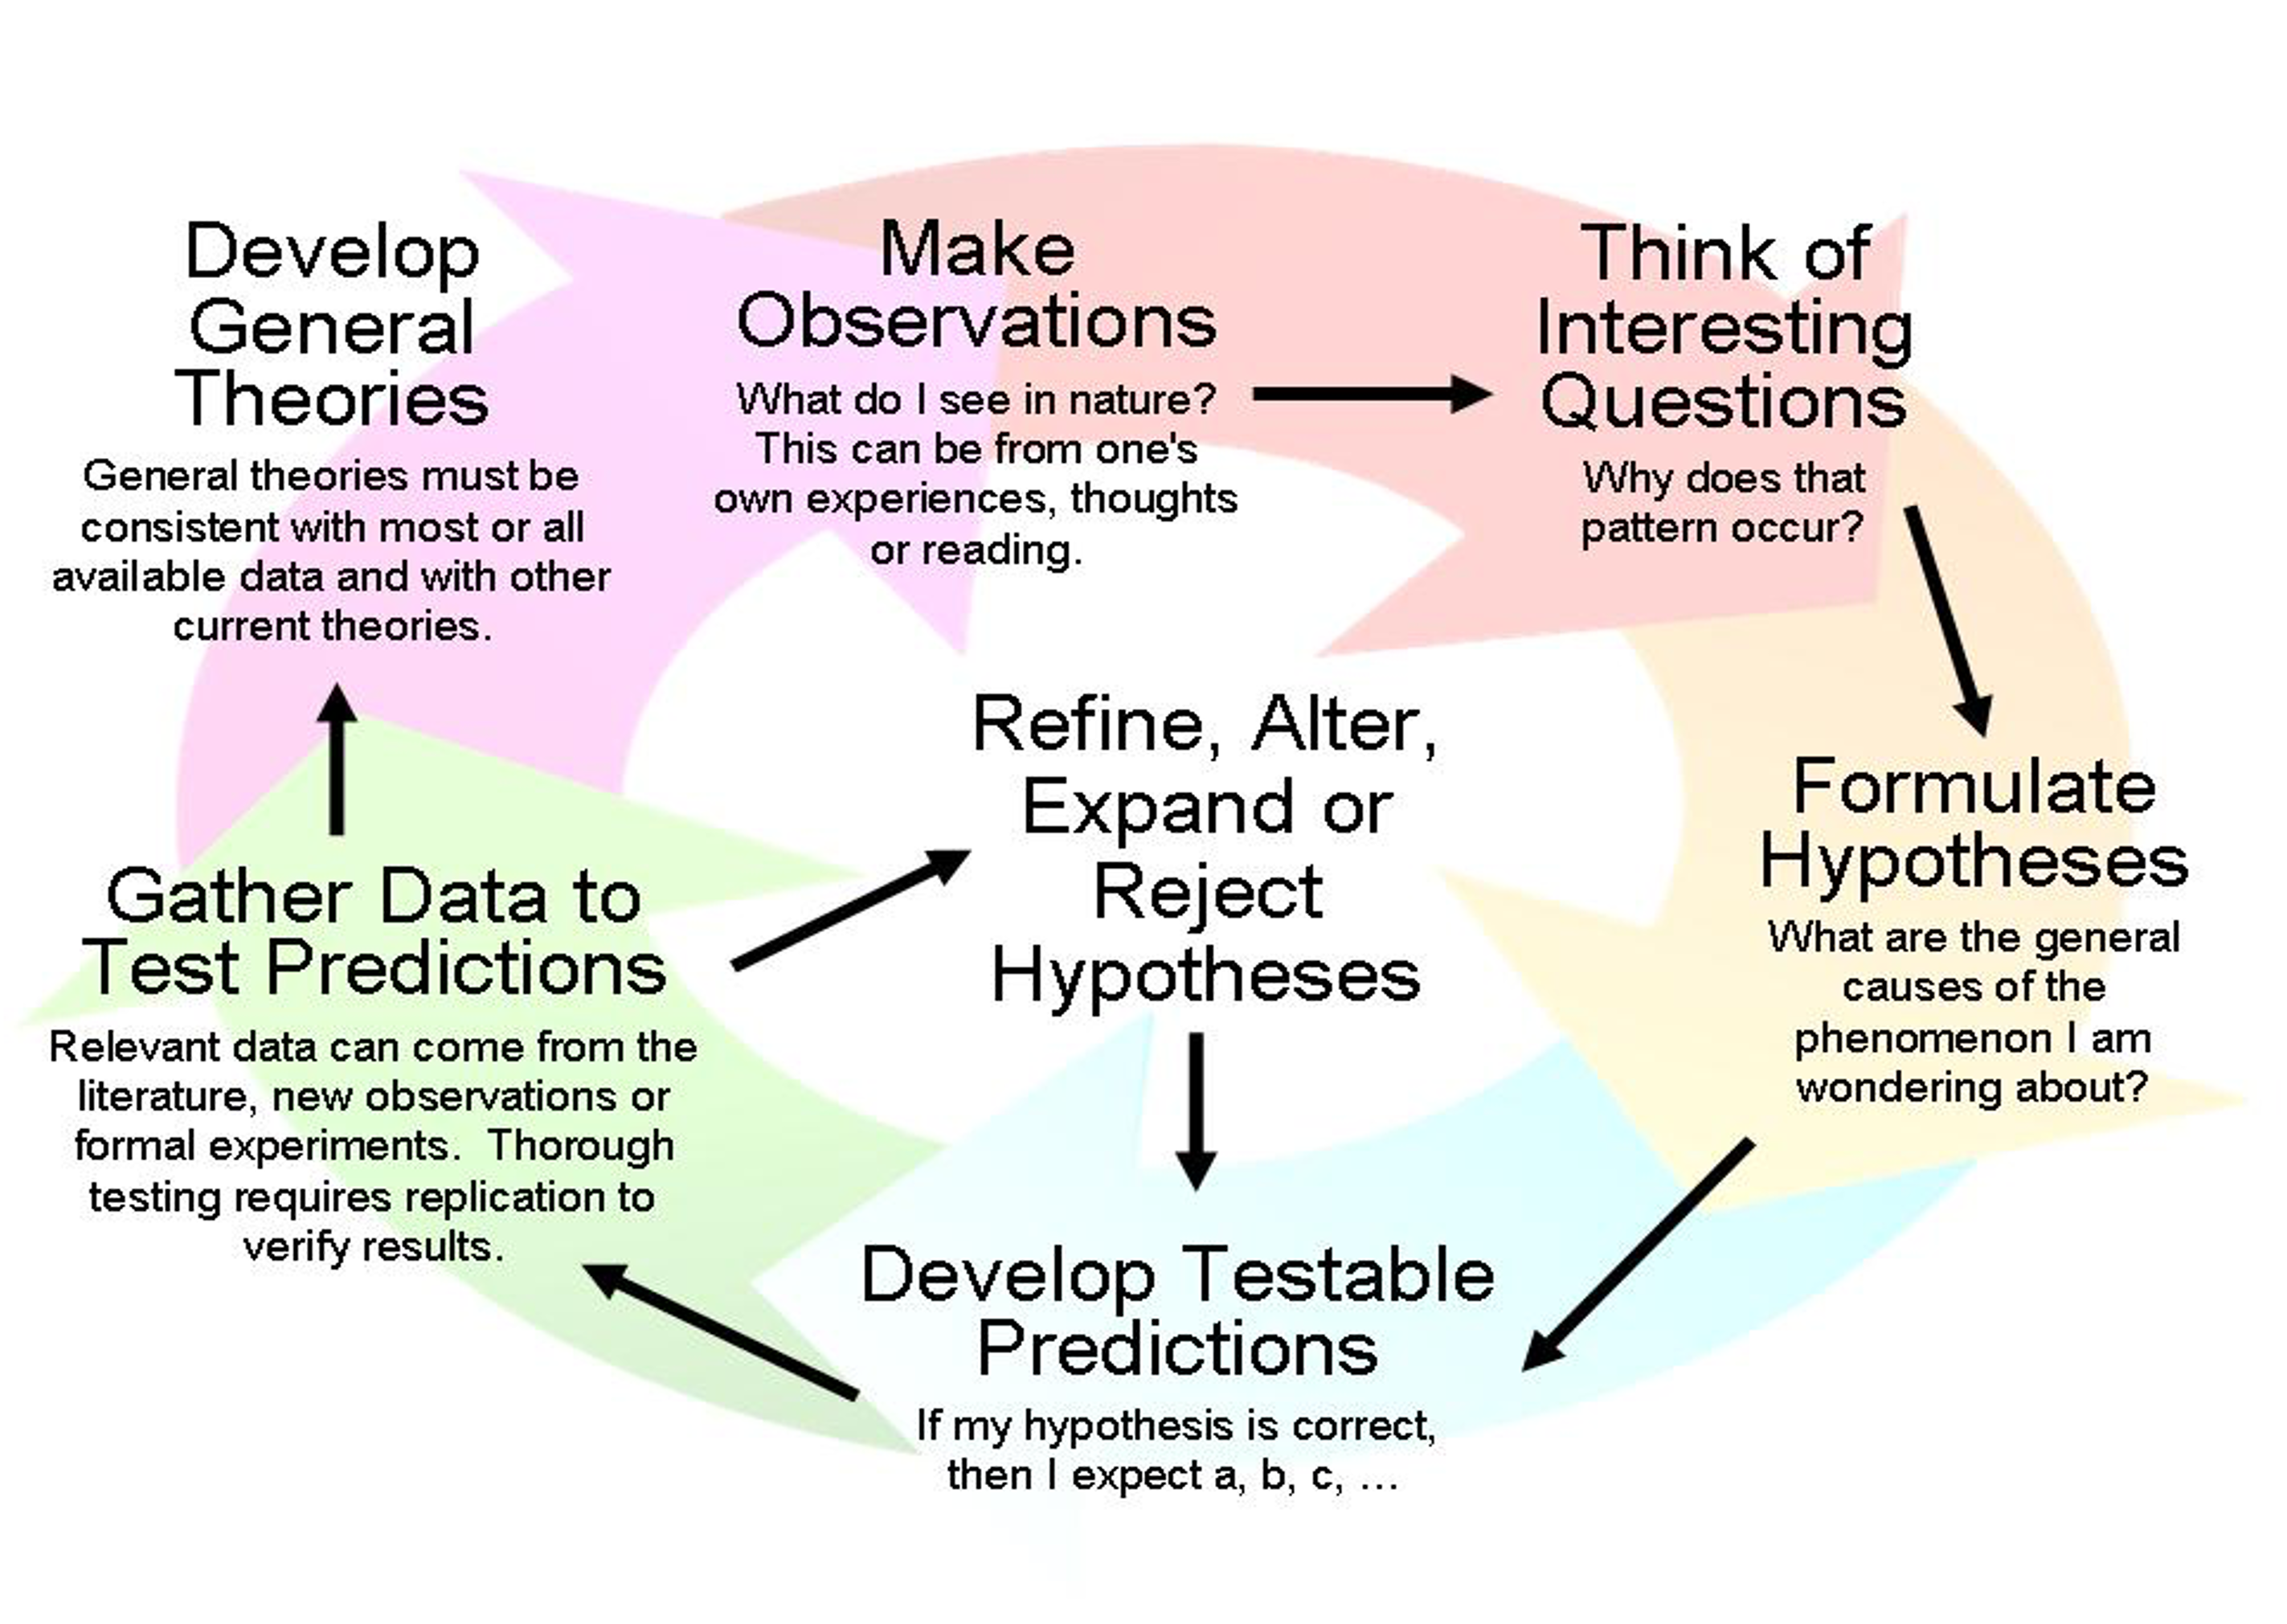
\includegraphics[width=0.75\linewidth]{/Users/craig.starbuck/Library/Mobile Documents/com~apple~CloudDocs/Documents/People Analytics Book/GitHub/peopleanalytics_lifecycle_book/graphics/scientific_method} 

}

\caption{The Scientific Method}\label{fig:sci-method}
\end{figure}

An important feature of the Scientific Method, as reflected in Figure \ref{fig:sci-method}, is that the process is akin to an infinite loop in coding; that is, it never ends. New knowledge resulting from hypothesis testing prompts a new set of questions and hypotheses, which initiates a new lifecycle of scientific inquiry.

Over the years, I have adapted the scientific method into a curtailed four-step framework to help ensure a rigorous and disciplined approach is applied to the end-to-end analytical process. The four steps are (a) Discover, (b) Design, (c) Develop, and (d) Deliver.

\begin{figure}

{\centering 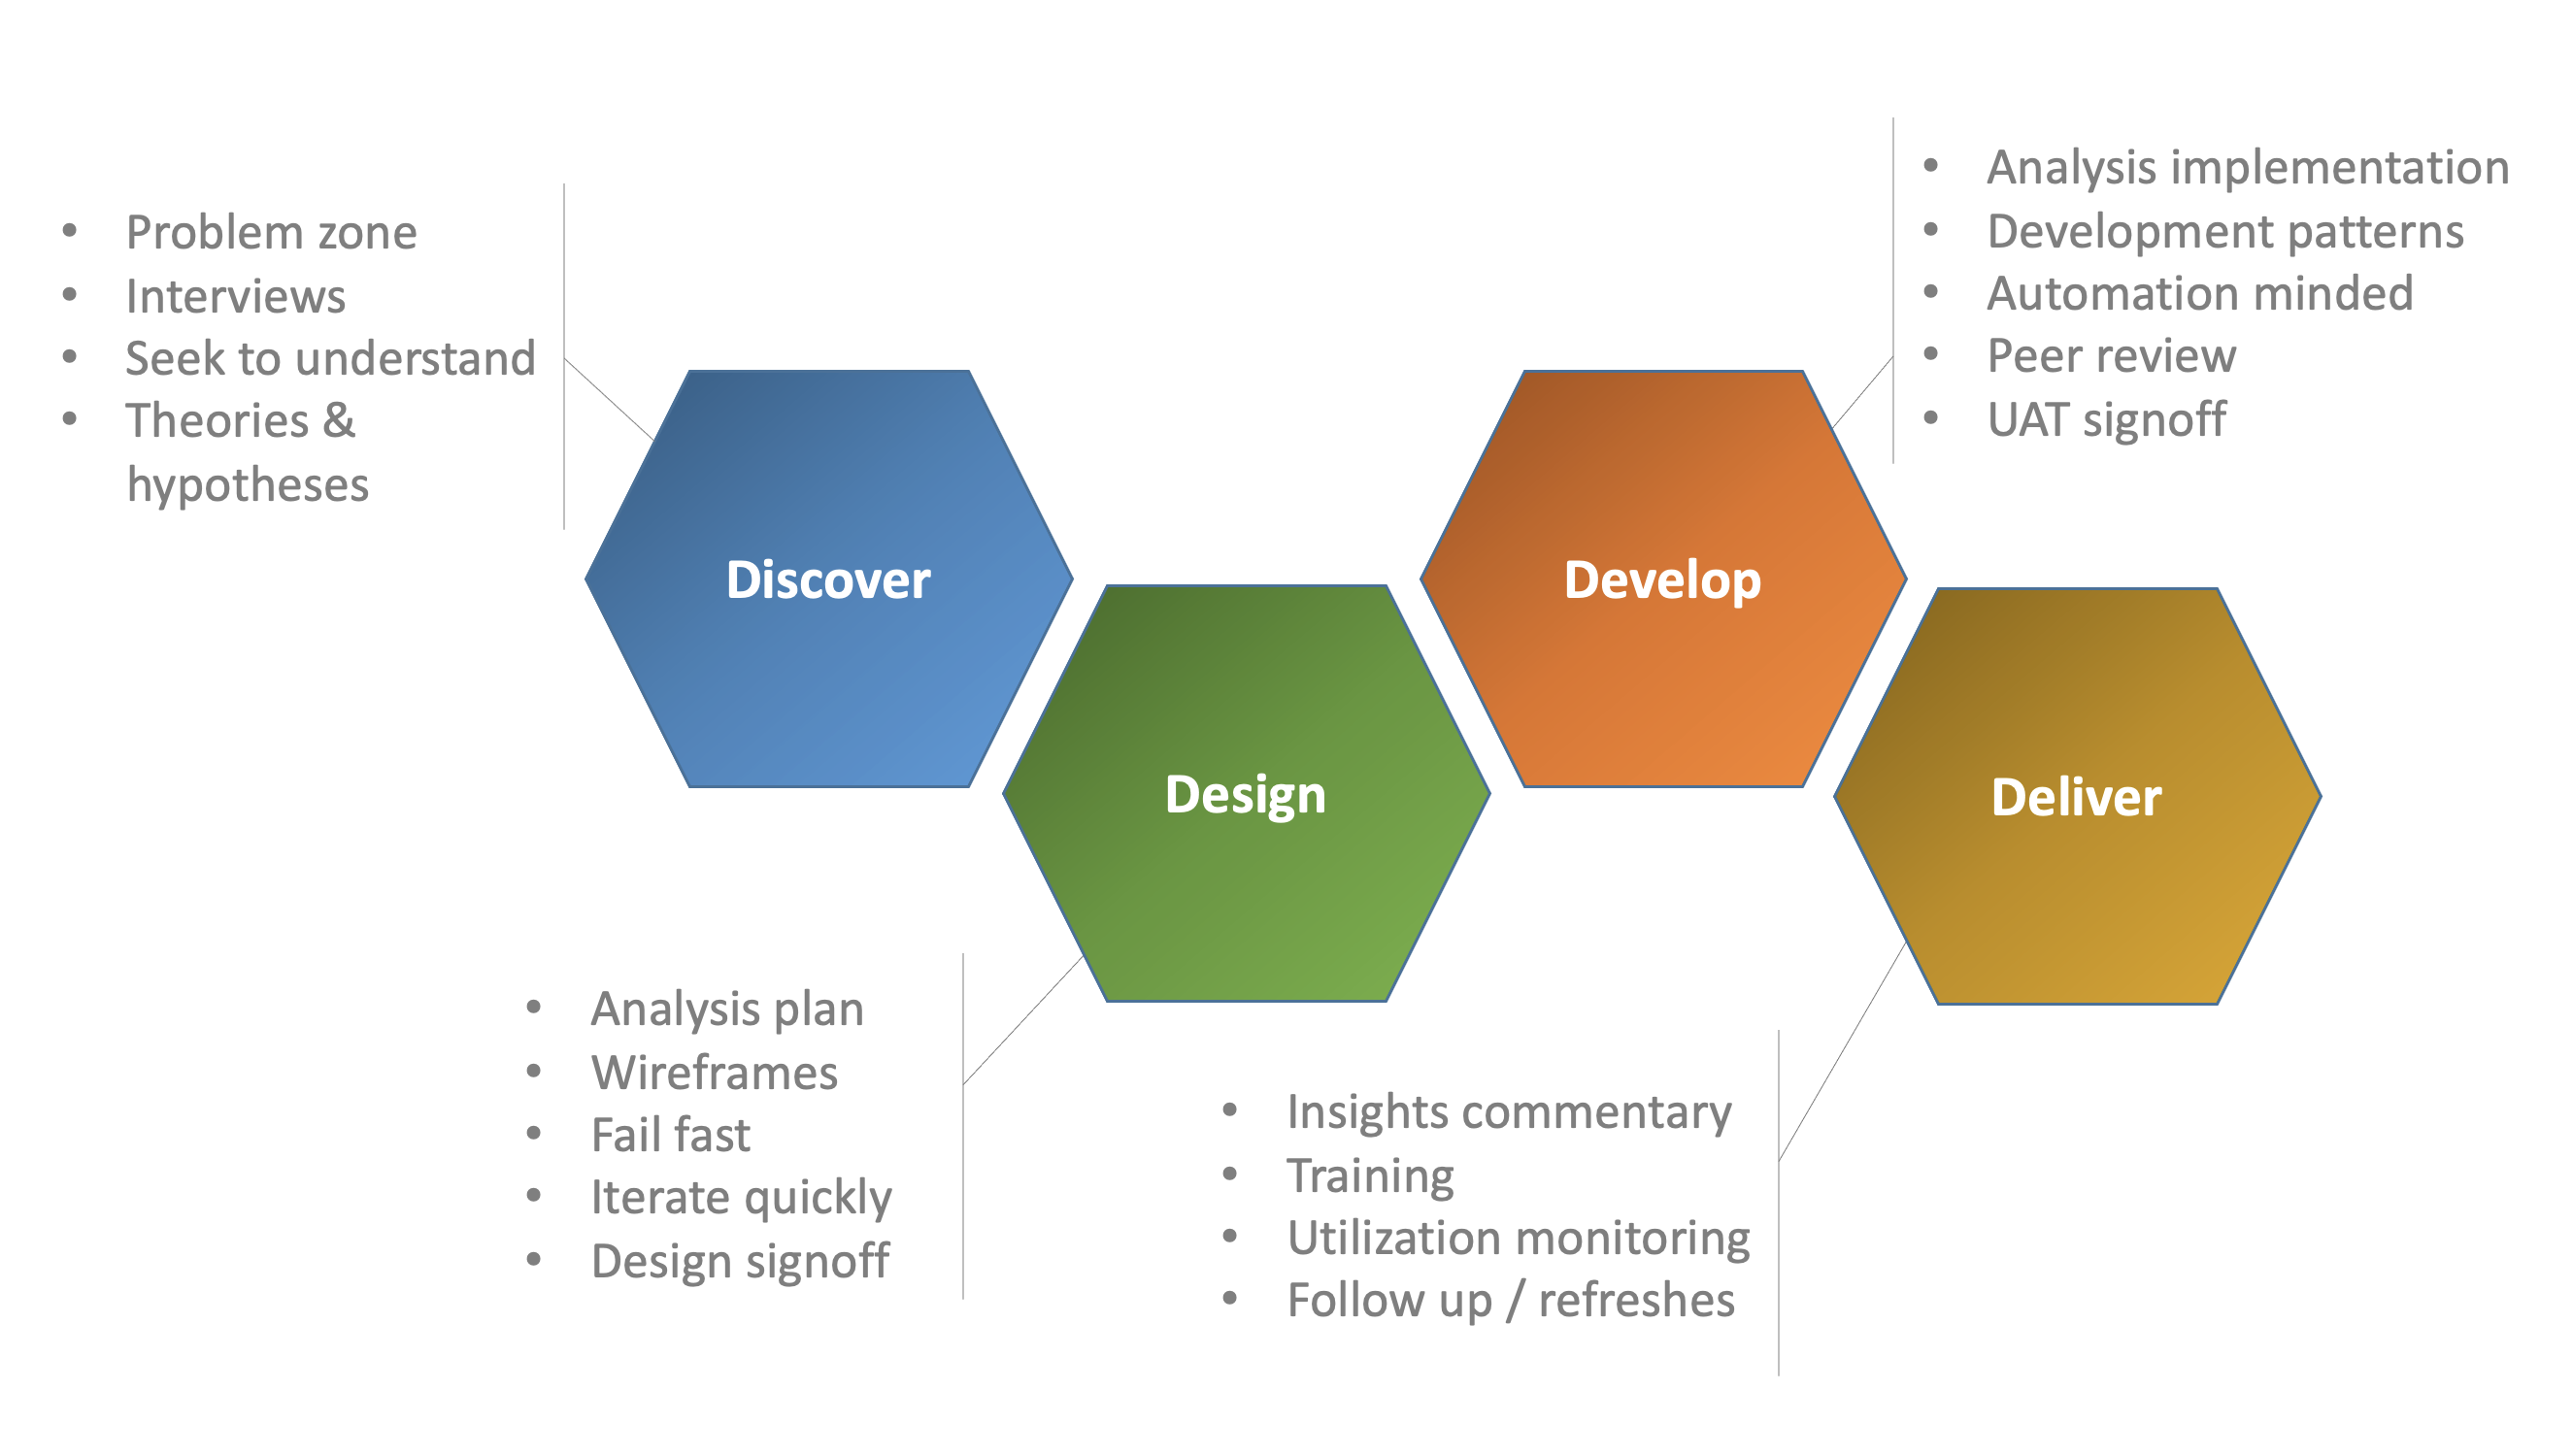
\includegraphics[width=1\linewidth]{/Users/craig.starbuck/Library/Mobile Documents/com~apple~CloudDocs/Documents/People Analytics Book/GitHub/peopleanalytics_lifecycle_book/graphics/4d_framework_overview} 

}

\caption{4D Framework}\label{fig:4d-framework}
\end{figure}

\hypertarget{discover}{%
\subsection{Discover}\label{discover}}

You are likely familiar with the following adage: ``An ounce of prevention is worth a pound of cure.'' Such is the case with respect to planning in an analytics context. During the Discover phase, it is important to remain in the problem zone; seek to understand your clients' needs through active listening and questions. This is not the time for solutioning or committing to any specific deliverables or timelines. If the client's needs are ambiguous, proceeding without clarity is unlikely to result in a favorable outcome.

It is generally helpful to think about analytics solutions -- whether a dashboard with basic metrics and trends or an advanced analysis -- like a Product Owner thinks about the initial and subsequent releases of a commercial product. A \textbf{Minimum Viable Product (MVP)} is a version of the solution with the minimum number of features to be useful to early customers who can provide feedback for future enhancements. It is important to clarify that the MVP version of solutions often has both a limited number of users and features, which protects against the tendency to boil the ocean by striving to address every question for every stakeholder. Breaking down large projects into small sets of features that are easier to communicate and adopt provides space for agility and real-time adjustments to the product roadmap per user feedback.

There are some initial questions and considerations that will help frame an analytics project and support its success.

\textbf{Client}

Who is the client? A client can be a person or organization contracting you for consulting services, or an internal stakeholder within your organization who has need. What is important to them?

\textbf{Primary Objective}

\begin{itemize}
\tightlist
\item
  What is the client ultimately hoping to accomplish?
\item
  Is the request merely to satisfy one's curiosity, or are there actions that can realistically be taken to materially influence said objective?
\end{itemize}

\textbf{Problem Statement}

\begin{itemize}
\tightlist
\item
  One of the most important early steps is clearly defining the problem statement. If your understanding of the problem -- after translating from the business terms in which it was likely initially expressed -- is misaligned with the client's needs, none of the subsequent steps matter.
\end{itemize}

\textbf{Guiding Theories}

\begin{itemize}
\tightlist
\item
  What theoretical explanations can the client offer as potential rationalizations for the phenomena of interest?
\item
  Are there existing theories in the organizational literature that should guide how the problem is tackled (e.g., findings from similar research implemented in other contexts)?
\end{itemize}

\textbf{Research Questions}

To respect the nuances of the problem statement, it is important to unpack it and frame as a set of overarching questions to guide the research.

\begin{itemize}
\tightlist
\item
  Q1: \ldots{}
\item
  Q2: \ldots{}
\item
  Q3: \ldots{}
\end{itemize}

\textbf{Research Hypotheses}

Once research questions are developed, what do you expect to find based on anecdotal stories or empirical findings? As a next step, these expectations should be expressed in the form of research hypotheses. Please note that these research hypotheses are different from statistical hypotheses (both will be covered in detail in later chapters).

\begin{itemize}
\tightlist
\item
  H1: \ldots{}
\item
  H2: \ldots{}
\item
  H3: \ldots{}
\end{itemize}

To ensure the hypotheses lend to actionable analyses, it is important to consider the following: ``What does success look like?'' In other words, once the project is complete, against which success measures will the project's success be determined? Curiosity is not a business reason and hope is not a reasonable strategy. The following questions may prove helpful in the promotion of actionable -- over merely interesting -- outcomes:

\begin{itemize}
\tightlist
\item
  What will be done if the hypotheses are empirically supported?
\item
  What will be done if the hypotheses are \emph{not} empirically supported?
\end{itemize}

\textbf{Assumptions}

At this point, it's helpful to consider what assumptions may be embedded in this discovery work. Are the questions and hypotheses rooted in what the client has theorized, or are these the product of an ambiguous understanding of the client's needs?

\textbf{Cadence}

\begin{itemize}
\tightlist
\item
  Is this analysis a one-off, or could there be a need to refresh this analysis on a regular cadence?
\item
  Are there dates associated with programs or actions this analysis is intended to support?
\end{itemize}

\textbf{Aggregation}

Is there a need for individual-level detail supporting the analysis? Aaggregate data should generally be the default unless a compelling justification exists and approval from legal and privacy partners is granted. One important role of analysts is to help keep the audience focused on the bigger picture and findings. Access to individual-level detail can not only introduce unnecessary legal and compliance risk but can also lead to questions and probing that can delay taking needed actions based on the results.

\textbf{Deliverable}

What is the preferred method of communicating the results of the analysis (e.g., interactive dashboard, static slide deck, document)? It is important to determine this early so that subsequent efforts can be structured to support the preferred deliverable. For example, if an interactive dashboard is preferred, does your Engineering department need to prioritize dependent tasks such as data pipelines, row-level security, BI development, and migrations to production servers?

\textbf{Filters \& Dimensions}

How does your client prefer to segment the workforce? Some common grouping dimensions are business unit, division, team, job family, location, tenure, and management level, but the client may have custom segmentation requirements that will be important to identify and define early in the project.

\hypertarget{design}{%
\subsection{Design}\label{design}}

Perhaps the most important initial question to answer in the design phase is: ``Does anything already exist that addresses part, or all, of the client's objectives?'' If an existing solution will suffice, or a previous analysis can be easily refreshed with recent data, it may be possible to allocate time and resources elsewhere. If related or complimentary analyses have already been performed, they may accelerate new analyses.

The end-user experience is of paramount importance during the Design phase, as solutions should have a consistent look and feel regardless of who developed them. Defining and implementing design guidelines will ensure consistency across analytics projects, as well as within large projects in which multiple analysts are collaborating on various elements of the solution.

\textbf{Data Privacy}

Are there potential concerns with the study's objective, planned actions, and/or requested data elements from an employee privacy or legal perspective? A cross-functional data governance committee can help with efficient and consistent decisioning on requests for people data and analytics.

In cases where sensitive attributes such as gender, ethnicity, age, sexual orientation, and disability status are requested, it's always best to exercise a `safety first' mentality and consult with legal and privacy partners to ensure there is comfort with the intended use of the data. The decision on whether or not to include these sensitive data elements is often less about what the audience can view (e.g., People Partners may already have access to the information at the person level in the source system) and more anchored in what they plan to do with the information.

\textbf{Data Sources \& Elements}

Is the required data already accessible in a data warehouse or other analytics environment? If not, does it need to be? What is required to achieve this?

\begin{itemize}
\tightlist
\item
  What data sources are required?
\item
  What data elements are required?
\end{itemize}

\textbf{Data Quality}

It is important to understand the data generative process and never make assumptions about how anomalies or missing data should be interpreted. After identifying what data sources will be required for a particular analysis, it is important to meet with source system owners and data stewards to deeply understand the business processes by which data are generated in the system(s). An ideal should always be \emph{unimpeachable} data quality at the analysis presentation stage, and this begins with an early understanding and investigation of data quality in the source systems. Below are some helpful questions to consider:

\begin{itemize}
\tightlist
\item
  Is there a better data source, such as data generated further upstream?
\item
  Are the data actively validated with automated data quality checks and regular exceptions reports?
\item
  What is the SLA for the data refreshes, and how often is this SLA met?
\item
  Is there a clear (and accessible) data source owner/steward?
\item
  Is there comprehensive documentation and field definitions?
\item
  Do the tables drive business critical deliverables?
\item
  Who are the other consumers of the data?
\end{itemize}

\textbf{Variables}

How will the constructs be measured (e.g., survey instrument, derived attribute, calculated field)?

\textbf{Analysis Method}

What are the appropriate analysis methods based on the research hypotheses? If modeling is required, is it more important to index on accuracy or interpretability?

\textbf{Dependencies}

Are other teams required to develop this solution? What is the nature of the work each dependent team will perform? Are there required system configuration changes? Do these teams have capacity to support?

\textbf{Change Management}

Will this solution impact current processes or solutions? If so, what is the change management plan to facilitate a seamless transition and user experience?

\textbf{Sign-Off}

Generally, it is best for the client to signoff on the problem statement, analysis approach, and wire frame for the deliverable (if applicable) before providing an ETA and proceeding to the development phase. This ensures alignment on the client's needs and the perceived utility of the solution in addressing those needs.

\hypertarget{develop}{%
\subsection{Develop}\label{develop}}

While development patterns can vary widely across analytics teams, establishing a set of standards can pay dividends in the form of greater efficiency and reliability over time. Pattern-based development ensures analysts who were not involved in a particular project can access the code and easily and quickly understand each step of the analysis: data extraction --\textgreater{} wrangling --\textgreater{} cleaning --\textgreater{} analysis --\textgreater{} visualization.

This is one of the many reasons tools like Excel will not be covered in this book. Software like R and Python allows analysts to organize and annotate steps of the analytical process in a manner that is both logical and reproducible. In case it bears repeating, learning to code is likely the best investment one can make in the pursuit of a career in analytics.

\textbf{Development Patterns}

\begin{itemize}
\tightlist
\item
  Are there development patterns that should guide the development approach to support consistency?
\item
  Are there existing calculated fields that can/should be leveraged for derived data?
\item
  Are there best practices that should be employed to optimize performance (e.g., load time for dashboards, executing complex queries during non-peak times)?
\item
  Are there standard color palettes that should be applied?
\end{itemize}

\textbf{Productionalizable Code}

\begin{itemize}
\tightlist
\item
  How do models and data science pipelines need to be developed to facilitate a seamless migration from lower to upper environments? For example, initial exploratory data analysis (EDA) may be performed using curated data in flat files for the purpose of identifying meaningful trends, relationships, and differences, but where will this data need to be sourced in production to automate the refresh of models at a regular interval? If the data were provided from multiple source systems, what joins are required to integrate the data? What transformation logic or business rules need to be applied to reproduce the curated data?
\end{itemize}

\textbf{Unit Testing}

\begin{itemize}
\tightlist
\item
  What test cases will ensure the veracity of data?
\item
  Who will perform the testing?
\end{itemize}

\textbf{UAT Testing}

\begin{itemize}
\tightlist
\item
  In the spirit of agility and constant contact with the client to prevent surprises, it is generally a good idea to have the client take the solution for a test run within the UAT environment and then provide sign-off before migrating to production. If the deliverable is a deck or doc with results from a model, UAT may surface clarifying questions that can be addressed before releasing to the broader audience.
\end{itemize}

\hypertarget{deliver}{%
\subsection{Deliver}\label{deliver}}

The Deliver phase can take many forms depending on the solution being released. If the solution is designed for a large user base, a series of recorded trainings may be in order so that there is a helpful reference for those unable to attend the live sessions or new joiners in the future. It is important to monitor success measures, which could be insights aligned to research hypotheses, dashboard utilization metrics, progress following data-informed interventions, or any number of others defined within the Discover phase.

\hypertarget{r-intro}{%
\chapter{Introduction to R}\label{r-intro}}

This chapter covers how to install R, R Studio, and required packages for replicating examples in this book. This chapter also covers R basics such as objects, data structures, and data types that are fundamental to working in R. In addition, many common functions will be covered in this chapter, and many more will be introduced throughout later chapters.

\hypertarget{getting-started-1}{%
\section{Getting Started}\label{getting-started-1}}

Run and test your code frequently. Writing a significant number of lines before testing will make debugging your code far more difficult and time-intensive than it needs to be.

\textbf{Installing R}

R can be compiled and ran on a variety of platforms including UNIX, Windows, and MacOS. R can be downloaded here: \url{https://www.r-project.org/}

When installing R, you will need to select a CRAN mirror. The \textbf{Comprehensive R Archive Network (CRAN)} is a network of servers around the world that store identical, current versions of code and documentation for R. You should select the CRAN mirror nearest you to minimize network load.

\textbf{Installing R Studio}

\textbf{R Studio} is an \textbf{Integrated Development Environment (IDE)} for R. R Studio provides a console with syntax editing that is helpful for debugging code as well as tools for plotting, history, and workspace management. Both open source and commercial editions are available, but the open-source option is sufficient for replicating everything in this book.

R Studio can be downloaded here: \url{https://www.rstudio.com/products/rstudio/download/\#download}

\textbf{Installing Packages}

Libraries from several R packages will be utilized in this book. The line of code below can be executed within R or R Studio to install all at once:

\begin{Shaded}
\begin{Highlighting}[]
\FunctionTok{install.packages}\NormalTok{(}\FunctionTok{c}\NormalTok{(}\StringTok{"tidyverse"}\NormalTok{, }\StringTok{"corrplot"}\NormalTok{, }\StringTok{"psych"}\NormalTok{, }\StringTok{"moments"}\NormalTok{, }\StringTok{"ggpubr"}\NormalTok{, }\StringTok{"GGally"}\NormalTok{, }\StringTok{"sqldf"}\NormalTok{, }\StringTok{"caret"}\NormalTok{, }\StringTok{"car"}\NormalTok{, }\StringTok{"reshape2"}\NormalTok{, }\StringTok{"flextable"}\NormalTok{, }\StringTok{"lmtest"}\NormalTok{, }\StringTok{"equatiomatic"}\NormalTok{, }\StringTok{"pwr"}\NormalTok{, }\StringTok{"nnet"}\NormalTok{, }\StringTok{"MASS"}\NormalTok{, }\StringTok{"brant"}\NormalTok{, }\StringTok{"lme4"}\NormalTok{, }\StringTok{"lmerTest"}\NormalTok{, }\StringTok{"rpart"}\NormalTok{, }\StringTok{"rpart.plot"}\NormalTok{), }\AttributeTok{dependencies =} \ConstantTok{TRUE}\NormalTok{, }\AttributeTok{repos =} \StringTok{"http://cran.us.r{-}project.org"}\NormalTok{)}
\end{Highlighting}
\end{Shaded}

\begin{verbatim}
## 
##   There are binary versions available but the source versions are later:
##            binary source needs_compilation
## texPreview    1.5  2.0.0             FALSE
## corrplot     0.89   0.92             FALSE
## psych       2.2.3  2.2.5             FALSE
## moments      0.14 0.14.1             FALSE
## caret      6.0-91 6.0-92              TRUE
## car        3.0-12  3.1-0             FALSE
## flextable   0.7.0  0.7.2             FALSE
## MASS       7.3-56 7.3-57              TRUE
## lme4       1.1-28 1.1-29              TRUE
## rpart.plot  3.1.0  3.1.1             FALSE
## 
## 
## The downloaded binary packages are in
##  /var/folders/b1/0nnhbsx55hvfb1b3n83x0qrw0000gn/T//Rtmp01G0Cg/downloaded_packages
\end{verbatim}

\textbf{Case Sensitivity}

It's important to note that everything in R is case-sensitive. When working with functions, be sure to match the case when typing the function name. For example, \texttt{Mean()} is not the same as \texttt{mean()}; since \texttt{mean()} is the correct case for the function, capitalized characters will result in an error when executing the function.

\textbf{Help}

Documentation for functions is available via the \texttt{?} command. This can be inserted prior to any function to access the function's documentation. For example, \texttt{?mean} will display the documentation, including its required and optional arguments, for the \texttt{mean()} function.

\begin{figure}

{\centering 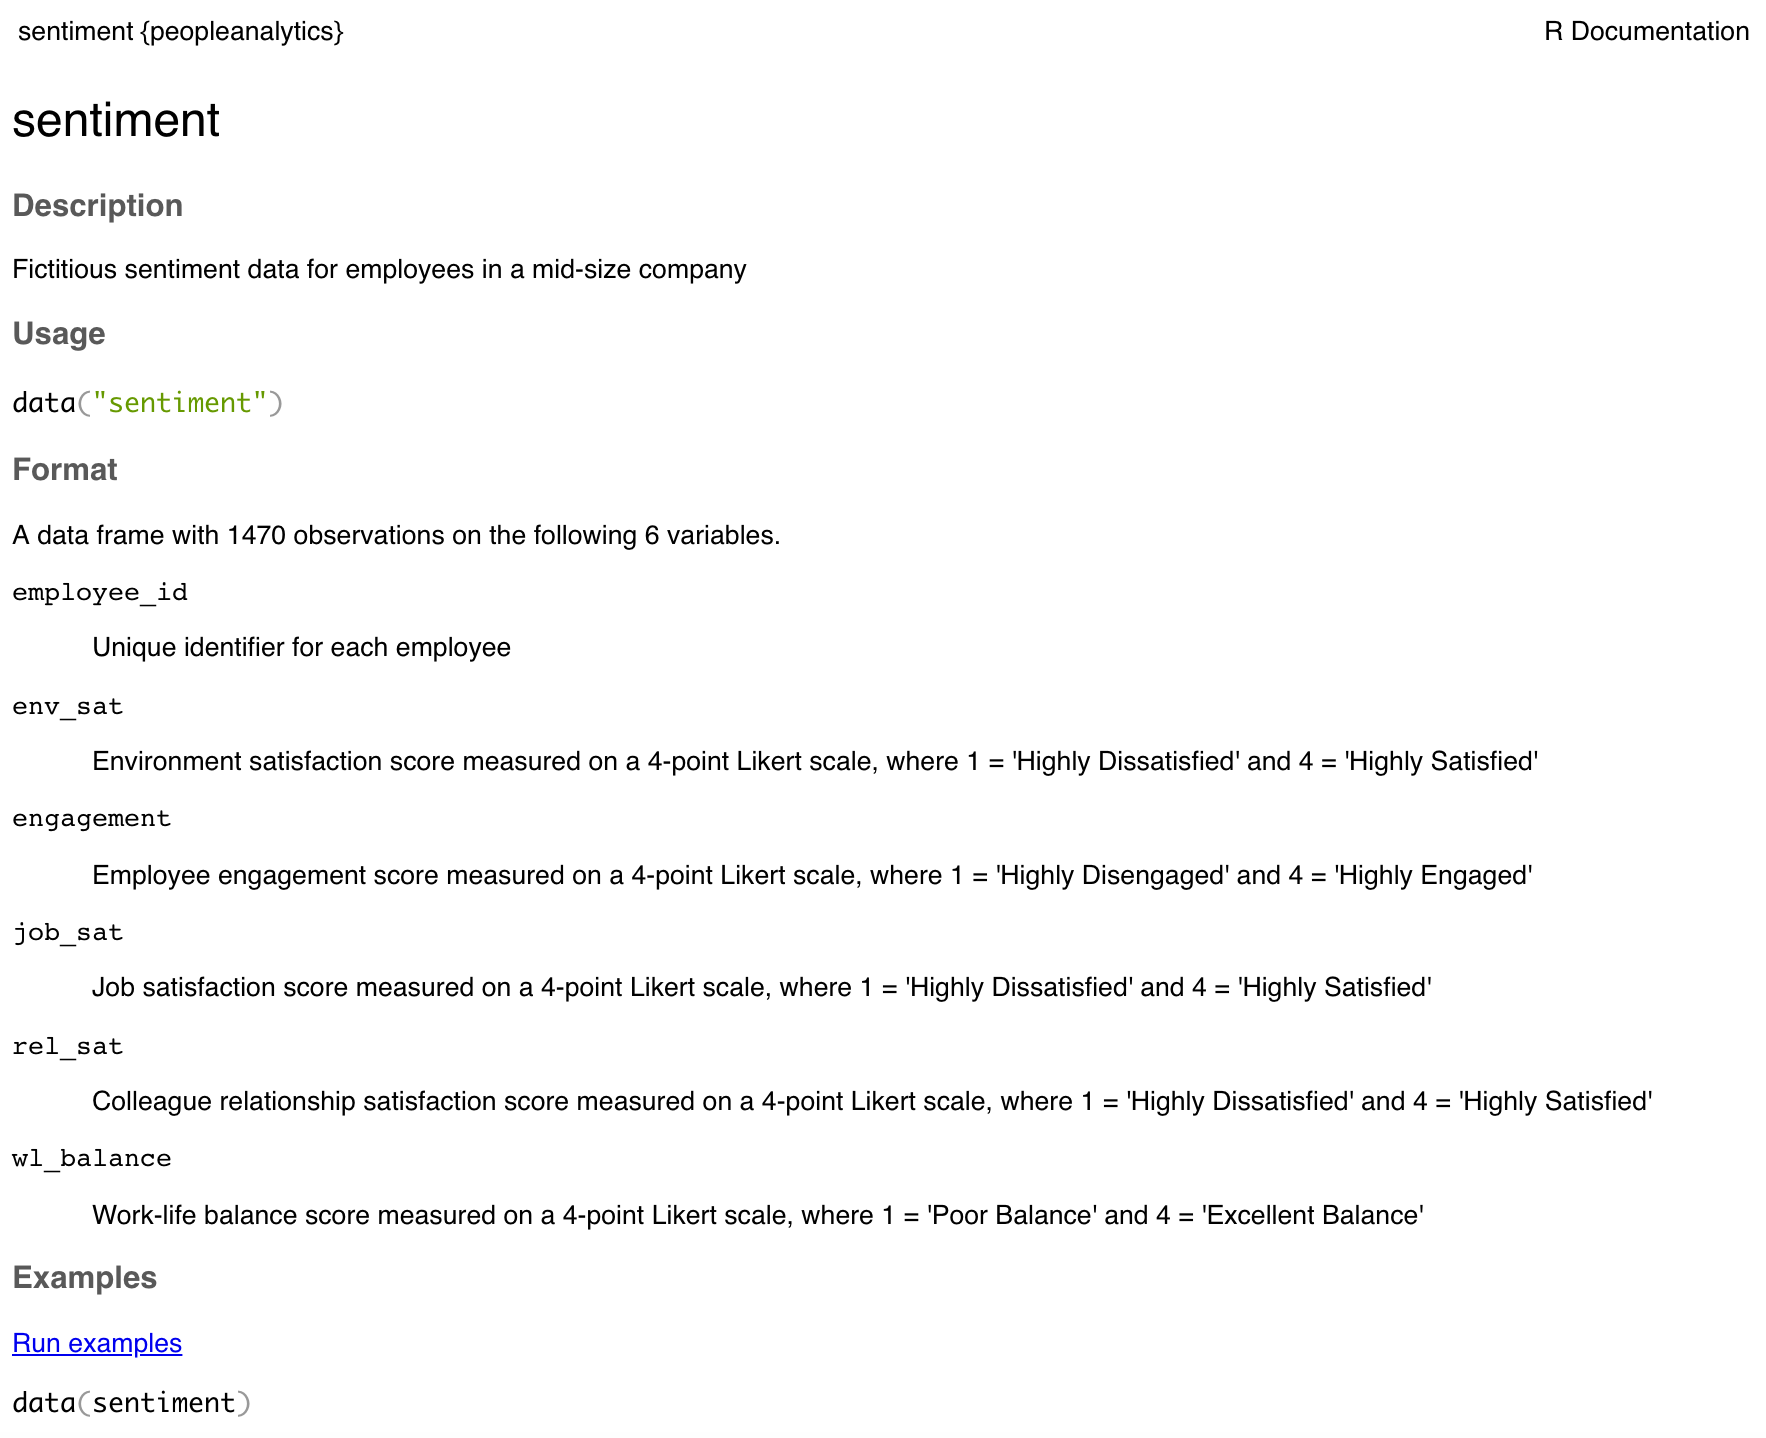
\includegraphics[width=1\linewidth]{/Users/craig.starbuck/Library/Mobile Documents/com~apple~CloudDocs/Documents/People Analytics Book/GitHub/peopleanalytics_lifecycle_book/graphics/r_help} 

}

\caption{Documentation for Arithmetic Mean Function}\label{fig:r-help}
\end{figure}

\textbf{Objects}

Objects underpin just about everything we do in R. An object is a container for various types of data. Objects can take many forms, ranging from simple objects holding a single number or character to complex structures that support advanced visualizations. The assignment character \texttt{\textless{}-} is used to assign values to an object.

Let's use the assignment operator to assign a number and character to separate objects. Note that non-numeric values must be enveloped in either single ticks \texttt{\textquotesingle{}\textquotesingle{}} or double quotes \texttt{""}:

\begin{Shaded}
\begin{Highlighting}[]
\NormalTok{obj\_1 }\OtherTok{\textless{}{-}} \DecValTok{1}
\NormalTok{obj\_1}
\end{Highlighting}
\end{Shaded}

\begin{verbatim}
## [1] 1
\end{verbatim}

\begin{Shaded}
\begin{Highlighting}[]
\NormalTok{obj\_2 }\OtherTok{\textless{}{-}} \StringTok{\textquotesingle{}a\textquotesingle{}}
\NormalTok{obj\_2}
\end{Highlighting}
\end{Shaded}

\begin{verbatim}
## [1] "a"
\end{verbatim}

Several functions are available for returning the type of data in an object:

\begin{Shaded}
\begin{Highlighting}[]
\FunctionTok{typeof}\NormalTok{(obj\_2)}
\end{Highlighting}
\end{Shaded}

\begin{verbatim}
## [1] "character"
\end{verbatim}

\begin{Shaded}
\begin{Highlighting}[]
\FunctionTok{class}\NormalTok{(obj\_2)}
\end{Highlighting}
\end{Shaded}

\begin{verbatim}
## [1] "character"
\end{verbatim}

\textbf{Comments}

The \texttt{\#} symbol is used for commenting/annotating code. This is a best practice to aid in quickly and easily deciphering the role of each line or block of code. Without comments, troubleshooting large scripts can be a more challenging task than necessary.

\begin{Shaded}
\begin{Highlighting}[]
\CommentTok{\# Assign a new number to the object named obj\_1}
\NormalTok{obj\_1 }\OtherTok{\textless{}{-}} \DecValTok{2}
\CommentTok{\# Display value in obj\_1}
\NormalTok{obj\_1}
\end{Highlighting}
\end{Shaded}

\begin{verbatim}
## [1] 2
\end{verbatim}

\begin{Shaded}
\begin{Highlighting}[]
\CommentTok{\# Assign a new character to the object named obj\_2}
\NormalTok{obj\_2 }\OtherTok{\textless{}{-}} \StringTok{\textquotesingle{}b\textquotesingle{}}
\CommentTok{\# Display value in obj\_2}
\NormalTok{obj\_2}
\end{Highlighting}
\end{Shaded}

\begin{verbatim}
## [1] "b"
\end{verbatim}

In-line code comments can also be added where needed to reduce the number of lines in a script:

\begin{Shaded}
\begin{Highlighting}[]
\CommentTok{\# Assign a new number to the object named obj\_1}
\NormalTok{obj\_1 }\OtherTok{\textless{}{-}} \DecValTok{3}
\NormalTok{obj\_1 }\CommentTok{\# Display value in obj\_1}
\end{Highlighting}
\end{Shaded}

\begin{verbatim}
## [1] 3
\end{verbatim}

\begin{Shaded}
\begin{Highlighting}[]
\CommentTok{\# Assign a new character to the object named obj\_2}
\NormalTok{obj\_2 }\OtherTok{\textless{}{-}} \StringTok{\textquotesingle{}c\textquotesingle{}} 
\NormalTok{obj\_2 }\CommentTok{\# Display value in obj\_2}
\end{Highlighting}
\end{Shaded}

\begin{verbatim}
## [1] "c"
\end{verbatim}

\hypertarget{vectors}{%
\section{Vectors}\label{vectors}}

A \textbf{vector} is the most basic data object in R. Vectors contain a collection of data elements of the same data type. For example, a vector may contain a series of numbers, set of characters, collection of dates, or logical \texttt{TRUE} or \texttt{FALSE} results.

In this example, we introduce the combine function \texttt{c()}, which allows us to fill an object with more than one value:

\begin{Shaded}
\begin{Highlighting}[]
\CommentTok{\# Create and fill a numeric vector named vect\_num}
\NormalTok{vect\_num }\OtherTok{\textless{}{-}} \FunctionTok{c}\NormalTok{(}\DecValTok{2}\NormalTok{,}\DecValTok{4}\NormalTok{,}\DecValTok{6}\NormalTok{,}\DecValTok{8}\NormalTok{,}\DecValTok{10}\NormalTok{)}
\NormalTok{vect\_num}
\end{Highlighting}
\end{Shaded}

\begin{verbatim}
## [1]  2  4  6  8 10
\end{verbatim}

\begin{Shaded}
\begin{Highlighting}[]
\CommentTok{\# Create and fill a character vector named vect\_char}
\NormalTok{vect\_char }\OtherTok{\textless{}{-}} \FunctionTok{c}\NormalTok{(}\StringTok{\textquotesingle{}a\textquotesingle{}}\NormalTok{,}\StringTok{\textquotesingle{}b\textquotesingle{}}\NormalTok{,}\StringTok{\textquotesingle{}c\textquotesingle{}}\NormalTok{)}
\NormalTok{vect\_char}
\end{Highlighting}
\end{Shaded}

\begin{verbatim}
## [1] "a" "b" "c"
\end{verbatim}

We can use the \texttt{as.Date()} function to convert character strings containing dates to an actual date data type. By default, anything within single ticks or double quotes is treated as a character, so we must make an \textbf{explicit type conversion} from characters to dates. Remember that R is case-sensitive. Therefore, \texttt{as.date()} is not a valid function; the \texttt{D} must be capitalized.

\begin{Shaded}
\begin{Highlighting}[]
\CommentTok{\# Create and fill a date vector named vect\_dt}
\NormalTok{vect\_dt }\OtherTok{\textless{}{-}} \FunctionTok{c}\NormalTok{(}\FunctionTok{as.Date}\NormalTok{(}\StringTok{"2021{-}01{-}01"}\NormalTok{), }\FunctionTok{as.Date}\NormalTok{(}\StringTok{"2022{-}01{-}01"}\NormalTok{))}
\NormalTok{vect\_dt}
\end{Highlighting}
\end{Shaded}

\begin{verbatim}
## [1] "2021-01-01" "2022-01-01"
\end{verbatim}

We can use the sequence generation function \texttt{seq()} to fill values between a start and end point using a specified interval. For example, we can fill \texttt{vect\_dt} with the first day of each month between \texttt{2021-01-01} and \texttt{2022-01-01} via the \texttt{seq()} function and its \texttt{by\ =\ "months"} argument:

\begin{Shaded}
\begin{Highlighting}[]
\CommentTok{\# Create and fill a date vector named vect\_dt}
\NormalTok{vect\_dt }\OtherTok{\textless{}{-}} \FunctionTok{seq}\NormalTok{(}\FunctionTok{as.Date}\NormalTok{(}\StringTok{"2021{-}01{-}01"}\NormalTok{), }\FunctionTok{as.Date}\NormalTok{(}\StringTok{"2022{-}01{-}01"}\NormalTok{), }\AttributeTok{by =} \StringTok{\textquotesingle{}months\textquotesingle{}}\NormalTok{)}
\NormalTok{vect\_dt}
\end{Highlighting}
\end{Shaded}

\begin{verbatim}
##  [1] "2021-01-01" "2021-02-01" "2021-03-01" "2021-04-01" "2021-05-01"
##  [6] "2021-06-01" "2021-07-01" "2021-08-01" "2021-09-01" "2021-10-01"
## [11] "2021-11-01" "2021-12-01" "2022-01-01"
\end{verbatim}

We can also use the \texttt{:} operator to fill integers between a starting and ending number:

\begin{Shaded}
\begin{Highlighting}[]
\CommentTok{\# Create and fill a numeric vector with values between 1 and 10}
\NormalTok{vect\_num }\OtherTok{\textless{}{-}} \DecValTok{1}\SpecialCharTok{:}\DecValTok{10}
\NormalTok{vect\_num}
\end{Highlighting}
\end{Shaded}

\begin{verbatim}
##  [1]  1  2  3  4  5  6  7  8  9 10
\end{verbatim}

We can access a particular element of a vector using its index. An \textbf{index} represents the position in a set of elements. In R, the first element of a vector has an index of 1, and the final element of a vector has an index equal to the vector's length. The index is specified using square brackets, such as \texttt{{[}5{]}} for the fifth element of a vector.

\begin{Shaded}
\begin{Highlighting}[]
\CommentTok{\# Return the value in position 5 of vect\_num}
\NormalTok{vect\_num[}\DecValTok{5}\NormalTok{]}
\end{Highlighting}
\end{Shaded}

\begin{verbatim}
## [1] 5
\end{verbatim}

When applied to a vector, the \texttt{length()} function returns the number of elements in the vector, and this can be used to dynamically return the last value of vectors.

\begin{Shaded}
\begin{Highlighting}[]
\CommentTok{\# Return the last element of vect\_num}
\NormalTok{vect\_num[}\FunctionTok{length}\NormalTok{(vect\_num)]}
\end{Highlighting}
\end{Shaded}

\begin{verbatim}
## [1] 10
\end{verbatim}

\textbf{Vectorized Operations}

\textbf{Vectorized operations (or vectorization)} underpin mathematical operations in R and greatly simplify computation. For example, if we need to perform a mathematical operation to each data element in a numeric vector, we do not need to specify each and every element explicitly. We can simply apply the operation at the vector level, and the operation will be applied to each of the vector's individual elements.

\begin{Shaded}
\begin{Highlighting}[]
\CommentTok{\# Create a numeric vector named x and fill with values between 1 and 10}
\NormalTok{x }\OtherTok{\textless{}{-}} \DecValTok{1}\SpecialCharTok{:}\DecValTok{10}
\end{Highlighting}
\end{Shaded}

\begin{Shaded}
\begin{Highlighting}[]
\CommentTok{\# Add 2 to each element of x}
\NormalTok{x\_plus2 }\OtherTok{\textless{}{-}}\NormalTok{ x}\SpecialCharTok{+}\DecValTok{2}
\NormalTok{x\_plus2}
\end{Highlighting}
\end{Shaded}

\begin{verbatim}
##  [1]  3  4  5  6  7  8  9 10 11 12
\end{verbatim}

\begin{Shaded}
\begin{Highlighting}[]
\CommentTok{\# Multiply each element of x by 2}
\NormalTok{x\_times2 }\OtherTok{\textless{}{-}}\NormalTok{ x}\SpecialCharTok{*}\DecValTok{2}
\NormalTok{x\_times2}
\end{Highlighting}
\end{Shaded}

\begin{verbatim}
##  [1]  2  4  6  8 10 12 14 16 18 20
\end{verbatim}

\begin{Shaded}
\begin{Highlighting}[]
\CommentTok{\# Square each element of x}
\NormalTok{x\_sq }\OtherTok{\textless{}{-}}\NormalTok{ x}\SpecialCharTok{\^{}}\DecValTok{2}
\NormalTok{x\_sq}
\end{Highlighting}
\end{Shaded}

\begin{verbatim}
##  [1]   1   4   9  16  25  36  49  64  81 100
\end{verbatim}

Many built-in arithmetic functions are available and compatible with vectors:

\begin{Shaded}
\begin{Highlighting}[]
\CommentTok{\# Aggregate sum of x elements}
\FunctionTok{sum}\NormalTok{(x)}
\end{Highlighting}
\end{Shaded}

\begin{verbatim}
## [1] 55
\end{verbatim}

\begin{Shaded}
\begin{Highlighting}[]
\CommentTok{\# Count of x elements}
\FunctionTok{length}\NormalTok{(x)}
\end{Highlighting}
\end{Shaded}

\begin{verbatim}
## [1] 10
\end{verbatim}

\begin{Shaded}
\begin{Highlighting}[]
\CommentTok{\# Square root of x elements}
\FunctionTok{sqrt}\NormalTok{(x)}
\end{Highlighting}
\end{Shaded}

\begin{verbatim}
##  [1] 1.000000 1.414214 1.732051 2.000000 2.236068 2.449490 2.645751 2.828427
##  [9] 3.000000 3.162278
\end{verbatim}

\begin{Shaded}
\begin{Highlighting}[]
\CommentTok{\# Natural logarithm of x elements}
\FunctionTok{log}\NormalTok{(x)}
\end{Highlighting}
\end{Shaded}

\begin{verbatim}
##  [1] 0.0000000 0.6931472 1.0986123 1.3862944 1.6094379 1.7917595 1.9459101
##  [8] 2.0794415 2.1972246 2.3025851
\end{verbatim}

\begin{Shaded}
\begin{Highlighting}[]
\CommentTok{\# Exponential of x elements}
\FunctionTok{exp}\NormalTok{(x)}
\end{Highlighting}
\end{Shaded}

\begin{verbatim}
##  [1]     2.718282     7.389056    20.085537    54.598150   148.413159
##  [6]   403.428793  1096.633158  2980.957987  8103.083928 22026.465795
\end{verbatim}

We can also perform various operations on multiple vectors. Vectorization will result in an implied ordering about the elements, in that the specified operation will be applied to the first elements of the vectors and then the second, then third, etc.

\begin{Shaded}
\begin{Highlighting}[]
\CommentTok{\# Create vectors x1 and x2 and fill with integers}
\NormalTok{x1 }\OtherTok{\textless{}{-}} \DecValTok{1}\SpecialCharTok{:}\DecValTok{10}
\NormalTok{x2 }\OtherTok{\textless{}{-}} \DecValTok{11}\SpecialCharTok{:}\DecValTok{20}

\CommentTok{\# Store sum of vectors to new x3 vector}
\NormalTok{x3 }\OtherTok{\textless{}{-}}\NormalTok{ x1 }\SpecialCharTok{+}\NormalTok{ x2}
\NormalTok{x3}
\end{Highlighting}
\end{Shaded}

\begin{verbatim}
##  [1] 12 14 16 18 20 22 24 26 28 30
\end{verbatim}

Using vectorization, we can also evaluate whether a specified condition is true or false for each element in a vector:

\begin{Shaded}
\begin{Highlighting}[]
\CommentTok{\# Evaluate whether each element of x is less than 6, and store results to a logical vector}
\NormalTok{logical\_rslts }\OtherTok{\textless{}{-}}\NormalTok{ x}\SpecialCharTok{\textless{}}\DecValTok{6}
\NormalTok{logical\_rslts}
\end{Highlighting}
\end{Shaded}

\begin{verbatim}
##  [1]  TRUE  TRUE  TRUE  TRUE  TRUE FALSE FALSE FALSE FALSE FALSE
\end{verbatim}

\hypertarget{matrices}{%
\section{Matrices}\label{matrices}}

A \textbf{matrix} is like a vector in that it represents a collection of data elements of the same data type; however, the elements of a matrix are \emph{arranged into a fixed number of rows and columns}.

We can create a matrix using the \texttt{matrix()} function. Per \texttt{?matrix}, the \texttt{nrow} and \texttt{ncol} arguments can be used to organize like data elements into a specified number of rows and columns.

\begin{Shaded}
\begin{Highlighting}[]
\CommentTok{\# Create and fill matrix with numbers}
\NormalTok{mtrx\_num }\OtherTok{\textless{}{-}} \FunctionTok{matrix}\NormalTok{(}\AttributeTok{data =} \DecValTok{1}\SpecialCharTok{:}\DecValTok{10}\NormalTok{, }\AttributeTok{nrow =} \DecValTok{5}\NormalTok{, }\AttributeTok{ncol =} \DecValTok{2}\NormalTok{)}
\NormalTok{mtrx\_num}
\end{Highlighting}
\end{Shaded}

\begin{verbatim}
##      [,1] [,2]
## [1,]    1    6
## [2,]    2    7
## [3,]    3    8
## [4,]    4    9
## [5,]    5   10
\end{verbatim}

We can leverage shorthand for function calls. As long as the argument values are in the correct order by the documentation, the argument names are not required. Per \texttt{?matrix}, the first argument is \texttt{data}, followed by \texttt{nrow} and then \texttt{ncol}. Therefore, we can achieve the same result using the following:

\begin{Shaded}
\begin{Highlighting}[]
\CommentTok{\# Create and fill matrix with numbers}
\NormalTok{mtrx\_num }\OtherTok{\textless{}{-}} \FunctionTok{matrix}\NormalTok{(}\DecValTok{1}\SpecialCharTok{:}\DecValTok{10}\NormalTok{, }\DecValTok{5}\NormalTok{, }\DecValTok{2}\NormalTok{)}
\NormalTok{mtrx\_num}
\end{Highlighting}
\end{Shaded}

\begin{verbatim}
##      [,1] [,2]
## [1,]    1    6
## [2,]    2    7
## [3,]    3    8
## [4,]    4    9
## [5,]    5   10
\end{verbatim}

Several functions are available to quickly retrieve the number of rows and columns in a rectangular object like a matrix:

\begin{Shaded}
\begin{Highlighting}[]
\CommentTok{\# Return the number of rows in mtrx\_num}
\FunctionTok{nrow}\NormalTok{(mtrx\_num)}
\end{Highlighting}
\end{Shaded}

\begin{verbatim}
## [1] 5
\end{verbatim}

\begin{Shaded}
\begin{Highlighting}[]
\CommentTok{\# Return the number of columns in mtrx\_num}
\FunctionTok{ncol}\NormalTok{(mtrx\_num)}
\end{Highlighting}
\end{Shaded}

\begin{verbatim}
## [1] 2
\end{verbatim}

\begin{Shaded}
\begin{Highlighting}[]
\CommentTok{\# Return the number of columns and rows in mtrx\_num}
\FunctionTok{dim}\NormalTok{(mtrx\_num)}
\end{Highlighting}
\end{Shaded}

\begin{verbatim}
## [1] 5 2
\end{verbatim}

The \texttt{head()} and \texttt{tail()} functions return the first and last pieces of data, respectively. For large matrices (or other types of objects), this can be helpful for previewing the data:

\begin{Shaded}
\begin{Highlighting}[]
\CommentTok{\# Return the first five rows of the matrix}
\FunctionTok{head}\NormalTok{(}\FunctionTok{matrix}\NormalTok{(}\DecValTok{1}\SpecialCharTok{:}\DecValTok{10000}\NormalTok{, }\DecValTok{1000}\NormalTok{, }\DecValTok{10}\NormalTok{), }\DecValTok{5}\NormalTok{)}
\end{Highlighting}
\end{Shaded}

\begin{verbatim}
##      [,1] [,2] [,3] [,4] [,5] [,6] [,7] [,8] [,9] [,10]
## [1,]    1 1001 2001 3001 4001 5001 6001 7001 8001  9001
## [2,]    2 1002 2002 3002 4002 5002 6002 7002 8002  9002
## [3,]    3 1003 2003 3003 4003 5003 6003 7003 8003  9003
## [4,]    4 1004 2004 3004 4004 5004 6004 7004 8004  9004
## [5,]    5 1005 2005 3005 4005 5005 6005 7005 8005  9005
\end{verbatim}

\begin{Shaded}
\begin{Highlighting}[]
\CommentTok{\# Return the last five rows of the matrix}
\FunctionTok{tail}\NormalTok{(}\FunctionTok{matrix}\NormalTok{(}\DecValTok{1}\SpecialCharTok{:}\DecValTok{10000}\NormalTok{, }\DecValTok{1000}\NormalTok{, }\DecValTok{10}\NormalTok{), }\DecValTok{5}\NormalTok{)}
\end{Highlighting}
\end{Shaded}

\begin{verbatim}
##         [,1] [,2] [,3] [,4] [,5] [,6] [,7] [,8] [,9] [,10]
##  [996,]  996 1996 2996 3996 4996 5996 6996 7996 8996  9996
##  [997,]  997 1997 2997 3997 4997 5997 6997 7997 8997  9997
##  [998,]  998 1998 2998 3998 4998 5998 6998 7998 8998  9998
##  [999,]  999 1999 2999 3999 4999 5999 6999 7999 8999  9999
## [1000,] 1000 2000 3000 4000 5000 6000 7000 8000 9000 10000
\end{verbatim}

Using vectorization, we can easily perform matrix multiplication.

\begin{Shaded}
\begin{Highlighting}[]
\CommentTok{\# Create 3x3 matrix}
\FunctionTok{matrix}\NormalTok{(}\DecValTok{1}\SpecialCharTok{:}\DecValTok{9}\NormalTok{, }\DecValTok{3}\NormalTok{, }\DecValTok{3}\NormalTok{)}
\end{Highlighting}
\end{Shaded}

\begin{verbatim}
##      [,1] [,2] [,3]
## [1,]    1    4    7
## [2,]    2    5    8
## [3,]    3    6    9
\end{verbatim}

\begin{Shaded}
\begin{Highlighting}[]
\CommentTok{\# Multiply each matrix value by 2}
\FunctionTok{matrix}\NormalTok{(}\DecValTok{1}\SpecialCharTok{:}\DecValTok{9}\NormalTok{, }\DecValTok{3}\NormalTok{, }\DecValTok{3}\NormalTok{) }\SpecialCharTok{*} \DecValTok{2}
\end{Highlighting}
\end{Shaded}

\begin{verbatim}
##      [,1] [,2] [,3]
## [1,]    2    8   14
## [2,]    4   10   16
## [3,]    6   12   18
\end{verbatim}

\hypertarget{factors}{%
\section{Factors}\label{factors}}

A \textbf{factor} is a data structure containing a finite number of categorical values. Each categorical value of a factor is known as a \textbf{level}, and the levels can be either ordered or unordered. This data structure is a requirement for several statistical models we will cover in later chapters.

We can create a factor using the \texttt{factor()} function:

\begin{Shaded}
\begin{Highlighting}[]
\CommentTok{\# Create and fill factor with unordered categories}
\NormalTok{education }\OtherTok{\textless{}{-}} \FunctionTok{factor}\NormalTok{(}\FunctionTok{c}\NormalTok{(}\StringTok{"undergraduate"}\NormalTok{, }\StringTok{"post{-}graduate"}\NormalTok{, }\StringTok{"graduate"}\NormalTok{))}
\NormalTok{education}
\end{Highlighting}
\end{Shaded}

\begin{verbatim}
## [1] undergraduate post-graduate graduate     
## Levels: graduate post-graduate undergraduate
\end{verbatim}

Since education has an inherent ordering, we can use the \texttt{ordered} and \texttt{levels} arguments of the \texttt{factor()} function to order the categories:

\begin{Shaded}
\begin{Highlighting}[]
\CommentTok{\# Create and fill factor with unordered categories}
\NormalTok{education }\OtherTok{\textless{}{-}} \FunctionTok{factor}\NormalTok{(education, }\AttributeTok{ordered =} \ConstantTok{TRUE}\NormalTok{, }\AttributeTok{levels =} \FunctionTok{c}\NormalTok{(}\StringTok{"undergraduate"}\NormalTok{, }\StringTok{"graduate"}\NormalTok{, }\StringTok{"post{-}graduate"}\NormalTok{))}
\NormalTok{education}
\end{Highlighting}
\end{Shaded}

\begin{verbatim}
## [1] undergraduate post-graduate graduate     
## Levels: undergraduate < graduate < post-graduate
\end{verbatim}

The ordering of factors is critical to a correct interpretation of statistical model output as we will cover later.

\hypertarget{data-frames}{%
\section{Data Frames}\label{data-frames}}

A \emph{data frame} is like a matrix in that it organizes elements within rows and columns but unlike matrices, data frames can store multiple types of data. Data frames are often the most appropriate data structures for the data required in people analytics.

A data frame can be created using the \texttt{data.frame()} function:

\begin{Shaded}
\begin{Highlighting}[]
\CommentTok{\# Create three vectors containing integers (x), characters (y), and dates (z)}
\NormalTok{x }\OtherTok{\textless{}{-}} \DecValTok{1}\SpecialCharTok{:}\DecValTok{10}
\NormalTok{y }\OtherTok{\textless{}{-}} \FunctionTok{c}\NormalTok{(}\StringTok{\textquotesingle{}a\textquotesingle{}}\NormalTok{,}\StringTok{\textquotesingle{}b\textquotesingle{}}\NormalTok{,}\StringTok{\textquotesingle{}c\textquotesingle{}}\NormalTok{,}\StringTok{\textquotesingle{}d\textquotesingle{}}\NormalTok{,}\StringTok{\textquotesingle{}e\textquotesingle{}}\NormalTok{,}\StringTok{\textquotesingle{}f\textquotesingle{}}\NormalTok{,}\StringTok{\textquotesingle{}g\textquotesingle{}}\NormalTok{,}\StringTok{\textquotesingle{}h\textquotesingle{}}\NormalTok{,}\StringTok{\textquotesingle{}i\textquotesingle{}}\NormalTok{,}\StringTok{\textquotesingle{}j\textquotesingle{}}\NormalTok{)}
\NormalTok{z }\OtherTok{\textless{}{-}} \FunctionTok{seq}\NormalTok{(}\FunctionTok{as.Date}\NormalTok{(}\StringTok{"2021{-}01{-}01"}\NormalTok{), }\FunctionTok{as.Date}\NormalTok{(}\StringTok{"2021{-}10{-}01"}\NormalTok{), }\AttributeTok{by =} \StringTok{\textquotesingle{}months\textquotesingle{}}\NormalTok{)}

\CommentTok{\# Create a data frame with 3 columns (vectors x, y, and z) and 10 rows}
\NormalTok{df }\OtherTok{\textless{}{-}} \FunctionTok{data.frame}\NormalTok{(x, y, z)}
\NormalTok{df}
\end{Highlighting}
\end{Shaded}

\begin{verbatim}
##     x y          z
## 1   1 a 2021-01-01
## 2   2 b 2021-02-01
## 3   3 c 2021-03-01
## 4   4 d 2021-04-01
## 5   5 e 2021-05-01
## 6   6 f 2021-06-01
## 7   7 g 2021-07-01
## 8   8 h 2021-08-01
## 9   9 i 2021-09-01
## 10 10 j 2021-10-01
\end{verbatim}

The structure of an object can be viewed using the \texttt{str()} function:

\begin{Shaded}
\begin{Highlighting}[]
\CommentTok{\# Describe the structure of df}
\FunctionTok{str}\NormalTok{(df)}
\end{Highlighting}
\end{Shaded}

\begin{verbatim}
## 'data.frame':    10 obs. of  3 variables:
##  $ x: int  1 2 3 4 5 6 7 8 9 10
##  $ y: chr  "a" "b" "c" "d" ...
##  $ z: Date, format: "2021-01-01" "2021-02-01" ...
\end{verbatim}

Specific columns in the data frame can be referenced using the \texttt{\$} symbol between the data frame and column names:

\begin{Shaded}
\begin{Highlighting}[]
\CommentTok{\# Return data in column x in df}
\NormalTok{df}\SpecialCharTok{$}\NormalTok{x}
\end{Highlighting}
\end{Shaded}

\begin{verbatim}
##  [1]  1  2  3  4  5  6  7  8  9 10
\end{verbatim}

Another method that allows for efficient subsetting of rows and/or columns is the \texttt{subset()} function. The example below illustrates how to subset \texttt{df} using conditions on \texttt{x} and \texttt{y} while only displaying \texttt{z} in the output:

\begin{Shaded}
\begin{Highlighting}[]
\CommentTok{\# Return z values for rows where x is at least 7 OR y is a, b, or c.}
\FunctionTok{subset}\NormalTok{(df, x }\SpecialCharTok{\textgreater{}=} \DecValTok{7} \SpecialCharTok{|}\NormalTok{ y }\SpecialCharTok{==} \FunctionTok{c}\NormalTok{(}\StringTok{\textquotesingle{}a\textquotesingle{}}\NormalTok{,}\StringTok{\textquotesingle{}b\textquotesingle{}}\NormalTok{,}\StringTok{\textquotesingle{}c\textquotesingle{}}\NormalTok{), }\AttributeTok{select =}\NormalTok{ z)}
\end{Highlighting}
\end{Shaded}

\begin{verbatim}
##             z
## 1  2021-01-01
## 2  2021-02-01
## 3  2021-03-01
## 7  2021-07-01
## 8  2021-08-01
## 9  2021-09-01
## 10 2021-10-01
\end{verbatim}

\hypertarget{lists}{%
\section{Lists}\label{lists}}

\textbf{Lists} are versatile objects that can contain elements with different types and lengths. The elements of a list can be vectors, matrices, data frames, functions, or even other lists.

A list can be created using the \texttt{list()} function:

\begin{Shaded}
\begin{Highlighting}[]
\CommentTok{\# Store vectors x, y, and z as well as df to a list}
\NormalTok{lst }\OtherTok{\textless{}{-}} \FunctionTok{list}\NormalTok{(x, y, z, df)}
\FunctionTok{str}\NormalTok{(lst)}
\end{Highlighting}
\end{Shaded}

\begin{verbatim}
## List of 4
##  $ : int [1:10] 1 2 3 4 5 6 7 8 9 10
##  $ : chr [1:10] "a" "b" "c" "d" ...
##  $ : Date[1:10], format: "2021-01-01" "2021-02-01" ...
##  $ :'data.frame':    10 obs. of  3 variables:
##   ..$ x: int [1:10] 1 2 3 4 5 6 7 8 9 10
##   ..$ y: chr [1:10] "a" "b" "c" "d" ...
##   ..$ z: Date[1:10], format: "2021-01-01" "2021-02-01" ...
\end{verbatim}

Unlike vectors, accessing elements of a list requires double brackets, such as \texttt{{[}{[}3{]}{]}} for the third element.

\begin{Shaded}
\begin{Highlighting}[]
\CommentTok{\# Return data from the third element of lst}
\NormalTok{lst[[}\DecValTok{3}\NormalTok{]]}
\end{Highlighting}
\end{Shaded}

\begin{verbatim}
##  [1] "2021-01-01" "2021-02-01" "2021-03-01" "2021-04-01" "2021-05-01"
##  [6] "2021-06-01" "2021-07-01" "2021-08-01" "2021-09-01" "2021-10-01"
\end{verbatim}

\hypertarget{loops}{%
\section{Loops}\label{loops}}

In many cases, the need arises to perform an operation a variable number of times. Loops are available to avoid the cumbersome task of writing the same statement many times. The two most common types of loops are \texttt{while} and \texttt{for} loops.

Let's use a \texttt{while} loop to square integers between 1 and 5:

\begin{Shaded}
\begin{Highlighting}[]
\CommentTok{\# Initialize variable}
\NormalTok{i }\OtherTok{\textless{}{-}} \DecValTok{1}

\CommentTok{\# Using a \textquotesingle{}while\textquotesingle{} loop, square the values 1 through 5 and print results to the screen}
\CommentTok{\# \textquotesingle{}i\textquotesingle{} is a variable that takes on a value between 1 and 5 for the respective loop}
\ControlFlowTok{while}\NormalTok{ (i }\SpecialCharTok{\textless{}} \DecValTok{6}\NormalTok{) \{}
  
  \FunctionTok{print}\NormalTok{(i}\SpecialCharTok{\^{}}\DecValTok{2}\NormalTok{) }
\NormalTok{  i }\OtherTok{\textless{}{-}}\NormalTok{ i }\SpecialCharTok{+} \DecValTok{1} \CommentTok{\# increment i by 1}
  
\NormalTok{\}}
\end{Highlighting}
\end{Shaded}

\begin{verbatim}
## [1] 1
## [1] 4
## [1] 9
## [1] 16
## [1] 25
\end{verbatim}

With a \texttt{while} loop, we needed to initialize the variable \texttt{i} as well as increment it by \texttt{1} within the loop. With a \texttt{for} loop, we can accomplish the same goal with less code:

\begin{Shaded}
\begin{Highlighting}[]
\CommentTok{\# Using a \textquotesingle{}for\textquotesingle{} loop, square the values 1 through 5 and print results to the screen}
\ControlFlowTok{for}\NormalTok{ (i }\ControlFlowTok{in} \DecValTok{1}\SpecialCharTok{:}\DecValTok{5}\NormalTok{) \{ }
  
  \FunctionTok{print}\NormalTok{(i}\SpecialCharTok{\^{}}\DecValTok{2}\NormalTok{)}
  
\NormalTok{\}}
\end{Highlighting}
\end{Shaded}

\begin{verbatim}
## [1] 1
## [1] 4
## [1] 9
## [1] 16
## [1] 25
\end{verbatim}

\hypertarget{user-defined-functions-udfs}{%
\section{User-Defined Functions (UDFs)}\label{user-defined-functions-udfs}}

Though many built-in functions are available, R provides the flexibility to create our own. In fact, many functions used in this book are actually functions of functions.

Functions can be an effective alternative to loops. For example, here is a basic function that achieves the same goal as our \texttt{while} and \texttt{for} loop examples (i.e., squaring integers 1 through 5):

\begin{Shaded}
\begin{Highlighting}[]
\CommentTok{\# Create a function named square.val() with one argument (x) that squares given x values}
\NormalTok{square.val }\OtherTok{\textless{}{-}} \ControlFlowTok{function}\NormalTok{(x) \{}
  
\NormalTok{  x}\SpecialCharTok{\^{}}\DecValTok{2}
\NormalTok{\}}

\CommentTok{\# Pass integers 1 through 5 into the new square.val() function and display results}
\FunctionTok{square.val}\NormalTok{(}\DecValTok{1}\SpecialCharTok{:}\DecValTok{5}\NormalTok{)}
\end{Highlighting}
\end{Shaded}

\begin{verbatim}
## [1]  1  4  9 16 25
\end{verbatim}

While many projects warrant UDFs and/or loops, we do not actually need either to square a set of integers. As you gain experience writing R code, you will naturally discover ways to write more performant and terse code:

\begin{Shaded}
\begin{Highlighting}[]
\CommentTok{\# Square integers}
\NormalTok{(}\DecValTok{1}\SpecialCharTok{:}\DecValTok{5}\NormalTok{)}\SpecialCharTok{\^{}}\DecValTok{2}
\end{Highlighting}
\end{Shaded}

\begin{verbatim}
## [1]  1  4  9 16 25
\end{verbatim}

\hypertarget{graphics}{%
\section{Graphics}\label{graphics}}

While base R has native plotting capabilities, we will use the more flexibile and sophisticated visualization capabilities within the \texttt{ggplot2} library in this book. We can load the \texttt{ggplot2} library using the \texttt{library()} function:

\begin{Shaded}
\begin{Highlighting}[]
\CommentTok{\# Load library for data viz}
\FunctionTok{library}\NormalTok{(ggplot2)}
\end{Highlighting}
\end{Shaded}

When working with functions beyond what is available in base R, entering \texttt{::} between the library and function name is a best practice for efficient coding. R Studio will provide a menu of available functions within the specified library upon typing \texttt{library\_name::}.

The \texttt{ggplot2} library contains many types of visualizations. For example, we can build a line chart to show how the values of vector \texttt{x} relate to values of vector \texttt{y} in a data frame named \texttt{data}:

\begin{Shaded}
\begin{Highlighting}[]
\CommentTok{\# Create data frame containing two related vectors}
\NormalTok{x }\OtherTok{\textless{}{-}} \DecValTok{1}\SpecialCharTok{:}\DecValTok{10}
\NormalTok{y }\OtherTok{\textless{}{-}}\NormalTok{ (}\DecValTok{1}\SpecialCharTok{:}\DecValTok{10}\NormalTok{)}\SpecialCharTok{\^{}}\DecValTok{2}
\NormalTok{data }\OtherTok{\textless{}{-}} \FunctionTok{as.data.frame}\NormalTok{(}\FunctionTok{cbind}\NormalTok{(x, y))}

\CommentTok{\# Produce line chart}
\NormalTok{ggplot2}\SpecialCharTok{::}\FunctionTok{ggplot}\NormalTok{(data, }\FunctionTok{aes}\NormalTok{(}\AttributeTok{x =}\NormalTok{ x, }\AttributeTok{y =}\NormalTok{ y)) }\SpecialCharTok{+}
\NormalTok{ggplot2}\SpecialCharTok{::}\FunctionTok{geom\_line}\NormalTok{()}
\end{Highlighting}
\end{Shaded}

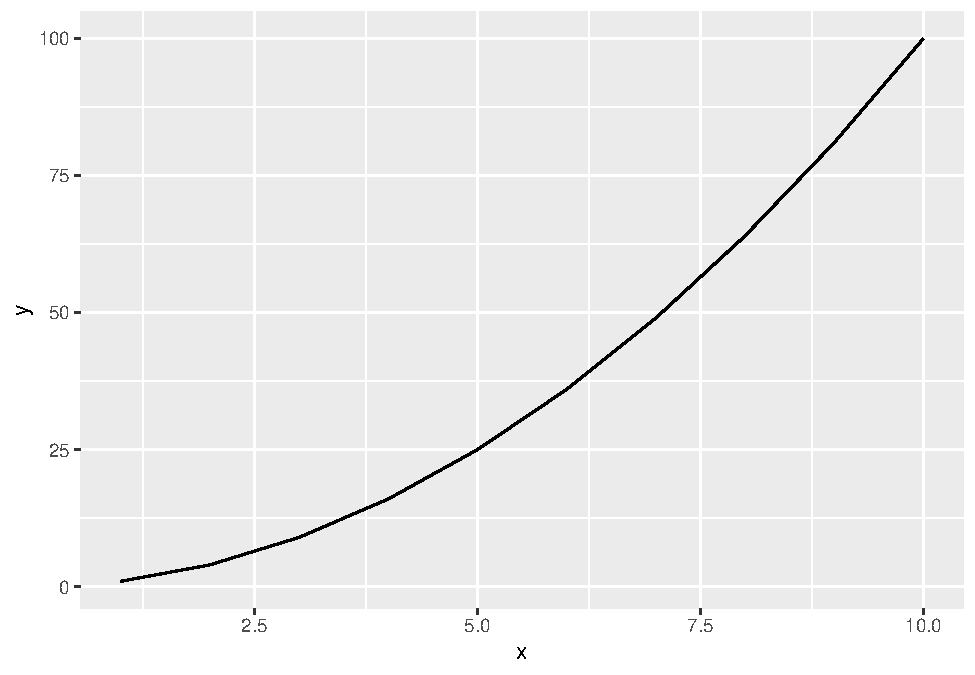
\includegraphics{People_Analytics_Lifecycle_files/figure-latex/unnamed-chunk-51-1.pdf}

Furthermore, we can use \texttt{ggplot} parameters and themes to adjust the aesthetics of visuals:

\begin{Shaded}
\begin{Highlighting}[]
\CommentTok{\# Produce line chart}
\NormalTok{ggplot2}\SpecialCharTok{::}\FunctionTok{ggplot}\NormalTok{(data, }\FunctionTok{aes}\NormalTok{(}\AttributeTok{x =}\NormalTok{ x, }\AttributeTok{y =}\NormalTok{ y)) }\SpecialCharTok{+}
\NormalTok{ggplot2}\SpecialCharTok{::}\FunctionTok{geom\_line}\NormalTok{(}\AttributeTok{size =}\NormalTok{ .}\DecValTok{4}\NormalTok{, }\AttributeTok{colour =} \StringTok{"blue"}\NormalTok{) }\SpecialCharTok{+} \CommentTok{\# Reduce line thickness and change color to blue}
\NormalTok{ggplot2}\SpecialCharTok{::}\FunctionTok{theme\_bw}\NormalTok{() }\SpecialCharTok{+} \CommentTok{\# Remove the default grey background}
\NormalTok{ggplot2}\SpecialCharTok{::}\FunctionTok{ggtitle}\NormalTok{(}\StringTok{"Plot Title }\SpecialCharTok{\textbackslash{}n}\StringTok{ Split between Two Lines"}\NormalTok{) }\SpecialCharTok{+} \CommentTok{\# Assign a title}
\NormalTok{ggplot2}\SpecialCharTok{::}\FunctionTok{xlab}\NormalTok{(}\StringTok{"Variable x Name"}\NormalTok{) }\SpecialCharTok{+} \CommentTok{\# Label the x{-}axis}
\NormalTok{ggplot2}\SpecialCharTok{::}\FunctionTok{ylab}\NormalTok{(}\StringTok{"Variable y Name"}\NormalTok{) }\SpecialCharTok{+} \CommentTok{\# Label the y{-}axis}
\NormalTok{ggplot2}\SpecialCharTok{::}\FunctionTok{theme}\NormalTok{(}\AttributeTok{plot.title =} \FunctionTok{element\_text}\NormalTok{(}\AttributeTok{hjust =} \FloatTok{0.5}\NormalTok{)) }\CommentTok{\# Center plot title}
\end{Highlighting}
\end{Shaded}

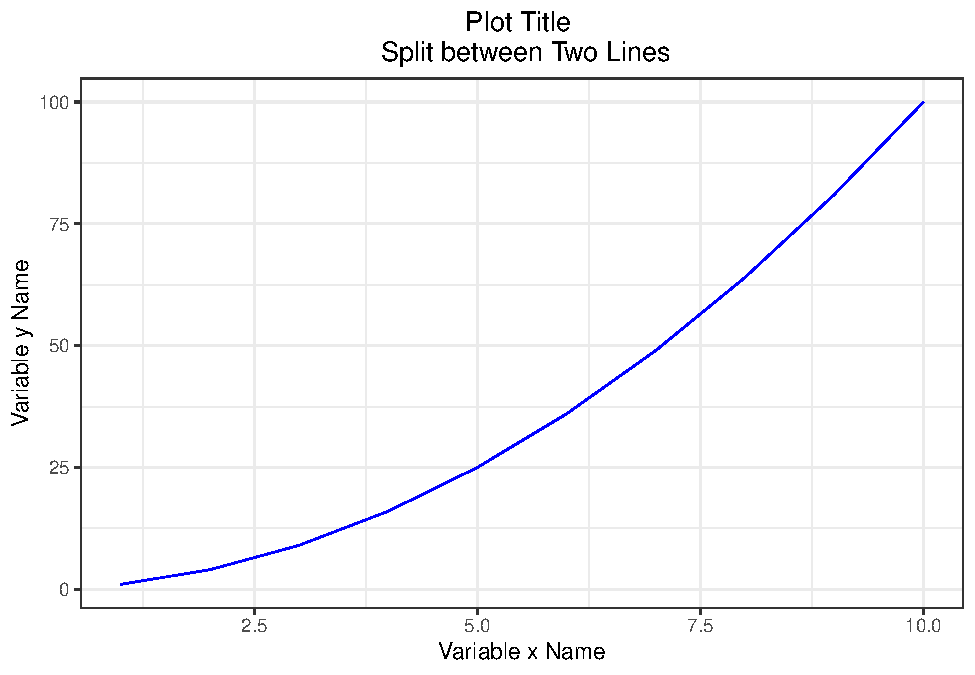
\includegraphics{People_Analytics_Lifecycle_files/figure-latex/unnamed-chunk-52-1.pdf}

\hypertarget{review-questions}{%
\section{Review Questions}\label{review-questions}}

\begin{enumerate}
\def\labelenumi{\arabic{enumi}.}
\item
  What is the difference between a factor and character vector?
\item
  What is vectorization?
\item
  How do data frames differ from matrices?
\item
  Does executing the \texttt{Sum()} function achieve the same result as executing \texttt{sum()}?
\item
  Does \texttt{seq(1,10)} return the same output as \texttt{1:10}?
\item
  Is the following command sufficient for creating a vector recognized by R as having three \emph{dates}: \texttt{dates\ \textless{}-\ c("2022-01-01",\ "2022-01-02",\ "2022-01-03")}.
\item
  How are \texttt{while} and \texttt{for} loops different?
\item
  If vectors \texttt{x1} and \texttt{x2} each hold 100 integers, how can we add each element of one to the respective element of the other using a single line of code?
\item
  How are slots in a list object referenced?
\item
  What are some examples in which a user-defined function (UDF) is needed?
\end{enumerate}

\hypertarget{sql-intro}{%
\chapter{Introduction to SQL}\label{sql-intro}}

\textbf{Structured Query Language (SQL)} is the most common language used to extract and wrangle data contained in a relational database. SQL is an essential skill for anyone working in analytics.

\hypertarget{basics}{%
\section{Basics}\label{basics}}

There are three main \emph{clauses} in a SQL query: (a) \texttt{SELECT}, (b) \texttt{FROM}, and (c) \texttt{WHERE}. The \texttt{SELECT} and \texttt{FROM} clauses are required, though the optional \texttt{WHERE} clause is frequently needed.

\begin{itemize}
\tightlist
\item
  \textbf{SELECT}: Specifies the columns to include in the output
\item
  \textbf{FROM}: Specifies the table(s) in which the relevant data are contained
\item
  \textbf{WHERE}: Specifies the rows to search
\end{itemize}

Despite the clauses being ordered as shown above (\texttt{SELECT} then \texttt{FROM} then \texttt{WHERE}), the \texttt{FROM} clause is the first to execute since we first need to identify the relevant table(s) before filtering rows and selecting columns. The \texttt{SELECT} clause is the last to execute.

Additional clauses are available for grouping and sorting data.

\begin{itemize}
\tightlist
\item
  \textbf{GROUP BY}: Specifies the columns by which data should be grouped when using aggregate functions
\item
  \textbf{HAVING}: Specifies conditions for filtering rows based on aggregate functions
\item
  \textbf{ORDER BY}: Specifies how data should be sorted in the output
\end{itemize}

When implementing aggregate functions in a \texttt{SELECT} clause, such as counting, summing, or averaging a numeric field, all other non-aggregated fields must be included in the \texttt{GROUP\ BY} clause.

When working with large datasets, it is best to filter records on the database side to avoid reading superfluous records into an analytics tool such as R only to then filter data to the relevant subset. For example, if we are performing an analysis on employees in the Engineering department, we should ideally filter to this subset on the database side rather than loading into R data on the entire workforce before paring down to the relevant records. Fewer records can help enhance the performance of R scripts -- especially when R is running on a local machine, such as a laptop, rather than on a more powerful server.

Though it is important to execute SQL queries directly on the database to minimize the amount of data read into R, we will use the \texttt{sqldf} library within R to demonstrate the mechanics of a SQL query for easily replicable examples. The \texttt{sqldf} library allows us to write SQL to query a data frame in R in lieu of a database. In a practical setting, we would pass a string containing the SQL query, execute it directly against the database, and then store the query's results to an object within R. While the syntax of SQL may vary by database, the core structure of queries is universal.

First, let's load the data sets:

\begin{Shaded}
\begin{Highlighting}[]
\CommentTok{\# Load data sets}
\NormalTok{employees }\OtherTok{\textless{}{-}} \FunctionTok{read.csv}\NormalTok{(}\StringTok{"/Users/craig.starbuck/Library/Mobile Documents/com\textasciitilde{}apple\textasciitilde{}CloudDocs/Documents/People Analytics Book/GitHub/peopleanalytics\_lifecycle\_book/data/employees.csv"}\NormalTok{)}
\NormalTok{status }\OtherTok{\textless{}{-}} \FunctionTok{read.csv}\NormalTok{(}\StringTok{"/Users/craig.starbuck/Library/Mobile Documents/com\textasciitilde{}apple\textasciitilde{}CloudDocs/Documents/People Analytics Book/GitHub/peopleanalytics\_lifecycle\_book/data/status.csv"}\NormalTok{)}
\NormalTok{benefits }\OtherTok{\textless{}{-}} \FunctionTok{read.csv}\NormalTok{(}\StringTok{"/Users/craig.starbuck/Library/Mobile Documents/com\textasciitilde{}apple\textasciitilde{}CloudDocs/Documents/People Analytics Book/GitHub/peopleanalytics\_lifecycle\_book/data/benefits.csv"}\NormalTok{)}
\NormalTok{demographics }\OtherTok{\textless{}{-}} \FunctionTok{read.csv}\NormalTok{(}\StringTok{"/Users/craig.starbuck/Library/Mobile Documents/com\textasciitilde{}apple\textasciitilde{}CloudDocs/Documents/People Analytics Book/GitHub/peopleanalytics\_lifecycle\_book/data/demographics.csv"}\NormalTok{)}
\NormalTok{job }\OtherTok{\textless{}{-}} \FunctionTok{read.csv}\NormalTok{(}\StringTok{"/Users/craig.starbuck/Library/Mobile Documents/com\textasciitilde{}apple\textasciitilde{}CloudDocs/Documents/People Analytics Book/GitHub/peopleanalytics\_lifecycle\_book/data/job.csv"}\NormalTok{)}
\NormalTok{payroll }\OtherTok{\textless{}{-}} \FunctionTok{read.csv}\NormalTok{(}\StringTok{"/Users/craig.starbuck/Library/Mobile Documents/com\textasciitilde{}apple\textasciitilde{}CloudDocs/Documents/People Analytics Book/GitHub/peopleanalytics\_lifecycle\_book/data/payroll.csv"}\NormalTok{)}
\NormalTok{performance }\OtherTok{\textless{}{-}} \FunctionTok{read.csv}\NormalTok{(}\StringTok{"/Users/craig.starbuck/Library/Mobile Documents/com\textasciitilde{}apple\textasciitilde{}CloudDocs/Documents/People Analytics Book/GitHub/peopleanalytics\_lifecycle\_book/data/performance.csv"}\NormalTok{)}
\NormalTok{prior\_employment }\OtherTok{\textless{}{-}} \FunctionTok{read.csv}\NormalTok{(}\StringTok{"/Users/craig.starbuck/Library/Mobile Documents/com\textasciitilde{}apple\textasciitilde{}CloudDocs/Documents/People Analytics Book/GitHub/peopleanalytics\_lifecycle\_book/data/prior\_employment.csv"}\NormalTok{)}
\NormalTok{survey\_response }\OtherTok{\textless{}{-}} \FunctionTok{read.csv}\NormalTok{(}\StringTok{"/Users/craig.starbuck/Library/Mobile Documents/com\textasciitilde{}apple\textasciitilde{}CloudDocs/Documents/People Analytics Book/GitHub/peopleanalytics\_lifecycle\_book/data/survey\_response.csv"}\NormalTok{)}
\NormalTok{tenure }\OtherTok{\textless{}{-}} \FunctionTok{read.csv}\NormalTok{(}\StringTok{"/Users/craig.starbuck/Library/Mobile Documents/com\textasciitilde{}apple\textasciitilde{}CloudDocs/Documents/People Analytics Book/GitHub/peopleanalytics\_lifecycle\_book/data/tenure.csv"}\NormalTok{)}

\CommentTok{\# Return row and column counts}
\FunctionTok{dim}\NormalTok{(employees)}
\end{Highlighting}
\end{Shaded}

\begin{verbatim}
## [1] 1470   36
\end{verbatim}

Next, we will apply the \texttt{sqldf()} function to our data frame to extract specific rows and columns. In addition to the \texttt{SELECT}, \texttt{FROM}, and \texttt{WHERE} clauses, we will use the \texttt{LIMIT} clause to limit the number of rows that are displayed given the data frame's size (\(n = 1,470\)). In a practical setting, the \texttt{LIMIT} clause is only used for efficient data profiling and troubleshooting, as we would not want to arbitrarily truncate a data set used for analysis.

A best practice in writing SQL is to capitalize the names of clauses and functions and to use separate lines and indentation to make the SQL statements more readable:

\begin{Shaded}
\begin{Highlighting}[]
\CommentTok{\# Load SQL library}
\FunctionTok{library}\NormalTok{(sqldf)}

\CommentTok{\# Store SQL query as a character string using the paste() function}
\NormalTok{sql\_string }\OtherTok{\textless{}{-}} \FunctionTok{paste}\NormalTok{(}\StringTok{"SELECT}
\StringTok{                      employee\_id}
\StringTok{                    FROM}
\StringTok{                      employees}
\StringTok{                    WHERE}
\StringTok{                      dept = \textquotesingle{}Research \& Development\textquotesingle{}}
\StringTok{                    LIMIT 10"}\NormalTok{)}

\CommentTok{\# Execute SQL query}
\NormalTok{sqldf}\SpecialCharTok{::}\FunctionTok{sqldf}\NormalTok{(sql\_string)}
\end{Highlighting}
\end{Shaded}

\begin{verbatim}
##    employee_id
## 1         1002
## 2         1003
## 3         1004
## 4         1005
## 5         1006
## 6         1007
## 7         1008
## 8         1009
## 9         1010
## 10        1011
\end{verbatim}

This query returned a list of employee ids for employees in the Research \& Development department.

To optimize query performance, it is important to order conditions in the \texttt{WHERE} clause beginning with the condition that will exclude the largest number of records. Conditions are executed sequentially, and each subsequent condition must evaluate all records that remain following any preceding filtering. Limiting the number of records that must be searched when evaluating each condition will reduce the time it takes the query to return results. For example, if two conditions are needed and one excludes 5,000 records while the other excludes 10, the condition that excludes 5,000 records should be listed first in the \texttt{WHERE} clause.

\hypertarget{aggregate-functions}{%
\section{Aggregate Functions}\label{aggregate-functions}}

Next, let's take a look at average organization tenure by job for those in the Research \& Development department:

\begin{Shaded}
\begin{Highlighting}[]
\CommentTok{\# Store SQL query as a character string}
\NormalTok{sql\_string }\OtherTok{\textless{}{-}} \FunctionTok{paste}\NormalTok{(}\StringTok{"SELECT}
\StringTok{                      job\_title,}
\StringTok{                      AVG(org\_tenure)}
\StringTok{                    FROM}
\StringTok{                      employees}
\StringTok{                    WHERE}
\StringTok{                      dept = \textquotesingle{}Research \& Development\textquotesingle{}}
\StringTok{                    GROUP BY}
\StringTok{                      job\_title"}\NormalTok{)}

\CommentTok{\# Execute SQL query}
\NormalTok{sqldf}\SpecialCharTok{::}\FunctionTok{sqldf}\NormalTok{(sql\_string)}
\end{Highlighting}
\end{Shaded}

\begin{verbatim}
##                   job_title AVG(org_tenure)
## 1 Healthcare Representative        8.618321
## 2     Laboratory Technician        5.019305
## 3                   Manager       13.673077
## 4    Manufacturing Director        7.600000
## 5         Research Director       10.937500
## 6        Research Scientist        5.113014
## 7            Vice President        9.500000
\end{verbatim}

There are 7 distinct job titles among employees in the Research \& Development department, and the average organization tenure for these ranges from \texttt{5} to \texttt{13.7} years.

Since there could be a small number of employees in certain jobs, in which case average organization tenure may not be as meaningful, we can use the \texttt{COUNT(*)} function to count the number of rows for each group. In this case, \texttt{COUNT(*)} will return the number of employees in each job in the Research \& Development department. We will also apply column aliases via \texttt{AS} in the \texttt{SELECT} clause to assign different names to the output fields:

\begin{Shaded}
\begin{Highlighting}[]
\CommentTok{\# Store SQL query as a character string}
\NormalTok{sql\_string }\OtherTok{\textless{}{-}} \FunctionTok{paste}\NormalTok{(}\StringTok{"SELECT}
\StringTok{                      job\_title,}
\StringTok{                      COUNT(*) AS employee\_cnt,}
\StringTok{                      AVG(org\_tenure) AS avg\_org\_tenure}
\StringTok{                    FROM}
\StringTok{                      employees}
\StringTok{                    WHERE}
\StringTok{                      dept = \textquotesingle{}Research \& Development\textquotesingle{}}
\StringTok{                    GROUP BY}
\StringTok{                      job\_title}
\StringTok{                    ORDER BY}
\StringTok{                      job\_title"}\NormalTok{)}

\CommentTok{\# Execute SQL query}
\NormalTok{sqldf}\SpecialCharTok{::}\FunctionTok{sqldf}\NormalTok{(sql\_string)}
\end{Highlighting}
\end{Shaded}

\begin{verbatim}
##                   job_title employee_cnt avg_org_tenure
## 1 Healthcare Representative          131       8.618321
## 2     Laboratory Technician          259       5.019305
## 3                   Manager           52      13.673077
## 4    Manufacturing Director          145       7.600000
## 5         Research Director           80      10.937500
## 6        Research Scientist          292       5.113014
## 7            Vice President            2       9.500000
\end{verbatim}

The output shows that there are only 2 Vice Presidents in the Research \& Development department, while other job titles are much more prevalent.

Since relatively few employees are Vice Presidents, let's use the \texttt{HAVING} clause to only show average organization tenure for Research \& Development department jobs with more than 10 employees. We can also use the \texttt{ROUND()} function to truncate average organization tenure to one significant digit:

\begin{Shaded}
\begin{Highlighting}[]
\CommentTok{\# Store SQL query as a character string}
\NormalTok{sql\_string }\OtherTok{\textless{}{-}} \FunctionTok{paste}\NormalTok{(}\StringTok{"SELECT}
\StringTok{                      job\_title,}
\StringTok{                      COUNT(*) AS employee\_cnt,}
\StringTok{                      ROUND(AVG(org\_tenure), 1) AS avg\_org\_tenure}
\StringTok{                    FROM}
\StringTok{                      employees}
\StringTok{                    WHERE}
\StringTok{                      dept = \textquotesingle{}Research \& Development\textquotesingle{}}
\StringTok{                    GROUP BY}
\StringTok{                      job\_title}
\StringTok{                    HAVING}
\StringTok{                      COUNT(*) \textgreater{} 10}
\StringTok{                    ORDER BY}
\StringTok{                      job\_title"}\NormalTok{)}

\CommentTok{\# Execute SQL query}
\NormalTok{sqldf}\SpecialCharTok{::}\FunctionTok{sqldf}\NormalTok{(sql\_string)}
\end{Highlighting}
\end{Shaded}

\begin{verbatim}
##                   job_title employee_cnt avg_org_tenure
## 1 Healthcare Representative          131            8.6
## 2     Laboratory Technician          259            5.0
## 3                   Manager           52           13.7
## 4    Manufacturing Director          145            7.6
## 5         Research Director           80           10.9
## 6        Research Scientist          292            5.1
\end{verbatim}

\hypertarget{joins}{%
\section{Joins}\label{joins}}

In a practical setting, the required data are rarely contained within a single table. Therefore, we must query multiple tables and join them together. Figure \ref{fig:sql-joins} illustrates SQL join types using Venn diagrams:

\begin{figure}

{\centering 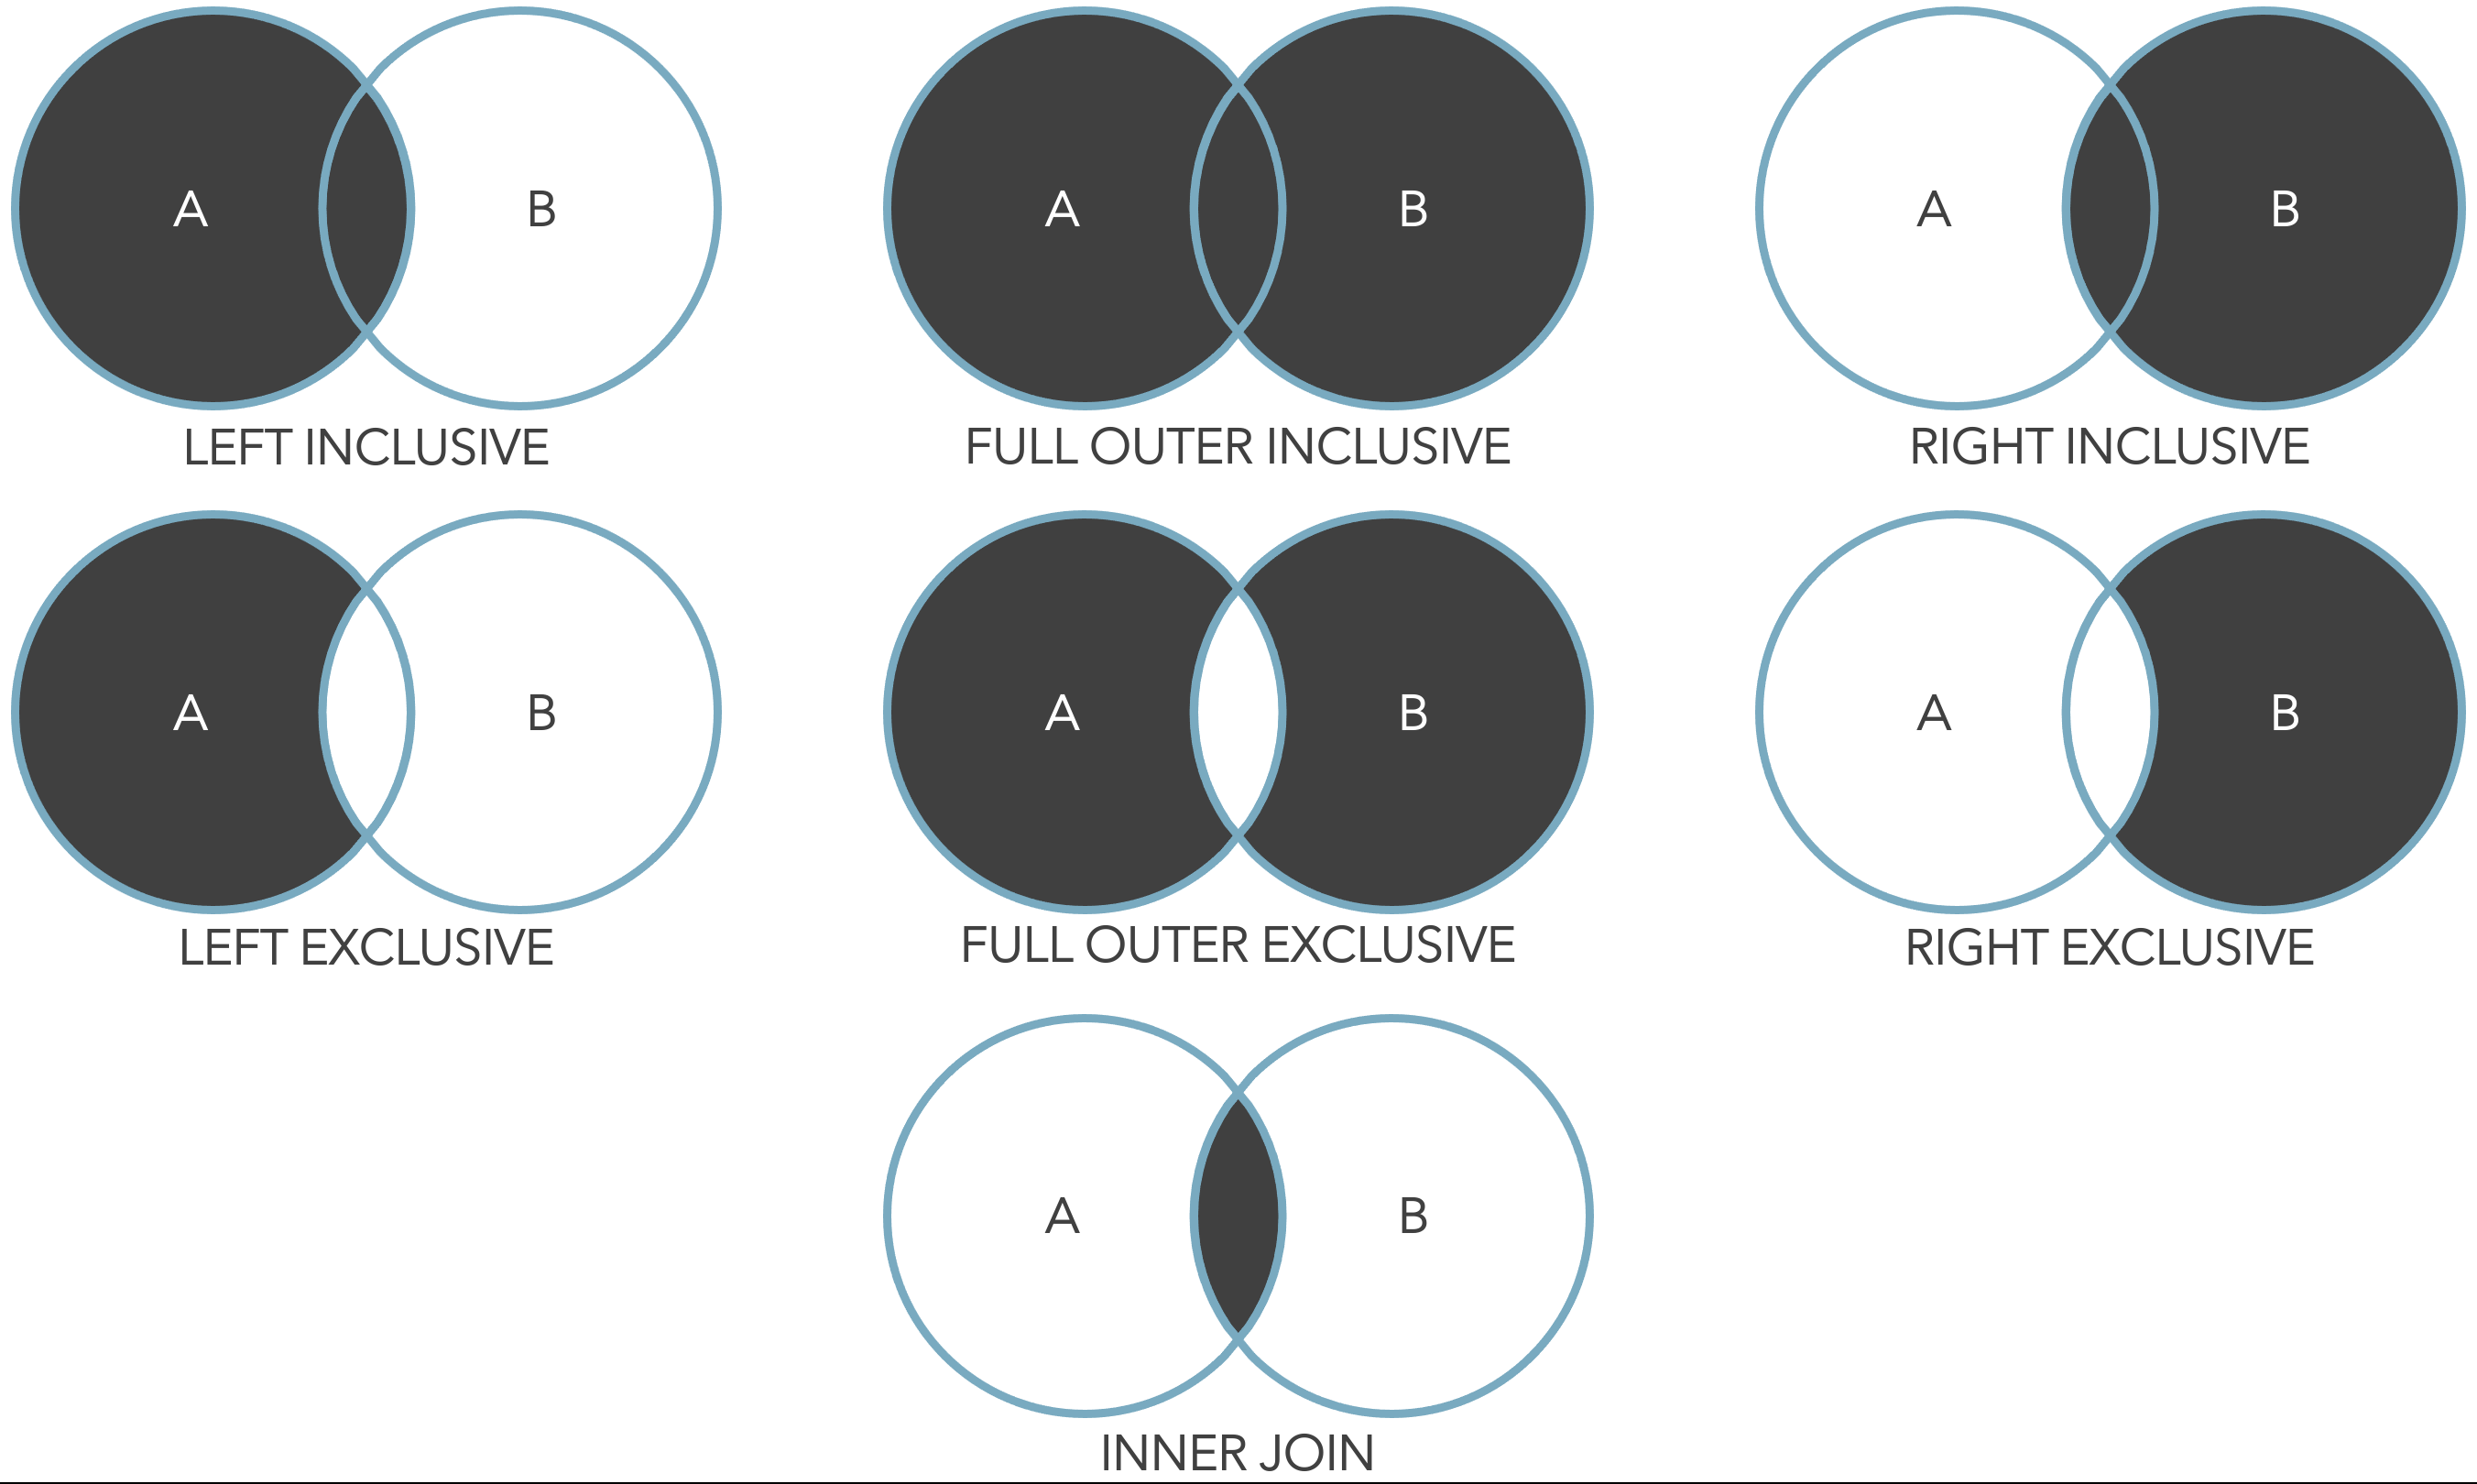
\includegraphics[width=1\linewidth]{/Users/craig.starbuck/Library/Mobile Documents/com~apple~CloudDocs/Documents/People Analytics Book/GitHub/peopleanalytics_lifecycle_book/graphics/sql_joins} 

}

\caption{Types of SQL Joins}\label{fig:sql-joins}
\end{figure}

The structure of SQL queries containing each type of join is represented below:

\textbf{LEFT INCLUSIVE}

\begin{Shaded}
\begin{Highlighting}[]
\CommentTok{\#  SELECT [Output Field List]}
\CommentTok{\#  FROM A }
\CommentTok{\#  LEFT OUTER JOIN B}
\CommentTok{\#  ON A.Key = B.Key}
\end{Highlighting}
\end{Shaded}

\textbf{LEFT EXCLUSIVE}

\begin{Shaded}
\begin{Highlighting}[]
\CommentTok{\#  SELECT [Output Field List]}
\CommentTok{\#  FROM A }
\CommentTok{\#  LEFT OUTER JOIN B}
\CommentTok{\#  ON A.Key = B.Key}
\CommentTok{\#  WHERE B.Key IS NULL}
\end{Highlighting}
\end{Shaded}

\textbf{FULL OUTER INCLUSIVE}

\begin{Shaded}
\begin{Highlighting}[]
\CommentTok{\#  SELECT [Output Field List]}
\CommentTok{\#  FROM A }
\CommentTok{\#  FULL OUTER JOIN B}
\CommentTok{\#  ON A.Key = B.Key}
\end{Highlighting}
\end{Shaded}

\textbf{FULL OUTER EXCLUSIVE}

\begin{Shaded}
\begin{Highlighting}[]
\CommentTok{\#  SELECT [Output Field List]}
\CommentTok{\#  FROM A }
\CommentTok{\#  FULL OUTER JOIN B}
\CommentTok{\#  ON A.Key = B.Key}
\CommentTok{\#  WHERE A.Key IS NULL OR B.Key IS NULL  }
\end{Highlighting}
\end{Shaded}

\textbf{RIGHT INCLUSIVE}

\begin{Shaded}
\begin{Highlighting}[]
\CommentTok{\#  SELECT [Output Field List]}
\CommentTok{\#  FROM A }
\CommentTok{\#  RIGHT OUTER JOIN B}
\CommentTok{\#  ON A.Key = B.Key}
\end{Highlighting}
\end{Shaded}

\textbf{RIGHT EXCLUSIVE}

\begin{Shaded}
\begin{Highlighting}[]
\CommentTok{\#  SELECT [Output Field List]}
\CommentTok{\#  FROM A }
\CommentTok{\#  LEFT OUTER JOIN B}
\CommentTok{\#  ON A.Key = B.Key}
\CommentTok{\#  WHERE A.Key IS NULL}
\end{Highlighting}
\end{Shaded}

\textbf{INNER JOIN}

\begin{Shaded}
\begin{Highlighting}[]
\CommentTok{\#  SELECT [Output Field List]}
\CommentTok{\#  FROM A }
\CommentTok{\#  INNER JOIN B}
\CommentTok{\#  ON A.Key = B.Key}
\end{Highlighting}
\end{Shaded}

To illustrate how SQL joins work, we will leverage three of the data sets used to produce the consolidated \texttt{employees} data set we have been using: \texttt{job}, \texttt{tenure}, and \texttt{demographics}. For many people analytics projects, employee id is the PK since this identifier for one employee should not be assigned to another employee -- past, present, or future. Email or network id may also be a suitable PK. We will use the \texttt{employee\_id} column in each of the three data frames to facilitate joins:

Next, we will query these data frames to return the average organization tenure and average commute distance for employees in the Research \& Development department, grouped by jobs with more than 10 employees. For this, we will leverage an \texttt{INNER\ JOIN}, which will return records only for employee ids which are present in all three data frames. For example, if a record exists in \texttt{demographics} and \texttt{tenure} for a particular employee id, but there is no corresponding record in \texttt{job}, that employee id would not be included in the output.

\begin{Shaded}
\begin{Highlighting}[]
\CommentTok{\# Store SQL query as a character string}
\NormalTok{sql\_string }\OtherTok{\textless{}{-}} \FunctionTok{paste}\NormalTok{(}\StringTok{"SELECT}
\StringTok{                      job\_title,}
\StringTok{                      COUNT(*) AS employee\_cnt,}
\StringTok{                      ROUND(AVG(org\_tenure), 1) AS avg\_org\_tenure,}
\StringTok{                      ROUND(AVG(commute\_dist), 1) AS avg\_commute\_dist}
\StringTok{                    FROM}
\StringTok{                        demographics}
\StringTok{                      INNER JOIN}
\StringTok{                        tenure}
\StringTok{                      ON}
\StringTok{                        demographics.employee\_id = tenure.employee\_id}
\StringTok{                      INNER JOIN}
\StringTok{                        job}
\StringTok{                      ON}
\StringTok{                        demographics.employee\_id = job.employee\_id}
\StringTok{                    WHERE}
\StringTok{                      dept = \textquotesingle{}Research \& Development\textquotesingle{}}
\StringTok{                    GROUP BY}
\StringTok{                      job\_title}
\StringTok{                    HAVING}
\StringTok{                      COUNT(*) \textgreater{} 10}
\StringTok{                    ORDER BY}
\StringTok{                      job\_title"}\NormalTok{)}

\CommentTok{\# Execute SQL query}
\NormalTok{sqldf}\SpecialCharTok{::}\FunctionTok{sqldf}\NormalTok{(sql\_string)}
\end{Highlighting}
\end{Shaded}

\begin{verbatim}
##                   job_title employee_cnt avg_org_tenure avg_commute_dist
## 1 Healthcare Representative          131            8.6              9.8
## 2     Laboratory Technician          259            5.0              9.4
## 3                   Manager           52           13.7              7.2
## 4    Manufacturing Director          145            7.6              9.5
## 5         Research Director           80           10.9              8.4
## 6        Research Scientist          292            5.1              9.0
\end{verbatim}

Note that the \texttt{INNER\ JOIN} in this SQL query was structured such that both \texttt{tenure} and \texttt{job} were joined to \texttt{demographics} via the \texttt{employee\_id} column. We could have instead joined \texttt{job} to \texttt{tenure} since we joined \texttt{tenure} to \texttt{demographics}; this would have achieved the same result since all employee ids exist in each of the three data frames.

If it were possible for all employee ids to exist in \texttt{demographics} but not in either \texttt{tenure} or \texttt{job}, we could leverage a \texttt{LEFT\ JOIN} to ensure all records from \texttt{demographics} are included in the output irrespective of whether they have matches in \texttt{tenure} or \texttt{job}:

\begin{Shaded}
\begin{Highlighting}[]
\CommentTok{\# Store SQL query as a character string}
\NormalTok{sql\_string }\OtherTok{\textless{}{-}} \FunctionTok{paste}\NormalTok{(}\StringTok{"SELECT}
\StringTok{                      job\_title,}
\StringTok{                      COUNT(*) AS employee\_cnt,}
\StringTok{                      ROUND(AVG(org\_tenure), 1) AS avg\_org\_tenure,}
\StringTok{                      ROUND(AVG(commute\_dist), 1) AS avg\_commute\_dist}
\StringTok{                    FROM}
\StringTok{                        demographics}
\StringTok{                      LEFT JOIN}
\StringTok{                        tenure}
\StringTok{                      ON}
\StringTok{                        demographics.employee\_id = tenure.employee\_id}
\StringTok{                      LEFT JOIN}
\StringTok{                        job}
\StringTok{                      ON}
\StringTok{                        demographics.employee\_id = job.employee\_id}
\StringTok{                    WHERE}
\StringTok{                      dept = \textquotesingle{}Research \& Development\textquotesingle{}}
\StringTok{                    GROUP BY}
\StringTok{                      job\_title}
\StringTok{                    HAVING}
\StringTok{                      COUNT(*) \textgreater{} 10}
\StringTok{                    ORDER BY}
\StringTok{                      job\_title"}\NormalTok{)}

\CommentTok{\# Execute SQL query}
\NormalTok{sqldf}\SpecialCharTok{::}\FunctionTok{sqldf}\NormalTok{(sql\_string)}
\end{Highlighting}
\end{Shaded}

\begin{verbatim}
##                   job_title employee_cnt avg_org_tenure avg_commute_dist
## 1 Healthcare Representative          131            8.6              9.8
## 2     Laboratory Technician          259            5.0              9.4
## 3                   Manager           52           13.7              7.2
## 4    Manufacturing Director          145            7.6              9.5
## 5         Research Director           80           10.9              8.4
## 6        Research Scientist          292            5.1              9.0
\end{verbatim}

In this case, if demographics is the base data set which contains all employee ids (i.e., the `LEFT' dataset), it is important for \texttt{tenure} and \texttt{job} to be joined to it. Joining \texttt{job} to \texttt{tenure} may result in information loss if an employee id exists in \texttt{demographics} and \texttt{job} but not in the intermediate \texttt{tenure} data set.

When integrating data within R, the \texttt{tidyverse} provides a more efficient and parsimonious method of joining many data sets using various join types. Within this framework, components are chained together via the package-specific \texttt{\%\textgreater{}\%} operator. The example below joins nine data sets into a single \texttt{employees} data frame using a left join on the \texttt{employee\_id} column:

\begin{Shaded}
\begin{Highlighting}[]
\CommentTok{\# Load tidyverse}
\FunctionTok{library}\NormalTok{(tidyverse)}

\NormalTok{employees }\OtherTok{\textless{}{-}} \FunctionTok{list}\NormalTok{(demographics,}
\NormalTok{                  status,}
\NormalTok{                  benefits,}
\NormalTok{                  job,}
\NormalTok{                  payroll,}
\NormalTok{                  performance,}
\NormalTok{                  prior\_employment,}
\NormalTok{                  survey\_response,}
\NormalTok{                  tenure) }\SpecialCharTok{\%\textgreater{}\%}
                  \FunctionTok{reduce}\NormalTok{(left\_join, }\AttributeTok{by =} \StringTok{"employee\_id"}\NormalTok{)}
\end{Highlighting}
\end{Shaded}

\hypertarget{subqueries}{%
\section{Subqueries}\label{subqueries}}

\textbf{Subqueries} are queries nested within other queries. Subqueries are often referred to as \textbf{inner queries}, while the main queries are referred to as \textbf{outer queries}.

For example, if we are interested in performing an analysis on employees with more than a year of organization tenure, we can use a subquery to pass a list of employee ids that meet this criterion into the outer query for filtering. In this case, we would not need to include \texttt{tenure} in the join conditions of our main query:

\begin{Shaded}
\begin{Highlighting}[]
\CommentTok{\# Store SQL query as a character string}
\CommentTok{\# Note: Since employee\_id exists in multiple data sets, we must name a specific data set when referencing it}
\NormalTok{sql\_string }\OtherTok{\textless{}{-}} \FunctionTok{paste}\NormalTok{(}\StringTok{"SELECT}
\StringTok{                      job\_title,}
\StringTok{                      COUNT(*) AS employee\_cnt,}
\StringTok{                      ROUND(AVG(commute\_dist), 1) AS avg\_commute\_dist}
\StringTok{                    FROM}
\StringTok{                        demographics}
\StringTok{                      LEFT JOIN}
\StringTok{                        job}
\StringTok{                      ON}
\StringTok{                        demographics.employee\_id = job.employee\_id}
\StringTok{                    WHERE}
\StringTok{                        demographics.employee\_id IN (SELECT employee\_id FROM tenure WHERE org\_tenure \textgreater{} 1)}
\StringTok{                      AND }
\StringTok{                        dept = \textquotesingle{}Research \& Development\textquotesingle{}}
\StringTok{                    GROUP BY}
\StringTok{                      job\_title}
\StringTok{                    HAVING}
\StringTok{                      COUNT(*) \textgreater{} 10}
\StringTok{                    ORDER BY}
\StringTok{                      job\_title"}\NormalTok{)}

\CommentTok{\# Execute SQL query}
\NormalTok{sqldf}\SpecialCharTok{::}\FunctionTok{sqldf}\NormalTok{(sql\_string)}
\end{Highlighting}
\end{Shaded}

\begin{verbatim}
##                   job_title employee_cnt avg_commute_dist
## 1 Healthcare Representative          118              9.7
## 2     Laboratory Technician          198              9.6
## 3                   Manager           49              6.9
## 4    Manufacturing Director          133              9.7
## 5         Research Director           74              8.3
## 6        Research Scientist          238              9.2
\end{verbatim}

\hypertarget{virtual-tables}{%
\section{Virtual Tables}\label{virtual-tables}}

An alternative to a subquery is creating a \textbf{virtual table} in the \texttt{FROM} clause. When using an \texttt{INNER\ JOIN} to connect \texttt{demographics} to the virtual table \texttt{ids}, which provides a list of employee ids for those with more than a year of organization tenure, any records in \texttt{demographics} or \texttt{job} that do not relate to employees with at least a year of organization tenure will be dropped. This is true even though a \texttt{LEFT\ JOIN} is used to join \texttt{job} to \texttt{demographics} since records in \texttt{demographics} will be filtered based on \texttt{employee\_id} matches in the virtual table. With this approach, our \texttt{WHERE} clause is limited to the \texttt{department\ =\ \textquotesingle{}Research\ \&\ Development\textquotesingle{}} condition:

\begin{Shaded}
\begin{Highlighting}[]
\CommentTok{\# Store SQL query as a character string}
\NormalTok{sql\_string }\OtherTok{\textless{}{-}} \FunctionTok{paste}\NormalTok{(}\StringTok{"SELECT}
\StringTok{                      job\_title,}
\StringTok{                      COUNT(*) AS employee\_cnt,}
\StringTok{                      ROUND(AVG(commute\_dist), 1) AS avg\_commute\_dist}
\StringTok{                    FROM}
\StringTok{                        demographics}
\StringTok{                      LEFT JOIN}
\StringTok{                        job}
\StringTok{                      ON}
\StringTok{                        demographics.employee\_id = job.employee\_id}
\StringTok{                      INNER JOIN}
\StringTok{                        (SELECT employee\_id FROM tenure WHERE org\_tenure \textgreater{} 1) ids}
\StringTok{                      ON}
\StringTok{                        demographics.employee\_id = ids.employee\_id}
\StringTok{                    WHERE}
\StringTok{                      dept = \textquotesingle{}Research \& Development\textquotesingle{}}
\StringTok{                    GROUP BY}
\StringTok{                      job\_title}
\StringTok{                    HAVING}
\StringTok{                      COUNT(*) \textgreater{} 10}
\StringTok{                    ORDER BY}
\StringTok{                      job\_title"}\NormalTok{)}

\CommentTok{\# Execute SQL query}
\NormalTok{sqldf}\SpecialCharTok{::}\FunctionTok{sqldf}\NormalTok{(sql\_string)}
\end{Highlighting}
\end{Shaded}

\begin{verbatim}
##                   job_title employee_cnt avg_commute_dist
## 1 Healthcare Representative          118              9.7
## 2     Laboratory Technician          198              9.6
## 3                   Manager           49              6.9
## 4    Manufacturing Director          133              9.7
## 5         Research Director           74              8.3
## 6        Research Scientist          238              9.2
\end{verbatim}

As you can see, the output of the query using a virtual table matches the results from the preceding approach that utilized a subquery.

\hypertarget{window-functions}{%
\section{Window Functions}\label{window-functions}}

\textbf{Window functions} are used for performing calculations over a set of rows without collapsing the records. Unlike the aggregate functions we've covered, window functions do not collapse rows into a single value; the calculated value is returned for each of the rows over which the calculation is performed.

For example, we can assign an organization tenure rank by Research \& Development job using the \texttt{RANK()} and \texttt{OVER()} functions in the \texttt{SELECT} clause. The \texttt{PARTITION\ BY} argument functions like a \texttt{GROUP\ BY} clause but without collapsing rows, while the \texttt{ORDER\ BY} argument sorts the records in ascending (\texttt{ASC}) or descending (\texttt{DESC}) order for proper ranking:

\begin{Shaded}
\begin{Highlighting}[]
\CommentTok{\# Store SQL query as a character string}
\CommentTok{\# Limit output to 10 records since query does not collapse records}
\NormalTok{sql\_string }\OtherTok{\textless{}{-}} \FunctionTok{paste}\NormalTok{(}\StringTok{"SELECT}
\StringTok{                      demographics.employee\_id,}
\StringTok{                      job\_title,}
\StringTok{                      commute\_dist,}
\StringTok{                      RANK () OVER (PARTITION BY job\_title ORDER BY commute\_dist DESC) AS commute\_dist\_rank}
\StringTok{                    FROM}
\StringTok{                        demographics}
\StringTok{                      LEFT JOIN}
\StringTok{                        job}
\StringTok{                      ON}
\StringTok{                        demographics.employee\_id = job.employee\_id}
\StringTok{                      INNER JOIN}
\StringTok{                        (SELECT employee\_id FROM tenure WHERE org\_tenure \textgreater{} 1) ids}
\StringTok{                      ON}
\StringTok{                        demographics.employee\_id = ids.employee\_id}
\StringTok{                    WHERE}
\StringTok{                      dept = \textquotesingle{}Research \& Development\textquotesingle{}}
\StringTok{                    ORDER BY}
\StringTok{                      job\_title,}
\StringTok{                      commute\_dist\_rank}
\StringTok{                    LIMIT 10"}\NormalTok{)}

\CommentTok{\# Execute SQL query}
\NormalTok{sqldf}\SpecialCharTok{::}\FunctionTok{sqldf}\NormalTok{(sql\_string)}
\end{Highlighting}
\end{Shaded}

\begin{verbatim}
##    employee_id                 job_title commute_dist commute_dist_rank
## 1         2325 Healthcare Representative           29                 1
## 2         1414 Healthcare Representative           28                 2
## 3         1010 Healthcare Representative           27                 3
## 4         1573 Healthcare Representative           27                 3
## 5         2200 Healthcare Representative           26                 5
## 6         1730 Healthcare Representative           25                 6
## 7         1833 Healthcare Representative           25                 6
## 8         1993 Healthcare Representative           25                 6
## 9         2415 Healthcare Representative           25                 6
## 10        1164 Healthcare Representative           24                10
\end{verbatim}

Notice that in the case of commute distance ties, the \texttt{RANK()} function assigns the same rank and then adds the number of ties to that rank to determine the rank for the next highest value of commute distance.

We can also treat this query as a virtual table, and then filter on the derived \texttt{commute\_dist\_rank} field to return the highest commute distance for each job. We can add a \texttt{DISTINCT()} function in the \texttt{SELECT} clause to collapse jobs for which there are more than one employee with the max commute distance, and display the number of ties for each using the \texttt{COUNT(*)} function:

\begin{Shaded}
\begin{Highlighting}[]
\CommentTok{\# Store SQL query as a character string}
\NormalTok{sql\_string }\OtherTok{\textless{}{-}} \FunctionTok{paste}\NormalTok{(}\StringTok{"SELECT}
\StringTok{                        DISTINCT(job\_title) AS job\_title,}
\StringTok{                        COUNT(*) AS employee\_count,}
\StringTok{                        commute\_dist}
\StringTok{                     FROM}
\StringTok{                        (SELECT}
\StringTok{                          demographics.employee\_id,}
\StringTok{                          job\_title,}
\StringTok{                          commute\_dist,}
\StringTok{                          RANK () OVER (PARTITION BY job\_title ORDER BY commute\_dist DESC) AS commute\_dist\_rank}
\StringTok{                        FROM}
\StringTok{                            demographics}
\StringTok{                          LEFT JOIN}
\StringTok{                            job}
\StringTok{                          ON}
\StringTok{                            demographics.employee\_id = job.employee\_id}
\StringTok{                          INNER JOIN}
\StringTok{                            (SELECT employee\_id FROM tenure WHERE org\_tenure \textgreater{} 1) ids}
\StringTok{                          ON}
\StringTok{                            demographics.employee\_id = ids.employee\_id}
\StringTok{                        WHERE}
\StringTok{                          dept = \textquotesingle{}Research \& Development\textquotesingle{}}
\StringTok{                        ORDER BY}
\StringTok{                          job\_title,}
\StringTok{                          commute\_dist\_rank) tbl}
\StringTok{                      WHERE}
\StringTok{                        tbl.commute\_dist\_rank = 1}
\StringTok{                      GROUP BY}
\StringTok{                        job\_title"}\NormalTok{)}

\CommentTok{\# Execute SQL query}
\NormalTok{sqldf}\SpecialCharTok{::}\FunctionTok{sqldf}\NormalTok{(sql\_string)}
\end{Highlighting}
\end{Shaded}

\begin{verbatim}
##                   job_title employee_count commute_dist
## 1 Healthcare Representative              1           29
## 2     Laboratory Technician              6           29
## 3                   Manager              2           29
## 4    Manufacturing Director              4           29
## 5         Research Director              3           28
## 6        Research Scientist              4           29
## 7            Vice President              1            8
\end{verbatim}

\hypertarget{common-table-expressions-ctes}{%
\section{Common Table Expressions (CTEs)}\label{common-table-expressions-ctes}}

An alternative approach is to use a \textbf{common table expression (CTE)}, which is the result set of a query that exists temporarily and only for use in a larger query. Like the virtual table example, CTEs do not persist data in objects or tables; the data exist only for the duration of the query.

\begin{Shaded}
\begin{Highlighting}[]
\CommentTok{\# Store SQL query as a character string}
\NormalTok{sql\_string }\OtherTok{\textless{}{-}} \FunctionTok{paste}\NormalTok{(}\StringTok{"WITH max\_commute\_job}
\StringTok{                     AS}
\StringTok{                        (SELECT}
\StringTok{                          demographics.employee\_id,}
\StringTok{                          job\_title,}
\StringTok{                          commute\_dist,}
\StringTok{                          RANK () OVER (PARTITION BY job\_title ORDER BY commute\_dist DESC) AS commute\_dist\_rank}
\StringTok{                        FROM}
\StringTok{                            demographics}
\StringTok{                          LEFT JOIN}
\StringTok{                            job}
\StringTok{                          ON}
\StringTok{                            demographics.employee\_id = job.employee\_id}
\StringTok{                          INNER JOIN}
\StringTok{                            (SELECT employee\_id FROM tenure WHERE org\_tenure \textgreater{} 1) ids}
\StringTok{                          ON}
\StringTok{                            demographics.employee\_id = ids.employee\_id}
\StringTok{                        WHERE}
\StringTok{                          dept = \textquotesingle{}Research \& Development\textquotesingle{}}
\StringTok{                        ORDER BY}
\StringTok{                          job\_title,}
\StringTok{                          commute\_dist\_rank)}
\StringTok{                      }
\StringTok{                      SELECT}
\StringTok{                        DISTINCT(job\_title) AS job\_title,}
\StringTok{                        COUNT(*) AS employee\_count,}
\StringTok{                        commute\_dist}
\StringTok{                     FROM}
\StringTok{                        max\_commute\_job}
\StringTok{                      WHERE}
\StringTok{                        commute\_dist\_rank = 1}
\StringTok{                      GROUP BY}
\StringTok{                        job\_title"}\NormalTok{)}

\CommentTok{\# Execute SQL query}
\NormalTok{sqldf}\SpecialCharTok{::}\FunctionTok{sqldf}\NormalTok{(sql\_string)}
\end{Highlighting}
\end{Shaded}

\begin{verbatim}
##                   job_title employee_count commute_dist
## 1 Healthcare Representative              1           29
## 2     Laboratory Technician              6           29
## 3                   Manager              2           29
## 4    Manufacturing Director              4           29
## 5         Research Director              3           28
## 6        Research Scientist              4           29
## 7            Vice President              1            8
\end{verbatim}

\hypertarget{review-questions-1}{%
\section{Review Questions}\label{review-questions-1}}

\begin{enumerate}
\def\labelenumi{\arabic{enumi}.}
\item
  What two clauses must always be present in a SQL query?
\item
  What SQL clause is executed first at run time?
\item
  To optimize the performance of a SQL query, how should conditions in the WHERE clause be ordered?
\item
  How do aggregate functions differ from window functions in SQL?
\item
  What is a subquery?
\item
  What is the difference between an INNER JOIN and LEFT JOIN?
\item
  What is the purpose of a common table expression (CTE)?
\item
  What does the PARTITION BY function do?
\item
  Why is it important for queries to limit records on the database side before reading into R?
\item
  In which clause are filter conditions applied to aggregate functions (e.g., \texttt{COUNT(*)\ \textgreater{}\ 5}, \texttt{AVG(salary)\ \textless{}\ 100000})?
\end{enumerate}

\hypertarget{measure-sampl}{%
\chapter{Measurement \& Sampling}\label{measure-sampl}}

This chapter will survey the type and function of study variables, measurement scales, sampling and nonsampling error, as well as probability and nonprobability sampling methods.

\hypertarget{variable-types}{%
\section{Variable Types}\label{variable-types}}

The framing of variables in research hypotheses guides the treatment of each in our analyses. In this section, we will discuss the function of \emph{independent}, \emph{dependent}, \emph{control}, \emph{moderating}, and \emph{mediating} variables.

\hypertarget{independent-variables-iv}{%
\subsection{Independent Variables (IV)}\label{independent-variables-iv}}

An \textbf{Independent Variable (IV)} is a variable which is assumed to have a direct effect on another variable. IVs are sometimes referred to as \emph{predictors}, \emph{factors}, \emph{features}, \emph{antecedents}, or \emph{explanatory} variables, and these terms will be used interchangeably throughout this book.

Let's consider a scenario in which we wish to examine whether an inclusion training program given to a random sample of leaders has a positive effect on team-level belonging. In a true experimental design, participation in the inclusion training would be the only difference between the treatment (teams whose leaders who participate in the training) and the control (teams whose leaders who do not participate in the training). In this case, inclusion training participation is the IV (the variable we are manipulating).

IVs are also present in non-experimental designs. For example, we may survey employees and ask them to rate their leader's inclusiveness and provide self-reported belonging ratings. In this context, leader inclusiveness (rather than an inclusion training) is the IV. If we find that average team-level belonging scores tend to be higher when leader inclusiveness scores are higher, this \emph{may} indicate that leader inclusion has some degree of influence on team-level belonging. Of course, there could be alternative explanations for any observed differences in team-level belonging, which is why experimental designs tend to provide stronger evidence for an IV's effect.

\hypertarget{dependent-variables-dv}{%
\subsection{Dependent Variables (DV)}\label{dependent-variables-dv}}

A \textbf{Dependent Variable (DV)} is a variable that is \emph{dependent} on the IV. DVs are also referred to as \emph{outcome}, \emph{response}, or \emph{criterion} variables.

In our leader inclusion example, team-level belonging is the DV since this variable is assumed to depend on the level of team leaders' inclusiveness. It's important to note that regardless of a study's results, it is the positioning of the variables in the study's hypotheses (rooted in theory) that determines the type of variable. If we hypothesize that leader inclusion training has a positive effect on team-level belonging, but the study finds no such effect, the inclusion intervention is still the IV and team-level belonging the DV.

\hypertarget{control-variables-cv}{%
\subsection{Control Variables (CV)}\label{control-variables-cv}}

A \textbf{Control Variable (CV)} is a variable that is held constant in research. The unchanging state of a CV allows us to understand the extent to which the IV has a unique and independent effect on the DV.

In an experimental context, control variables represent a researcher's attempt to control for alternative explanations so that the IV's main effect on the DV can be isolated. In our leader inclusion example, we would seek to determine whether the reason for any observed differences in team-level belonging can be attributed to leader inclusion training rather than other factors that theoretically may explain the differences. In this setting, we should ensure that the two groups are similar with respect to characteristics such as gender and ethnicity, since underrepresented groups (URGs) may have different experiences independent of any training programs. In this case, gender and ethnicity are CVs.

While we control for the effects of alternative explanations by way of the research design in an experimental context, we will discuss ways to control for these statistically in Chapter \ref{lm} for correlational designs. CVs are equally important in experimental and non-experimental contexts.

\hypertarget{moderating-variables}{%
\subsection{Moderating Variables}\label{moderating-variables}}

A \textbf{Moderating Variable} influences the strength of the effect of an IV on a DV. Moderating variables are often referred to as \emph{interactions} or \emph{interaction terms} in models.

Moderating variables may augment (strengthen) or attenuate (weaken) the effect one variable has on another. Interactions are widely understood in the context of medications; one drug may independently have a positive effect on one's health but when combined with another medication, the interaction can behave very differently -- and may even be lethal! In our inclusive leadership example, we may find that the strength of the training's effect on team-level belonging varies based on a leader's span of control (SoC). It stands to reason that leaders with a lower SoC may find it easier to cultivate a climate of inclusivity and belonging, while leaders with a higher SoC may have more scope/projects and team dynamics to manage and may find it more difficult to consistently apply strategies covered during the training.

Interactions between variables are vital to our understanding of nuance and complexity in the dynamics influencing outcomes in organizational settings. Chapter \ref{lm} will cover how to test for significant interactions.

\hypertarget{mediating-variables}{%
\subsection{Mediating Variables}\label{mediating-variables}}

A \textbf{Mediating Variable} explains the \emph{how} or \emph{why} of an IV's effect on a DV. It may be helpful to think of mediating variables as a ``go-between'' -- a part of the causal pathway of an effect.

In the case of inclusive leadership training, effects on belonging are likely not the result of the training itself. More likely, the training raised awareness and helped leaders develop strategies to cultivate team inclusivity. One strategy endorsed during the training may be participative decision making, and the implementation of this strategy may explain \textbf{why} the training has a positive effect on team-level belonging. There may be multiple mediators of any observed effect of the intervention on team-level belonging depending on training outcomes.

Variables in these more complex relationship paths are sometimes characterized as \textbf{proximal} and \textbf{distal} effects. Proximal effects are those which \emph{directly} influence an outcome, such as the impact of participative training on team belonging. Distal effects are upstream effects that \emph{indirectly} influence an outcome, such as inclusion training participation.

Mediating variables may fully or partially mediate the relationship between an IV and DV. \textbf{Full mediation} indicates that the mediator fully explains the effect; in other words, without the mediator in the model, there is no relationship between an IV and DV. \textbf{Partial mediation} indicates that the mediator partially explains the effect; that is, there is still a relationship between an IV and DV without the mediator in the model. Partial mediation indicates that there are additional explanations for \emph{how} or \emph{why} observed effects exist, such as the implementation of additional team inclusion strategies influencing team belonging. In Chapter \ref{lm}, we will discuss how to test for both full and partial mediation.

Translating research hypotheses into conceptual models of hypothesized relationships is helpful in visually representing the function of each variable in the study. Figure \ref{fig:concept-mdl} illustrates how each type of variable is depicted using our inclusive leadership example:

\begin{figure}

{\centering 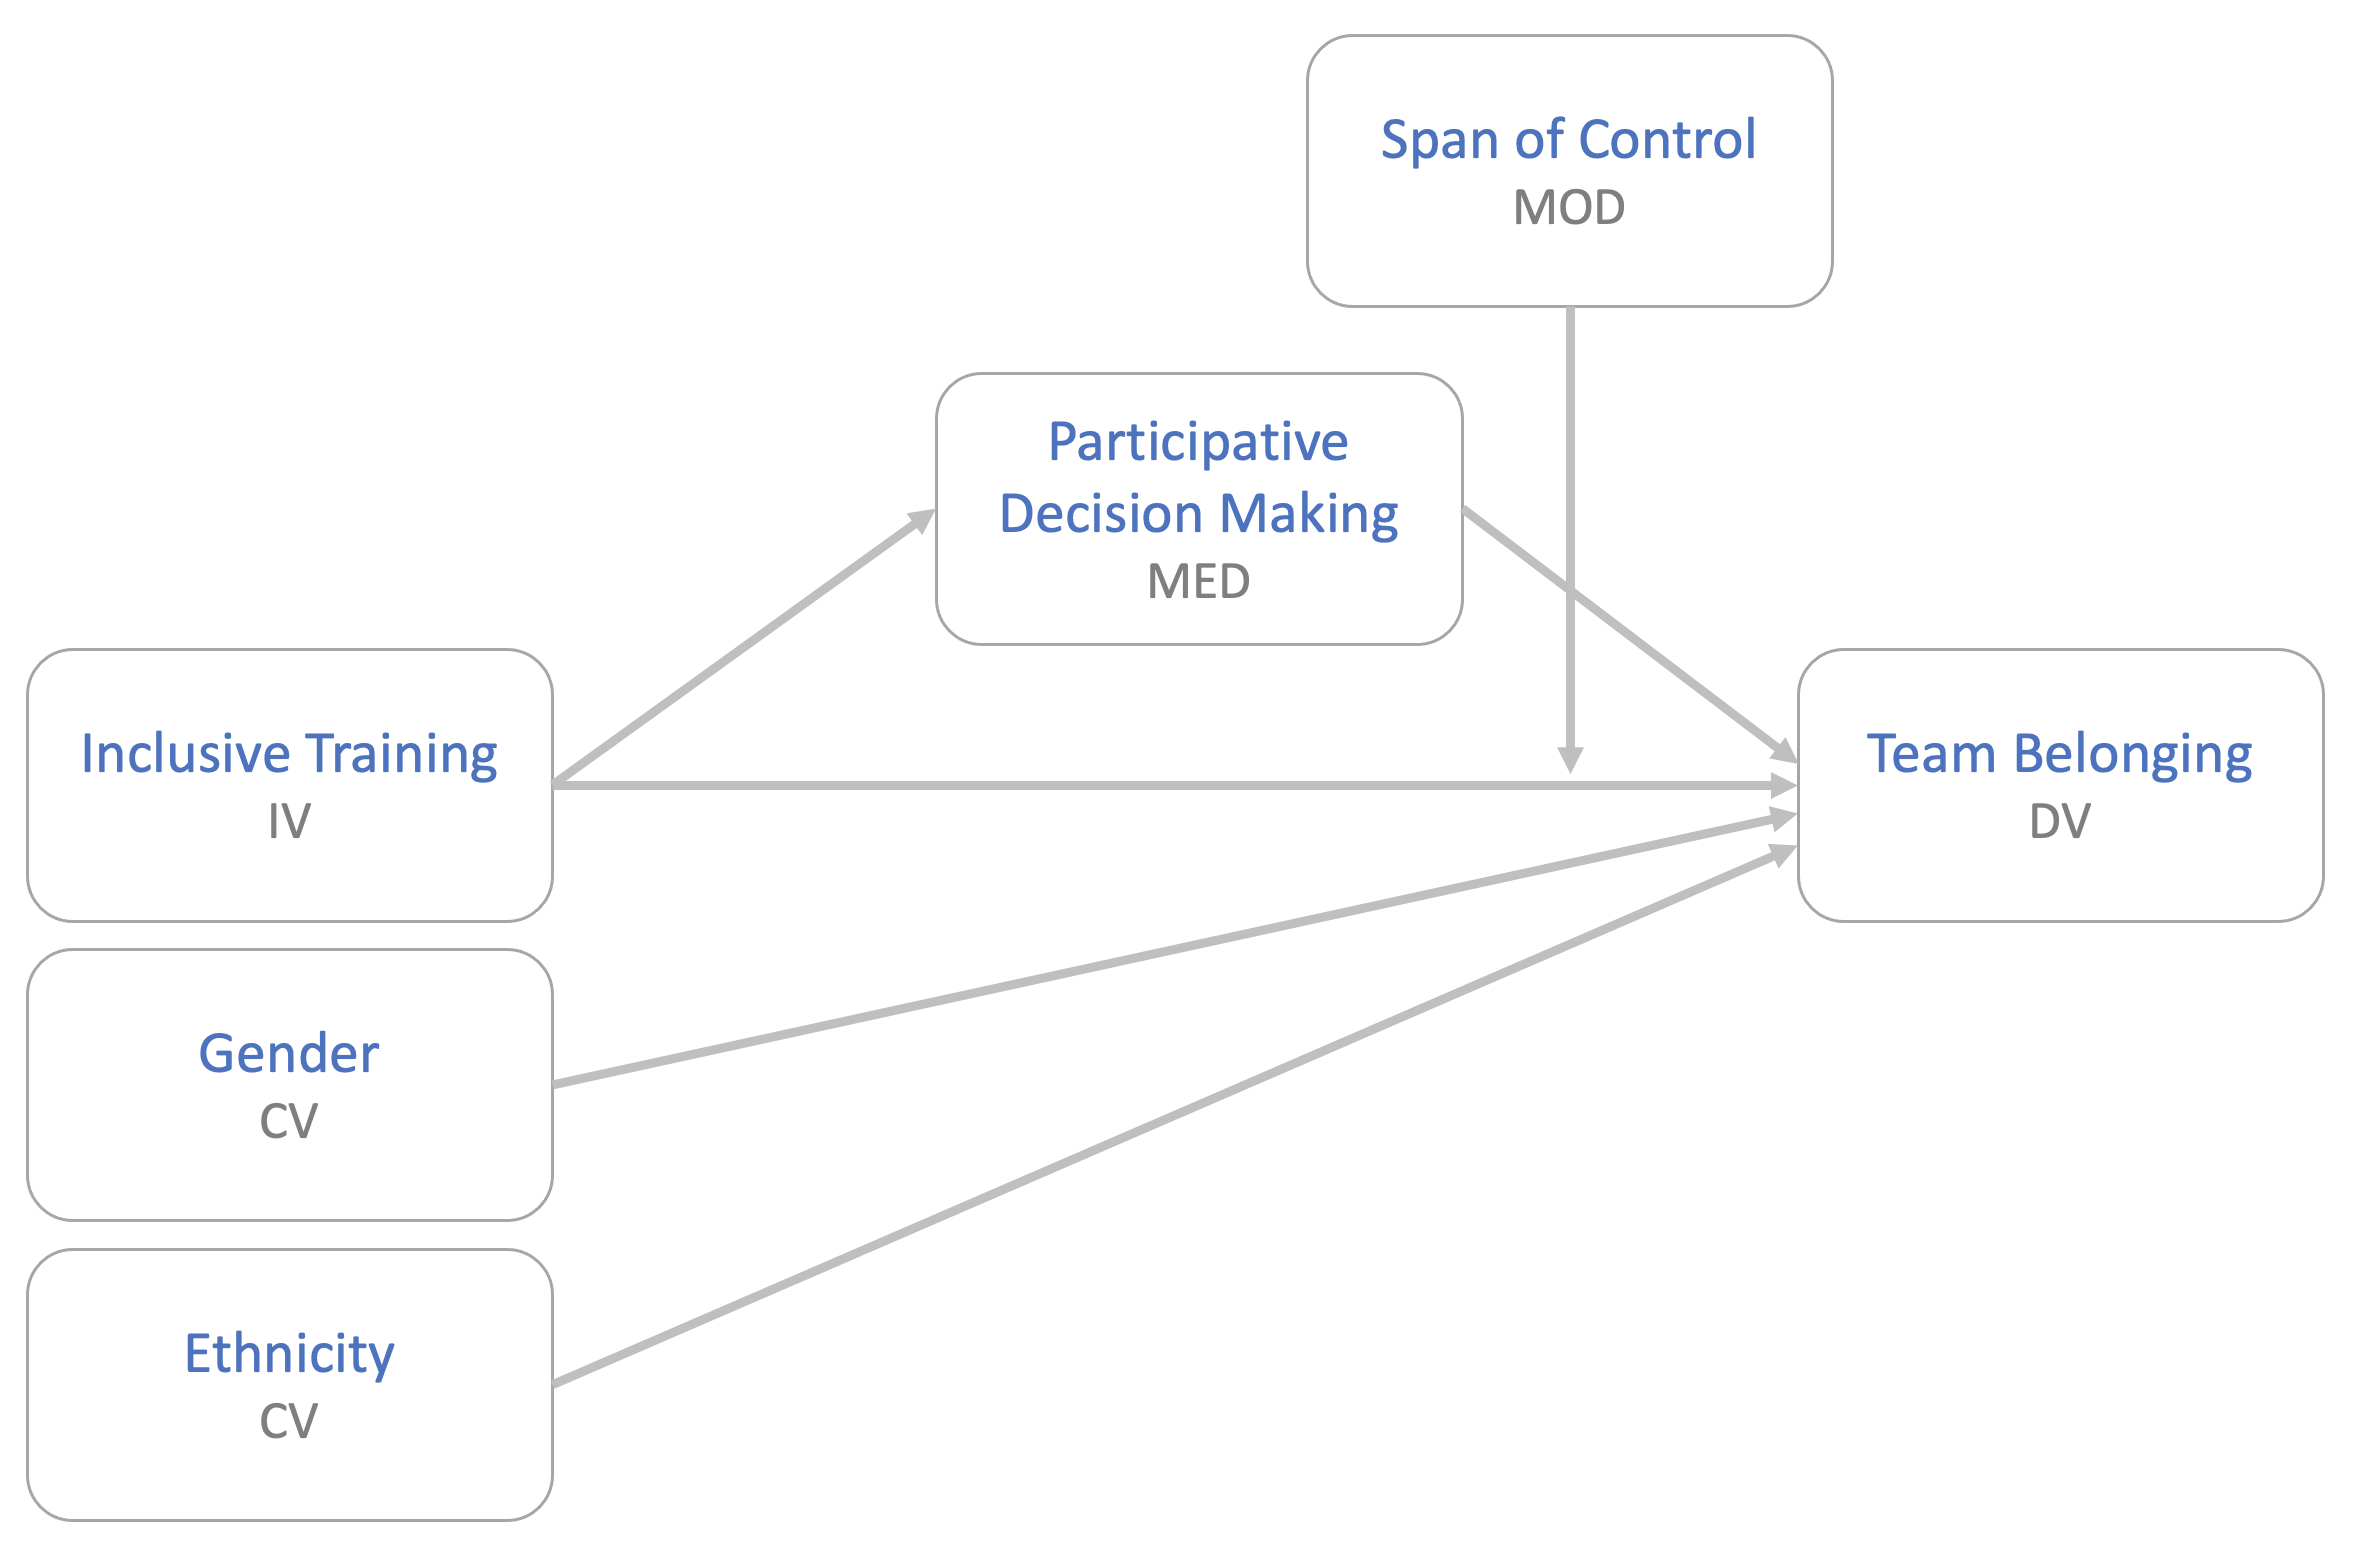
\includegraphics[width=0.75\linewidth]{/Users/craig.starbuck/Library/Mobile Documents/com~apple~CloudDocs/Documents/People Analytics Book/GitHub/peopleanalytics_lifecycle_book/graphics/conceptual_model} 

}

\caption{Conceptual Model of Hypothesized Relationships among Variables}\label{fig:concept-mdl}
\end{figure}

\hypertarget{measurement-scales}{%
\section{Measurement Scales}\label{measurement-scales}}

\textbf{Measurement scales} are used to categorize and quantify variables. There are two major categorizations -- \emph{discrete} and \emph{continuous} -- and these, together with the research hypotheses, help determine appropriate types of analyses to perform.

\hypertarget{discrete-variables}{%
\subsection{Discrete Variables}\label{discrete-variables}}

\textbf{Discrete variables} are also known as \emph{categorical} or \emph{qualitative} variables. Categorical variables have a finite or countable number of values associated with them, and these can be further categorized as either \emph{nominal} or \emph{ordinal}.

\textbf{Nominal}

A \textbf{nominal} variable is one with two or more categories for which there is no intrinsic ordering to the categories. Examples of nominal variables include office locations, departments, and teams. A \textbf{dichotomous variable} is a type of nominal variable which has only two unordered categories. Examples of dichotomous variables include people leader vs.~individual contributor, active vs.~inactive status, and remote worker vs.~non-remote worker.

\textbf{Ordinal}

An \textbf{ordinal} variable is like a nominal variable with one important difference: ordinal variables have \emph{ordered} categories. Examples of ordinal variables include education levels, job levels, and survey variables measured on Likert-type scales.

\hypertarget{continuous-variables}{%
\subsection{Continuous Variables}\label{continuous-variables}}

\textbf{Continuous variables} are also known as \emph{quantitative} variables. Continuous variables can assume any real value in some interval, and these can be further categorized as either \emph{interval} or \emph{ratio} variables.

\textbf{Interval}

Variables measured on an \textbf{interval} scale have a natural order and a quantifiable difference between values but no absolute zero value. Examples include SAT scores, IQ scores, and temperature measured in Fahrenheit or Celsius (but not Kelvin). In these examples, 0 is either not an option (i.e., SAT and IQ) or does not represent the absence of something (e.g., 0 degrees is a temperature, albeit a cold one!).

\textbf{Ratio}

Variables measured on a \textbf{ratio} scale have the same properties as data measured on an interval scale with one important difference: ratio data have an absolute zero value. Examples include compensation, revenue, and sales; a zero in these contexts is possible and would indicate a true absence of something.

\hypertarget{sampling}{%
\section{Sampling}\label{sampling}}

The goal of research is to understand a population based on data from a subset of population members. In practice, it is often not feasible to collect data from every member of a population, so we instead calculate \textbf{sample statistics} to estimate \textbf{population parameters}.

Another important concept is the \textbf{sampling frame}. While the population represents the entire group of interest, the sampling frame represents the subset of the population to which the researcher has access. In an ideal setting, the population and sampling frame are the same, but they are often different in practice. For example, a professor may be interested in understanding student sentiment about a new school policy but only has access to collect data from students in the courses she teaches. In this case, the entire student body is the population but the students she has access to (those in the courses she teaches) represent the sampling frame. The sample is the subset of the sampling frame that ultimately participates in the research (e.g,. those who complete a survey or participate in a focus group).

\hypertarget{sampling-nonsampling-error}{%
\subsection{Sampling \& Nonsampling Error}\label{sampling-nonsampling-error}}

Sampling and nonsampling errors are general categorizations of biases and error in research (Albright \& Winston, 2016).

\hypertarget{sampling-error}{%
\subsubsection{Sampling Error}\label{sampling-error}}

\textbf{Sampling error} is the inevitable result of basing inferences on a random sample rather than the entire population. The two main contributors to sampling error are the size of the sample and variation in the underlying population. The risk of sampling error decreases as the sample size approaches the population size; however, it is usually not feasible to gain information from the entire population, so sampling error is generally a concern.

\textbf{Selection Bias}

\textbf{Selection bias} is the bias introduced by a non-random method of selecting data for analysis, which can systematically skew results in a particular direction. Selection bias may result in observed relationships or differences that are not due to true relationships or differences in the underlying populations, but to the way in which participants or data were selected for the research.

A type of selection bias that is important to consider in people analytics is \textbf{survival bias}. In people analytics, survival bias is the logical error of focusing only on people who made it past some selection process while overlooking those who did not. For example, to gain an accurate understanding of the number of employees who \emph{survive} to each tenure milestone (e.g., 1 year, 2 years, 3 years, etc.), we need to study both active and inactive people to avoid biased results. We may find a significant drop in the percent of active employees who survive from 3 to 4 years, for example, but without information on inactive employees we do not know if this is a function of hiring (i.e., relatively few hired more than 3 years ago) or due to a spike in attrition beyond 3 years of tenure.

The work of a mathematician named Abraham Wald during World War II is a classic example of survival bias. Wald was a member of the Statistical Research Group (SRG) at Columbia University that examined damage to returning aircraft (Wald, 1943). Rather than focusing on the areas with damage, Wald recommended a different way of looking at the data, suggesting that the reason certain parts of planes were not covered in bullet holes was because planes that were shot in these areas did not return. In other words, locations with bullet holes represented locations that could sustain damage and still return home. This insight led to armor being reinforced in areas with no bullet holes.

\begin{figure}

{\centering 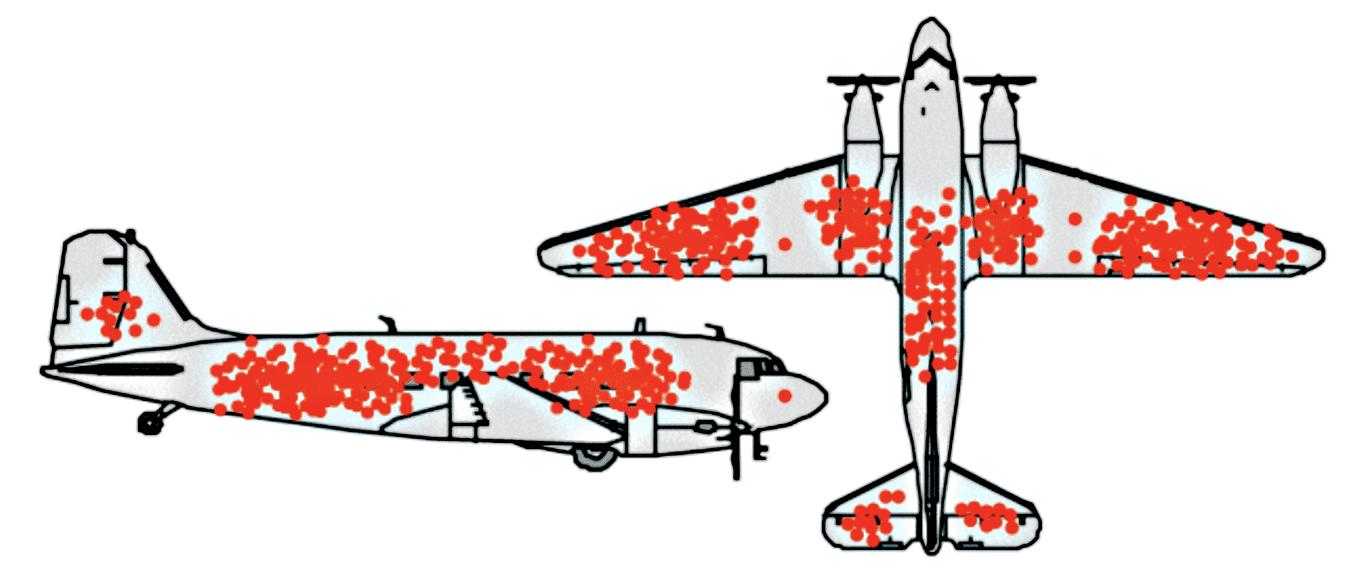
\includegraphics[width=0.75\linewidth]{/Users/craig.starbuck/Library/Mobile Documents/com~apple~CloudDocs/Documents/People Analytics Book/GitHub/peopleanalytics_lifecycle_book/graphics/ww2_plane_damage} 

}

\caption{Hypothetical Data for Damaged Portions of Returning WWII Planes. Image Courtesy of Wikimedia Commons.}\label{fig:ww2-plane-damage}
\end{figure}

Missing data can sometimes be more valuable than the data we have, and it is critical to promote a representative data generative process to prevent biased selection and results.

It is important to understand the centrality of \textbf{randomness} in sampling. Randomization protects against subjective biases, self-validates the data, and is the key ingredient that defines the representative means of extracting information (Kahneman, 2011). Sample data that are not representative of the population of interest can lend to anomalies -- mere coincidences. While non-random data can be leveraged for directionally accurate insights, randomness is required to make inferences about a broader population with a reasonable degree of confidence.

Let's consider an example from Kahneman (2011) in which six babies are born in sequence at a hospital. The gender of these babies is of course random and independent; the gender of one does not influence the gender of another. Consider the three possible sequences of girls (G) and boys (B) below:

\begin{itemize}
\tightlist
\item
  BBBGGG
\item
  GGGGGG
\item
  BGBBGB
\end{itemize}

Are these sequences equally likely? Though it may initially be counter-intuitive, since the events are independent and the outcomes (B and G) are (approximately) equally likely, any possible sequence of births is as likely as any other.

Sample size (colloquially referred to as the \(n\)-count) is also important as this can have a material influence on the representativeness of sample data -- and consequently, the veracity of results and conclusions based on them. As we will explore in Chapter \ref{inf-stats}, as the sample size increases, so too does our confidence that estimates based on sample data reflect population parameters.

To illustrate the effects of sample sizes, let's consider a hypothetical study in which the promotion rate in an organization is found to be lowest in divisions that are primarily software engineers, low diversity, small, and geographically dispersed. Which of these characteristics might offer an explanation? Let's consider that this study also found that the divisions with highest promotion rates have identical characteristics: software engineers, low diversity, small, and geographically dispersed.

Small samples yield extreme results more often than large samples. Small samples neither cause nor prevent outcomes; they merely allow the incidence of the outcome to be much higher (or much lower) than it is in the larger population (Kahneman, 2011).

\textbf{Non-Probability Sampling}

\textbf{Non-probability sampling} can help us gain insight into the \emph{possible}. However, we cannot make inferences based on data collected through non-probability sampling methods since the sample is unlikely to be representative of the population.

\textbf{Convenience (Accidental) Sampling}

\textbf{Convenience sampling} is the most common type of nonprobabilistic sampling. This sampling method involves taking samples that are conveniently located around a specific location (physical or virtual).

For example, if we were to study employee sentiment about new benefit plans by polling employees walking through the lobby of a particular office building one morning, this would represent convenience sampling. Aside from the risk of employees sharing socially desirable responses in such a setting and invalidating the results, a major shortcoming of this approach is that we are only capturing the sentiment of those who happen to walk into one particular building during one limited window of time. This would not capture the voice of employees who are working remotely, working in another office location, on PTO, taking a sick day, attending an offsite conference or meeting, or stuck in traffic and running late.

\textbf{Quota Sampling}

\textbf{Quota sampling} is a nonprobabilistic sampling method in which researchers for a sample that is representative of a larger population. With quota sampling, researchers assign quotas to a group of people to create subgroups of individuals that reflect the characteristics of the population. This is nonprobabilistic since researchers choose the sample rather than randomly selecting it.

For example, if the characteristics of the employee population are known, the researcher polling employees in the office lobby about benefit plans could collect some additional information (e.g., department, job, tenure) to achieve a commensurate proportion of each in the sample. If 30\% of employees in the larger workforce are in the Engineering department, the researcher could assign a quota -- such as 3 in every 10 participants -- to \emph{choose} a sample in which 30\% of employees come from the Engineering department.

\textbf{Purposive (Judgmental) Sampling}

The main goal of \textbf{purposive sampling} is to construct a sample by focusing on characteristics of a population that are of interest to the researcher. Purposive sampling is often used in qualitative or mixed methods research contexts in which a smaller sample is sufficient. Since it is a nonprobabilistic sampling method, purposive sampling is highly prone to researcher bias.

For example, the People Team may be interested in understanding what is top-of-mind for employees in order to design a survey with relevant items. The team may choose people to participate in focus groups to surface qualitative themes -- not for the purpose of generalizing findings but to guide survey item selection efforts.

\textbf{Probability Sampling}

\textbf{Probability sampling} can help us gain insight into the \emph{probable}. The main difference between non-probability and probability sampling is that non-probability sampling does not involve random selection and probability sampling does. Probability sampling is intended to facilitate inferences since data collected through random selection methods is more likely to be representative of the population and protects against over-indexing on participants with similar qualities in the sample.

\textbf{Simple Random Sampling}

\textbf{Simple random sampling} is a method in which each member of the population has the same probability of being selected for a sample. An example of simple random sampling is randomly selecting a specified number or percent of employees from the workforce to participate in a survey without regard for tenure, department, level, or other characteristics.

We can use the sample() function in R to randomly select from a vector of elements:

\begin{Shaded}
\begin{Highlighting}[]
\CommentTok{\# Load library for data wrangling}
\FunctionTok{library}\NormalTok{(dplyr)}

\CommentTok{\# Read employee data}
\NormalTok{employees }\OtherTok{\textless{}{-}} \FunctionTok{read.csv}\NormalTok{(}\StringTok{"/Users/craig.starbuck/Library/Mobile Documents/com\textasciitilde{}apple\textasciitilde{}CloudDocs/Documents/People Analytics Book/GitHub/peopleanalytics\_lifecycle\_book/data/employees.csv"}\NormalTok{)}

\CommentTok{\# Set seed for reproducible results}
\FunctionTok{set.seed}\NormalTok{(}\DecValTok{1234}\NormalTok{)}

\CommentTok{\# Sample 10 employees randomly}
\NormalTok{n }\OtherTok{=} \DecValTok{10}
\FunctionTok{sample}\NormalTok{(employees}\SpecialCharTok{$}\NormalTok{employee\_id, n, }\AttributeTok{replace =}\NormalTok{ F)}
\end{Highlighting}
\end{Shaded}

\begin{verbatim}
##  [1] 2308 2018 2125 2004 1623 1905 1645 1934 1400 1900
\end{verbatim}

The \texttt{replace\ =\ F} argument in the sample() function indicates that we want to sample \emph{without} replacement (i.e., we do not want an employee to be selected twice in the sample). For example, if we draw multiple names from a hat without replacement, we will not put names back into the hat once they are drawn; each has a chance of being selected only once.

While sampling \emph{with} replacement would not make sense for applications such as pulse survey participation, as we would not want a given employee to take a survey multiple times, \texttt{replace\ =\ T} can be applied if the application requires it (e.g., a lottery in which employees can win more than once).

\textbf{Stratified Random Sampling}

\textbf{Stratified random sampling} is a sampling method in which the population is first divided into \emph{strata}. Then, a simple random sample is taken from each \emph{stratum} -- a homogeneous subset of the population with similar characteristics with regard to the variable of interest. The combined results constitute the sample.

To ensure samples do not comprise a larger proportion of employees from a particular department, education level, tenure band, generational cohort, or other variable deemed useful in explaining differences in response scores, researchers can randomly select members for each stratum based on the proportion in the respective stratum in the larger population. For example, if 30\% of all employees are in the Engineering department, the researcher could \emph{randomly} select a calculated number of employees from the Engineering department such that 30\% of employees in the sample come from this department.

Let's demonstrate stratified random sampling in R by sampling \(\frac{1}{2}\) of employees within each department. First, we can review counts of employees for each department using the group\_by() and summarise() functions from the \texttt{dplyr} library. Note that \texttt{dplyr} functions are chained together using a \texttt{\%\textgreater{}\%} symbol:

\begin{Shaded}
\begin{Highlighting}[]
\CommentTok{\# Return employee counts by department}
\NormalTok{employees }\SpecialCharTok{\%\textgreater{}\%}
\FunctionTok{group\_by}\NormalTok{(dept) }\SpecialCharTok{\%\textgreater{}\%}
\FunctionTok{summarise}\NormalTok{(}\AttributeTok{n =} \FunctionTok{n}\NormalTok{())}
\end{Highlighting}
\end{Shaded}

\begin{verbatim}
## # A tibble: 3 x 2
##   dept                       n
##   <chr>                  <int>
## 1 Human Resources           63
## 2 Research & Development   961
## 3 Sales                    446
\end{verbatim}

Next, we will randomly select \(\frac{1}{2}\) of employees within each department using the group\_by() and sample\_frac() functions from the \texttt{dplyr} library. We will store the selected employees' records in a data frame and then query it to validate that the counts are roughly \(\frac{1}{2}\) the total count observed for each department.

\begin{Shaded}
\begin{Highlighting}[]
\CommentTok{\# Obtain and store stratified random sample}
\NormalTok{strat\_sample }\OtherTok{\textless{}{-}}\NormalTok{ employees }\SpecialCharTok{\%\textgreater{}\%}
                \FunctionTok{group\_by}\NormalTok{(dept) }\SpecialCharTok{\%\textgreater{}\%}
                \FunctionTok{sample\_frac}\NormalTok{(}\AttributeTok{size =}\NormalTok{ .}\DecValTok{5}\NormalTok{)}

\CommentTok{\# Return sample counts by department}
\NormalTok{strat\_sample }\SpecialCharTok{\%\textgreater{}\%}
\FunctionTok{group\_by}\NormalTok{(dept) }\SpecialCharTok{\%\textgreater{}\%}
\FunctionTok{summarise}\NormalTok{(}\AttributeTok{n =} \FunctionTok{n}\NormalTok{())}
\end{Highlighting}
\end{Shaded}

\begin{verbatim}
## # A tibble: 3 x 2
##   dept                       n
##   <chr>                  <int>
## 1 Human Resources           32
## 2 Research & Development   480
## 3 Sales                    223
\end{verbatim}

\textbf{Cluster Sampling}

\textbf{Cluster sampling} is a sampling method often used in market research in which the population is first divided into clusters. Then, a simple random sample of clusters is taken. All the members of the selected clusters together constitute the sample. Unlike stratified random sampling, it is the clusters that are selected at random -- not the individuals. It is hoped that each cluster by itself is representative of the population (i.e., each cluster is heterogeneous).

For example, employees could be partitioned into clusters based only on their geographic region. Since there is not further partitioning on other variables, each cluster is expected to be heterogeneous on the basis of variables other than geographic region -- that is, unless geography is related to other variables (e.g., call center employees are all located in a company's Pacific Northwest region). By selecting a random set of clusters, the combination of employees across the selected clusters is expected to be representative of the population.

Let's demonstrate how to implement cluster sampling in R:

\begin{Shaded}
\begin{Highlighting}[]
\CommentTok{\# Randomly assign each employee to 1 of 10 clusters (groups)}
\NormalTok{employees}\SpecialCharTok{$}\NormalTok{cluster }\OtherTok{\textless{}{-}} \FunctionTok{sample}\NormalTok{(}\DecValTok{1}\SpecialCharTok{:}\DecValTok{10}\NormalTok{, }\AttributeTok{size =} \FunctionTok{nrow}\NormalTok{(employees), }\AttributeTok{replace =}\NormalTok{ T)}

\CommentTok{\# Randomly select 5 clusters}
\NormalTok{clusters }\OtherTok{\textless{}{-}} \FunctionTok{sample}\NormalTok{(}\FunctionTok{unique}\NormalTok{(employees}\SpecialCharTok{$}\NormalTok{cluster), }\AttributeTok{size =} \DecValTok{5}\NormalTok{, }\AttributeTok{replace =}\NormalTok{ F)}

\CommentTok{\# Store cluster sample}
\NormalTok{clust\_sample }\OtherTok{\textless{}{-}}\NormalTok{ employees }\SpecialCharTok{\%\textgreater{}\%}
                \FunctionTok{filter}\NormalTok{(cluster }\SpecialCharTok{\%in\%}\NormalTok{ clusters)}

\CommentTok{\# Display dimensions of the cluster sample object}
\FunctionTok{dim}\NormalTok{(clust\_sample)}
\end{Highlighting}
\end{Shaded}

\begin{verbatim}
## [1] 748  37
\end{verbatim}

\textbf{Systematic Sampling}

\textbf{Systematic sampling} involves selecting sample members from a population according to a random starting point and a fixed, periodic interval known as a sampling interval. The sampling interval is computed by taking the population size and dividing it by the desired sample size. The resulting number is the interval at which population members are selected for the sample.

For example, if there are 10,000 employees and our desired sample size is 500, the sampling interval is 20. Therefore, we would select every 20th employee for our sample. It is important that the sequence does not represent a standardized pattern that would bias the data; this process needs to be random. For example, if the employee id generated by the HRIS increases with time, we would expect employees with longer tenure to have lower employee ids while new joiners would have higher employee ids. Ordering employees by employee id prior to selection could bias the sample on the basis of variables related to tenure (e.g., aggressive periods of Engineering hiring).

Let's walk through the step-by-step process for implementing the systematic sampling procedure in R:

\begin{Shaded}
\begin{Highlighting}[]
\CommentTok{\# Specify desired sample size}
\NormalTok{n }\OtherTok{=} \DecValTok{100}

\CommentTok{\# Determine population size}
\NormalTok{N }\OtherTok{=} \FunctionTok{nrow}\NormalTok{(employees)}

\CommentTok{\# Compute sampling interval, rounding up to nearest whole number via the ceiling() function}
\NormalTok{si }\OtherTok{=} \FunctionTok{ceiling}\NormalTok{(N}\SpecialCharTok{/}\NormalTok{n)}

\CommentTok{\# Randomly select value between 1 and the sampling interval for starting value}
\NormalTok{strt }\OtherTok{=} \FunctionTok{sample}\NormalTok{(}\DecValTok{1}\SpecialCharTok{:}\NormalTok{si, }\DecValTok{1}\NormalTok{)}

\CommentTok{\# Increment starting value by the sampling interval until the desired sample size is achieved, and hydrate index vector with the selected indices}
\NormalTok{index }\OtherTok{=} \FunctionTok{seq}\NormalTok{(strt, strt }\SpecialCharTok{+}\NormalTok{ si }\SpecialCharTok{*}\NormalTok{ (n }\SpecialCharTok{{-}} \DecValTok{1}\NormalTok{), si)}

\CommentTok{\# Store systematic sample}
\NormalTok{syst\_sample }\OtherTok{\textless{}{-}}\NormalTok{ employees[index, ]}
\end{Highlighting}
\end{Shaded}

\hypertarget{nonsampling-error}{%
\subsubsection{Nonsampling Error}\label{nonsampling-error}}

There are many types of \textbf{nonsampling error} that can invalidate results beyond the sampling procedure, and we will focus on several that are particularly germane to people analytics: \emph{nonresponse bias}, \emph{nontruthful responses}, \emph{measurement error}, and \emph{voluntary response bias}.

\textbf{Nonresponse Bias}

Surveys are a staple in the set of data sources germane to people analytics. While survey data provide unique attitudinal and perceptive signals that can be highly predictive of future behavior and events, surveys tend to be far more susceptible to nonsampling error than other data sources.

As discussed in the context of sampling error, we usually do not have access to information on entire populations of interest, so we must consider the possibility that those for whom we are missing data may have common qualities, perceptions, or opinions that differ from those for whom we do have data. This is known as \textbf{nonresponse bias}. For example, if we administer an employee experience survey to the entire organization and receive a 60\% response rate, the reality is that we do not know how the 40\% of nonrespondents would have responded. It is possible that nonrespondents represent highly disengaged employees, in which case their responses may have materially influenced results and conclusions in an unfavorable direction. It is also possible that nonrespondents did not participate because they were busy, away on vacation, cynical to the confidentiality language in the communications, or any number of other reasons which may or may not have resulted in significantly different feedback from that of respondents.

As an aside, nonrespondents can actually function as an important variable in analyses. In some contexts, nonrespondents may be at greater risk of voluntary attrition than those who respond unfavorably on a stay intentions survey item such as, ``I plan to be working here in one year.'' Evaluating response rate distributions across departments, divisions, roles, and other dimensions may be an insightful endeavor.

Nonresponse bias is not limited to surveys. For example, self-reported demographics such as gender and ethnicity may not be disclosed by all employees in the HR information system (HRIS). This can bias segmentations based on these categorical dimensions. While there are strategies to address this, such as visual ID or applying models trained to infer missing values (which may be necessary to fulfill EEOC reporting requirements), there may still be error in the imputed values.

\textbf{Nontruthful Responses}

While high response rates may reduce nonresponse bias, this isn't always something to celebrate. Organizations that incentivize participation in surveys often do so at the risk of people responding in socially desirable ways and providing \textbf{nontruthful responses} to achieve some defined target. For example, if an employee has an unhealthy relationship with his manager but does not trust that managers will not have access to individual-level responses, the employee may decide to indicate on the survey that everything is highly favorable to help the team win the month of casual days leadership promised. This can of course skew and invalidate results.

While survey participation should be strongly encouraged since higher response rates can mitigate the risk of certain types of bias and increase confidence that the survey is representative of the collective organization's sentiments, incentivizing participation can be dangerous.

\textbf{Measurement Error}

The measurement method can affect observed data either by changing the underlying construct of interest, or by distorting the measurement process without impacting the construct itself (Spector, 2006).

\textbf{Common method variance (CMV)}, also known as \textbf{monomethod bias}, relates to a widely held belief that relationships between variables measured using the same method are inflated. The idea that the measurement method itself introduces a degree of variance in measures has been cited in organizational papers for decades, and it is raised almost exclusively when cross-sectional, self-reported surveys are utilized. Though controversial, there is generally a consensus that where it is possible to do so, it is preferrable to leverage multiple measurement methods.

My doctoral dissertation research explored how implicit voice theories, which are deep-seated beliefs about the risks involved in speaking up to those higher in the organizational hierarchy (e.g., negative career consequences), influenced the extent to which individual contributors actually speak up in prosocial ways to their leaders (Starbuck, 2016). Since the individual contributors are best placed to provide information on the implicit beliefs they maintain, data for the IV were collected using cross-sectional self-reports. At the same time, I surveyed their immediate supervisors and asked them to rate each of their direct reports using a leader-directed voice scale; these supervisor-reports of leader-directed voice were used as the DV in this study. To investigate CMV, which was a tangential interest to the primary research objective, I also included the leader-directed voice scale (using self-reported language) on the survey administered to individual contributors.

For the 1,032 employees from whom I collected data in an investment firm context (individual contributors: \(n\) = 696; supervisors: \(n\) = 336), I was surprised to find only a weak correlation between self-reported voice and supervisor-reported voice (\(r\) = .26, \(p\) \textless{} .01). On average, self-reported voice was higher with less variation (\(\bar{x}\) = 5.91, \(s\) = 1.15) relative to supervisor-reported voice (\(\bar{x}\) = 5.69, \(s\) = 1.34). Interestingly, there was support for almost none of the hypothesized relationships when supervisor-reported voice was positioned as the DV, though most were supported when self-reported voice was substituted as the DV in post-hoc analyses. Given the prevalence of monomethod self-reports in the social sciences, the influence of CMV is an important consideration.

\textbf{Measurement error} relates to errors stemming from confusing questions, survey fatigue, and low-quality scales used to measure multidimensional psychological constructs. The field of \textbf{psychometrics} is a vast scientific discipline concerned with the development of assessment tools, measurement instruments, and formalized models to understand latent psychological constructs such as engagement, belonging, purpose, and wellbeing using observable indicators.

The reduction of measurement error is a principal concern to psychometricians. For a deeper treatment of the survey scale development process, see DeVellis (2012). While an exhaustive treatment of psychometrics is beyond the scope of this book, \emph{reliability} and \emph{validity} are two broad sets of methods designed to increase the robustness of psychological instrumentation which will be reviewed in this section. Even slight adjustments to validated instrumentation -- such as changing the number of scale anchors (e.g., increasing from a 5-point to 7-point Likert scale), tweaking item language, or modifying which items are included in a composite scale -- generally warrant reliability and validity analyses.

Figure \ref{fig:reli-vali} illustrates differences between reliability and validity.

\begin{figure}

{\centering 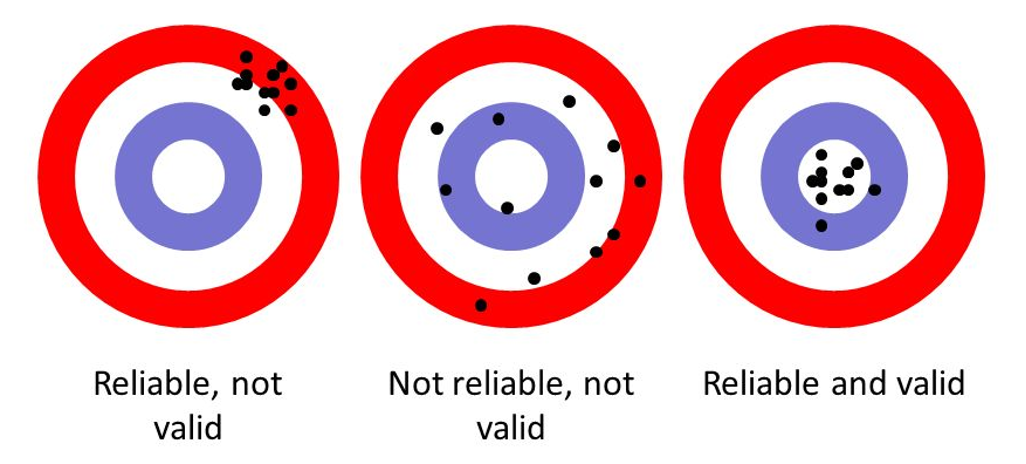
\includegraphics[width=0.75\linewidth]{/Users/craig.starbuck/Library/Mobile Documents/com~apple~CloudDocs/Documents/People Analytics Book/GitHub/peopleanalytics_lifecycle_book/graphics/reliability_validity} 

}

\caption{Reliability and Validity}\label{fig:reli-vali}
\end{figure}

A weight scale may be a helpful example for understanding differences between these concepts. A weight scale is designed to provide an accurate measurement of one's weight, and we expect measurements to be consistently accurate over time. If a 150 lb. person steps onto a weight scale and receives a reading of 180 lbs., the scale is not valid as the person actually weighs 30 lbs. less than the reading. If the person steps onto the scale a second time moments later and receives a reading of 200 pounds, the scale is not reliable either (inconsistent measurements). As researchers, it is critical to measure what we intend to measure (validity) and do it with consistency (reliability). Survey items with poor psychometric properties can lend to invalid conclusions due to measurement error.

\textbf{Reliability} describes the quality of measurement (i.e., the consistency or repeatability of measures). Types of reliability include:

\begin{itemize}
\tightlist
\item
  \textbf{Inter-Rater or Inter-Observer Reliability}: the degree to which different raters/observers give consistent estimates of the same phenomenon.
\item
  \textbf{Test-Retest Reliability}: the consistency of a measure from one time to another.
\item
  \textbf{Parallel-Forms Reliability}: the consistency of the results of two tests constructed in the same way from the same content domain.
\item
  \textbf{Internal Consistency Reliability}: the consistency of results across items within a test.
\end{itemize}

\textbf{Validity} describes how well a concept was translated into a functioning and operating reality (operationalization). There are four main types of validity: (a) \emph{face validity}, (b) \emph{content validity}, (c) \emph{construct validity}, and (d) \emph{criterion-related validity}:

\textbf{Face validity}

\textbf{Face validity} is an assessment of how valid a measure appears on the surface. In other words, face validity represents whether the measurement approach ``on its face'' is a good translation of the construct. This is the least scientific method of validity and should never be accepted on its own merits.

\textbf{Content Validity}

\textbf{Content validity} is a somewhat subjective assessment of whether a measure covers the full content domain. Content validity relies on people's perceptions to measure constructs that would otherwise be difficult to measure.

For example, a panel of experts may gather to discuss the various dimensions of a theoretical construct. The psychometrician may then use this information to develop survey items that tap these dimensions to achieve a comprehensive measure of the construct.

\textbf{Construct Validity}

In social science, constructs are often measured using a collection of related indicators that together, tap the various dimensions of the theoretical idea. Constructs may manifest in a set of behaviors, which provide evidence for their existence. \textbf{Construct validity} represents the degree to which a collection of indicators and behaviors -- the \textbf{operationalization} of the concept -- truly represents theoretical constructs.

Psychological safety, a belief that a context is safe for interpersonal risk-taking (Edmondson, 1999), has no direct measure. However, there are indicators and behaviors that are helpful in understanding the extent to which an environment is psychologically safe. We may ask employees whether they are able to bring up problems to decision makers or whether it is safe to take risks on their team. Based on the theoretical conception of psychological safety, these would be helpful (though not exhaustive) indicators of the construct in an organizational setting.

There are two types of construct validity:

\begin{itemize}
\tightlist
\item
  \textbf{Convergent validity}: the degree to which the operationalization is similar to (converges on) other operationalizations to which it theoretically should be similar.
\item
  \textbf{Discriminant validity}: the degree to which the operationalization is not similar to (diverges from) other operationalizations to which it theoretically should not be similar.
\end{itemize}

A \textbf{nomological network} is central to providing evidence for a measure's construct validity. The nomological network is an idea developed by Cronbach and Meehl (1955) to represent the constructs of interest, their observable manifestations, as well as the interrelationships among them. The term ``nomological'' is derived from the Greek word meaning ``lawful''; therefore, the nomological network aims to make clear what a construct means so that laws (nomologicals) can be applied. Simply put, the nomological network attempts to link the conceptual and theoretical realm to the observable one to provide a practical methodology for assessing a measure's construct validity.

If psychological safety theory suggests the construct should be positively related to leader openness and negatively associated with employee withholding (silence), we can use validated measures of openness and withholding to test for these theoretical relationships with psychological safety and substantiate construct validity.

\textbf{Criterion-Related Validity}

\textbf{Criterion-related validity}, sometimes referred to as \emph{instrumental validity}, describes how well scores from one measure are adequate estimates of performance on an outcome measure (or \emph{criterion}).

There are two types of criterion-related validity:

\begin{itemize}
\tightlist
\item
  \textbf{Predictive validity}: the operationalization's ability to predict something it should theoretically be able to predict.
\item
  \textbf{Concurrent validity}: the operationalization's ability to distinguish between groups that it should theoretically be able to distinguish between.
\end{itemize}

If psychological safety should positively influence employee voice, there would be support for predictive validity if we find that employees who report more favorable perceptions of psychological safety are more willing to speak up. If we administer a new scale to measure psychological safety and \emph{at the same time} (concurrently) administer an existing, validated measure of the same construct, highly correlated results would lend support for the new measure's concurrent validity.

\hypertarget{review-questions-2}{%
\section{Review Questions}\label{review-questions-2}}

\begin{enumerate}
\def\labelenumi{\arabic{enumi}.}
\item
  What are the differences between parameters and statistics?
\item
  How does a sampling frame differ from a sample?
\item
  How does cluster sampling differ from stratified random sampling?
\item
  What is the primary benefit of probabilistic sampling methods over non-probabilistic sampling?
\item
  Is nonresponse bias only applicable in the context of surveys?
\item
  What type of variable influences the strength of the effect one variable has on another?
\item
  100 randomly selected employees in the Marketing department of an organization participated in a survey on career pathing for marketing professionals. What is the sample and what is the population in this case?
\item
  How does the meaning of zero differ between interval and ratio-scaled variables?
\item
  Can discrete variables have more than 2 values?
\item
  What are some examples of nonprobabilistic sampling methods?
\end{enumerate}

\hypertarget{research}{%
\chapter{Research Fundamentals}\label{research}}

The importance of appropriate research methods and designs cannot be overstated. Just as probability sampling methods help us achieve data that are representative of the population, research methods and designs help us achieve an accurate understanding of various phenomena and ensure conclusions are justified.

\hypertarget{research-questions}{%
\section{Research Questions}\label{research-questions}}

\textbf{Research questions} are fundamental to all research projects. Research questions help focus the study, determine the appropriate methodology, and guide each stage of inquiry, analysis, and reporting. Some examples of research questions germane to people analytics include:

\begin{itemize}
\tightlist
\item
  \(Q_1\): Why has there been an increase in attrition over the past quarter?
\item
  \(Q_2\): How equitable are promotion nominations across the organization?
\item
  \(Q_3\): Are there meaningful differences in the favorability of experiences for remote vs.~non-remote employees?
\item
  \(Q_4\): Do new joiners have the training and resources they need to be successful?
\item
  \(Q_5\): What portion of team performance is attributable to leadership effectiveness?
\end{itemize}

\hypertarget{research-hypotheses}{%
\section{Research Hypotheses}\label{research-hypotheses}}

\textbf{Research hypotheses} are testable statements about the expected outcome of a research project or experiment.

\begin{itemize}
\tightlist
\item
  \(H_1\): Manager satisfaction is a significant predictor of voluntary attrition.
\item
  \(H_2\): Promotion nomination rates are not significantly different by gender and ethnicity.
\item
  \(H_3\): Employee experience favorability is not significantly different between remote and non-remote workers.
\item
  \(H_4\): New hire training perceptions are positively associated with onboarding experience favorability.
\item
  \(H_5\): Leadership effectiveness perceptions explain significant variation in team performance.
\end{itemize}

\hypertarget{internal-vs.-external-validity}{%
\section{Internal vs.~External Validity}\label{internal-vs.-external-validity}}

\textbf{Internal validity} refers to the extent to which confounding variables are controlled. In other words, internal validity reflects the \emph{robustness} of the study.

For example, if a study finds a significant relationship between work location and attrition but considers no other factors or explanations, this would \emph{not} be a robust study. Work location may emerge significant because certain roles for which attrition is higher are more concentrated in one or more geographies. It could also be the case that the company has made acquisitions in new geographies, and the acquired employees have significantly different experiences (and attrition rates) relative to non-acquired employees.

\textbf{Confounding variables} are critically important in the context of internal validity. A confounding variable is an extraneous variable whose presence impacts the variables being studied such that results do not reflect the actual relationships. Studies with weak internal validity often result in spurious associations that \emph{confound} the true relationship between two variables, leading to invalid conclusions and recommendations.

\textbf{External validity} refers to the extent to which study conclusions will hold in other contexts (for other people, in other places, at other times). \emph{Randomization} is fundamental to our ability to generalize and apply findings to other groups or contexts.

If we survey employees to understand sentiments about recent changes in business strategy but exclude groups for which there may be different impacts or perceptions, conclusions about the collective sentiment would be suspect at best.

\hypertarget{research-methods}{%
\section{Research Methods}\label{research-methods}}

There are three major categories of research methods: (1) \emph{quantitative}, (2) \emph{qualitative}, and (3) \emph{mixed methods}.

\begin{enumerate}
\def\labelenumi{\arabic{enumi}.}
\tightlist
\item
  \textbf{Quantitative}

  \begin{itemize}
  \tightlist
  \item
    Addresses ``what'' questions
  \item
    Utilizes numerical data (e.g., surveys, systems)
  \item
    Primarily deductive
  \item
    Used to test hypotheses
  \item
    Involves statistical analyses
  \item
    More objective
  \item
    More generalizable
  \end{itemize}
\item
  \textbf{Qualitative}

  \begin{itemize}
  \tightlist
  \item
    Addresses ``how'' and ``why'' questions
  \item
    Utilizes text data (e.g., focus groups, interviews, open-ended feedback)
  \item
    Primarily inductive
  \item
    Used to formulate theory or hypotheses
  \item
    Involves organizing data into categories or themes
  \item
    More subjective
  \item
    Less generalizable
  \end{itemize}
\item
  \textbf{Mixed Methods}

  \begin{itemize}
  \tightlist
  \item
    Integrates the strengths of both quantitative and qualitative methods within a single study, often leading with qualitative approaches to build theory and hypotheses followed by quantitative methods to test hypotheses
  \end{itemize}
\end{enumerate}

\hypertarget{research-designs}{%
\section{Research Designs}\label{research-designs}}

In addition to determining whether a quantitative, qualitative, or mixed methods study is most appropriate, researchers also need to decide on the type of study within each of these three. \textbf{Research designs} are the types of inquiry within quantitative, qualitative, and mixed methods approaches that issue specific direction for the research procedures (Creswell, 2018). There are multiple taxonomies for research designs, and we will simplify to the most common types.

Within the quantitative category, there are three types of designs: (a) \emph{experimental}, (b) \emph{quasi-experimental}, and (c) \emph{correlational}. As shown in Figure \ref{fig:res-designs}, it is important to understand the centrality of randomization in this decision.

\begin{figure}

{\centering 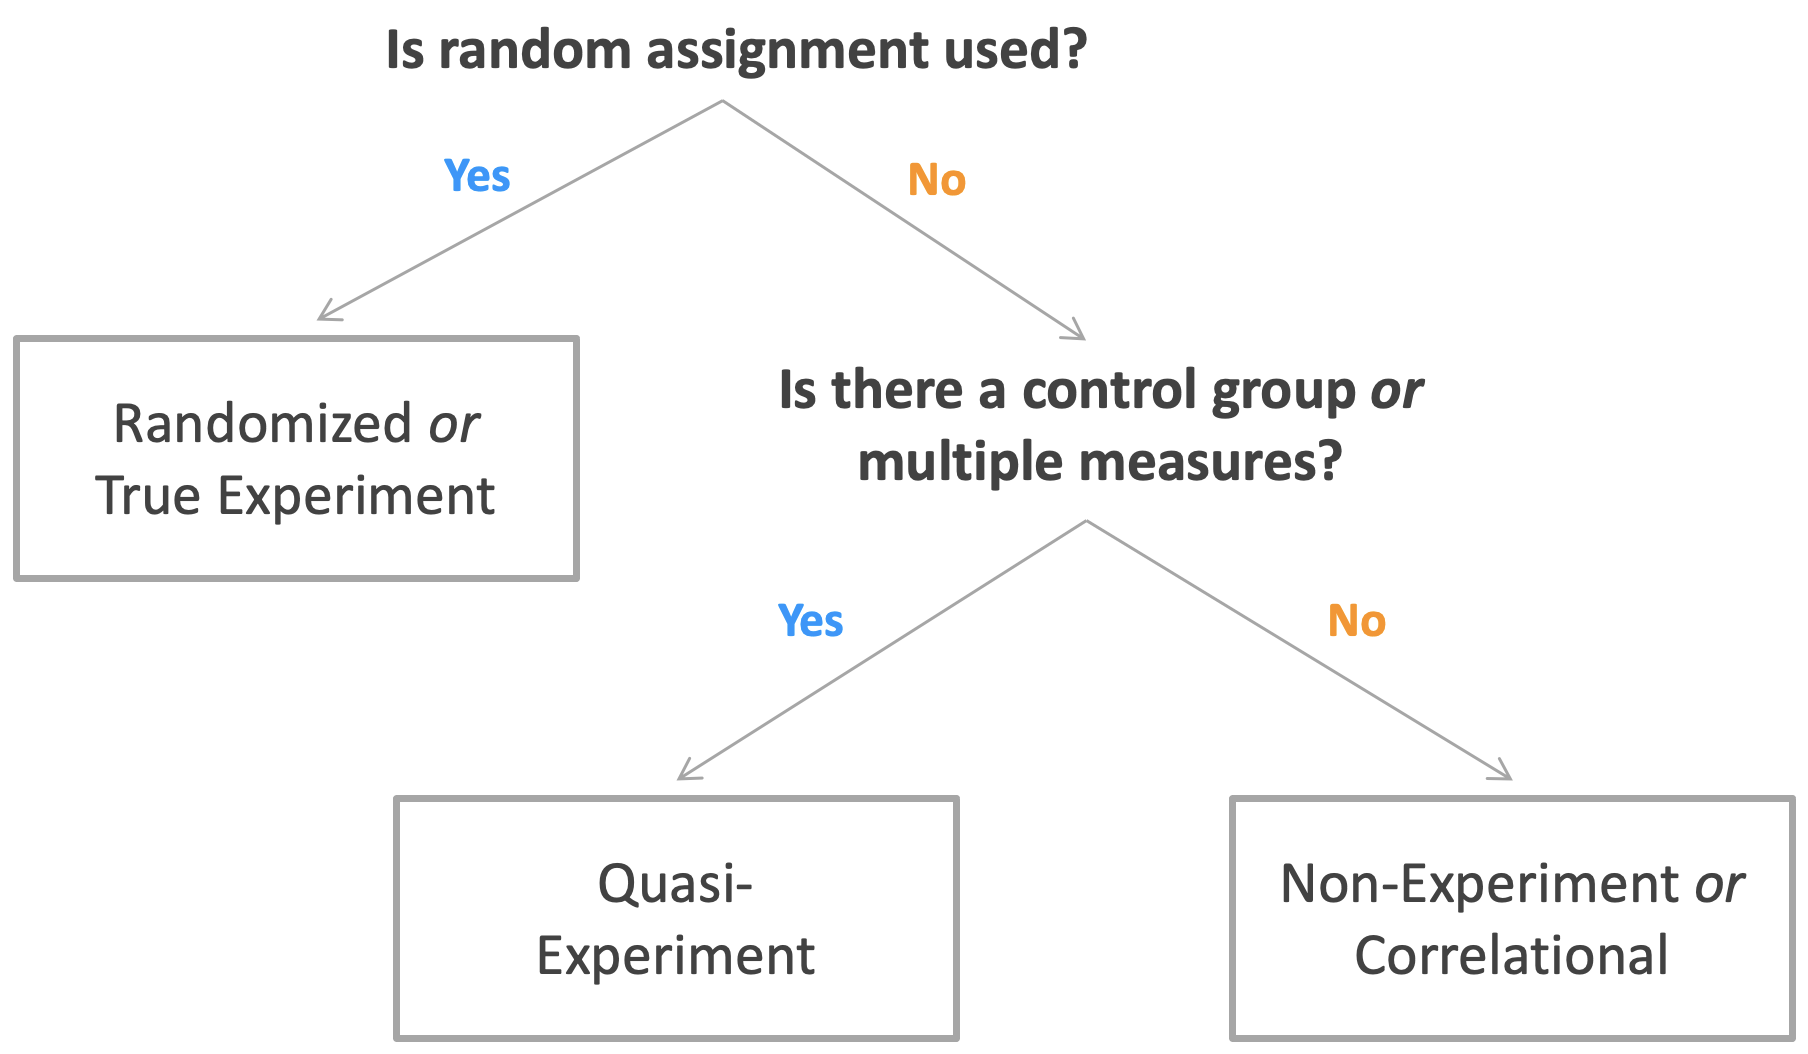
\includegraphics[width=0.75\linewidth]{/Users/craig.starbuck/Library/Mobile Documents/com~apple~CloudDocs/Documents/People Analytics Book/GitHub/peopleanalytics_lifecycle_book/graphics/research_designs} 

}

\caption{Quantitative Research Designs}\label{fig:res-designs}
\end{figure}

\textbf{Experimental Research}

\textbf{Experimental research} is concerned with casual (internal) validity. Randomized experimental designs provide the most rigor with regard to causal validity. However, in social science research contexts, true experiments often are not possible due to ethical considerations.

For example, if we were interested in understanding the causal effect leadership quality has on employee engagement, based on a hypothesis that poor leadership decreases employee engagement, we would need to randomly assign employees to one of two groups that are identical on the basis of all variables that could theoretically explain why employees vary in their levels of engagement. Then, we would need to manipulate the variable of interest (leadership quality) to evaluate if the group of employees subjected to poor leadership (treatment group) reports significantly different levels of engagement relative to the group of employees for whom leadership quality has not been manipulated (control group). In a practical setting, it would of course be unethical to purposefully subject employees to poor leadership with the expectation of reducing engagement -- and consequently, retention, productivity, and impact to the organization.

Clinical trials are a common setting for true experiments, as isolating the effects of an experimental drug can be a matter of life or death. In a randomized clinical trial, patients are randomly assigned to an experimental group (patients who receive the drug) or control group (patients who receive a placebo). To protect against placebo effects biasing the results, patients do not know if they receive the experimental treatment or the placebo. Done correctly, these experiments have the highest level of internal validity.

Another example of an experimental design is \textbf{A/B testing}. A/B testing is often performed in the context of website optimization, in which two or more versions of the site are shown to customers to identify which version impacts key success metrics more positively. In a people analytics context, we may create two versions of a dashboard and \emph{randomly} assign the permissioned users to each. We could then assess whether utilization rates, average usage time, repeat usage, among other success measures are significantly different between the two groups of users to inform which design is most effective.

In experimental research, it is important to consider the influence of the \textbf{Hawthorne Effect}, which refers to the tendency of some individuals to modify their behavior in response to the awareness that they are being observed. This term was coined during experiments at Western Electric's factory in the Hawthorne suburb of Chicago in the late 1920s and early 1930s. One of many studies conducted to understand how work environments effect productivity was known as the ``Illumination Experiment''. During this study, researchers experimented with a number of lighting levels in a warehouse in which workers made electrical relays. The researchers found that any change in the lighting -- even when introducing poor lighting -- led to favorable changes in output. However, these productivity gains disappeared once the attention faded (Roethlisberg \& Dickson, 1939).

In a people analytics context, if we inform employees that we are going to monitor their productivity more closely over a period of time, it is likely that at least some employees will attempt to modify their behavior in order to increase productivity levels. After all, higher productivity is generally regarded as an ideal across companies and industries. In this case, manipulation of an IV to study a treatment effect, such as flexible work arrangements, would be impacted by this phenomenon; that is, observed differences in productivity may not be attributable to flexible work arrangements but merely due to employees knowing they were being observed.

\textbf{Quasi-Experimental Research}

\textbf{Quasi-experimental research} is an experiment in which participants cannot be randomly assigned.

In the case of our leadership quality example, a quasi-experiment may examine engagement differences between two groups of employees who rate their leader either favorably (Group A) or unfavorably (Group B). A key limitation of this approach is that the groups may be different in important ways beyond leader perception incongruities. For example, Group A employees may be concentrated within a single department, whereas Group B employees may span all other departments. This would indicate that the difference in leadership -- and presumably engagement -- is driven by factors unique to the department, making it more challenging to isolate the effects of leadership quality on engagement. Perhaps the department with unfavorable leader perceptions has seen significant attrition, or the department is largely first-time people leaders in need of coaching and support.

Another example of quasi-experiments is a pretest-posttest setting in which there are multiple measures. Random assignment could be used in pretest-posttest contexts, in which case this would be characterized as a true experiment, but often this approach is implemented without random assignment. For example, we could test the hypothesized effect of leadership quality on engagement via a pretest-posttest approach. If leaders are selected for a leadership development workshop, we could survey the leaders' teams and collect data on leader effectiveness perceptions and self-reported engagement prior to (baseline) and after the workshop. It is unlikely that leaders were selected for this workshop by a random process; more likely, there were criteria driving the selection, such as leaders who were identified as critical talent or who achieved a certain performance level. If this study finds that improvements in leadership effectiveness correlate with improvements in engagement, there would be \emph{some} evidence in favor of improving leadership quality; however, this would not be sufficient evidence for a causal effect.

Though quasi-experiments are not as robust as true experiments, they are usually more feasible in a people analytics context. True experiments control for confounding variables by way of the research design (randomization ensures equivalent groups), while these factors must be controlled statistically in quasi-experimental contexts. In Chapter \ref{lm}, we will discuss how to model relationships among multiple variables in order to study how one variable influences another while holding constant variables that may influence the outcome but are not the primary focus of the research.

\textbf{Non-Experimental Research}

Unlike experimental and quasi-experimental designs, \textbf{non-experimental research} does not involve the manipulation of an IV. The goal of non-experiments is not to provide evidence for causal effects, but to study measured variables as they naturally occur and disentangle patterns in the data.

Given the potential for alternative explanations of any observed differences or relationships, non-experimental research tends to have lower internal validity than experimental and quasi-experimental designs. As we have discussed, it is often not possible or ethical to manipulate IVs or to randomly assign people to groups. In addition, the nature of research questions does not always warrant experiments. In these cases, one or three non-experimental approaches may be considered: (a) \emph{cross-sectional}, (b) \emph{correlational}, and (c) \emph{observational}.

\textbf{Cross-sectional research} compares two or more natural groups of people. For example, we may examine differences in engagement between employees in the Engineering department relative to employees in the Product department. In this case, we would neither manipulate one's department to determine how department influences engagement, nor randomly assign employees to these departments. Department membership exists apart from the research, so these naturally occurring groups can be leveraged for comparisons. There are of course many examples of naturally occurring groups that we would not manipulate, such as gender, ethnicity, generation, education, job family, job level, location, and tenure band. When participant characteristics are used to create groups, the IV is sometimes referred to as \emph{experimenter-selected} rather than \emph{experimenter-manipulated} IVs.

\textbf{Correlational research} involves studying the statistical relationship between two variables without the manipulation of an IV. The relationship between leadership quality and engagement could be evaluated using correlational research. However, we would be unable to leverage a correlational design to test a hypothesis positing a causal effect of leadership quality on engagement. We would be limited to understanding how leadership quality and engagement covary; that is, to what extent a change in one variable is associated with a change in the other. Engagement may tend to increase as leadership quality increases, but a correlational design does not lend to understanding the direction of causal influence -- if such an effect exists.

\textbf{Observational research} refers to studies in which the researcher gathers information without research subjects being explicitly involved in the recording of data. Collecting data from the company's HRIS could be an observational research method. For example, if we access data on terminations to determine the rate of attrition over a specified period, we would not need to interfere by asking past or present employees for this information. We would also do so without manipulating an IV, tagging people to naturally occurring or artificially created groups, or evaluating the association of attrition with another variable. The reality is that such an approach would not be too actionable, however, as this would offer no understanding of what may be influencing attrition or how attrition varies across departments, jobs, locations, or other theoretically-relevant dimensions.

\hypertarget{review-questions-3}{%
\section{Review Questions}\label{review-questions-3}}

\begin{enumerate}
\def\labelenumi{\arabic{enumi}.}
\item
  What type of research method and design would be best suited for a study aiming to understand the effect of stay interviews on employee attrition?
\item
  Why are quasi-experiments less rigorous than true experiments?
\item
  Why aren't experimental designs always implemented when an experimenter-manipulated IV is warranted?
\item
  What is the role of research questions?
\item
  What is the role of research hypotheses?
\item
  What is the difference between internal and external validity, and why are these concepts important in research?
\item
  What is an example of a mixed methods study?
\item
  What is the key difference between experimental and non-experimental research designs?
\item
  What are the differences between cross-sectional, correlational, and observational non-experimental designs?
\item
  How can the Hawthorne Effect impact the integrity of an experiment?
\end{enumerate}

\hypertarget{desc-stats}{%
\chapter{Descriptive Statistics}\label{desc-stats}}

This chapter reviews essential univariate and bivariate analysis concepts that underpin the more complex statistical methods in subsequent chapters of this book. Univariate and bivariate analyses can be either descriptive or inferential, and this chapter will cover descriptive techniques while Chapter \ref{inf-stats} will cover inferential methods.

\hypertarget{univariate-analysis}{%
\section{Univariate Analysis}\label{univariate-analysis}}

\textbf{Univariate analysis} is the simplest form of statistical analysis, which explores each variable independently.

\textbf{Descriptive statistics} are rudimentary analysis techniques that help describe and summarize a variable's data in a meaningful way. Descriptive statistics do not allow us to draw any conclusions beyond the available data but are helpful in interpreting the data at hand.

There are two categories of descriptive statistics: (a) \textbf{measures of central tendency} describe the central position in a set of data; and (b) \textbf{measures of spread} describe how dispersed the data are.

\hypertarget{measures-of-central-tendency}{%
\subsection{Measures of Central Tendency}\label{measures-of-central-tendency}}

\textbf{Mean}

Perhaps the most intuitive measure of central tendency is the \textbf{mean}, which is often referred to as the average. The mean of a sample is denoted by \(\bar{x}\) and is defined by:

\[ \bar{x} = \frac{\displaystyle\sum_{i=1}^{n} x_{i}}{n} \]

The population mean is denoted by \(\mu\) and is defined by:

\[ \mu = \frac{\displaystyle\sum_{i=1}^{n} x_{i}}{N} \]

The mean of a set of numeric values can be calculated using the \texttt{mean()} function in R:

\begin{Shaded}
\begin{Highlighting}[]
\CommentTok{\# Fill vector x with integers}
\NormalTok{x }\OtherTok{\textless{}{-}} \FunctionTok{c}\NormalTok{(}\DecValTok{1}\NormalTok{, }\DecValTok{2}\NormalTok{, }\DecValTok{3}\NormalTok{, }\DecValTok{3}\NormalTok{, }\DecValTok{100}\NormalTok{, }\DecValTok{200}\NormalTok{, }\DecValTok{300}\NormalTok{)}

\CommentTok{\# Calculate average of vector x}
\FunctionTok{mean}\NormalTok{(x)}
\end{Highlighting}
\end{Shaded}

\begin{verbatim}
## [1] 87
\end{verbatim}

\textbf{Median}

The \textbf{median} represents the midpoint in a sorted vector of numbers. For vectors with an even number of values, the median is the average of the middle two numbers; it is simply the middle number for vectors with an odd number of values. When the distribution of data is skewed or there is an extreme value, the median \emph{may} be a better measure of central tendency.

The \texttt{median()} function in R can be used to handle the sorting and midpoint selection:

\begin{Shaded}
\begin{Highlighting}[]
\CommentTok{\# Calculate median of vector x}
\FunctionTok{median}\NormalTok{(x)}
\end{Highlighting}
\end{Shaded}

\begin{verbatim}
## [1] 3
\end{verbatim}

In this example, the median is only \texttt{3} while the mean is \(\bar{x} = 87\). Large deltas between mean and median values provide important information about the distribution of data.

Here, a single value has significant leverage on these measures of central tendency. To demonstrate, let's eliminate one instance of \texttt{3} from the vector and recalculate the mean and median:

\begin{Shaded}
\begin{Highlighting}[]
\CommentTok{\# Fill vector x1 with integers}
\NormalTok{x1 }\OtherTok{\textless{}{-}} \FunctionTok{c}\NormalTok{(}\DecValTok{1}\NormalTok{, }\DecValTok{2}\NormalTok{, }\DecValTok{3}\NormalTok{, }\DecValTok{100}\NormalTok{, }\DecValTok{200}\NormalTok{, }\DecValTok{300}\NormalTok{)}
\end{Highlighting}
\end{Shaded}

\begin{Shaded}
\begin{Highlighting}[]
\CommentTok{\# Calculate mean of vector x1}
\FunctionTok{mean}\NormalTok{(x1)}
\end{Highlighting}
\end{Shaded}

\begin{verbatim}
## [1] 101
\end{verbatim}

\begin{Shaded}
\begin{Highlighting}[]
\CommentTok{\# Calculate median of vector x1}
\FunctionTok{median}\NormalTok{(x1)}
\end{Highlighting}
\end{Shaded}

\begin{verbatim}
## [1] 51.5
\end{verbatim}

By removing a single value from this vector, the mean increased from \(\bar{x} = 87\) to \(\bar{x} = 101\) and the median from \texttt{3} to \texttt{51.5}!

Note that differences in mean and median values for \texttt{x} and \texttt{x1} are \emph{not} due to an extreme value (outlier), as \texttt{3} is similar to half of the values in the vector. However, in some cases extreme values may be the cause of large discrepancies between mean and median values since the mean can be sensitive to extreme values. Consider the following set of values:

\begin{Shaded}
\begin{Highlighting}[]
\CommentTok{\# Fill vector x2 with integers}
\NormalTok{x2 }\OtherTok{\textless{}{-}} \FunctionTok{c}\NormalTok{(}\DecValTok{1}\NormalTok{, }\DecValTok{2}\NormalTok{, }\DecValTok{3}\NormalTok{, }\DecValTok{4}\NormalTok{, }\DecValTok{5}\NormalTok{, }\DecValTok{1000}\NormalTok{)}
\end{Highlighting}
\end{Shaded}

\begin{Shaded}
\begin{Highlighting}[]
\CommentTok{\# Calculate mean of vector x2}
\FunctionTok{mean}\NormalTok{(x2)}
\end{Highlighting}
\end{Shaded}

\begin{verbatim}
## [1] 169.1667
\end{verbatim}

\begin{Shaded}
\begin{Highlighting}[]
\CommentTok{\# Calculate median of vector x2}
\FunctionTok{median}\NormalTok{(x2)}
\end{Highlighting}
\end{Shaded}

\begin{verbatim}
## [1] 3.5
\end{verbatim}

In this case, the value of \texttt{1000} has a significant influence on the mean (\(\bar{x} = 169.2\)) but the median of \texttt{3.5} is representative of the middle of values in this vector.

It is important to understand the data distribution and evaluate \emph{both} the mean and median. The reality is that both the mean and median can be misleading -- and even inappropriate. It would not be too useful to calculate median organization tenure, for example, for a hyper-growth company that has hired the majority of its workforce in the past few months; long-tenured employees would be lost in this metric.

The larger the \(n\)-count, the less influential an extreme value will be on \(\bar{x}\). As we will learn in Chapter \ref{inf-stats}, sample size is fundamental to our ability to achieve precise estimates of population parameters based on sample statistics.

\textbf{Mode}

The \textbf{mode} is the most frequent number in a set of values.

While \texttt{mean()} and \texttt{median()} are standard functions in R, \texttt{mode()} returns the internal storage mode of the object rather than the statistical mode of the data. We can easily create a function to return the statistical mode(s):

\begin{Shaded}
\begin{Highlighting}[]
\CommentTok{\# Fill vector x2 with integers}
\NormalTok{x3 }\OtherTok{\textless{}{-}} \FunctionTok{c}\NormalTok{(}\DecValTok{1}\NormalTok{, }\DecValTok{2}\NormalTok{, }\DecValTok{3}\NormalTok{, }\DecValTok{3}\NormalTok{, }\DecValTok{100}\NormalTok{, }\DecValTok{200}\NormalTok{, }\DecValTok{300}\NormalTok{, }\DecValTok{300}\NormalTok{)}

\CommentTok{\# Create function to calculate statistical mode(s)}
\NormalTok{stat.mode }\OtherTok{\textless{}{-}} \ControlFlowTok{function}\NormalTok{(x) \{}
\NormalTok{  ux }\OtherTok{\textless{}{-}} \FunctionTok{unique}\NormalTok{(x)}
\NormalTok{  tab }\OtherTok{\textless{}{-}} \FunctionTok{tabulate}\NormalTok{(}\FunctionTok{match}\NormalTok{(x, ux))}
\NormalTok{  ux[tab }\SpecialCharTok{==} \FunctionTok{max}\NormalTok{(tab)]}
\NormalTok{\}}

\CommentTok{\# Return mode(s) of vector x3}
\FunctionTok{stat.mode}\NormalTok{(x3)}
\end{Highlighting}
\end{Shaded}

\begin{verbatim}
## [1]   3 300
\end{verbatim}

In this case, we have a bimodal distribution since both \texttt{3} and \texttt{300} occur most frequently.

\textbf{Range}

The \textbf{range} is the difference between the maximum and minimum values in a set of numbers.

The \texttt{range()} function in R returns the minimum and maximum numbers:

\begin{Shaded}
\begin{Highlighting}[]
\CommentTok{\# Return lowest and highest values of vector x}
\FunctionTok{range}\NormalTok{(x)}
\end{Highlighting}
\end{Shaded}

\begin{verbatim}
## [1]   1 300
\end{verbatim}

We can leverage the \texttt{max()} and \texttt{min()} functions to calculate the difference between these values:

\begin{Shaded}
\begin{Highlighting}[]
\CommentTok{\# Calculate range of vector x}
\FunctionTok{max}\NormalTok{(x, }\AttributeTok{na.rm =} \ConstantTok{TRUE}\NormalTok{) }\SpecialCharTok{{-}} \FunctionTok{min}\NormalTok{(x, }\AttributeTok{na.rm =} \ConstantTok{TRUE}\NormalTok{)}
\end{Highlighting}
\end{Shaded}

\begin{verbatim}
## [1] 299
\end{verbatim}

In people analytics, there are many conventional descriptive metrics -- largely counts, percentages, and ratios cut by time series (day, month, quarter, year) and categorical dimensions (department, job, location, tenure band). Here is a sample of common measures:

\begin{itemize}
\tightlist
\item
  Time to Fill: average days between job requisition posting and offer acceptance
\item
  Offer Acceptance Rate: percent of offers extended to candidates that are accepted
\item
  Pass-Through Rate: percent of candidates in a particular stage of the recruiting process who passed through to the next stage
\item
  Progress to Goal: percent of approved positions that have been filled
\item
  cNPS/eNPS: candidate and employee NPS (-100 to 100)
\item
  Headcount: counts and percent of workforce across worker types (employee, intern, contingent)
\item
  Diversity: counts and percent of workforce across gender, ethnicity, and generational cohorts
\item
  Positions: count and percent of open, committed, and filled seats
\item
  Hires: counts and rates
\item
  Career Moves: counts and rates
\item
  Turnover: counts and rates (usually terms / average headcount over the period)
\item
  Workforce Growth: net changes over time, accounting for hires, internal transfers, and exits
\item
  Span of Control: ratio of people leaders to individual contributors
\item
  Layers/Tiers: average and median number of layers removed from CEO
\item
  Engagement: average score or top-box favorability score
\end{itemize}

\hypertarget{measures-of-spread}{%
\subsection{Measures of Spread}\label{measures-of-spread}}

\textbf{Variance}

\textbf{Variance} is a measure of variability in the data. Variance is calculated using the average of squared differences -- or deviations -- from the mean.

Variance of a population is defined by:

\[ \sigma^{2} = \frac{\displaystyle\sum_{i=1}^{n} (x_{i}-\mu)^{2}}{N} \]

Variance of a sample is defined by:

\[ s^{2} = \frac{\displaystyle\sum_{i=1}^{n} (x_{i}-\bar{x})^{2}}{n-1} \]

It is important to note that since differences are squared, the variance is always non-negative. In addition, we cannot compare these squared differences to the arithmetic mean since the units are different. For example, if we calculate the variance of annual compensation measured in USD, variance should be expressed as USD squared while the mean exists in the original USD unit of measurement.

In R, the sample variance can be calculated using the \texttt{var()} function:

\begin{Shaded}
\begin{Highlighting}[]
\CommentTok{\# Load library for data wrangling}
\FunctionTok{library}\NormalTok{(dplyr)}

\CommentTok{\# Read employee data}
\NormalTok{employees }\OtherTok{\textless{}{-}} \FunctionTok{read.csv}\NormalTok{(}\StringTok{"/Users/craig.starbuck/Library/Mobile Documents/com\textasciitilde{}apple\textasciitilde{}CloudDocs/Documents/People Analytics Book/GitHub/peopleanalytics\_lifecycle\_book/data/employees.csv"}\NormalTok{)}

\CommentTok{\# Calculate sample variance for annual compensation}
\FunctionTok{var}\NormalTok{(employees}\SpecialCharTok{$}\NormalTok{annual\_comp)}
\end{Highlighting}
\end{Shaded}

\begin{verbatim}
## [1] 1788038934
\end{verbatim}

Sample statistics are the default in R. Since the population variance differs from the sample variance by a factor of \(s^2 (\frac{n - 1}{n})\), it is simple to convert output from \texttt{var()} to the population variance:

\begin{Shaded}
\begin{Highlighting}[]
\CommentTok{\# Store number of observations}
\NormalTok{n }\OtherTok{=} \FunctionTok{length}\NormalTok{(employees}\SpecialCharTok{$}\NormalTok{annual\_comp)}

\CommentTok{\# Calculate population variance for annual compensation}
\FunctionTok{var}\NormalTok{(employees}\SpecialCharTok{$}\NormalTok{annual\_comp) }\SpecialCharTok{*}\NormalTok{ (n }\SpecialCharTok{{-}} \DecValTok{1}\NormalTok{) }\SpecialCharTok{/}\NormalTok{ n}
\end{Highlighting}
\end{Shaded}

\begin{verbatim}
## [1] 1786822581
\end{verbatim}

\textbf{Standard Deviation}

The \textbf{standard deviation} is simply the square root of the variance.

The standard deviation of a population is defined by:

\[ \sigma = \sqrt{\frac{\displaystyle\sum_{i=1}^{n} (x_{i} - \mu)^{2}}{N}} \]

The standard deviation of a sample is defined by:

\[ s = \sqrt{\frac{\displaystyle\sum_{i=1}^{n} (x_{i} - \bar{x})^{2}}{n - 1}} \]

Since a squared value can be converted back to its original units by taking its square root, the standard deviation expresses variability around the mean in the variable's original units.

In R, the sample standard deviation can be calculated using the \texttt{sd()} function:

\begin{Shaded}
\begin{Highlighting}[]
\CommentTok{\# Calculate sample standard deviation for annual compensation}
\FunctionTok{sd}\NormalTok{(employees}\SpecialCharTok{$}\NormalTok{annual\_comp)}
\end{Highlighting}
\end{Shaded}

\begin{verbatim}
## [1] 42285.21
\end{verbatim}

Since the population standard deviation differs from the sample standard deviation by a factor of \(s \sqrt \frac{n - 1}{n}\), it is simple to convert output from \texttt{sd()} to the population standard deviation:

\begin{Shaded}
\begin{Highlighting}[]
\CommentTok{\# Calculate population standard deviation for annual compensation}
\FunctionTok{sd}\NormalTok{(employees}\SpecialCharTok{$}\NormalTok{annual\_comp) }\SpecialCharTok{*} \FunctionTok{sqrt}\NormalTok{((n }\SpecialCharTok{{-}} \DecValTok{1}\NormalTok{) }\SpecialCharTok{/}\NormalTok{ n)}
\end{Highlighting}
\end{Shaded}

\begin{verbatim}
## [1] 42270.82
\end{verbatim}

\textbf{Quartiles}

\textbf{Quartiles} are a staple of exploratory data analysis (EDA). A quartile is a type of quantile that partitions data into four equally sized parts after ordering the data. Note that each partition is equally sized with respect to the number of data points -- not the range of values in each. Quartiles are also related to \textbf{percentiles}. For example, Q1 is the 25th percentile -- the value at or below which 25\% of values lie. Percentiles are likely more familiar than quartiles, as percentiles show up in the height and weight measurements of babies, performance on standardized tests like the SAT and GRE, among other things.

The \textbf{Interquartile Range (IQR)} represents the difference between Q3 and Q1 cut point values (the middle two quartiles). The IQR is sometimes used to detect extreme values in a distribution; values less than \(Q1 - 1.5 * IQR\) or greater than \(Q3 + 1.5 * IQR\) are generally considered outliers.

In R, the \texttt{quantile()} function returns the values that bookend each quartile:

\begin{Shaded}
\begin{Highlighting}[]
\CommentTok{\# Return quartiles for annual compensation}
\FunctionTok{quantile}\NormalTok{(employees}\SpecialCharTok{$}\NormalTok{annual\_comp)}
\end{Highlighting}
\end{Shaded}

\begin{verbatim}
##     0%    25%    50%    75%   100% 
##  62400  99840 137280 174200 208000
\end{verbatim}

Based on this output, we know that 25\% of people in our data earn annual compensation of 99,840 USD or less, 137,280 USD is the median annual compensation, and 75\% of people earn annual compensation of 174,200 USD or less.

\textbf{Boxplots} are a common way to visualize the distribution of data by categorical and ordinal factors. Boxplots are not usually found in presentations to stakeholders, since they are a bit more technical and often require explanation, but these are very useful to analysts for understanding data distributions during the EDA phase. In R, the \texttt{ggplot2} library has robust and flexible data visualization capabilities which we will leverage throughout this book. Let's visualize the spread of annual compensation by education level and gender using the \texttt{ggplot()} function:

\begin{Shaded}
\begin{Highlighting}[]
\CommentTok{\# Produce boxplots to visualize compensation distribution by education level and gender}
\NormalTok{ggplot2}\SpecialCharTok{::}\FunctionTok{ggplot}\NormalTok{(employees, }\FunctionTok{aes}\NormalTok{(}\AttributeTok{x =} \FunctionTok{as.factor}\NormalTok{(ed\_lvl), }\AttributeTok{y =}\NormalTok{ annual\_comp, }\AttributeTok{color =}\NormalTok{ gender)) }\SpecialCharTok{+}
\NormalTok{ggplot2}\SpecialCharTok{::}\FunctionTok{labs}\NormalTok{(}\AttributeTok{x =} \StringTok{"Education Level"}\NormalTok{, }\AttributeTok{y =} \StringTok{"Annual Compensation"}\NormalTok{) }\SpecialCharTok{+} 
\NormalTok{ggplot2}\SpecialCharTok{::}\FunctionTok{guides}\NormalTok{(}\AttributeTok{col =} \FunctionTok{guide\_legend}\NormalTok{(}\StringTok{"Gender"}\NormalTok{)) }\SpecialCharTok{+}
\NormalTok{ggplot2}\SpecialCharTok{::}\FunctionTok{theme\_bw}\NormalTok{() }\SpecialCharTok{+}
\NormalTok{ggplot2}\SpecialCharTok{::}\FunctionTok{geom\_boxplot}\NormalTok{()}
\end{Highlighting}
\end{Shaded}

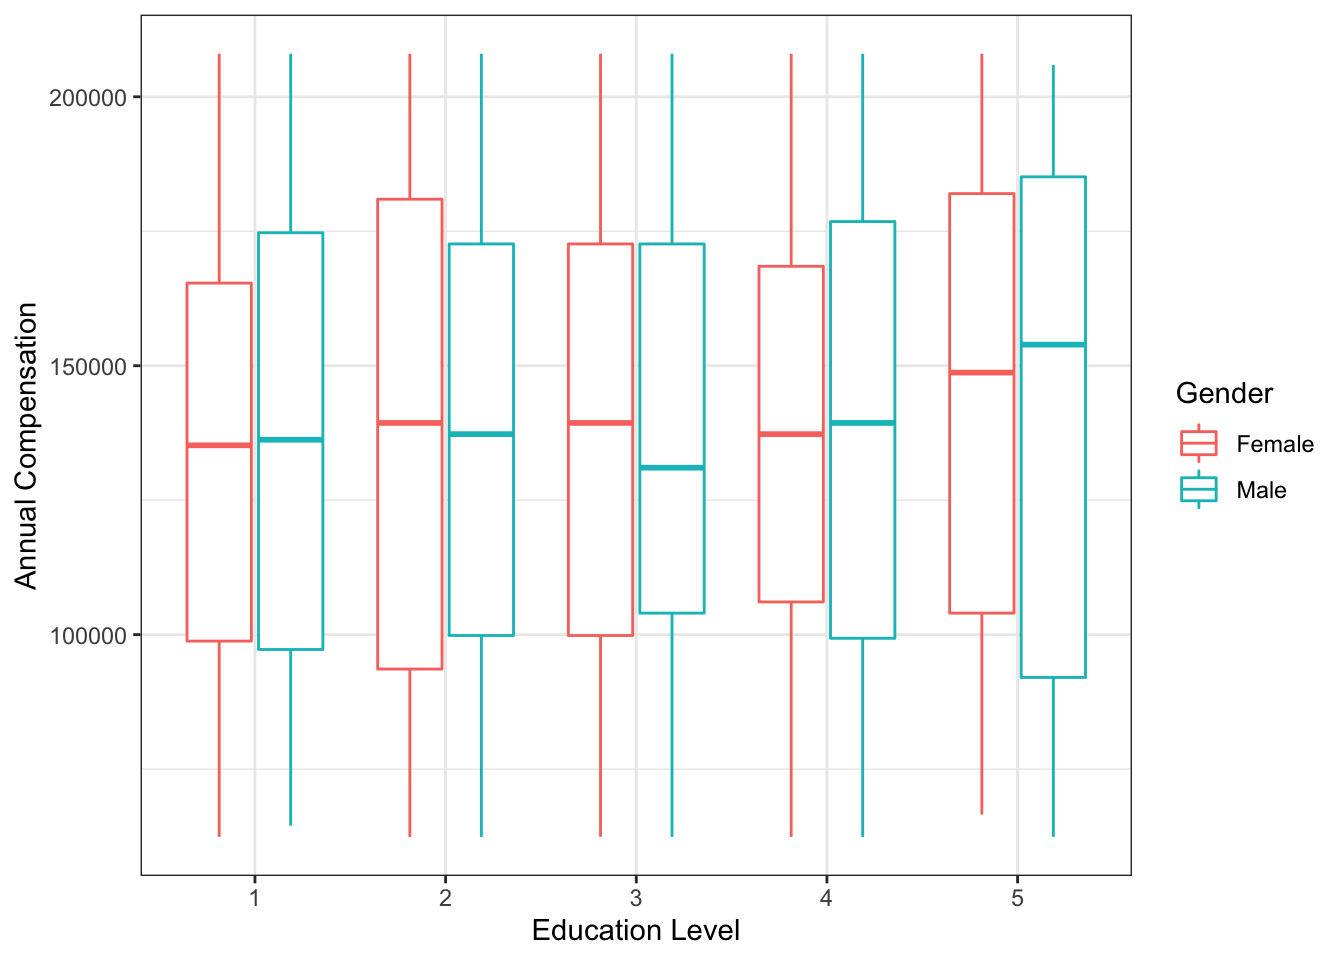
\includegraphics{People_Analytics_Lifecycle_files/figure-latex/unnamed-chunk-94-1.pdf}

Boxplots can be interpreted as follows:
* Horizontal lines represent median compensation values.
* The box in the middle of each distribution represents the IQR.
* The end of the line above the IQR represents the threshold for outliers in the upper range: \(Q3 + 1.5 * IQR\).
* The end of the line below the IQR represents the threshold for outliers in the lower range: \(Q1 - 1.5 * IQR\).
* Data points represent outliers: \(x > Q3 + 1.5 * IQR\) or \(x < Q1 - 1.5 * IQR\).

We can also return a specific percentile value using the \texttt{probs} argument in the \texttt{quantile()} function. For example, if we want to know the 80th percentile annual compensation value, we can execute the following:

\begin{Shaded}
\begin{Highlighting}[]
\CommentTok{\# Return 80th percentile annual compensation value}
\FunctionTok{quantile}\NormalTok{(employees}\SpecialCharTok{$}\NormalTok{annual\_comp, }\AttributeTok{probs =}\NormalTok{ .}\DecValTok{8}\NormalTok{)}
\end{Highlighting}
\end{Shaded}

\begin{verbatim}
##    80% 
## 180960
\end{verbatim}

In addition, the \texttt{summary()} function returns several common descriptive statistics for an object:

\begin{Shaded}
\begin{Highlighting}[]
\CommentTok{\# Return common descriptives}
\FunctionTok{summary}\NormalTok{(employees}\SpecialCharTok{$}\NormalTok{annual\_comp)}
\end{Highlighting}
\end{Shaded}

\begin{verbatim}
##    Min. 1st Qu.  Median    Mean 3rd Qu.    Max. 
##   62400   99840  137280  137054  174200  208000
\end{verbatim}

\textbf{Skewness}

\textbf{Skewness} is a measure of the horizontal distance between the mode and mean -- a representation of symmetric distortion. In most practical settings, data are not normally distributed. That is, the data are skewed either positively (right-tailed distribution) or negatively (left-tailed distribution). The coefficient of skewness is one of many ways in which we can ascertain the degree of skew in the data. The skewness of sample data is defined as:

\[ Sk = \frac{1}{n} \frac{\displaystyle\sum_{i=1}^{n} (x_i-\bar{x})^3}{s^3} \]

A positive skewness coefficient indicates positive skew, while a negative coefficient indicates negative skew. The order of descriptive statistics can also be leveraged to ascertain the direction of skew in the data:

\begin{itemize}
\tightlist
\item
  Positive skewness: mode \textless{} median \textless{} mean
\item
  Negative skewness: mode \textgreater{} median \textgreater{} mean
\item
  Symmetrical distribution: mode = median = mean
\end{itemize}

Figure \ref{fig:skewness} illustrates the placement of these descriptive statistics in each of the three types of distributions:

\begin{figure}

{\centering 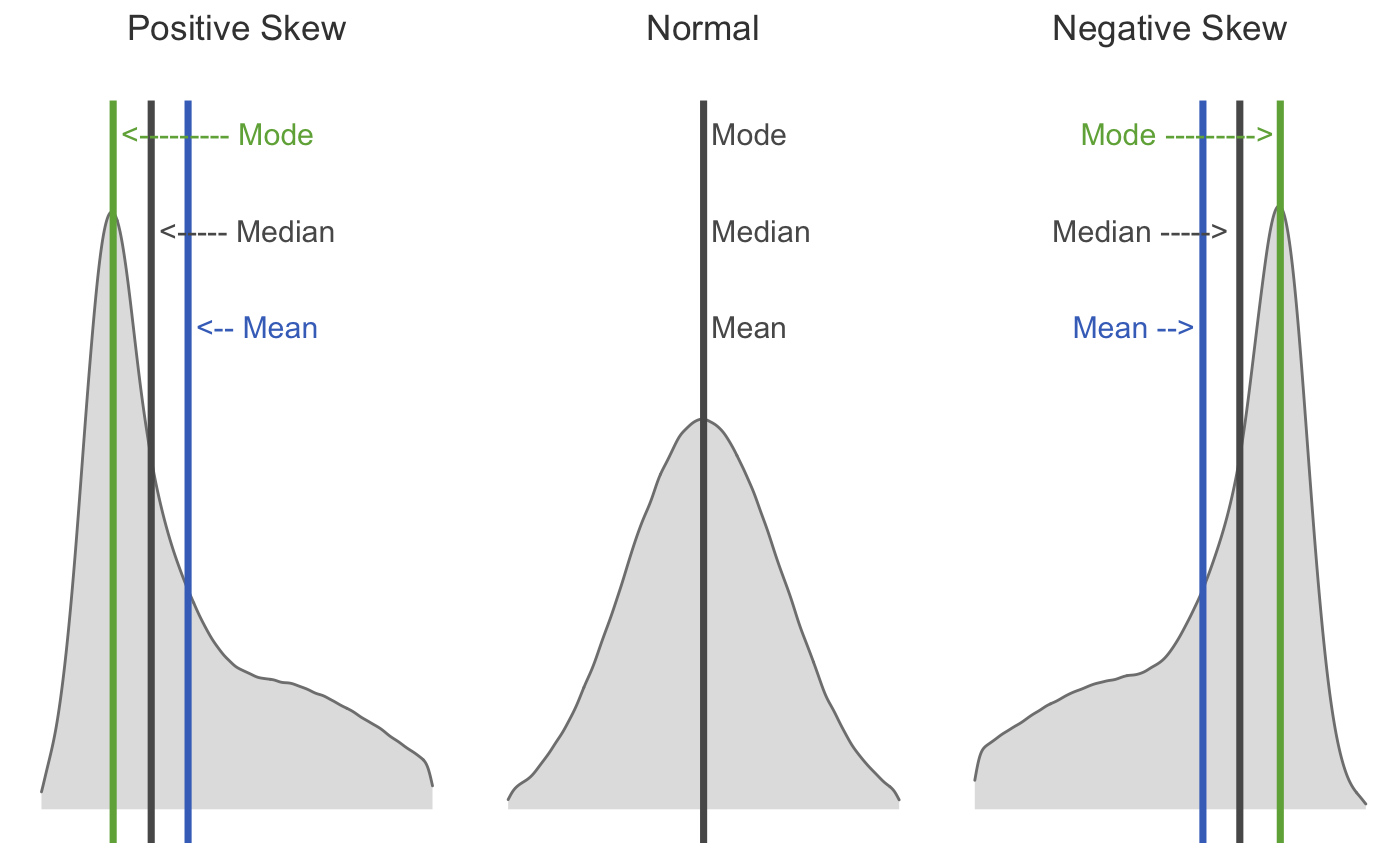
\includegraphics[width=1\linewidth]{/Users/craig.starbuck/Library/Mobile Documents/com~apple~CloudDocs/Documents/People Analytics Book/GitHub/peopleanalytics_lifecycle_book/graphics/skewness} 

}

\caption{Skewness}\label{fig:skewness}
\end{figure}

The magnitude of skewness can be determined by measuring the distance between the mode and mean relative to the variable's scale. Alternatively, we can simply evaluate this using the coefficient of skewness:

\begin{itemize}
\tightlist
\item
  If skewness is between -0.5 - 0.5, the data are considered symmetrical.
\item
  If skewness is between -0.5 and -1 or 0.5 and 1, the data are moderately skewed.
\item
  If skewness is \textless{} -1 or \textgreater{} 1, the data are highly skewed.
\end{itemize}

Since there is not a base R function for skewness, we can leverage the moments library to calculate skewness:

\begin{Shaded}
\begin{Highlighting}[]
\CommentTok{\# Load library}
\FunctionTok{library}\NormalTok{(moments)}

\CommentTok{\# Calculate skewness for org tenure, rounded to two significant figures via the round() function}
\FunctionTok{round}\NormalTok{(moments}\SpecialCharTok{::}\FunctionTok{skewness}\NormalTok{(employees}\SpecialCharTok{$}\NormalTok{org\_tenure), }\DecValTok{2}\NormalTok{)}
\end{Highlighting}
\end{Shaded}

\begin{verbatim}
## [1] 2.27
\end{verbatim}

\textbf{Statistical Moments}, after which this library was named, play an important role in specifying the appropriate probability distribution for a set of data. Moments are a set of statistical parameters used to describe the characteristics of a distribution. Skewness is the third statistical moment in the set; hence the sum of cubed differences and cubic polynomial in the denominator of the formula above. The complete set of moments comprises: (1) expected value or mean, (2) variance and standard deviation, (3) skewness, and (4) kurtosis.

We can verify that the \texttt{skewness()} function from the moments library returns the expected value (per the aforementioned formula) by validating against a manual calculation:

\begin{Shaded}
\begin{Highlighting}[]
\CommentTok{\# Store components of skewness calculation}
\NormalTok{n }\OtherTok{=} \FunctionTok{length}\NormalTok{(employees}\SpecialCharTok{$}\NormalTok{org\_tenure)}
\NormalTok{x }\OtherTok{=}\NormalTok{ employees}\SpecialCharTok{$}\NormalTok{org\_tenure}
\NormalTok{x\_bar }\OtherTok{=} \FunctionTok{mean}\NormalTok{(employees}\SpecialCharTok{$}\NormalTok{org\_tenure)}
\NormalTok{s }\OtherTok{=} \FunctionTok{sd}\NormalTok{(employees}\SpecialCharTok{$}\NormalTok{org\_tenure)}

\CommentTok{\# Calculate skewness manually, rounded to two significant figures via the round() function}
\FunctionTok{round}\NormalTok{(}\DecValTok{1}\SpecialCharTok{/}\NormalTok{n }\SpecialCharTok{*}\NormalTok{ (}\FunctionTok{sum}\NormalTok{((x }\SpecialCharTok{{-}}\NormalTok{ x\_bar)}\SpecialCharTok{\^{}}\DecValTok{3}\NormalTok{) }\SpecialCharTok{/}\NormalTok{ s}\SpecialCharTok{\^{}}\DecValTok{3}\NormalTok{), }\DecValTok{2}\NormalTok{)}
\end{Highlighting}
\end{Shaded}

\begin{verbatim}
## [1] 2.27
\end{verbatim}

A skewness coefficient of 2.27 indicates that organization tenure is positively skewed. We can visualize the data to confirm the expected right-tailed distribution:

\begin{Shaded}
\begin{Highlighting}[]
\CommentTok{\# Produce histogram to visualize sample distribution}
\NormalTok{ggplot2}\SpecialCharTok{::}\FunctionTok{ggplot}\NormalTok{() }\SpecialCharTok{+} 
\NormalTok{ggplot2}\SpecialCharTok{::}\FunctionTok{aes}\NormalTok{(employees}\SpecialCharTok{$}\NormalTok{org\_tenure) }\SpecialCharTok{+} 
\NormalTok{ggplot2}\SpecialCharTok{::}\FunctionTok{labs}\NormalTok{(}\AttributeTok{x =} \StringTok{"Organization Tenure"}\NormalTok{, }\AttributeTok{y =} \StringTok{"Density"}\NormalTok{) }\SpecialCharTok{+} 
\NormalTok{ggplot2}\SpecialCharTok{::}\FunctionTok{geom\_histogram}\NormalTok{(}\FunctionTok{aes}\NormalTok{(}\AttributeTok{y =}\NormalTok{ ..density..), }\AttributeTok{fill =} \StringTok{"\#414141"}\NormalTok{) }\SpecialCharTok{+}
\NormalTok{ggplot2}\SpecialCharTok{::}\FunctionTok{geom\_density}\NormalTok{(}\AttributeTok{fill =} \StringTok{"\#ADD8E6"}\NormalTok{, }\AttributeTok{alpha =} \FloatTok{0.6}\NormalTok{) }\SpecialCharTok{+}
\NormalTok{ggplot2}\SpecialCharTok{::}\FunctionTok{theme\_bw}\NormalTok{()}
\end{Highlighting}
\end{Shaded}

\begin{figure}

{\centering 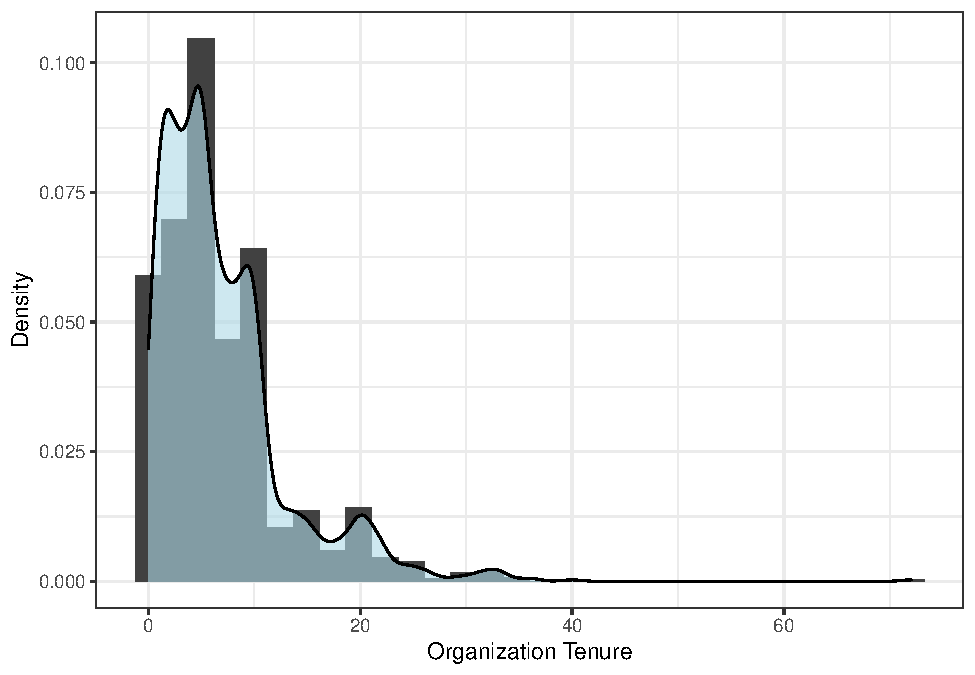
\includegraphics{People_Analytics_Lifecycle_files/figure-latex/org-tenure-distribution-1} 

}

\caption{Organization Tenure Distribution}\label{fig:org-tenure-distribution}
\end{figure}

\textbf{Kurtosis}

While skewness provides information on the symmetry of a distribution, \textbf{kurtosis} provides information on the heaviness of a distribution's tails (``tailedness''). Kurtosis is the fourth statistical moment, defined by:

\[ K = \frac{1}{n} \frac{\displaystyle\sum_{i=1}^{n} (x_i-\bar{x})^4}{s^4} \]

Note that the quartic functions characteristic of the fourth statistical moment are the only differences from the skewness formula we reviewed in the prior section (which featured cubic functions).

The terms \textbf{leptokurtic} and \textbf{platykurtic} are often used to describe distributions with light and heavy tails, respectively. ``Platy-'' in platykurtic is the same root as ``platypus'', and I've found it helpful to recall the characteristics of the flat platypus when characterizing frequency distributions as platkurtic (wide and flat) vs.~its antithesis, leptokurtic (tall and skinny). The normal (or Gaussian) distribution is referred to as a \textbf{mesokurtic} distribution in the context of kurtosis.

Figure \ref{fig:kurtosis} illustrates the three kurtosis categorizations:

\begin{figure}

{\centering 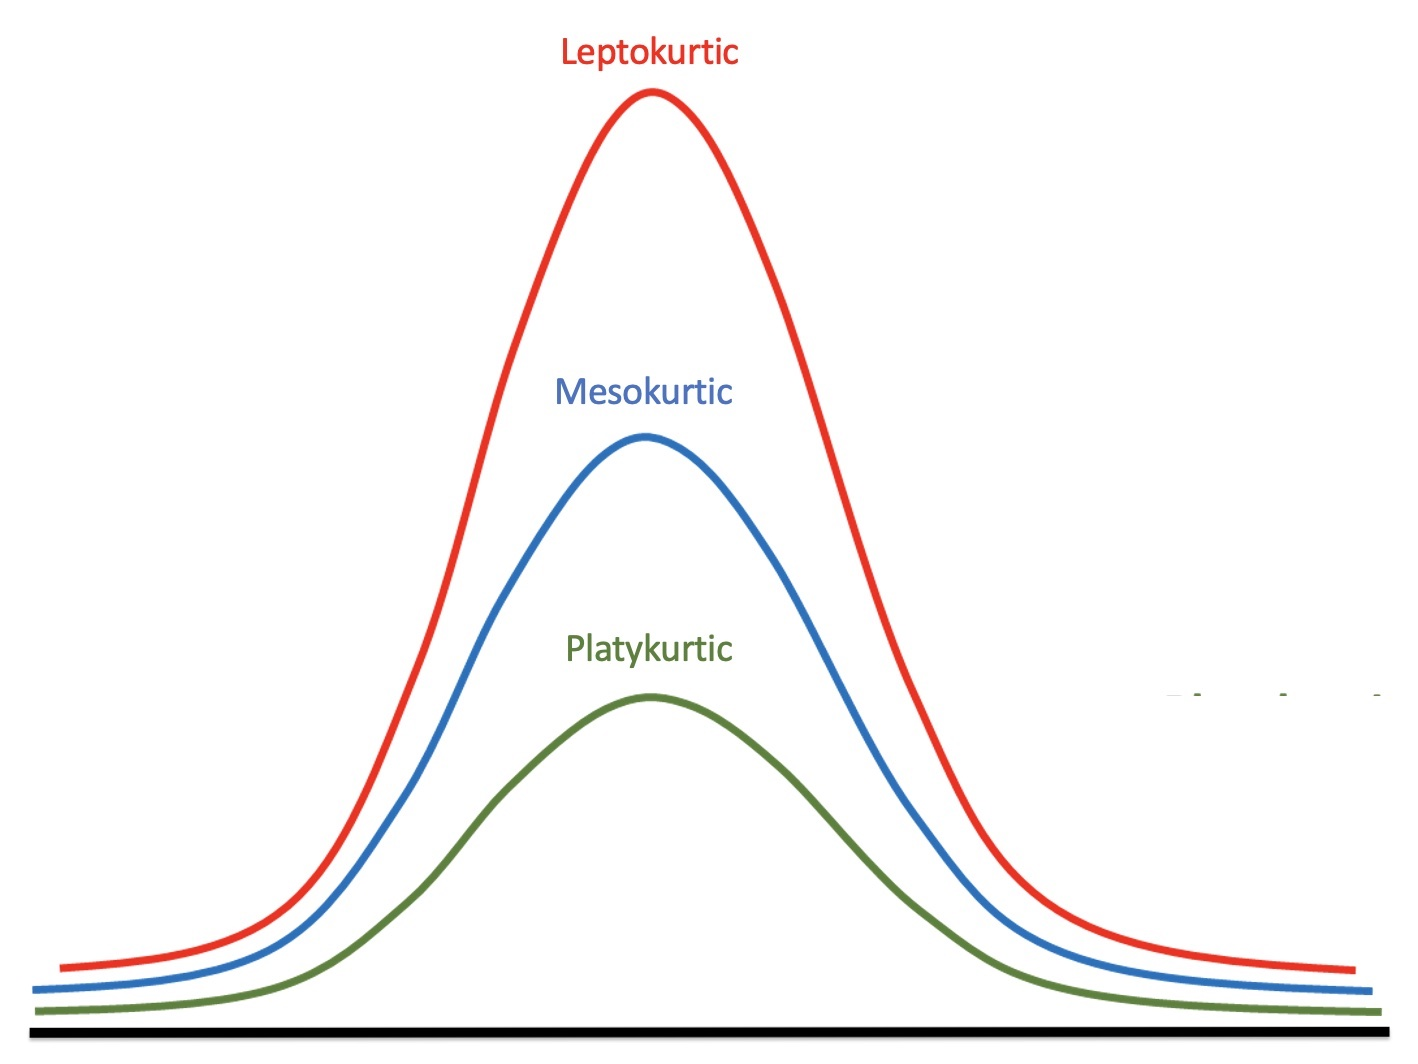
\includegraphics[width=0.75\linewidth]{/Users/craig.starbuck/Library/Mobile Documents/com~apple~CloudDocs/Documents/People Analytics Book/GitHub/peopleanalytics_lifecycle_book/graphics/kurtosis} 

}

\caption{Kurtosis}\label{fig:kurtosis}
\end{figure}

Kurtosis is measured relative to a normal distribution. Normal distributions have a kurtosis coefficient of 3. Therefore, the kurtosis coefficient is greater than 3 for leptokurtic distributions and less than 3 for platykurtic distributions.

The moments library can also be used to calculate kurtosis in R:

\begin{Shaded}
\begin{Highlighting}[]
\CommentTok{\# Calculate kurtosis for org tenure, rounded to one significant figure}
\FunctionTok{round}\NormalTok{(moments}\SpecialCharTok{::}\FunctionTok{kurtosis}\NormalTok{(employees}\SpecialCharTok{$}\NormalTok{org\_tenure), }\DecValTok{1}\NormalTok{)}
\end{Highlighting}
\end{Shaded}

\begin{verbatim}
## [1] 13.4
\end{verbatim}

We can verify that the \texttt{kurtosis()} function returns the expected value (per the aforementioned formula) by validating against a manual calculation:

\begin{Shaded}
\begin{Highlighting}[]
\CommentTok{\# Calculate kurtosis manually, rounded to one significant figure}
\FunctionTok{round}\NormalTok{(}\DecValTok{1}\SpecialCharTok{/}\NormalTok{n }\SpecialCharTok{*}\NormalTok{ (}\FunctionTok{sum}\NormalTok{((x }\SpecialCharTok{{-}}\NormalTok{ x\_bar)}\SpecialCharTok{\^{}}\DecValTok{4}\NormalTok{) }\SpecialCharTok{/}\NormalTok{ s}\SpecialCharTok{\^{}}\DecValTok{4}\NormalTok{), }\DecValTok{1}\NormalTok{)}
\end{Highlighting}
\end{Shaded}

\begin{verbatim}
## [1] 13.4
\end{verbatim}

Our kurtosis coefficient of 13.4 indicates a leptokurtic distribution which is supported by the visual in Figure \ref{fig:org-tenure-distribution}.

It is important not to characterize a distribution based on a single isolated metric; we need the complete set of statistical moments to fully understand the distribution of data.

\hypertarget{bivariate-analysis}{%
\section{Bivariate Analysis}\label{bivariate-analysis}}

While univariate analysis explores each variable independently, \textbf{bivariate analysis} explores statistical relationships between two variables.

\hypertarget{covariance}{%
\subsection{Covariance}\label{covariance}}

While variance provides an understanding of how values for a single variable vary, \textbf{covariance} is an unstandardized measure of how two variables vary together. Values can range from \(-\infty\) to \(+\infty\), and these values can be used to understand the direction of the linear relationship between variables. Positive covariance values indicate that the variables vary in the same direction (e.g., tend to increase or decrease together), while negative covariance values indicate that the variables vary in opposite directions (e.g., when one increases, the other decreases, or vice versa).

Covariance of a sample is defined by:

\[ cov_{x,y} = \frac{\displaystyle\sum_{i=1}^{n} (x_{i}-\bar{x})(y_{i}-\bar{y})}{n-1} \]

It's important to note that while covariance aids our understanding of the direction of the relationship between two variables, we cannot use it to understand the strength of the association since it is unstandardized. Due to differences in variables' units of measurement, the strength of the relationship between two variables with large covariance could be weak, while the strength of the relationship between another pair of variables with small covariance could be strong.

In R, we can compute the covariance between a pair of numeric variables by passing the two vectors into the \texttt{cov()} function:

\begin{Shaded}
\begin{Highlighting}[]
\CommentTok{\# Calculate sample covariance between annual compensation and age using complete observations (missing values will cause issues if not addressed)}
\FunctionTok{cov}\NormalTok{(employees}\SpecialCharTok{$}\NormalTok{annual\_comp, employees}\SpecialCharTok{$}\NormalTok{age, }\AttributeTok{use =} \StringTok{"complete.obs"}\NormalTok{)}
\end{Highlighting}
\end{Shaded}

\begin{verbatim}
## [1] 9381.677
\end{verbatim}

In this example, using the default Pearson method, the covariance between annual compensation and age is 9,381.7. The positive value indicates that annual compensation is generally higher for older employees and lower for younger employees.

Just as we multiplied the sample variance by \((n - 1) / n\) to obtain the population variance, we can apply the same approach to convert the sample covariance returned by \texttt{cov()} to the population covariance:

\begin{Shaded}
\begin{Highlighting}[]
\CommentTok{\# Calculate population covariance between annual compensation and age}
\FunctionTok{cov}\NormalTok{(employees}\SpecialCharTok{$}\NormalTok{annual\_comp, employees}\SpecialCharTok{$}\NormalTok{age, }\AttributeTok{use =} \StringTok{"complete.obs"}\NormalTok{) }\SpecialCharTok{*}\NormalTok{ (n }\SpecialCharTok{{-}} \DecValTok{1}\NormalTok{) }\SpecialCharTok{/}\NormalTok{ n}
\end{Highlighting}
\end{Shaded}

\begin{verbatim}
## [1] 9375.295
\end{verbatim}

The examples thus far have only examined associations between two variables at a time. However, rather than looking at isolated pairwise relationships, we can produce a covariance matrix to surface associations among many variables by passing a dataframe or matrix object into the \texttt{cov()} function:

\begin{Shaded}
\begin{Highlighting}[]
\CommentTok{\# Generate a covariance matrix among select continuous variables}
\FunctionTok{cov}\NormalTok{(}\FunctionTok{subset}\NormalTok{(employees, }\AttributeTok{select =} \FunctionTok{c}\NormalTok{(}\StringTok{"annual\_comp"}\NormalTok{, }\StringTok{"age"}\NormalTok{, }\StringTok{"org\_tenure"}\NormalTok{, }\StringTok{"job\_tenure"}\NormalTok{, }\StringTok{"prior\_emplr\_cnt"}\NormalTok{, }\StringTok{"commute\_dist"}\NormalTok{)), }\AttributeTok{use =} \StringTok{"complete.obs"}\NormalTok{)}
\end{Highlighting}
\end{Shaded}

\begin{verbatim}
##                   annual_comp          age    org_tenure    job_tenure
## annual_comp      1.788039e+09 9381.6772019 -3921.9601469 -3693.1960749
## age              9.381677e+03   83.4550488    17.9255146     7.0467503
## org_tenure      -3.921960e+03   17.9255146    39.7967987    16.9797312
## job_tenure      -3.693196e+03    7.0467503    16.9797312    13.1271220
## prior_emplr_cnt  2.340406e+03    6.8377387    -1.8547177    -0.8213802
## commute_dist     1.067158e+04   -0.1248728     0.7746438     0.5535206
##                 prior_emplr_cnt  commute_dist
## annual_comp        2340.4057552 10671.5790741
## age                   6.8377387    -0.1248728
## org_tenure           -1.8547177     0.7746438
## job_tenure           -0.8213802     0.5535206
## prior_emplr_cnt       6.2400490    -0.5923586
## commute_dist         -0.5923586    65.7212510
\end{verbatim}

Using the default Pearson method, the \texttt{cov()} function will return sample variances for each variable down the diagonal, since covariance is not applicable in the context of a variable with itself. We can confirm by producing the variance for age:

\begin{Shaded}
\begin{Highlighting}[]
\CommentTok{\# Return sample variance for age}
\FunctionTok{var}\NormalTok{(employees}\SpecialCharTok{$}\NormalTok{age)}
\end{Highlighting}
\end{Shaded}

\begin{verbatim}
## [1] 83.45505
\end{verbatim}

As expected, the variance for age (\(s^{2} = 83.5\)) matches the value found in the age x age cell of the covariance matrix.

\hypertarget{correlation}{%
\subsection{Correlation}\label{correlation}}

\textbf{Correlation} is a scaled form of covariance. While covariance provides an unstandardized measure of the direction of a relationship between variables, correlation provides a standardized measure that can be used to quantify both the direction and strength of bivariate relationships. Correlation coefficients range from -1 to 1, where -1 indicates a perfectly negative association, 1 indicates a perfectly positive association, and 0 indicates the absence of an association. \textbf{Pearson's product-moment correlation coefficient} \(r\) is defined by:

\[ r_{x,y} = \frac{\displaystyle\sum_{i=1}^{n} (x_{i}-\bar{x})(y_{i}-\bar{y})}{\sqrt{\displaystyle\sum_{i=1}^{n} (x_{i}-\bar{x})^2 \displaystyle\sum_{i=1}^{n} (y_{i}-\bar{y})^2}} \]

In R, Pearson's \(r\) can be calculated using the \texttt{cor()} function:

\begin{Shaded}
\begin{Highlighting}[]
\CommentTok{\# Calculate the correlation between annual compensation and age}
\FunctionTok{cor}\NormalTok{(employees}\SpecialCharTok{$}\NormalTok{annual\_comp, employees}\SpecialCharTok{$}\NormalTok{age, }\AttributeTok{use =} \StringTok{"complete.obs"}\NormalTok{)}
\end{Highlighting}
\end{Shaded}

\begin{verbatim}
## [1] 0.02428654
\end{verbatim}

While we already know that the relationship between annual compensation and age is positive based on the positive covariance coefficient, Pearson's \(r\) of .02 indicates that the strength of the positive association is weak (\(r\) = 0 represents the absence of a relationship). Though there are no absolute rules for categorizing the strength of relationships, as thresholds often vary by domain, the following is a general rule of thumb for interpreting the strength of bivariate associations:

\begin{itemize}
\tightlist
\item
  Weak = Absolute value of correlation coefficients between 0 and .3
\item
  Moderate = Absolute value of correlation coefficients between .4 and .6
\item
  Strong = Absolute value of correlation coefficients between .7 and 1
\end{itemize}

There are several correlation coefficients, and the measurement scale of \(x\) and \(y\) determine the appropriate type:

\begin{figure}

{\centering 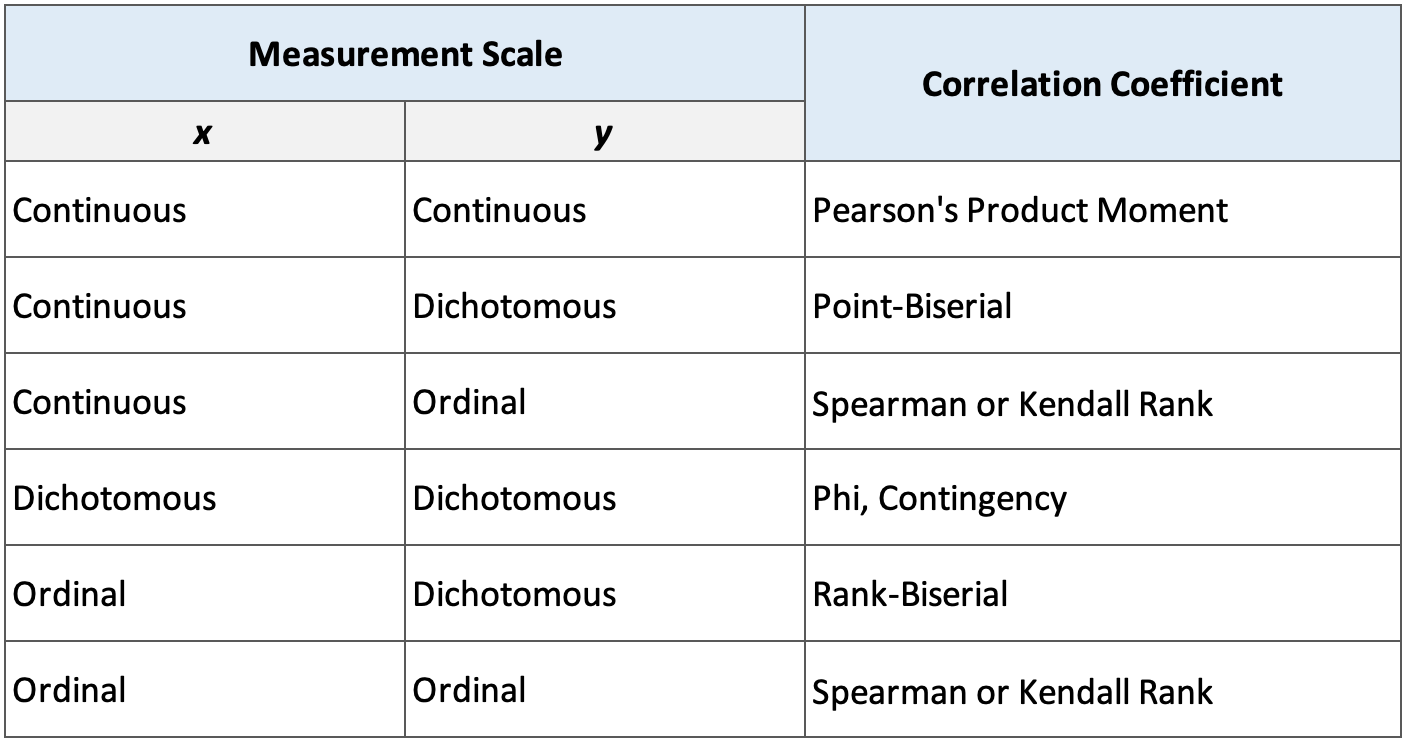
\includegraphics[width=1\linewidth]{/Users/craig.starbuck/Library/Mobile Documents/com~apple~CloudDocs/Documents/People Analytics Book/GitHub/peopleanalytics_lifecycle_book/graphics/correlation_table} 

}

\caption{Proper Applications of Correlation Coefficients}\label{fig:corr-table}
\end{figure}

Pearson's \(r\) can be used when both variables are measured on continuous scales or when one is continuous and the other is dichotomous (point-biserial correlation).

When one or both variables are ordinal, we can leverage \textbf{Spearman's} \(\rho\) or \textbf{Kendall's} \(\tau\), which are both standardized nonparametric measures of the association between one or two rank-ordered variables. Let's look at Spearman's \(\rho\), which is defined as:

\[ \rho = 1 - {\frac {6 \sum d_i^2}{n(n^2 - 1)}} \]

We can override the default Pearson method in the \texttt{cor()} function to implement a specific form of rank correlation using the \texttt{method} argument:

\begin{Shaded}
\begin{Highlighting}[]
\CommentTok{\# Calculate the correlation between job level and education level using Spearman\textquotesingle{}s method}
\FunctionTok{cor}\NormalTok{(employees}\SpecialCharTok{$}\NormalTok{job\_lvl, employees}\SpecialCharTok{$}\NormalTok{ed\_lvl, }\AttributeTok{method =} \StringTok{"spearman"}\NormalTok{, }\AttributeTok{use =} \StringTok{"complete.obs"}\NormalTok{)}
\end{Highlighting}
\end{Shaded}

\begin{verbatim}
## [1] 0.1074192
\end{verbatim}

The \(\rho\) coefficient of .11 indicates that the positive association between job level and education level is weak. We could also pass \texttt{method\ =\ "kendall"} to this \texttt{cor()} function to implement Kendall's \(\tau\).

The \textbf{Phi Coefficient} (\(\phi\)), sometimes referred to as the mean square contingency coefficient or Matthews correlation in ML, can be used to understand the association between two dichotomous variables. For a 2x2 table for two random variables \(x\) and \(y\):

\begin{figure}

{\centering 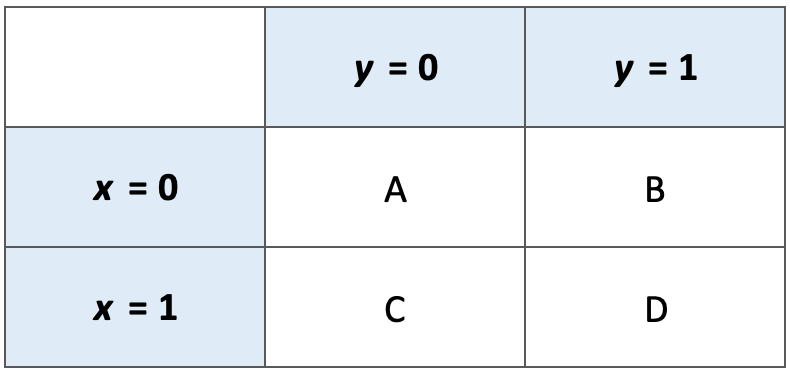
\includegraphics[width=0.5\linewidth]{/Users/craig.starbuck/Library/Mobile Documents/com~apple~CloudDocs/Documents/People Analytics Book/GitHub/peopleanalytics_lifecycle_book/graphics/phi_coefficient_formula} 

}

\caption{2x2 Table for Random Variables x and y}\label{fig:phi-tbl}
\end{figure}

The \(\phi\) coefficient is defined as:

\[ \phi = {\frac {(AD-BC)}{\sqrt{(A+B)(C+D)(A+C)(B+D)}}} \]

To illustrate, let's examine whether there is a relationship between gender and performance after transforming performance from its ordinal form to a dichotomous variable (high vs.~low performance). We can leverage the \texttt{psych} library to calculate \(\phi\) in R:

\begin{Shaded}
\begin{Highlighting}[]
\CommentTok{\# Set females to 1 and everything else to 0}
\NormalTok{employees}\SpecialCharTok{$}\NormalTok{gender\_code }\OtherTok{\textless{}{-}} \FunctionTok{ifelse}\NormalTok{(employees}\SpecialCharTok{$}\NormalTok{gender }\SpecialCharTok{==} \StringTok{\textquotesingle{}Female\textquotesingle{}}\NormalTok{, }\DecValTok{1}\NormalTok{, }\DecValTok{0}\NormalTok{)}

\CommentTok{\# Set stock options to 1 if level \textgreater{} 0}
\NormalTok{employees}\SpecialCharTok{$}\NormalTok{stock\_option\_code }\OtherTok{\textless{}{-}} \FunctionTok{ifelse}\NormalTok{(employees}\SpecialCharTok{$}\NormalTok{stock\_opt\_lvl }\SpecialCharTok{\textgreater{}} \DecValTok{0}\NormalTok{, }\DecValTok{1}\NormalTok{, }\DecValTok{0}\NormalTok{)}

\CommentTok{\# Create a 2x2 contingency table}
\NormalTok{contingency\_tbl }\OtherTok{\textless{}{-}} \FunctionTok{table}\NormalTok{(employees}\SpecialCharTok{$}\NormalTok{gender\_code, employees}\SpecialCharTok{$}\NormalTok{stock\_option\_code)}

\CommentTok{\# Calculate the Phi Coefficient between dichotomous variables}
\NormalTok{psych}\SpecialCharTok{::}\FunctionTok{phi}\NormalTok{(contingency\_tbl)}
\end{Highlighting}
\end{Shaded}

\begin{verbatim}
## [1] -0.01
\end{verbatim}

\(\phi\) is essentially 0, which means stock options are distributed equitably across gender categories (good news!). While there are not differences in the proportion of males and females who receive at least some stock options, examining whether there is equity in the amount of stock grants and refreshes may be a good next step.

A correlation matrix can be produced to surface associations among many variables by passing a dataframe or matrix object into the \texttt{cor()} function:

\begin{Shaded}
\begin{Highlighting}[]
\CommentTok{\# Generate a correlation matrix among select continuous variables}
\FunctionTok{cor}\NormalTok{(}\FunctionTok{subset}\NormalTok{(employees, }\AttributeTok{select =} \FunctionTok{c}\NormalTok{(}\StringTok{"annual\_comp"}\NormalTok{, }\StringTok{"age"}\NormalTok{, }\StringTok{"org\_tenure"}\NormalTok{, }\StringTok{"job\_tenure"}\NormalTok{, }\StringTok{"prior\_emplr\_cnt"}\NormalTok{, }\StringTok{"commute\_dist"}\NormalTok{)), }\AttributeTok{use =} \StringTok{"complete.obs"}\NormalTok{)}
\end{Highlighting}
\end{Shaded}

\begin{verbatim}
##                 annual_comp         age  org_tenure  job_tenure prior_emplr_cnt
## annual_comp      1.00000000  0.02428654 -0.01470248 -0.02410622      0.02215688
## age              0.02428654  1.00000000  0.31104359  0.21290106      0.29963476
## org_tenure      -0.01470248  0.31104359  1.00000000  0.74288567     -0.11769547
## job_tenure      -0.02410622  0.21290106  0.74288567  1.00000000     -0.09075393
## prior_emplr_cnt  0.02215688  0.29963476 -0.11769547 -0.09075393      1.00000000
## commute_dist     0.03113059 -0.00168612  0.01514695  0.01884500     -0.02925080
##                 commute_dist
## annual_comp       0.03113059
## age              -0.00168612
## org_tenure        0.01514695
## job_tenure        0.01884500
## prior_emplr_cnt  -0.02925080
## commute_dist      1.00000000
\end{verbatim}

Based on this correlation matrix, most pairwise associations are weak with the exception of the relationship between \texttt{org\_tenure} and \texttt{job\_tenure} (\(r = .7\)). The values down the diagonal are 1 because these represent the correlation between each variable with itself. You may also notice that the information above and below the diagonal is identical and, therefore, redundant.

A great R library for visualizing correlation matrices is corrplot. Several arguments can be specified for various visual representations of the relationships among variables:

\begin{figure}

{\centering 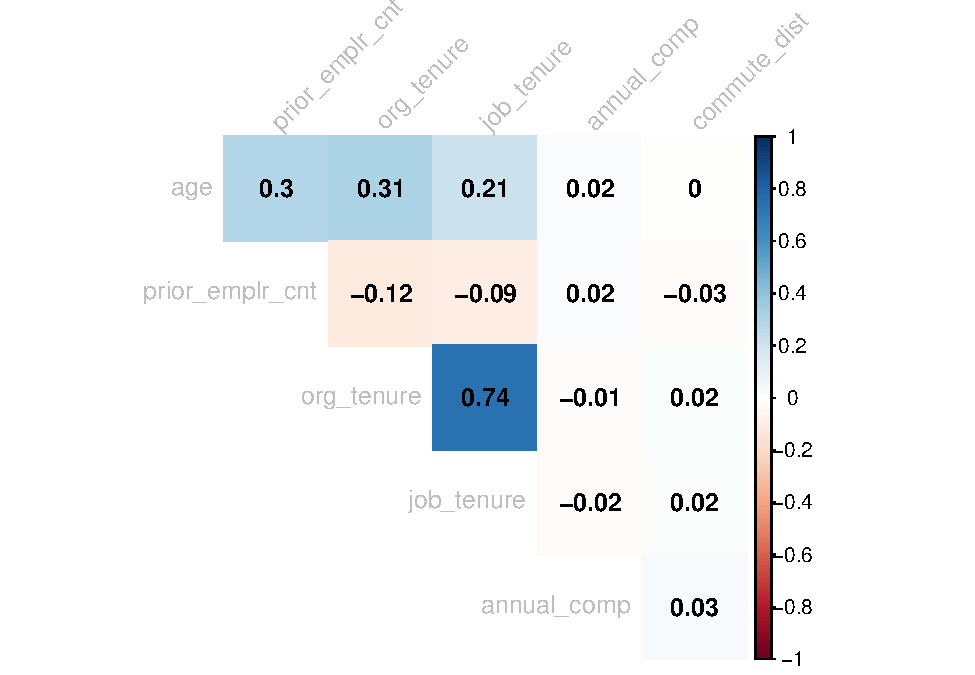
\includegraphics[width=1\linewidth]{People_Analytics_Lifecycle_files/figure-latex/corrplot-comp-1} 

}

\caption{Corrplot correlation matrix}\label{fig:corrplot-comp}
\end{figure}

The GGally library produces a variety of useful information, including correlation coefficients, bivariate scatterplots, and univariate distributions:

\begin{figure}

{\centering 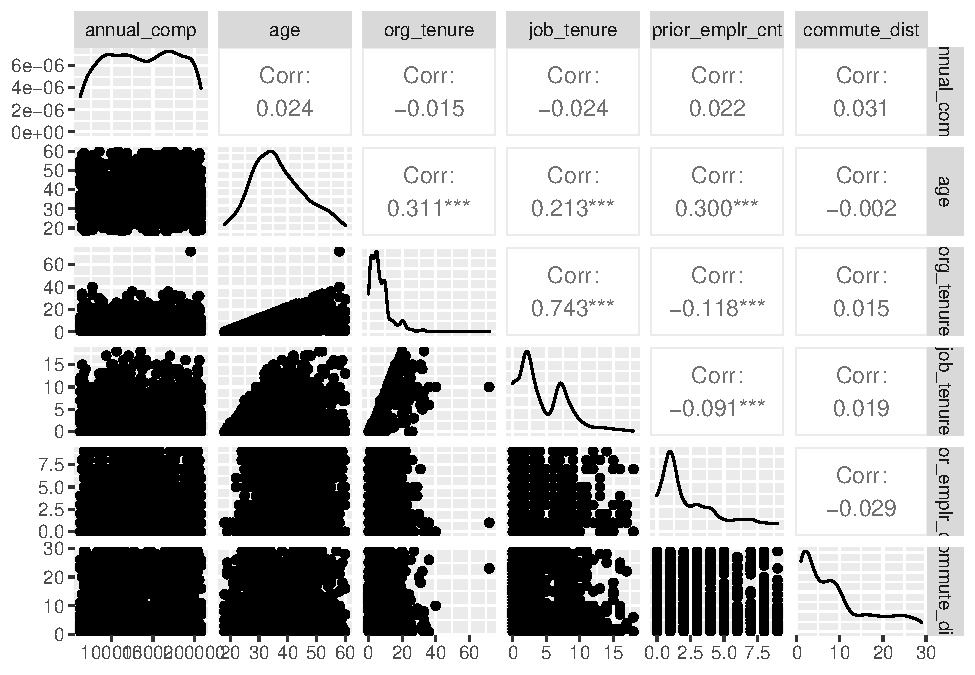
\includegraphics[width=1\linewidth]{People_Analytics_Lifecycle_files/figure-latex/ggpairs-comp-1} 

}

\caption{GGpairs bivariate correlations and data distributions.}\label{fig:ggpairs-comp}
\end{figure}

We may find that these bivariate associations look quite different for certain business areas or jobs, assuming departments and jobs were created at different points in the company's history. There is often a lot of noise in data at the broader company level, so understanding the nature and nuance of associations will be highly important. We will explore this further in the context of linear regression in Chapter \ref{lm}.

It's important to remember that correlation is not causation. Correlations can be spurious (variables related by chance), and drawing conclusions based on bivariate associations alone -- especially in the absence of sound theoretical underpinnings -- can be dangerous.

\begin{figure}

{\centering 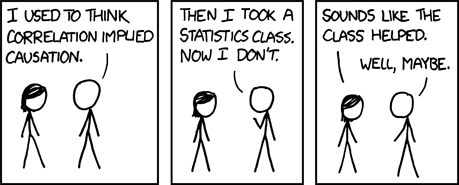
\includegraphics[width=0.75\linewidth]{/Users/craig.starbuck/Library/Mobile Documents/com~apple~CloudDocs/Documents/People Analytics Book/GitHub/peopleanalytics_lifecycle_book/graphics/correlation_comic} 

}

\caption{Correlation comic (Source: www.explainxkcd.com)}\label{fig:corr-comic}
\end{figure}

Here are two examples of nearly perfect correlations between variables for which there is likely no true direct association:

\begin{figure}

{\centering 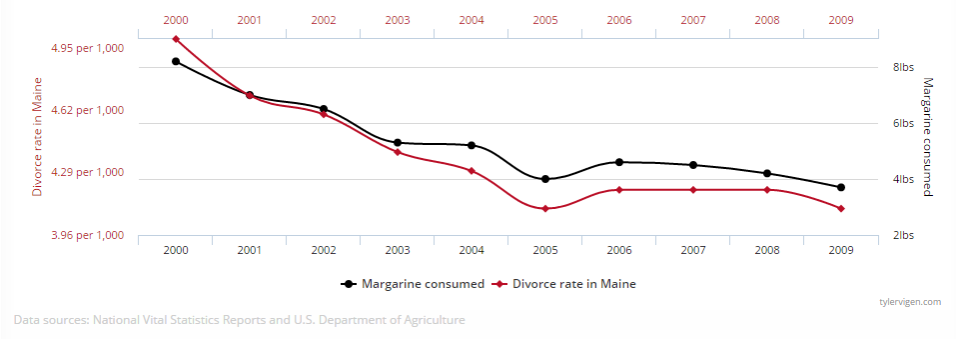
\includegraphics[width=1\linewidth]{/Users/craig.starbuck/Library/Mobile Documents/com~apple~CloudDocs/Documents/People Analytics Book/GitHub/peopleanalytics_lifecycle_book/graphics/spurious_corr_maine_divorce} 

}

\caption{Correlation between Maine Divorce Rate and Margarine Consumption (r = .99)}\label{fig:spur-corr-1}
\end{figure}

\begin{figure}

{\centering 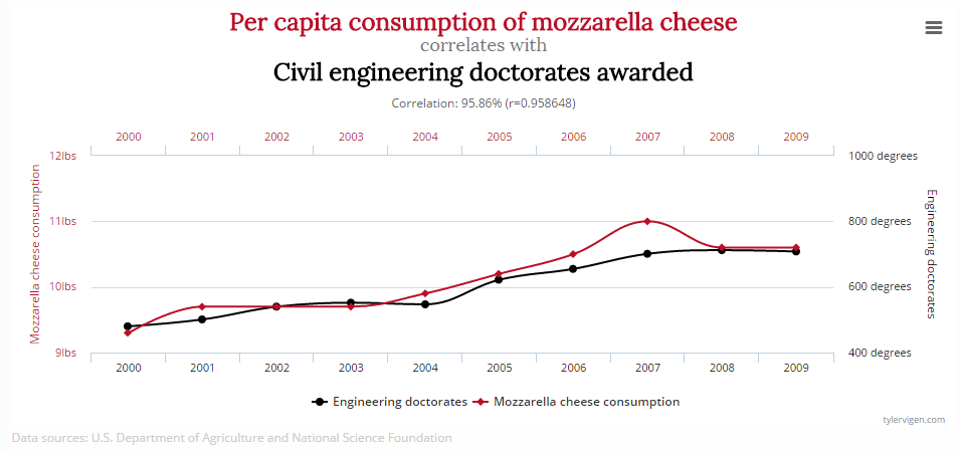
\includegraphics[width=1\linewidth]{/Users/craig.starbuck/Library/Mobile Documents/com~apple~CloudDocs/Documents/People Analytics Book/GitHub/peopleanalytics_lifecycle_book/graphics/spurious_corr_mozzarella_cheese} 

}

\caption{Correlation between Mozzarella Cheese Consumption and Civil Engineering Doctorate Conferrals (r = .96)}\label{fig:spur-corr-2}
\end{figure}

In addition, covariance and correlation alone are not sufficient for determining whether an observed association in sample data is also present in the population. To understand the likelihood that patterns observed in sample data are also present in the larger population of interest, we need to move beyond descriptive measures.

\hypertarget{review-questions-4}{%
\section{Review Questions}\label{review-questions-4}}

\begin{enumerate}
\def\labelenumi{\arabic{enumi}.}
\item
  How does the mean and median compare with respect to sensitivity to extreme values (outliers)?
\item
  What does the standard deviation tell us about the spread of data, and how does it compare to the variance?
\item
  How does the order of the mean, median, and mode differ between positively and negatively skewed distributions?
\item
  Do large covariance coefficients always indicate strong bivariate associations? Why or why not?
\item
  What information is represented in boxplots?
\item
  Do do quartiles relate to percentiles?
\item
  What type of correlation coefficient should be used when evaluating the relationship between a pair of rank-ordered variables?
\item
  What type of correlation coefficient should be used when evaluating the relationship between a pair of dichotomous variables?
\item
  How would you characterize the shape of platykurtic, leptokurtic, and mesokurtic distributions?
\item
  When using the Pearson method, what do the values down the diagonal of a \emph{covariance} matrix represent?
\end{enumerate}

\hypertarget{inf-stats}{%
\chapter{Statistical Inference}\label{inf-stats}}

The objective of \textbf{inferential statistics} is to make inferences -- with some degree of confidence -- about a population based on available sample data. Several related concepts are fundamental to this goal and will be covered here.

\hypertarget{introduction-to-probability}{%
\section{Introduction to Probability}\label{introduction-to-probability}}

Randomness and uncertainty exist all around us. In \textbf{probability theory}, random phenomena refer to events or experiments whose outcomes cannot be predicted with certainty (Pishro-Nik, 2014). If you've taken a course in probability, there is a good chance you have considered the case of a fair coin flip -- one of the most intuitive applications of probability. In the absence of information on how the coin is flipped, we cannot be certain of the outcome. What we can be certain of is that with a large number of coin flips, the proportion of heads will become increasingly close to 50\%, or \(\frac{1}{2}\).

The \textbf{Law of Large Numbers (LLN)} is an important theorem for building an intuitive understanding of how probability relates to the statistical inference concepts we will cover. In the case of a fair coin flip, it is possible to observe many consecutive heads by chance. This is because small samples can lend to anomalies. However, as the number of flips increases, we will undoubtedly observe an increasing number of tails; we expect a roughly equal number of heads and tails with a large enough number of flips.

\hypertarget{probability-distributions}{%
\subsection{Probability Distributions}\label{probability-distributions}}

\textbf{Probability distributions} are statistical functions that yield the probability of obtaining possible values for a random variable. Probabilities range from 0 to 1, where the probability of a definite event is 1 and the probability of an impossible event is 0. The \textbf{empirical probability (or experimental probability)} of an event is the fraction of times it occurred relative to the total number of repetitions. Since a probability distribution defines the likelihood of observing all possible outcomes of an event or experiment, the sum of all probabilities for all possible values must equal 1.

For example, let's look at how org tenure is distributed across employees. We can understand the general shape of the distribution using descriptive statistics:

\begin{Shaded}
\begin{Highlighting}[]
\CommentTok{\# Load library for data wrangling}
\FunctionTok{library}\NormalTok{(dplyr)}

\CommentTok{\# Read employee data}
\NormalTok{employees }\OtherTok{\textless{}{-}} \FunctionTok{read.csv}\NormalTok{(}\StringTok{"/Users/craig.starbuck/Library/Mobile Documents/com\textasciitilde{}apple\textasciitilde{}CloudDocs/Documents/People Analytics Book/GitHub/peopleanalytics\_lifecycle\_book/data/employees.csv"}\NormalTok{)}

\CommentTok{\# Produce descriptive stats for org tenure}
\FunctionTok{summary}\NormalTok{(employees}\SpecialCharTok{$}\NormalTok{org\_tenure)}
\end{Highlighting}
\end{Shaded}

\begin{verbatim}
##    Min. 1st Qu.  Median    Mean 3rd Qu.    Max. 
##   0.000   3.000   5.000   7.032   9.000  72.000
\end{verbatim}

Comparing the higher mean value of 7.03 to the median value of 5 indicates there are larger values skewing the mean upward which can be seen in the Q3 and max values.

Beyond descriptives, visuals are often helpful in understanding a variable's distribution. As shown in Figure \ref{fig:org-tenure-dist}, it is clear that org tenure is positively skewed, and understanding the shape (or spread) of this distribution enables us to identify which values are most likely in order to estimate the likelihood of different results:

\begin{Shaded}
\begin{Highlighting}[]
\CommentTok{\# Visualize org tenure distribution}
\NormalTok{ggplot2}\SpecialCharTok{::}\FunctionTok{ggplot}\NormalTok{() }\SpecialCharTok{+} 
\NormalTok{ggplot2}\SpecialCharTok{::}\FunctionTok{aes}\NormalTok{(employees}\SpecialCharTok{$}\NormalTok{org\_tenure) }\SpecialCharTok{+} 
\NormalTok{ggplot2}\SpecialCharTok{::}\FunctionTok{labs}\NormalTok{(}\AttributeTok{x =} \StringTok{"Org Tenure"}\NormalTok{, }\AttributeTok{y =} \StringTok{"Density"}\NormalTok{) }\SpecialCharTok{+} 
\NormalTok{ggplot2}\SpecialCharTok{::}\FunctionTok{geom\_histogram}\NormalTok{(}\FunctionTok{aes}\NormalTok{(}\AttributeTok{y =}\NormalTok{ ..density..), }\AttributeTok{fill =} \StringTok{"\#414141"}\NormalTok{) }\SpecialCharTok{+}
\NormalTok{ggplot2}\SpecialCharTok{::}\FunctionTok{geom\_density}\NormalTok{(}\AttributeTok{fill =} \StringTok{"\#ADD8E6"}\NormalTok{, }\AttributeTok{alpha =} \FloatTok{0.6}\NormalTok{) }\SpecialCharTok{+}
\NormalTok{ggplot2}\SpecialCharTok{::}\FunctionTok{theme\_bw}\NormalTok{()}
\end{Highlighting}
\end{Shaded}

\begin{figure}

{\centering 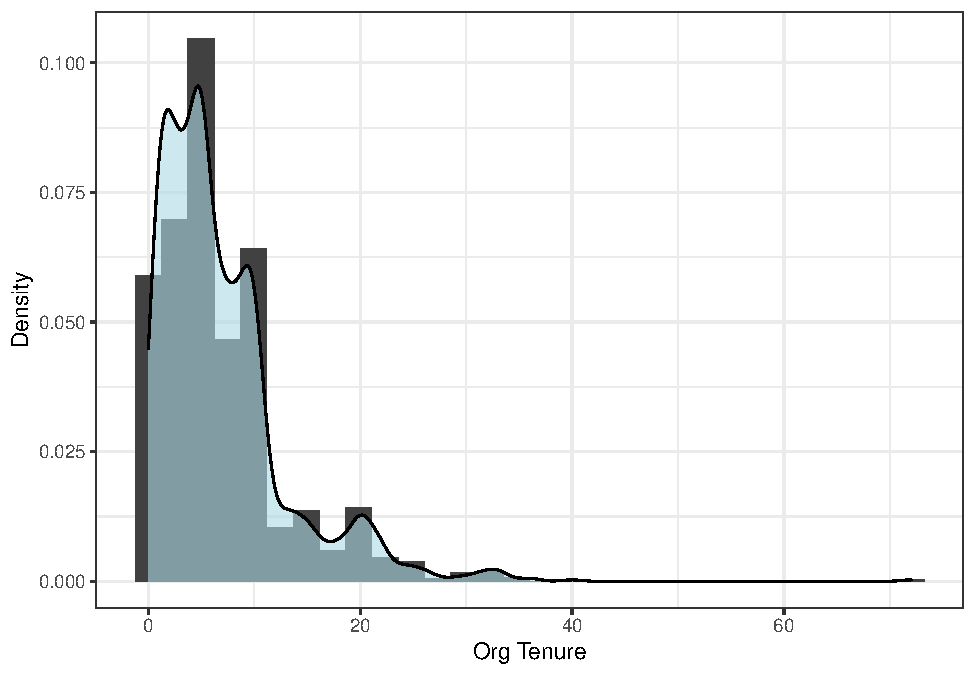
\includegraphics{People_Analytics_Lifecycle_files/figure-latex/org-tenure-dist-1} 

}

\caption{Org Tenure Distribution}\label{fig:org-tenure-dist}
\end{figure}

You can likely image the shape of probability distributions for many common events. If we consider the probability of employees exiting an organization, the outcome is binary. That is, employees either leave or stay; there are no options between these extremes. However, the distribution of performance scores will look quite different. Most organizations have expected -- or even forced -- distributions in which an average rating is awarded most frequently and low and high performance ratings less frequently. This would start to look more like a bell curve as the number of performance levels increases.

Just as we grouped variables into discrete and continuous categories in Chapter \ref{measure-sampl}, this is also how probability distributions are categorized. If you read Chapter \ref{measure-sampl}, you likely already have some a priori expectations about the characteristics of discrete and continuous distributions.

The shape of a probability distribution is defined by parameters, which represent its essential properties (e.g., measures of central tendency and spread). These probability distributions underpin the many types of statistical tests covered in this book.

\textbf{Discrete Probability Distributions}

\textbf{Discrete probability distributions}, also known as \textbf{Probability Mass Functions (PMF)}, can be leveraged to model different types of nominal and ordinal variables. Some common discrete distributions include:

\begin{itemize}
\tightlist
\item
  \textbf{Bernoulli}: probability of success or failure for a \emph{single} observation with two outcomes
\item
  \textbf{Binomial}: number of successes and failures in a \emph{sequence} of independent observations with two outcomes (collection of Bernoulli trials)
\item
  \textbf{Multinomial}: generalization of the binomial distribution for observations with more than two outcomes
\item
  \textbf{Negative Binomial (Pascal)}: a version of the binomial distribution for a \emph{fixed} number of observations (this is positively skewed despite what the name might suggest)
\item
  \textbf{Poisson}: probability of a given number of events occurring over a specified period
\item
  \textbf{Geometric}: special case of the negative binomial distribution that repeats observations until a success is observed (rather than a fixed number of times)
\end{itemize}

Several functions are available in R to simulate PMFs. The precise shape of a distribution depends on the parameters, but we will simulate and visualize these common PMFs to illustrate differences in the general shape of each. First, let's simulate the distributions by drawing 1,000 random values from each with a specified set of parameters:

\begin{Shaded}
\begin{Highlighting}[]
\CommentTok{\# Set seed for reproducible random distribution}
\FunctionTok{set.seed}\NormalTok{(}\DecValTok{1234}\NormalTok{)}

\CommentTok{\# Simulate bernoulli distribution}
\NormalTok{bernoulli\_dist }\OtherTok{\textless{}{-}} \FunctionTok{rbinom}\NormalTok{(}\DecValTok{1000}\NormalTok{, }\DecValTok{1}\NormalTok{, }\AttributeTok{prob =}\NormalTok{ .}\DecValTok{5}\NormalTok{)}

\CommentTok{\# Simulate binomial distribution}
\CommentTok{\# Notice the important difference relative to the Bernoulli simulation (100 trials vs. 1)}
\NormalTok{binomial\_dist }\OtherTok{\textless{}{-}} \FunctionTok{rbinom}\NormalTok{(}\DecValTok{1000}\NormalTok{, }\DecValTok{100}\NormalTok{, }\AttributeTok{prob =}\NormalTok{ .}\DecValTok{5}\NormalTok{) }

\CommentTok{\# Simulate negative binomial distribution}
\NormalTok{nbinomial\_dist }\OtherTok{\textless{}{-}} \FunctionTok{rnbinom}\NormalTok{(}\DecValTok{1000}\NormalTok{, }\DecValTok{100}\NormalTok{, }\AttributeTok{prob =}\NormalTok{ .}\DecValTok{5}\NormalTok{) }

\CommentTok{\# Simulate multinomial distribution with varying probabilities per level}
\NormalTok{multinomial\_dist }\OtherTok{\textless{}{-}} \FunctionTok{rmultinom}\NormalTok{(}\DecValTok{1000}\NormalTok{, }\DecValTok{4}\NormalTok{, }\AttributeTok{prob =} \FunctionTok{c}\NormalTok{(.}\DecValTok{4}\NormalTok{, .}\DecValTok{3}\NormalTok{, .}\DecValTok{2}\NormalTok{, .}\DecValTok{6}\NormalTok{))}

\CommentTok{\# Simulate poisson distribution}
\NormalTok{poisson\_dist }\OtherTok{\textless{}{-}} \FunctionTok{rpois}\NormalTok{(}\DecValTok{1000}\NormalTok{, }\DecValTok{10}\NormalTok{) }

\CommentTok{\# Simulate geometric distribution}
\NormalTok{geometric\_dist }\OtherTok{\textless{}{-}} \FunctionTok{rgeom}\NormalTok{(}\DecValTok{1000}\NormalTok{, }\AttributeTok{prob =}\NormalTok{ .}\DecValTok{2}\NormalTok{) }
\end{Highlighting}
\end{Shaded}

Next, we will visualize each distribution:

\begin{Shaded}
\begin{Highlighting}[]
\CommentTok{\# Create user{-}defined function (UDF) to simplify probability distribution visualization}
\CommentTok{\# Function arguments: (1) data = object containing random distribution values; (2) type = \textquotesingle{}discrete\textquotesingle{} or \textquotesingle{}continuous\textquotesingle{} probability distribution; and (3) title = name of distribution}
\NormalTok{dist.viz }\OtherTok{\textless{}{-}} \ControlFlowTok{function}\NormalTok{(data, type, title) \{}
  
  \ControlFlowTok{if}\NormalTok{ (type }\SpecialCharTok{==} \StringTok{"discrete"}\NormalTok{)\{}
    
    \CommentTok{\# Discrete distribution}
\NormalTok{    viz }\OtherTok{\textless{}{-}}\NormalTok{ ggplot2}\SpecialCharTok{::}\FunctionTok{ggplot}\NormalTok{() }\SpecialCharTok{+} 
\NormalTok{           ggplot2}\SpecialCharTok{::}\FunctionTok{aes}\NormalTok{(data) }\SpecialCharTok{+} 
\NormalTok{           ggplot2}\SpecialCharTok{::}\FunctionTok{labs}\NormalTok{(}\AttributeTok{title =} \FunctionTok{paste}\NormalTok{(title), }\AttributeTok{x =} \StringTok{"x"}\NormalTok{, }\AttributeTok{y =} \StringTok{"count"}\NormalTok{) }\SpecialCharTok{+} 
\NormalTok{           ggplot2}\SpecialCharTok{::}\FunctionTok{geom\_histogram}\NormalTok{(}\AttributeTok{fill =} \StringTok{"\#414141"}\NormalTok{) }\SpecialCharTok{+}
\NormalTok{           ggplot2}\SpecialCharTok{::}\FunctionTok{theme\_bw}\NormalTok{() }\SpecialCharTok{+}
\NormalTok{           ggplot2}\SpecialCharTok{::}\FunctionTok{theme}\NormalTok{(}\AttributeTok{plot.title =} \FunctionTok{element\_text}\NormalTok{(}\AttributeTok{hjust =} \FloatTok{0.5}\NormalTok{))}
    
\NormalTok{  \} }\ControlFlowTok{else}\NormalTok{ \{}
    
    \CommentTok{\# Continuous distribution}
\NormalTok{    viz }\OtherTok{\textless{}{-}}\NormalTok{ ggplot2}\SpecialCharTok{::}\FunctionTok{ggplot}\NormalTok{() }\SpecialCharTok{+} 
\NormalTok{           ggplot2}\SpecialCharTok{::}\FunctionTok{aes}\NormalTok{(data) }\SpecialCharTok{+} 
\NormalTok{           ggplot2}\SpecialCharTok{::}\FunctionTok{labs}\NormalTok{(}\AttributeTok{title =} \FunctionTok{paste}\NormalTok{(title), }\AttributeTok{x =} \StringTok{"x"}\NormalTok{, }\AttributeTok{y =} \StringTok{"density"}\NormalTok{) }\SpecialCharTok{+} 
\NormalTok{           ggplot2}\SpecialCharTok{::}\FunctionTok{geom\_histogram}\NormalTok{(}\FunctionTok{aes}\NormalTok{(}\AttributeTok{y =}\NormalTok{ ..density..), }\AttributeTok{fill =} \StringTok{"\#414141"}\NormalTok{) }\SpecialCharTok{+}
\NormalTok{           ggplot2}\SpecialCharTok{::}\FunctionTok{geom\_density}\NormalTok{(}\AttributeTok{fill =} \StringTok{"\#ADD8E6"}\NormalTok{, }\AttributeTok{alpha =} \FloatTok{0.6}\NormalTok{) }\SpecialCharTok{+}
\NormalTok{           ggplot2}\SpecialCharTok{::}\FunctionTok{theme\_bw}\NormalTok{() }\SpecialCharTok{+}
\NormalTok{           ggplot2}\SpecialCharTok{::}\FunctionTok{theme}\NormalTok{(}\AttributeTok{plot.title =} \FunctionTok{element\_text}\NormalTok{(}\AttributeTok{hjust =} \FloatTok{0.5}\NormalTok{))}
\NormalTok{  \}}

  \FunctionTok{return}\NormalTok{(viz)}
\NormalTok{\}}

\CommentTok{\# Call UDF to build visualizations and store to objects}
\NormalTok{p\_bernoulli }\OtherTok{\textless{}{-}} \FunctionTok{dist.viz}\NormalTok{(}\AttributeTok{data =}\NormalTok{ bernoulli\_dist, }\AttributeTok{type =} \StringTok{"discrete"}\NormalTok{, }\AttributeTok{title =} \StringTok{"Bernoulli"}\NormalTok{)}
\NormalTok{p\_binomial }\OtherTok{\textless{}{-}} \FunctionTok{dist.viz}\NormalTok{(}\AttributeTok{data =}\NormalTok{ binomial\_dist, }\AttributeTok{type =} \StringTok{"discrete"}\NormalTok{, }\AttributeTok{title =} \StringTok{"Binomial"}\NormalTok{)}
\NormalTok{p\_nbinomial }\OtherTok{\textless{}{-}} \FunctionTok{dist.viz}\NormalTok{(}\AttributeTok{data =}\NormalTok{ nbinomial\_dist, }\AttributeTok{type =} \StringTok{"discrete"}\NormalTok{, }\AttributeTok{title =} \StringTok{"Negative Binomial"}\NormalTok{)}
\NormalTok{p\_multinomial }\OtherTok{\textless{}{-}} \FunctionTok{dist.viz}\NormalTok{(}\AttributeTok{data =}\NormalTok{ multinomial\_dist, }\AttributeTok{type =} \StringTok{"discrete"}\NormalTok{, }\AttributeTok{title =} \StringTok{"Multinomial"}\NormalTok{)}
\NormalTok{p\_poisson }\OtherTok{\textless{}{-}} \FunctionTok{dist.viz}\NormalTok{(}\AttributeTok{data =}\NormalTok{ poisson\_dist, }\AttributeTok{type =} \StringTok{"discrete"}\NormalTok{, }\AttributeTok{title =} \StringTok{"Poisson"}\NormalTok{)}
\NormalTok{p\_geometric }\OtherTok{\textless{}{-}} \FunctionTok{dist.viz}\NormalTok{(}\AttributeTok{data =}\NormalTok{ geometric\_dist, }\AttributeTok{type =} \StringTok{"discrete"}\NormalTok{, }\AttributeTok{title =} \StringTok{"Geometric"}\NormalTok{)}
  
\CommentTok{\# Display distribution visualizations}
\NormalTok{ggpubr}\SpecialCharTok{::}\FunctionTok{ggarrange}\NormalTok{(p\_bernoulli, p\_binomial, p\_nbinomial, p\_multinomial, p\_poisson, p\_geometric,}
          \AttributeTok{ncol =} \DecValTok{3}\NormalTok{, }\AttributeTok{nrow =} \DecValTok{2}\NormalTok{)}
\end{Highlighting}
\end{Shaded}

\begin{figure}

{\centering 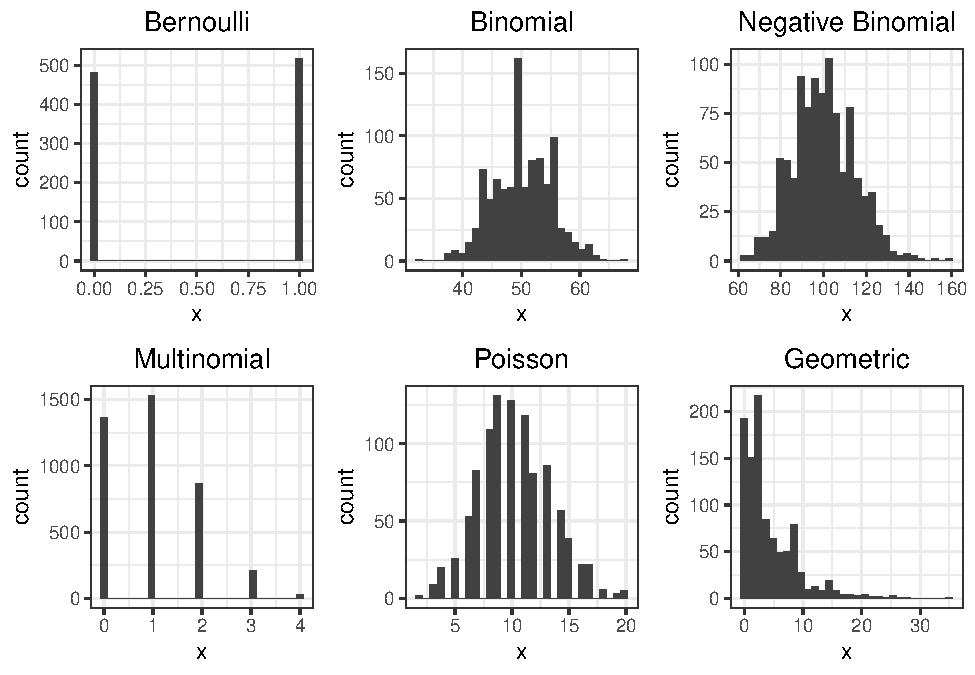
\includegraphics{People_Analytics_Lifecycle_files/figure-latex/discrete-dist-1} 

}

\caption{Discrete Probability Distributions}\label{fig:discrete-dist}
\end{figure}

\textbf{Continuous Probability Distributions}

\textbf{Continuous probability distributions}, also known as \textbf{Probability Density Functions (PDF)}, can be leveraged to model different types of interval and ratio variables. Some common continuous distributions include:

\begin{itemize}
\tightlist
\item
  \textbf{Normal (Gaussian)}: distribution characterized by a mean and standard deviation for which the mean, median, and mode are equal
\item
  \textbf{Uniform}: values of a random variable with equal probabilities of occurring
\item
  \textbf{Log-Normal}: normal distribution of log-transformed values
\item
  \textbf{Student's T}: similar to the normal distribution but with thicker tails (approaches normal as \(n\) increases)
\item
  \textbf{Chi-Square}: similar to the t distribution in that the shape approaches normal as \(n\) increases
\item
  \textbf{F}: developed to examine variances from random samples taken from two independent normal populations
\end{itemize}

A number of functions are available in R to simulate PDFs. While the precise shape of a distribution depends on the parameters, we will simulate and visualize these common PDFs to illustrate differences in the general shape of each. Let's first draw 1,000 random values from each distribution with a specified set of parameters:

\begin{Shaded}
\begin{Highlighting}[]
\CommentTok{\# Set seed for reproducible random distribution}
\FunctionTok{set.seed}\NormalTok{(}\DecValTok{1234}\NormalTok{)}

\CommentTok{\# Simulate normal distribution}
\NormalTok{normal\_dist }\OtherTok{\textless{}{-}} \FunctionTok{rnorm}\NormalTok{(}\DecValTok{1000}\NormalTok{, }\AttributeTok{mean =} \DecValTok{50}\NormalTok{, }\AttributeTok{sd =} \DecValTok{5}\NormalTok{)}

\CommentTok{\# Simulate log{-}normal distribution}
\NormalTok{lnormal\_dist }\OtherTok{\textless{}{-}} \FunctionTok{rlnorm}\NormalTok{(}\DecValTok{1000}\NormalTok{, }\AttributeTok{meanlog =} \DecValTok{0}\NormalTok{, }\AttributeTok{sdlog =} \DecValTok{1}\NormalTok{)}

\CommentTok{\# Simulate uniform distribution}
\NormalTok{uniform\_dist }\OtherTok{\textless{}{-}} \FunctionTok{runif}\NormalTok{(}\DecValTok{1000}\NormalTok{, }\AttributeTok{min =} \DecValTok{1}\NormalTok{, }\AttributeTok{max =} \DecValTok{100}\NormalTok{) }

\CommentTok{\# Simulate student\textquotesingle{}s t distribution}
\NormalTok{t\_dist }\OtherTok{\textless{}{-}} \FunctionTok{rt}\NormalTok{(}\DecValTok{1000}\NormalTok{, }\AttributeTok{df =} \DecValTok{5}\NormalTok{)}

\CommentTok{\# Simulate chi{-}square distribution}
\NormalTok{chisq\_dist }\OtherTok{\textless{}{-}} \FunctionTok{rchisq}\NormalTok{(}\DecValTok{1000}\NormalTok{, }\AttributeTok{df =} \DecValTok{5}\NormalTok{)}

\CommentTok{\# Simulate F distribution}
\NormalTok{f\_dist }\OtherTok{\textless{}{-}} \FunctionTok{rf}\NormalTok{(}\DecValTok{1000}\NormalTok{, }\AttributeTok{df1 =} \DecValTok{5}\NormalTok{, }\AttributeTok{df2 =} \DecValTok{200}\NormalTok{)}
\end{Highlighting}
\end{Shaded}

Next, we will visualize each distribution. Since these continuous distributions are probability \emph{density} functions, we will superimpose density plots over each:

\begin{Shaded}
\begin{Highlighting}[]
\CommentTok{\# Call UDF to build visualizations and store to objects}
\CommentTok{\# Note that as long as the arguments are in the order specified in the function (see our UDF definition above), the argument names do not need to be specified. To illustrate, we will drop the argument names from these function calls:}
\NormalTok{p\_normal }\OtherTok{\textless{}{-}} \FunctionTok{dist.viz}\NormalTok{(normal\_dist, }\StringTok{"continuous"}\NormalTok{, }\StringTok{"Normal"}\NormalTok{)}
\NormalTok{p\_lnormal }\OtherTok{\textless{}{-}} \FunctionTok{dist.viz}\NormalTok{(lnormal\_dist, }\StringTok{"continuous"}\NormalTok{, }\StringTok{"Log{-}Normal"}\NormalTok{)}
\NormalTok{p\_uniform }\OtherTok{\textless{}{-}} \FunctionTok{dist.viz}\NormalTok{(uniform\_dist, }\StringTok{"continuous"}\NormalTok{, }\StringTok{"Uniform"}\NormalTok{)}
\NormalTok{p\_t }\OtherTok{\textless{}{-}} \FunctionTok{dist.viz}\NormalTok{(t\_dist, }\StringTok{"continuous"}\NormalTok{, }\StringTok{"Student\textquotesingle{}s T"}\NormalTok{)}
\NormalTok{p\_chisq }\OtherTok{\textless{}{-}} \FunctionTok{dist.viz}\NormalTok{(chisq\_dist, }\StringTok{"continuous"}\NormalTok{, }\StringTok{"Chi{-}Square"}\NormalTok{)}
\NormalTok{p\_f }\OtherTok{\textless{}{-}} \FunctionTok{dist.viz}\NormalTok{(f\_dist, }\StringTok{"continuous"}\NormalTok{, }\StringTok{"F"}\NormalTok{)}

\CommentTok{\# Display distribution visualizations}
\NormalTok{ggpubr}\SpecialCharTok{::}\FunctionTok{ggarrange}\NormalTok{(p\_normal, p\_lnormal, p\_uniform, p\_t, p\_chisq, p\_f,}
          \AttributeTok{ncol =} \DecValTok{3}\NormalTok{, }\AttributeTok{nrow =} \DecValTok{2}\NormalTok{)}
\end{Highlighting}
\end{Shaded}

\begin{figure}

{\centering 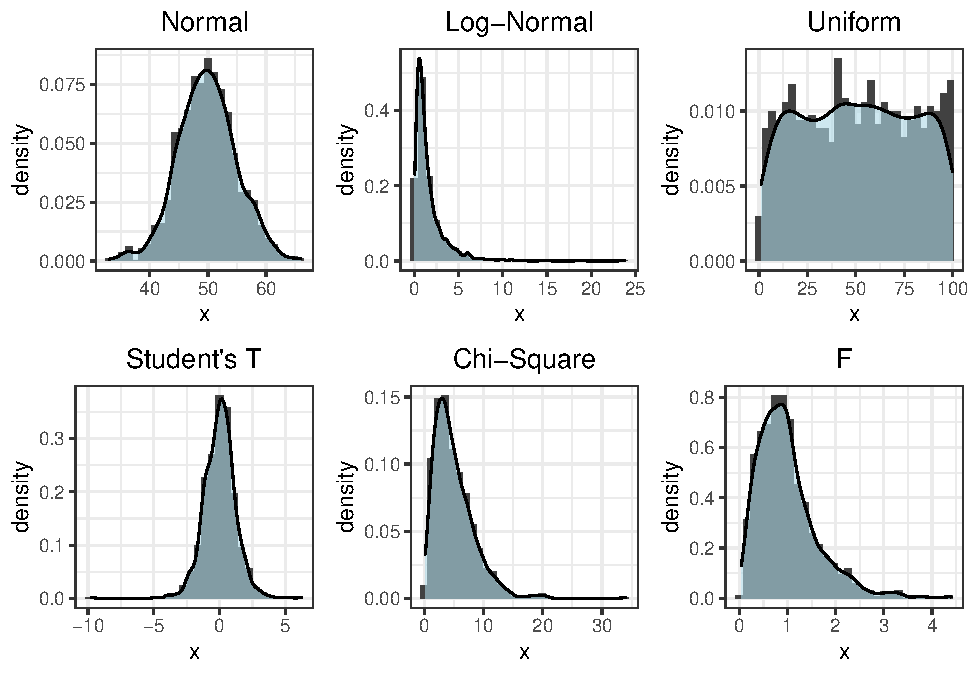
\includegraphics{People_Analytics_Lifecycle_files/figure-latex/continous-dist-1} 

}

\caption{Continuous Probability Distributions}\label{fig:continous-dist}
\end{figure}

The distribution of data is critically important in statistics. The accuracy of many statistical tests is based on assumptions rooted in underlying data distributions, and violating these assumptions can result in serious errors due to misaligned probability distributions. Though there are many more discrete and continuous probability distributions, we will leverage several of these common types to assess the likelihood of differences, effects, and associations in later chapters of this book.

\hypertarget{conditional-probability}{%
\subsection{Conditional Probability}\label{conditional-probability}}

\textbf{Conditional probability} reflects the probability conditioned on the occurrence of a previous event or outcome. For example, we may find that the proportion of heads is greater or less than \(\frac{1}{2}\) with a large number of fair coin flips when the coin is consistently heads up when flipped. The outcome is, therefore, conditioned on the fixed -- rather than random -- positioning of the coin when flipped.

Formally, \textbf{Bayes' Theorem (alternatively, Bayes' Rule)} states that for any two events A and B wherein the probability of A is not 0 (\(P(A) \neq 0\)):

\[ P(A \vert B) = \frac{P(B \vert A) P(A)}{P(B)}, \]

where:

\begin{itemize}
\tightlist
\item
  \(A\) = an event
\item
  \(B\) = another event
\item
  \(P(A|B)\) = conditional probability that event A occurs, given event B occurs (posterior)
\item
  \(P(B|A)\) = conditional probability that event B occurs, given event A occurs (likelihood)
\item
  \(P(B)\) = normalizing constant, constraining the probability distribution to sum to 1 (evidence)
\item
  \(P(A)\) = probability event A occurs before knowing if event B occurs (prior)
\end{itemize}

Bayes' Rule allows us to predict the outcome more accurately by conditioning the probability on known factors rather than assuming all events operate under the same conditions. Bayes' Rule is pervasive in people analytics, as the probability of outcomes can vary widely when conditioned on a person's age, tenure, education, job, perceptions, relationships, and many other factors. For example, if we consider a company with 100 terminations over a 12-month period and average headcount of 1,000, the probability of attrition not conditioned on any other factor is 10\%, or \(\frac{1}{10}\). Aside from trending this probability over time to identify if overall attrition is becoming more or less of a concern, this isn't too helpful at the company level. However, if we condition the probability of attrition on an event -- such as a recent manager exit -- and find that the probability of attrition among those whose manager has left in the last six months is 70\%, or \(\frac{7}{10}\), this is far more actionable (and concerning).

The \textbf{Monty Hall Problem} is an excellent example of how our intuition is often at odds with the laws of conditional probability.

In the classic game show, Let's Make a Deal, Monty Hall asks contestants to choose one of three closed doors. Behind one door is a prize while the other two doors contain nothing. After the contestant selects a door, Monty opens one of the other two doors which does not contain a prize. At this point, there are two closed doors: the door the contestant selected and another for which the content remains unknown. All that is known at this point is that the prize is behind one of the two closed doors.

It is at this juncture that Monty introduces a twist by asking if the contestant would like to switch doors. Most assume that the two closed doors have an equal (50/50) chance of containing the prize, because we generally think of probabilities as independent, random events. However, this is incorrect. Contestants who switch from their original selection have a 66\% chance (rather than 50\%) of winning. This may be counterintuitive, because the brain wants to reduce the problem to a simple coin flip. There is a major difference between the Monty Hall problem and a coin flip; for two outcomes to have the same probability, randomness and independence are required. In the case of the Monty Hall problem, neither assumption is satisfied.

When all three doors are closed, each has the same probability of being selected. The probability of choosing the door with a prize is .33. Monty's knowledge of the door containing the prize does not impact the probability of selecting the winning door. This is because the choice is completely random given we have no information that would increase the probability of a door containing the prize. The process is no longer random when Monty uses his insider knowledge about the prize's location and opens a door he knows does not contain the prize. The probabilities change. Since Monty will never show the door containing the prize, he is careful to always open a door that has nothing behind it. If he was not constrained by the requirement to not reveal the prize's location and instead chose to open one of the remaining doors at random, the probabilities would be equal (and he may end up opening the door that contains the prize).

Seeing is believing, so let's prove this with a simulation in R:

\begin{Shaded}
\begin{Highlighting}[]
\CommentTok{\# Set seed for reproducible simulations}
\FunctionTok{set.seed}\NormalTok{(}\DecValTok{12345}\NormalTok{)}

\CommentTok{\# Set number of simulations}
\NormalTok{trials }\OtherTok{=} \DecValTok{10000}

\CommentTok{\# Store switch/keep decisions}
\NormalTok{decisions }\OtherTok{=} \FunctionTok{c}\NormalTok{(}\StringTok{"switch"}\NormalTok{, }\StringTok{"keep"}\NormalTok{)}

\CommentTok{\# Store integer for each door}
\NormalTok{doors }\OtherTok{=} \DecValTok{1}\SpecialCharTok{:}\DecValTok{3}

\CommentTok{\# Initialize empty data frame for results}
\NormalTok{results }\OtherTok{=} \ConstantTok{NULL}

\ControlFlowTok{for}\NormalTok{ (n }\ControlFlowTok{in} \DecValTok{1}\SpecialCharTok{:}\NormalTok{trials)\{}
  
  \ControlFlowTok{for}\NormalTok{ (decision }\ControlFlowTok{in}\NormalTok{ decisions)\{}
    
    \CommentTok{\# Select correct door}
\NormalTok{    correct\_door }\OtherTok{\textless{}{-}} \FunctionTok{sample}\NormalTok{(doors, }\DecValTok{1}\NormalTok{, }\AttributeTok{replace =}\NormalTok{ T)}

    \CommentTok{\# Contestant chooses a door at random}
\NormalTok{    selected\_door }\OtherTok{\textless{}{-}} \FunctionTok{sample}\NormalTok{(doors, }\DecValTok{1}\NormalTok{, }\AttributeTok{replace =}\NormalTok{ T)}
  
    \CommentTok{\# Open door that was neither selected by the contestant nor contains the prize}
    \CommentTok{\# Choose one door to open if multiple remain without the prize (i.e., the contestant didn\textquotesingle{}t initially select the door containing the prize)}
\NormalTok{    remaining\_doors }\OtherTok{\textless{}{-}} \FunctionTok{which}\NormalTok{(}\SpecialCharTok{!}\NormalTok{doors }\SpecialCharTok{==}\NormalTok{ correct\_door }\SpecialCharTok{\&} \SpecialCharTok{!}\NormalTok{doors }\SpecialCharTok{==}\NormalTok{ selected\_door)}
\NormalTok{    open\_door }\OtherTok{\textless{}{-}} \FunctionTok{sample}\NormalTok{(remaining\_doors, }\DecValTok{1}\NormalTok{, }\AttributeTok{replace =}\NormalTok{ T) }
  
    \CommentTok{\# Contestant makes decision to switch doors or keep with the originally selected door}
\NormalTok{    selected\_door }\OtherTok{\textless{}{-}} \FunctionTok{ifelse}\NormalTok{(decision }\SpecialCharTok{==} \StringTok{"switch"}\NormalTok{, }\FunctionTok{which}\NormalTok{(}\SpecialCharTok{!}\NormalTok{doors }\SpecialCharTok{==}\NormalTok{ selected\_door }\SpecialCharTok{\&} \SpecialCharTok{!}\NormalTok{doors }\SpecialCharTok{==}\NormalTok{ open\_door), selected\_door)}
    
    \CommentTok{\# Store results in data frame}
\NormalTok{    results }\OtherTok{\textless{}{-}} \FunctionTok{rbind}\NormalTok{(results, }\FunctionTok{cbind.data.frame}\NormalTok{(}
                     \AttributeTok{trial =}\NormalTok{ n,}
                     \AttributeTok{decision =}\NormalTok{ decision,}
                     \AttributeTok{result =} \FunctionTok{ifelse}\NormalTok{(correct\_door }\SpecialCharTok{==}\NormalTok{ selected\_door, }\StringTok{"win"}\NormalTok{, }\StringTok{"lose"}\NormalTok{)))}
\NormalTok{  \}}
\NormalTok{\}}

\CommentTok{\# Calculate percentage difference in wins for switch vs. keep decisions}
\NormalTok{switch\_wins }\OtherTok{\textless{}{-}} \FunctionTok{nrow}\NormalTok{(results[results}\SpecialCharTok{$}\NormalTok{decision }\SpecialCharTok{==} \StringTok{"switch"} \SpecialCharTok{\&}\NormalTok{ results}\SpecialCharTok{$}\NormalTok{result }\SpecialCharTok{==} \StringTok{"win"}\NormalTok{, ]) }\SpecialCharTok{/} \FunctionTok{nrow}\NormalTok{(results) }\SpecialCharTok{*} \DecValTok{100}
\NormalTok{keep\_wins }\OtherTok{\textless{}{-}} \FunctionTok{nrow}\NormalTok{(results[results}\SpecialCharTok{$}\NormalTok{decision }\SpecialCharTok{==} \StringTok{"keep"} \SpecialCharTok{\&}\NormalTok{ results}\SpecialCharTok{$}\NormalTok{result }\SpecialCharTok{==} \StringTok{"win"}\NormalTok{, ]) }\SpecialCharTok{/} \FunctionTok{nrow}\NormalTok{(results) }\SpecialCharTok{*} \DecValTok{100}
\FunctionTok{round}\NormalTok{((switch\_wins }\SpecialCharTok{{-}}\NormalTok{ keep\_wins) }\SpecialCharTok{/}\NormalTok{ keep\_wins }\SpecialCharTok{*} \DecValTok{100}\NormalTok{, }\DecValTok{0}\NormalTok{)}
\end{Highlighting}
\end{Shaded}

\begin{verbatim}
## [1] 45
\end{verbatim}

As we can see, wins occur nearly 50\% more often when contestants switch doors. This exercise hopefully demonstrates the importance of conditional probability and statistical assumptions like randomness. Also, if ever you find yourself playing Let's Make a Deal, switch doors.

\hypertarget{central-limit-theorem}{%
\section{Central Limit Theorem}\label{central-limit-theorem}}

The \textbf{Central Limit Theorem (CLT)} is a mainstay of statistics and probability and fundamental to understanding the mechanics of statistical inference. The CLT was initially coined by a French-born mathematician named Abraham De Moivre in the 1700s.

The CLT states that given a sufficiently large sample size, the average of independent random variables tends to follow a normal (or Gaussian) distribution as the number of samples increases. The distribution of sample means approaches a normal distribution regardless of the shape of the population distribution from which the samples are drawn. This is important because the normal distribution has properties that can be used to test the likelihood that an observed value, difference, or relationship in a sample is also present in the population.

\begin{figure}

{\centering 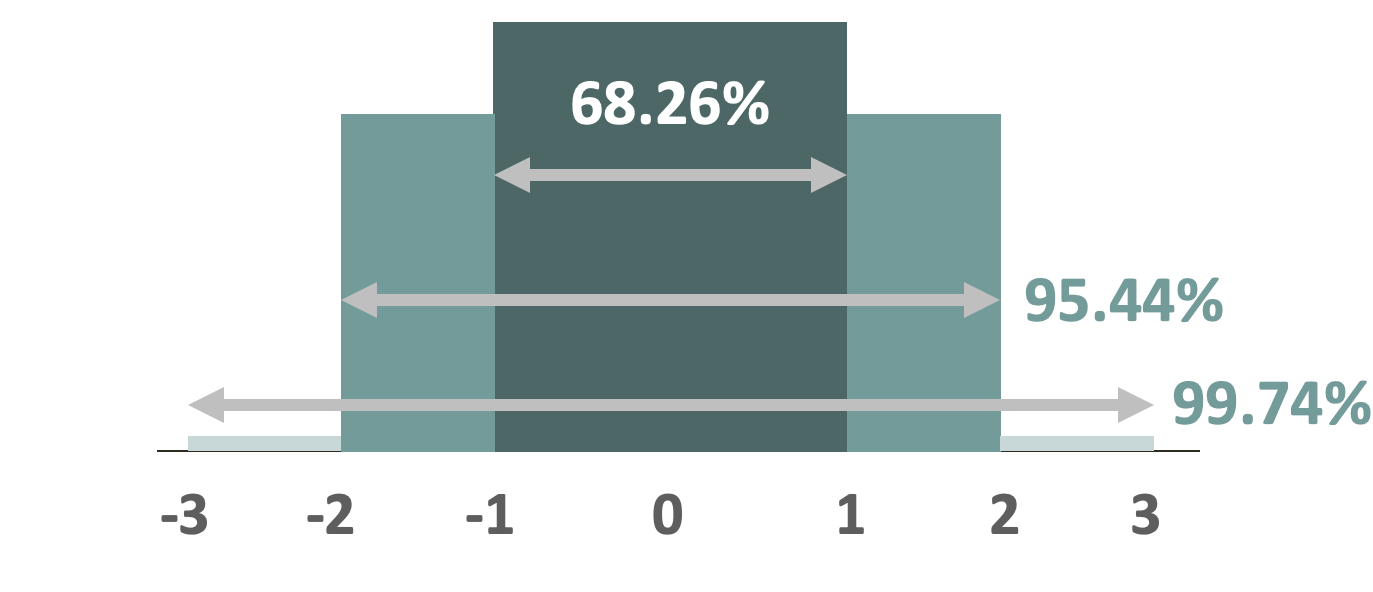
\includegraphics[width=0.75\linewidth]{/Users/craig.starbuck/Library/Mobile Documents/com~apple~CloudDocs/Documents/People Analytics Book/GitHub/peopleanalytics_lifecycle_book/graphics/normal_distribution} 

}

\caption{The Empirical Rule}\label{fig:emp-rule}
\end{figure}

Let's begin with an intuitive example of CLT. Imagine that we have a reliable way to measure how fun a population is on a 100-point scale, where 100 indicates maximum fun (life of the party) and 1 indicates maximum boringness. Consider that a small statistics conference is in progress at a nearby convention center, and there are 40 statisticians in attendance. In a separate room at the same convention center, there is also a group of 40 random people (non-statisticians) who are gathered to discuss some less interesting topic. Our job is to walk into one of the rooms and determine -- based on the ``fun'' factor alone -- whether we have entered the statistics conference or the other, less interesting gathering of non-statisticians.

Instinctively, we already know the statisticians will be more fun than the other group. However, let's assume we need the mean fun score and standard deviation of these two groups for this example. The group of statisticians have, on average, a fun score of 85 with a standard deviation of 2, while the group of non-statisticians are a bit less fun with a mean score of 65 and a standard deviation of 4. With a known population mean and standard deviation, the standard error (the standard deviation of the sample means) provides the ability to calculate the probability that the sample (the room of 40 people) belongs to the population of interest (fellow statisticians).

Herein lies the beauty of the CLT: roughly 68 percent of sample means will lie within one standard error of the population mean, roughly 95 percent within two standard errors of the population mean, and roughly 99 percent within three standard errors of the population mean. Therefore, any room whose members have an average fun score that is not within two standard errors of the population mean (between 81 and 89 for our statisticians) is statistically unlikely to be the group of statisticians for which we are searching. This is because in less than 5 in 100 cases could we randomly draw a `reasonably sized' sample of statisticians with average funness so extremely different from the population average.

Because small samples lend to anomalies, we could -- by chance -- select a single person who happens to fall in the tails (extremely boring or extremely fun); however, as the sample size increases, it becomes more and more likely that the observed average reflects the average of the larger population. It would be virtually impossible (in less than 1 in 100 cases) to draw a random sample of statisticians from the population with average funness that is not within three standard errors of the population mean (between 79 and 91). Therefore, if we find that the room of people have an average fun score of 75, we will likely have far more fun in the other room!

Let's now see the CLT in action by simulating a random uniform population distribution from which we can draw random samples. Remember, the shape of the population distribution does not matter; we could simulate an Exponential, Gamma, Poisson, Binomial, or other distribution and observe the same behavior.

\begin{Shaded}
\begin{Highlighting}[]
\CommentTok{\# Set seed for reproducible random distribution}
\FunctionTok{set.seed}\NormalTok{(}\DecValTok{1234}\NormalTok{)}

\CommentTok{\# Generate uniform population distribution with 1000 values ranging from 1 to 100}
\NormalTok{rand.unif }\OtherTok{\textless{}{-}} \FunctionTok{runif}\NormalTok{(}\DecValTok{1000}\NormalTok{, }\AttributeTok{min =} \DecValTok{1}\NormalTok{, }\AttributeTok{max =} \DecValTok{100}\NormalTok{)}
\end{Highlighting}
\end{Shaded}

\begin{Shaded}
\begin{Highlighting}[]
\CommentTok{\# Calculate population mean}
\FunctionTok{mean}\NormalTok{(rand.unif)}
\end{Highlighting}
\end{Shaded}

\begin{verbatim}
## [1] 51.22007
\end{verbatim}

\begin{Shaded}
\begin{Highlighting}[]
\CommentTok{\# Calculate population variance}
\NormalTok{N }\OtherTok{=} \FunctionTok{length}\NormalTok{(rand.unif)}
\FunctionTok{var}\NormalTok{(rand.unif) }\SpecialCharTok{*}\NormalTok{ (N }\SpecialCharTok{{-}} \DecValTok{1}\NormalTok{) }\SpecialCharTok{/}\NormalTok{ N}
\end{Highlighting}
\end{Shaded}

\begin{verbatim}
## [1] 830.3155
\end{verbatim}

\begin{Shaded}
\begin{Highlighting}[]
\CommentTok{\# Produce histogram to visualize population distribution}
\NormalTok{ggplot2}\SpecialCharTok{::}\FunctionTok{ggplot}\NormalTok{() }\SpecialCharTok{+} 
\NormalTok{ggplot2}\SpecialCharTok{::}\FunctionTok{aes}\NormalTok{(rand.unif) }\SpecialCharTok{+} 
\NormalTok{ggplot2}\SpecialCharTok{::}\FunctionTok{labs}\NormalTok{(}\AttributeTok{x =} \StringTok{"x"}\NormalTok{, }\AttributeTok{y =} \StringTok{"Density"}\NormalTok{) }\SpecialCharTok{+} 
\NormalTok{ggplot2}\SpecialCharTok{::}\FunctionTok{geom\_histogram}\NormalTok{(}\FunctionTok{aes}\NormalTok{(}\AttributeTok{y =}\NormalTok{ ..density..), }\AttributeTok{fill =} \StringTok{"\#414141"}\NormalTok{) }\SpecialCharTok{+}
\NormalTok{ggplot2}\SpecialCharTok{::}\FunctionTok{geom\_density}\NormalTok{(}\AttributeTok{fill =} \StringTok{"\#ADD8E6"}\NormalTok{, }\AttributeTok{alpha =} \FloatTok{0.6}\NormalTok{) }\SpecialCharTok{+}
\NormalTok{ggplot2}\SpecialCharTok{::}\FunctionTok{theme\_bw}\NormalTok{()}
\end{Highlighting}
\end{Shaded}

\begin{figure}

{\centering 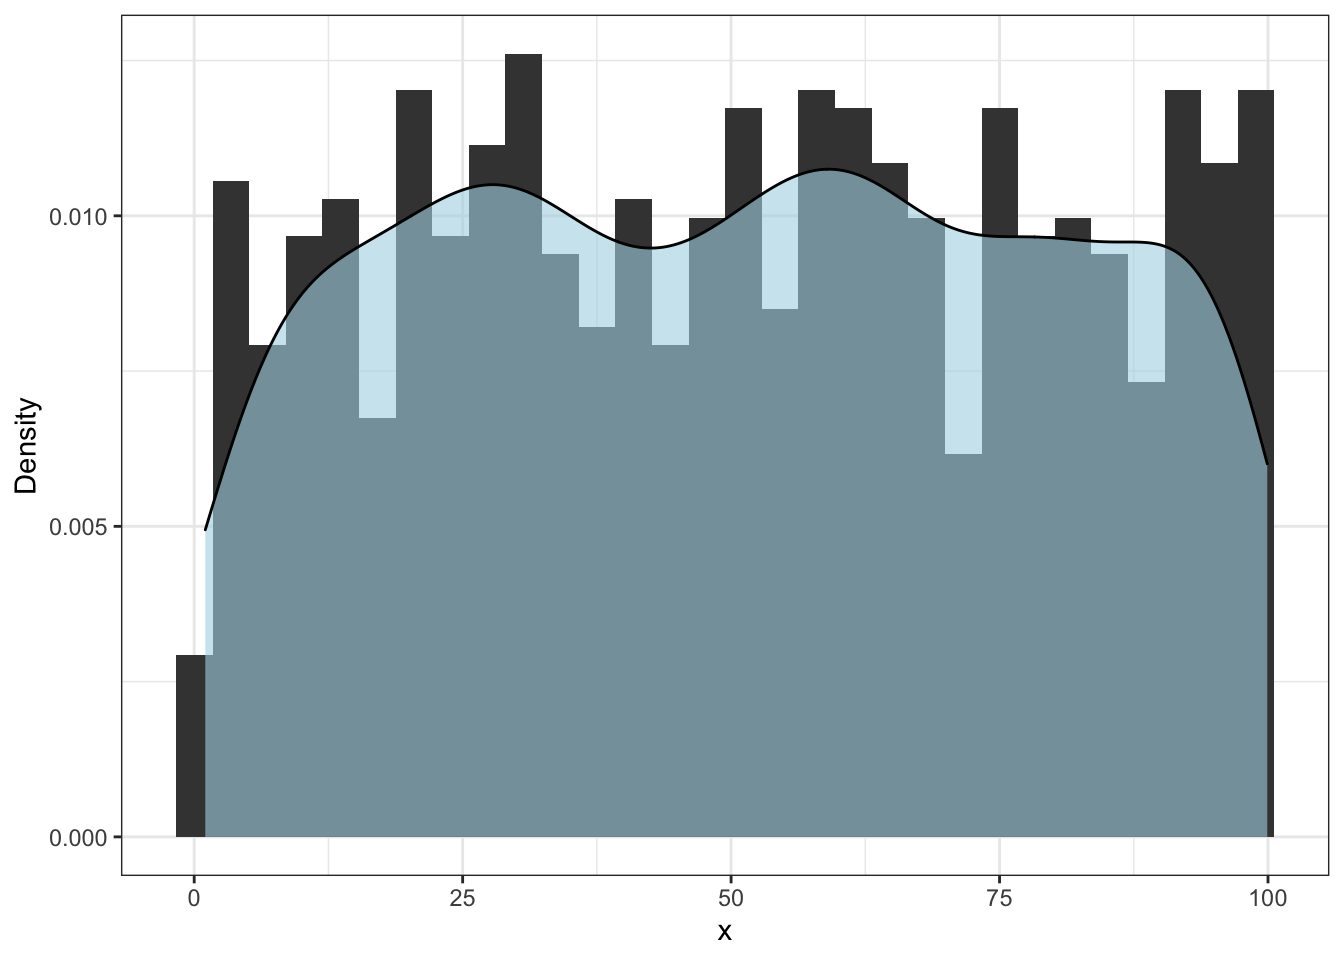
\includegraphics{People_Analytics_Lifecycle_files/figure-latex/unnamed-chunk-115-1} 

}

\caption{Uniform Population Distribution (N = 1000)}\label{fig:unnamed-chunk-115}
\end{figure}

As expected, these randomly generated data are uniformly distributed. Next, we will draw 100 random samples of various sizes and plot the average of each.

\begin{Shaded}
\begin{Highlighting}[]
\CommentTok{\# Define number of samples to draw from population distribution}
\NormalTok{samples }\OtherTok{\textless{}{-}} \DecValTok{10000}

\CommentTok{\# Populate vector with sample sizes}
\NormalTok{sample\_n }\OtherTok{\textless{}{-}} \FunctionTok{c}\NormalTok{(}\DecValTok{1}\SpecialCharTok{:}\DecValTok{5}\NormalTok{,}\DecValTok{10}\NormalTok{,}\DecValTok{25}\NormalTok{,}\DecValTok{50}\NormalTok{)}

\CommentTok{\# Initialize empty data frame to hold sample means}
\NormalTok{sample\_means }\OtherTok{=} \ConstantTok{NULL}

\CommentTok{\# Set seed for reproducible random samples}
\FunctionTok{set.seed}\NormalTok{(}\DecValTok{456}\NormalTok{)}

\CommentTok{\# For each n, draw random samples}
\ControlFlowTok{for}\NormalTok{ (n }\ControlFlowTok{in}\NormalTok{ sample\_n) \{}
  
  \ControlFlowTok{for}\NormalTok{ (draw }\ControlFlowTok{in} \DecValTok{1}\SpecialCharTok{:}\NormalTok{samples) \{}
    
      \CommentTok{\# Store sample means in data frame}
\NormalTok{      sample\_means }\OtherTok{\textless{}{-}} \FunctionTok{rbind}\NormalTok{(sample\_means, }\FunctionTok{cbind.data.frame}\NormalTok{(}
                            \AttributeTok{n =}\NormalTok{ n, }
                            \AttributeTok{x\_bar =} \FunctionTok{mean}\NormalTok{(}\FunctionTok{sample}\NormalTok{(rand.unif, n, }\AttributeTok{replace =} \ConstantTok{TRUE}\NormalTok{, }\AttributeTok{prob =} \ConstantTok{NULL}\NormalTok{))))}
\NormalTok{  \}}
\NormalTok{\}}

\CommentTok{\# Produce histograms to visualize distributions of sample means, grouped by n{-}count}
\NormalTok{sample\_means }\SpecialCharTok{\%\textgreater{}\%}\NormalTok{ ggplot2}\SpecialCharTok{::}\FunctionTok{ggplot}\NormalTok{() }\SpecialCharTok{+} 
\NormalTok{                 ggplot2}\SpecialCharTok{::}\FunctionTok{aes}\NormalTok{(}\AttributeTok{x =}\NormalTok{ x\_bar, }\AttributeTok{fill =}\NormalTok{ n) }\SpecialCharTok{+} 
\NormalTok{                 ggplot2}\SpecialCharTok{::}\FunctionTok{labs}\NormalTok{(}\AttributeTok{x =} \StringTok{"x{-}bar"}\NormalTok{, }\AttributeTok{y =} \StringTok{"Density"}\NormalTok{) }\SpecialCharTok{+} 
\NormalTok{                 ggplot2}\SpecialCharTok{::}\FunctionTok{geom\_histogram}\NormalTok{(}\FunctionTok{aes}\NormalTok{(}\AttributeTok{y =}\NormalTok{ ..density..), }\AttributeTok{fill =} \StringTok{"\#414141"}\NormalTok{) }\SpecialCharTok{+}
\NormalTok{                 ggplot2}\SpecialCharTok{::}\FunctionTok{geom\_density}\NormalTok{(}\AttributeTok{fill =} \StringTok{"\#ADD8E6"}\NormalTok{, }\AttributeTok{alpha =} \FloatTok{0.6}\NormalTok{) }\SpecialCharTok{+}
\NormalTok{                 ggplot2}\SpecialCharTok{::}\FunctionTok{theme\_bw}\NormalTok{() }\SpecialCharTok{+}
\NormalTok{                 ggplot2}\SpecialCharTok{::}\FunctionTok{facet\_wrap}\NormalTok{(}\SpecialCharTok{\textasciitilde{}}\NormalTok{n)}
\end{Highlighting}
\end{Shaded}

\begin{figure}

{\centering 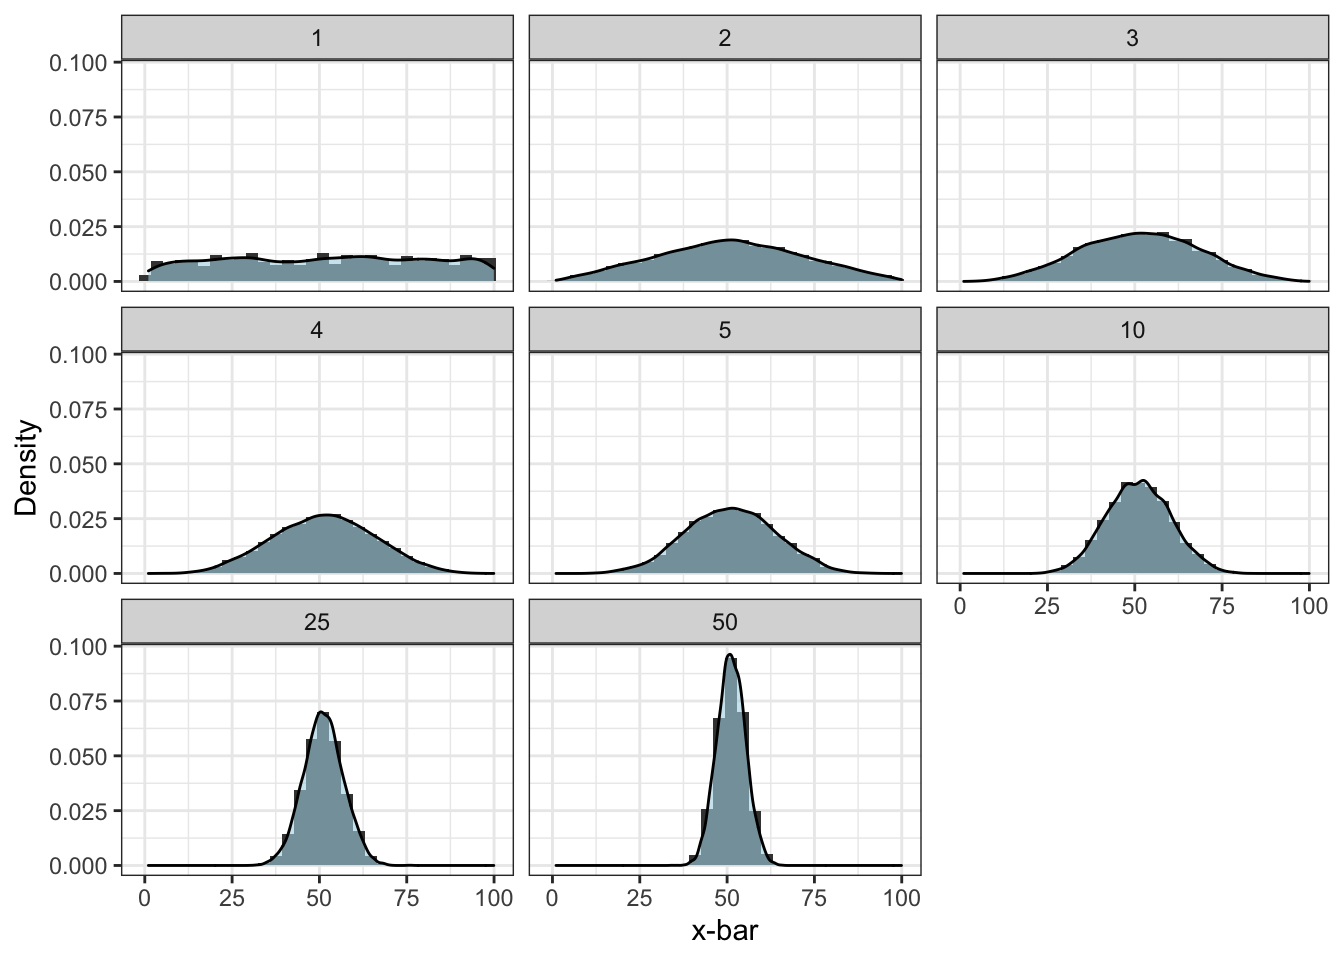
\includegraphics{People_Analytics_Lifecycle_files/figure-latex/unnamed-chunk-116-1} 

}

\caption{Distribution of 10,000 Sample Means of Varied Size}\label{fig:unnamed-chunk-116}
\end{figure}

Per the CLT, we can see that as n increases, the sample means become more normally distributed.

\hypertarget{confidence-intervals}{%
\section{Confidence Intervals}\label{confidence-intervals}}

A \textbf{Confidence Interval (CI)} is a range of values that likely contains the value of an unknown population parameter. These unknown population parameters are often \(\mu\) or \(\sigma\), though we will also leverage CIs in later chapters for regression coefficients, proportions, rates, and differences.

If we draw random samples from a population, we can compute a CI for each sample. Building on the CLT, for a given confidence level (usually 95\%, though 99\% or 90\% are sometimes used), the specified percent of sample intervals is expected to include the estimated population parameter. For example, for a 95\% CI we would expect 19 in every 20 (or 95 in every 100) intervals across the samples to include the true population parameter. This is illustrated in Figure \ref{fig:conf-int}:

\begin{figure}

{\centering 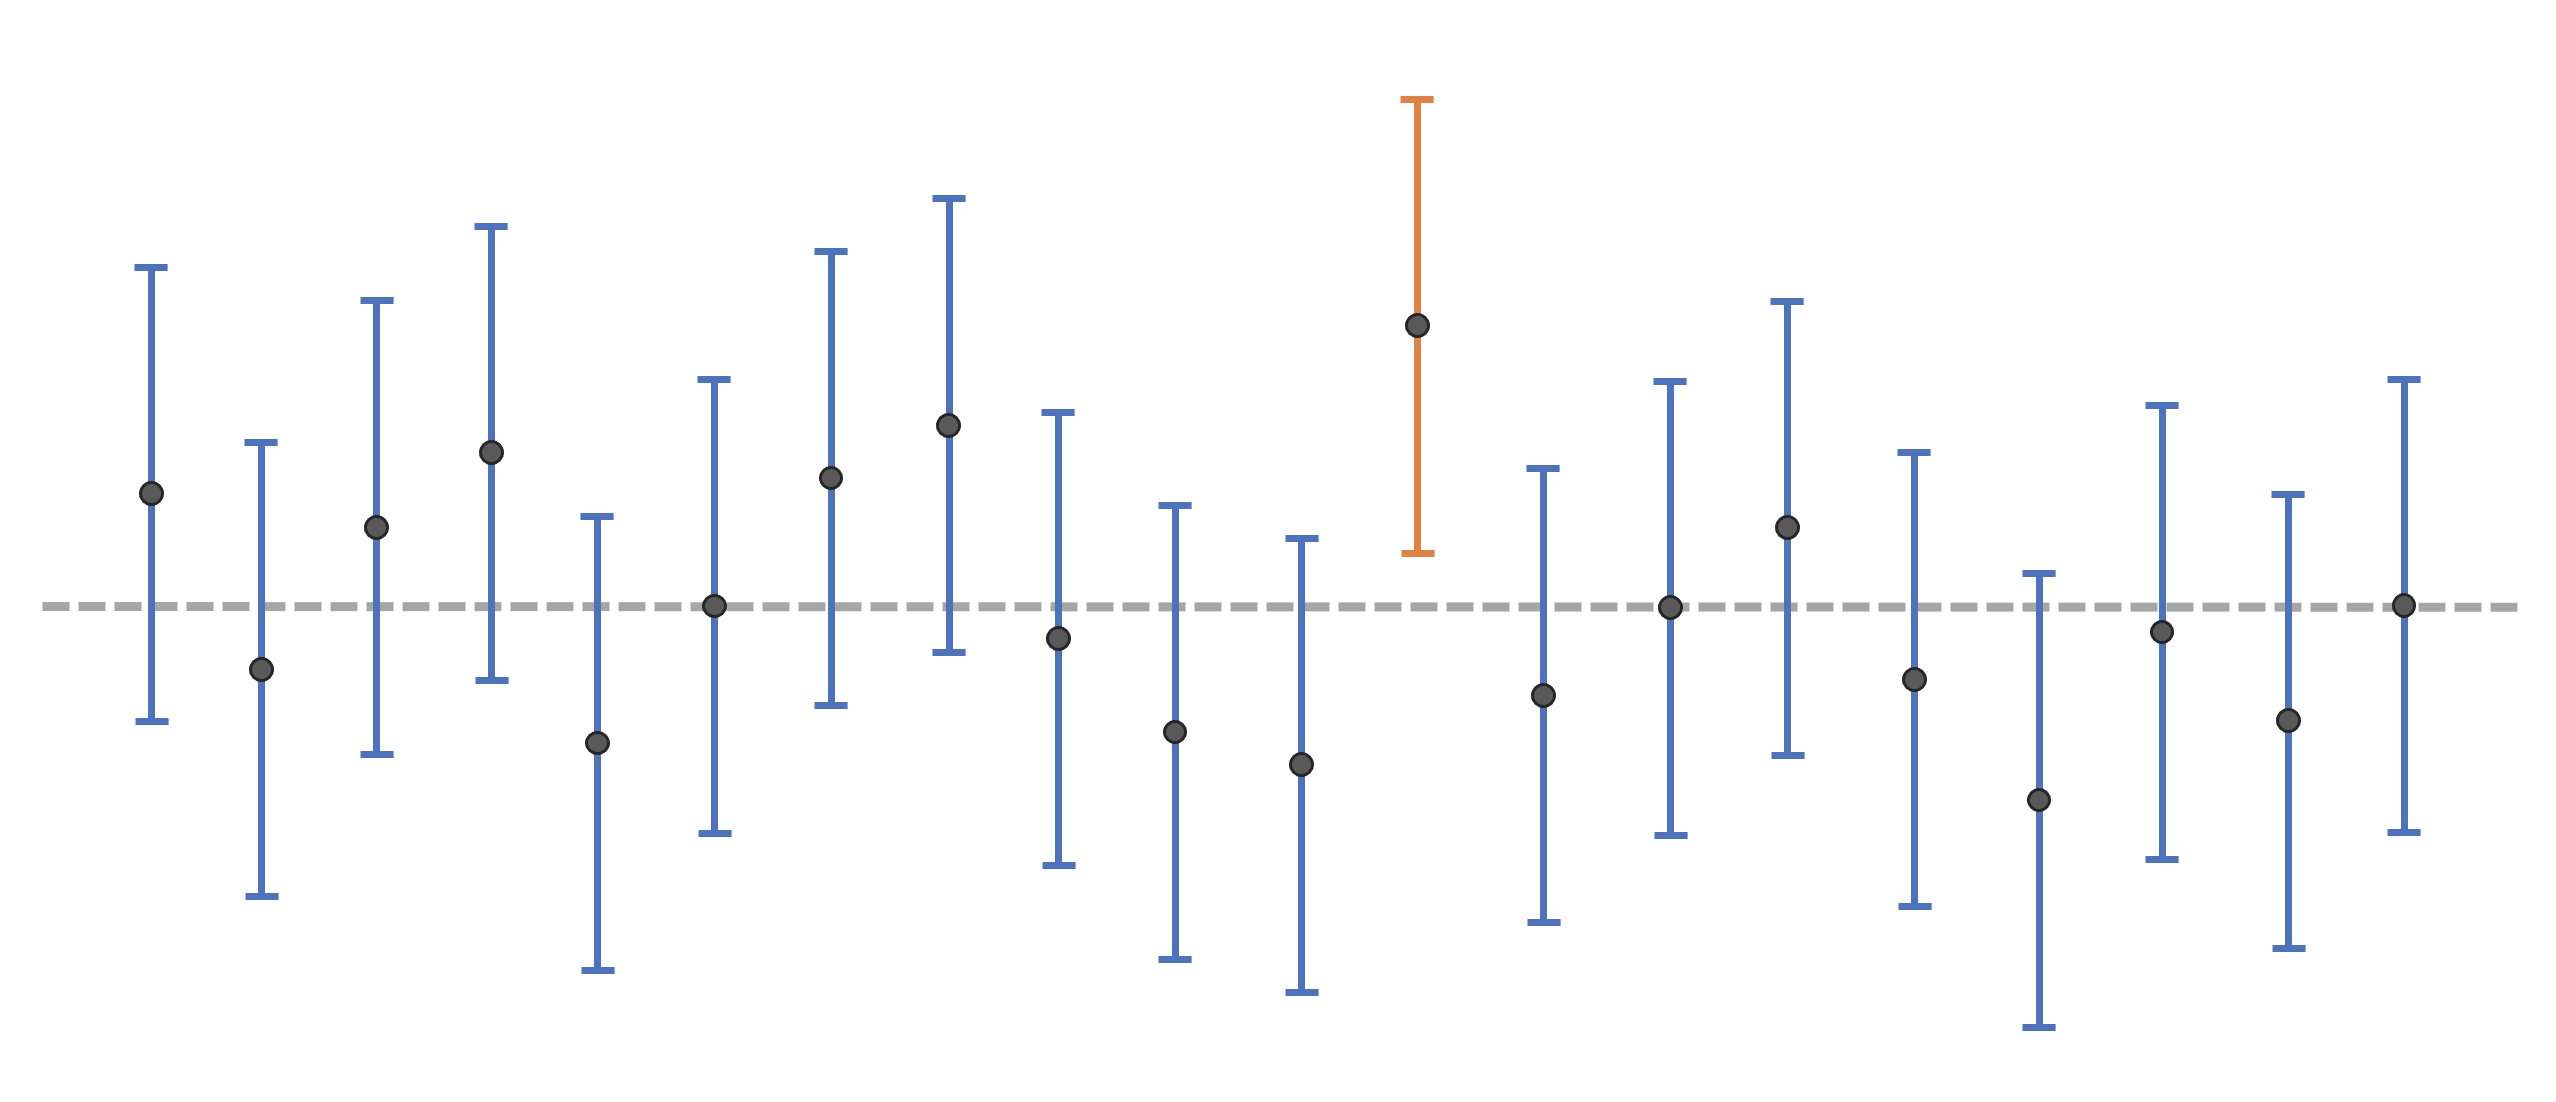
\includegraphics[width=0.75\linewidth]{/Users/craig.starbuck/Library/Mobile Documents/com~apple~CloudDocs/Documents/People Analytics Book/GitHub/peopleanalytics_lifecycle_book/graphics/confidence_intervals} 

}

\caption{Intervals for 95 Percent Confidence Level}\label{fig:conf-int}
\end{figure}

It is important to note that CIs should not be applied to the distribution of sample values; CIs relate to \emph{population parameters}. A common misinterpretation of a CI is that it represents an interval within which a certain percent of sample values exists, and this is inaccurate. Because this misinterpretation is so prevalent, there is a good chance you will be tested on your understanding of CIs when applying to positions involving statistical analyses!

A related concept that is fundamental to estimating CIs is the \textbf{standard error (SE)}, which is the standard deviation of sample means. While the standard deviation is a measure of variability for a random variable, the variability captured by the SE reflects how well a sample represents the population. Since sample statistics will approach the actual population parameters as the size of the sample increases, the SE and sample size are inversely related; that is, the SE decreases as the sample size increases. The SE is defined by:

\[ SE = \frac{\sigma}{\sqrt{n}} \]

Since the CLT is fundamental to inferential statistics, let's validate that our simulated distribution of sample means adheres to the properties of normally distributed data per the Empirical Rule:

\begin{Shaded}
\begin{Highlighting}[]
\CommentTok{\# Store sample means with n = 50}
\NormalTok{x\_bars }\OtherTok{\textless{}{-}}\NormalTok{ sample\_means[sample\_means}\SpecialCharTok{$}\NormalTok{n }\SpecialCharTok{==} \DecValTok{50}\NormalTok{, }\StringTok{"x\_bar"}\NormalTok{]}

\CommentTok{\# Store sample size}
\NormalTok{n }\OtherTok{\textless{}{-}} \FunctionTok{length}\NormalTok{(x\_bars)}

\CommentTok{\# Calculate percent of sample means within +/{-} 2 SEs}
\FunctionTok{length}\NormalTok{(}\FunctionTok{subset}\NormalTok{(x\_bars, x\_bars }\SpecialCharTok{\textless{}} \FunctionTok{mean}\NormalTok{(x\_bars) }\SpecialCharTok{+} \DecValTok{2} \SpecialCharTok{*} \FunctionTok{sd}\NormalTok{(x\_bars) }\SpecialCharTok{\&}\NormalTok{ x\_bars }\SpecialCharTok{\textgreater{}} \FunctionTok{mean}\NormalTok{(x\_bars) }\SpecialCharTok{{-}} \DecValTok{2} \SpecialCharTok{*} \FunctionTok{sd}\NormalTok{(x\_bars))) }\SpecialCharTok{/}\NormalTok{ n }\SpecialCharTok{*} \DecValTok{100}
\end{Highlighting}
\end{Shaded}

\begin{verbatim}
## [1] 95.35
\end{verbatim}

95\% of sample means are within 2 SEs, which is what we expect per the characteristics of the normal distribution.

\begin{Shaded}
\begin{Highlighting}[]
\CommentTok{\# Calculate percent of sample means within +/{-} 3 SEs}
\FunctionTok{length}\NormalTok{(}\FunctionTok{subset}\NormalTok{(x\_bars, x\_bars }\SpecialCharTok{\textless{}} \FunctionTok{mean}\NormalTok{(x\_bars) }\SpecialCharTok{+} \DecValTok{3} \SpecialCharTok{*} \FunctionTok{sd}\NormalTok{(x\_bars) }\SpecialCharTok{\&}\NormalTok{ x\_bars }\SpecialCharTok{\textgreater{}} \FunctionTok{mean}\NormalTok{(x\_bars) }\SpecialCharTok{{-}} \DecValTok{3} \SpecialCharTok{*} \FunctionTok{sd}\NormalTok{(x\_bars))) }\SpecialCharTok{/}\NormalTok{ n }\SpecialCharTok{*} \DecValTok{100}
\end{Highlighting}
\end{Shaded}

\begin{verbatim}
## [1] 99.79
\end{verbatim}

Nearly all of the sample means are within 3 SEs, indicating that it would be highly unlikely -- nearly impossible even -- to observe a sample mean `from the same population' that falls outside this interval.

Now, let's illustrate the relationship between CIs and standard errors using sample data from our uniform population distribution. In our example, both \(\mu\) and \(\sigma\) are known and our sample size \(n\) is at least 30; therefore, we can use a \textbf{Z-Test} to calculate the 95\% CI. A \(z\) score of 1.96 corresponds to the 95\% CI for a two-tailed distribution; that is, we are looking for significantly different values in either the larger or smaller direction. The 95\% CI represents the range of values we would expect to include \(\mu\) in at least 95 of 100 random samples taken from the population.

The CI in this case is defined by:

\[ CI = \bar{x} \pm z_{\alpha/_2} \frac{\sigma}{\sqrt{n}} \]

Let's randomly take \(n\) = 100 from the population, and compute sample statistics to estimate the 95\% CI:

\begin{Shaded}
\begin{Highlighting}[]
\CommentTok{\# Set seed for reproducible random samples}
\FunctionTok{set.seed}\NormalTok{(}\DecValTok{456}\NormalTok{)}

\CommentTok{\# Sample 100 values from uniform population distribution}
\NormalTok{x }\OtherTok{\textless{}{-}} \FunctionTok{sample}\NormalTok{(rand.unif, }\DecValTok{100}\NormalTok{, }\AttributeTok{replace =} \ConstantTok{TRUE}\NormalTok{, }\AttributeTok{prob =} \ConstantTok{NULL}\NormalTok{)}

\CommentTok{\# Calculate 95\% CI}
\NormalTok{ci95\_lower\_bound }\OtherTok{\textless{}{-}} \FunctionTok{mean}\NormalTok{(x) }\SpecialCharTok{{-}} \FloatTok{1.96} \SpecialCharTok{*}\NormalTok{ (}\FunctionTok{sd}\NormalTok{(x) }\SpecialCharTok{/} \FunctionTok{sqrt}\NormalTok{(}\DecValTok{100}\NormalTok{))}
\NormalTok{ci95\_upper\_bound }\OtherTok{\textless{}{-}} \FunctionTok{mean}\NormalTok{(x) }\SpecialCharTok{+} \FloatTok{1.96} \SpecialCharTok{*}\NormalTok{ (}\FunctionTok{sd}\NormalTok{(x) }\SpecialCharTok{/} \FunctionTok{sqrt}\NormalTok{(}\DecValTok{100}\NormalTok{))}
\end{Highlighting}
\end{Shaded}

\begin{Shaded}
\begin{Highlighting}[]
\CommentTok{\# Print lower bound for 95\% CI}
\NormalTok{ci95\_lower\_bound}
\end{Highlighting}
\end{Shaded}

\begin{verbatim}
## [1] 47.90733
\end{verbatim}

\begin{Shaded}
\begin{Highlighting}[]
\CommentTok{\# Print upper bound for 95\% CI}
\NormalTok{ci95\_upper\_bound}
\end{Highlighting}
\end{Shaded}

\begin{verbatim}
## [1] 58.98773
\end{verbatim}

Our known \(\mu\) is 51.2, which is covered by our 95\% CI (47.9 - 59.0). Per the CLT, in less than 5\% of cases would we expect to draw a random sample from the population that results in a 95\% CI which does not include \(\mu\). Note that our CI narrows with larger samples since our confidence that the range includes \(\mu\) increases with more data.

Next, let's look at a 99\% CI. We will enter 2.576 for \(z\):

\begin{Shaded}
\begin{Highlighting}[]
\CommentTok{\# Calculate 99\% CI}
\NormalTok{ci99\_lower\_bound }\OtherTok{\textless{}{-}} \FunctionTok{mean}\NormalTok{(x) }\SpecialCharTok{{-}} \FloatTok{2.576} \SpecialCharTok{*}\NormalTok{ (}\FunctionTok{sd}\NormalTok{(x) }\SpecialCharTok{/} \FunctionTok{sqrt}\NormalTok{(}\DecValTok{100}\NormalTok{))}
\NormalTok{ci99\_upper\_bound }\OtherTok{\textless{}{-}} \FunctionTok{mean}\NormalTok{(x) }\SpecialCharTok{+} \FloatTok{2.576} \SpecialCharTok{*}\NormalTok{ (}\FunctionTok{sd}\NormalTok{(x) }\SpecialCharTok{/} \FunctionTok{sqrt}\NormalTok{(}\DecValTok{100}\NormalTok{))}
\end{Highlighting}
\end{Shaded}

\begin{Shaded}
\begin{Highlighting}[]
\CommentTok{\# Print lower bound for 99\% CI}
\NormalTok{ci99\_lower\_bound}
\end{Highlighting}
\end{Shaded}

\begin{verbatim}
## [1] 46.16612
\end{verbatim}

\begin{Shaded}
\begin{Highlighting}[]
\CommentTok{\# Print upper bound for 99\% CI}
\NormalTok{ci99\_upper\_bound}
\end{Highlighting}
\end{Shaded}

\begin{verbatim}
## [1] 60.72893
\end{verbatim}

Like the 95\% CI, this slightly wider 99\% CI (46.2 - 60.7) also includes our \(\mu\) of 51.2.

If \(\sigma\) is not known, and/or we have a small sample (\(n\) \textless{} 30), we need to use a \(t\)\textbf{-test} to calculate the CIs. In a people analytics setting, the reality is that population parameters are often unknown. For example, if we knew how engagement scores vary in the employee population, there would be no need to survey a sample of employees and make inferences about said population.

As we will see, the \(t\)-test underpins many statistical tests and models germane to the people analytics discipline since we are often working with small datasets, so it is important to understand the mechanics. As shown in Figure \ref{fig:t-distribution}, the \(t\) distribution is increasingly wider and shorter relative to the normal distribution as the sample size decreases; this is also characteristic of the sampling distribution of means for smaller samples we observed in our CLT example. Specifically, \textbf{degrees of freedom (df)} is used to determine the shape of the probability distribution. Degrees of freedom represents the number of observations in the data that are free to vary when estimating statistical parameters, which is a function of the sample size (\(n - 1\)). For example, if we could choose 1 of 5 projects to work on each day between Monday and Friday, we would only be able to \emph{choose} 4 out of the 5 days; on Friday, only 1 project would remain to be selected, so our degrees of freedom (the number of days in which we have a choice between projects) would be 4.

\begin{figure}

{\centering 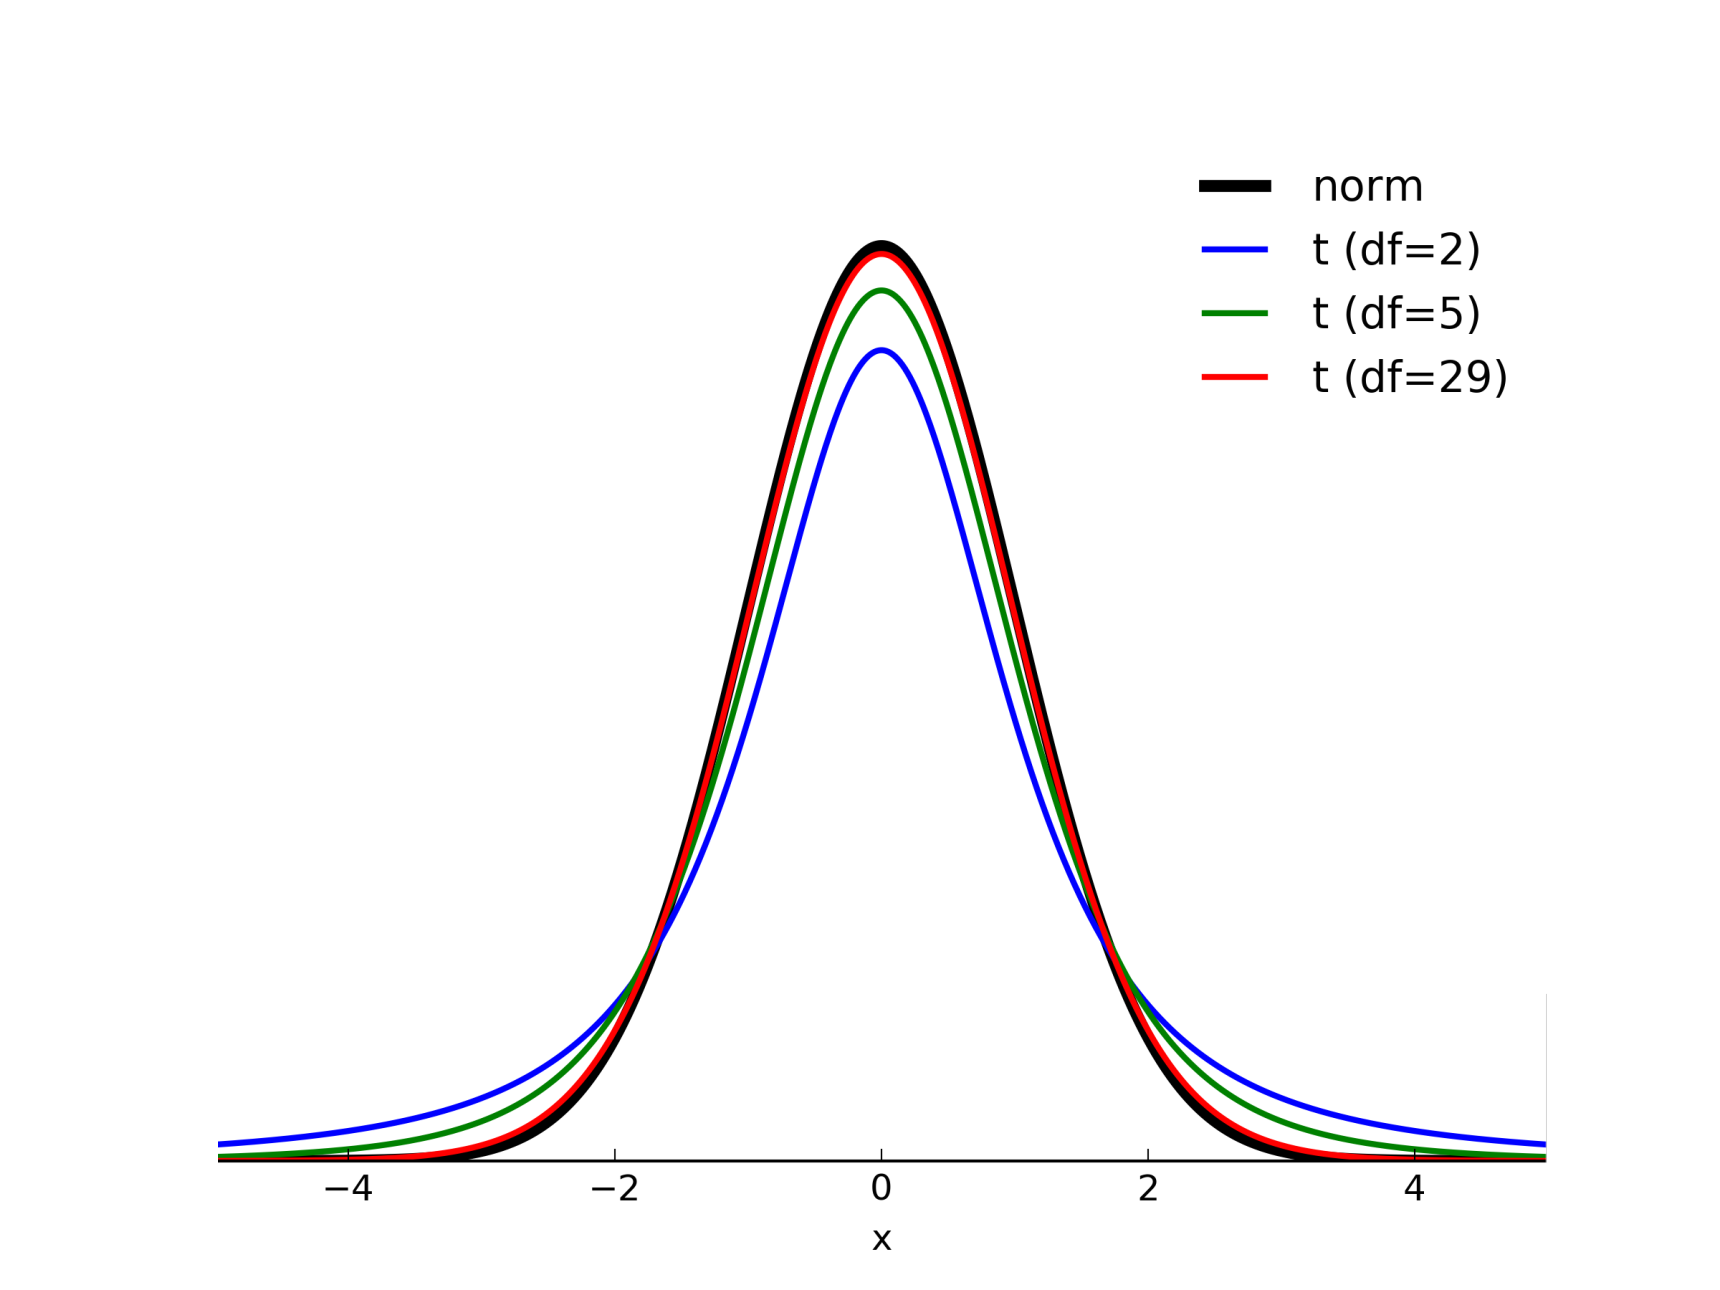
\includegraphics[width=0.75\linewidth]{/Users/craig.starbuck/Library/Mobile Documents/com~apple~CloudDocs/Documents/People Analytics Book/GitHub/peopleanalytics_lifecycle_book/graphics/t_distribution} 

}

\caption{t Distribution Shape by Degrees of Freedom}\label{fig:t-distribution}
\end{figure}

When estimating the CI for smaller samples, we need to leverage the wider, more platykurtic \(t\) distribution to achieve greater accuracy. Therefore, the CI for a two-tailed test in this case is defined by:

\[ CI = \bar{x} \pm t_{\alpha/_2} \frac{\sigma}{\sqrt{n}} \]

Let's compare CIs calculated using a \(t\)-test to those calculated using the Z-Test. While a fixed \(z\) score can be used for each CI level when \(n\) \textgreater{} 30, the \(t\) statistic varies based on both the CI level and \(df\). Though R will determine the correct \(t\) statistic for us, let's reference the table shown in Figure \ref{fig:t-crit} to manually lookup the \(t\) statistic:

\begin{figure}

{\centering 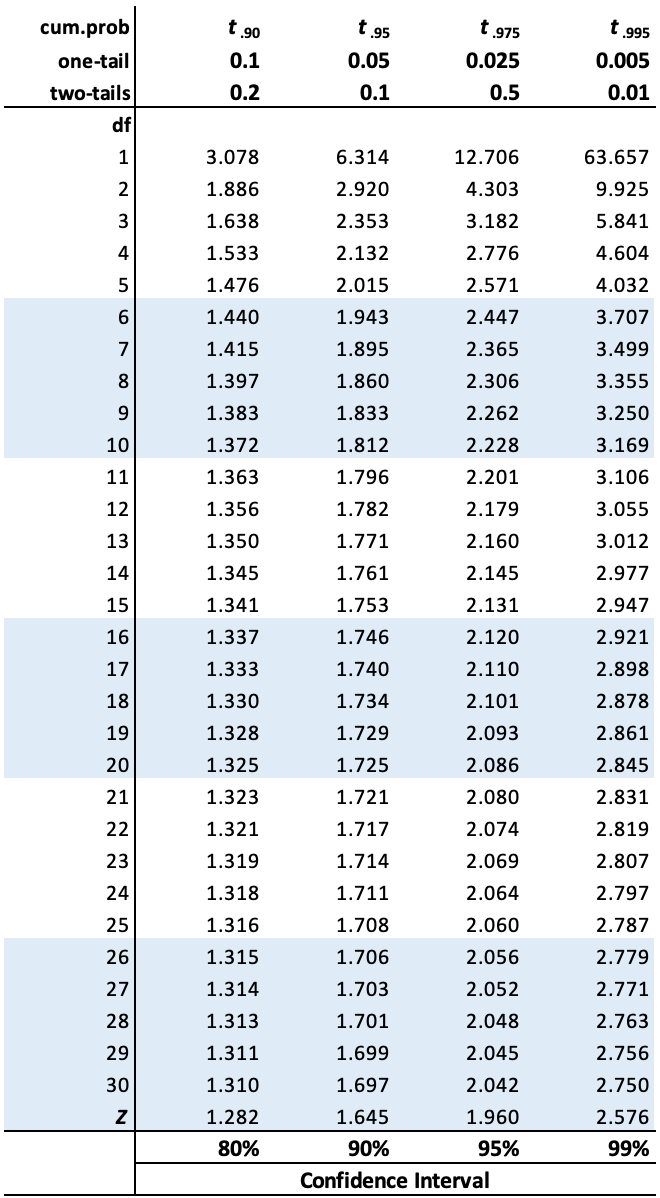
\includegraphics[width=0.5\linewidth]{/Users/craig.starbuck/Library/Mobile Documents/com~apple~CloudDocs/Documents/People Analytics Book/GitHub/peopleanalytics_lifecycle_book/graphics/t-table} 

}

\caption{Critical Values of Student's t Distribution}\label{fig:t-crit}
\end{figure}

For illustrative purposes, let's draw a smaller sample of \(n\) = 25 from our uniform population distribution and calculate the 95\% CI using the \(t\) statistic from the table (\(df\) = 24). The \(t\) statistic for this CI and \(df\) is 2.064:

\begin{Shaded}
\begin{Highlighting}[]
\CommentTok{\# Set seed for reproducible random samples}
\FunctionTok{set.seed}\NormalTok{(}\DecValTok{456}\NormalTok{)}

\CommentTok{\# Sample 25 values from uniform population distribution}
\NormalTok{x }\OtherTok{\textless{}{-}} \FunctionTok{sample}\NormalTok{(rand.unif, }\DecValTok{25}\NormalTok{, }\AttributeTok{replace =} \ConstantTok{TRUE}\NormalTok{, }\AttributeTok{prob =} \ConstantTok{NULL}\NormalTok{)}

\CommentTok{\# Calculate 95\% CI}
\NormalTok{ci95\_lower\_bound }\OtherTok{\textless{}{-}} \FunctionTok{mean}\NormalTok{(x) }\SpecialCharTok{{-}} \FloatTok{2.064} \SpecialCharTok{*}\NormalTok{ (}\FunctionTok{sd}\NormalTok{(x) }\SpecialCharTok{/} \FunctionTok{sqrt}\NormalTok{(}\DecValTok{25}\NormalTok{))}
\NormalTok{ci95\_upper\_bound }\OtherTok{\textless{}{-}} \FunctionTok{mean}\NormalTok{(x) }\SpecialCharTok{+} \FloatTok{2.064} \SpecialCharTok{*}\NormalTok{ (}\FunctionTok{sd}\NormalTok{(x) }\SpecialCharTok{/} \FunctionTok{sqrt}\NormalTok{(}\DecValTok{25}\NormalTok{))}
\end{Highlighting}
\end{Shaded}

\begin{Shaded}
\begin{Highlighting}[]
\CommentTok{\# Print lower bound for 95\% CI}
\NormalTok{ci95\_lower\_bound}
\end{Highlighting}
\end{Shaded}

\begin{verbatim}
## [1] 35.24305
\end{verbatim}

\begin{Shaded}
\begin{Highlighting}[]
\CommentTok{\# Print upper bound for 95\% CI}
\NormalTok{ci95\_upper\_bound}
\end{Highlighting}
\end{Shaded}

\begin{verbatim}
## [1] 59.60959
\end{verbatim}

As expected, the 95\% CI using the \(t\) statistic is much wider (35.2 - 59.6), acknowledging the increased uncertainty in estimating population parameters given the limited information in this smaller sample. To increase our confidence to the 99\% level, the interval widens even further (30.9 - 63.9):

\begin{Shaded}
\begin{Highlighting}[]
\CommentTok{\# Calculate 99\% CI}
\NormalTok{ci99\_lower\_bound }\OtherTok{\textless{}{-}} \FunctionTok{mean}\NormalTok{(x) }\SpecialCharTok{{-}} \FloatTok{2.797} \SpecialCharTok{*}\NormalTok{ (}\FunctionTok{sd}\NormalTok{(x) }\SpecialCharTok{/} \FunctionTok{sqrt}\NormalTok{(}\DecValTok{25}\NormalTok{))}
\NormalTok{ci99\_upper\_bound }\OtherTok{\textless{}{-}} \FunctionTok{mean}\NormalTok{(x) }\SpecialCharTok{+} \FloatTok{2.797} \SpecialCharTok{*}\NormalTok{ (}\FunctionTok{sd}\NormalTok{(x) }\SpecialCharTok{/} \FunctionTok{sqrt}\NormalTok{(}\DecValTok{25}\NormalTok{))}
\end{Highlighting}
\end{Shaded}

\begin{Shaded}
\begin{Highlighting}[]
\CommentTok{\# Print lower bound for 99\% CI}
\NormalTok{ci99\_lower\_bound}
\end{Highlighting}
\end{Shaded}

\begin{verbatim}
## [1] 30.91633
\end{verbatim}

\begin{Shaded}
\begin{Highlighting}[]
\CommentTok{\# Print upper bound for 99\% CI}
\NormalTok{ci99\_upper\_bound}
\end{Highlighting}
\end{Shaded}

\begin{verbatim}
## [1] 63.93631
\end{verbatim}

\hypertarget{hypothesis-testing}{%
\subsection{Hypothesis Testing}\label{hypothesis-testing}}

\textbf{Hypothesis testing} is how we leverage CIs to test whether a significant difference or relationship exists in the data. Sir Ronald Fisher invented what is known as the null hypothesis, which states that there is no relationship/difference; disprove me if you can! The null hypothesis is defined by:

\[ H_0: \mu_A = \mu_B \]

The objective of hypothesis testing is to determine if there is sufficient evidence to reject the null hypothesis in favor of an alternative hypothesis. The null hypothesis always states that there is `nothing' of significance. For example, if we want to test whether an intervention has an effect on an outcome in a population, the null hypothesis states that there is no effect. If we want to test whether there is a difference in average scores between two groups in a population, the null hypothesis states that there is no difference.

An alternative hypothesis may simply state that there is a difference or relationship in the population, or it may specify the expected direction (e.g., Population A has a significantly `larger' or `smaller' average value than Population B; Variable A is `positively' or `negatively' related to Variable B). Therefore, alternative hypotheses are defined by:

\[ H_A: \mu_A \neq \mu_B \]

\[ H_A: \mu_A < \mu_B \]

\[ H_A: \mu_A > \mu_B \]

\hypertarget{alpha}{%
\subsection{Alpha}\label{alpha}}

The \textbf{alpha} level of a hypothesis test, denoted by \(\alpha\), represents the probability of obtaining observed results due to chance if the null hypothesis is true. In other words, \(\alpha\) is the probability of rejecting the null hypothesis (and therefore claiming that there is a significant difference or relationship) when in fact we should have failed to reject it because there is insufficient evidence to support the alternative hypothesis.

\(\alpha\) is often set at .05 but is sometimes set at a more rigorous .01, depending upon the context and tolerance for error. An \(\alpha\) of .05 corresponds to a 95\% CI (1 - .05), and .01 to a 99\% CI (1 - .01). With non-directional alternative hypotheses, we must divide \(\alpha\) by 2 (i.e., we could observe a significant result in either tail of the distribution), while one-tailed tests position the rejection region entirely within one tail based on what is being hypothesized.

At the .05 level, we would conclude that a finding is statistically significant if the chance of observing a value at least as extreme as the one observed is less than 1 in 20 if the null hypothesis is true. Note that we observed this behavior with our simulated distribution of sample means. While we could observe more extreme values by chance with repeated attempts, in less than 1 in every 20 times would we expect a 95\% CI that does not capture \(\mu\). Moreover, in less than 1 in every 100 times should we expect a sample with a 99\% CI that does not capture \(\mu\).

\hypertarget{type-i-ii-errors}{%
\subsection{Type I \& II Errors}\label{type-i-ii-errors}}

A \textbf{Type I Error} is a false positive, wherein we conclude that there is a significant difference or relationship when there is not. A \textbf{Type II Error} is a false negative, wherein we fail to capture a significant finding. \(\alpha\) represents our chance of making a Type I Error, while \(\beta\) represents our chance of making a Type II Error. I once had a professor explain that committing a Type I error is a shame, while committing a Type II error is a pity, and I've found this to be a helpful way to remember what each type of error represents.

\begin{figure}

{\centering 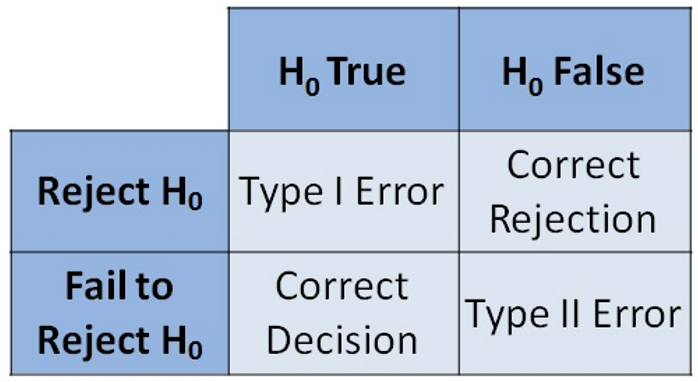
\includegraphics[width=0.5\linewidth]{/Users/craig.starbuck/Library/Mobile Documents/com~apple~CloudDocs/Documents/People Analytics Book/GitHub/peopleanalytics_lifecycle_book/graphics/hypothesis_testing_errors} 

}

\caption{Type I and II Errors}\label{fig:hyp-errs}
\end{figure}

\hypertarget{p-values}{%
\subsection{\texorpdfstring{\(p\)-Values}{p-Values}}\label{p-values}}

In statistical tests, the \textbf{p-value} is referenced to determine whether the null hypothesis can be rejected. The p-value represents the probability of obtaining a result at least as extreme as the one observed if the null hypothesis is true. As a general rule, if \(p\) \textless{} .05, we can confidently reject the null hypothesis and conclude that the observed difference or relationship was unlikely a chance observation.

While statistical significance helps us understand the probability of observing results by chance when there is no difference or effect in the population, it does not tell us anything about the size of the difference or effect. Analysis should never be reduced to inspecting p-values; in fact, p-values have been the subject of much controversy among researchers and practitioners in recent years. Later chapters will cover how to interpret results of statistical tests to surface the story and determine if there is anything `practically' significant among statistically significant findings.

\hypertarget{bonferroni-correction}{%
\subsection{Bonferroni Correction}\label{bonferroni-correction}}

One caveat when leveraging a p-value to determine statistical significance is that when multiple testing is performed -- that is, multiple tests using the same sample data -- the probability of a Type I error increases by a factor equivalent to the number of tests performed. It's important to note that there is not agreement among statisticians about how (or even whether) the p-value threshold for statistical significance needs to be adjusted to account for this increased risk. Nevertheless, we will cover this conservative approach for mitigating this risk.

Thus far, we have only discussed statistical significance in the context of a \textbf{per analysis error rate} -- that is, the probability of committing a Type I error for a single statistical test. However, when two or more tests are being conducted on the same sample, the \textbf{familywise error rate} is an important factor in determining statistical significance. The familywise error rate reflects the fact that as we conduct more and more analyses on the same sample, the probability of a Type I error across the set (or family) of analyses increases. The familywise error rate can be calculated by:

\[ \alpha_{FW} = 1 - (1 - \alpha_{PC})^C,  \]

where \(c\) is equal to the number of comparisons (or statistical tests) performed, and \(\alpha_{PC}\) is equal to the specified per analysis error rate (usually .05). For example, if \(\alpha\) = .05 per analysis, the probability of a Type I error with three tests on the same data increases from 5\% to 14.3\%: \(1 - (1 - .05)^3 = .143\).

The most common method of adjusting the familywise error rate down to the specified per analysis error rate is the \textbf{Bonferroni Correction}. To implement this correction, we can simply divide \(\alpha\) by the number of analyses performed on the dataset -- such as \(\alpha / 3 = .017\) in the case of three analyses with \(\alpha = .05\). This means that for each statistical test, we must achieve \(p < .017\) to report a statistically significant result. An alternative which allows us to achieve the same number of statistically significant results is to multiply the unadjusted per analysis p-values for each statistical test by the number of tests. For example, if we run three statistical tests and receive \(p = .014\), \(p = .047\), and \(p = .125\), we would achieve one significant result with the first method (\(p < .017\)) as well as with the alternative since the first statistical test satisfies the per analysis error rate (\(p < .05\)): \(p = .014 * 3 = .042\).

Perneger (1998) is one of many who oppose the use of the Bonferroni Correction, suggesting that these ``adjustments are, at best, unnecessary and, at worst, deleterious to sound statistical inference.'' The Bonferroni Correction is controversial among researchers because while applying the correction reduces the chance of a Type I error, it also increases the chance of a Type II error. Because this correction makes it more difficult to detect significant results, it is rare to find such a correction reported in published research, though research often involves multiple testing on the same sample. Perneger suggests that simply describing the statistical tests that were performed, and why, is sufficient for dealing with potential problems introduced by multiple testing.

\hypertarget{statistical-power}{%
\subsection{Statistical Power}\label{statistical-power}}

Whereas \(\alpha\) is the probability of a Type I error, \textbf{Beta} \(\beta\) is the opposite: the probability of accepting \(H_0\) when it is false (Type II error).

\(\beta\) is related to the \emph{power} of the analysis, which is calculated by 1 - \(\beta\) and reflects our ability to detect a difference or relationship if one exists. For example, if a study has 80\% power, it has an 80\% chance of detecting an effect if one actually exists in the population. \textbf{Power analysis} helps with defining the optimal \(n\)-count for detecting a population effect in sample data (i.e., correctly rejecting a false \(H_0\)). Increasing the power of a statistical test decreases the probability that we will fail to detect a significant effect present in the population.

At this point, it should be intuitive that larger samples increase our chances of observing significant results. As we observed in the \(t\)-test example, CIs for small samples (\(n\) \textless{} 30) are quite wide relative to those for large samples; therefore, the power of the analysis to detect significance is limited given how different the values of \(x\) must be to observe non-overlapping CIs.

Before diving into the mechanics of power analysis, it is important to understand the three important -- and interrelated -- considerations in hypothesis tests that influence whether effects are real or a product of random sampling error:

\begin{itemize}
\tightlist
\item
  \textbf{Effect size}: Larger differences and stronger relationships are less likely random sampling error
\item
  \textbf{Sample size}: Larger samples can detect smaller differences and weaker relationships (though they may be too small or weak to be meaningful)
\item
  \textbf{Variability}: Greater variability in the data is likely to result in differences that are attributable to random sampling error
\end{itemize}

It may be helpful to think of power analysis as an optimization problem. The goal is to achieve a large enough sample size to detect meaningful effects -- but not wastefully large as data collection can be expensive -- whilst protecting against an underpowered analysis with a low probability of detecting an important effect.

To estimate the sample size needed to achieve a given power level, one must use domain expertise to specify parameters. The effect size parameter varies based on the statistical test but when in doubt, we can use Cohen's (1988) conventional effect sizes which are defined in Figure \ref{fig:conv-eff-size-tbl}. The effect size for a particular test can also be retrieved using the \texttt{cohen.ES()} function. For example, the following command returns 0.25 as the medium effect size threshold for ANOVA: \texttt{cohen.ES(test\ =\ "anov",\ size\ =\ "medium")}.

\begin{figure}

{\centering 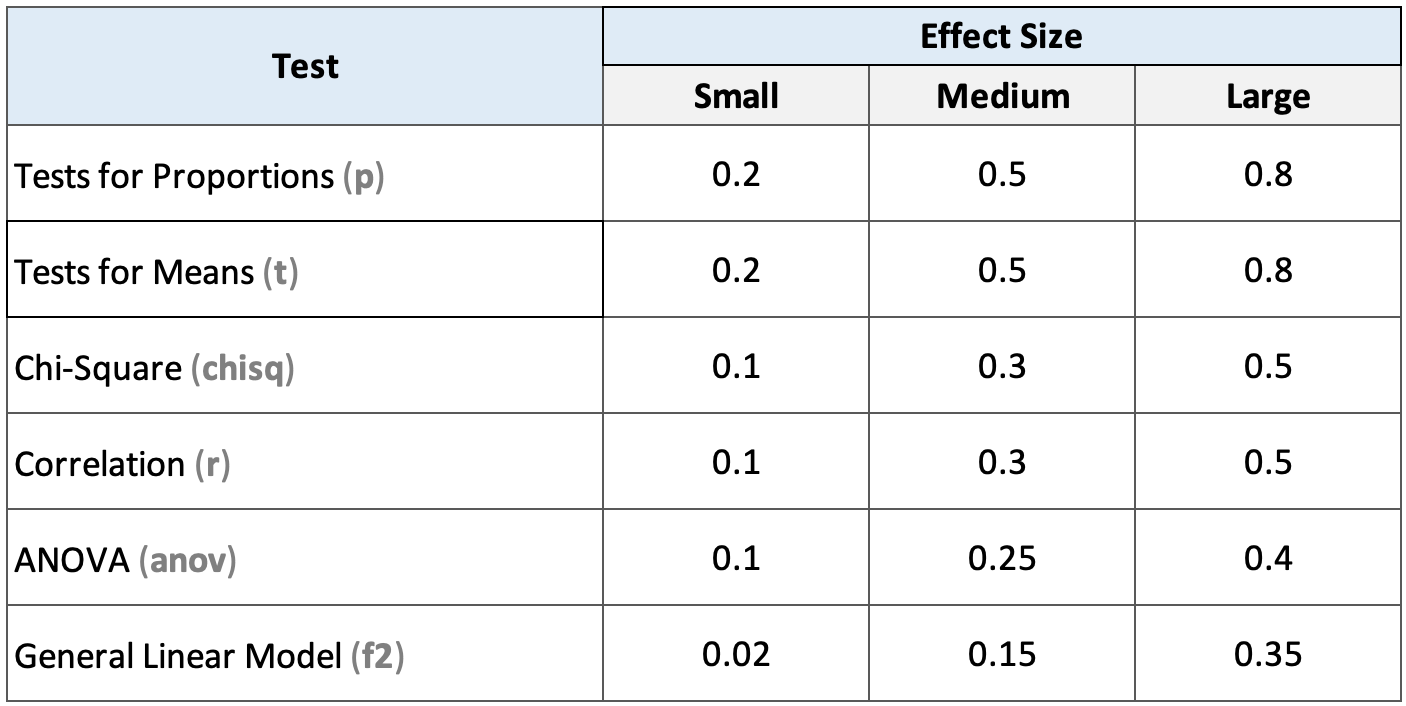
\includegraphics[width=1\linewidth]{/Users/craig.starbuck/Library/Mobile Documents/com~apple~CloudDocs/Documents/People Analytics Book/GitHub/peopleanalytics_lifecycle_book/graphics/conventional_effect_size_table} 

}

\caption{Cohen's conventional effect sizes by statistical test.}\label{fig:conv-eff-size-tbl}
\end{figure}

Let's illustrate by calculating the sample size required for a one-way ANOVA that involves four groups. We will set \(\alpha = .05\) and specify an 80\% chance (power = .8) of detecting a moderate population effect. We can leverage the \texttt{pwr} library in R to perform power analysis. Executing \texttt{?pwr} will provide package documentation that clarifies what function to execute to calculate the sample size requirement for various statistical tests.

\begin{Shaded}
\begin{Highlighting}[]
\CommentTok{\# Load library}
\FunctionTok{library}\NormalTok{(pwr)}

\CommentTok{\# Calculate sample size for one{-}way ANOVA}
\CommentTok{\# k = 4 indicates we plan to compare 4 groups}
\CommentTok{\# f = .25 indicates we wish to detect a medium effect}
\FunctionTok{pwr.anova.test}\NormalTok{(}\AttributeTok{k =} \DecValTok{4}\NormalTok{, }\AttributeTok{f =}\NormalTok{ .}\DecValTok{25}\NormalTok{, }\AttributeTok{sig.level =}\NormalTok{ .}\DecValTok{05}\NormalTok{, }\AttributeTok{power =}\NormalTok{ .}\DecValTok{8}\NormalTok{)}
\end{Highlighting}
\end{Shaded}

\begin{verbatim}
## 
##      Balanced one-way analysis of variance power calculation 
## 
##               k = 4
##               n = 44.59927
##               f = 0.25
##       sig.level = 0.05
##           power = 0.8
## 
## NOTE: n is number in each group
\end{verbatim}

The power analysis for this one-way ANOVA shows that we need a minimum of \(n = 45\) \emph{within each} of the four groups to achieve an 80\% chance of detecting a medium population effect across the four groups when setting \(\alpha = .05\).

\hypertarget{review-questions-5}{%
\section{Review Questions}\label{review-questions-5}}

\begin{enumerate}
\def\labelenumi{\arabic{enumi}.}
\item
  What are some examples of a null hypothesis?
\item
  What is the difference between Type I and Type II errors?
\item
  What is the primary purpose of inferential statistics, and how does it differ from descriptive statistics?
\item
  What is the Central Limit Theorem (CLT), and why is it important?
\item
  Is randomness a requirement for probabilistic methods? Why or why not?
\item
  What does the Bonferroni Correction seek to achieve?
\item
  What is a confidence interval (CI)?
\item
  What are some examples of how the context influences what level of confidence is appropriate for statistical significance testing? Should we always use a 95 CI?
\item
  When population parameters are unknown, which test would be appropriate for testing the following null hypothesis: \(\mu_A = \mu_B\)?
\item
  According to the Empirical Rule, 95\% of normally distributed data lie within how many standard deviations of the mean?
\end{enumerate}

\hypertarget{data-mgmt-prep}{%
\chapter{Data Management \& Preparation}\label{data-mgmt-prep}}

To begin a data analysis, we must first access and organize the relevant data. These tasks -- together with data preparation steps outlined in this chapter -- account for a large part of the work analytics professionals do.

\begin{figure}

{\centering 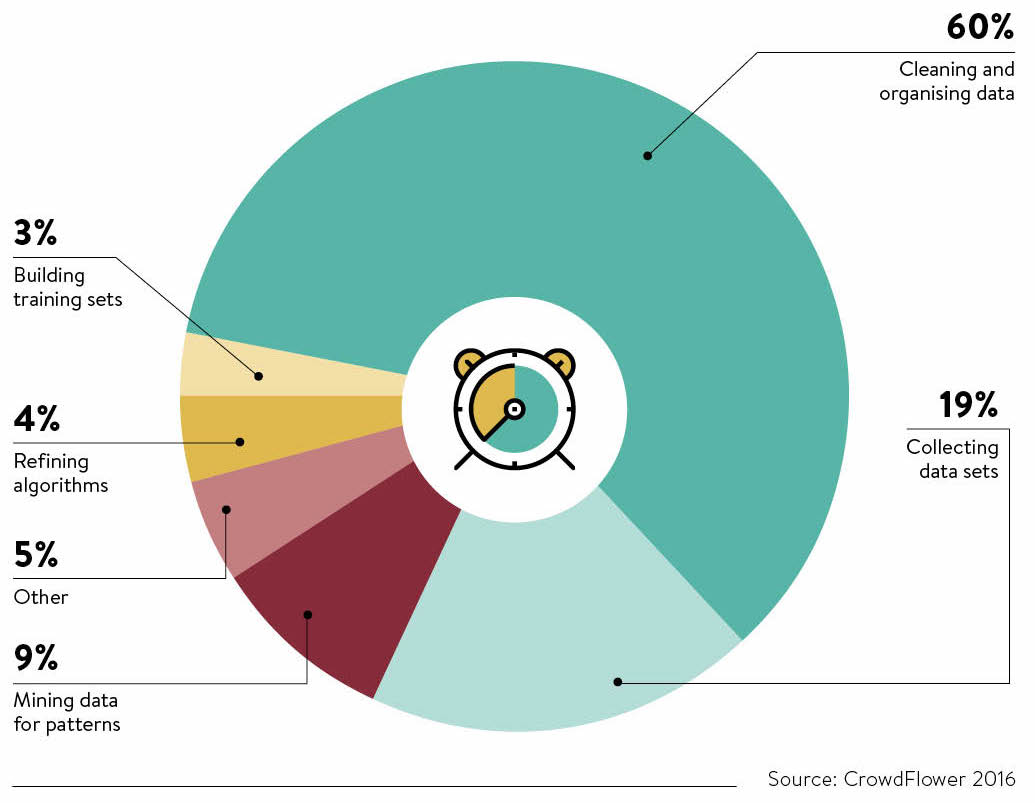
\includegraphics[width=0.75\linewidth]{/Users/craig.starbuck/Library/Mobile Documents/com~apple~CloudDocs/Documents/People Analytics Book/GitHub/peopleanalytics_lifecycle_book/graphics/data_scientist_tasks} 

}

\caption{What Data Scientists Really Do}\label{fig:ds-tasks}
\end{figure}

\hypertarget{data-management}{%
\section{Data Management}\label{data-management}}

Data are generally extracted directly from the source systems in which they are generated or from downstream repositories such as a \emph{data lake}, \emph{data warehouse}, or \emph{data mart}. To properly and efficiently extract data -- often through the use of SQL as covered in Chapter \ref{sql-intro} -- it is important to first understand some of the most common ways in which data are stored and structured.

A \textbf{data lake} stores myriad types of data -- both structured and unstructured -- in its native format until needed. \textbf{Structured data} refers to data that fits a predefined data model, such as hire dates formatted as \texttt{MM/DD/YYYY} or zip codes stored as a five-digit string. \textbf{Unstructured data} has no predefined data model, such as audio and video files, free-form performance review comments, emails, or digital exhaust from messaging tools; it is difficult to structure this type of data within a set of related tables.

The main difference between a data lake and data warehouse is the type of data they are designed to store. A \textbf{data warehouse (DW)} is designed to support analytics across large collections of data, such as transactional data (e.g., point-of-sale systems), point-in-time snapshots (e.g., month-end close reports), survey responses, spreadsheets, and more. As shown in Figure \ref{fig:dw-schema}, data in a DW are structured and organized into schemas of related tables to enhance the performance of queries spanning sets of large and diverse data.

Figure \ref{fig:dw-schema} illustrates how worker, position, and recruiting schemas may be related. For example, a candidate submits a job application to a posted requisition, which is connected to an open position Finance approved as part of the company's workforce plan; when the selected candidate is hired, they become a worker with one or many events (hire, promotion, transfer, termination) and activities (learning, performance appraisals, surveys) during their tenure with the company.

\begin{figure}

{\centering 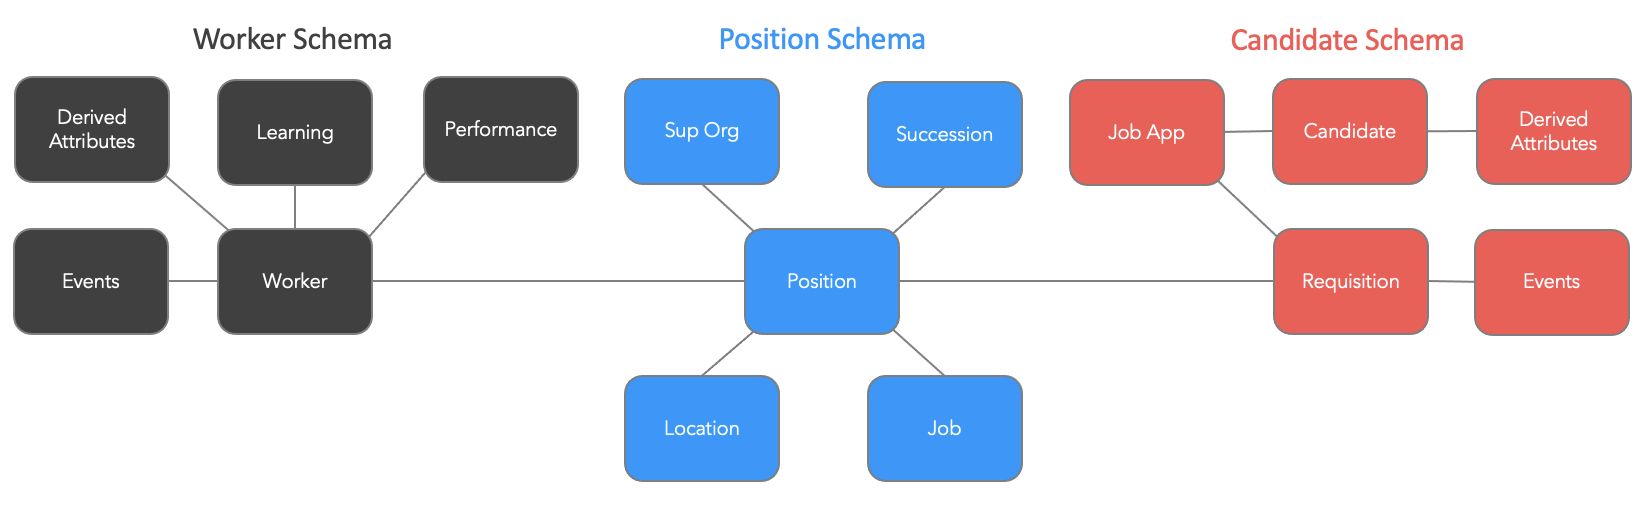
\includegraphics[width=1\linewidth]{/Users/craig.starbuck/Library/Mobile Documents/com~apple~CloudDocs/Documents/People Analytics Book/GitHub/peopleanalytics_lifecycle_book/graphics/dw_schema} 

}

\caption{Related Tables Organized within Schemas}\label{fig:dw-schema}
\end{figure}

Tables in a DW are related using a set of keys. Each table needs a \textbf{Primary Key (PK)}, which is a unique identifier for each row in the table. A PK may be a single column or multiple columns; a multi-column PK is often referred to as a \emph{composite key}. It is generally best to leverage non-recyclable system-generated ids for PKs, as descriptors like names tend to be unreliable. A \textbf{Foreign Key (FK)} is a column whose values correspond to the values of a PK in another table. \textbf{Referential integrity} is the logical dependency of a FK on a PK, and these constraints protect against orphaned FK values in child tables by deleting PK values from an associated parent table.

Figure \ref{fig:dw-erd} shows an \textbf{Entity Relationship Diagram (ERD)} that depicts PK/FK relationships among the Position, Worker, and Requisition tables. Notice that the PK of each related table shown in Figure \ref{fig:dw-schema} is listed as a FK.

\begin{figure}

{\centering 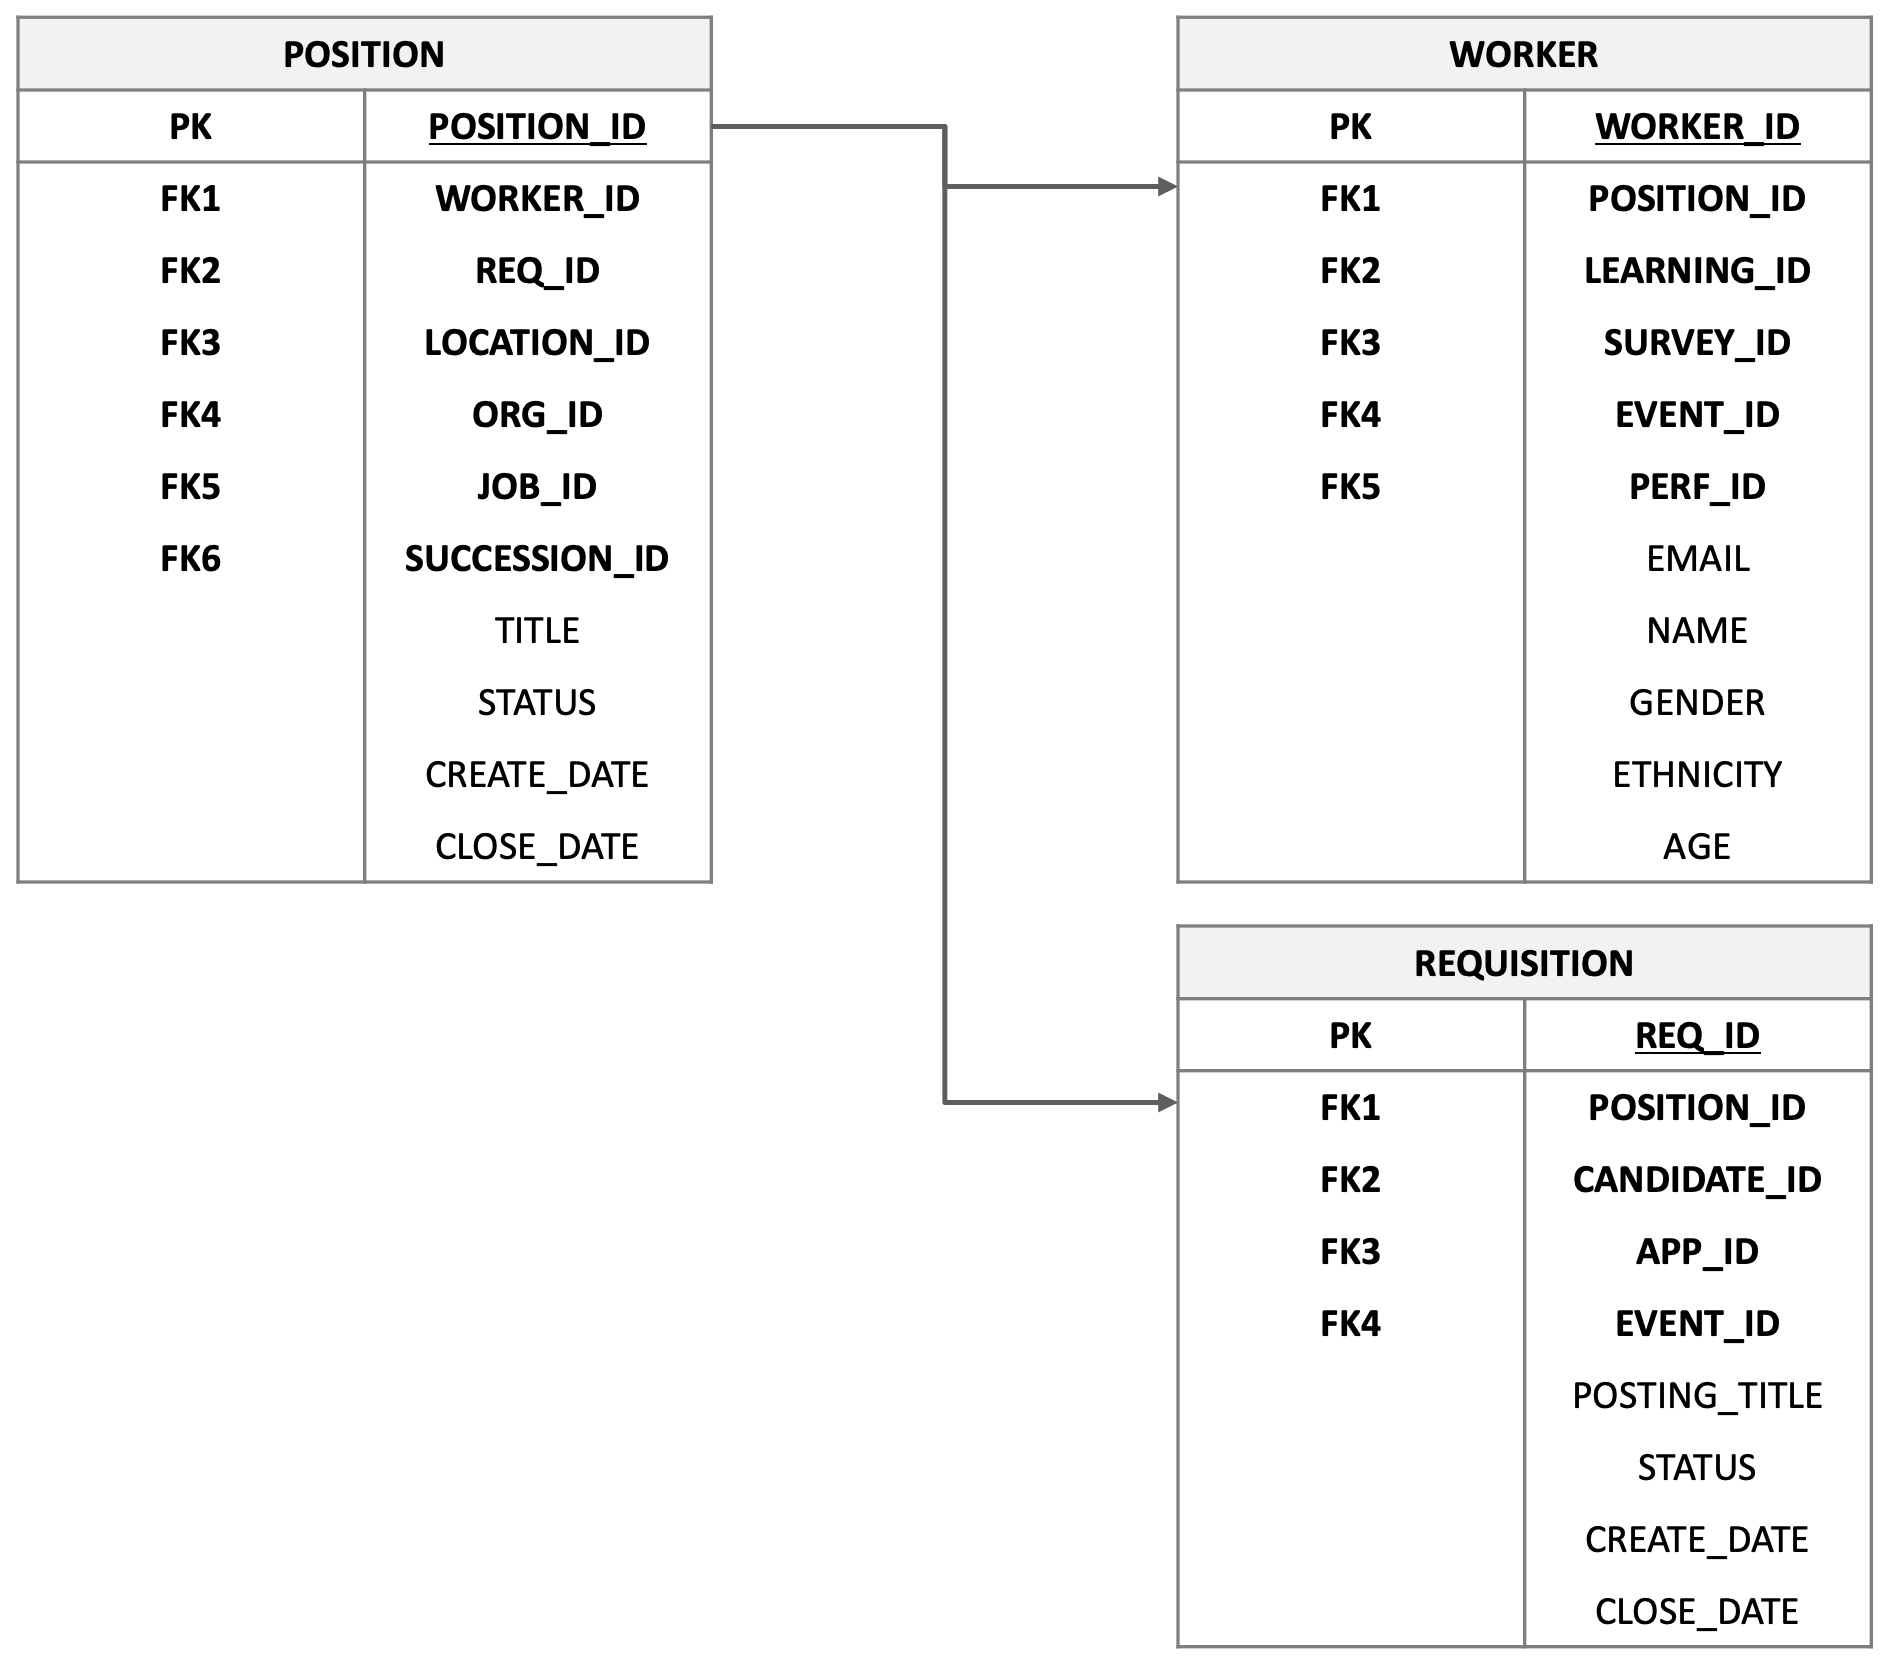
\includegraphics[width=0.75\linewidth]{/Users/craig.starbuck/Library/Mobile Documents/com~apple~CloudDocs/Documents/People Analytics Book/GitHub/peopleanalytics_lifecycle_book/graphics/dw_erd} 

}

\caption{Entity Relationship Diagram (ERD)}\label{fig:dw-erd}
\end{figure}

A DW may contain many different types of tables, but this chapter will focus on the two most common which are known as \emph{Type 1} and \emph{Type 2} tables. These tables are sometimes referred to as \textbf{slowly changing dimensions (SCD)}. A \textbf{Type 1 table} is overwritten on a regular cadence (usually daily) and contains no history -- only current values. For example, a Type 1 table may contain the latest known attributes for each active and terminated worker such as job, location, and manager. A Type 1 table is convenient when only current information needs to be queried. A \textbf{Type 2 table} is a table in which a new record is inserted when a change occurs for one or more specified dimensions. Jobs, managers, and locations are examples of slowly changing dimensions but unlike the Type 1 table which contains only the latest information, the Type 2 table houses a \emph{start date} and \emph{end date} for each worker and dimension to facilitate reporting and analysis on changes to attribute values over time.

Figure \ref{fig:type-2-tbl} illustrates the design of a Type 2 SCD for an active worker's job, manager, and location changes. As the data show, worker 123 was promoted from Data Analyst to Sr.~Data Analyst 1.5 years after joining, began reporting to their original manager (456) after a short stint reporting to someone else (789), and has worked remotely throughout their tenure with the company.

Note that the combination of \texttt{end\_date\ =\ \textquotesingle{}12/31/9999\textquotesingle{}} and \texttt{current\_record\ =\ \textquotesingle{}Y\textquotesingle{}} indicate \emph{current attributes} for active workers. For inactive workers, \texttt{end\_date} is set to the worker's termination date for rows that represent the \emph{last known attributes} along with \texttt{current\_record\ =\ \textquotesingle{}Y\textquotesingle{}}:

\begin{figure}

{\centering 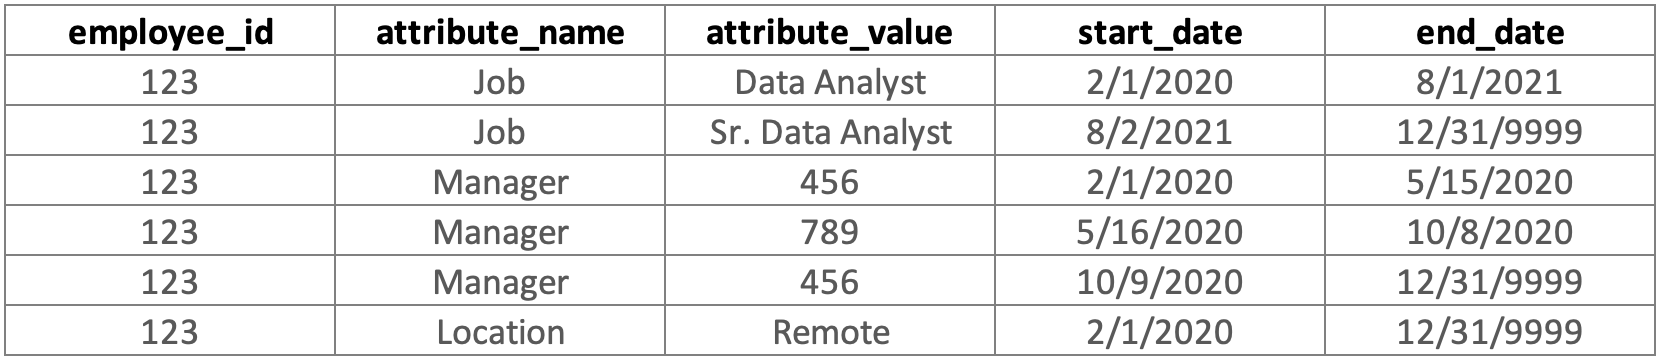
\includegraphics[width=1\linewidth]{/Users/craig.starbuck/Library/Mobile Documents/com~apple~CloudDocs/Documents/People Analytics Book/GitHub/peopleanalytics_lifecycle_book/graphics/type_2_table} 

}

\caption{Type 2 SCD}\label{fig:type-2-tbl}
\end{figure}

While we could select rows where \texttt{current\_record\ =\ \textquotesingle{}Y\textquotesingle{}} to construct a view of the last known attributes for each worker in this table, the task would be unnecessarily complex. Using a Type 1 table simplifies the task and output since each dimension value is stored in a separate column and there is only one row per employee. Figure \ref{fig:type-1-tbl} shows how the current record for worker 123 would look in a Type 1 SCD:

\begin{figure}

{\centering 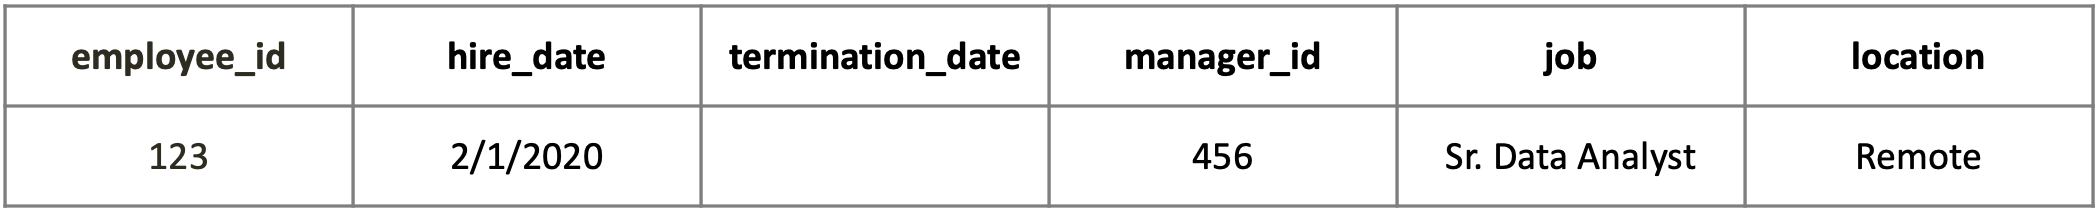
\includegraphics[width=1\linewidth]{/Users/craig.starbuck/Library/Mobile Documents/com~apple~CloudDocs/Documents/People Analytics Book/GitHub/peopleanalytics_lifecycle_book/graphics/type_1_table} 

}

\caption{Type 1 SCD}\label{fig:type-1-tbl}
\end{figure}

A \textbf{data mart} is a subset of a DW designed to easily deliver specific information to a certain set of users on a particular subject or for a well-defined use case. For example, in a people analytics context a diversity data mart could be developed to better isolate and secure restricted data such as gender and ethnicity. This data may be used to support diversity descriptives and trends for a limited audience approved by Data Privacy and Employment Law counsel based on justified business needs.

\textbf{Modern Data Architecture}

Though a deep treatment of data architecture is beyond the scope of this book, it is important to acknowledge the significant advancements in infrastructure and computation since these complex SCD architectures were introduced by Kimball (1996). These developments have greatly improved the efficiency with which analysts can translate data into information and insight. The primitive systems in place decades ago required expensive \textbf{ETL} jobs to \textbf{extract (E)} data from source systems, \textbf{transform (T)} data using complex transformation rules, and \textbf{load (L)} the transformed data to relational tables -- which then required complex queries to wrangle and analyze the data.

With modern cloud environments, the significant investment associated with humans designing, developing, and maintaining these complex architectures is often difficult to justify given how inexpensive storage and compute have become. Increasingly, the heavy computational tasks have migrated out of data pipelines and into the analytics layer wherein analytics teams have more flexibility and control. Today, daily snapshots containing \emph{all} current and historical records can be copied and stored within partitioned DW tables for a negligible increase in storage costs, and this greatly simplifies data pipeline complexity and engineering support requirements. This changing dynamic has given rise to a new breed of data engineers focused on optimizing the heavy computation requirements of analytics teams.

\hypertarget{data-screening-cleaning}{%
\section{Data Screening \& Cleaning}\label{data-screening-cleaning}}

The initial data review process is sometimes referred to as \textbf{exploratory data analysis (EDA)}. EDA involves investigating patterns, completeness, anomalies, and assumptions using summary statistics and graphical representations. An analytics ideal is \emph{unimpeachable data quality}, which is to say that the rigor of upstream processes and downstream data screening is such that stakeholders become confident enough to channel more energy towards actioning on results than questioning the quality. Suspect data quality is often surfaced during the initial EDA step and affords the opportunity to address and avoid stakeholders discounting results during later phases of the project.

A handy function in base R for initial data screening is \texttt{summary()}:

\begin{Shaded}
\begin{Highlighting}[]
\CommentTok{\# Load employee data}
\NormalTok{employees }\OtherTok{\textless{}{-}} \FunctionTok{read.csv}\NormalTok{(}\StringTok{"/Users/craig.starbuck/Library/Mobile Documents/com\textasciitilde{}apple\textasciitilde{}CloudDocs/Documents/People Analytics Book/GitHub/peopleanalytics\_lifecycle\_book/data/employees.csv"}\NormalTok{)}

\CommentTok{\# Summarize df}
\FunctionTok{summary}\NormalTok{(employees)}
\end{Highlighting}
\end{Shaded}

\begin{verbatim}
##   employee_id      active          stock_opt_lvl      trainings    
##  Min.   :1001   Length:1470        Min.   :0.0000   Min.   :0.000  
##  1st Qu.:1368   Class :character   1st Qu.:0.0000   1st Qu.:2.000  
##  Median :1736   Mode  :character   Median :1.0000   Median :3.000  
##  Mean   :1736                      Mean   :0.7939   Mean   :2.799  
##  3rd Qu.:2103                      3rd Qu.:1.0000   3rd Qu.:3.000  
##  Max.   :2470                      Max.   :3.0000   Max.   :6.000  
##                                                                    
##       age         commute_dist        ed_lvl        ed_field        
##  Min.   :18.00   Min.   : 1.000   Min.   :1.000   Length:1470       
##  1st Qu.:30.00   1st Qu.: 2.000   1st Qu.:2.000   Class :character  
##  Median :36.00   Median : 7.000   Median :3.000   Mode  :character  
##  Mean   :36.92   Mean   : 9.193   Mean   :2.913                     
##  3rd Qu.:43.00   3rd Qu.:14.000   3rd Qu.:4.000                     
##  Max.   :60.00   Max.   :29.000   Max.   :5.000                     
##                                                                     
##     gender          marital_sts            dept             engagement  
##  Length:1470        Length:1470        Length:1470        Min.   :1.00  
##  Class :character   Class :character   Class :character   1st Qu.:2.00  
##  Mode  :character   Mode  :character   Mode  :character   Median :3.00  
##                                                           Mean   :2.73  
##                                                           3rd Qu.:3.00  
##                                                           Max.   :4.00  
##                                                                         
##     job_lvl       job_title           overtime         business_travel   
##  Min.   :1.000   Length:1470        Length:1470        Length:1470       
##  1st Qu.:1.000   Class :character   Class :character   Class :character  
##  Median :2.000   Mode  :character   Mode  :character   Mode  :character  
##  Mean   :2.064                                                           
##  3rd Qu.:3.000                                                           
##  Max.   :5.000                                                           
##                                                                          
##   hourly_rate       daily_comp     monthly_comp    annual_comp    
##  Min.   : 30.00   Min.   :240.0   Min.   : 5200   Min.   : 62400  
##  1st Qu.: 48.00   1st Qu.:384.0   1st Qu.: 8320   1st Qu.: 99840  
##  Median : 66.00   Median :528.0   Median :11440   Median :137280  
##  Mean   : 65.89   Mean   :527.1   Mean   :11421   Mean   :137054  
##  3rd Qu.: 83.75   3rd Qu.:670.0   3rd Qu.:14517   3rd Qu.:174200  
##  Max.   :100.00   Max.   :800.0   Max.   :17333   Max.   :208000  
##                                                                   
##    ytd_leads       ytd_sales       standard_hrs salary_hike_pct  perf_rating   
##  Min.   :11.00   Min.   : 15496   Min.   :80    Min.   :11.00   Min.   :3.000  
##  1st Qu.:45.00   1st Qu.: 56997   1st Qu.:80    1st Qu.:12.00   1st Qu.:3.000  
##  Median :59.00   Median : 73505   Median :80    Median :14.00   Median :3.000  
##  Mean   :55.84   Mean   : 77124   Mean   :80    Mean   :15.21   Mean   :3.154  
##  3rd Qu.:65.00   3rd Qu.: 96002   3rd Qu.:80    3rd Qu.:18.00   3rd Qu.:3.000  
##  Max.   :95.00   Max.   :281499   Max.   :80    Max.   :25.00   Max.   :4.000  
##  NA's   :1061    NA's   :1061                                                  
##  prior_emplr_cnt    env_sat         job_sat         rel_sat     
##  Min.   :0.000   Min.   :1.000   Min.   :1.000   Min.   :1.000  
##  1st Qu.:1.000   1st Qu.:2.000   1st Qu.:2.000   1st Qu.:2.000  
##  Median :2.000   Median :3.000   Median :3.000   Median :3.000  
##  Mean   :2.693   Mean   :2.722   Mean   :2.729   Mean   :2.712  
##  3rd Qu.:4.000   3rd Qu.:4.000   3rd Qu.:4.000   3rd Qu.:4.000  
##  Max.   :9.000   Max.   :4.000   Max.   :4.000   Max.   :4.000  
##                                                                 
##    wl_balance       work_exp       org_tenure       job_tenure    
##  Min.   :1.000   Min.   : 0.00   Min.   : 0.000   Min.   : 0.000  
##  1st Qu.:2.000   1st Qu.: 6.00   1st Qu.: 3.000   1st Qu.: 2.000  
##  Median :2.000   Median :10.00   Median : 5.000   Median : 3.000  
##  Mean   :1.841   Mean   :11.28   Mean   : 7.032   Mean   : 4.229  
##  3rd Qu.:2.000   3rd Qu.:15.00   3rd Qu.: 9.000   3rd Qu.: 7.000  
##  Max.   :2.000   Max.   :40.00   Max.   :72.000   Max.   :18.000  
##                                                                   
##    last_promo       mgr_tenure     interview_rating
##  Min.   : 0.000   Min.   : 0.000   Min.   :2.000   
##  1st Qu.: 0.000   1st Qu.: 2.000   1st Qu.:3.600   
##  Median : 1.000   Median : 3.000   Median :4.100   
##  Mean   : 2.188   Mean   : 4.123   Mean   :3.989   
##  3rd Qu.: 3.000   3rd Qu.: 7.000   3rd Qu.:4.500   
##  Max.   :15.000   Max.   :17.000   Max.   :5.000   
## 
\end{verbatim}

Note that fields with \texttt{NA\textquotesingle{}s} contain missing values. Also, by default \texttt{employee\_id} is treated as an integer in R, which is why descriptive statistics appropriate for numeric data are provided. \texttt{employee\_id} should actually be treated as a character string since we will not perform any arithmetic operations using these ids.

\textbf{Missingness}

Before considering whether and how to handle missing data, it is important to distinguish between \emph{structural missingness} and \emph{informative missingness} (Kuhn \& Johnson, 2013).

\textbf{Structural missingness} relates to data that are missing for a logical reason. For example, we would not expect a new joiner with a few days of tenure to have a performance score. Likewise, we would not expect an active employee who is not a rehire to have a termination date. Therefore, it would not make sense to define a value to address missing data in these cases.

\textbf{Informative missingness} relates to missing data that is informative regarding an outcome of interest. For example, in a survey context we may find a relationship between missing values on manager effectiveness questions and unfavorability on a psychological safety scale. This may indicate that employees who are fearful of retaliation are uncomfortable providing honest feedback about their managers, while employees who feel it is safe to speak up about issues are more comfortable responding in prosocial ways.

In some cases, we have the luxury of simply removing observations with missing values and using the remaining complete cases for analysis. However, since we are often working with wide datasets containing relatively few observations in people analytics, this may not be feasible. As we will cover in later chapters, sample size considerations are fundamental to achieving adequate power in statistical testing, so case removal is only possible with larger datasets. Also, elimination of many impacted records -- even with a sufficiently large sample -- may bias analyses if there are missingness patterns.

\textbf{Data imputation} refers to the methods by which missing data are replaced with substituted values when case removal is not appropriate. The most common data imputation method is replacing missing values with a descriptive statistic such as the mean, median, or mode based on available data. For example, if most employees have an age in the system, the average, median, or most frequent age could be used in place of the cases with a missing age. To be more precise, the average, median, or most frequent age of those with \emph{similar characteristics} may be used (e.g., similar years of experience, job, level). We would expect there to be less variability in age within a well-defined segment relative to the entire employee population, so this would likely be a more accurate substitute for an individual's actual age.

Let's evaluate the \texttt{employees} data frame for missing \texttt{annual\_comp} values using the logical \texttt{is.na()} function, and return values of variables relevant in determining one's annual compensation:

\begin{Shaded}
\begin{Highlighting}[]
\CommentTok{\# Store original annual comp for sample employee}
\NormalTok{orig\_comp }\OtherTok{\textless{}{-}} \FunctionTok{subset}\NormalTok{(employees, employee\_id }\SpecialCharTok{==} \StringTok{\textquotesingle{}2176\textquotesingle{}}\NormalTok{, }\AttributeTok{select =}\NormalTok{ annual\_comp)}

\CommentTok{\# Force a NA in lieu of annual comp for illustrative purposes}
\NormalTok{employees[employees}\SpecialCharTok{$}\NormalTok{employee\_id }\SpecialCharTok{==} \StringTok{\textquotesingle{}2176\textquotesingle{}}\NormalTok{, }\StringTok{\textquotesingle{}annual\_comp\textquotesingle{}}\NormalTok{] }\OtherTok{\textless{}{-}} \ConstantTok{NA}

\CommentTok{\# Return relevant employee characteristics where annual comp is missing}
\FunctionTok{subset}\NormalTok{(employees, }\FunctionTok{is.na}\NormalTok{(annual\_comp), }\AttributeTok{select =} \FunctionTok{c}\NormalTok{(employee\_id, job\_title, job\_lvl))}
\end{Highlighting}
\end{Shaded}

\begin{verbatim}
##      employee_id              job_title job_lvl
## 1176        2176 Manufacturing Director       2
\end{verbatim}

Next, we can impute the average value of \texttt{annual\_comp} based on employees with the same values for the relevant variables:

\begin{Shaded}
\begin{Highlighting}[]
\CommentTok{\# Return average annual comp for employees with similar characteristics, excluding employees with missing comp values}
\NormalTok{imputed\_comp }\OtherTok{\textless{}{-}} \FunctionTok{sapply}\NormalTok{(}\FunctionTok{subset}\NormalTok{(employees, job\_title }\SpecialCharTok{==} \StringTok{\textquotesingle{}Manufacturing Director\textquotesingle{}} \SpecialCharTok{\&}\NormalTok{ job\_lvl }\SpecialCharTok{==} \DecValTok{2}\NormalTok{, }\AttributeTok{select =}\NormalTok{ annual\_comp), mean, }\AttributeTok{na.rm =} \ConstantTok{TRUE}\NormalTok{)}

\CommentTok{\# Impute missing comp for relevant segment}
\NormalTok{employees[employees}\SpecialCharTok{$}\NormalTok{employee\_id }\SpecialCharTok{==} \StringTok{\textquotesingle{}2176\textquotesingle{}}\NormalTok{, }\StringTok{\textquotesingle{}annual\_comp\textquotesingle{}}\NormalTok{] }\OtherTok{\textless{}{-}}\NormalTok{ imputed\_comp}

\CommentTok{\# Display absolute difference between original and imputed comp}
\FunctionTok{round}\NormalTok{(}\FunctionTok{abs}\NormalTok{(orig\_comp }\SpecialCharTok{{-}} \FunctionTok{subset}\NormalTok{(employees, employee\_id }\SpecialCharTok{==} \StringTok{\textquotesingle{}2176\textquotesingle{}}\NormalTok{, }\AttributeTok{select =}\NormalTok{ annual\_comp)), }\DecValTok{0}\NormalTok{)}
\end{Highlighting}
\end{Shaded}

\begin{verbatim}
##      annual_comp
## 1176        1169
\end{verbatim}

While this approach should help in demonstrating the mechanics of imputing a missing value on a case-by-case basis, a more scalable solution is needed for data with a large number of missing values across employees with different values of these variables. There are more sophisticated methods of data imputation that involve models to estimate missing values. \emph{Linear regression} and \emph{K-Nearest Neighbor (KNN)} models are commonly used for this and will be covered in later chapters. These modeling techniques leverage a similar approach to the method outlined above in that the target values of cases with similar characteristics to those with missing values are used to aid estimation. \textbf{Multiple imputation} combines the information from multiple data sets imputed using different methods with a goal of minimizing the potential bias introduced by a singular method of imputation.

\textbf{Outliers}

The treatment of outliers is an important, though controversial, subject. Appropriate methods for defining and addressing outliers are domain-specific, and there are many important considerations that should inform whether and how outliers should be handled.

The water crisis in Flint, Michigan is a tragic example of a series of statistical mishaps involving poor sampling methodology and outlier handling. As the story goes, Flint stopped paying the Detroit Water and Sewer Department to source water from Lake Huron and began sourcing it from the Flint River as a cost-cutting measure in April 2014 (Langkjær-Bain, 2017). Residents of Flint began showing signs of lead poisoning, and authorities denied residents' claims that their tap water was to blame -- despite some extreme cases in which the tap water was colored orange.

Water companies routinely add chemicals to water to prevent pipe corrosion which can cause lead to seep into drinking water. In Flint's hurry to switch water sources, they failed to address the fact that the Flint River is naturally high in chloride (which corrodes pipes) by adding corrosion-inhibiting chemicals. According to the Lead and Copper Rule (LCR) of 1991, lead consumption should not exceed 15 parts per billion (ppb) in more than 10\% of homes tested -- though no quantity of lead is considered safe to ingest. If the 90th percentile value for sampled homes is greater than 15 ppb, action is required.

Two initial samples of tap water were taken from a concerned resident's home; one measured 104 ppb (6X higher than the LCR threshold) and the other measured 397 ppb (25X higher than the LCR threshold). Authorities dismissed these samples as outliers, citing old led pipes in the resident's home. Authorities collected samples of their own and despite federal guidelines requiring \(n \ge 100\) samples, an under-powered analysis was performed using only 71 samples. Of the 71 samples, two with levels above the 15 ppb threshold were discarded, and the removal of these outliers resulted in aggregate lead levels falling beneath the action threshold.

In the end, the tenacity of the growing number of residents with health concerns resulted in new samples being analyzed by a team of researchers at Virginia Tech University. Researchers found that the 90th percentile value among the sample of households -- which included homes with non-lead pipes and water filtration systems -- was 26.8 ppb and the highest individual sample was 158 ppb! The city switched back to the Lake Huron water source in October 2015 (18 months later), and a state of emergency was declared. The State of Michigan has brought numerous criminal charges against state and local officials which include misconduct in office, tampering with evidence, willful neglect of duty, and various counts of conspiracy. Residents also launched a series of class action lawsuits against the Governor (Langkjær-Bain, 2017).

This may seem like a dramatic appeal, but the importance of investigating outliers cannot be overstated. Simply discarding outliers may truly be a grave mistake! If outliers are attributable to measurement error, it may be appropriate to discard them. If outliers represent properly measured values, they should be investigated. As discussed in Chapter \ref{desc-stats}, a common method of outlier detection is identifying values which fall outside the following interval:

\[I = Q1 - 1.5 * IQR; Q3 + 1.5 * IQR\]

\textbf{Low Variability}

Variables with \textbf{low variability} often do not provide sufficient information for identifying patterns in data. For example, if we are interested in using information on stock options to understand why employees vary in their levels of retention risk, but find that the employee stock purchase plan (ESPP) terms are identical for nearly all employees, including a stock option variable in the analysis is unlikely to provide any meaningful signal.

When working with survey data, checking for \textbf{straightlining} should be an early data screening step. Straightlining refers to a constant response across all survey items, which may be evidence that the respondent lost motivation or was not attentive and thoughtful when taking the survey. Since straight-line responses may influence results, it is often best to discard these cases -- especially when the sample size is adequately large for the planned analyses without them. If the same response is given for both positively and negatively worded versions of a question (e.g., comparing ``I plan to be here in a year'' to ``I do not plan to be here in a year''), which we expect to be inversely related, this gives added support for discarding these responses.

Fields with low variability can be easily identified using descriptive statistics from the \texttt{summary()} function. If the \texttt{Min} and \texttt{Max} values are equal, there is no variability in the field's values. Based on the following descriptives, we should remove \texttt{standard\_hrs} from the data:

\begin{Shaded}
\begin{Highlighting}[]
\CommentTok{\# Return descriptives to understand distribution of standard hours}
\FunctionTok{summary}\NormalTok{(employees}\SpecialCharTok{$}\NormalTok{standard\_hrs)}
\end{Highlighting}
\end{Shaded}

\begin{verbatim}
##    Min. 1st Qu.  Median    Mean 3rd Qu.    Max. 
##      80      80      80      80      80      80
\end{verbatim}

Given that the data dictionary in Chapter \ref{getting-started} indicates performance ratings range from 1 to 4, the following descriptives should raise red flags:

\begin{Shaded}
\begin{Highlighting}[]
\CommentTok{\# Return descriptives to understand distribution of standard hours}
\FunctionTok{summary}\NormalTok{(employees}\SpecialCharTok{$}\NormalTok{perf\_rating)}
\end{Highlighting}
\end{Shaded}

\begin{verbatim}
##    Min. 1st Qu.  Median    Mean 3rd Qu.    Max. 
##   3.000   3.000   3.000   3.154   3.000   4.000
\end{verbatim}

Assuming not everyone in the company is a stellar performer (i.e., only Noteworthy and Exceptional ratings), we may be working with a partial data set that could bias analyses. This may be due to poor integrity of performance data in the source system or repository from which the data were pulled, or the data may have been limited via a condition in the query.

\textbf{Inconsistent Categories}

\textbf{Inconsistent categories} impact aggregation and trending by categorical dimensions. It is often necessary to create mappings based on logical rules in order to standardize dimension values across time. In the case of reorgs, a department may be disbanded, renamed, or integrated into one or multiple other departments. Therefore, when working with historical data, records may contain legacy department names that do not align with the current organizational taxonomy. Mapping from former to current departments may require logic based on manager ids, divisions, job profiles, locations, or other variables depending on the nature of reorgs over time.

Job architecture projects often introduce the need for mappings as well. Jobs and levels may completely change for all employees with a job architecture revamp, in which case trending along job and level dimensions (e.g., attrition by job or level over multiple years) is only possible with logic that clarifies how legacy jobs and levels map to those in the new career framework.

Changes to allowable values in source systems often result in inconsistent categorical data over time. For example, the education field may switch from a free-form text field in which employees can enter any value (e.g., B.S., B.A., BS, BA, Bachelor of Science, Bachelor of Arts, Bachelor's, Bachelors, Bachelor's Degree, Bachelor Degree, undergraduate degree, 4-year degree, four-year degree) to a standardized solution in which there is a clean and well-defined set of allowable values from which employees can choose (e.g., Bachelor's Degree, Master's Degree, Doctoral Degree). This warrants either a one-time historical cleanup upon implementing the allowable values or downstream logic to tidy up data for analytics. A best practice is to address data quality issues upstream (e.g., in the source system) to avoid duplicative data cleaning procedures across downstream applications.

\textbf{Data Binning}

\textbf{Data binning} refers to the process by which larger high-level groups of values are defined and constructed. As a general rule, extremely granular categories should be avoided -- especially when there is no theoretical basis for such categories facilitating a project's objectives or deepening insights. Where the \(n\)-count is expected to be consistently low for a defined categorical bin, it is usually best to define a larger bin. For example, a variable measuring highest level of educational attainment that contains 9th, 10th, 11th, and 12th grade categories may be converted into higher-level ``High School Not Completed'' and ``High School Completed'' bins.

For modeling applications, it is important to let the algorithm determine the cutpoints for numeric data in relation to the outcome. For example, if organization tenure is measured in years, arbitrarily defining bin sizes of `Less Than 1 Year', `1-5 Years', and `More Than 5 Years' will likely result in information loss. Any variability \emph{within} these bins that may be useful in explaining variance in the outcome would be lost with such wide bins. In fact, machine learning (ML) models such as decision trees, which will be covered in later chapters, are great for algorithmically determining cut points for binning numeric data across descriptive, diagnostic, and predictive projects alike.

\hypertarget{one-hot-encoding}{%
\section{One-Hot Encoding}\label{one-hot-encoding}}

\textbf{One-hot encoding}, also known as \textbf{dummy coding}, involves transforming a categorical variable into numeric values on which statistical procedures can be performed. For EDA, this is not required, as counts and percent of total metrics can be calculated on these dimensions for descriptive purposes. However, for statistical and ML modeling applications, categorical variables must be converted into \(k-1\) variables, where \(k\) is the number of categories, using binary (1/0) coding.

Understanding how categorical data are coded is critical to a correct interpretation of output. For example, if a remote work variable exists with ``Remote'' or ``Non-Remote'' values, we may code ``Remote'' values as 1 and ``Non-Remote'' values as 0. We could then evaluate the statistical relationship of this transformed categorical variable with other numeric variables.

If a categorical variable has more than 2 values, we must create a separate 1/0 field for each value and omit one category for use as a reference group. As we will cover in Chapter \ref{lm}, one of several assumptions in linear regression is that independent variables are not collinear; that is no pair of independent variables is highly correlated. Without an omitted category, each of the one-hot encoded fields will be perfectly correlated with the others. That is, when the field representing category A is 1, the fields for other categories will always be 0. As illustrated in Figure \ref{fig:onehot-encoding}, by omitting a category there will be cases when all fields have a 0 value (i.e., rows where the value is the omitted category), which will reduce the strength of the bivariate correlations.

\begin{figure}

{\centering 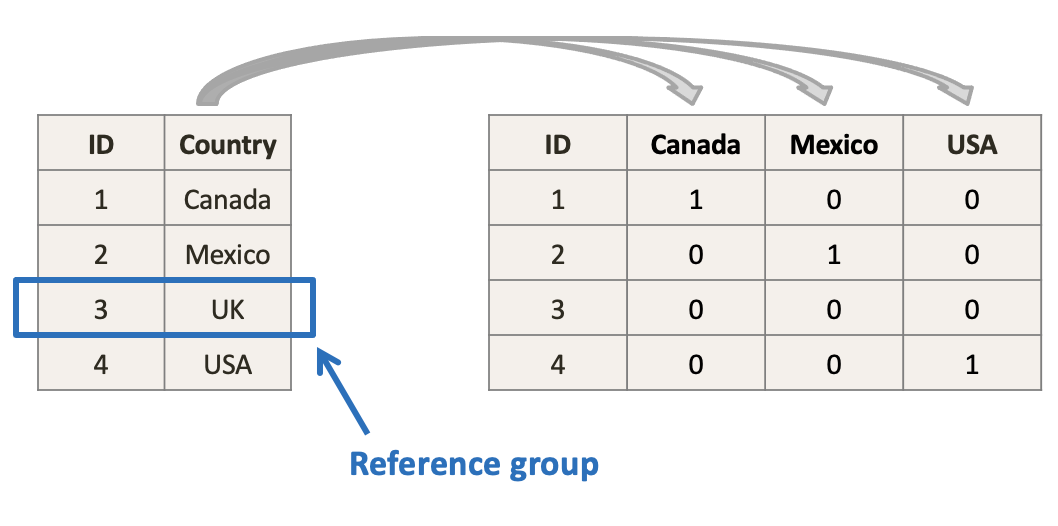
\includegraphics[width=0.75\linewidth]{/Users/craig.starbuck/Library/Mobile Documents/com~apple~CloudDocs/Documents/People Analytics Book/GitHub/peopleanalytics_lifecycle_book/graphics/onehot_encoding} 

}

\caption{One-Hot Encoding}\label{fig:onehot-encoding}
\end{figure}

For a categorical variable with only two values, the \texttt{ifelse()} function can be leveraged to assign values:

\begin{Shaded}
\begin{Highlighting}[]
\CommentTok{\# Return unique values of gender field}
\FunctionTok{unique}\NormalTok{(employees}\SpecialCharTok{$}\NormalTok{gender)}
\end{Highlighting}
\end{Shaded}

\begin{verbatim}
## [1] "Female" "Male"
\end{verbatim}

\begin{Shaded}
\begin{Highlighting}[]
\CommentTok{\# Gender one{-}hot encoding}
\NormalTok{employees}\SpecialCharTok{$}\NormalTok{gender\_ohe }\OtherTok{\textless{}{-}} \FunctionTok{ifelse}\NormalTok{(employees}\SpecialCharTok{$}\NormalTok{gender }\SpecialCharTok{==} \StringTok{\textquotesingle{}Female\textquotesingle{}}\NormalTok{, }\DecValTok{1}\NormalTok{, }\DecValTok{0}\NormalTok{)}

\CommentTok{\# Preview records}
\FunctionTok{head}\NormalTok{(}\FunctionTok{subset}\NormalTok{(employees, }\AttributeTok{select =} \FunctionTok{c}\NormalTok{(employee\_id, gender\_ohe)))}
\end{Highlighting}
\end{Shaded}

\begin{verbatim}
##   employee_id gender_ohe
## 1        1001          1
## 2        1002          0
## 3        1003          0
## 4        1004          1
## 5        1005          0
## 6        1006          0
\end{verbatim}

For variables with more than 2 categories, we can leverage the \texttt{model.matrix()} function for one-hot encoding. Let's illustrate be encoding locations.

\begin{Shaded}
\begin{Highlighting}[]
\CommentTok{\# Return counts by department}
\NormalTok{employees }\SpecialCharTok{\%\textgreater{}\%} \FunctionTok{count}\NormalTok{(dept, }\AttributeTok{sort =} \ConstantTok{TRUE}\NormalTok{)}
\end{Highlighting}
\end{Shaded}

\begin{verbatim}
##                     dept   n
## 1 Research & Development 961
## 2                  Sales 446
## 3        Human Resources  63
\end{verbatim}

By default, the \texttt{model.matrix()} function will produce a matrix of 1/0 values for \(k-1\) categories. The first column in the matrix is an intercept column containing a value of 1 for each row to ensure linear independence, and the default behavior results in the first value of the factor being the omitted group. For more flexibility over which value is omitted, we can drop the intercept using \texttt{-1} in the first argument passed to \texttt{model.matrix()} and then choose the reference group for the analysis in a subsequent step.

\begin{Shaded}
\begin{Highlighting}[]
\CommentTok{\# Department one{-}hot encoding}
\NormalTok{dept\_ohe }\OtherTok{\textless{}{-}} \FunctionTok{model.matrix}\NormalTok{(}\SpecialCharTok{\textasciitilde{}}\NormalTok{dept}\DecValTok{{-}1}\NormalTok{, }\AttributeTok{data =}\NormalTok{ employees)}

\CommentTok{\# Preview data}
\FunctionTok{head}\NormalTok{(dept\_ohe)}
\end{Highlighting}
\end{Shaded}

\begin{verbatim}
##   deptHuman Resources deptResearch & Development deptSales
## 1                   0                          0         1
## 2                   0                          1         0
## 3                   0                          1         0
## 4                   0                          1         0
## 5                   0                          1         0
## 6                   0                          1         0
\end{verbatim}

We will drop the department with the lowest \(n\) rather than the more arbitrary method based on the first value of the factor. Since departments are coded as either \(1\) or \(0\), we can use the \texttt{colSums()} function to sum each column and the \texttt{which.min()} function to identify which has the lowest sum (i.e., smallest department by employee count).

\begin{Shaded}
\begin{Highlighting}[]
\CommentTok{\# Drop department with lowest sum (lowest n{-}count)}
\NormalTok{dept\_ohe }\OtherTok{\textless{}{-}}\NormalTok{ dept\_ohe[, }\SpecialCharTok{{-}}\FunctionTok{which.min}\NormalTok{(}\FunctionTok{colSums}\NormalTok{(dept\_ohe))]}

\CommentTok{\# Preview refined one{-}hot encoded data}
\FunctionTok{head}\NormalTok{(dept\_ohe)}
\end{Highlighting}
\end{Shaded}

\begin{verbatim}
##   deptResearch & Development deptSales
## 1                          0         1
## 2                          1         0
## 3                          1         0
## 4                          1         0
## 5                          1         0
## 6                          1         0
\end{verbatim}

\begin{Shaded}
\begin{Highlighting}[]
\CommentTok{\# Combine employees and matrix containing one{-}hot encoded departments}
\NormalTok{employees }\OtherTok{\textless{}{-}} \FunctionTok{cbind}\NormalTok{(employees, dept\_ohe)}

\CommentTok{\# Drop original department field}
\NormalTok{employees }\OtherTok{\textless{}{-}} \FunctionTok{subset}\NormalTok{(employees, }\AttributeTok{select =} \SpecialCharTok{{-}}\FunctionTok{c}\NormalTok{(dept))}
\end{Highlighting}
\end{Shaded}

\hypertarget{feature-engineering}{%
\section{Feature Engineering}\label{feature-engineering}}

Level one people analytics tends to utilize only the delivered fields from the HRIS (e.g., location, job profile, org tenure), but a good next step is to derive smarter variables from these fields. These can then be used to cut data differently or as inputs in models. Below are some examples of how basic data available in the HRIS can be transformed into new variables that provide different information. This can be easily accomplished using the arithmetic functions we've covered.

\begin{itemize}
\tightlist
\item
  Number of jobs per unit of tenure (larger proportions tend to see greater career pathing)
\item
  Office/remote worker (binary variable dummy coded as 1/0)
\item
  Local/remote manager (binary variable dummy coded as 1/0)
\item
  Hire/Rehire (binary variable dummy coded as 1/0)
\item
  Hired/acquired (proxy for culture shock effects)
\item
  Gender isolation (ratio of employee's gender to number of the same within immediate work
  group)
\item
  Generation isolation (comparison of age bracket to most frequent generational bracket within
  immediate work group)
\item
  Ethnic isolation (ratio of employee's ethnicity to number of the same within immediate work
  group)
\item
  Difference between employee and manager age
\item
  Percentage change between last two performance appraisal scores (per competency and/or
  overall)
\item
  Team and department quit outbreak indicators (ratio of terms over x months relative to average
  headcount over x months)
\item
  Industry experience (binary or length in years)
\end{itemize}

\hypertarget{review-questions-6}{%
\section{Review Questions}\label{review-questions-6}}

\begin{enumerate}
\def\labelenumi{\arabic{enumi}.}
\item
  What are the differences between data lakes, data warehouses, and data marts?
\item
  What is the difference between a Type 1 and Type 2 table in a DW?
\item
  In what ways has modern cloud computing influenced data architecture?
\item
  Why is it dangerous to address missing values without domain knowledge of how the data are generated?
\item
  How can missing values be addressed when impacted records cannot be eliminated from a data set?
\item
  When is one-hot encoding required for categorical variables?
\item
  When one-hot encoding a categorical variable with more than two categories, why is an omitted category important?
\item
  When binning numeric data, what are some considerations in determining the size of each bin?
\item
  Why should variables with low to no variability be dropped?
\item
  Where are validation rules ideally situated to limit downstream data cleaning tasks and ensure consistent categorical dimension values?
\end{enumerate}

\hypertarget{aod}{%
\chapter{Analysis of Differences}\label{aod}}

There are many statistical tests that can be used to test for differences within or between two or more groups. This chapter will cover common contexts for differences in people analytics and the tests applicable to each.

\hypertarget{parametric-vs.-nonparametric-tests}{%
\section{Parametric vs.~Nonparametric Tests}\label{parametric-vs.-nonparametric-tests}}

In the context of data measured on a continuous scale (quantitative), we will cover parametric tests along with their nonparametric counterparts. When the hypothesis relates to average (mean) differences and \(n\) is large, \textbf{parametric tests} are preferred as they generally have more statistical power. \textbf{Nonparametric tests} are \textbf{distribution-free tests} that do not require the population's distribution to be characterized by certain parameters, such as a normal distribution defined by a mean and standard deviation. Nonparametric tests are great for qualitative data since the distribution of non-numeric data cannot be characterized by parameters.

Beyond ensuring the data were generated from a random and representative process as discussed in Chapter \ref{measure-sampl}, as well as following the data screening procedures outlined in Chapter \ref{data-mgmt-prep} (e.g., addressing concerning outliers), parametric tests of differences \emph{generally} feature three key assumptions:

\begin{enumerate}
\def\labelenumi{\arabic{enumi}.}
\tightlist
\item
  \textbf{Independence}: Observations within each group are independent of each other
\item
  \textbf{Homogeneity of Variance}: Variances of populations from which samples were drawn are equal
\item
  \textbf{Normality}: Residuals must be normally distributed (with mean of 0) within each group
\end{enumerate}

While homogeneity of variance assumes the variances across multiple groups are equal, parametric tests are generally robust to violations of equal variances when the sample sizes are large. Also, you may recall that \(\mu\) and \(\sigma\) are sufficient to characterize a population distribution when data are situated symmetrically around the mean. However, the mean can be sensitive to outliers so if outliers are present in the data, the median may be a better way of representing the data's center (i.e., nonparametric tests); just remember that the use of nonparametric tests requires hypotheses to be modified to adjust for \emph{median} -- rather than \emph{mean} -- centers.

You may be wondering whether the magical elixir that is the CLT, which we covered in Chapter \ref{inf-stats}, influences our ability to utilize parametric tests with respect to the assumption of normality. It's important to remember that the normal distribution properties under the CLT relate to the \emph{sampling distribution of means} -- not to the distribution of the population or to the data for an individual sample. The CLT is important for estimating population parameters, but it does not transform a population distribution from nonnormal to normal. If we know the population distribution is nonnormal (e.g., ordinal, nominal, or skewed data), nonparametric tests should be considered. This is why we used Spearman's correlation coefficient -- a nonparametric test -- in Chapter \ref{desc-stats} to evaluate the relationship between job level and education; these ordinal data are not normally distributed in the population.

\begin{Shaded}
\begin{Highlighting}[]
\CommentTok{\# Load employee data}
\NormalTok{employees }\OtherTok{\textless{}{-}} \FunctionTok{read.csv}\NormalTok{(}\StringTok{"/Users/craig.starbuck/Library/Mobile Documents/com\textasciitilde{}apple\textasciitilde{}CloudDocs/Documents/People Analytics Book/GitHub/peopleanalytics\_lifecycle\_book/data/employees.csv"}\NormalTok{)}
\end{Highlighting}
\end{Shaded}

\hypertarget{differences-in-discrete-data}{%
\section{Differences in Discrete Data}\label{differences-in-discrete-data}}

Nonparametric tests are generally best when working with data measured on a discrete scale since these data do not come from normally distributed populations. The two most commonly used tests to analyze variables measured on a discrete scale are the nonparametric \emph{Chi-square test} and \emph{Fisher's exact test}.

\begin{figure}

{\centering 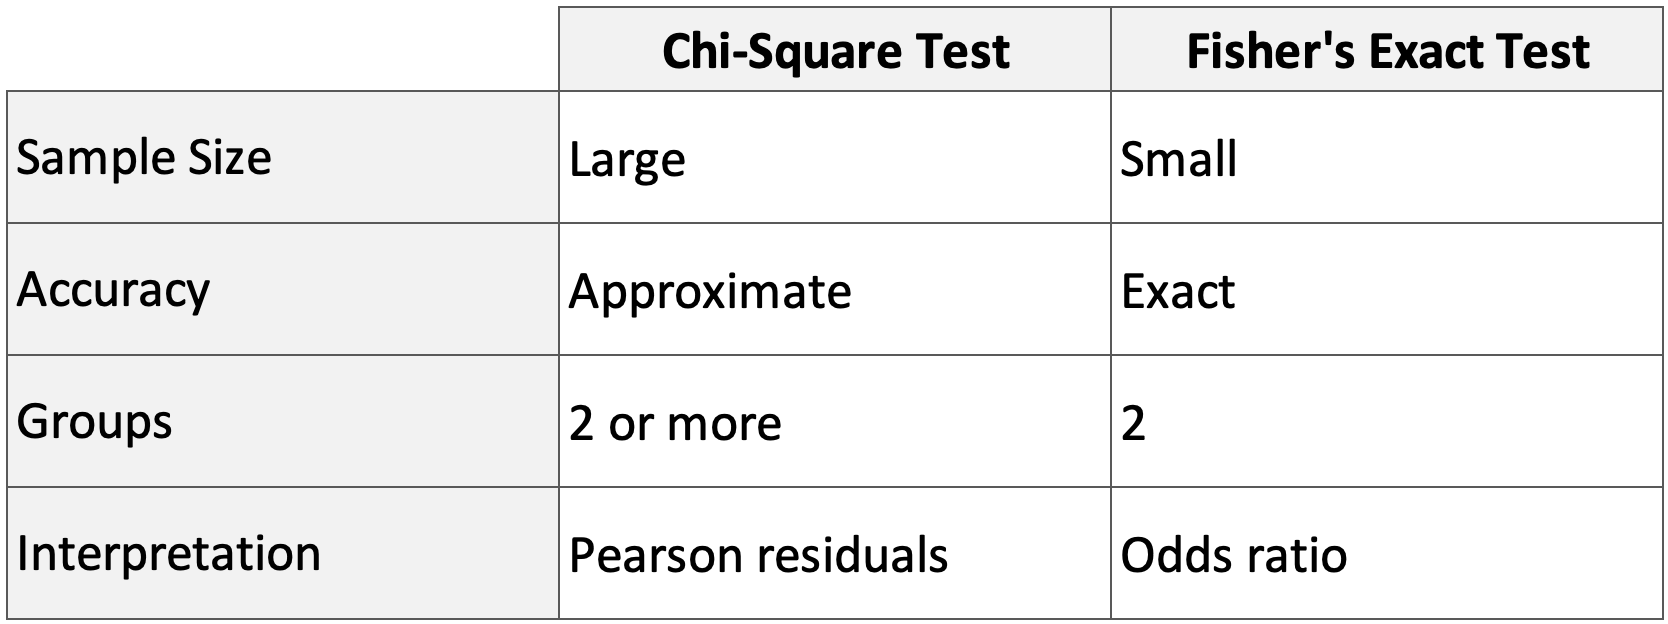
\includegraphics[width=1\linewidth]{/Users/craig.starbuck/Library/Mobile Documents/com~apple~CloudDocs/Documents/People Analytics Book/GitHub/peopleanalytics_lifecycle_book/graphics/discrete_differences_test_table} 

}

\caption{Chi-Square and Fisher Exact Test Criteria for Discrete Data}\label{fig:discrete-tests}
\end{figure}

Both tests organize data within 2x2 \textbf{contingency tables} which enables us to understand interrelations between variables.

\textbf{Chi-Square Test}

The \textbf{Chi-Square Test of Independence} evaluates patterns of observations to determine if categories occur more frequently than we would expect by chance. The Chi-square statistic is defined by:

\[ {\chi}^2 = \sum\frac{(O_i - E_i)^2}{E_i}, \]

where \(O_i\) is the observed value, and \(E_i\) is the expected value.

\(H_0\) states that each variable is independent of one another (i.e., there is no relationship). In addition to the \({\chi}^2\) test statistic, \(df\) for the contingency table, defined by \(df = (rows - 1) * (columns - 1)\), is required to determine whether we reject or fail to reject \(H_0\).

While there is not consensus on the minimum sample size for this test, it is important to note that the \({\chi}^2\) statistic follows a chi-square distribution \emph{asymptotically}. This means we can only calculate accurate \(p\)-values for larger samples, and a general rule of thumb is that the expected value for each cell needs to be at least 5. The challenge with small \(n\)-counts is illustrated in Figure \ref{fig:chisq-dist}; the chi-square distribution approaches a vertical line as \(df\) drops below 5.

\begin{figure}

{\centering 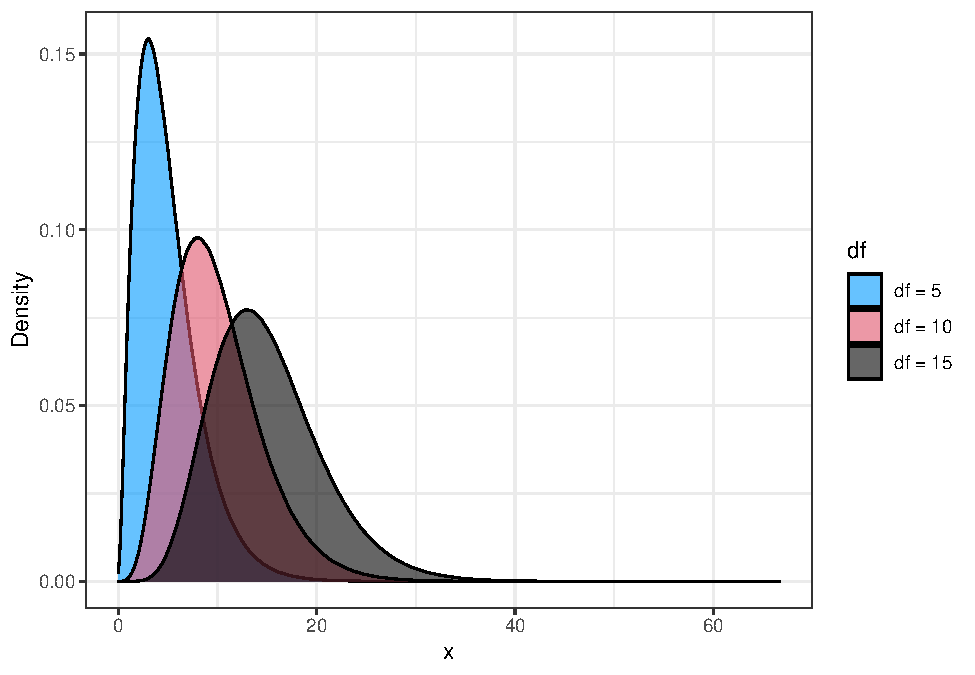
\includegraphics[width=1\linewidth]{People_Analytics_Lifecycle_files/figure-latex/chisq-dist-1} 

}

\caption{Chi-Square Distributions by Degrees of Freedom (df)}\label{fig:chisq-dist}
\end{figure}

We will demonstrate how to perform a chi-square test of independence by evaluating whether exit rates are independent of whether an employee works overtime. Let's first construct a 2x2 contingency table using the \texttt{table()} function:

\begin{Shaded}
\begin{Highlighting}[]
\CommentTok{\# Create contingency table}
\NormalTok{cont\_tbl }\OtherTok{\textless{}{-}} \FunctionTok{table}\NormalTok{(employees}\SpecialCharTok{$}\NormalTok{active, employees}\SpecialCharTok{$}\NormalTok{overtime)}
\NormalTok{cont\_tbl}
\end{Highlighting}
\end{Shaded}

\begin{verbatim}
##      
##        No Yes
##   No  110 127
##   Yes 944 289
\end{verbatim}

A \textbf{mosaic plot} is a great way to visualize the delta between expected and observed frequencies for each cell. This can be produced using the \texttt{mosaicplot()} function from the \texttt{graphics} library:

\begin{figure}

{\centering 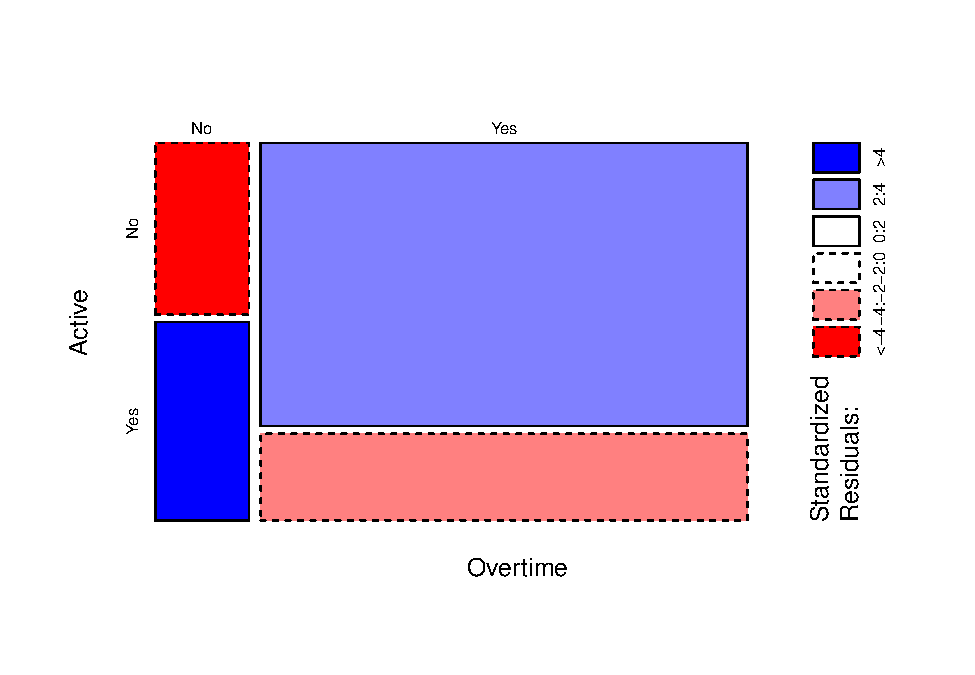
\includegraphics[width=1\linewidth]{People_Analytics_Lifecycle_files/figure-latex/mosaic-plot-1} 

}

\caption{Mosaic Plot of Residuals for Overtime x Active Status}\label{fig:mosaic-plot}
\end{figure}

In Figure \ref{fig:mosaic-plot}, blue indicates that the observed value is higher than the expected value, while red indicates that the observed value is lower than the expected value. Based on this plot, there appears to be some meaningful patterns and departures from expected values in both the high and low directions. There are more inactive employees than expected in the overtime group, and more active employees than expected in the group with no overtime. These large standardized residuals are indicative of meaningful relationships between the two categorical variables.

Let's run the chi-square test of independence to determine whether these residuals are statistically significant. This test can be performed in R by passing the contingency table into the \texttt{chisq.test()} function:

\begin{Shaded}
\begin{Highlighting}[]
\CommentTok{\# Perform chi{-}square test of independence}
\FunctionTok{chisq.test}\NormalTok{(cont\_tbl)}
\end{Highlighting}
\end{Shaded}

\begin{verbatim}
## 
##  Pearson's Chi-squared test with Yates' continuity correction
## 
## data:  cont_tbl
## X-squared = 87.564, df = 1, p-value < 2.2e-16
\end{verbatim}

Based on the results, exit rates are not independent of overtime (\({\chi}^2(1) = 87.56, p < .05\)). Therefore, there is a statistically significant relationship between an employee working overtime and the rate at which they change from an active to inactive status -- confirming what was evident in the mosaic plot.

\textbf{Fisher's Exact Test}

When the sample size is small, \textbf{Fisher's Exact Test} can be used to calculate the \emph{exact} \(p\)-value rather than an approximation, which is the case with many statistical tests such as the chi-square test.

\(H_0\) for Fisher's exact test is the same as \(H_0\) for the chi-square test of independence: There is no relationship between the two categorical variables (i.e., they are independent). We can perform Fisher's exact test using the \texttt{fisher.test()} function in R:

\begin{Shaded}
\begin{Highlighting}[]
\CommentTok{\# Perform Fisher\textquotesingle{}s exact test}
\FunctionTok{fisher.test}\NormalTok{(cont\_tbl)}
\end{Highlighting}
\end{Shaded}

\begin{verbatim}
## 
##  Fisher's Exact Test for Count Data
## 
## data:  cont_tbl
## p-value < 2.2e-16
## alternative hypothesis: true odds ratio is not equal to 1
## 95 percent confidence interval:
##  0.1969101 0.3572582
## sample estimates:
## odds ratio 
##  0.2654384
\end{verbatim}

Note the \emph{odds ratio} shown in this output. The \textbf{odds ratio} represents the ratio of positive to negative cases, which is the ratio of overtime for active and inactive workers in this example. The odds ratio is defined by:

\[OR = \frac{a*d}{b*c}\]

An odds ratio of 1 indicates no difference in overtime frequency between active and inactive workers. Figure \ref{fig:contingency-tbl} illustrates the cells for the odds ratio calculation for the 2x2 contingency table of overtime for active and inactive (termed) workers.

\begin{figure}

{\centering 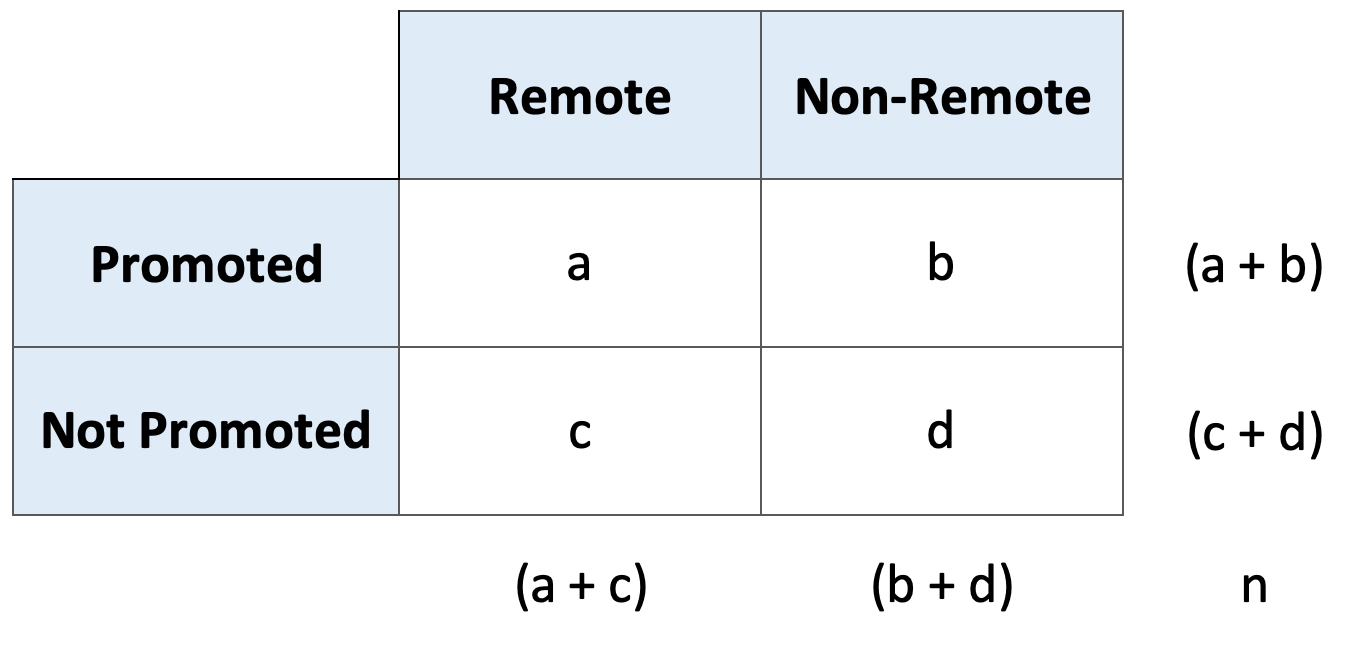
\includegraphics[width=0.75\linewidth]{/Users/craig.starbuck/Library/Mobile Documents/com~apple~CloudDocs/Documents/People Analytics Book/GitHub/peopleanalytics_lifecycle_book/graphics/contingency_table} 

}

\caption{2x2 Contingency Table of Overtime for Active and Inactive Workers}\label{fig:contingency-tbl}
\end{figure}

Since the 95\% \(CI\) for the odds ratio does not include 1, we reject the null hypothesis and conclude that exit rates are related to working overtime; this is consistent with results from the chi-square test of independence. Since overtime was indicated far more often for inactive workers than for active workers, it is no surprise that the denominator of our ratio is larger than the numerator (i.e., \(OR\) \textless{} 1).

As discussed in Chapter \ref{desc-stats}, we can produce a \(\phi\) coefficient to understand the strength of the association by passing the contingency table into the \texttt{phi} function from the \texttt{psych} library:

\begin{Shaded}
\begin{Highlighting}[]
\CommentTok{\# Calculate the Phi Coefficient}
\NormalTok{psych}\SpecialCharTok{::}\FunctionTok{phi}\NormalTok{(cont\_tbl)}
\end{Highlighting}
\end{Shaded}

\begin{verbatim}
## [1] -0.25
\end{verbatim}

The relationship between active status and overtime is negative, and the strength of the relationship is weak (\(\phi\) = -.25).

Another common method of measuring the strength of the association between two categorical variables is \textbf{Cramer's V}, which ranges from 0 (no association) to 1 (strong association). In the interest of not muddying the waters with an exhaustive set of alernative methods, the implementation won't be covered.

\hypertarget{differences-in-continuous-data}{%
\section{Differences in Continuous Data}\label{differences-in-continuous-data}}

A variety of parametric and nonparametric tests are available for evaluating differences between variables measured on a continuous scale. Figure \ref{fig:continuous-tests} provides a side-by-side of these parametric and corresponding nonparametric tests of differences.

\begin{figure}

{\centering 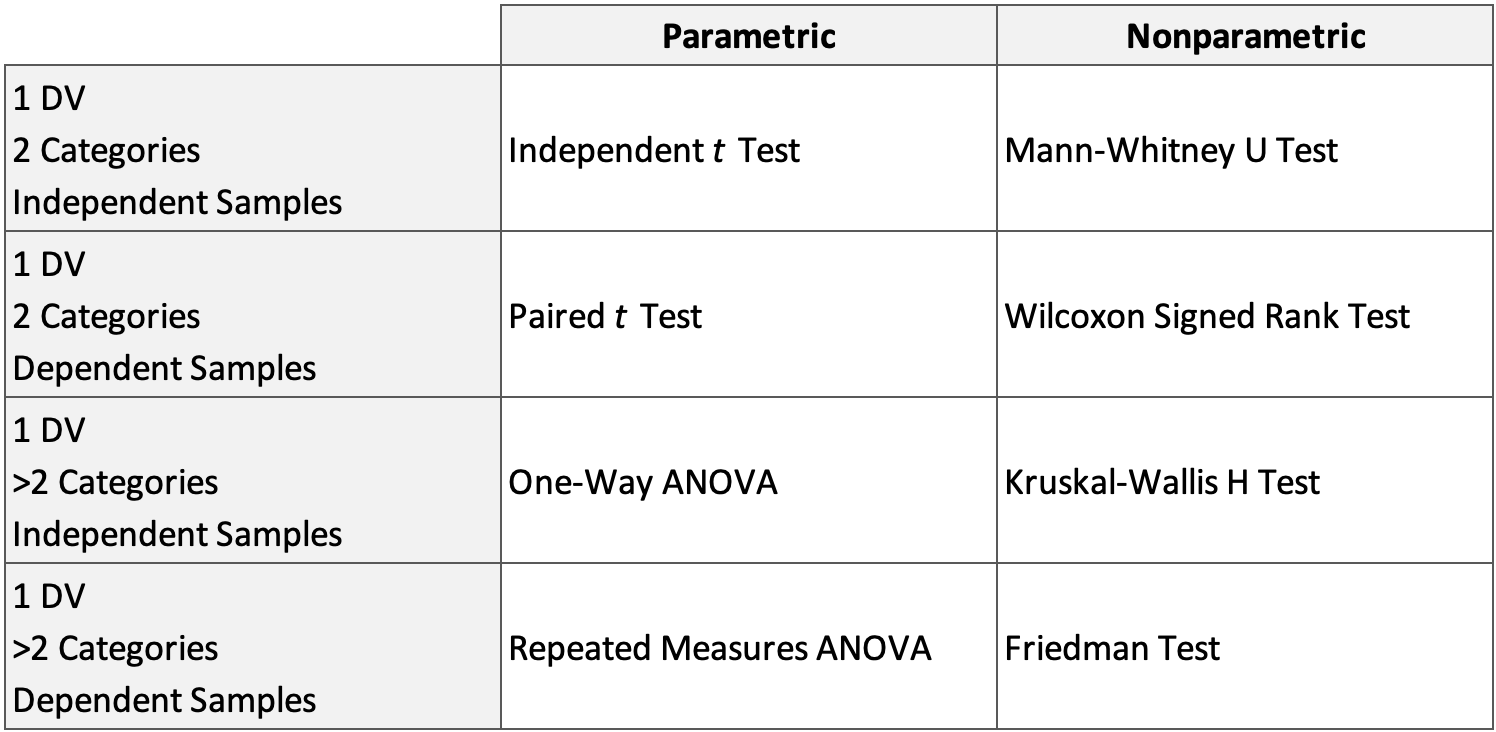
\includegraphics[width=1\linewidth]{/Users/craig.starbuck/Library/Mobile Documents/com~apple~CloudDocs/Documents/People Analytics Book/GitHub/peopleanalytics_lifecycle_book/graphics/continuous_differences_test_table} 

}

\caption{Parametric and Nonparametric Tests of Differences for Continuous Data}\label{fig:continuous-tests}
\end{figure}

\textbf{Independent Samples }\(\textbf t\)\textbf{-Test}

When evaluating differences between two independent samples, social psychology researchers generally select from two tests: \emph{Student's} \(t\)\emph{-test} and \emph{Welch's} \(t\)\emph{-test}. There are other alternatives, such as \emph{Yuen's} \(t\)\emph{-test} and a \emph{bootstrapped} \(t\)\emph{-test}, but these are less commonly reported in scholarly social science journals and will not be covered in this book.

The \textbf{Student's} \(t\)\textbf{-test}, which was introduced in Chapter \ref{inf-stats}, is a parametric test whose assumptions of equal variances seldom hold in people analytics. \textbf{Welch's} \(t\)\textbf{-test} is generally preferred to the Student's \(t\)-test because it has been shown to provide better control of Type 1 error rates when homogeneity of variance is not met, whilst losing little robustness (e.g., Delacre, Lakens, \& Leys, 2017). When \(n\) is equal between groups, the Student's \(t\)-test is known to be robust to violations of the equal variance assumption, as long as \(n\) is sufficiently high to accurately estimate parameters and the underlying distribution is not characterized by high skewness and kurtosis.

Let's explore the mechanics of independent samples \(t\)-tests. Figure \ref{fig:mean-group-diff} illustrates mean differences (\(MD\)) for nine Welch's \(t\)-tests based on random sample data generated from independent normal populations. Remember that statistical power increases with a large \(n\), as \(t\) distributions approximate a standard normal distribution with larger \(df\). In the context of analysis of differences, this translates to an increase in the likelihood of detecting statistical differences in the means of two distributions. Note that for the two cases where both \(MD\) and \(n\) are relatively small, mean differences are not statistically significant (\(p > .05\)). You may also notice that as the \(t\)-statistic approaches 0, statistical differences become less likely since a smaller \(t\)-statistic indicates a smaller difference between mean values.

\begin{figure}

{\centering 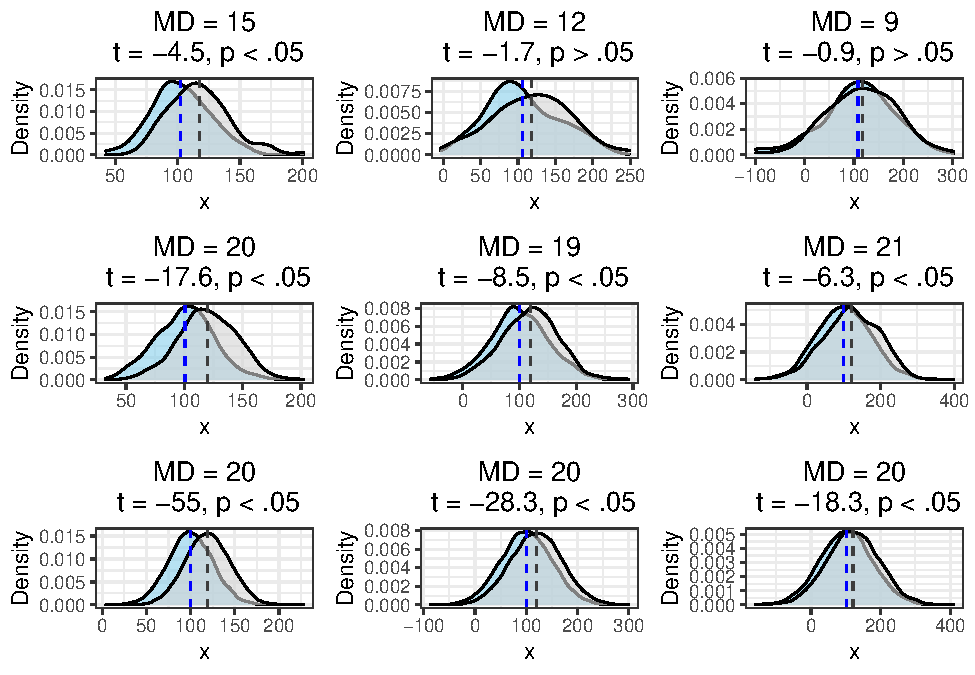
\includegraphics[width=1\linewidth]{People_Analytics_Lifecycle_files/figure-latex/mean-group-diff-1} 

}

\caption{Density plots comparing distributions with a mean of 100 (blue) and 120 (grey) with sample sizes of 100, 1,000, and 10,000 (rows) and standard deviations of 25, 50, and 75 (columns). Dashed vertical lines represent distribution means.}\label{fig:mean-group-diff}
\end{figure}

Next, we will walk through the steps involved in performing Welch's \(t\)-test. Let's first visualize the distribution of data for each group using boxplots:

\begin{figure}

{\centering 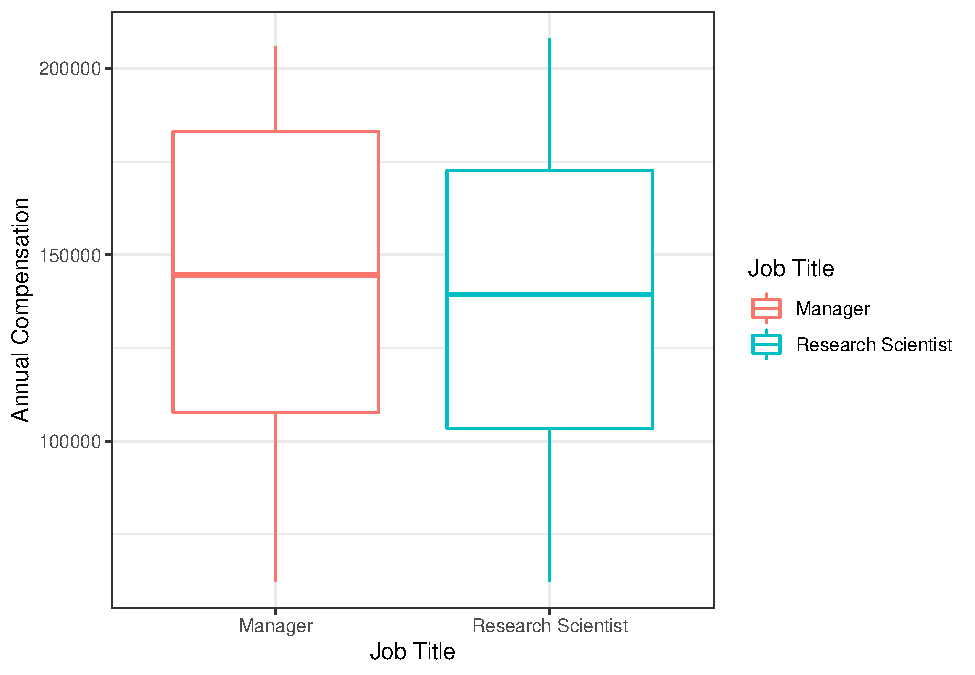
\includegraphics[width=1\linewidth]{People_Analytics_Lifecycle_files/figure-latex/comp-job-boxplots-1} 

}

\caption{Annual Compensation Distributions for Managers and Research Scientists}\label{fig:comp-job-boxplots}
\end{figure}

While the median -- rather than the mean which is being evaluated with Welch's \(t\)-test -- is shown in these boxplots, this is a great way to visually inspect whether there are meaningful differences in the distribution of data between groups (in addition to identifying outliers). We could of course use density plots or histograms as an alternative. As we can see, annual compensation for employees with a Manager job title tends to be slightly higher than for those with a Research Scientist job title, and the variance in annual compensation appears to be fairly consistent between the groups.

There are several alternatives to a visual inspection of normality, such as the \({\chi}^2\) \textbf{Goodness-of-Fit test} (Snedecor \& Cochran, 1980), \textbf{Kolmogorov-Smirnov (K-S) test} (Chakravarti, Laha, \& Roy, 1967), or \textbf{Shapiro-Wilk test} (Shapiro \& Wilk, 1965). The general idea is consistent for each of these tests: compare observed data to what would be expected if data are sampled from a normally distributed population. The \({\chi}^2\) Goodness-of-Fit test compares the \emph{count} of data points across the range of values relative to what would be expected in each for a sample with the same dimensions taken from a normal distribution. For example, if data are sampled from a normal population distribution, it follows that roughly half the values should exist below the mean and half above the mean. The K-S test evaluates how the observed \emph{cumulative} distribution compares to the properties of a normal \emph{cumulative} distribution. The Shapiro-Wilk test is based on \emph{correlations} between observed and expected data.

We will test for normality using the Shapiro-Wilk test. The null hypothesis for the Shapiro-Wilk test is that the data are normally distributed, so a high \(p\)-value indicates that the assumption of normality is satisfied (i.e., failure to reject the null hypothesis of normally distributed data). We can use the \texttt{with()} function together with the \texttt{shapiro.test()} function to run this test in R:

\begin{Shaded}
\begin{Highlighting}[]
\CommentTok{\# Compute Shapiro{-}Wilk test of normality for each group}
\FunctionTok{with}\NormalTok{(employees, }\FunctionTok{shapiro.test}\NormalTok{(annual\_comp[job\_title }\SpecialCharTok{==} \StringTok{\textquotesingle{}Manager\textquotesingle{}}\NormalTok{]))}
\end{Highlighting}
\end{Shaded}

\begin{verbatim}
## 
##  Shapiro-Wilk normality test
## 
## data:  annual_comp[job_title == "Manager"]
## W = 0.93546, p-value = 0.000103
\end{verbatim}

\begin{Shaded}
\begin{Highlighting}[]
\FunctionTok{with}\NormalTok{(employees, }\FunctionTok{shapiro.test}\NormalTok{(annual\_comp[job\_title }\SpecialCharTok{==} \StringTok{\textquotesingle{}Research Scientist\textquotesingle{}}\NormalTok{]))}
\end{Highlighting}
\end{Shaded}

\begin{verbatim}
## 
##  Shapiro-Wilk normality test
## 
## data:  annual_comp[job_title == "Research Scientist"]
## W = 0.96002, p-value = 3.427e-07
\end{verbatim}

Based on these tests, the distribution of annual compensation for Managers and Research Scientists are significantly different from normally distributed data (\(p\) \textless{} .05).

While we should not proceed with performing Welch's \(t\)-test due to unequal variances, let's do so merely to illustrate how the test is implemented in R. To perform Welch's \(t\)-test in R, we can simply pass into the \texttt{t.test()} function a numeric vector for each of the two groups.

\begin{Shaded}
\begin{Highlighting}[]
\CommentTok{\# Create compensation vectors for two jobs}
\NormalTok{comp\_mgr }\OtherTok{\textless{}{-}} \FunctionTok{unlist}\NormalTok{(}\FunctionTok{subset}\NormalTok{(employees, job\_title }\SpecialCharTok{==} \StringTok{\textquotesingle{}Manager\textquotesingle{}}\NormalTok{, }\AttributeTok{select =}\NormalTok{ annual\_comp))}
\NormalTok{comp\_rsci }\OtherTok{\textless{}{-}} \FunctionTok{unlist}\NormalTok{(}\FunctionTok{subset}\NormalTok{(employees, job\_title }\SpecialCharTok{==} \StringTok{\textquotesingle{}Research Scientist\textquotesingle{}}\NormalTok{, }\AttributeTok{select =}\NormalTok{ annual\_comp))}

\CommentTok{\# Run Welch\textquotesingle{}s t{-}test}
\FunctionTok{t.test}\NormalTok{(comp\_mgr, comp\_rsci)}
\end{Highlighting}
\end{Shaded}

\begin{verbatim}
## 
##  Welch Two Sample t-test
## 
## data:  comp_mgr and comp_rsci
## t = 0.22623, df = 159.55, p-value = 0.8213
## alternative hypothesis: true difference in means is not equal to 0
## 95 percent confidence interval:
##  -8860.685 11153.244
## sample estimates:
## mean of x mean of y 
##  139900.8  138754.5
\end{verbatim}

If the data adhered to the assumptions of Welch's \(t\)-test, we would conclude that the mean difference between annual compensation for Managers (\(\bar{x}\) = 139,901) and Research Scientists (\(\bar{x}\) = 138,755) is not significant (\(t(159.55)\) = .23, \(p\) = .82).

Note that we can access specific metrics from this output by storing results to an object and then referencing specific elements by name or index:

\begin{Shaded}
\begin{Highlighting}[]
\CommentTok{\# This assigns each element of results from Welch\textquotesingle{}s t{-}test to an indexed position in the object}
\NormalTok{t\_rslts }\OtherTok{\textless{}{-}} \FunctionTok{t.test}\NormalTok{(comp\_mgr, comp\_rsci)}

\NormalTok{t\_rslts}\SpecialCharTok{$}\NormalTok{statistic }\CommentTok{\# t{-}statistic}
\end{Highlighting}
\end{Shaded}

\begin{verbatim}
##         t 
## 0.2262262
\end{verbatim}

\begin{Shaded}
\begin{Highlighting}[]
\NormalTok{t\_rslts}\SpecialCharTok{$}\NormalTok{parameter }\CommentTok{\# df}
\end{Highlighting}
\end{Shaded}

\begin{verbatim}
##       df 
## 159.5544
\end{verbatim}

\begin{Shaded}
\begin{Highlighting}[]
\NormalTok{t\_rslts}\SpecialCharTok{$}\NormalTok{p.value }\CommentTok{\# p{-}value}
\end{Highlighting}
\end{Shaded}

\begin{verbatim}
## [1] 0.8213151
\end{verbatim}

\begin{Shaded}
\begin{Highlighting}[]
\NormalTok{t\_rslts}\SpecialCharTok{$}\NormalTok{method }\CommentTok{\# type of t{-}test}
\end{Highlighting}
\end{Shaded}

\begin{verbatim}
## [1] "Welch Two Sample t-test"
\end{verbatim}

When object elements are referenced by index, the element name is displayed in the output to clarify what the metric represents:

\begin{Shaded}
\begin{Highlighting}[]
\NormalTok{t\_rslts[}\DecValTok{1}\NormalTok{] }\CommentTok{\# t{-}statistic}
\end{Highlighting}
\end{Shaded}

\begin{verbatim}
## $statistic
##         t 
## 0.2262262
\end{verbatim}

\begin{Shaded}
\begin{Highlighting}[]
\NormalTok{t\_rslts[}\DecValTok{2}\NormalTok{] }\CommentTok{\# df}
\end{Highlighting}
\end{Shaded}

\begin{verbatim}
## $parameter
##       df 
## 159.5544
\end{verbatim}

\begin{Shaded}
\begin{Highlighting}[]
\NormalTok{t\_rslts[}\DecValTok{3}\NormalTok{] }\CommentTok{\# p{-}value}
\end{Highlighting}
\end{Shaded}

\begin{verbatim}
## $p.value
## [1] 0.8213151
\end{verbatim}

\begin{Shaded}
\begin{Highlighting}[]
\NormalTok{t\_rslts[}\DecValTok{9}\NormalTok{] }\CommentTok{\# type of t{-}test}
\end{Highlighting}
\end{Shaded}

\begin{verbatim}
## $method
## [1] "Welch Two Sample t-test"
\end{verbatim}

Given \(df\) = 159.55, you may be wondering how \(df\) is calculated for Welch's \(t\)-test given that thus far, we have only discussed the basic \(df\) calculation outlined in Chapter \ref{inf-stats}; namely, \(df = n - 1\). Welch's \(t\)-test uses the \textbf{Welch-Satterthwaite equation} for \(df\) (Satterthwaite, 1946; Welch, 1947). This equation approximates \(df\) for a linear combination of independent sample variances; which means that if samples are not independent, this approximation may not be valid. The Welch-Satterthwaite equation is defined by:

\[ df = \frac {(\frac{s^2_1}{n_1} + \frac{s^2_2}{n_2})^2} {\frac{1}{n_1 - 1} (\frac{s^2_1}{n_1})^2 + \frac{1}{n_2 - 1} (\frac{s^2_2}{n_2})^2} \]

\textbf{Cohen's} \(\textbf d\) is a standardized measure of the difference between two means that helps us understand the size (or \emph{practical} significance) of observed mean differences. Cohen's \(d\) is defined by:

\[ d = \frac{\bar{x}_1 - \bar{x}_2} {s_p},  \]

where \(s_p\) represents the pooled standard deviation defined by:

\[ s_p = \sqrt\frac{s^2_1 + s^2_2}{2} \]

Cohen's \(d\) can be produced using the \texttt{cohen.d()} function from the \texttt{effsize} package in R. The following thresholds can be referenced as a \emph{general} rule of thumb for interpreting effect size:

\begin{itemize}
\tightlist
\item
  \textbf{Small} = 0.2
\item
  \textbf{Medium} = 0.5
\item
  \textbf{Large} = 0.8
\end{itemize}

\begin{Shaded}
\begin{Highlighting}[]
\CommentTok{\# Load library for effect size functions}
\FunctionTok{library}\NormalTok{(effsize)}

\CommentTok{\# Perform Cohen\textquotesingle{}s d}
\NormalTok{effsize}\SpecialCharTok{::}\FunctionTok{cohen.d}\NormalTok{(comp\_mgr, comp\_rsci)}
\end{Highlighting}
\end{Shaded}

\begin{verbatim}
## 
## Cohen's d
## 
## d estimate: 0.0273669 (negligible)
## 95 percent confidence interval:
##      lower      upper 
## -0.2004390  0.2551728
\end{verbatim}

Not only are the differences statistically insignificant, Cohen's \(d\) = .03 indicates a negligible difference. Therefore, there is nothing of interest based on these statistical and practical significance tests.

\textbf{Mann-Whitney U Test}

A popular nonparametric (distribution-free) alternative to Welch's \(t\)-test is the \textbf{Mann-Whitney U Test}, also referred to as the \textbf{Wilcoxon Rank-Sum Test}. Rather than comparing the mean between two groups, like the Student's \(t\)-test or Welch's \(t\)-test, the Mann-Whitney U test considers the entire distribution by evaluating the extent to which the \emph{ranks} are consistent between groups (i.e., similarity in the proportion of records with each value). When distributions are similar, the medians of the two groups are compared.

The \texttt{wilcox.test()} function is used to run this test in R. Let's illustrate by examining whether engagement (an ordinal variable in our dataset) is significantly different between those who have been promoted in the past year and those who have not:

\begin{Shaded}
\begin{Highlighting}[]
\CommentTok{\# Create dummy{-}coded promotion variable}
\NormalTok{employees}\SpecialCharTok{$}\NormalTok{promo }\OtherTok{\textless{}{-}} \FunctionTok{ifelse}\NormalTok{(employees}\SpecialCharTok{$}\NormalTok{last\_promo }\SpecialCharTok{==} \DecValTok{1}\NormalTok{, }\DecValTok{1}\NormalTok{, }\DecValTok{0}\NormalTok{)}

\CommentTok{\# Create numeric engagement vectors for promo groups}
\NormalTok{no\_promo }\OtherTok{\textless{}{-}} \FunctionTok{unlist}\NormalTok{(}\FunctionTok{subset}\NormalTok{(employees, promo }\SpecialCharTok{==} \DecValTok{0}\NormalTok{, }\AttributeTok{select =}\NormalTok{ engagement))}
\NormalTok{promo }\OtherTok{\textless{}{-}} \FunctionTok{unlist}\NormalTok{(}\FunctionTok{subset}\NormalTok{(employees, promo }\SpecialCharTok{==} \DecValTok{1}\NormalTok{, }\AttributeTok{select =}\NormalTok{ engagement))}

\CommentTok{\# Perform the Mann{-}Whitney U (aka Wilcoxon rank{-}sum) test}
\FunctionTok{wilcox.test}\NormalTok{(no\_promo, promo)}
\end{Highlighting}
\end{Shaded}

\begin{verbatim}
## 
##  Wilcoxon rank sum test with continuity correction
## 
## data:  no_promo and promo
## W = 196056, p-value = 0.6707
## alternative hypothesis: true location shift is not equal to 0
\end{verbatim}

Based on these results, we fail to reject the null hypothesis, which states that there is no difference in engagement between those with and without promotions (\(W\) = 196,056, \(p\) = .67). Note the reference to continuity correction in the output. \textbf{Continuity correction} is applied when using a continuous distribution to approximate a discrete distribution. The Mann-Whitney U test we performed approximated a continuous distribution for testing differences between our ordinal (discrete) engagement data by applying this continuity correction.

Just as Cohen's \(d\) is used to measure the magnitude of difference between a pair of means, \textbf{Cliff's delta} can be leveraged to evaluate the size of differences between ordinal variables. Cliff's delta measures how often a value in one distribution is higher than values in another, and this is appropriate in situations in which a nonparametric test of differences is used. This statistic can be produced using the \texttt{cliff.delta()} function from the \texttt{effsize} package in R.

\begin{Shaded}
\begin{Highlighting}[]
\CommentTok{\# Run Cliff\textquotesingle{}s Delta}
\NormalTok{effsize}\SpecialCharTok{::}\FunctionTok{cliff.delta}\NormalTok{(no\_promo, promo)}
\end{Highlighting}
\end{Shaded}

\begin{verbatim}
## 
## Cliff's Delta
## 
## delta estimate: -0.0131625 (negligible)
## 95 percent confidence interval:
##       lower       upper 
## -0.07329491  0.04706528
\end{verbatim}

Some (e.g., Vargha \& Delaney, 2000) have endeavored to categorize the Cliff's delta statistic, which ranges from -1 to 1, into effect size buckets. However, such categorizations are far more controversial than thresholds attributed to Cohen's \(d\). Nevertheless, the near-zero delta estimate of -.01 indicates a negligible difference.

\textbf{Paired Samples} \(\textbf t\)\textbf{-Test}

A \textbf{Paired Samples }\(\textbf t\)\textbf{-Test} is used to compare means between pairs of measurements. This test is known by many other names, such as a \textbf{dependent samples} \(\textbf t\)\textbf{-test}, \textbf{paired-difference} \(\textbf t\)\textbf{-test}, \textbf{matched pairs} \(\textbf t\)\textbf{-test}, and \textbf{repeated-samples} \(\textbf t\)\textbf{-test}.

The assumption of normality in the context of a paired samples \(t\)-test relates to normally distributed paired differences. This is important, as the \(p\)-value for the test statistic will not be valid if this assumption is violated.

To illustrate, let's design an experiment. Let's assume morale has declined for employees who travel frequently, and several actions have been proposed by a task force to help address this. The task force has decided to pilot a new flexible work benefit over a six-month period to determine if it has a meaningful effect on morale. This new benefit is piloted to a random sample of frequent travelers, and our task is to test whether the outcomes warrant a broader rollout to frequent travelers.

Our DV (happiness) will be measured using a composite index derived from individual engagement, environment satisfaction, job satisfaction, and relationship satisfaction scores. Our objective is to determine if there is a significant improvement in this happiness index for the treatment group (those who are part of the flexible work pilot) relative to the pre/post difference for the control group (those not selected for the flexible work pilot).

While we could simply look at the pre/post differences for the treatment group, we understand from Chapter \ref{research} that this would be a weak design that may lead to inaccurate conclusions. There could be alternative explanations for any observed increases in happiness that are unrelated to the intervention itself. For example, between time 1 and time 2, travel frequency may have decreased for everyone, which may contribute to overall happiness. By comparing pre/post differences between the treatment and control groups, we gain more confidence in isolating the effect of the flexible work benefit on happiness since alternative explanations should be reflected in any pre/post changes observed for the control group.

\textbf{Difference-in-differences (DiD)} estimation is a quasi-experimental approach that originated from econometrics for this same purpose, but it is beyond the scope of this book. Angrist and Pischke (2009) is an excellent resource for learning about these methods.

Let's prepare the data for this experiment. Since \texttt{employees} is a cross-sectional dataset (single point-in-time), we will generate simulated data for repeated measures (i.e., post-intervention scores).

\begin{Shaded}
\begin{Highlighting}[]
\CommentTok{\# Set seed for reproducible results}
\FunctionTok{set.seed}\NormalTok{(}\DecValTok{1234}\NormalTok{)}

\CommentTok{\# Derive happiness index from survey variables}
\NormalTok{employees}\SpecialCharTok{$}\NormalTok{happiness\_ind }\OtherTok{\textless{}{-}}\NormalTok{ (employees}\SpecialCharTok{$}\NormalTok{engagement }\SpecialCharTok{+}\NormalTok{ employees}\SpecialCharTok{$}\NormalTok{env\_sat }\SpecialCharTok{+}\NormalTok{ employees}\SpecialCharTok{$}\NormalTok{job\_sat }\SpecialCharTok{+}\NormalTok{ employees}\SpecialCharTok{$}\NormalTok{rel\_sat) }\SpecialCharTok{/} \DecValTok{4}

\CommentTok{\# Sample size of frequent travelers}
\NormalTok{n }\OtherTok{=} \FunctionTok{nrow}\NormalTok{(}\FunctionTok{subset}\NormalTok{(employees, business\_travel }\SpecialCharTok{==} \StringTok{\textquotesingle{}Travel\_Frequently\textquotesingle{}}\NormalTok{, }\AttributeTok{select =}\NormalTok{ employee\_id))}

\CommentTok{\# Randomly assign half of frequent travelers to treatment and control groups}
\NormalTok{treat\_ids }\OtherTok{\textless{}{-}} \FunctionTok{sample}\NormalTok{(}\FunctionTok{unlist}\NormalTok{(}\FunctionTok{subset}\NormalTok{(employees, business\_travel }\SpecialCharTok{==} \StringTok{\textquotesingle{}Travel\_Frequently\textquotesingle{}}\NormalTok{, }\AttributeTok{select =}\NormalTok{ employee\_id)), }\FunctionTok{floor}\NormalTok{(n }\SpecialCharTok{*}\NormalTok{ .}\DecValTok{5}\NormalTok{))}
\NormalTok{ctrl\_ids }\OtherTok{\textless{}{-}} \FunctionTok{unlist}\NormalTok{(}\FunctionTok{subset}\NormalTok{(employees, business\_travel }\SpecialCharTok{==} \StringTok{\textquotesingle{}Travel\_Frequently\textquotesingle{}} \SpecialCharTok{\&} \SpecialCharTok{!}\NormalTok{employee\_id }\SpecialCharTok{\%in\%}\NormalTok{ treat\_ids, }\AttributeTok{select =}\NormalTok{ employee\_id))}

\CommentTok{\# Initialize dfs for pre/post metrics}
\NormalTok{treat\_metrics }\OtherTok{=} \FunctionTok{data.frame}\NormalTok{(}\AttributeTok{pre\_ind =} \FunctionTok{numeric}\NormalTok{(}\FunctionTok{length}\NormalTok{(treat\_ids)),}
                           \AttributeTok{rand\_num =} \FunctionTok{rnorm}\NormalTok{(}\FunctionTok{length}\NormalTok{(treat\_ids), }\AttributeTok{mean =} \DecValTok{15}\NormalTok{, }\AttributeTok{sd =} \DecValTok{5}\NormalTok{) }\SpecialCharTok{*}\NormalTok{ .}\DecValTok{001}\NormalTok{,}
                           \AttributeTok{post\_ind =} \FunctionTok{numeric}\NormalTok{(}\FunctionTok{length}\NormalTok{(treat\_ids)), }
                           \AttributeTok{diff =} \FunctionTok{numeric}\NormalTok{(}\FunctionTok{length}\NormalTok{(treat\_ids)))}

\NormalTok{ctrl\_metrics }\OtherTok{=} \FunctionTok{data.frame}\NormalTok{(}\AttributeTok{pre\_ind =} \FunctionTok{numeric}\NormalTok{(}\FunctionTok{length}\NormalTok{(ctrl\_ids)), }
                          \AttributeTok{rand\_num =} \FunctionTok{rnorm}\NormalTok{(}\FunctionTok{length}\NormalTok{(ctrl\_ids), }\AttributeTok{mean =} \DecValTok{0}\NormalTok{, }\AttributeTok{sd =} \DecValTok{1}\NormalTok{) }\SpecialCharTok{*}\NormalTok{ .}\DecValTok{001}\NormalTok{, }
                          \AttributeTok{post\_ind =} \FunctionTok{numeric}\NormalTok{(}\FunctionTok{length}\NormalTok{(ctrl\_ids)),}
                          \AttributeTok{diff =} \FunctionTok{numeric}\NormalTok{(}\FunctionTok{length}\NormalTok{(ctrl\_ids)))}

\CommentTok{\# Store happiness indices for treatment and control groups}
\NormalTok{treat\_metrics}\SpecialCharTok{$}\NormalTok{pre\_ind }\OtherTok{\textless{}{-}} \FunctionTok{unlist}\NormalTok{(}\FunctionTok{subset}\NormalTok{(employees, employee\_id }\SpecialCharTok{\%in\%}\NormalTok{ treat\_ids, }\AttributeTok{select =}\NormalTok{ happiness\_ind))}
\NormalTok{ctrl\_metrics}\SpecialCharTok{$}\NormalTok{pre\_ind }\OtherTok{\textless{}{-}} \FunctionTok{unlist}\NormalTok{(}\FunctionTok{subset}\NormalTok{(employees, employee\_id }\SpecialCharTok{\%in\%}\NormalTok{ ctrl\_ids, }\AttributeTok{select =}\NormalTok{ happiness\_ind))}

\CommentTok{\# Create vectors with artificially inflated post{-}intervention happiness indices}
\NormalTok{treat\_metrics}\SpecialCharTok{$}\NormalTok{post\_ind }\OtherTok{\textless{}{-}}\NormalTok{ treat\_metrics}\SpecialCharTok{$}\NormalTok{pre\_ind }\SpecialCharTok{+}\NormalTok{ treat\_metrics}\SpecialCharTok{$}\NormalTok{rand\_num}
\NormalTok{ctrl\_metrics}\SpecialCharTok{$}\NormalTok{post\_ind }\OtherTok{\textless{}{-}}\NormalTok{ ctrl\_metrics}\SpecialCharTok{$}\NormalTok{pre\_ind }\SpecialCharTok{+}\NormalTok{ ctrl\_metrics}\SpecialCharTok{$}\NormalTok{rand\_num}

\CommentTok{\# Force an upper bound of 4 to adjusted index scores (variables were measured using a 4{-}point Likert scale)}
\NormalTok{treat\_metrics}\SpecialCharTok{$}\NormalTok{post\_ind }\OtherTok{\textless{}{-}} \ControlFlowTok{if}\NormalTok{(treat\_metrics}\SpecialCharTok{$}\NormalTok{post\_ind }\SpecialCharTok{\textgreater{}} \DecValTok{4}\NormalTok{) \{}\DecValTok{4}\NormalTok{\} }\ControlFlowTok{else}\NormalTok{ \{treat\_metrics}\SpecialCharTok{$}\NormalTok{post\_ind\}}
\NormalTok{ctrl\_metrics}\SpecialCharTok{$}\NormalTok{post\_ind }\OtherTok{\textless{}{-}} \ControlFlowTok{if}\NormalTok{(ctrl\_metrics}\SpecialCharTok{$}\NormalTok{post\_ind }\SpecialCharTok{\textgreater{}} \DecValTok{4}\NormalTok{) \{}\DecValTok{4}\NormalTok{\} }\ControlFlowTok{else}\NormalTok{ \{ctrl\_metrics}\SpecialCharTok{$}\NormalTok{post\_ind\}}
\end{Highlighting}
\end{Shaded}

It's important to remember that a paired samples \(t\)-test requires that each of the paired measurements be obtained from the same subject. Therefore, if an employee terms between time 1 and time 2, or does not provide the survey responses needed to calculate the happiness index at both time 1 and time 2, the employee should be removed from the data since paired measurements will not be available.

The variance is not assumed to be equal for a paired test; therefore, the homogeneity of variance assumption is not applicable in this context.

Next, we will evaluate whether paired differences are normally distributed using the Shapiro Wilk test. While individual survey items are measured on an ordinal scale, our derived happiness index is the average of multiple ordinal items and can be considered an \emph{approximately} continuous variable. There are \(2^p - p - 1\) combinations of scores, where \(p\) is the number of variables. For our happiness index, there are \(2^4 - 4 - 1 = 11\) combinations.

\begin{Shaded}
\begin{Highlighting}[]
\CommentTok{\# Load library}
\FunctionTok{library}\NormalTok{(ggpubr)}

\CommentTok{\# Calculate pre/post differences}
\NormalTok{treat\_metrics}\SpecialCharTok{$}\NormalTok{diff }\OtherTok{\textless{}{-}}\NormalTok{ treat\_metrics}\SpecialCharTok{$}\NormalTok{post\_ind }\SpecialCharTok{{-}}\NormalTok{ treat\_metrics}\SpecialCharTok{$}\NormalTok{pre\_ind}
\NormalTok{ctrl\_metrics}\SpecialCharTok{$}\NormalTok{diff }\OtherTok{\textless{}{-}}\NormalTok{ ctrl\_metrics}\SpecialCharTok{$}\NormalTok{post\_ind }\SpecialCharTok{{-}}\NormalTok{ ctrl\_metrics}\SpecialCharTok{$}\NormalTok{pre\_ind}

\CommentTok{\# Histogram for distribution of pre/post treatment group differences}
\NormalTok{p\_treat }\OtherTok{\textless{}{-}}\NormalTok{ ggplot2}\SpecialCharTok{::}\FunctionTok{ggplot}\NormalTok{() }\SpecialCharTok{+} 
\NormalTok{           ggplot2}\SpecialCharTok{::}\FunctionTok{aes}\NormalTok{(treat\_metrics}\SpecialCharTok{$}\NormalTok{diff) }\SpecialCharTok{+} 
\NormalTok{           ggplot2}\SpecialCharTok{::}\FunctionTok{labs}\NormalTok{(}\AttributeTok{title =} \StringTok{"Treatment Group"}\NormalTok{, }\AttributeTok{x =} \StringTok{"Happiness Index Differences"}\NormalTok{, }\AttributeTok{y =} \StringTok{"Frequency"}\NormalTok{) }\SpecialCharTok{+} 
\NormalTok{           ggplot2}\SpecialCharTok{::}\FunctionTok{geom\_histogram}\NormalTok{(}\AttributeTok{fill =} \StringTok{"\#414141"}\NormalTok{) }\SpecialCharTok{+}
\NormalTok{           ggplot2}\SpecialCharTok{::}\FunctionTok{theme\_bw}\NormalTok{() }\SpecialCharTok{+}
\NormalTok{           ggplot2}\SpecialCharTok{::}\FunctionTok{theme}\NormalTok{(}\AttributeTok{plot.title =} \FunctionTok{element\_text}\NormalTok{(}\AttributeTok{hjust =} \FloatTok{0.5}\NormalTok{))}

\CommentTok{\# Histogram for distribution of pre/post control group differences}
\NormalTok{p\_ctrl }\OtherTok{\textless{}{-}}\NormalTok{ ggplot2}\SpecialCharTok{::}\FunctionTok{ggplot}\NormalTok{() }\SpecialCharTok{+} 
\NormalTok{          ggplot2}\SpecialCharTok{::}\FunctionTok{aes}\NormalTok{(ctrl\_metrics}\SpecialCharTok{$}\NormalTok{diff) }\SpecialCharTok{+} 
\NormalTok{          ggplot2}\SpecialCharTok{::}\FunctionTok{labs}\NormalTok{(}\AttributeTok{title =} \StringTok{"Control Group"}\NormalTok{, }\AttributeTok{x =} \StringTok{"Happiness Index Differences"}\NormalTok{, }\AttributeTok{y =} \StringTok{"Frequency"}\NormalTok{) }\SpecialCharTok{+} 
\NormalTok{          ggplot2}\SpecialCharTok{::}\FunctionTok{geom\_histogram}\NormalTok{(}\AttributeTok{fill =} \StringTok{"\#414141"}\NormalTok{) }\SpecialCharTok{+}
\NormalTok{          ggplot2}\SpecialCharTok{::}\FunctionTok{theme\_bw}\NormalTok{() }\SpecialCharTok{+}
\NormalTok{          ggplot2}\SpecialCharTok{::}\FunctionTok{theme}\NormalTok{(}\AttributeTok{plot.title =} \FunctionTok{element\_text}\NormalTok{(}\AttributeTok{hjust =} \FloatTok{0.5}\NormalTok{))}

\CommentTok{\# Display histograms side{-}by{-}side}
\NormalTok{ggpubr}\SpecialCharTok{::}\FunctionTok{ggarrange}\NormalTok{(p\_treat, p\_ctrl, }\AttributeTok{ncol =} \DecValTok{2}\NormalTok{, }\AttributeTok{nrow =} \DecValTok{1}\NormalTok{)}
\end{Highlighting}
\end{Shaded}

\begin{figure}

{\centering 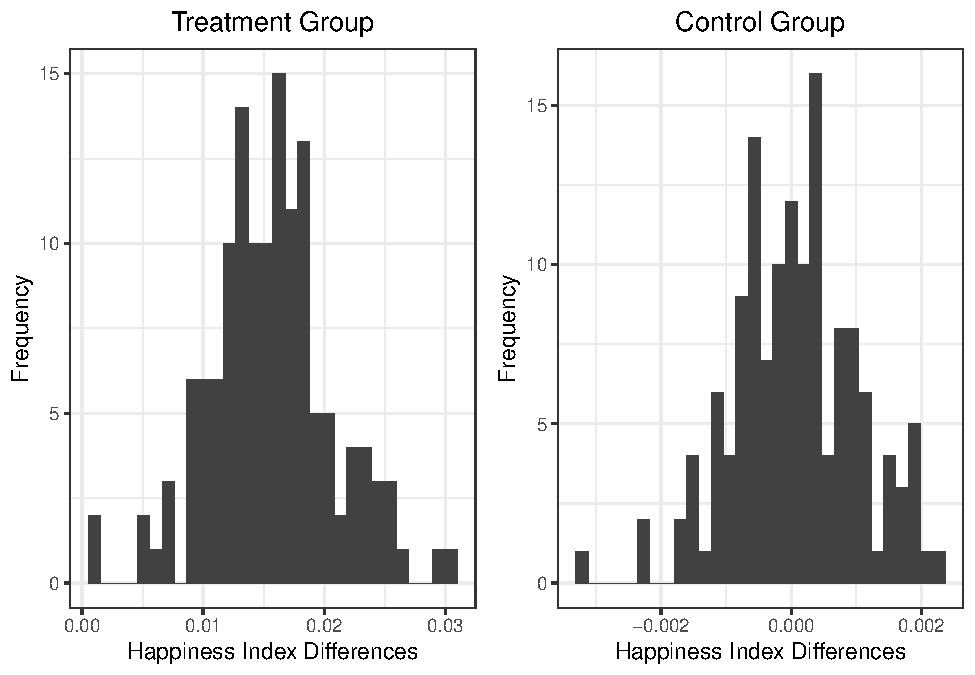
\includegraphics{People_Analytics_Lifecycle_files/figure-latex/pre-post-diff-1} 

}

\caption{Pre/Post Differences for Treatment and Control Groups}\label{fig:pre-post-diff}
\end{figure}

Based on a visual inspection, the distributions of differences appear to be roughly normal. This should not be surprising given random values were sampled from normal distributions to derive artificial post-intervention happiness indices.

Let's test for normality by performing the Shapiro-Wilk test on vectors of differences:

\begin{Shaded}
\begin{Highlighting}[]
\CommentTok{\# Compute Shapiro{-}Wilk test of normality}
\FunctionTok{shapiro.test}\NormalTok{(treat\_metrics}\SpecialCharTok{$}\NormalTok{diff)}
\end{Highlighting}
\end{Shaded}

\begin{verbatim}
## 
##  Shapiro-Wilk normality test
## 
## data:  treat_metrics$diff
## W = 0.98936, p-value = 0.3738
\end{verbatim}

\begin{Shaded}
\begin{Highlighting}[]
\FunctionTok{shapiro.test}\NormalTok{(ctrl\_metrics}\SpecialCharTok{$}\NormalTok{diff)}
\end{Highlighting}
\end{Shaded}

\begin{verbatim}
## 
##  Shapiro-Wilk normality test
## 
## data:  ctrl_metrics$diff
## W = 0.99096, p-value = 0.5134
\end{verbatim}

Since \(p\) \textgreater{} .05 for both tests, the assumption of normally distributed differences is met. Given the data generative process implemented for this example, differences would become increasingly normal as the sample size increases. We now have the greenlight to perform the paired samples \(t\)-test.

We can run a paired samples \(t\)-test in R by passing \texttt{paired\ =\ TRUE} as an argument to the same \texttt{t.test()} function used for the independent samples \(t\)-test. Since we are investigating whether the average post-intervention happiness index is significantly \emph{greater} than the average pre-intervention happiness index, we also need the \texttt{alternative\ =\ "greater"} argument since the default two-tailed test only evaluates whether the average indices are significantly different (regardless of whether the pre- or post-intervention index is larger).

\begin{Shaded}
\begin{Highlighting}[]
\CommentTok{\# Perform one{-}tailed paired samples t{-}test for treatment group}
\FunctionTok{t.test}\NormalTok{(treat\_metrics}\SpecialCharTok{$}\NormalTok{post\_ind, treat\_metrics}\SpecialCharTok{$}\NormalTok{pre\_ind, }\AttributeTok{paired =} \ConstantTok{TRUE}\NormalTok{, }\AttributeTok{alternative =} \StringTok{"greater"}\NormalTok{)}
\end{Highlighting}
\end{Shaded}

\begin{verbatim}
## 
##  Paired t-test
## 
## data:  treat_metrics$post_ind and treat_metrics$pre_ind
## t = 35.906, df = 137, p-value < 2.2e-16
## alternative hypothesis: true difference in means is greater than 0
## 95 percent confidence interval:
##  0.01490482        Inf
## sample estimates:
## mean of the differences 
##              0.01562551
\end{verbatim}

These results indicate that the post-intervention happiness index is significantly larger than the pre-intervention happiness index. This is encouraging with respect to the potential efficacy of the flexible work pilot, but the question about whether the control group experienced a commensurate improvement over the observation period remains unanswered.

Let's run the same paired samples \(t\)-test using the control group indices:

\begin{Shaded}
\begin{Highlighting}[]
\CommentTok{\# Perform one{-}tailed paired samples t{-}test for control group}
\FunctionTok{t.test}\NormalTok{(ctrl\_metrics}\SpecialCharTok{$}\NormalTok{post\_ind, ctrl\_metrics}\SpecialCharTok{$}\NormalTok{pre\_ind, }\AttributeTok{paired =} \ConstantTok{TRUE}\NormalTok{, }\AttributeTok{alternative =} \StringTok{"greater"}\NormalTok{)}
\end{Highlighting}
\end{Shaded}

\begin{verbatim}
## 
##  Paired t-test
## 
## data:  ctrl_metrics$post_ind and ctrl_metrics$pre_ind
## t = 0.59995, df = 138, p-value = 0.2748
## alternative hypothesis: true difference in means is greater than 0
## 95 percent confidence interval:
##  -8.719262e-05           Inf
## sample estimates:
## mean of the differences 
##            4.953658e-05
\end{verbatim}

Since \(p\) \textgreater{} .05, we can conclude that there was not a significant increase in happiness indices for the control group, which provides additional -- but not conclusive -- support for the effectiveness of the flexible work benefit. Chapter \ref{lm} will introduce linear regression, which is a powerful modeling tool for people analytics that helps control for multiple alternative explanations of associations with the DV in order to isolate the unique effects of each IV.

We can evaluate the magnitude of mean differences for these paired samples by passing the \texttt{paired\ =\ TRUE} argument to the same \texttt{cohen.d()} function used for independent samples:

\begin{Shaded}
\begin{Highlighting}[]
\CommentTok{\# Perform Cohen\textquotesingle{}s d}
\NormalTok{effsize}\SpecialCharTok{::}\FunctionTok{cohen.d}\NormalTok{(treat\_metrics}\SpecialCharTok{$}\NormalTok{post\_ind, treat\_metrics}\SpecialCharTok{$}\NormalTok{pre\_ind, }\AttributeTok{paired =} \ConstantTok{TRUE}\NormalTok{)}
\end{Highlighting}
\end{Shaded}

\begin{verbatim}
## 
## Cohen's d
## 
## d estimate: 0.03132117 (negligible)
## 95 percent confidence interval:
##      lower      upper 
## 0.02960345 0.03303890
\end{verbatim}

Though pre/post indices are statistically significant for the treatment group, the size of the difference is negligible (\(d\) = .03).

\textbf{Wilcoxon Signed-Rank Test}

The \textbf{Wilcoxon Signed-Rank Test} is the nonparametric alternative to the paired samples \(t\)-test. This distribution-free test does not require normally distributed differences.

The matched Wilcoxon Signed-Rank test is performed in R using the same \texttt{wilcox.test()} function used to perform the unmatched Wilcoxon Rank-Sum test. Though we can use a paired samples \(t\)-test to test differences for our flexible work benefit study since the assumption of normally distributed differences is met, let's run a Wilcoxon Signed-Rank test for demonstrative purposes:

\begin{Shaded}
\begin{Highlighting}[]
\CommentTok{\# Perform Wilcoxon Signed{-}Rank test}
\FunctionTok{wilcox.test}\NormalTok{(treat\_metrics}\SpecialCharTok{$}\NormalTok{post\_ind, treat\_metrics}\SpecialCharTok{$}\NormalTok{pre\_ind, }\AttributeTok{paired =} \ConstantTok{TRUE}\NormalTok{)}
\end{Highlighting}
\end{Shaded}

\begin{verbatim}
## 
##  Wilcoxon signed rank test with continuity correction
## 
## data:  treat_metrics$post_ind and treat_metrics$pre_ind
## V = 9591, p-value < 2.2e-16
## alternative hypothesis: true location shift is not equal to 0
\end{verbatim}

\begin{Shaded}
\begin{Highlighting}[]
\CommentTok{\# Perform Wilcoxon Signed{-}Rank test}
\FunctionTok{wilcox.test}\NormalTok{(ctrl\_metrics}\SpecialCharTok{$}\NormalTok{post\_ind, ctrl\_metrics}\SpecialCharTok{$}\NormalTok{pre\_ind, }\AttributeTok{paired =} \ConstantTok{TRUE}\NormalTok{)}
\end{Highlighting}
\end{Shaded}

\begin{verbatim}
## 
##  Wilcoxon signed rank test with continuity correction
## 
## data:  ctrl_metrics$post_ind and ctrl_metrics$pre_ind
## V = 5166, p-value = 0.5275
## alternative hypothesis: true location shift is not equal to 0
\end{verbatim}

Consistent with results from the paired samples \(t\)-tests, significantly higher post-intervention happiness indices were observed for the treatment group but not for the control group.

We can evaluate the magnitude of differences for these paired samples by passing the \texttt{paired\ =\ TRUE} argument to the same \texttt{cliff.delta()} function used for independent samples:

\begin{Shaded}
\begin{Highlighting}[]
\CommentTok{\# Run Cliff\textquotesingle{}s Delta}
\NormalTok{effsize}\SpecialCharTok{::}\FunctionTok{cliff.delta}\NormalTok{(treat\_metrics}\SpecialCharTok{$}\NormalTok{post\_ind, treat\_metrics}\SpecialCharTok{$}\NormalTok{pre\_ind, }\AttributeTok{paired =} \ConstantTok{TRUE}\NormalTok{)}
\end{Highlighting}
\end{Shaded}

\begin{verbatim}
## 
## Cliff's Delta
## 
## delta estimate: 0.1544844 (small)
## 95 percent confidence interval:
##      lower      upper 
## 0.01652557 0.28667094
\end{verbatim}

With Cliff's delta, we observe a small difference between pre/post indices for the treatment group (delta estimate = .15).

\textbf{Analysis of Variance (ANOVA)}

\textbf{Analysis of Variance (ANOVA)} is used to determine whether the means of scale-level DVs are equal across nominal-level variables with three or more independent categories.

It is important to understand that \(H_0\) in ANOVA not only requires all group means to be equal but their complex contrasts as well. For example, if we have four groups named A, B, C, and D, \(H_0\) requires that \(\mu_A = \mu_B = \mu_C = \mu_D\) is true as well as the various complex contrasts such as \(\mu_{A,B} = \mu_{C,D}\) and \(\mu_A = \mu_{B,C,D}\) and \(\mu_D = \mu_{B,C}\). Therefore, a difference between one or more of these contrasts results in a decision to reject \(H_0\) in ANOVA. As a result, we may find a significant \(F\)-statistic but no significant differences between pairwise means.

In addition, it is possible to find a significant pairwise mean difference but a non-significant result from ANOVA. As you may recall from Chapter \ref{inf-stats}, multiple comparisons reduce the power of statistical tests. Since multiple tests of mean differences are performed with ANOVA, the family-wise error rate is used to adjust for the increased probability of a Type I error across the set of analyses. Since the power of a single pairwise test is greater relative to the power of familywise comparisons, we may find a significant result for the former but not the latter.

ANOVA requires IVs to be categorical (nominal or ordinal) and the DV to be continuous (interval or ratio). A \textbf{one-way ANOVA} is used to determine how one categorical IV influences a continuous DV. A \textbf{two-way ANOVA} is used to determine how two categorical IVs influence a continuous DV. A \textbf{three-way ANOVA} is used to evaluate how three categorical IVs influence a continuous DV. An ANOVA that uses two or more categorical IVs is often referred to as a \textbf{factorial ANOVA}. As discussed in Chapter \ref{getting-started}, it is important to remain grounded in specific hypotheses, as a significant ANOVA may not actually test what is being hypothesized.

ANOVA is not a test, per se, but a \(F\)-test underpins it. The mathematical procedure behind the \(F\)-test is relatively straightforward:

\begin{enumerate}
\def\labelenumi{\arabic{enumi}.}
\tightlist
\item
  Compute the \textbf{within-group variance}, which is also known as residual variance. Simply put, this tells us how different each member of the group is from the average.
\item
  Compute the \textbf{between-group variance}. This represents how different the group means are from one another.
\item
  Produce the \(F\)-statistic, which is the ratio of \emph{within-group variance} to \emph{between-group variance}.
\end{enumerate}

More formally, the \(F\)-statistic is defined by:

\[ F = \frac{MS_{between}}{MS_{within}}, \]

where:

\[ MS_{between} = \frac{SS_{between}}{df_{between}}, \]

\[ MS_{within} = \frac{SS_{within}}{df_{within}}, \]

\[ SS_{between} = \displaystyle\sum_{j=1}^{p} n_j(\bar{x}_j-\bar{x})^2, \]

\[ SS_{within} = \displaystyle\sum_{j=1}^{p} \displaystyle\sum_{i=1}^{n_j} (x_{ij}-\bar{x_j})^2 \]

\textbf{One-Way ANOVA}

To illustrate how to perform a one-way ANOVA, we will test the hypothesis that mean annual compensation is equal across job satisfaction levels.

Each observation in \texttt{employees} represents a unique employee, and a given employee can only have one job satisfaction score and one annual compensation value. The assumption of independence is met since each record exists independent of one another and each job satisfaction group is comprised of different employees.

Levene's test (Levene, 1960) can be used to test the homogeneity of variance assumption -- even with non-normal distributions. This can be performed in R using the \texttt{leveneTest()} function from the \texttt{car} package:

\begin{Shaded}
\begin{Highlighting}[]
\CommentTok{\# Perform Levene\textquotesingle{}s test for homogeneity of variance}
\NormalTok{car}\SpecialCharTok{::}\FunctionTok{leveneTest}\NormalTok{(annual\_comp }\SpecialCharTok{\textasciitilde{}} \FunctionTok{as.factor}\NormalTok{(job\_sat), }\AttributeTok{data =}\NormalTok{ employees)}
\end{Highlighting}
\end{Shaded}

\begin{verbatim}
## Levene's Test for Homogeneity of Variance (center = median)
##         Df F value Pr(>F)
## group    3  0.3293 0.8042
##       1466
\end{verbatim}

The test statistic associated with Levene's test relates to the null hypothesis that there are no significant differences in variances across the job satisfaction levels. Since \(p > .05\), we fail to reject this null hypothesis and can assume equal variances.

Next, let's test the assumption of normality. It is important to note that the assumption of normality \emph{does not} apply to the distribution of the DV but to the distribution of residuals for each group of the IV. Residuals in the context of ANOVA represent the difference between the actual values of the continuous DV relative to its mean value for each level of the categorical IV (e.g., \(y - \bar{y}_A\), \(y - \bar{y}_B\), \(y - \bar{y}_C\)). In ANOVA, we expect the residuals to be normally distributed around a mean of 0 (the balance point) when the data are normally distributed within each IV category; the more skewed the data, the larger the average distance of each DV value from the mean.

\begin{Shaded}
\begin{Highlighting}[]
\CommentTok{\# Load data viz library}
\FunctionTok{library}\NormalTok{(ggplot2)}
\FunctionTok{library}\NormalTok{(ggpubr)}

\CommentTok{\# Create function to visualize distribution}
\NormalTok{dist.viz }\OtherTok{\textless{}{-}} \ControlFlowTok{function}\NormalTok{(data, x) \{}
  
\NormalTok{viz }\OtherTok{\textless{}{-}}\NormalTok{ ggplot2}\SpecialCharTok{::}\FunctionTok{ggplot}\NormalTok{() }\SpecialCharTok{+} 
\NormalTok{       ggplot2}\SpecialCharTok{::}\FunctionTok{aes}\NormalTok{(data) }\SpecialCharTok{+} 
\NormalTok{       ggplot2}\SpecialCharTok{::}\FunctionTok{labs}\NormalTok{(}\AttributeTok{title =} \FunctionTok{paste}\NormalTok{(}\StringTok{"Job Sat = "}\NormalTok{, x), }\AttributeTok{x =} \StringTok{"Annual Compensation"}\NormalTok{, }\AttributeTok{y =} \StringTok{"Frequency"}\NormalTok{) }\SpecialCharTok{+} 
\NormalTok{       ggplot2}\SpecialCharTok{::}\FunctionTok{geom\_histogram}\NormalTok{(}\AttributeTok{fill =} \StringTok{"\#414141"}\NormalTok{) }\SpecialCharTok{+}
\NormalTok{       ggplot2}\SpecialCharTok{::}\FunctionTok{theme\_bw}\NormalTok{() }\SpecialCharTok{+}
\NormalTok{       ggplot2}\SpecialCharTok{::}\FunctionTok{theme}\NormalTok{(}\AttributeTok{plot.title =} \FunctionTok{element\_text}\NormalTok{(}\AttributeTok{hjust =} \FloatTok{0.5}\NormalTok{))}

  \FunctionTok{return}\NormalTok{(viz)}
\NormalTok{\}}

\CommentTok{\# Produce annual compensation vectors for each job satisfaction level}
\CommentTok{\# Unlist() is needed to convert the default object from subset() into a numeric vector}
\NormalTok{group\_1 }\OtherTok{\textless{}{-}} \FunctionTok{unlist}\NormalTok{(}\FunctionTok{subset}\NormalTok{(employees, job\_sat }\SpecialCharTok{==} \DecValTok{1}\NormalTok{, }\AttributeTok{select =}\NormalTok{ annual\_comp))}
\NormalTok{group\_2 }\OtherTok{\textless{}{-}} \FunctionTok{unlist}\NormalTok{(}\FunctionTok{subset}\NormalTok{(employees, job\_sat }\SpecialCharTok{==} \DecValTok{2}\NormalTok{, }\AttributeTok{select =}\NormalTok{ annual\_comp))}
\NormalTok{group\_3 }\OtherTok{\textless{}{-}} \FunctionTok{unlist}\NormalTok{(}\FunctionTok{subset}\NormalTok{(employees, job\_sat }\SpecialCharTok{==} \DecValTok{3}\NormalTok{, }\AttributeTok{select =}\NormalTok{ annual\_comp))}
\NormalTok{group\_4 }\OtherTok{\textless{}{-}} \FunctionTok{unlist}\NormalTok{(}\FunctionTok{subset}\NormalTok{(employees, job\_sat }\SpecialCharTok{==} \DecValTok{4}\NormalTok{, }\AttributeTok{select =}\NormalTok{ annual\_comp))}

\CommentTok{\# Call UDF to build annual comp histogram for each job satisfaction level}
\NormalTok{viz\_1 }\OtherTok{\textless{}{-}} \FunctionTok{dist.viz}\NormalTok{(}\AttributeTok{data =}\NormalTok{ group\_1, }\AttributeTok{x =} \DecValTok{1}\NormalTok{)}
\NormalTok{viz\_2 }\OtherTok{\textless{}{-}} \FunctionTok{dist.viz}\NormalTok{(}\AttributeTok{data =}\NormalTok{ group\_2, }\AttributeTok{x =} \DecValTok{2}\NormalTok{)}
\NormalTok{viz\_3 }\OtherTok{\textless{}{-}} \FunctionTok{dist.viz}\NormalTok{(}\AttributeTok{data =}\NormalTok{ group\_3, }\AttributeTok{x =} \DecValTok{3}\NormalTok{)}
\NormalTok{viz\_4 }\OtherTok{\textless{}{-}} \FunctionTok{dist.viz}\NormalTok{(}\AttributeTok{data =}\NormalTok{ group\_4, }\AttributeTok{x =} \DecValTok{4}\NormalTok{)}

\CommentTok{\# Display distribution visualizations}
\NormalTok{ggpubr}\SpecialCharTok{::}\FunctionTok{ggarrange}\NormalTok{(viz\_1, viz\_2, viz\_3, viz\_4,}
          \AttributeTok{ncol =} \DecValTok{2}\NormalTok{, }\AttributeTok{nrow =} \DecValTok{2}\NormalTok{)}
\end{Highlighting}
\end{Shaded}

\begin{figure}

{\centering 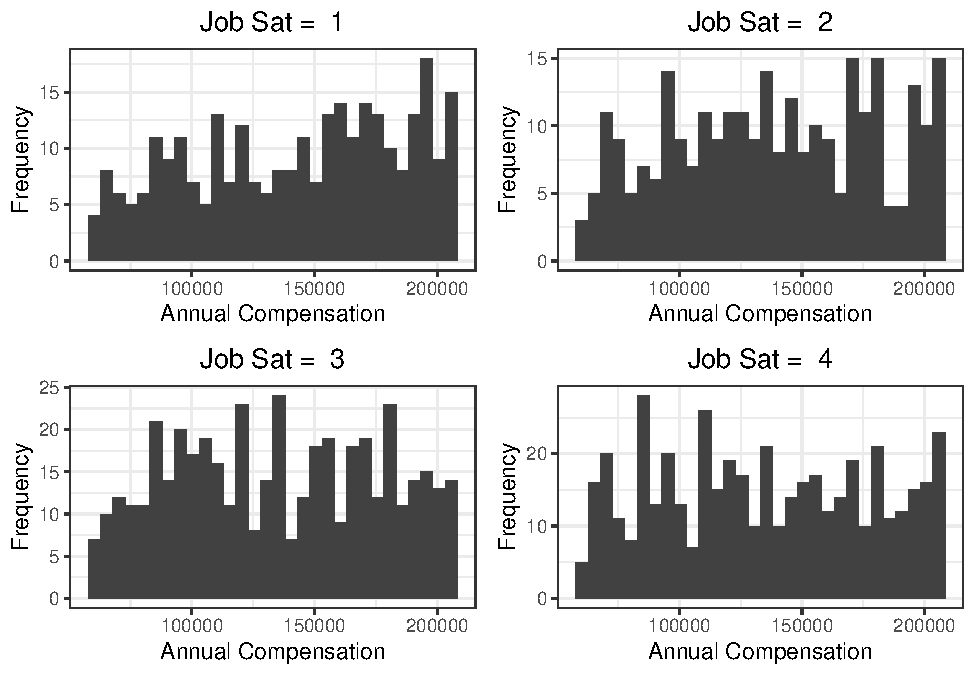
\includegraphics{People_Analytics_Lifecycle_files/figure-latex/comp-dist-1} 

}

\caption{Annual Compensation Distribution by Job Satisfaction Level}\label{fig:comp-dist}
\end{figure}

As we can see, annual compensation data are not normally distributed within job satisfaction groups. Therefore, we would not expect the distribution of residuals to be normally distributed within these groups either.

To test whether the assumption of normality is met, we will first produce and review a \textbf{quantile-quantile (Q-Q) plot}. A Q-Q plot compares two probability distributions by plotting their quantiles (data partitioned into equal-sized groups) against each other. After partitioning annual compensation into groups differentiated by job satisfaction level, we can use the \texttt{ggqqplot()} function from the \texttt{ggpubr} library to build a Q-Q plot and evaluate the distribution of residuals.

\begin{Shaded}
\begin{Highlighting}[]
\CommentTok{\# Generate residuals for each group}
\NormalTok{residuals }\OtherTok{\textless{}{-}} \FunctionTok{c}\NormalTok{(group\_1 }\SpecialCharTok{{-}} \FunctionTok{mean}\NormalTok{(group\_1), group\_2 }\SpecialCharTok{{-}} \FunctionTok{mean}\NormalTok{(group\_2), group\_3 }\SpecialCharTok{{-}} \FunctionTok{mean}\NormalTok{(group\_3), group\_4 }\SpecialCharTok{{-}} \FunctionTok{mean}\NormalTok{(group\_4))}

\CommentTok{\# Create a Q{-}Q plot of residuals}
\NormalTok{ggpubr}\SpecialCharTok{::}\FunctionTok{ggqqplot}\NormalTok{(residuals)}
\end{Highlighting}
\end{Shaded}

\begin{figure}

{\centering 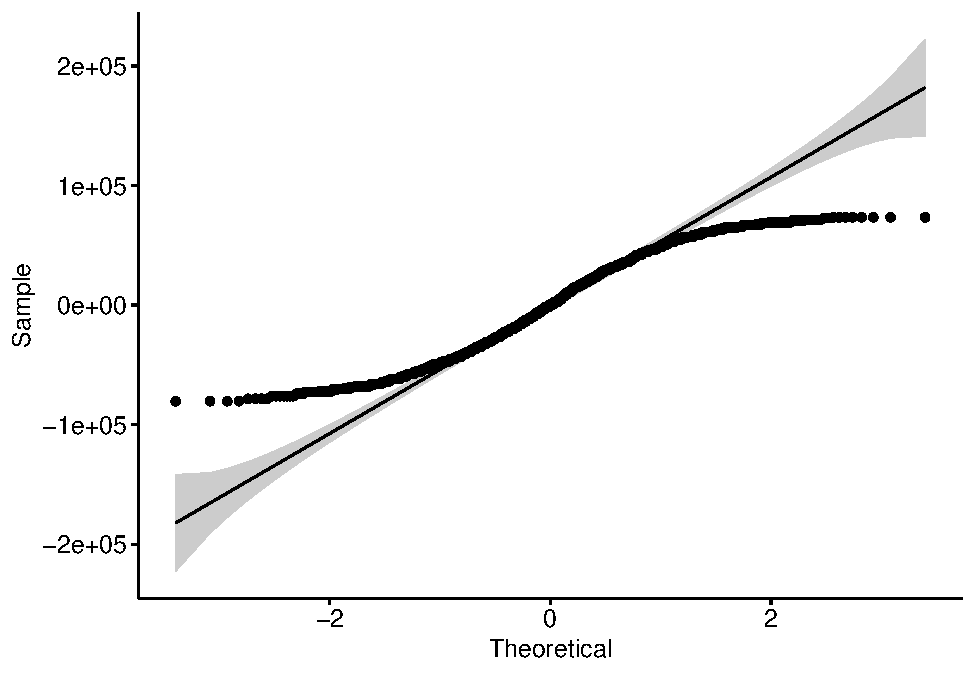
\includegraphics{People_Analytics_Lifecycle_files/figure-latex/qq-plot-1} 

}

\caption{Q-Q Plot of Annual Compensation Residuals}\label{fig:qq-plot}
\end{figure}

To satisfy the assumption of normality, residuals must lie along the linear line. Based on the Q-Q plot in Figure \ref{fig:qq-plot}, there is a clear departure from normality at both ends of the theoretical range.

Let's test for normality using the Shapiro-Wilk test:

\begin{Shaded}
\begin{Highlighting}[]
\CommentTok{\# Compute Shapiro{-}Wilk test of normality}
\FunctionTok{shapiro.test}\NormalTok{(residuals)}
\end{Highlighting}
\end{Shaded}

\begin{verbatim}
## 
##  Shapiro-Wilk normality test
## 
## data:  residuals
## W = 0.95874, p-value < 2.2e-16
\end{verbatim}

Since \(p < .05\), we reject the null hypothesis of normally distributed data, which indicates that the assumption of normality is violated. This should not be surprising based on the deviation from normality we observed in Figure \ref{fig:qq-plot}.

Because the assumption of normality is violated, we have two options. First, we can attempt to transform the data so that the residuals using the transformed values are normally distributed. If the data are resistant to transformation, we can leverage a nonparametric alternative to ANOVA.

Let's first try several common data transformations and then examine the resulting Q-Q plots:

\begin{Shaded}
\begin{Highlighting}[]
\CommentTok{\# Build a linear model using the natural logarithm of annual comp}
\NormalTok{ln.model }\OtherTok{\textless{}{-}} \FunctionTok{lm}\NormalTok{(}\FunctionTok{log}\NormalTok{(annual\_comp) }\SpecialCharTok{\textasciitilde{}}\NormalTok{ job\_sat, }\AttributeTok{data =}\NormalTok{ employees)}

\CommentTok{\# Build a linear model using the log base 10 of annual comp}
\NormalTok{log10.model }\OtherTok{\textless{}{-}} \FunctionTok{lm}\NormalTok{(}\FunctionTok{log10}\NormalTok{(annual\_comp) }\SpecialCharTok{\textasciitilde{}}\NormalTok{ job\_sat, }\AttributeTok{data =}\NormalTok{ employees)}

\CommentTok{\# Build a linear model using the square root of annual comp}
\NormalTok{sqrt.model }\OtherTok{\textless{}{-}} \FunctionTok{lm}\NormalTok{(}\FunctionTok{sqrt}\NormalTok{(annual\_comp) }\SpecialCharTok{\textasciitilde{}}\NormalTok{ job\_sat, }\AttributeTok{data =}\NormalTok{ employees)}

\CommentTok{\# Store Q{-}Q plots to viz objects}
\NormalTok{ln.viz }\OtherTok{\textless{}{-}}\NormalTok{ ggpubr}\SpecialCharTok{::}\FunctionTok{ggqqplot}\NormalTok{(}\FunctionTok{residuals}\NormalTok{(ln.model)) }\SpecialCharTok{+} \FunctionTok{ggtitle}\NormalTok{(}\StringTok{"Natural Log"}\NormalTok{)}
\NormalTok{log10.viz }\OtherTok{\textless{}{-}}\NormalTok{ ggpubr}\SpecialCharTok{::}\FunctionTok{ggqqplot}\NormalTok{(}\FunctionTok{residuals}\NormalTok{(log10.model)) }\SpecialCharTok{+} \FunctionTok{ggtitle}\NormalTok{(}\StringTok{"Log Base 10"}\NormalTok{)}
\NormalTok{sqrt.viz }\OtherTok{\textless{}{-}}\NormalTok{ ggpubr}\SpecialCharTok{::}\FunctionTok{ggqqplot}\NormalTok{(}\FunctionTok{residuals}\NormalTok{(sqrt.model)) }\SpecialCharTok{+} \FunctionTok{ggtitle}\NormalTok{(}\StringTok{"Square Root"}\NormalTok{)}

\CommentTok{\# Display Q{-}Q plots of residuals}
\NormalTok{ggpubr}\SpecialCharTok{::}\FunctionTok{ggarrange}\NormalTok{(ln.viz, log10.viz, sqrt.viz,}
          \AttributeTok{ncol =} \DecValTok{3}\NormalTok{, }\AttributeTok{nrow =} \DecValTok{1}\NormalTok{)}
\end{Highlighting}
\end{Shaded}

\begin{figure}

{\centering 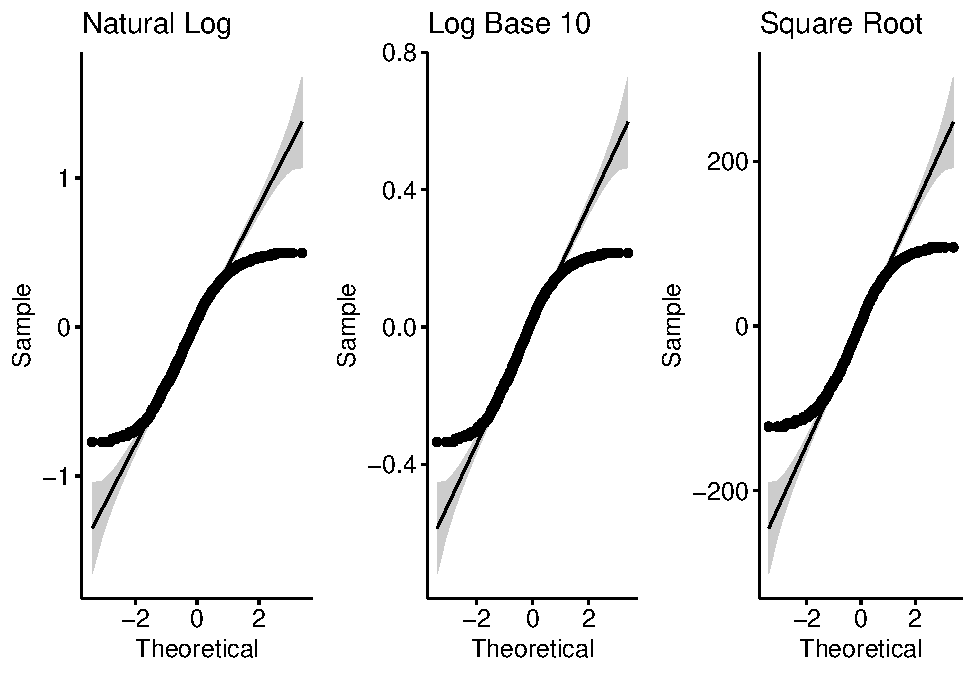
\includegraphics{People_Analytics_Lifecycle_files/figure-latex/qq-plots-trans-1} 

}

\caption{Q-Q Plots of Transformed Annual Compensation Residuals}\label{fig:qq-plots-trans}
\end{figure}

Even with these transformations, there is still a clear S-shaped curve about the residuals. Though we cannot proceed with ANOVA due to violated assumptions, the implementation of ANOVA is demonstrated below. Performing ANOVA involves the \texttt{aov()} function along with the \texttt{summary()} function to display model output:

\begin{Shaded}
\begin{Highlighting}[]
\CommentTok{\# One{-}way ANOVA investigating mean differences in annual comp by job satisfaction}
\NormalTok{one.way }\OtherTok{\textless{}{-}} \FunctionTok{aov}\NormalTok{(annual\_comp }\SpecialCharTok{\textasciitilde{}}\NormalTok{ job\_sat, }\AttributeTok{data =}\NormalTok{ employees)}
\FunctionTok{summary}\NormalTok{(one.way)}
\end{Highlighting}
\end{Shaded}

\begin{verbatim}
##               Df    Sum Sq   Mean Sq F value  Pr(>F)   
## job_sat        1 1.337e+10 1.337e+10   7.508 0.00622 **
## Residuals   1468 2.613e+12 1.780e+09                   
## ---
## Signif. codes:  0 '***' 0.001 '**' 0.01 '*' 0.05 '.' 0.1 ' ' 1
\end{verbatim}

The \textbf{Kruskal Wallis H Test} is the nonparametric alternative to a one-way ANOVA (Daniel, 1990) and an appropriate alternative for investigating median differences in annual comp by job satisfaction in our data. This test can be performed using the \texttt{kruskal.test()} function in R:

\begin{Shaded}
\begin{Highlighting}[]
\CommentTok{\# Nonparametric Kruskal one{-}way ANOVA}
\FunctionTok{kruskal.test}\NormalTok{(annual\_comp }\SpecialCharTok{\textasciitilde{}}\NormalTok{ job\_sat, }\AttributeTok{data =}\NormalTok{ employees)}
\end{Highlighting}
\end{Shaded}

\begin{verbatim}
## 
##  Kruskal-Wallis rank sum test
## 
## data:  annual_comp by job_sat
## Kruskal-Wallis chi-squared = 8.3242, df = 3, p-value = 0.03977
\end{verbatim}

Since \(p < .05\), we can conclude that there are significant differences in median compensation across the groups. However, this test does not indicate which groups are different. We can utilize the \texttt{pairwise.wilcox.test()} function to compute pairwise Wilcoxon rank-sum tests to identify where differences exist:

\begin{Shaded}
\begin{Highlighting}[]
\FunctionTok{pairwise.wilcox.test}\NormalTok{(employees}\SpecialCharTok{$}\NormalTok{annual\_comp, employees}\SpecialCharTok{$}\NormalTok{job\_sat, }\AttributeTok{p.adjust.method =} \StringTok{"BH"}\NormalTok{)}
\end{Highlighting}
\end{Shaded}

\begin{verbatim}
## 
##  Pairwise comparisons using Wilcoxon rank sum test with continuity correction 
## 
## data:  employees$annual_comp and employees$job_sat 
## 
##   1     2     3    
## 2 0.298 -     -    
## 3 0.041 0.298 -    
## 4 0.041 0.298 0.879
## 
## P value adjustment method: BH
\end{verbatim}

Based on the results, there are significant pairwise differences in median annual compensation for job satisfaction levels 3 and 4 relative to level 1.

\textbf{Factorial ANOVA}

\textbf{Factorial ANOVA} is any ANOVA which uses two or more categorical IVs, such as a two-way or three-way ANOVA. It is important to understand the hypothesis a factorial design tests. The following output reflects the cross-tabulation of average annual compensation for each combination of two factors -- job satisfaction and stock option level.

\begin{Shaded}
\begin{Highlighting}[]
\CommentTok{\# Calculate mean for each IV pair}
\NormalTok{combos }\OtherTok{\textless{}{-}} \FunctionTok{aggregate}\NormalTok{(annual\_comp }\SpecialCharTok{\textasciitilde{}}\NormalTok{ job\_sat }\SpecialCharTok{+}\NormalTok{ stock\_opt\_lvl, employees, mean)}
\NormalTok{combos}
\end{Highlighting}
\end{Shaded}

\begin{verbatim}
##    job_sat stock_opt_lvl annual_comp
## 1        1             0    141254.0
## 2        2             0    138753.3
## 3        3             0    132159.2
## 4        4             0    132227.0
## 5        1             1    141763.9
## 6        2             1    135494.5
## 7        3             1    135235.7
## 8        4             1    135569.0
## 9        1             2    146240.0
## 10       2             2    146432.0
## 11       3             2    145080.0
## 12       4             2    143019.3
## 13       1             3    154844.4
## 14       2             3    144254.1
## 15       3             3    135672.7
## 16       4             3    127102.9
\end{verbatim}

As we have already discussed, a difference between one or more of these contrasts may result in a decision to reject \(H_0\) in ANOVA. We may also find a significant pairwise difference but a non-significant result from ANOVA since the family-wise error rate adjustment is applied in the context of multiple comparisons which reduces statistical power.

Factorial ANOVA can be performed by adding variables with \texttt{+} within the same \texttt{aov()} function used for one-way ANOVA:

\begin{Shaded}
\begin{Highlighting}[]
\CommentTok{\# Factorial ANOVA investigating mean differences in annual comp by job satisfaction and stock option level}
\NormalTok{factorial }\OtherTok{\textless{}{-}} \FunctionTok{aov}\NormalTok{(annual\_comp }\SpecialCharTok{\textasciitilde{}}\NormalTok{ job\_sat }\SpecialCharTok{+}\NormalTok{ stock\_opt\_lvl, }\AttributeTok{data =}\NormalTok{ employees)}
\FunctionTok{summary}\NormalTok{(factorial)}
\end{Highlighting}
\end{Shaded}

\begin{verbatim}
##                 Df    Sum Sq   Mean Sq F value  Pr(>F)   
## job_sat          1 1.337e+10 1.337e+10   7.523 0.00617 **
## stock_opt_lvl    1 6.840e+09 6.840e+09   3.850 0.04995 * 
## Residuals     1467 2.606e+12 1.777e+09                   
## ---
## Signif. codes:  0 '***' 0.001 '**' 0.01 '*' 0.05 '.' 0.1 ' ' 1
\end{verbatim}

While mean annual compensation is significantly different by both job satisfaction and stock option level factors, this output alone is not too helpful in understanding the nature of the differences. These statistical significance markers indicate that there are meaningful differences that warrant a deeper understanding. Relationships of job satisfaction and stock option level with annual compensation are illustrated more effectively in Figure \ref{fig:two-way-factorial}.

\begin{figure}

{\centering 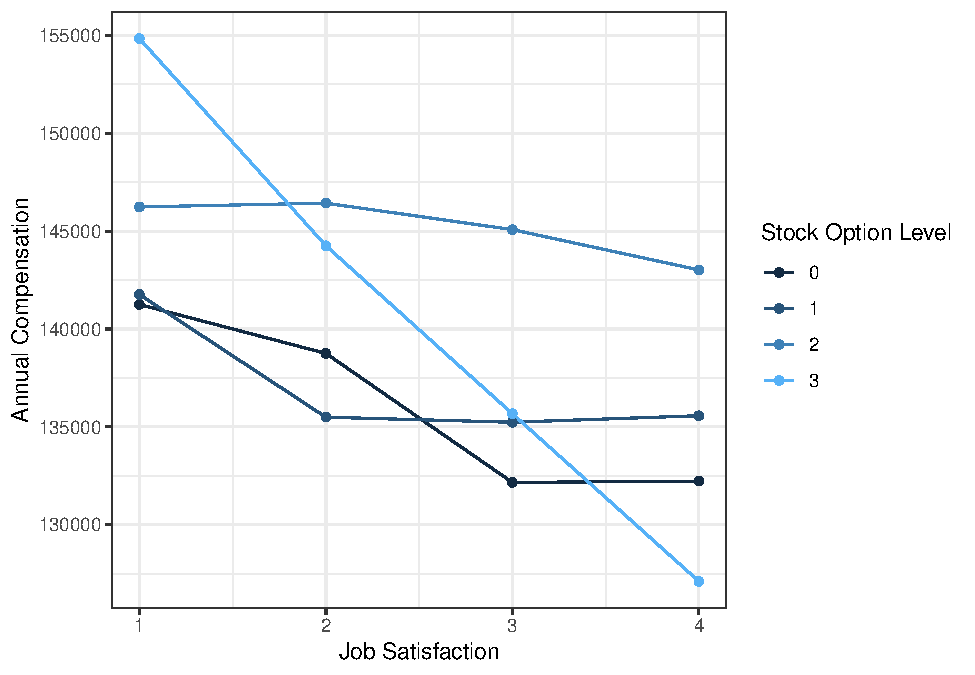
\includegraphics[width=1\linewidth]{People_Analytics_Lifecycle_files/figure-latex/two-way-factorial-1} 

}

\caption{Relationships of Job Satisfaction and Stock Option Level with Annual Compensation}\label{fig:two-way-factorial}
\end{figure}

As we can see, there is a strong negative relationship between job satisfaction and average annual compensation among employees with the highest stock option level (3). The relationship between job satisfaction and average annual compensation appears to be negative for employees with other stock option levels as well, albeit much weaker.

These relationships may initially seem counterintuitive, as one might expect higher levels of job satisfaction to contribute to higher performance and consequently, higher compensation. There may be other variables that happen to be correlated with job satisfaction and/or stock option level that are the actual determinants of annual compensation. For example, there may be a relationship between jobs that each feature a stock option level of 3 but for which there are markedly different average job satisfaction scores and annual compensation among workers in said jobs. Without accounting for additional variables that may explain why employees vary in the amount of annual compensation they earn, the limited set of relationships shown in Figure \ref{fig:two-way-factorial} may lead to a misleading understanding and inaccurate conclusions.

Three-way factorials (and beyond) become difficult to visualize and understand in the way one-way ANOVA and two-way factorials have been explained in this chapter. In Chapter \ref{lm}, we will discuss how to create linear combinations of many IVs and parse the output to understand how they independently and jointly explain variation in the DV.

\hypertarget{review-questions-7}{%
\section{Review Questions}\label{review-questions-7}}

\begin{enumerate}
\def\labelenumi{\arabic{enumi}.}
\item
  What are the main differences between a Chi-square test and Fisher's exact test?
\item
  Why is it problematic to test for significant differences using the \({\chi}^2\) statistic with extremely small samples (e.g., \(n\) \textless{} 5)?
\item
  What are the general assumptions of parametric tests?
\item
  What is a benefit of Welch's \(t\)-test over the Student's \(t\)-test?
\item
  How does a paired-samples \(t\)-test differ from an independent samples \(t\)-test?
\item
  In what ways does the Wilcoxon signed-rank test differ from the paired samples \(t\)-test?
\item
  How can the magnitude of differences (i.e., practical significance) be quantified when working with data measured on a continuous scale?
\item
  How can the magnitude of differences (i.e., practical significance) be quantified when working with data measured on an ordinal scale?
\item
  What null hypothesis does ANOVA test?
\item
  What are some ways to better understand the nature of statistical differences indicated in the output of ANOVA?
\end{enumerate}

\hypertarget{lm}{%
\chapter{Linear Regression}\label{lm}}

It's important to draw a distinction between inferential and predictive models. Inferential models are highly interpretable and their utility is largely in understanding the nature and magnitude of the effect variables have on outcomes. Inferential models also lend to quantifying the extent to which we can generalize the observed effects to the larger population from which the sample was drawn. The objective in predictive modeling is to also to learn from patterns in historical data but for the purpose of achieving the most accurate predictions for future events -- even at the expense of interpretability. To be clear, this isn't to say that predictive models cannot be interpreted -- they certainly can -- but there are relatively few applications for predictive modeling in people analytics because models generally need to be highly interpretable to support action planning.

This chapter is dedicated to inferential modeling to support a working understanding of how to interpret model output and communicate clear, data-driven narratives that respect the nuance and noise characteristic of people data. Chapter \ref{pred-mod} will provide an overview of predictive modeling frameworks.

Regression is perhaps the most important statistical learning technique for people analytics. If you have taken a statistics course at the undergraduate or graduate levels, you have surely already encountered it. Let's first develop an intuitive understanding of the mechanics of regression.

Imagine we are sitting at a large public park in NYC on a nice fall afternoon. If asked to estimate the annual compensation of the next person to walk by, how would you estimate this in the absence of any additional information? Most would likely estimate the \emph{average} annual compensation of everyone capable of walking by. Since this would include both residents and visitors, this would be a very large population of people! The obvious limitation with this approach is that among the large group of people capable of walking by, there is likely a significant range of annual compensation values. Many walking by may be children, unemployed, or retirees who earn no annual compensation, while others may be highly compensated senior executives at the pinnacle of their careers. Since the range of annual compensation could be zero to millions of dollars, estimating the average of such a large population is likely going to be highly inaccurate without more information.

Let's consider that we are sitting outside on a weekday afternoon. Should this influence our annual compensation estimate? It is likely that we can eliminate a large segment of those likely to walk by, as we would expect most children to be in school on a typical fall weekday afternoon. It's also unlikely that those who are employed and not on vacation will walk by on a fall weekday afternoon. Therefore, factoring in that it is a weekday should limit the size of the population which in turn may reduce the range of annual compensation values for our population of passerbys.

Let's now consider that the park is open only to invited guests for a symposium on people analytics. Though it may be difficult to believe, a relatively small subset of the population is likely interested in attending such a symposium, so this information will likely be quite helpful in reducing the size of the population who could walk by. This should further reduce the range of annual compensation since we probably have a good idea of the profile of those most likely to attend. This probably also lessens (or altogether eliminates) the importance of the weekday factor in explaining why people vary in the amount of compensation they earn each year. That an important variable may become unimportant in the presence of another variable is a key feature of regression.

Furthermore, let's consider that only those who reside in NYC and Boise were invited, and that the next person to walk by resides in Boise. Most companies apply a significant cost of living multiplier to the compensation for those in an expensive region such as NYC, resulting in a significant difference in compensation relative to those residing in a much less expensive city like Boise -- all else being equal. Therefore, if we can partition attendees into two groups based on their geography, this should limit the range of annual compensation significantly \emph{within each} -- likely making the average compensation in each group a more nuanced and reasonable estimate.

What if we also learn the specific zip code in which the next passerby from Boise resides? The important information is likely captured at the larger city level (NYC vs.~Boise), as the compensation for the specific zip codes within each city are unlikely to vary to a significant degree. Assuming this is true, it probably would not make sense to consider both the city name and zip code since they are effectively redundant pieces of information with regard to explaining differences in annual compensation.

What if we learn that the next person to walk by will be wearing a blue shirt? Does this influence your estimate? Unless there is research to suggest shirt color and earnings are related, this information will likely not contribute any significant information to our understanding of why people vary in the amount of compensation they earn and should, therefore, not be considered.

You can probably think of many relevant variables that would help further narrow the range of annual compensation. These may include job, level, years of experience, education, among other factors. The main thing to understand is that for each group of observations with the same characteristics -- such as senior analysts with a graduate degree who reside in NYC -- there is a distribution of annual compensation. This distribution reflects unexplained variance. That is, we do not have information to explain why the compensation for each and every person is not the same and in social science contexts, it simply is not practical to explain 100 percent of the variance in outcomes. For example, two people may be similar on dozens of factors (experience, education, skills) but one was simply a more effective negotiator when offered the same role and commanded a higher salary. It's likely we do not have data on salary negotiation ability so this information would leave us with unexplained variance in compensation. The goal is simply to identify the variables that provide the most information in helping us tighten the distribution so that estimating the average value will generally be an accurate estimate for those in the larger population with the same characteristics.

While we can generally improve our estimates with more relevant information (not shirt color or residential zip code in this case), it is important to understand that samples which are too small (\(n\) \textless{} 30) lend to anomalies; modeling noise in sparse data can result in models that are unlikely to generalize beyond the sample data. For example, if the only people from Boise to attend the people analytics symposium happen to be two ultra wealthy tech entrepreneurs who earn millions each year, it would not be appropriate to use this as the basis for our estimates of all future attendees from Boise. This is a phenomenon known as overfitting that will be covered in Chapter \ref{pred-mod}.

This is the essence of linear regression modeling: find a limited number of variables which independently and/or jointly provide significant information that helps explain (by reducing) variance around the average value. As illustrated in this example, adding additional variables (information) can impact the importance of other variables or may offer no incremental information at all. In this chapter, we will cover how to identify which variables are important and how to quantify the effect they have on an outcome.

\textbf{Assumptions \& Diagnostics}

First, the \textbf{sample size} needs to be large enough to model and detect significant associations of one or more predictors with the response variable. In practice, people analytics practitioners are often constrained by the data at hand, which is to say that one generally has little control over the amount of data that can be collected. For example, despite the most earnest participation campaigns, only a subset of invited employees are likely to complete a survey, so collecting additional data to achieve a larger sample is likely not a viable option. It is important to establish a minimum -- and realistic -- \(n\)-count threshold during the planning stage of a project based on the research objectives and variables that need to be factored into the analysis.

Consistent with the assumptions of parametric tests covered in Chapter \ref{aod}, there are several assumptions that need to be validated to determine if a linear model is appropriate for understanding relationships in the data. These assumptions largely relate to the residuals (\(\hat{y}\) - \(y\)):

\begin{enumerate}
\def\labelenumi{\arabic{enumi}.}
\tightlist
\item
  \textbf{Independence}: Residuals are independent of each other; consecutive residuals in time series data are unrelated
\item
  \textbf{Homoscedasticity}: Variance of residuals is constant across values of \(X\)
\item
  \textbf{Normality}: Residuals must be normally distributed (with mean of 0) across values of \(X\)
\item
  \textbf{Linearity}: Relationship between \(X\) and \(Y\) is linear
\end{enumerate}

Beyond these core assumptions for linear models, additional diagnostics are important to incorporate into the early data screening stage:

\begin{enumerate}
\def\labelenumi{\arabic{enumi}.}
\tightlist
\item
  \textbf{High-Leverage Observations}: Influential data that significantly changes the model fit
\item
  \textbf{Collinearity}: Independent variables that are highly correlated (these should be \emph{independent})
\end{enumerate}

\hypertarget{sample-size}{%
\section{Sample Size}\label{sample-size}}

While a general rule-of-thumb for regression analysis is a minimum of a 20:1 ratio of observations to IVs, the power analysis section in Chapter \ref{inf-stats} covered a more rigorous approach to calculating the sample size needed to observe significant effects.

For linear regression, power analysis involves a comparison of model fit between a model with a full set of predictors relative to one with only a subset of the full model's predictors. The function from the \texttt{pwr} library to call is \texttt{pwr.f2.test(u\ =\ ,\ v\ =\ ,\ f2\ =\ ,\ sig.level\ =\ ,\ power\ =\ )}, where \texttt{u} and \texttt{v} are the numerator and denominator degrees of freedom, respectively, and \texttt{f2} is defined as:

\[ f^2 = \frac {R^2_{AB} - R^2_A}{1 - R^2_{AB}}, \]

where \(R^2_{AB}\) represents the variance accounted for by a full model with all predictors, and \(R^2_A\) represents the variance accounted for by a model containing only a subset of the full model's predictors. For example, power analysis can be leveraged in determining the sample size needed for detecting the incremental main effects for a set of predictors beyond the variance accounted for by a set of controls.

\hypertarget{simple-linear-regression}{%
\section{Simple Linear Regression}\label{simple-linear-regression}}

\textbf{Simple linear regression} is a simple technique for estimating the value of a quantitative DV, denoted as \(Y\), on the basis of a single IV, denoted as \(X\). It is assumed that there is an approximately linear relationship between \(X\) and \(Y\). Often, this relationship is expressed as \emph{regressing} \(Y\) on \(X\) and is defined mathematically as:

\[ Y = \beta_0 + \beta_1 X + \epsilon, \]

where \(\beta_0\) is the expected value of \(Y\) when \(X = 0\) (the \emph{intercept}), and \(\beta_1\) represents the average change in \(Y\) for a one-unit increase in \(X\) (the \emph{slope}). \(\beta_0\) and \(\beta_1\) are unknown \emph{parameters} or \emph{coefficients}. The error term, \(\epsilon\), acknowledges that there is variation in \(Y\) not accounted for by this simple linear model. In other words, it is highly unlikely that there is a perfectly linear relationship between \(X\) and \(Y\), as additional variables not included in the model are likely influencing \(Y\).

Once we estimate the unknown model coefficients, \(\beta_0\) and \(\beta_1\), we can estimate \(Y\) for a particular value of \(X\) by calculating:

\[ \hat{y_i} = \hat{\beta}_0 + \hat{\beta_1}x_i, \]

where \(\hat{y}\) represents an estimate of \(Y\) for the \(i\)-ith value of \(X\) equal to \(x\). The \(\hat{}\) symbol is used to denote an estimated value of an unknown coefficient, parameter, or outcome.

The earliest form of linear regression is the \emph{least squares} method, which was developed at the beginning of the nineteenth century and applied to astronomy problems (James, Witten, Hastie, \& Tibshirani, 2013). While there are several approaches to fitting a linear regression model, \textbf{ordinary least squares (OLS)} is the most common. OLS selects coefficients for \(\hat{\beta}_0\) and \(\hat{\beta}_1\) that minimize the residual sum of squares (RSS) defined by:

\[RSS = (y_1 - \hat{\beta}_0 - \hat{\beta}_1x_1)^2 + (y_2 - \hat{\beta}_0 - \hat{\beta}_1x_2)^2 + {...} + (y_n - \hat{\beta}_0 - \hat{\beta}_1x_n)^2\]

For each value of \(X\), OLS fits a model for which the squared difference between the predicted (\(\hat{\beta}_0 + \hat{\beta}_1x_i\)) and actual (\(y_i\)) values are as small as possible. Figure \ref{fig:lm-residuals} illustrates the result of minimizing \(RSS\) using OLS:

\begin{figure}

{\centering \includegraphics[width=1\linewidth]{People_Analytics_Lifecycle_files/figure-latex/lm-residuals-1} 

}

\caption{Minimizing RSS with Ordinary Least Squares (OLS) Fit}\label{fig:lm-residuals}
\end{figure}

The minimizers for the least squares coefficient estimates are defined by:

\[\hat\beta_1 = \frac{\displaystyle\sum_{i=1}^{n}(x_i - \bar{x})(y_i - \bar{y})} {\displaystyle\sum_{i=1}^{n}(x_i - \bar{x})^2}\]

\[\hat\beta_0 = \bar{y} - \hat{\beta}_1 \bar{x},\]

where \(\bar{x}\) and \(\bar{y}\) are sample means.

It is important to understand the role sample size plays in achieving accurate estimates of \(Y\). Figure \ref{fig:lm-fit-compare} illustrates the impact of fitting a model to too few observations. With \(n\) = 2, it would be easy to fit a perfect model to the data; that is, one representing a line that connects the two data points. However, it is highly unlikely that these data points represent the best model for a larger sample, as there would likely be some distribution of \(Y\) for each value of \(X\).

\begin{figure}

{\centering \includegraphics[width=1\linewidth]{People_Analytics_Lifecycle_files/figure-latex/lm-fit-compare-1} 

}

\caption{Left: Least squares regression model fit to n = 2 observations. Right: Least squares regression model fit to n = 20 observations.}\label{fig:lm-fit-compare}
\end{figure}

In R, we can build (or \emph{fit}) a simple linear regression model using the \texttt{lm()} function. The syntax is \texttt{lm(Y\ \textasciitilde{}\ X,\ dataset)}:

\begin{Shaded}
\begin{Highlighting}[]
\CommentTok{\# Load library}
\FunctionTok{library}\NormalTok{(dplyr)}

\CommentTok{\# Load employee data}
\NormalTok{employees }\OtherTok{\textless{}{-}} \FunctionTok{read.csv}\NormalTok{(}\StringTok{"/Users/craig.starbuck/Library/Mobile Documents/com\textasciitilde{}apple\textasciitilde{}CloudDocs/Documents/People Analytics Book/GitHub/peopleanalytics\_lifecycle\_book/data/employees.csv"}\NormalTok{)}

\CommentTok{\# Subset employees data frame; leads are only applicable for those in sales positions}
\NormalTok{data }\OtherTok{\textless{}{-}} \FunctionTok{subset}\NormalTok{(employees, job\_title }\SpecialCharTok{\%in\%} \FunctionTok{c}\NormalTok{(}\StringTok{\textquotesingle{}Sales Executive\textquotesingle{}}\NormalTok{, }\StringTok{\textquotesingle{}Sales Representative\textquotesingle{}}\NormalTok{))}

\CommentTok{\# Regress YTD leads on engagement}
\NormalTok{slm.fit }\OtherTok{\textless{}{-}} \FunctionTok{lm}\NormalTok{(ytd\_leads }\SpecialCharTok{\textasciitilde{}}\NormalTok{ engagement, data)}
\end{Highlighting}
\end{Shaded}

In practice, linear assumptions are rarely -- if ever -- perfectly met, but there must be evidence that the assumptions are \emph{generally} satisfied.

Before performing model diagnostics, it is important to note the following:

\begin{enumerate}
\def\labelenumi{\arabic{enumi}.}
\tightlist
\item
  Collinearity diagnostics are only applicable in the context of multiple regression, as simple linear models have only one IV (this will be covered later in the chapter).
\item
  Outliers are not always an issue, as we discussed in Chapter \ref{data-mgmt-prep}. Figure \ref{fig:high-leverage} illustrates differences between an outlier that does not influence the model fit (left) relative to one which has significant leverage on the model fit (right).
\end{enumerate}

\begin{verbatim}
## 
## Call:
## lm(formula = Y ~ X)
## 
## Residuals:
##     Min      1Q  Median      3Q     Max 
## -1.4332 -0.5482 -0.0275  0.2867  2.6413 
## 
## Coefficients:
##             Estimate Std. Error t value Pr(>|t|)    
## (Intercept)   0.4395     0.4084   1.076    0.296    
## X             3.1303     0.1515  20.659  5.5e-14 ***
## ---
## Signif. codes:  0 '***' 0.001 '**' 0.01 '*' 0.05 '.' 0.1 ' ' 1
## 
## Residual standard error: 0.8829 on 18 degrees of freedom
## Multiple R-squared:  0.9595, Adjusted R-squared:  0.9573 
## F-statistic: 426.8 on 1 and 18 DF,  p-value: 5.498e-14
\end{verbatim}

\begin{verbatim}
## 
## Call:
## lm(formula = Y.out ~ X.out)
## 
## Residuals:
##      Min       1Q   Median       3Q      Max 
## -1.34746 -0.56288 -0.09021  0.29951  2.66197 
## 
## Coefficients:
##             Estimate Std. Error t value Pr(>|t|)    
## (Intercept)   0.5224     0.3399   1.537    0.141    
## X.out         3.0900     0.1077  28.703   <2e-16 ***
## ---
## Signif. codes:  0 '***' 0.001 '**' 0.01 '*' 0.05 '.' 0.1 ' ' 1
## 
## Residual standard error: 0.863 on 19 degrees of freedom
## Multiple R-squared:  0.9775, Adjusted R-squared:  0.9763 
## F-statistic: 823.9 on 1 and 19 DF,  p-value: < 2.2e-16
\end{verbatim}

\begin{verbatim}
## 
## Call:
## lm(formula = Y.lev ~ X.lev)
## 
## Residuals:
##      Min       1Q   Median       3Q      Max 
## -10.3085  -1.8776   0.8556   2.0309   4.8048 
## 
## Coefficients:
##             Estimate Std. Error t value Pr(>|t|)   
## (Intercept)   3.9645     1.3559   2.924  0.00871 **
## X.lev         1.4180     0.4295   3.302  0.00375 **
## ---
## Signif. codes:  0 '***' 0.001 '**' 0.01 '*' 0.05 '.' 0.1 ' ' 1
## 
## Residual standard error: 3.443 on 19 degrees of freedom
## Multiple R-squared:  0.3646, Adjusted R-squared:  0.3311 
## F-statistic:  10.9 on 1 and 19 DF,  p-value: 0.00375
\end{verbatim}

\begin{figure}

{\centering \includegraphics[width=1\linewidth]{People_Analytics_Lifecycle_files/figure-latex/high-leverage-1} 

}

\caption{Left: Model fit with non-influential outlier. Right: Model fit with high leverage outlier. Outlier shown in red. Black solid line represents model fit without outliers. Red dashed line represents model fit with outliers.}\label{fig:high-leverage}
\end{figure}

We can conveniently perform linear model diagnostics using the \texttt{plot()} function in conjunction with the object holding linear model results (\texttt{slm.fit}). This produces the following standard plots shown in Figure \ref{fig:slm-diagnostics}:

\begin{itemize}
\tightlist
\item
  \textbf{Residuals vs Fitted}: Shows how residuals (\(y\)-axis) change across the range of fitted values (\(x\)-axis)
\item
  \textbf{Normal Q-Q}: Compares two probability distributions by plotting their quantiles (data partitioned into equal-sized groups) against each other
\item
  \textbf{Scale-Location}: Shows how \emph{standardized} residuals (\(y\)-axis) change across the range of fitted values (\(x\)-axis)
\item
  \textbf{Residuals vs Leverage}: Shows the leverage of each data point (\(x\)-axis) against their standardized residuals (\(y\)-axis)
\end{itemize}

\begin{figure}

{\centering \includegraphics[width=1\linewidth]{People_Analytics_Lifecycle_files/figure-latex/slm-diagnostics-1} 

}

\caption{Simple linear regression model diagnostics.}\label{fig:slm-diagnostics}
\end{figure}

The \emph{Residuals vs Fitted} and \emph{Scale-Location} plots help evaluate assumptions of homoscedasticity, linearity, and normality -- which are intricately linked. Data are heteroscedastic if there is a flarring or funnel patterning about the residuals across the range of fitted values. That is, there must be a constant variance about the residual errors in order for the assumption of homoscedasticity to be met. This occurs when there is a linear relationship between \(X\) and \(Y\), in which case residuals will be normally distributed around a mean of 0. While the spread of residuals is greater for larger fitted values in this model, resulting in the lower standardized residual error for smaller fitted values indicated in the Scale-Location plot, the slope of the line in the Residuals vs Fitted plot is effectively flat which indicates that the model does not perform significantly better for certain fitted values relative to others.

Cook's distance in the \emph{Residuals vs Leverage} plot provides a measure of how much our model estimates for all observations change if high leverage observations are removed from the data. Higher numbers indicate stronger influence. R conveniently labels the three observations with the highest leverage, though the degree of leverage is only problematic for observations beyond the dashed Cook's distance line. In this case, there are no observations with enough leverage for the dashed Cook's distance line to show on the plot, so no action is warranted.

In addition to the visual inspection, we can perform the \textbf{Breusch-Pagan test} using the \texttt{bptest()} function from the \texttt{lmtest} library to test the null hypothesis that the data are homoscedastic. If \(p\) \textless{} .05 for the test statistic, we reject the null hypothesis and conclude that there is evidence of heteroscedasticity in the data.

\begin{Shaded}
\begin{Highlighting}[]
\CommentTok{\# Run the Breusch{-}Pagan test for evaluate homoscedasticity}
\NormalTok{lmtest}\SpecialCharTok{::}\FunctionTok{bptest}\NormalTok{(slm.fit)}
\end{Highlighting}
\end{Shaded}

\begin{verbatim}
## 
##  studentized Breusch-Pagan test
## 
## data:  slm.fit
## BP = 0.07603, df = 1, p-value = 0.7828
\end{verbatim}

Since \(p\) \textgreater{} .05, we fail to reject the null hypothesis of homoscedasticity; therefore, this assumption is satisified. If this was not the case, a common approach to addressing heteroscedasticity is transforming the response variable by taking the natural logarithm (\texttt{log()}) or square root (\texttt{sqrt()}) of the raw data. While transformations may correct for violations of linear model assumptions, they also result in a less intuitive interpretation of model output relative to the raw untransformed data.

Let's illustrate how to transform the response variable:

\begin{Shaded}
\begin{Highlighting}[]
\CommentTok{\# Square root transformation of YTD leads}
\NormalTok{slm.fit.trans }\OtherTok{\textless{}{-}} \FunctionTok{lm}\NormalTok{(}\FunctionTok{sqrt}\NormalTok{(ytd\_leads) }\SpecialCharTok{\textasciitilde{}}\NormalTok{ engagement, data)}

\CommentTok{\# Natural logarithmic transformation of YTD leads}
\NormalTok{slm.fit.trans }\OtherTok{\textless{}{-}} \FunctionTok{lm}\NormalTok{(}\FunctionTok{log}\NormalTok{(ytd\_leads) }\SpecialCharTok{\textasciitilde{}}\NormalTok{ engagement, data)}
\end{Highlighting}
\end{Shaded}

The \emph{Normal Q-Q Plot} in Figure \ref{fig:slm-diagnostics} is used to test the assumption of normally distributed model residuals. A perfectly normal distribution of residuals will result in data lying along the line situated at 45-degrees from the \(x\)-axis. Based on a visual inspection, our residuals appear to be normally distributed, as there are only a small number of minor departures in the upper and lower ends of the quantile range.

We can also visualize the distribution of model residuals using a histogram. In the majority of cases, the residual should be 0 -- that is, in most cases the model correctly estimates YTD leads resulting in no difference between estimated and observed values (\(\hat{y}\) - \(y\) = 0).

\begin{Shaded}
\begin{Highlighting}[]
\CommentTok{\# Produce histogram to visualize distribution of model residuals}
\NormalTok{ggplot2}\SpecialCharTok{::}\FunctionTok{ggplot}\NormalTok{() }\SpecialCharTok{+} 
\NormalTok{ggplot2}\SpecialCharTok{::}\FunctionTok{aes}\NormalTok{(slm.fit}\SpecialCharTok{$}\NormalTok{residuals) }\SpecialCharTok{+} 
\NormalTok{ggplot2}\SpecialCharTok{::}\FunctionTok{labs}\NormalTok{(}\AttributeTok{x =} \StringTok{"YTD Leads Residuals"}\NormalTok{, }\AttributeTok{y =} \StringTok{"Density"}\NormalTok{) }\SpecialCharTok{+} 
\NormalTok{ggplot2}\SpecialCharTok{::}\FunctionTok{geom\_histogram}\NormalTok{(}\FunctionTok{aes}\NormalTok{(}\AttributeTok{y =}\NormalTok{ ..density..), }\AttributeTok{fill =} \StringTok{"\#414141"}\NormalTok{) }\SpecialCharTok{+}
\NormalTok{ggplot2}\SpecialCharTok{::}\FunctionTok{geom\_density}\NormalTok{(}\AttributeTok{fill =} \StringTok{"\#ADD8E6"}\NormalTok{, }\AttributeTok{alpha =} \FloatTok{0.6}\NormalTok{) }\SpecialCharTok{+}
\NormalTok{ggplot2}\SpecialCharTok{::}\FunctionTok{theme\_bw}\NormalTok{()}
\end{Highlighting}
\end{Shaded}

\begin{figure}

{\centering \includegraphics{People_Analytics_Lifecycle_files/figure-latex/slm-residuals-1} 

}

\caption{Distribution of model residuals.}\label{fig:slm-residuals}
\end{figure}

Based on both the Normal Q-Q Plot and histogram, the residuals conform to the assumption of normality. We can confirm using the Shapiro-Wilk test, in which a non-significant test statistic is sufficient evidence of normality:

\begin{Shaded}
\begin{Highlighting}[]
\CommentTok{\# Compute Shapiro{-}Wilk test of normality}
\FunctionTok{shapiro.test}\NormalTok{(slm.fit}\SpecialCharTok{$}\NormalTok{residuals)}
\end{Highlighting}
\end{Shaded}

\begin{verbatim}
## 
##  Shapiro-Wilk normality test
## 
## data:  slm.fit$residuals
## W = 0.99339, p-value = 0.07029
\end{verbatim}

Let's use the \texttt{flextable} package to present our simple linear model results in an elegant tabular summary:

\begin{Shaded}
\begin{Highlighting}[]
\FunctionTok{library}\NormalTok{(flextable)}

\CommentTok{\# Produce tabular summary for model results using flextable}
\NormalTok{flextable}\SpecialCharTok{::}\FunctionTok{as\_flextable}\NormalTok{(slm.fit)}
\end{Highlighting}
\end{Shaded}

\providecommand{\docline}[3]{\noalign{\global\setlength{\arrayrulewidth}{#1}}\arrayrulecolor[HTML]{#2}\cline{#3}}

\setlength{\tabcolsep}{2pt}

\renewcommand*{\arraystretch}{1.5}

\begin{longtable}[c]{|p{1.13in}|p{0.88in}|p{1.29in}|p{0.75in}|p{0.75in}|p{0.40in}}



\hhline{>{\arrayrulecolor[HTML]{666666}\global\arrayrulewidth=2pt}->{\arrayrulecolor[HTML]{666666}\global\arrayrulewidth=2pt}->{\arrayrulecolor[HTML]{666666}\global\arrayrulewidth=2pt}->{\arrayrulecolor[HTML]{666666}\global\arrayrulewidth=2pt}->{\arrayrulecolor[HTML]{666666}\global\arrayrulewidth=2pt}->{\arrayrulecolor[HTML]{666666}\global\arrayrulewidth=2pt}-}

\multicolumn{1}{!{\color[HTML]{000000}\vrule width 0pt}>{\raggedright}p{\dimexpr 1.13in+0\tabcolsep+0\arrayrulewidth}}{\fontsize{11}{11}\selectfont{\textcolor[HTML]{000000}{\global\setmainfont{Helvetica}{}}}} & \multicolumn{1}{!{\color[HTML]{000000}\vrule width 0pt}>{\raggedleft}p{\dimexpr 0.88in+0\tabcolsep+0\arrayrulewidth}}{\fontsize{11}{11}\selectfont{\textcolor[HTML]{000000}{\global\setmainfont{Helvetica}{Estimate}}}} & \multicolumn{1}{!{\color[HTML]{000000}\vrule width 0pt}>{\raggedleft}p{\dimexpr 1.29in+0\tabcolsep+0\arrayrulewidth}}{\fontsize{11}{11}\selectfont{\textcolor[HTML]{000000}{\global\setmainfont{Helvetica}{Standard\ Error}}}} & \multicolumn{1}{!{\color[HTML]{000000}\vrule width 0pt}>{\raggedleft}p{\dimexpr 0.75in+0\tabcolsep+0\arrayrulewidth}}{\fontsize{11}{11}\selectfont{\textcolor[HTML]{000000}{\global\setmainfont{Helvetica}{t\ value}}}} & \multicolumn{1}{!{\color[HTML]{000000}\vrule width 0pt}>{\raggedleft}p{\dimexpr 0.75in+0\tabcolsep+0\arrayrulewidth}}{\fontsize{11}{11}\selectfont{\textcolor[HTML]{000000}{\global\setmainfont{Helvetica}{Pr(>|t|)}}}} & \multicolumn{1}{!{\color[HTML]{000000}\vrule width 0pt}>{\raggedright}p{\dimexpr 0.4in+0\tabcolsep+0\arrayrulewidth}!{\color[HTML]{000000}\vrule width 0pt}}{\fontsize{11}{11}\selectfont{\textcolor[HTML]{000000}{\global\setmainfont{Helvetica}{}}}} \\

\hhline{>{\arrayrulecolor[HTML]{666666}\global\arrayrulewidth=2pt}->{\arrayrulecolor[HTML]{666666}\global\arrayrulewidth=2pt}->{\arrayrulecolor[HTML]{666666}\global\arrayrulewidth=2pt}->{\arrayrulecolor[HTML]{666666}\global\arrayrulewidth=2pt}->{\arrayrulecolor[HTML]{666666}\global\arrayrulewidth=2pt}->{\arrayrulecolor[HTML]{666666}\global\arrayrulewidth=2pt}-}

\endfirsthead

\hhline{>{\arrayrulecolor[HTML]{666666}\global\arrayrulewidth=2pt}->{\arrayrulecolor[HTML]{666666}\global\arrayrulewidth=2pt}->{\arrayrulecolor[HTML]{666666}\global\arrayrulewidth=2pt}->{\arrayrulecolor[HTML]{666666}\global\arrayrulewidth=2pt}->{\arrayrulecolor[HTML]{666666}\global\arrayrulewidth=2pt}->{\arrayrulecolor[HTML]{666666}\global\arrayrulewidth=2pt}-}

\multicolumn{1}{!{\color[HTML]{000000}\vrule width 0pt}>{\raggedright}p{\dimexpr 1.13in+0\tabcolsep+0\arrayrulewidth}}{\fontsize{11}{11}\selectfont{\textcolor[HTML]{000000}{\global\setmainfont{Helvetica}{}}}} & \multicolumn{1}{!{\color[HTML]{000000}\vrule width 0pt}>{\raggedleft}p{\dimexpr 0.88in+0\tabcolsep+0\arrayrulewidth}}{\fontsize{11}{11}\selectfont{\textcolor[HTML]{000000}{\global\setmainfont{Helvetica}{Estimate}}}} & \multicolumn{1}{!{\color[HTML]{000000}\vrule width 0pt}>{\raggedleft}p{\dimexpr 1.29in+0\tabcolsep+0\arrayrulewidth}}{\fontsize{11}{11}\selectfont{\textcolor[HTML]{000000}{\global\setmainfont{Helvetica}{Standard\ Error}}}} & \multicolumn{1}{!{\color[HTML]{000000}\vrule width 0pt}>{\raggedleft}p{\dimexpr 0.75in+0\tabcolsep+0\arrayrulewidth}}{\fontsize{11}{11}\selectfont{\textcolor[HTML]{000000}{\global\setmainfont{Helvetica}{t\ value}}}} & \multicolumn{1}{!{\color[HTML]{000000}\vrule width 0pt}>{\raggedleft}p{\dimexpr 0.75in+0\tabcolsep+0\arrayrulewidth}}{\fontsize{11}{11}\selectfont{\textcolor[HTML]{000000}{\global\setmainfont{Helvetica}{Pr(>|t|)}}}} & \multicolumn{1}{!{\color[HTML]{000000}\vrule width 0pt}>{\raggedright}p{\dimexpr 0.4in+0\tabcolsep+0\arrayrulewidth}!{\color[HTML]{000000}\vrule width 0pt}}{\fontsize{11}{11}\selectfont{\textcolor[HTML]{000000}{\global\setmainfont{Helvetica}{}}}} \\

\hhline{>{\arrayrulecolor[HTML]{666666}\global\arrayrulewidth=2pt}->{\arrayrulecolor[HTML]{666666}\global\arrayrulewidth=2pt}->{\arrayrulecolor[HTML]{666666}\global\arrayrulewidth=2pt}->{\arrayrulecolor[HTML]{666666}\global\arrayrulewidth=2pt}->{\arrayrulecolor[HTML]{666666}\global\arrayrulewidth=2pt}->{\arrayrulecolor[HTML]{666666}\global\arrayrulewidth=2pt}-}\endhead



\multicolumn{6}{!{\color[HTML]{FFFFFF}\vrule width 0pt}>{\raggedleft}p{\dimexpr 5.21in+10\tabcolsep+5\arrayrulewidth}!{\color[HTML]{FFFFFF}\vrule width 0pt}}{\fontsize{11}{11}\selectfont{\textcolor[HTML]{000000}{\global\setmainfont{Helvetica}{\textit{Signif.\ codes:\ 0\ <=\ '***'\ <\ 0.001\ <\ '**'\ <\ 0.01\ <\ '*'\ <\ 0.05}}}}} \\





\multicolumn{6}{!{\color[HTML]{FFFFFF}\vrule width 0pt}>{\raggedright}p{\dimexpr 5.21in+10\tabcolsep+5\arrayrulewidth}!{\color[HTML]{FFFFFF}\vrule width 0pt}}{\fontsize{11}{11}\selectfont{\textcolor[HTML]{000000}{\global\setmainfont{Helvetica}{}}}} \\





\multicolumn{6}{!{\color[HTML]{FFFFFF}\vrule width 0pt}>{\raggedright}p{\dimexpr 5.21in+10\tabcolsep+5\arrayrulewidth}!{\color[HTML]{FFFFFF}\vrule width 0pt}}{\fontsize{11}{11}\selectfont{\textcolor[HTML]{000000}{\global\setmainfont{Helvetica}{Residual\ standard\ error:\ 5.095\ on\ 407\ degrees\ of\ freedom}}}} \\





\multicolumn{6}{!{\color[HTML]{FFFFFF}\vrule width 0pt}>{\raggedright}p{\dimexpr 5.21in+10\tabcolsep+5\arrayrulewidth}!{\color[HTML]{FFFFFF}\vrule width 0pt}}{\fontsize{11}{11}\selectfont{\textcolor[HTML]{000000}{\global\setmainfont{Helvetica}{Multiple\ R-squared:\ 0.8858,\ Adjusted\ R-squared:\ 0.8855}}}} \\





\multicolumn{6}{!{\color[HTML]{FFFFFF}\vrule width 0pt}>{\raggedright}p{\dimexpr 5.21in+10\tabcolsep+5\arrayrulewidth}!{\color[HTML]{FFFFFF}\vrule width 0pt}}{\fontsize{11}{11}\selectfont{\textcolor[HTML]{000000}{\global\setmainfont{Helvetica}{F-statistic:\ 3158\ on\ 407\ and\ 1\ DF,\ p-value:\ 0.0000}}}} \\

\endfoot



\multicolumn{1}{!{\color[HTML]{000000}\vrule width 0pt}>{\raggedright}p{\dimexpr 1.13in+0\tabcolsep+0\arrayrulewidth}}{\fontsize{11}{11}\selectfont{\textcolor[HTML]{000000}{\global\setmainfont{Helvetica}{(Intercept)}}}} & \multicolumn{1}{!{\color[HTML]{000000}\vrule width 0pt}>{\raggedleft}p{\dimexpr 0.88in+0\tabcolsep+0\arrayrulewidth}}{\fontsize{11}{11}\selectfont{\textcolor[HTML]{000000}{\global\setmainfont{Helvetica}{1.630}}}} & \multicolumn{1}{!{\color[HTML]{000000}\vrule width 0pt}>{\raggedleft}p{\dimexpr 1.29in+0\tabcolsep+0\arrayrulewidth}}{\fontsize{11}{11}\selectfont{\textcolor[HTML]{000000}{\global\setmainfont{Helvetica}{0.997}}}} & \multicolumn{1}{!{\color[HTML]{000000}\vrule width 0pt}>{\raggedleft}p{\dimexpr 0.75in+0\tabcolsep+0\arrayrulewidth}}{\fontsize{11}{11}\selectfont{\textcolor[HTML]{000000}{\global\setmainfont{Helvetica}{1.635}}}} & \multicolumn{1}{!{\color[HTML]{000000}\vrule width 0pt}>{\raggedleft}p{\dimexpr 0.75in+0\tabcolsep+0\arrayrulewidth}}{\fontsize{11}{11}\selectfont{\textcolor[HTML]{000000}{\global\setmainfont{Helvetica}{0.1028}}}} & \multicolumn{1}{!{\color[HTML]{000000}\vrule width 0pt}>{\raggedright}p{\dimexpr 0.4in+0\tabcolsep+0\arrayrulewidth}!{\color[HTML]{000000}\vrule width 0pt}}{\fontsize{11}{11}\selectfont{\textcolor[HTML]{000000}{\global\setmainfont{Helvetica}{\ \ \ }}}} \\





\multicolumn{1}{!{\color[HTML]{000000}\vrule width 0pt}>{\raggedright}p{\dimexpr 1.13in+0\tabcolsep+0\arrayrulewidth}}{\fontsize{11}{11}\selectfont{\textcolor[HTML]{000000}{\global\setmainfont{Helvetica}{engagement}}}} & \multicolumn{1}{!{\color[HTML]{000000}\vrule width 0pt}>{\raggedleft}p{\dimexpr 0.88in+0\tabcolsep+0\arrayrulewidth}}{\fontsize{11}{11}\selectfont{\textcolor[HTML]{000000}{\global\setmainfont{Helvetica}{20.065}}}} & \multicolumn{1}{!{\color[HTML]{000000}\vrule width 0pt}>{\raggedleft}p{\dimexpr 1.29in+0\tabcolsep+0\arrayrulewidth}}{\fontsize{11}{11}\selectfont{\textcolor[HTML]{000000}{\global\setmainfont{Helvetica}{0.357}}}} & \multicolumn{1}{!{\color[HTML]{000000}\vrule width 0pt}>{\raggedleft}p{\dimexpr 0.75in+0\tabcolsep+0\arrayrulewidth}}{\fontsize{11}{11}\selectfont{\textcolor[HTML]{000000}{\global\setmainfont{Helvetica}{56.193}}}} & \multicolumn{1}{!{\color[HTML]{000000}\vrule width 0pt}>{\raggedleft}p{\dimexpr 0.75in+0\tabcolsep+0\arrayrulewidth}}{\fontsize{11}{11}\selectfont{\textcolor[HTML]{000000}{\global\setmainfont{Helvetica}{0.0000}}}} & \multicolumn{1}{!{\color[HTML]{000000}\vrule width 0pt}>{\raggedright}p{\dimexpr 0.4in+0\tabcolsep+0\arrayrulewidth}!{\color[HTML]{000000}\vrule width 0pt}}{\fontsize{11}{11}\selectfont{\textcolor[HTML]{000000}{\global\setmainfont{Helvetica}{***}}}} \\

\hhline{>{\arrayrulecolor[HTML]{666666}\global\arrayrulewidth=2pt}->{\arrayrulecolor[HTML]{666666}\global\arrayrulewidth=2pt}->{\arrayrulecolor[HTML]{666666}\global\arrayrulewidth=2pt}->{\arrayrulecolor[HTML]{666666}\global\arrayrulewidth=2pt}->{\arrayrulecolor[HTML]{666666}\global\arrayrulewidth=2pt}->{\arrayrulecolor[HTML]{666666}\global\arrayrulewidth=2pt}-}



\end{longtable}

There are several important pieces of information in this output:

\begin{itemize}
\tightlist
\item
  \texttt{Estimate}: \emph{Unstandardized} Beta coefficient associated with the predictor
\item
  \texttt{Standard\ Error}: Average distance between the observed and estimated values per the fitted regression line
\item
  \texttt{t\ value}: \texttt{Estimate} / \texttt{Standard\ Error}. Larger values provide more evidence for a non-zero coefficient (relationship) in the population.
\item
  \texttt{Pr(\textgreater{}\textbar{}t\textbar{})}: \(p\)-value for evaluating whether there is sufficient evidence in the sample that the coefficient (relationship) between the respective predictor and response variable is not 0 in the population (i.e., \(x\) has a relationship with \(y\))
\item
  \texttt{Intercept}: Mean value of the response variable when all predictors are equal to 0. Note that the interpretation of the intercept is often nonsensical since many predictors cannot have 0 values (e.g., age, height, weight, IQ).
\item
  \texttt{Signif.\ codes}: Symbols to quickly ascertain whether predictors are significant at key levels, such as \(p\) \textless{} .001, \(p\) \textless{} .01, or \(p\) \textless{} .05.
\item
  \texttt{Residual\ standard\ error}: Measure of model fit which reflects the standard deviation of the residuals (\(\sqrt {\sum(y-\hat{y})^2 / df}\))
\item
  \texttt{Degrees\ of\ freedom}: \(n\) - \(p\), where \(n\) is the number of observations and \(p\) is the number of predictors
\item
  \texttt{Multiple\ R-squared}: Percent of variance in \(y\) (when multiplied by 100) explained by the predictors in the model. This is also known as the \textbf{Coefficient of Determination}. For simple linear regression, this is simply the squared value of Pearson's \(r\) for the bivariate relationship between the predictor and response (execute \texttt{cor(data\$engagement,\ data\$ytd\_leads)\^{}2} to validate).
\item
  \texttt{Adjusted\ R-squared}: Modified version of \(R^2\) that adjusts the estimate for non-significant predictors. A large delta between \(R^2\) and Adjusted \(R^2\) coefficients generally indicates a model containing a larger number of non-significant predictors relative to when \(R^2\) and Adjusted \(R^2\) values are similar.
\item
  \texttt{F-statistic}: Statistic used in conjunction with the \texttt{p-value} for testing differences between the specified model and an intercept-only model (a model with no predictors). This test helps us evaluate whether our predictors are helpful in explaining variance in \(y\).
\end{itemize}

The output of this simple linear regression model indicates that for each level increase in engagement, the average increase in YTD leads is about 20 (\(\beta\) = 20.1, \(t\)(407) = 56.2, \(p\) \textless{} .001). Had we transformed the response variable from its original unit of measurement, the interpretation would be expressed in the transformed units (e.g., \(\beta\) is the square root or natural log of the average change in leads for a one-level increase in engagement).

Thanks to the properties of the CLT, which requires normally distributed \emph{residuals}, we can be confident that the true relationship between engagement and YTD leads in the population is not 0 since the 95\% CI (\(\beta\) +/- 2\(SE\)) does not include 0.

While it may be tempting to conclude that employee engagement has a significant influence on leads based on the model output, we know that bivariate relationships may be spurious; that is, engagement may be correlated with another variable that is actually influencing leads. In practice, a simple linear model is rarely sufficient for explaining a meaningful percent of variance in a response variable, and additional predictors are usually needed to capture the complex and nuanced relationships characteristic of people analytics problems.

The \(R^2\) value indicates that 8.9\% of the variance in leads can be explained by the variation in engagement levels. Put differently, this simple model does not account for 91.1\% of variation in leads. Since a large portion of the variance in leads is unexplained, we need signal from additional predictors to understand the other dimensions along which leads vary.

Figure \ref{fig:slm-fit} illustrates how the regression equation for this simple linear model (\(y\) = 20.1\(x\) + 1.6) fits the data points for sales employees. The spread of leads at each engagement level indicates that there are other factors that explain variance in leads that need to be accounted for in the regression equation to achieve more accurate estimates. The reduction in the spread of leads for a combination of significant predictor values increases \(R^2\) (explained variance in YTD leads).

\begin{figure}

{\centering \includegraphics[width=1\linewidth]{People_Analytics_Lifecycle_files/figure-latex/slm-fit-1} 

}

\caption{Simple Linear Model Fit Line for y = 20.1x + 1.6}\label{fig:slm-fit}
\end{figure}

We can use the \texttt{extract\_eq()} function from the \texttt{equatiomatic} library to easily build a properly formatted LaTex regression equation from the model object:

\begin{Shaded}
\begin{Highlighting}[]
\CommentTok{\# Load library}
\FunctionTok{library}\NormalTok{(equatiomatic)}

\CommentTok{\# Convert model to LaTex regression equation}
\FunctionTok{extract\_eq}\NormalTok{(slm.fit)}
\end{Highlighting}
\end{Shaded}

\begin{equation}
\operatorname{ytd\_leads} = \alpha + \beta_{1}(\operatorname{engagement}) + \epsilon
\end{equation}

\hypertarget{multiple-linear-regression}{%
\section{Multiple Linear Regression}\label{multiple-linear-regression}}

\textbf{Multiple linear regression} extends the simple linear model to one with two or more predictor variables. A multiple regression model generally explains more variance in the response relative to the simple linear model, and is defined by:

\[ Y = \beta_0 + \beta_1 X_1 + \beta_2 X_2 + {...} + \beta_p X_p + \epsilon \]

Once we estimate the unknown model coefficients, \(\beta_0\) through \(\beta_p\), we can estimate \(Y\) for a particular combination of values for \(X_1\) through \(X_p\) by calculating:

\[ \hat{y_i} = \hat{\beta}_0 + \hat{\beta_1}x_{i1} + \hat{\beta_2}x_{i2} + {...} + \hat{\beta_p} x_{ip} \]

\textbf{Collinearity Diagnostics}

In addition to the assumptions we tested in the context of the simple linear model, multiple linear regression warrants collinearity diagnostics. \textbf{Collinearity} refers to situations in which predictors that are related to the response variable also have strong associations with one another. In practice, there is usually some level of collinearity between variables, so the goal of collinearity diagnostics is to identify and address \emph{problematic} levels of collinearity.

Models should be built with predictors that have a strong association with the outcome but not with one another. If predictors are highly correlated with each other, it indicates that they are redundant and do not provide unique information. A large amount of collinearity can cause serious issues with the underlying calculus of a regression model, which can manifest in the form of effects of significant predictors being masked or suppressed or a negative sign/effect showing in the output when a positive association between the predictor and the response actually exists (or vice versa). As a result, it would be premature to fit a linear model before running collinearity diagnostics, as there may be false negatives -- predictors that appear unimportant but are actually statistical drivers of the response. If problematic collinearity is not addressed, false conclusions may be drawn from the model output which may lead to bad business decisions.

Kuhn and Johnson (2013) recommend the simple procedure outlined below to identify and address problematic collinearity:

\begin{enumerate}
\def\labelenumi{\arabic{enumi}.}
\tightlist
\item
  Determine the two predictors associated with the largest absolute pairwise correlation (whether they are positively or negatively related does not matter) -- call them predictors A and B.
\item
  Determine the average absolute correlation between predictor A and the other variables. Do the same for predictor B.
\item
  If predictor A has a larger average absolute correlation, remove it; otherwise, remove predictor B. The exception to this rule is when predictors A and B have similar average absolute correlations with all other predictors but the predictor with the slightly higher correlation is a key variable that, if dropped, will prevent you from addressing one or more stated objectives or hypotheses.
\item
  Repeat steps 1-3 until \(|r|\) \textless{} .7.
\end{enumerate}

Let's demonstrate the procedures and mechanics for multiple linear regression by estimating YTD sales using multiple predictor variables. While not appropriate in practice, we will select a subset of the available predictors from \texttt{data} to simplify the model and explanation. In Chapter \ref{pred-mod}, we will discuss the use of machine learning (ML) models for more efficient and comprehensive variable selection.

We can leverage the \texttt{ggpairs()} function introduced in Chapter \ref{desc-stats} to efficiently compute bivariate correlations and visualize data distributions:

\begin{figure}

{\centering \includegraphics[width=1\linewidth]{People_Analytics_Lifecycle_files/figure-latex/ggpairs-ytd-sales-1} 

}

\caption{GGpairs bivariate correlations and data distributions.}\label{fig:ggpairs-ytd-sales}
\end{figure}

Based on the correlations, \texttt{org\_tenure} is highly correlated with both \texttt{job\_tenure}, \texttt{mgr\_tenure} and \texttt{work\_exp}. These relationships indicate that job and manager changes for those in sales roles have been infrequent since joining the organization, and that a large portion of their work experience has been with this organization. Since \texttt{org\_tenure} has the strongest relationship with our response, \texttt{ytd\_sales}, we will drop \texttt{job\_tenure}, \texttt{mgr\_tenure}, and \texttt{work\_exp}.

Since \(|r|\) \textless{} .7 for all pairwise relationships, let's fit the more parsimonious multiple regression model using the resulting subset of predictors. We can include multiple predictors in the model using the \texttt{+} symbol in the \texttt{lm()} function:

\begin{Shaded}
\begin{Highlighting}[]
\CommentTok{\# Regress YTD sales on a combination of predictors}
\NormalTok{mlm.fit }\OtherTok{\textless{}{-}} \FunctionTok{lm}\NormalTok{(ytd\_sales }\SpecialCharTok{\textasciitilde{}}\NormalTok{ engagement }\SpecialCharTok{+}\NormalTok{ job\_lvl }\SpecialCharTok{+}\NormalTok{ stock\_opt\_lvl }\SpecialCharTok{+}\NormalTok{ org\_tenure, data)}
\end{Highlighting}
\end{Shaded}

While Kuhn and Johnson's procedure is a good first step, this may not eliminate what is known as \textbf{multicollinearity}, which is collinearity among three or more predictors. It is possible for collinearity to exist between three or more variables, even in the absence of a strong correlation for a pair of variables. We can evaluate the \textbf{Variance Inflation Factor (VIF)} for the predictors that remain following the bivariate correlation review to ensure multicollinearity is not present. \(VIF\) is defined by:

\[ VIF(\hat{\beta_j}) = \frac{1}{1 - R^2_{X_j|X_{-j}}}, \]

where the denominator, \(R^2_{X_j|X_{-j}}\), is the \(R^2\) from regressing \(X_j\) onto all other predictors. The smallest value of \(VIF\) is 1, which indicates a complete absence of collinearity. Problematic collinearity exists if \(VIF\) for any variable exceeds 5.

We can produce \(VIF\) for each variable using the \texttt{vif()} function from the \texttt{car} library:

\begin{Shaded}
\begin{Highlighting}[]
\CommentTok{\# Load library}
\FunctionTok{library}\NormalTok{(car)}

\CommentTok{\# Produce VIF for each predictor}
\NormalTok{car}\SpecialCharTok{::}\FunctionTok{vif}\NormalTok{(mlm.fit)}
\end{Highlighting}
\end{Shaded}

\begin{verbatim}
##    engagement       job_lvl stock_opt_lvl    org_tenure 
##      1.001459      1.407192      1.009435      1.395797
\end{verbatim}

Based on the output, \(VIF\) \textless{} 5 for each predictor, which indicates that multicollinearity is not an issue.

Next, let's evaluate the linear model assumptions to validate that fitting a linear model to these data is appropriate:

\begin{figure}

{\centering \includegraphics[width=1\linewidth]{People_Analytics_Lifecycle_files/figure-latex/pre-mlm-diagnostics-1} 

}

\caption{Multiple linear regression model diagnostics.}\label{fig:pre-mlm-diagnostics}
\end{figure}

Based on these visuals, there are obvious violations of linear model assumptions that need to first be addressed.

First, given the long right tail for the \texttt{ytd\_sales} distribution shown in Figure \ref{fig:pre-mlm-diagnostics}, let's apply a square root transformation to the response variable:

\begin{Shaded}
\begin{Highlighting}[]
\CommentTok{\# Regress YTD sales on a combination of predictors}
\NormalTok{mlm.fit }\OtherTok{\textless{}{-}} \FunctionTok{lm}\NormalTok{(}\FunctionTok{sqrt}\NormalTok{(ytd\_sales) }\SpecialCharTok{\textasciitilde{}}\NormalTok{ engagement }\SpecialCharTok{+}\NormalTok{ job\_lvl }\SpecialCharTok{+}\NormalTok{ stock\_opt\_lvl }\SpecialCharTok{+}\NormalTok{ org\_tenure, data)}
\end{Highlighting}
\end{Shaded}

Additionally, the diagnostic plots indicate that there are data points with high leverage on the fit. Let's address using Cook's distance as the criterion:

\begin{Shaded}
\begin{Highlighting}[]
\CommentTok{\# Remove high leverage observations per Cook\textquotesingle{}s distance}
\NormalTok{w }\OtherTok{\textless{}{-}} \FunctionTok{abs}\NormalTok{(}\FunctionTok{rstudent}\NormalTok{(mlm.fit)) }\SpecialCharTok{\textless{}} \DecValTok{3} \SpecialCharTok{\&} \FunctionTok{abs}\NormalTok{(}\FunctionTok{cooks.distance}\NormalTok{(mlm.fit)) }\SpecialCharTok{\textless{}} \DecValTok{4}\SpecialCharTok{/}\FunctionTok{nrow}\NormalTok{(mlm.fit}\SpecialCharTok{$}\NormalTok{model)}
\NormalTok{mlm.fit }\OtherTok{\textless{}{-}} \FunctionTok{update}\NormalTok{(mlm.fit, }\AttributeTok{weights =} \FunctionTok{as.numeric}\NormalTok{(w))}
\end{Highlighting}
\end{Shaded}

Now we can produce a refreshed set of diagnostic plots to evaluate the impact of transforming the response variable and removing high leverage observations:

\begin{figure}

{\centering \includegraphics[width=1\linewidth]{People_Analytics_Lifecycle_files/figure-latex/post-mlm-diagnostics-1} 

}

\caption{Multiple linear regression model diagnostics (post-transformation).}\label{fig:post-mlm-diagnostics}
\end{figure}

There is a clear improvement towards satisifying linear model assumptions.

Let's perform the Breusch-Pagan test to validate that the assumption of homoscedasticity is met:

\begin{Shaded}
\begin{Highlighting}[]
\CommentTok{\# Run the Breusch{-}Pagan test for evaluate homoscedasticity}
\NormalTok{lmtest}\SpecialCharTok{::}\FunctionTok{bptest}\NormalTok{(mlm.fit)}
\end{Highlighting}
\end{Shaded}

\begin{verbatim}
## 
##  studentized Breusch-Pagan test
## 
## data:  mlm.fit
## BP = 2.2111, df = 4, p-value = 0.697
\end{verbatim}

Next, let's ensure residuals are normally distributed around 0:

\begin{Shaded}
\begin{Highlighting}[]
\CommentTok{\# Produce histogram to visualize distribution of model residuals}
\NormalTok{ggplot2}\SpecialCharTok{::}\FunctionTok{ggplot}\NormalTok{() }\SpecialCharTok{+} 
\NormalTok{ggplot2}\SpecialCharTok{::}\FunctionTok{aes}\NormalTok{(mlm.fit}\SpecialCharTok{$}\NormalTok{residuals) }\SpecialCharTok{+} 
\NormalTok{ggplot2}\SpecialCharTok{::}\FunctionTok{labs}\NormalTok{(}\AttributeTok{x =} \StringTok{"YTD Leads Residuals"}\NormalTok{, }\AttributeTok{y =} \StringTok{"Density"}\NormalTok{) }\SpecialCharTok{+} 
\NormalTok{ggplot2}\SpecialCharTok{::}\FunctionTok{geom\_histogram}\NormalTok{(}\FunctionTok{aes}\NormalTok{(}\AttributeTok{y =}\NormalTok{ ..density..), }\AttributeTok{fill =} \StringTok{"\#414141"}\NormalTok{) }\SpecialCharTok{+}
\NormalTok{ggplot2}\SpecialCharTok{::}\FunctionTok{geom\_density}\NormalTok{(}\AttributeTok{fill =} \StringTok{"\#ADD8E6"}\NormalTok{, }\AttributeTok{alpha =} \FloatTok{0.6}\NormalTok{) }\SpecialCharTok{+}
\NormalTok{ggplot2}\SpecialCharTok{::}\FunctionTok{theme\_bw}\NormalTok{()}
\end{Highlighting}
\end{Shaded}

\begin{figure}

{\centering \includegraphics{People_Analytics_Lifecycle_files/figure-latex/mlm-residuals-1} 

}

\caption{Distribution of model residuals}\label{fig:mlm-residuals}
\end{figure}

\begin{Shaded}
\begin{Highlighting}[]
\CommentTok{\# Compute Shapiro{-}Wilk test of normality}
\FunctionTok{shapiro.test}\NormalTok{(mlm.fit}\SpecialCharTok{$}\NormalTok{residuals)}
\end{Highlighting}
\end{Shaded}

\begin{verbatim}
## 
##  Shapiro-Wilk normality test
## 
## data:  mlm.fit$residuals
## W = 0.99342, p-value = 0.07202
\end{verbatim}

Based on the diagnostic plots and statistical tests, our data satisify the requirements for building a multiple linear regression model.

\textbf{Variable Selection}

Next, we need to reduce our model to the subset of predictors with statistically significant relationships with the response variable. \textbf{Backward Stepwise Selection} is a common and simple variable selection procedure, and the steps are outlined below:

\begin{enumerate}
\def\labelenumi{\arabic{enumi}.}
\tightlist
\item
  Remove the predictor with the highest \(p\)-value greater than the critical value (\(\alpha\) = .05).
\item
  Refit the model, and repeat step 1.
\item
  Stop when all \(p\)-values are less than the critical value.
\end{enumerate}

Each predictor in our model has a statistically significant relationship with \texttt{ytd\_sales} -- indicating that the slope of the relationships with the response is unlikely 0 in the population -- so further variable reduction is not required.

\providecommand{\docline}[3]{\noalign{\global\setlength{\arrayrulewidth}{#1}}\arrayrulecolor[HTML]{#2}\cline{#3}}

\setlength{\tabcolsep}{2pt}

\renewcommand*{\arraystretch}{1.5}

\begin{longtable}[c]{|p{1.17in}|p{0.88in}|p{1.29in}|p{0.75in}|p{0.75in}|p{0.40in}}



\hhline{>{\arrayrulecolor[HTML]{666666}\global\arrayrulewidth=2pt}->{\arrayrulecolor[HTML]{666666}\global\arrayrulewidth=2pt}->{\arrayrulecolor[HTML]{666666}\global\arrayrulewidth=2pt}->{\arrayrulecolor[HTML]{666666}\global\arrayrulewidth=2pt}->{\arrayrulecolor[HTML]{666666}\global\arrayrulewidth=2pt}->{\arrayrulecolor[HTML]{666666}\global\arrayrulewidth=2pt}-}

\multicolumn{1}{!{\color[HTML]{000000}\vrule width 0pt}>{\raggedright}p{\dimexpr 1.17in+0\tabcolsep+0\arrayrulewidth}}{\fontsize{11}{11}\selectfont{\textcolor[HTML]{000000}{\global\setmainfont{Helvetica}{}}}} & \multicolumn{1}{!{\color[HTML]{000000}\vrule width 0pt}>{\raggedleft}p{\dimexpr 0.88in+0\tabcolsep+0\arrayrulewidth}}{\fontsize{11}{11}\selectfont{\textcolor[HTML]{000000}{\global\setmainfont{Helvetica}{Estimate}}}} & \multicolumn{1}{!{\color[HTML]{000000}\vrule width 0pt}>{\raggedleft}p{\dimexpr 1.29in+0\tabcolsep+0\arrayrulewidth}}{\fontsize{11}{11}\selectfont{\textcolor[HTML]{000000}{\global\setmainfont{Helvetica}{Standard\ Error}}}} & \multicolumn{1}{!{\color[HTML]{000000}\vrule width 0pt}>{\raggedleft}p{\dimexpr 0.75in+0\tabcolsep+0\arrayrulewidth}}{\fontsize{11}{11}\selectfont{\textcolor[HTML]{000000}{\global\setmainfont{Helvetica}{t\ value}}}} & \multicolumn{1}{!{\color[HTML]{000000}\vrule width 0pt}>{\raggedleft}p{\dimexpr 0.75in+0\tabcolsep+0\arrayrulewidth}}{\fontsize{11}{11}\selectfont{\textcolor[HTML]{000000}{\global\setmainfont{Helvetica}{Pr(>|t|)}}}} & \multicolumn{1}{!{\color[HTML]{000000}\vrule width 0pt}>{\raggedright}p{\dimexpr 0.4in+0\tabcolsep+0\arrayrulewidth}!{\color[HTML]{000000}\vrule width 0pt}}{\fontsize{11}{11}\selectfont{\textcolor[HTML]{000000}{\global\setmainfont{Helvetica}{}}}} \\

\hhline{>{\arrayrulecolor[HTML]{666666}\global\arrayrulewidth=2pt}->{\arrayrulecolor[HTML]{666666}\global\arrayrulewidth=2pt}->{\arrayrulecolor[HTML]{666666}\global\arrayrulewidth=2pt}->{\arrayrulecolor[HTML]{666666}\global\arrayrulewidth=2pt}->{\arrayrulecolor[HTML]{666666}\global\arrayrulewidth=2pt}->{\arrayrulecolor[HTML]{666666}\global\arrayrulewidth=2pt}-}

\endfirsthead

\hhline{>{\arrayrulecolor[HTML]{666666}\global\arrayrulewidth=2pt}->{\arrayrulecolor[HTML]{666666}\global\arrayrulewidth=2pt}->{\arrayrulecolor[HTML]{666666}\global\arrayrulewidth=2pt}->{\arrayrulecolor[HTML]{666666}\global\arrayrulewidth=2pt}->{\arrayrulecolor[HTML]{666666}\global\arrayrulewidth=2pt}->{\arrayrulecolor[HTML]{666666}\global\arrayrulewidth=2pt}-}

\multicolumn{1}{!{\color[HTML]{000000}\vrule width 0pt}>{\raggedright}p{\dimexpr 1.17in+0\tabcolsep+0\arrayrulewidth}}{\fontsize{11}{11}\selectfont{\textcolor[HTML]{000000}{\global\setmainfont{Helvetica}{}}}} & \multicolumn{1}{!{\color[HTML]{000000}\vrule width 0pt}>{\raggedleft}p{\dimexpr 0.88in+0\tabcolsep+0\arrayrulewidth}}{\fontsize{11}{11}\selectfont{\textcolor[HTML]{000000}{\global\setmainfont{Helvetica}{Estimate}}}} & \multicolumn{1}{!{\color[HTML]{000000}\vrule width 0pt}>{\raggedleft}p{\dimexpr 1.29in+0\tabcolsep+0\arrayrulewidth}}{\fontsize{11}{11}\selectfont{\textcolor[HTML]{000000}{\global\setmainfont{Helvetica}{Standard\ Error}}}} & \multicolumn{1}{!{\color[HTML]{000000}\vrule width 0pt}>{\raggedleft}p{\dimexpr 0.75in+0\tabcolsep+0\arrayrulewidth}}{\fontsize{11}{11}\selectfont{\textcolor[HTML]{000000}{\global\setmainfont{Helvetica}{t\ value}}}} & \multicolumn{1}{!{\color[HTML]{000000}\vrule width 0pt}>{\raggedleft}p{\dimexpr 0.75in+0\tabcolsep+0\arrayrulewidth}}{\fontsize{11}{11}\selectfont{\textcolor[HTML]{000000}{\global\setmainfont{Helvetica}{Pr(>|t|)}}}} & \multicolumn{1}{!{\color[HTML]{000000}\vrule width 0pt}>{\raggedright}p{\dimexpr 0.4in+0\tabcolsep+0\arrayrulewidth}!{\color[HTML]{000000}\vrule width 0pt}}{\fontsize{11}{11}\selectfont{\textcolor[HTML]{000000}{\global\setmainfont{Helvetica}{}}}} \\

\hhline{>{\arrayrulecolor[HTML]{666666}\global\arrayrulewidth=2pt}->{\arrayrulecolor[HTML]{666666}\global\arrayrulewidth=2pt}->{\arrayrulecolor[HTML]{666666}\global\arrayrulewidth=2pt}->{\arrayrulecolor[HTML]{666666}\global\arrayrulewidth=2pt}->{\arrayrulecolor[HTML]{666666}\global\arrayrulewidth=2pt}->{\arrayrulecolor[HTML]{666666}\global\arrayrulewidth=2pt}-}\endhead



\multicolumn{6}{!{\color[HTML]{FFFFFF}\vrule width 0pt}>{\raggedleft}p{\dimexpr 5.24in+10\tabcolsep+5\arrayrulewidth}!{\color[HTML]{FFFFFF}\vrule width 0pt}}{\fontsize{11}{11}\selectfont{\textcolor[HTML]{000000}{\global\setmainfont{Helvetica}{\textit{Signif.\ codes:\ 0\ <=\ '***'\ <\ 0.001\ <\ '**'\ <\ 0.01\ <\ '*'\ <\ 0.05}}}}} \\





\multicolumn{6}{!{\color[HTML]{FFFFFF}\vrule width 0pt}>{\raggedright}p{\dimexpr 5.24in+10\tabcolsep+5\arrayrulewidth}!{\color[HTML]{FFFFFF}\vrule width 0pt}}{\fontsize{11}{11}\selectfont{\textcolor[HTML]{000000}{\global\setmainfont{Helvetica}{}}}} \\





\multicolumn{6}{!{\color[HTML]{FFFFFF}\vrule width 0pt}>{\raggedright}p{\dimexpr 5.24in+10\tabcolsep+5\arrayrulewidth}!{\color[HTML]{FFFFFF}\vrule width 0pt}}{\fontsize{11}{11}\selectfont{\textcolor[HTML]{000000}{\global\setmainfont{Helvetica}{Residual\ standard\ error:\ 26.15\ on\ 375\ degrees\ of\ freedom}}}} \\





\multicolumn{6}{!{\color[HTML]{FFFFFF}\vrule width 0pt}>{\raggedright}p{\dimexpr 5.24in+10\tabcolsep+5\arrayrulewidth}!{\color[HTML]{FFFFFF}\vrule width 0pt}}{\fontsize{11}{11}\selectfont{\textcolor[HTML]{000000}{\global\setmainfont{Helvetica}{Multiple\ R-squared:\ 0.7783,\ Adjusted\ R-squared:\ 0.7759}}}} \\





\multicolumn{6}{!{\color[HTML]{FFFFFF}\vrule width 0pt}>{\raggedright}p{\dimexpr 5.24in+10\tabcolsep+5\arrayrulewidth}!{\color[HTML]{FFFFFF}\vrule width 0pt}}{\fontsize{11}{11}\selectfont{\textcolor[HTML]{000000}{\global\setmainfont{Helvetica}{F-statistic:\ 329.1\ on\ 375\ and\ 4\ DF,\ p-value:\ 0.0000}}}} \\

\endfoot



\multicolumn{1}{!{\color[HTML]{000000}\vrule width 0pt}>{\raggedright}p{\dimexpr 1.17in+0\tabcolsep+0\arrayrulewidth}}{\fontsize{11}{11}\selectfont{\textcolor[HTML]{000000}{\global\setmainfont{Helvetica}{(Intercept)}}}} & \multicolumn{1}{!{\color[HTML]{000000}\vrule width 0pt}>{\raggedleft}p{\dimexpr 0.88in+0\tabcolsep+0\arrayrulewidth}}{\fontsize{11}{11}\selectfont{\textcolor[HTML]{000000}{\global\setmainfont{Helvetica}{125.981}}}} & \multicolumn{1}{!{\color[HTML]{000000}\vrule width 0pt}>{\raggedleft}p{\dimexpr 1.29in+0\tabcolsep+0\arrayrulewidth}}{\fontsize{11}{11}\selectfont{\textcolor[HTML]{000000}{\global\setmainfont{Helvetica}{6.903}}}} & \multicolumn{1}{!{\color[HTML]{000000}\vrule width 0pt}>{\raggedleft}p{\dimexpr 0.75in+0\tabcolsep+0\arrayrulewidth}}{\fontsize{11}{11}\selectfont{\textcolor[HTML]{000000}{\global\setmainfont{Helvetica}{18.250}}}} & \multicolumn{1}{!{\color[HTML]{000000}\vrule width 0pt}>{\raggedleft}p{\dimexpr 0.75in+0\tabcolsep+0\arrayrulewidth}}{\fontsize{11}{11}\selectfont{\textcolor[HTML]{000000}{\global\setmainfont{Helvetica}{0.0000}}}} & \multicolumn{1}{!{\color[HTML]{000000}\vrule width 0pt}>{\raggedright}p{\dimexpr 0.4in+0\tabcolsep+0\arrayrulewidth}!{\color[HTML]{000000}\vrule width 0pt}}{\fontsize{11}{11}\selectfont{\textcolor[HTML]{000000}{\global\setmainfont{Helvetica}{***}}}} \\





\multicolumn{1}{!{\color[HTML]{000000}\vrule width 0pt}>{\raggedright}p{\dimexpr 1.17in+0\tabcolsep+0\arrayrulewidth}}{\fontsize{11}{11}\selectfont{\textcolor[HTML]{000000}{\global\setmainfont{Helvetica}{engagement}}}} & \multicolumn{1}{!{\color[HTML]{000000}\vrule width 0pt}>{\raggedleft}p{\dimexpr 0.88in+0\tabcolsep+0\arrayrulewidth}}{\fontsize{11}{11}\selectfont{\textcolor[HTML]{000000}{\global\setmainfont{Helvetica}{10.105}}}} & \multicolumn{1}{!{\color[HTML]{000000}\vrule width 0pt}>{\raggedleft}p{\dimexpr 1.29in+0\tabcolsep+0\arrayrulewidth}}{\fontsize{11}{11}\selectfont{\textcolor[HTML]{000000}{\global\setmainfont{Helvetica}{1.974}}}} & \multicolumn{1}{!{\color[HTML]{000000}\vrule width 0pt}>{\raggedleft}p{\dimexpr 0.75in+0\tabcolsep+0\arrayrulewidth}}{\fontsize{11}{11}\selectfont{\textcolor[HTML]{000000}{\global\setmainfont{Helvetica}{5.118}}}} & \multicolumn{1}{!{\color[HTML]{000000}\vrule width 0pt}>{\raggedleft}p{\dimexpr 0.75in+0\tabcolsep+0\arrayrulewidth}}{\fontsize{11}{11}\selectfont{\textcolor[HTML]{000000}{\global\setmainfont{Helvetica}{0.0000}}}} & \multicolumn{1}{!{\color[HTML]{000000}\vrule width 0pt}>{\raggedright}p{\dimexpr 0.4in+0\tabcolsep+0\arrayrulewidth}!{\color[HTML]{000000}\vrule width 0pt}}{\fontsize{11}{11}\selectfont{\textcolor[HTML]{000000}{\global\setmainfont{Helvetica}{***}}}} \\





\multicolumn{1}{!{\color[HTML]{000000}\vrule width 0pt}>{\raggedright}p{\dimexpr 1.17in+0\tabcolsep+0\arrayrulewidth}}{\fontsize{11}{11}\selectfont{\textcolor[HTML]{000000}{\global\setmainfont{Helvetica}{job\_lvl}}}} & \multicolumn{1}{!{\color[HTML]{000000}\vrule width 0pt}>{\raggedleft}p{\dimexpr 0.88in+0\tabcolsep+0\arrayrulewidth}}{\fontsize{11}{11}\selectfont{\textcolor[HTML]{000000}{\global\setmainfont{Helvetica}{33.768}}}} & \multicolumn{1}{!{\color[HTML]{000000}\vrule width 0pt}>{\raggedleft}p{\dimexpr 1.29in+0\tabcolsep+0\arrayrulewidth}}{\fontsize{11}{11}\selectfont{\textcolor[HTML]{000000}{\global\setmainfont{Helvetica}{2.425}}}} & \multicolumn{1}{!{\color[HTML]{000000}\vrule width 0pt}>{\raggedleft}p{\dimexpr 0.75in+0\tabcolsep+0\arrayrulewidth}}{\fontsize{11}{11}\selectfont{\textcolor[HTML]{000000}{\global\setmainfont{Helvetica}{13.922}}}} & \multicolumn{1}{!{\color[HTML]{000000}\vrule width 0pt}>{\raggedleft}p{\dimexpr 0.75in+0\tabcolsep+0\arrayrulewidth}}{\fontsize{11}{11}\selectfont{\textcolor[HTML]{000000}{\global\setmainfont{Helvetica}{0.0000}}}} & \multicolumn{1}{!{\color[HTML]{000000}\vrule width 0pt}>{\raggedright}p{\dimexpr 0.4in+0\tabcolsep+0\arrayrulewidth}!{\color[HTML]{000000}\vrule width 0pt}}{\fontsize{11}{11}\selectfont{\textcolor[HTML]{000000}{\global\setmainfont{Helvetica}{***}}}} \\





\multicolumn{1}{!{\color[HTML]{000000}\vrule width 0pt}>{\raggedright}p{\dimexpr 1.17in+0\tabcolsep+0\arrayrulewidth}}{\fontsize{11}{11}\selectfont{\textcolor[HTML]{000000}{\global\setmainfont{Helvetica}{stock\_opt\_lvl}}}} & \multicolumn{1}{!{\color[HTML]{000000}\vrule width 0pt}>{\raggedleft}p{\dimexpr 0.88in+0\tabcolsep+0\arrayrulewidth}}{\fontsize{11}{11}\selectfont{\textcolor[HTML]{000000}{\global\setmainfont{Helvetica}{5.166}}}} & \multicolumn{1}{!{\color[HTML]{000000}\vrule width 0pt}>{\raggedleft}p{\dimexpr 1.29in+0\tabcolsep+0\arrayrulewidth}}{\fontsize{11}{11}\selectfont{\textcolor[HTML]{000000}{\global\setmainfont{Helvetica}{1.621}}}} & \multicolumn{1}{!{\color[HTML]{000000}\vrule width 0pt}>{\raggedleft}p{\dimexpr 0.75in+0\tabcolsep+0\arrayrulewidth}}{\fontsize{11}{11}\selectfont{\textcolor[HTML]{000000}{\global\setmainfont{Helvetica}{3.187}}}} & \multicolumn{1}{!{\color[HTML]{000000}\vrule width 0pt}>{\raggedleft}p{\dimexpr 0.75in+0\tabcolsep+0\arrayrulewidth}}{\fontsize{11}{11}\selectfont{\textcolor[HTML]{000000}{\global\setmainfont{Helvetica}{0.0016}}}} & \multicolumn{1}{!{\color[HTML]{000000}\vrule width 0pt}>{\raggedright}p{\dimexpr 0.4in+0\tabcolsep+0\arrayrulewidth}!{\color[HTML]{000000}\vrule width 0pt}}{\fontsize{11}{11}\selectfont{\textcolor[HTML]{000000}{\global\setmainfont{Helvetica}{\ **}}}} \\





\multicolumn{1}{!{\color[HTML]{000000}\vrule width 0pt}>{\raggedright}p{\dimexpr 1.17in+0\tabcolsep+0\arrayrulewidth}}{\fontsize{11}{11}\selectfont{\textcolor[HTML]{000000}{\global\setmainfont{Helvetica}{org\_tenure}}}} & \multicolumn{1}{!{\color[HTML]{000000}\vrule width 0pt}>{\raggedleft}p{\dimexpr 0.88in+0\tabcolsep+0\arrayrulewidth}}{\fontsize{11}{11}\selectfont{\textcolor[HTML]{000000}{\global\setmainfont{Helvetica}{6.812}}}} & \multicolumn{1}{!{\color[HTML]{000000}\vrule width 0pt}>{\raggedleft}p{\dimexpr 1.29in+0\tabcolsep+0\arrayrulewidth}}{\fontsize{11}{11}\selectfont{\textcolor[HTML]{000000}{\global\setmainfont{Helvetica}{0.341}}}} & \multicolumn{1}{!{\color[HTML]{000000}\vrule width 0pt}>{\raggedleft}p{\dimexpr 0.75in+0\tabcolsep+0\arrayrulewidth}}{\fontsize{11}{11}\selectfont{\textcolor[HTML]{000000}{\global\setmainfont{Helvetica}{19.952}}}} & \multicolumn{1}{!{\color[HTML]{000000}\vrule width 0pt}>{\raggedleft}p{\dimexpr 0.75in+0\tabcolsep+0\arrayrulewidth}}{\fontsize{11}{11}\selectfont{\textcolor[HTML]{000000}{\global\setmainfont{Helvetica}{0.0000}}}} & \multicolumn{1}{!{\color[HTML]{000000}\vrule width 0pt}>{\raggedright}p{\dimexpr 0.4in+0\tabcolsep+0\arrayrulewidth}!{\color[HTML]{000000}\vrule width 0pt}}{\fontsize{11}{11}\selectfont{\textcolor[HTML]{000000}{\global\setmainfont{Helvetica}{***}}}} \\

\hhline{>{\arrayrulecolor[HTML]{666666}\global\arrayrulewidth=2pt}->{\arrayrulecolor[HTML]{666666}\global\arrayrulewidth=2pt}->{\arrayrulecolor[HTML]{666666}\global\arrayrulewidth=2pt}->{\arrayrulecolor[HTML]{666666}\global\arrayrulewidth=2pt}->{\arrayrulecolor[HTML]{666666}\global\arrayrulewidth=2pt}->{\arrayrulecolor[HTML]{666666}\global\arrayrulewidth=2pt}-}



\end{longtable}

We can view the multiple regression equation for estimating \texttt{sqrt(ytd\_sales)} with these four predictors using the \texttt{extract\_eq} function:

\begin{Shaded}
\begin{Highlighting}[]
\CommentTok{\# Convert model to LaTex regression equation}
\FunctionTok{extract\_eq}\NormalTok{(mlm.fit)}
\end{Highlighting}
\end{Shaded}

\begin{equation}
\operatorname{sqrt(ytd\_sales)} = \alpha + \beta_{1}(\operatorname{engagement}) + \beta_{2}(\operatorname{job\_lvl}) + \beta_{3}(\operatorname{stock\_opt\_lvl}) + \beta_{4}(\operatorname{org\_tenure}) + \epsilon
\end{equation}

Based on the model output, the combination of predictors explains about 78\% of the variance in YTD sales (\(R^2\) = .778). In people analytics settings, it is rare to explain three-quarters of the variance for an outcome given people data are especially noisy.

By default, the coefficients on the predictors are unstandardized; that is, they represent the average change in the square root transformed response for each one-unit increase for the respective predictor. Since the predictors have different units of measurement, such as \texttt{stock\_opt\_lvl} ranging from 0 to 3 and \texttt{org\_tenure} ranging from 0 to 40, the unstandardized coefficients cannot be compared to determine which variable has the largest effect on YTD sales. We must standardize these coefficients and adjust for differences in the units of measurement for an apples-to-apples comparison.

We can scale variables by subtracting the variable's mean from \(x\) and dividing the difference into the variable's standard deviation:

\[ x_{scaled} = \frac{x - \bar{x}} {s} \]

We can leverage the \texttt{scale()} function to standardize the predictors' units of measurement and determine which has the largest effect on \texttt{ytd\_sales}:

\providecommand{\docline}[3]{\noalign{\global\setlength{\arrayrulewidth}{#1}}\arrayrulecolor[HTML]{#2}\cline{#3}}

\setlength{\tabcolsep}{2pt}

\renewcommand*{\arraystretch}{1.5}

\begin{longtable}[c]{|p{1.17in}|p{0.88in}|p{1.29in}|p{0.75in}|p{0.75in}|p{0.40in}}



\hhline{>{\arrayrulecolor[HTML]{666666}\global\arrayrulewidth=2pt}->{\arrayrulecolor[HTML]{666666}\global\arrayrulewidth=2pt}->{\arrayrulecolor[HTML]{666666}\global\arrayrulewidth=2pt}->{\arrayrulecolor[HTML]{666666}\global\arrayrulewidth=2pt}->{\arrayrulecolor[HTML]{666666}\global\arrayrulewidth=2pt}->{\arrayrulecolor[HTML]{666666}\global\arrayrulewidth=2pt}-}

\multicolumn{1}{!{\color[HTML]{000000}\vrule width 0pt}>{\raggedright}p{\dimexpr 1.17in+0\tabcolsep+0\arrayrulewidth}}{\fontsize{11}{11}\selectfont{\textcolor[HTML]{000000}{\global\setmainfont{Helvetica}{}}}} & \multicolumn{1}{!{\color[HTML]{000000}\vrule width 0pt}>{\raggedleft}p{\dimexpr 0.88in+0\tabcolsep+0\arrayrulewidth}}{\fontsize{11}{11}\selectfont{\textcolor[HTML]{000000}{\global\setmainfont{Helvetica}{Estimate}}}} & \multicolumn{1}{!{\color[HTML]{000000}\vrule width 0pt}>{\raggedleft}p{\dimexpr 1.29in+0\tabcolsep+0\arrayrulewidth}}{\fontsize{11}{11}\selectfont{\textcolor[HTML]{000000}{\global\setmainfont{Helvetica}{Standard\ Error}}}} & \multicolumn{1}{!{\color[HTML]{000000}\vrule width 0pt}>{\raggedleft}p{\dimexpr 0.75in+0\tabcolsep+0\arrayrulewidth}}{\fontsize{11}{11}\selectfont{\textcolor[HTML]{000000}{\global\setmainfont{Helvetica}{t\ value}}}} & \multicolumn{1}{!{\color[HTML]{000000}\vrule width 0pt}>{\raggedleft}p{\dimexpr 0.75in+0\tabcolsep+0\arrayrulewidth}}{\fontsize{11}{11}\selectfont{\textcolor[HTML]{000000}{\global\setmainfont{Helvetica}{Pr(>|t|)}}}} & \multicolumn{1}{!{\color[HTML]{000000}\vrule width 0pt}>{\raggedright}p{\dimexpr 0.4in+0\tabcolsep+0\arrayrulewidth}!{\color[HTML]{000000}\vrule width 0pt}}{\fontsize{11}{11}\selectfont{\textcolor[HTML]{000000}{\global\setmainfont{Helvetica}{}}}} \\

\hhline{>{\arrayrulecolor[HTML]{666666}\global\arrayrulewidth=2pt}->{\arrayrulecolor[HTML]{666666}\global\arrayrulewidth=2pt}->{\arrayrulecolor[HTML]{666666}\global\arrayrulewidth=2pt}->{\arrayrulecolor[HTML]{666666}\global\arrayrulewidth=2pt}->{\arrayrulecolor[HTML]{666666}\global\arrayrulewidth=2pt}->{\arrayrulecolor[HTML]{666666}\global\arrayrulewidth=2pt}-}

\endfirsthead

\hhline{>{\arrayrulecolor[HTML]{666666}\global\arrayrulewidth=2pt}->{\arrayrulecolor[HTML]{666666}\global\arrayrulewidth=2pt}->{\arrayrulecolor[HTML]{666666}\global\arrayrulewidth=2pt}->{\arrayrulecolor[HTML]{666666}\global\arrayrulewidth=2pt}->{\arrayrulecolor[HTML]{666666}\global\arrayrulewidth=2pt}->{\arrayrulecolor[HTML]{666666}\global\arrayrulewidth=2pt}-}

\multicolumn{1}{!{\color[HTML]{000000}\vrule width 0pt}>{\raggedright}p{\dimexpr 1.17in+0\tabcolsep+0\arrayrulewidth}}{\fontsize{11}{11}\selectfont{\textcolor[HTML]{000000}{\global\setmainfont{Helvetica}{}}}} & \multicolumn{1}{!{\color[HTML]{000000}\vrule width 0pt}>{\raggedleft}p{\dimexpr 0.88in+0\tabcolsep+0\arrayrulewidth}}{\fontsize{11}{11}\selectfont{\textcolor[HTML]{000000}{\global\setmainfont{Helvetica}{Estimate}}}} & \multicolumn{1}{!{\color[HTML]{000000}\vrule width 0pt}>{\raggedleft}p{\dimexpr 1.29in+0\tabcolsep+0\arrayrulewidth}}{\fontsize{11}{11}\selectfont{\textcolor[HTML]{000000}{\global\setmainfont{Helvetica}{Standard\ Error}}}} & \multicolumn{1}{!{\color[HTML]{000000}\vrule width 0pt}>{\raggedleft}p{\dimexpr 0.75in+0\tabcolsep+0\arrayrulewidth}}{\fontsize{11}{11}\selectfont{\textcolor[HTML]{000000}{\global\setmainfont{Helvetica}{t\ value}}}} & \multicolumn{1}{!{\color[HTML]{000000}\vrule width 0pt}>{\raggedleft}p{\dimexpr 0.75in+0\tabcolsep+0\arrayrulewidth}}{\fontsize{11}{11}\selectfont{\textcolor[HTML]{000000}{\global\setmainfont{Helvetica}{Pr(>|t|)}}}} & \multicolumn{1}{!{\color[HTML]{000000}\vrule width 0pt}>{\raggedright}p{\dimexpr 0.4in+0\tabcolsep+0\arrayrulewidth}!{\color[HTML]{000000}\vrule width 0pt}}{\fontsize{11}{11}\selectfont{\textcolor[HTML]{000000}{\global\setmainfont{Helvetica}{}}}} \\

\hhline{>{\arrayrulecolor[HTML]{666666}\global\arrayrulewidth=2pt}->{\arrayrulecolor[HTML]{666666}\global\arrayrulewidth=2pt}->{\arrayrulecolor[HTML]{666666}\global\arrayrulewidth=2pt}->{\arrayrulecolor[HTML]{666666}\global\arrayrulewidth=2pt}->{\arrayrulecolor[HTML]{666666}\global\arrayrulewidth=2pt}->{\arrayrulecolor[HTML]{666666}\global\arrayrulewidth=2pt}-}\endhead



\multicolumn{6}{!{\color[HTML]{FFFFFF}\vrule width 0pt}>{\raggedleft}p{\dimexpr 5.24in+10\tabcolsep+5\arrayrulewidth}!{\color[HTML]{FFFFFF}\vrule width 0pt}}{\fontsize{11}{11}\selectfont{\textcolor[HTML]{000000}{\global\setmainfont{Helvetica}{\textit{Signif.\ codes:\ 0\ <=\ '***'\ <\ 0.001\ <\ '**'\ <\ 0.01\ <\ '*'\ <\ 0.05}}}}} \\





\multicolumn{6}{!{\color[HTML]{FFFFFF}\vrule width 0pt}>{\raggedright}p{\dimexpr 5.24in+10\tabcolsep+5\arrayrulewidth}!{\color[HTML]{FFFFFF}\vrule width 0pt}}{\fontsize{11}{11}\selectfont{\textcolor[HTML]{000000}{\global\setmainfont{Helvetica}{}}}} \\





\multicolumn{6}{!{\color[HTML]{FFFFFF}\vrule width 0pt}>{\raggedright}p{\dimexpr 5.24in+10\tabcolsep+5\arrayrulewidth}!{\color[HTML]{FFFFFF}\vrule width 0pt}}{\fontsize{11}{11}\selectfont{\textcolor[HTML]{000000}{\global\setmainfont{Helvetica}{Residual\ standard\ error:\ 0.527\ on\ 404\ degrees\ of\ freedom}}}} \\





\multicolumn{6}{!{\color[HTML]{FFFFFF}\vrule width 0pt}>{\raggedright}p{\dimexpr 5.24in+10\tabcolsep+5\arrayrulewidth}!{\color[HTML]{FFFFFF}\vrule width 0pt}}{\fontsize{11}{11}\selectfont{\textcolor[HTML]{000000}{\global\setmainfont{Helvetica}{Multiple\ R-squared:\ 0.7249,\ Adjusted\ R-squared:\ 0.7222}}}} \\





\multicolumn{6}{!{\color[HTML]{FFFFFF}\vrule width 0pt}>{\raggedright}p{\dimexpr 5.24in+10\tabcolsep+5\arrayrulewidth}!{\color[HTML]{FFFFFF}\vrule width 0pt}}{\fontsize{11}{11}\selectfont{\textcolor[HTML]{000000}{\global\setmainfont{Helvetica}{F-statistic:\ 266.2\ on\ 404\ and\ 4\ DF,\ p-value:\ 0.0000}}}} \\

\endfoot



\multicolumn{1}{!{\color[HTML]{000000}\vrule width 0pt}>{\raggedright}p{\dimexpr 1.17in+0\tabcolsep+0\arrayrulewidth}}{\fontsize{11}{11}\selectfont{\textcolor[HTML]{000000}{\global\setmainfont{Helvetica}{(Intercept)}}}} & \multicolumn{1}{!{\color[HTML]{000000}\vrule width 0pt}>{\raggedleft}p{\dimexpr 0.88in+0\tabcolsep+0\arrayrulewidth}}{\fontsize{11}{11}\selectfont{\textcolor[HTML]{000000}{\global\setmainfont{Helvetica}{-0.000}}}} & \multicolumn{1}{!{\color[HTML]{000000}\vrule width 0pt}>{\raggedleft}p{\dimexpr 1.29in+0\tabcolsep+0\arrayrulewidth}}{\fontsize{11}{11}\selectfont{\textcolor[HTML]{000000}{\global\setmainfont{Helvetica}{0.026}}}} & \multicolumn{1}{!{\color[HTML]{000000}\vrule width 0pt}>{\raggedleft}p{\dimexpr 0.75in+0\tabcolsep+0\arrayrulewidth}}{\fontsize{11}{11}\selectfont{\textcolor[HTML]{000000}{\global\setmainfont{Helvetica}{-0.000}}}} & \multicolumn{1}{!{\color[HTML]{000000}\vrule width 0pt}>{\raggedleft}p{\dimexpr 0.75in+0\tabcolsep+0\arrayrulewidth}}{\fontsize{11}{11}\selectfont{\textcolor[HTML]{000000}{\global\setmainfont{Helvetica}{1.0000}}}} & \multicolumn{1}{!{\color[HTML]{000000}\vrule width 0pt}>{\raggedright}p{\dimexpr 0.4in+0\tabcolsep+0\arrayrulewidth}!{\color[HTML]{000000}\vrule width 0pt}}{\fontsize{11}{11}\selectfont{\textcolor[HTML]{000000}{\global\setmainfont{Helvetica}{\ \ \ }}}} \\





\multicolumn{1}{!{\color[HTML]{000000}\vrule width 0pt}>{\raggedright}p{\dimexpr 1.17in+0\tabcolsep+0\arrayrulewidth}}{\fontsize{11}{11}\selectfont{\textcolor[HTML]{000000}{\global\setmainfont{Helvetica}{engagement}}}} & \multicolumn{1}{!{\color[HTML]{000000}\vrule width 0pt}>{\raggedleft}p{\dimexpr 0.88in+0\tabcolsep+0\arrayrulewidth}}{\fontsize{11}{11}\selectfont{\textcolor[HTML]{000000}{\global\setmainfont{Helvetica}{0.125}}}} & \multicolumn{1}{!{\color[HTML]{000000}\vrule width 0pt}>{\raggedleft}p{\dimexpr 1.29in+0\tabcolsep+0\arrayrulewidth}}{\fontsize{11}{11}\selectfont{\textcolor[HTML]{000000}{\global\setmainfont{Helvetica}{0.026}}}} & \multicolumn{1}{!{\color[HTML]{000000}\vrule width 0pt}>{\raggedleft}p{\dimexpr 0.75in+0\tabcolsep+0\arrayrulewidth}}{\fontsize{11}{11}\selectfont{\textcolor[HTML]{000000}{\global\setmainfont{Helvetica}{4.777}}}} & \multicolumn{1}{!{\color[HTML]{000000}\vrule width 0pt}>{\raggedleft}p{\dimexpr 0.75in+0\tabcolsep+0\arrayrulewidth}}{\fontsize{11}{11}\selectfont{\textcolor[HTML]{000000}{\global\setmainfont{Helvetica}{0.0000}}}} & \multicolumn{1}{!{\color[HTML]{000000}\vrule width 0pt}>{\raggedright}p{\dimexpr 0.4in+0\tabcolsep+0\arrayrulewidth}!{\color[HTML]{000000}\vrule width 0pt}}{\fontsize{11}{11}\selectfont{\textcolor[HTML]{000000}{\global\setmainfont{Helvetica}{***}}}} \\





\multicolumn{1}{!{\color[HTML]{000000}\vrule width 0pt}>{\raggedright}p{\dimexpr 1.17in+0\tabcolsep+0\arrayrulewidth}}{\fontsize{11}{11}\selectfont{\textcolor[HTML]{000000}{\global\setmainfont{Helvetica}{job\_lvl}}}} & \multicolumn{1}{!{\color[HTML]{000000}\vrule width 0pt}>{\raggedleft}p{\dimexpr 0.88in+0\tabcolsep+0\arrayrulewidth}}{\fontsize{11}{11}\selectfont{\textcolor[HTML]{000000}{\global\setmainfont{Helvetica}{0.385}}}} & \multicolumn{1}{!{\color[HTML]{000000}\vrule width 0pt}>{\raggedleft}p{\dimexpr 1.29in+0\tabcolsep+0\arrayrulewidth}}{\fontsize{11}{11}\selectfont{\textcolor[HTML]{000000}{\global\setmainfont{Helvetica}{0.031}}}} & \multicolumn{1}{!{\color[HTML]{000000}\vrule width 0pt}>{\raggedleft}p{\dimexpr 0.75in+0\tabcolsep+0\arrayrulewidth}}{\fontsize{11}{11}\selectfont{\textcolor[HTML]{000000}{\global\setmainfont{Helvetica}{12.423}}}} & \multicolumn{1}{!{\color[HTML]{000000}\vrule width 0pt}>{\raggedleft}p{\dimexpr 0.75in+0\tabcolsep+0\arrayrulewidth}}{\fontsize{11}{11}\selectfont{\textcolor[HTML]{000000}{\global\setmainfont{Helvetica}{0.0000}}}} & \multicolumn{1}{!{\color[HTML]{000000}\vrule width 0pt}>{\raggedright}p{\dimexpr 0.4in+0\tabcolsep+0\arrayrulewidth}!{\color[HTML]{000000}\vrule width 0pt}}{\fontsize{11}{11}\selectfont{\textcolor[HTML]{000000}{\global\setmainfont{Helvetica}{***}}}} \\





\multicolumn{1}{!{\color[HTML]{000000}\vrule width 0pt}>{\raggedright}p{\dimexpr 1.17in+0\tabcolsep+0\arrayrulewidth}}{\fontsize{11}{11}\selectfont{\textcolor[HTML]{000000}{\global\setmainfont{Helvetica}{stock\_opt\_lvl}}}} & \multicolumn{1}{!{\color[HTML]{000000}\vrule width 0pt}>{\raggedleft}p{\dimexpr 0.88in+0\tabcolsep+0\arrayrulewidth}}{\fontsize{11}{11}\selectfont{\textcolor[HTML]{000000}{\global\setmainfont{Helvetica}{0.068}}}} & \multicolumn{1}{!{\color[HTML]{000000}\vrule width 0pt}>{\raggedleft}p{\dimexpr 1.29in+0\tabcolsep+0\arrayrulewidth}}{\fontsize{11}{11}\selectfont{\textcolor[HTML]{000000}{\global\setmainfont{Helvetica}{0.026}}}} & \multicolumn{1}{!{\color[HTML]{000000}\vrule width 0pt}>{\raggedleft}p{\dimexpr 0.75in+0\tabcolsep+0\arrayrulewidth}}{\fontsize{11}{11}\selectfont{\textcolor[HTML]{000000}{\global\setmainfont{Helvetica}{2.589}}}} & \multicolumn{1}{!{\color[HTML]{000000}\vrule width 0pt}>{\raggedleft}p{\dimexpr 0.75in+0\tabcolsep+0\arrayrulewidth}}{\fontsize{11}{11}\selectfont{\textcolor[HTML]{000000}{\global\setmainfont{Helvetica}{0.0100}}}} & \multicolumn{1}{!{\color[HTML]{000000}\vrule width 0pt}>{\raggedright}p{\dimexpr 0.4in+0\tabcolsep+0\arrayrulewidth}!{\color[HTML]{000000}\vrule width 0pt}}{\fontsize{11}{11}\selectfont{\textcolor[HTML]{000000}{\global\setmainfont{Helvetica}{\ **}}}} \\





\multicolumn{1}{!{\color[HTML]{000000}\vrule width 0pt}>{\raggedright}p{\dimexpr 1.17in+0\tabcolsep+0\arrayrulewidth}}{\fontsize{11}{11}\selectfont{\textcolor[HTML]{000000}{\global\setmainfont{Helvetica}{org\_tenure}}}} & \multicolumn{1}{!{\color[HTML]{000000}\vrule width 0pt}>{\raggedleft}p{\dimexpr 0.88in+0\tabcolsep+0\arrayrulewidth}}{\fontsize{11}{11}\selectfont{\textcolor[HTML]{000000}{\global\setmainfont{Helvetica}{0.564}}}} & \multicolumn{1}{!{\color[HTML]{000000}\vrule width 0pt}>{\raggedleft}p{\dimexpr 1.29in+0\tabcolsep+0\arrayrulewidth}}{\fontsize{11}{11}\selectfont{\textcolor[HTML]{000000}{\global\setmainfont{Helvetica}{0.031}}}} & \multicolumn{1}{!{\color[HTML]{000000}\vrule width 0pt}>{\raggedleft}p{\dimexpr 0.75in+0\tabcolsep+0\arrayrulewidth}}{\fontsize{11}{11}\selectfont{\textcolor[HTML]{000000}{\global\setmainfont{Helvetica}{18.285}}}} & \multicolumn{1}{!{\color[HTML]{000000}\vrule width 0pt}>{\raggedleft}p{\dimexpr 0.75in+0\tabcolsep+0\arrayrulewidth}}{\fontsize{11}{11}\selectfont{\textcolor[HTML]{000000}{\global\setmainfont{Helvetica}{0.0000}}}} & \multicolumn{1}{!{\color[HTML]{000000}\vrule width 0pt}>{\raggedright}p{\dimexpr 0.4in+0\tabcolsep+0\arrayrulewidth}!{\color[HTML]{000000}\vrule width 0pt}}{\fontsize{11}{11}\selectfont{\textcolor[HTML]{000000}{\global\setmainfont{Helvetica}{***}}}} \\

\hhline{>{\arrayrulecolor[HTML]{666666}\global\arrayrulewidth=2pt}->{\arrayrulecolor[HTML]{666666}\global\arrayrulewidth=2pt}->{\arrayrulecolor[HTML]{666666}\global\arrayrulewidth=2pt}->{\arrayrulecolor[HTML]{666666}\global\arrayrulewidth=2pt}->{\arrayrulecolor[HTML]{666666}\global\arrayrulewidth=2pt}->{\arrayrulecolor[HTML]{666666}\global\arrayrulewidth=2pt}-}



\end{longtable}

Based on the standardized coefficients in Figure \ref{fig:mlm-scaled}, \texttt{org\_tenure} has the largest effect (\(\beta\) = .56, \(t\)(404) = 18.29, \(p\) \textless{} .001) and \texttt{job\_lvl} has the second largest effect (\(\beta\) = .39, \(t\)(404) = 12.42, \(p\) \textless{} .001).

\hypertarget{model-comparisons}{%
\section{Model Comparisons}\label{model-comparisons}}

Assuming it is warranted by the research objective, it is sometimes helpful to subset data and compare coefficients between models to determine how the strength of associations between predictors and the response compares between cohorts. This is a common approach in pay equity studies, as it clearly highlights differences in how a particular factor such as job level, job profile, or geography impacts compensation for male vs.~female employees or across ethnic cohorts.

To illustrate, let's fit a multiple linear regression model to understand drivers of YTD sales for salespeople with overtime relative to those without overtime.

\begin{Shaded}
\begin{Highlighting}[]
\CommentTok{\# Partition data into overtime and non{-}overtime groups}
\NormalTok{data\_ot }\OtherTok{\textless{}{-}} \FunctionTok{subset}\NormalTok{(data, overtime }\SpecialCharTok{==} \StringTok{\textquotesingle{}Yes\textquotesingle{}}\NormalTok{)}
\NormalTok{data\_nonot }\OtherTok{\textless{}{-}} \FunctionTok{subset}\NormalTok{(data, overtime }\SpecialCharTok{==} \StringTok{\textquotesingle{}No\textquotesingle{}}\NormalTok{)}

\CommentTok{\# Regress transformed YTD sales on a combination of predictors for overtime and non{-}overtime groups}
\NormalTok{mlm.fit.ot }\OtherTok{\textless{}{-}} \FunctionTok{lm}\NormalTok{(}\FunctionTok{sqrt}\NormalTok{(ytd\_sales) }\SpecialCharTok{\textasciitilde{}}\NormalTok{ engagement }\SpecialCharTok{+}\NormalTok{ job\_lvl }\SpecialCharTok{+}\NormalTok{ stock\_opt\_lvl }\SpecialCharTok{+}\NormalTok{ org\_tenure, data\_ot)}
\NormalTok{mlm.fit.nonot }\OtherTok{\textless{}{-}} \FunctionTok{lm}\NormalTok{(}\FunctionTok{sqrt}\NormalTok{(ytd\_sales) }\SpecialCharTok{\textasciitilde{}}\NormalTok{ engagement }\SpecialCharTok{+}\NormalTok{ job\_lvl }\SpecialCharTok{+}\NormalTok{ stock\_opt\_lvl }\SpecialCharTok{+}\NormalTok{ org\_tenure, data\_nonot)}
\end{Highlighting}
\end{Shaded}

\providecommand{\docline}[3]{\noalign{\global\setlength{\arrayrulewidth}{#1}}\arrayrulecolor[HTML]{#2}\cline{#3}}

\setlength{\tabcolsep}{2pt}

\renewcommand*{\arraystretch}{1.5}

\begin{longtable}[c]{|p{1.17in}|p{0.88in}|p{1.29in}|p{0.75in}|p{0.75in}|p{0.40in}}



\hhline{>{\arrayrulecolor[HTML]{666666}\global\arrayrulewidth=2pt}->{\arrayrulecolor[HTML]{666666}\global\arrayrulewidth=2pt}->{\arrayrulecolor[HTML]{666666}\global\arrayrulewidth=2pt}->{\arrayrulecolor[HTML]{666666}\global\arrayrulewidth=2pt}->{\arrayrulecolor[HTML]{666666}\global\arrayrulewidth=2pt}->{\arrayrulecolor[HTML]{666666}\global\arrayrulewidth=2pt}-}

\multicolumn{1}{!{\color[HTML]{000000}\vrule width 0pt}>{\raggedright}p{\dimexpr 1.17in+0\tabcolsep+0\arrayrulewidth}}{\fontsize{11}{11}\selectfont{\textcolor[HTML]{000000}{\global\setmainfont{Helvetica}{}}}} & \multicolumn{1}{!{\color[HTML]{000000}\vrule width 0pt}>{\raggedleft}p{\dimexpr 0.88in+0\tabcolsep+0\arrayrulewidth}}{\fontsize{11}{11}\selectfont{\textcolor[HTML]{000000}{\global\setmainfont{Helvetica}{Estimate}}}} & \multicolumn{1}{!{\color[HTML]{000000}\vrule width 0pt}>{\raggedleft}p{\dimexpr 1.29in+0\tabcolsep+0\arrayrulewidth}}{\fontsize{11}{11}\selectfont{\textcolor[HTML]{000000}{\global\setmainfont{Helvetica}{Standard\ Error}}}} & \multicolumn{1}{!{\color[HTML]{000000}\vrule width 0pt}>{\raggedleft}p{\dimexpr 0.75in+0\tabcolsep+0\arrayrulewidth}}{\fontsize{11}{11}\selectfont{\textcolor[HTML]{000000}{\global\setmainfont{Helvetica}{t\ value}}}} & \multicolumn{1}{!{\color[HTML]{000000}\vrule width 0pt}>{\raggedleft}p{\dimexpr 0.75in+0\tabcolsep+0\arrayrulewidth}}{\fontsize{11}{11}\selectfont{\textcolor[HTML]{000000}{\global\setmainfont{Helvetica}{Pr(>|t|)}}}} & \multicolumn{1}{!{\color[HTML]{000000}\vrule width 0pt}>{\raggedright}p{\dimexpr 0.4in+0\tabcolsep+0\arrayrulewidth}!{\color[HTML]{000000}\vrule width 0pt}}{\fontsize{11}{11}\selectfont{\textcolor[HTML]{000000}{\global\setmainfont{Helvetica}{}}}} \\

\hhline{>{\arrayrulecolor[HTML]{666666}\global\arrayrulewidth=2pt}->{\arrayrulecolor[HTML]{666666}\global\arrayrulewidth=2pt}->{\arrayrulecolor[HTML]{666666}\global\arrayrulewidth=2pt}->{\arrayrulecolor[HTML]{666666}\global\arrayrulewidth=2pt}->{\arrayrulecolor[HTML]{666666}\global\arrayrulewidth=2pt}->{\arrayrulecolor[HTML]{666666}\global\arrayrulewidth=2pt}-}

\endfirsthead

\hhline{>{\arrayrulecolor[HTML]{666666}\global\arrayrulewidth=2pt}->{\arrayrulecolor[HTML]{666666}\global\arrayrulewidth=2pt}->{\arrayrulecolor[HTML]{666666}\global\arrayrulewidth=2pt}->{\arrayrulecolor[HTML]{666666}\global\arrayrulewidth=2pt}->{\arrayrulecolor[HTML]{666666}\global\arrayrulewidth=2pt}->{\arrayrulecolor[HTML]{666666}\global\arrayrulewidth=2pt}-}

\multicolumn{1}{!{\color[HTML]{000000}\vrule width 0pt}>{\raggedright}p{\dimexpr 1.17in+0\tabcolsep+0\arrayrulewidth}}{\fontsize{11}{11}\selectfont{\textcolor[HTML]{000000}{\global\setmainfont{Helvetica}{}}}} & \multicolumn{1}{!{\color[HTML]{000000}\vrule width 0pt}>{\raggedleft}p{\dimexpr 0.88in+0\tabcolsep+0\arrayrulewidth}}{\fontsize{11}{11}\selectfont{\textcolor[HTML]{000000}{\global\setmainfont{Helvetica}{Estimate}}}} & \multicolumn{1}{!{\color[HTML]{000000}\vrule width 0pt}>{\raggedleft}p{\dimexpr 1.29in+0\tabcolsep+0\arrayrulewidth}}{\fontsize{11}{11}\selectfont{\textcolor[HTML]{000000}{\global\setmainfont{Helvetica}{Standard\ Error}}}} & \multicolumn{1}{!{\color[HTML]{000000}\vrule width 0pt}>{\raggedleft}p{\dimexpr 0.75in+0\tabcolsep+0\arrayrulewidth}}{\fontsize{11}{11}\selectfont{\textcolor[HTML]{000000}{\global\setmainfont{Helvetica}{t\ value}}}} & \multicolumn{1}{!{\color[HTML]{000000}\vrule width 0pt}>{\raggedleft}p{\dimexpr 0.75in+0\tabcolsep+0\arrayrulewidth}}{\fontsize{11}{11}\selectfont{\textcolor[HTML]{000000}{\global\setmainfont{Helvetica}{Pr(>|t|)}}}} & \multicolumn{1}{!{\color[HTML]{000000}\vrule width 0pt}>{\raggedright}p{\dimexpr 0.4in+0\tabcolsep+0\arrayrulewidth}!{\color[HTML]{000000}\vrule width 0pt}}{\fontsize{11}{11}\selectfont{\textcolor[HTML]{000000}{\global\setmainfont{Helvetica}{}}}} \\

\hhline{>{\arrayrulecolor[HTML]{666666}\global\arrayrulewidth=2pt}->{\arrayrulecolor[HTML]{666666}\global\arrayrulewidth=2pt}->{\arrayrulecolor[HTML]{666666}\global\arrayrulewidth=2pt}->{\arrayrulecolor[HTML]{666666}\global\arrayrulewidth=2pt}->{\arrayrulecolor[HTML]{666666}\global\arrayrulewidth=2pt}->{\arrayrulecolor[HTML]{666666}\global\arrayrulewidth=2pt}-}\endhead



\multicolumn{6}{!{\color[HTML]{FFFFFF}\vrule width 0pt}>{\raggedleft}p{\dimexpr 5.24in+10\tabcolsep+5\arrayrulewidth}!{\color[HTML]{FFFFFF}\vrule width 0pt}}{\fontsize{11}{11}\selectfont{\textcolor[HTML]{000000}{\global\setmainfont{Helvetica}{\textit{Signif.\ codes:\ 0\ <=\ '***'\ <\ 0.001\ <\ '**'\ <\ 0.01\ <\ '*'\ <\ 0.05}}}}} \\





\multicolumn{6}{!{\color[HTML]{FFFFFF}\vrule width 0pt}>{\raggedright}p{\dimexpr 5.24in+10\tabcolsep+5\arrayrulewidth}!{\color[HTML]{FFFFFF}\vrule width 0pt}}{\fontsize{11}{11}\selectfont{\textcolor[HTML]{000000}{\global\setmainfont{Helvetica}{}}}} \\





\multicolumn{6}{!{\color[HTML]{FFFFFF}\vrule width 0pt}>{\raggedright}p{\dimexpr 5.24in+10\tabcolsep+5\arrayrulewidth}!{\color[HTML]{FFFFFF}\vrule width 0pt}}{\fontsize{11}{11}\selectfont{\textcolor[HTML]{000000}{\global\setmainfont{Helvetica}{Residual\ standard\ error:\ 32.78\ on\ 113\ degrees\ of\ freedom}}}} \\





\multicolumn{6}{!{\color[HTML]{FFFFFF}\vrule width 0pt}>{\raggedright}p{\dimexpr 5.24in+10\tabcolsep+5\arrayrulewidth}!{\color[HTML]{FFFFFF}\vrule width 0pt}}{\fontsize{11}{11}\selectfont{\textcolor[HTML]{000000}{\global\setmainfont{Helvetica}{Multiple\ R-squared:\ 0.688,\ Adjusted\ R-squared:\ 0.6769}}}} \\





\multicolumn{6}{!{\color[HTML]{FFFFFF}\vrule width 0pt}>{\raggedright}p{\dimexpr 5.24in+10\tabcolsep+5\arrayrulewidth}!{\color[HTML]{FFFFFF}\vrule width 0pt}}{\fontsize{11}{11}\selectfont{\textcolor[HTML]{000000}{\global\setmainfont{Helvetica}{F-statistic:\ 62.29\ on\ 113\ and\ 4\ DF,\ p-value:\ 0.0000}}}} \\

\endfoot



\multicolumn{1}{!{\color[HTML]{000000}\vrule width 0pt}>{\raggedright}p{\dimexpr 1.17in+0\tabcolsep+0\arrayrulewidth}}{\fontsize{11}{11}\selectfont{\textcolor[HTML]{000000}{\global\setmainfont{Helvetica}{(Intercept)}}}} & \multicolumn{1}{!{\color[HTML]{000000}\vrule width 0pt}>{\raggedleft}p{\dimexpr 0.88in+0\tabcolsep+0\arrayrulewidth}}{\fontsize{11}{11}\selectfont{\textcolor[HTML]{000000}{\global\setmainfont{Helvetica}{121.815}}}} & \multicolumn{1}{!{\color[HTML]{000000}\vrule width 0pt}>{\raggedleft}p{\dimexpr 1.29in+0\tabcolsep+0\arrayrulewidth}}{\fontsize{11}{11}\selectfont{\textcolor[HTML]{000000}{\global\setmainfont{Helvetica}{14.767}}}} & \multicolumn{1}{!{\color[HTML]{000000}\vrule width 0pt}>{\raggedleft}p{\dimexpr 0.75in+0\tabcolsep+0\arrayrulewidth}}{\fontsize{11}{11}\selectfont{\textcolor[HTML]{000000}{\global\setmainfont{Helvetica}{8.249}}}} & \multicolumn{1}{!{\color[HTML]{000000}\vrule width 0pt}>{\raggedleft}p{\dimexpr 0.75in+0\tabcolsep+0\arrayrulewidth}}{\fontsize{11}{11}\selectfont{\textcolor[HTML]{000000}{\global\setmainfont{Helvetica}{0.0000}}}} & \multicolumn{1}{!{\color[HTML]{000000}\vrule width 0pt}>{\raggedright}p{\dimexpr 0.4in+0\tabcolsep+0\arrayrulewidth}!{\color[HTML]{000000}\vrule width 0pt}}{\fontsize{11}{11}\selectfont{\textcolor[HTML]{000000}{\global\setmainfont{Helvetica}{***}}}} \\





\multicolumn{1}{!{\color[HTML]{000000}\vrule width 0pt}>{\raggedright}p{\dimexpr 1.17in+0\tabcolsep+0\arrayrulewidth}}{\fontsize{11}{11}\selectfont{\textcolor[HTML]{000000}{\global\setmainfont{Helvetica}{engagement}}}} & \multicolumn{1}{!{\color[HTML]{000000}\vrule width 0pt}>{\raggedleft}p{\dimexpr 0.88in+0\tabcolsep+0\arrayrulewidth}}{\fontsize{11}{11}\selectfont{\textcolor[HTML]{000000}{\global\setmainfont{Helvetica}{13.171}}}} & \multicolumn{1}{!{\color[HTML]{000000}\vrule width 0pt}>{\raggedleft}p{\dimexpr 1.29in+0\tabcolsep+0\arrayrulewidth}}{\fontsize{11}{11}\selectfont{\textcolor[HTML]{000000}{\global\setmainfont{Helvetica}{4.569}}}} & \multicolumn{1}{!{\color[HTML]{000000}\vrule width 0pt}>{\raggedleft}p{\dimexpr 0.75in+0\tabcolsep+0\arrayrulewidth}}{\fontsize{11}{11}\selectfont{\textcolor[HTML]{000000}{\global\setmainfont{Helvetica}{2.883}}}} & \multicolumn{1}{!{\color[HTML]{000000}\vrule width 0pt}>{\raggedleft}p{\dimexpr 0.75in+0\tabcolsep+0\arrayrulewidth}}{\fontsize{11}{11}\selectfont{\textcolor[HTML]{000000}{\global\setmainfont{Helvetica}{0.0047}}}} & \multicolumn{1}{!{\color[HTML]{000000}\vrule width 0pt}>{\raggedright}p{\dimexpr 0.4in+0\tabcolsep+0\arrayrulewidth}!{\color[HTML]{000000}\vrule width 0pt}}{\fontsize{11}{11}\selectfont{\textcolor[HTML]{000000}{\global\setmainfont{Helvetica}{\ **}}}} \\





\multicolumn{1}{!{\color[HTML]{000000}\vrule width 0pt}>{\raggedright}p{\dimexpr 1.17in+0\tabcolsep+0\arrayrulewidth}}{\fontsize{11}{11}\selectfont{\textcolor[HTML]{000000}{\global\setmainfont{Helvetica}{job\_lvl}}}} & \multicolumn{1}{!{\color[HTML]{000000}\vrule width 0pt}>{\raggedleft}p{\dimexpr 0.88in+0\tabcolsep+0\arrayrulewidth}}{\fontsize{11}{11}\selectfont{\textcolor[HTML]{000000}{\global\setmainfont{Helvetica}{35.983}}}} & \multicolumn{1}{!{\color[HTML]{000000}\vrule width 0pt}>{\raggedleft}p{\dimexpr 1.29in+0\tabcolsep+0\arrayrulewidth}}{\fontsize{11}{11}\selectfont{\textcolor[HTML]{000000}{\global\setmainfont{Helvetica}{4.754}}}} & \multicolumn{1}{!{\color[HTML]{000000}\vrule width 0pt}>{\raggedleft}p{\dimexpr 0.75in+0\tabcolsep+0\arrayrulewidth}}{\fontsize{11}{11}\selectfont{\textcolor[HTML]{000000}{\global\setmainfont{Helvetica}{7.570}}}} & \multicolumn{1}{!{\color[HTML]{000000}\vrule width 0pt}>{\raggedleft}p{\dimexpr 0.75in+0\tabcolsep+0\arrayrulewidth}}{\fontsize{11}{11}\selectfont{\textcolor[HTML]{000000}{\global\setmainfont{Helvetica}{0.0000}}}} & \multicolumn{1}{!{\color[HTML]{000000}\vrule width 0pt}>{\raggedright}p{\dimexpr 0.4in+0\tabcolsep+0\arrayrulewidth}!{\color[HTML]{000000}\vrule width 0pt}}{\fontsize{11}{11}\selectfont{\textcolor[HTML]{000000}{\global\setmainfont{Helvetica}{***}}}} \\





\multicolumn{1}{!{\color[HTML]{000000}\vrule width 0pt}>{\raggedright}p{\dimexpr 1.17in+0\tabcolsep+0\arrayrulewidth}}{\fontsize{11}{11}\selectfont{\textcolor[HTML]{000000}{\global\setmainfont{Helvetica}{stock\_opt\_lvl}}}} & \multicolumn{1}{!{\color[HTML]{000000}\vrule width 0pt}>{\raggedleft}p{\dimexpr 0.88in+0\tabcolsep+0\arrayrulewidth}}{\fontsize{11}{11}\selectfont{\textcolor[HTML]{000000}{\global\setmainfont{Helvetica}{7.139}}}} & \multicolumn{1}{!{\color[HTML]{000000}\vrule width 0pt}>{\raggedleft}p{\dimexpr 1.29in+0\tabcolsep+0\arrayrulewidth}}{\fontsize{11}{11}\selectfont{\textcolor[HTML]{000000}{\global\setmainfont{Helvetica}{3.342}}}} & \multicolumn{1}{!{\color[HTML]{000000}\vrule width 0pt}>{\raggedleft}p{\dimexpr 0.75in+0\tabcolsep+0\arrayrulewidth}}{\fontsize{11}{11}\selectfont{\textcolor[HTML]{000000}{\global\setmainfont{Helvetica}{2.136}}}} & \multicolumn{1}{!{\color[HTML]{000000}\vrule width 0pt}>{\raggedleft}p{\dimexpr 0.75in+0\tabcolsep+0\arrayrulewidth}}{\fontsize{11}{11}\selectfont{\textcolor[HTML]{000000}{\global\setmainfont{Helvetica}{0.0348}}}} & \multicolumn{1}{!{\color[HTML]{000000}\vrule width 0pt}>{\raggedright}p{\dimexpr 0.4in+0\tabcolsep+0\arrayrulewidth}!{\color[HTML]{000000}\vrule width 0pt}}{\fontsize{11}{11}\selectfont{\textcolor[HTML]{000000}{\global\setmainfont{Helvetica}{\ \ *}}}} \\





\multicolumn{1}{!{\color[HTML]{000000}\vrule width 0pt}>{\raggedright}p{\dimexpr 1.17in+0\tabcolsep+0\arrayrulewidth}}{\fontsize{11}{11}\selectfont{\textcolor[HTML]{000000}{\global\setmainfont{Helvetica}{org\_tenure}}}} & \multicolumn{1}{!{\color[HTML]{000000}\vrule width 0pt}>{\raggedleft}p{\dimexpr 0.88in+0\tabcolsep+0\arrayrulewidth}}{\fontsize{11}{11}\selectfont{\textcolor[HTML]{000000}{\global\setmainfont{Helvetica}{5.369}}}} & \multicolumn{1}{!{\color[HTML]{000000}\vrule width 0pt}>{\raggedleft}p{\dimexpr 1.29in+0\tabcolsep+0\arrayrulewidth}}{\fontsize{11}{11}\selectfont{\textcolor[HTML]{000000}{\global\setmainfont{Helvetica}{0.722}}}} & \multicolumn{1}{!{\color[HTML]{000000}\vrule width 0pt}>{\raggedleft}p{\dimexpr 0.75in+0\tabcolsep+0\arrayrulewidth}}{\fontsize{11}{11}\selectfont{\textcolor[HTML]{000000}{\global\setmainfont{Helvetica}{7.437}}}} & \multicolumn{1}{!{\color[HTML]{000000}\vrule width 0pt}>{\raggedleft}p{\dimexpr 0.75in+0\tabcolsep+0\arrayrulewidth}}{\fontsize{11}{11}\selectfont{\textcolor[HTML]{000000}{\global\setmainfont{Helvetica}{0.0000}}}} & \multicolumn{1}{!{\color[HTML]{000000}\vrule width 0pt}>{\raggedright}p{\dimexpr 0.4in+0\tabcolsep+0\arrayrulewidth}!{\color[HTML]{000000}\vrule width 0pt}}{\fontsize{11}{11}\selectfont{\textcolor[HTML]{000000}{\global\setmainfont{Helvetica}{***}}}} \\

\hhline{>{\arrayrulecolor[HTML]{666666}\global\arrayrulewidth=2pt}->{\arrayrulecolor[HTML]{666666}\global\arrayrulewidth=2pt}->{\arrayrulecolor[HTML]{666666}\global\arrayrulewidth=2pt}->{\arrayrulecolor[HTML]{666666}\global\arrayrulewidth=2pt}->{\arrayrulecolor[HTML]{666666}\global\arrayrulewidth=2pt}->{\arrayrulecolor[HTML]{666666}\global\arrayrulewidth=2pt}-}



\end{longtable}

\providecommand{\docline}[3]{\noalign{\global\setlength{\arrayrulewidth}{#1}}\arrayrulecolor[HTML]{#2}\cline{#3}}

\setlength{\tabcolsep}{2pt}

\renewcommand*{\arraystretch}{1.5}

\begin{longtable}[c]{|p{1.17in}|p{0.88in}|p{1.29in}|p{0.75in}|p{0.75in}|p{0.40in}}



\hhline{>{\arrayrulecolor[HTML]{666666}\global\arrayrulewidth=2pt}->{\arrayrulecolor[HTML]{666666}\global\arrayrulewidth=2pt}->{\arrayrulecolor[HTML]{666666}\global\arrayrulewidth=2pt}->{\arrayrulecolor[HTML]{666666}\global\arrayrulewidth=2pt}->{\arrayrulecolor[HTML]{666666}\global\arrayrulewidth=2pt}->{\arrayrulecolor[HTML]{666666}\global\arrayrulewidth=2pt}-}

\multicolumn{1}{!{\color[HTML]{000000}\vrule width 0pt}>{\raggedright}p{\dimexpr 1.17in+0\tabcolsep+0\arrayrulewidth}}{\fontsize{11}{11}\selectfont{\textcolor[HTML]{000000}{\global\setmainfont{Helvetica}{}}}} & \multicolumn{1}{!{\color[HTML]{000000}\vrule width 0pt}>{\raggedleft}p{\dimexpr 0.88in+0\tabcolsep+0\arrayrulewidth}}{\fontsize{11}{11}\selectfont{\textcolor[HTML]{000000}{\global\setmainfont{Helvetica}{Estimate}}}} & \multicolumn{1}{!{\color[HTML]{000000}\vrule width 0pt}>{\raggedleft}p{\dimexpr 1.29in+0\tabcolsep+0\arrayrulewidth}}{\fontsize{11}{11}\selectfont{\textcolor[HTML]{000000}{\global\setmainfont{Helvetica}{Standard\ Error}}}} & \multicolumn{1}{!{\color[HTML]{000000}\vrule width 0pt}>{\raggedleft}p{\dimexpr 0.75in+0\tabcolsep+0\arrayrulewidth}}{\fontsize{11}{11}\selectfont{\textcolor[HTML]{000000}{\global\setmainfont{Helvetica}{t\ value}}}} & \multicolumn{1}{!{\color[HTML]{000000}\vrule width 0pt}>{\raggedleft}p{\dimexpr 0.75in+0\tabcolsep+0\arrayrulewidth}}{\fontsize{11}{11}\selectfont{\textcolor[HTML]{000000}{\global\setmainfont{Helvetica}{Pr(>|t|)}}}} & \multicolumn{1}{!{\color[HTML]{000000}\vrule width 0pt}>{\raggedright}p{\dimexpr 0.4in+0\tabcolsep+0\arrayrulewidth}!{\color[HTML]{000000}\vrule width 0pt}}{\fontsize{11}{11}\selectfont{\textcolor[HTML]{000000}{\global\setmainfont{Helvetica}{}}}} \\

\hhline{>{\arrayrulecolor[HTML]{666666}\global\arrayrulewidth=2pt}->{\arrayrulecolor[HTML]{666666}\global\arrayrulewidth=2pt}->{\arrayrulecolor[HTML]{666666}\global\arrayrulewidth=2pt}->{\arrayrulecolor[HTML]{666666}\global\arrayrulewidth=2pt}->{\arrayrulecolor[HTML]{666666}\global\arrayrulewidth=2pt}->{\arrayrulecolor[HTML]{666666}\global\arrayrulewidth=2pt}-}

\endfirsthead

\hhline{>{\arrayrulecolor[HTML]{666666}\global\arrayrulewidth=2pt}->{\arrayrulecolor[HTML]{666666}\global\arrayrulewidth=2pt}->{\arrayrulecolor[HTML]{666666}\global\arrayrulewidth=2pt}->{\arrayrulecolor[HTML]{666666}\global\arrayrulewidth=2pt}->{\arrayrulecolor[HTML]{666666}\global\arrayrulewidth=2pt}->{\arrayrulecolor[HTML]{666666}\global\arrayrulewidth=2pt}-}

\multicolumn{1}{!{\color[HTML]{000000}\vrule width 0pt}>{\raggedright}p{\dimexpr 1.17in+0\tabcolsep+0\arrayrulewidth}}{\fontsize{11}{11}\selectfont{\textcolor[HTML]{000000}{\global\setmainfont{Helvetica}{}}}} & \multicolumn{1}{!{\color[HTML]{000000}\vrule width 0pt}>{\raggedleft}p{\dimexpr 0.88in+0\tabcolsep+0\arrayrulewidth}}{\fontsize{11}{11}\selectfont{\textcolor[HTML]{000000}{\global\setmainfont{Helvetica}{Estimate}}}} & \multicolumn{1}{!{\color[HTML]{000000}\vrule width 0pt}>{\raggedleft}p{\dimexpr 1.29in+0\tabcolsep+0\arrayrulewidth}}{\fontsize{11}{11}\selectfont{\textcolor[HTML]{000000}{\global\setmainfont{Helvetica}{Standard\ Error}}}} & \multicolumn{1}{!{\color[HTML]{000000}\vrule width 0pt}>{\raggedleft}p{\dimexpr 0.75in+0\tabcolsep+0\arrayrulewidth}}{\fontsize{11}{11}\selectfont{\textcolor[HTML]{000000}{\global\setmainfont{Helvetica}{t\ value}}}} & \multicolumn{1}{!{\color[HTML]{000000}\vrule width 0pt}>{\raggedleft}p{\dimexpr 0.75in+0\tabcolsep+0\arrayrulewidth}}{\fontsize{11}{11}\selectfont{\textcolor[HTML]{000000}{\global\setmainfont{Helvetica}{Pr(>|t|)}}}} & \multicolumn{1}{!{\color[HTML]{000000}\vrule width 0pt}>{\raggedright}p{\dimexpr 0.4in+0\tabcolsep+0\arrayrulewidth}!{\color[HTML]{000000}\vrule width 0pt}}{\fontsize{11}{11}\selectfont{\textcolor[HTML]{000000}{\global\setmainfont{Helvetica}{}}}} \\

\hhline{>{\arrayrulecolor[HTML]{666666}\global\arrayrulewidth=2pt}->{\arrayrulecolor[HTML]{666666}\global\arrayrulewidth=2pt}->{\arrayrulecolor[HTML]{666666}\global\arrayrulewidth=2pt}->{\arrayrulecolor[HTML]{666666}\global\arrayrulewidth=2pt}->{\arrayrulecolor[HTML]{666666}\global\arrayrulewidth=2pt}->{\arrayrulecolor[HTML]{666666}\global\arrayrulewidth=2pt}-}\endhead



\multicolumn{6}{!{\color[HTML]{FFFFFF}\vrule width 0pt}>{\raggedleft}p{\dimexpr 5.24in+10\tabcolsep+5\arrayrulewidth}!{\color[HTML]{FFFFFF}\vrule width 0pt}}{\fontsize{11}{11}\selectfont{\textcolor[HTML]{000000}{\global\setmainfont{Helvetica}{\textit{Signif.\ codes:\ 0\ <=\ '***'\ <\ 0.001\ <\ '**'\ <\ 0.01\ <\ '*'\ <\ 0.05}}}}} \\





\multicolumn{6}{!{\color[HTML]{FFFFFF}\vrule width 0pt}>{\raggedright}p{\dimexpr 5.24in+10\tabcolsep+5\arrayrulewidth}!{\color[HTML]{FFFFFF}\vrule width 0pt}}{\fontsize{11}{11}\selectfont{\textcolor[HTML]{000000}{\global\setmainfont{Helvetica}{}}}} \\





\multicolumn{6}{!{\color[HTML]{FFFFFF}\vrule width 0pt}>{\raggedright}p{\dimexpr 5.24in+10\tabcolsep+5\arrayrulewidth}!{\color[HTML]{FFFFFF}\vrule width 0pt}}{\fontsize{11}{11}\selectfont{\textcolor[HTML]{000000}{\global\setmainfont{Helvetica}{Residual\ standard\ error:\ 29.98\ on\ 286\ degrees\ of\ freedom}}}} \\





\multicolumn{6}{!{\color[HTML]{FFFFFF}\vrule width 0pt}>{\raggedright}p{\dimexpr 5.24in+10\tabcolsep+5\arrayrulewidth}!{\color[HTML]{FFFFFF}\vrule width 0pt}}{\fontsize{11}{11}\selectfont{\textcolor[HTML]{000000}{\global\setmainfont{Helvetica}{Multiple\ R-squared:\ 0.7332,\ Adjusted\ R-squared:\ 0.7295}}}} \\





\multicolumn{6}{!{\color[HTML]{FFFFFF}\vrule width 0pt}>{\raggedright}p{\dimexpr 5.24in+10\tabcolsep+5\arrayrulewidth}!{\color[HTML]{FFFFFF}\vrule width 0pt}}{\fontsize{11}{11}\selectfont{\textcolor[HTML]{000000}{\global\setmainfont{Helvetica}{F-statistic:\ 196.5\ on\ 286\ and\ 4\ DF,\ p-value:\ 0.0000}}}} \\

\endfoot



\multicolumn{1}{!{\color[HTML]{000000}\vrule width 0pt}>{\raggedright}p{\dimexpr 1.17in+0\tabcolsep+0\arrayrulewidth}}{\fontsize{11}{11}\selectfont{\textcolor[HTML]{000000}{\global\setmainfont{Helvetica}{(Intercept)}}}} & \multicolumn{1}{!{\color[HTML]{000000}\vrule width 0pt}>{\raggedleft}p{\dimexpr 0.88in+0\tabcolsep+0\arrayrulewidth}}{\fontsize{11}{11}\selectfont{\textcolor[HTML]{000000}{\global\setmainfont{Helvetica}{132.339}}}} & \multicolumn{1}{!{\color[HTML]{000000}\vrule width 0pt}>{\raggedleft}p{\dimexpr 1.29in+0\tabcolsep+0\arrayrulewidth}}{\fontsize{11}{11}\selectfont{\textcolor[HTML]{000000}{\global\setmainfont{Helvetica}{8.669}}}} & \multicolumn{1}{!{\color[HTML]{000000}\vrule width 0pt}>{\raggedleft}p{\dimexpr 0.75in+0\tabcolsep+0\arrayrulewidth}}{\fontsize{11}{11}\selectfont{\textcolor[HTML]{000000}{\global\setmainfont{Helvetica}{15.265}}}} & \multicolumn{1}{!{\color[HTML]{000000}\vrule width 0pt}>{\raggedleft}p{\dimexpr 0.75in+0\tabcolsep+0\arrayrulewidth}}{\fontsize{11}{11}\selectfont{\textcolor[HTML]{000000}{\global\setmainfont{Helvetica}{0.0000}}}} & \multicolumn{1}{!{\color[HTML]{000000}\vrule width 0pt}>{\raggedright}p{\dimexpr 0.4in+0\tabcolsep+0\arrayrulewidth}!{\color[HTML]{000000}\vrule width 0pt}}{\fontsize{11}{11}\selectfont{\textcolor[HTML]{000000}{\global\setmainfont{Helvetica}{***}}}} \\





\multicolumn{1}{!{\color[HTML]{000000}\vrule width 0pt}>{\raggedright}p{\dimexpr 1.17in+0\tabcolsep+0\arrayrulewidth}}{\fontsize{11}{11}\selectfont{\textcolor[HTML]{000000}{\global\setmainfont{Helvetica}{engagement}}}} & \multicolumn{1}{!{\color[HTML]{000000}\vrule width 0pt}>{\raggedleft}p{\dimexpr 0.88in+0\tabcolsep+0\arrayrulewidth}}{\fontsize{11}{11}\selectfont{\textcolor[HTML]{000000}{\global\setmainfont{Helvetica}{9.852}}}} & \multicolumn{1}{!{\color[HTML]{000000}\vrule width 0pt}>{\raggedleft}p{\dimexpr 1.29in+0\tabcolsep+0\arrayrulewidth}}{\fontsize{11}{11}\selectfont{\textcolor[HTML]{000000}{\global\setmainfont{Helvetica}{2.472}}}} & \multicolumn{1}{!{\color[HTML]{000000}\vrule width 0pt}>{\raggedleft}p{\dimexpr 0.75in+0\tabcolsep+0\arrayrulewidth}}{\fontsize{11}{11}\selectfont{\textcolor[HTML]{000000}{\global\setmainfont{Helvetica}{3.985}}}} & \multicolumn{1}{!{\color[HTML]{000000}\vrule width 0pt}>{\raggedleft}p{\dimexpr 0.75in+0\tabcolsep+0\arrayrulewidth}}{\fontsize{11}{11}\selectfont{\textcolor[HTML]{000000}{\global\setmainfont{Helvetica}{0.0001}}}} & \multicolumn{1}{!{\color[HTML]{000000}\vrule width 0pt}>{\raggedright}p{\dimexpr 0.4in+0\tabcolsep+0\arrayrulewidth}!{\color[HTML]{000000}\vrule width 0pt}}{\fontsize{11}{11}\selectfont{\textcolor[HTML]{000000}{\global\setmainfont{Helvetica}{***}}}} \\





\multicolumn{1}{!{\color[HTML]{000000}\vrule width 0pt}>{\raggedright}p{\dimexpr 1.17in+0\tabcolsep+0\arrayrulewidth}}{\fontsize{11}{11}\selectfont{\textcolor[HTML]{000000}{\global\setmainfont{Helvetica}{job\_lvl}}}} & \multicolumn{1}{!{\color[HTML]{000000}\vrule width 0pt}>{\raggedleft}p{\dimexpr 0.88in+0\tabcolsep+0\arrayrulewidth}}{\fontsize{11}{11}\selectfont{\textcolor[HTML]{000000}{\global\setmainfont{Helvetica}{33.140}}}} & \multicolumn{1}{!{\color[HTML]{000000}\vrule width 0pt}>{\raggedleft}p{\dimexpr 1.29in+0\tabcolsep+0\arrayrulewidth}}{\fontsize{11}{11}\selectfont{\textcolor[HTML]{000000}{\global\setmainfont{Helvetica}{3.001}}}} & \multicolumn{1}{!{\color[HTML]{000000}\vrule width 0pt}>{\raggedleft}p{\dimexpr 0.75in+0\tabcolsep+0\arrayrulewidth}}{\fontsize{11}{11}\selectfont{\textcolor[HTML]{000000}{\global\setmainfont{Helvetica}{11.042}}}} & \multicolumn{1}{!{\color[HTML]{000000}\vrule width 0pt}>{\raggedleft}p{\dimexpr 0.75in+0\tabcolsep+0\arrayrulewidth}}{\fontsize{11}{11}\selectfont{\textcolor[HTML]{000000}{\global\setmainfont{Helvetica}{0.0000}}}} & \multicolumn{1}{!{\color[HTML]{000000}\vrule width 0pt}>{\raggedright}p{\dimexpr 0.4in+0\tabcolsep+0\arrayrulewidth}!{\color[HTML]{000000}\vrule width 0pt}}{\fontsize{11}{11}\selectfont{\textcolor[HTML]{000000}{\global\setmainfont{Helvetica}{***}}}} \\





\multicolumn{1}{!{\color[HTML]{000000}\vrule width 0pt}>{\raggedright}p{\dimexpr 1.17in+0\tabcolsep+0\arrayrulewidth}}{\fontsize{11}{11}\selectfont{\textcolor[HTML]{000000}{\global\setmainfont{Helvetica}{stock\_opt\_lvl}}}} & \multicolumn{1}{!{\color[HTML]{000000}\vrule width 0pt}>{\raggedleft}p{\dimexpr 0.88in+0\tabcolsep+0\arrayrulewidth}}{\fontsize{11}{11}\selectfont{\textcolor[HTML]{000000}{\global\setmainfont{Helvetica}{4.638}}}} & \multicolumn{1}{!{\color[HTML]{000000}\vrule width 0pt}>{\raggedleft}p{\dimexpr 1.29in+0\tabcolsep+0\arrayrulewidth}}{\fontsize{11}{11}\selectfont{\textcolor[HTML]{000000}{\global\setmainfont{Helvetica}{2.159}}}} & \multicolumn{1}{!{\color[HTML]{000000}\vrule width 0pt}>{\raggedleft}p{\dimexpr 0.75in+0\tabcolsep+0\arrayrulewidth}}{\fontsize{11}{11}\selectfont{\textcolor[HTML]{000000}{\global\setmainfont{Helvetica}{2.148}}}} & \multicolumn{1}{!{\color[HTML]{000000}\vrule width 0pt}>{\raggedleft}p{\dimexpr 0.75in+0\tabcolsep+0\arrayrulewidth}}{\fontsize{11}{11}\selectfont{\textcolor[HTML]{000000}{\global\setmainfont{Helvetica}{0.0325}}}} & \multicolumn{1}{!{\color[HTML]{000000}\vrule width 0pt}>{\raggedright}p{\dimexpr 0.4in+0\tabcolsep+0\arrayrulewidth}!{\color[HTML]{000000}\vrule width 0pt}}{\fontsize{11}{11}\selectfont{\textcolor[HTML]{000000}{\global\setmainfont{Helvetica}{\ \ *}}}} \\





\multicolumn{1}{!{\color[HTML]{000000}\vrule width 0pt}>{\raggedright}p{\dimexpr 1.17in+0\tabcolsep+0\arrayrulewidth}}{\fontsize{11}{11}\selectfont{\textcolor[HTML]{000000}{\global\setmainfont{Helvetica}{org\_tenure}}}} & \multicolumn{1}{!{\color[HTML]{000000}\vrule width 0pt}>{\raggedleft}p{\dimexpr 0.88in+0\tabcolsep+0\arrayrulewidth}}{\fontsize{11}{11}\selectfont{\textcolor[HTML]{000000}{\global\setmainfont{Helvetica}{6.043}}}} & \multicolumn{1}{!{\color[HTML]{000000}\vrule width 0pt}>{\raggedleft}p{\dimexpr 1.29in+0\tabcolsep+0\arrayrulewidth}}{\fontsize{11}{11}\selectfont{\textcolor[HTML]{000000}{\global\setmainfont{Helvetica}{0.404}}}} & \multicolumn{1}{!{\color[HTML]{000000}\vrule width 0pt}>{\raggedleft}p{\dimexpr 0.75in+0\tabcolsep+0\arrayrulewidth}}{\fontsize{11}{11}\selectfont{\textcolor[HTML]{000000}{\global\setmainfont{Helvetica}{14.964}}}} & \multicolumn{1}{!{\color[HTML]{000000}\vrule width 0pt}>{\raggedleft}p{\dimexpr 0.75in+0\tabcolsep+0\arrayrulewidth}}{\fontsize{11}{11}\selectfont{\textcolor[HTML]{000000}{\global\setmainfont{Helvetica}{0.0000}}}} & \multicolumn{1}{!{\color[HTML]{000000}\vrule width 0pt}>{\raggedright}p{\dimexpr 0.4in+0\tabcolsep+0\arrayrulewidth}!{\color[HTML]{000000}\vrule width 0pt}}{\fontsize{11}{11}\selectfont{\textcolor[HTML]{000000}{\global\setmainfont{Helvetica}{***}}}} \\

\hhline{>{\arrayrulecolor[HTML]{666666}\global\arrayrulewidth=2pt}->{\arrayrulecolor[HTML]{666666}\global\arrayrulewidth=2pt}->{\arrayrulecolor[HTML]{666666}\global\arrayrulewidth=2pt}->{\arrayrulecolor[HTML]{666666}\global\arrayrulewidth=2pt}->{\arrayrulecolor[HTML]{666666}\global\arrayrulewidth=2pt}->{\arrayrulecolor[HTML]{666666}\global\arrayrulewidth=2pt}-}



\end{longtable}

Since we are comparing two models, we need not scale the variables since comparing a specific predictor's relationship with the response in the overtime model can be juxtaposed against the same predictor in the non-overtime model using the original units of measurement.

Based on the output shown in figures in Figure \ref{fig:mlm-ot} and in Figure \ref{fig:mlm-nonot}, the model for salespeople who worked overtime explains more variance in square root transformed \texttt{ytd\_sales} (\(R^2\) = .73) relative to the model for salespeople without overtime (\(R^2\) = .69).

We can see that \texttt{engagement} has a larger effect on the transformed response among salespeople who worked overtime (\(\beta\) = 13.17, \(t\)(113) = 2.88, \(p\) \textless{} .01) relative to those who worked no overtime (\(\beta\) = 9.85, \(t\)(286) = 3.99, \(p\) \textless{} .001). In addition, \texttt{job\_lvl} has a stronger association with the response in the overtime group (\(\beta\) = 35.98, \(t\)(113) = 7.57, \(p\) \textless{} .01) relative to the non-overtime group (\(\beta\) = 33.14, \(t\)(286) = 11.04, \(p\) \textless{} .001). Given that the intercept (average square root of \texttt{ytd\_sales} when the values of all predictors are set to 0) is higher for the non-overtime group (\(\beta\) = 132.34, \(t\)(286) = 15.27, \(p\) \textless{} .001) than for the overtime group (\(\beta\) = 121.82, \(t\)(113) = 8.25, \(p\) \textless{} .001), differences in the coefficients on \texttt{job\_lvl} may indicate that one's job level is a proxy for skill and capacity to sell more in fewer hours.

\textbf{Hierarchical Regression}

A multiple model approach can be useful for understanding the incremental value a given variable -- or set of variables -- provides above and beyond a set of control variables. \textbf{Hierarchical regression} is a method by which variables are added to the model in steps and changes in model statistics are evaluated after each step. Let's use hierarchical regression to test the hypothesis below.

\textbf{H1:} Among salespeople who work overtime, engagement has a significant positive relationship with YTD sales after controlling for job level, stock option level, and organization tenure.

\providecommand{\docline}[3]{\noalign{\global\setlength{\arrayrulewidth}{#1}}\arrayrulecolor[HTML]{#2}\cline{#3}}

\setlength{\tabcolsep}{2pt}

\renewcommand*{\arraystretch}{1.5}

\begin{longtable}[c]{|p{1.17in}|p{0.88in}|p{1.29in}|p{0.75in}|p{0.75in}|p{0.40in}}



\hhline{>{\arrayrulecolor[HTML]{666666}\global\arrayrulewidth=2pt}->{\arrayrulecolor[HTML]{666666}\global\arrayrulewidth=2pt}->{\arrayrulecolor[HTML]{666666}\global\arrayrulewidth=2pt}->{\arrayrulecolor[HTML]{666666}\global\arrayrulewidth=2pt}->{\arrayrulecolor[HTML]{666666}\global\arrayrulewidth=2pt}->{\arrayrulecolor[HTML]{666666}\global\arrayrulewidth=2pt}-}

\multicolumn{1}{!{\color[HTML]{000000}\vrule width 0pt}>{\raggedright}p{\dimexpr 1.17in+0\tabcolsep+0\arrayrulewidth}}{\fontsize{11}{11}\selectfont{\textcolor[HTML]{000000}{\global\setmainfont{Helvetica}{}}}} & \multicolumn{1}{!{\color[HTML]{000000}\vrule width 0pt}>{\raggedleft}p{\dimexpr 0.88in+0\tabcolsep+0\arrayrulewidth}}{\fontsize{11}{11}\selectfont{\textcolor[HTML]{000000}{\global\setmainfont{Helvetica}{Estimate}}}} & \multicolumn{1}{!{\color[HTML]{000000}\vrule width 0pt}>{\raggedleft}p{\dimexpr 1.29in+0\tabcolsep+0\arrayrulewidth}}{\fontsize{11}{11}\selectfont{\textcolor[HTML]{000000}{\global\setmainfont{Helvetica}{Standard\ Error}}}} & \multicolumn{1}{!{\color[HTML]{000000}\vrule width 0pt}>{\raggedleft}p{\dimexpr 0.75in+0\tabcolsep+0\arrayrulewidth}}{\fontsize{11}{11}\selectfont{\textcolor[HTML]{000000}{\global\setmainfont{Helvetica}{t\ value}}}} & \multicolumn{1}{!{\color[HTML]{000000}\vrule width 0pt}>{\raggedleft}p{\dimexpr 0.75in+0\tabcolsep+0\arrayrulewidth}}{\fontsize{11}{11}\selectfont{\textcolor[HTML]{000000}{\global\setmainfont{Helvetica}{Pr(>|t|)}}}} & \multicolumn{1}{!{\color[HTML]{000000}\vrule width 0pt}>{\raggedright}p{\dimexpr 0.4in+0\tabcolsep+0\arrayrulewidth}!{\color[HTML]{000000}\vrule width 0pt}}{\fontsize{11}{11}\selectfont{\textcolor[HTML]{000000}{\global\setmainfont{Helvetica}{}}}} \\

\hhline{>{\arrayrulecolor[HTML]{666666}\global\arrayrulewidth=2pt}->{\arrayrulecolor[HTML]{666666}\global\arrayrulewidth=2pt}->{\arrayrulecolor[HTML]{666666}\global\arrayrulewidth=2pt}->{\arrayrulecolor[HTML]{666666}\global\arrayrulewidth=2pt}->{\arrayrulecolor[HTML]{666666}\global\arrayrulewidth=2pt}->{\arrayrulecolor[HTML]{666666}\global\arrayrulewidth=2pt}-}

\endfirsthead

\hhline{>{\arrayrulecolor[HTML]{666666}\global\arrayrulewidth=2pt}->{\arrayrulecolor[HTML]{666666}\global\arrayrulewidth=2pt}->{\arrayrulecolor[HTML]{666666}\global\arrayrulewidth=2pt}->{\arrayrulecolor[HTML]{666666}\global\arrayrulewidth=2pt}->{\arrayrulecolor[HTML]{666666}\global\arrayrulewidth=2pt}->{\arrayrulecolor[HTML]{666666}\global\arrayrulewidth=2pt}-}

\multicolumn{1}{!{\color[HTML]{000000}\vrule width 0pt}>{\raggedright}p{\dimexpr 1.17in+0\tabcolsep+0\arrayrulewidth}}{\fontsize{11}{11}\selectfont{\textcolor[HTML]{000000}{\global\setmainfont{Helvetica}{}}}} & \multicolumn{1}{!{\color[HTML]{000000}\vrule width 0pt}>{\raggedleft}p{\dimexpr 0.88in+0\tabcolsep+0\arrayrulewidth}}{\fontsize{11}{11}\selectfont{\textcolor[HTML]{000000}{\global\setmainfont{Helvetica}{Estimate}}}} & \multicolumn{1}{!{\color[HTML]{000000}\vrule width 0pt}>{\raggedleft}p{\dimexpr 1.29in+0\tabcolsep+0\arrayrulewidth}}{\fontsize{11}{11}\selectfont{\textcolor[HTML]{000000}{\global\setmainfont{Helvetica}{Standard\ Error}}}} & \multicolumn{1}{!{\color[HTML]{000000}\vrule width 0pt}>{\raggedleft}p{\dimexpr 0.75in+0\tabcolsep+0\arrayrulewidth}}{\fontsize{11}{11}\selectfont{\textcolor[HTML]{000000}{\global\setmainfont{Helvetica}{t\ value}}}} & \multicolumn{1}{!{\color[HTML]{000000}\vrule width 0pt}>{\raggedleft}p{\dimexpr 0.75in+0\tabcolsep+0\arrayrulewidth}}{\fontsize{11}{11}\selectfont{\textcolor[HTML]{000000}{\global\setmainfont{Helvetica}{Pr(>|t|)}}}} & \multicolumn{1}{!{\color[HTML]{000000}\vrule width 0pt}>{\raggedright}p{\dimexpr 0.4in+0\tabcolsep+0\arrayrulewidth}!{\color[HTML]{000000}\vrule width 0pt}}{\fontsize{11}{11}\selectfont{\textcolor[HTML]{000000}{\global\setmainfont{Helvetica}{}}}} \\

\hhline{>{\arrayrulecolor[HTML]{666666}\global\arrayrulewidth=2pt}->{\arrayrulecolor[HTML]{666666}\global\arrayrulewidth=2pt}->{\arrayrulecolor[HTML]{666666}\global\arrayrulewidth=2pt}->{\arrayrulecolor[HTML]{666666}\global\arrayrulewidth=2pt}->{\arrayrulecolor[HTML]{666666}\global\arrayrulewidth=2pt}->{\arrayrulecolor[HTML]{666666}\global\arrayrulewidth=2pt}-}\endhead



\multicolumn{6}{!{\color[HTML]{FFFFFF}\vrule width 0pt}>{\raggedleft}p{\dimexpr 5.24in+10\tabcolsep+5\arrayrulewidth}!{\color[HTML]{FFFFFF}\vrule width 0pt}}{\fontsize{11}{11}\selectfont{\textcolor[HTML]{000000}{\global\setmainfont{Helvetica}{\textit{Signif.\ codes:\ 0\ <=\ '***'\ <\ 0.001\ <\ '**'\ <\ 0.01\ <\ '*'\ <\ 0.05}}}}} \\





\multicolumn{6}{!{\color[HTML]{FFFFFF}\vrule width 0pt}>{\raggedright}p{\dimexpr 5.24in+10\tabcolsep+5\arrayrulewidth}!{\color[HTML]{FFFFFF}\vrule width 0pt}}{\fontsize{11}{11}\selectfont{\textcolor[HTML]{000000}{\global\setmainfont{Helvetica}{}}}} \\





\multicolumn{6}{!{\color[HTML]{FFFFFF}\vrule width 0pt}>{\raggedright}p{\dimexpr 5.24in+10\tabcolsep+5\arrayrulewidth}!{\color[HTML]{FFFFFF}\vrule width 0pt}}{\fontsize{11}{11}\selectfont{\textcolor[HTML]{000000}{\global\setmainfont{Helvetica}{Residual\ standard\ error:\ 33.81\ on\ 114\ degrees\ of\ freedom}}}} \\





\multicolumn{6}{!{\color[HTML]{FFFFFF}\vrule width 0pt}>{\raggedright}p{\dimexpr 5.24in+10\tabcolsep+5\arrayrulewidth}!{\color[HTML]{FFFFFF}\vrule width 0pt}}{\fontsize{11}{11}\selectfont{\textcolor[HTML]{000000}{\global\setmainfont{Helvetica}{Multiple\ R-squared:\ 0.665,\ Adjusted\ R-squared:\ 0.6562}}}} \\





\multicolumn{6}{!{\color[HTML]{FFFFFF}\vrule width 0pt}>{\raggedright}p{\dimexpr 5.24in+10\tabcolsep+5\arrayrulewidth}!{\color[HTML]{FFFFFF}\vrule width 0pt}}{\fontsize{11}{11}\selectfont{\textcolor[HTML]{000000}{\global\setmainfont{Helvetica}{F-statistic:\ 75.44\ on\ 114\ and\ 3\ DF,\ p-value:\ 0.0000}}}} \\

\endfoot



\multicolumn{1}{!{\color[HTML]{000000}\vrule width 0pt}>{\raggedright}p{\dimexpr 1.17in+0\tabcolsep+0\arrayrulewidth}}{\fontsize{11}{11}\selectfont{\textcolor[HTML]{000000}{\global\setmainfont{Helvetica}{(Intercept)}}}} & \multicolumn{1}{!{\color[HTML]{000000}\vrule width 0pt}>{\raggedleft}p{\dimexpr 0.88in+0\tabcolsep+0\arrayrulewidth}}{\fontsize{11}{11}\selectfont{\textcolor[HTML]{000000}{\global\setmainfont{Helvetica}{154.697}}}} & \multicolumn{1}{!{\color[HTML]{000000}\vrule width 0pt}>{\raggedleft}p{\dimexpr 1.29in+0\tabcolsep+0\arrayrulewidth}}{\fontsize{11}{11}\selectfont{\textcolor[HTML]{000000}{\global\setmainfont{Helvetica}{9.676}}}} & \multicolumn{1}{!{\color[HTML]{000000}\vrule width 0pt}>{\raggedleft}p{\dimexpr 0.75in+0\tabcolsep+0\arrayrulewidth}}{\fontsize{11}{11}\selectfont{\textcolor[HTML]{000000}{\global\setmainfont{Helvetica}{15.988}}}} & \multicolumn{1}{!{\color[HTML]{000000}\vrule width 0pt}>{\raggedleft}p{\dimexpr 0.75in+0\tabcolsep+0\arrayrulewidth}}{\fontsize{11}{11}\selectfont{\textcolor[HTML]{000000}{\global\setmainfont{Helvetica}{0.0000}}}} & \multicolumn{1}{!{\color[HTML]{000000}\vrule width 0pt}>{\raggedright}p{\dimexpr 0.4in+0\tabcolsep+0\arrayrulewidth}!{\color[HTML]{000000}\vrule width 0pt}}{\fontsize{11}{11}\selectfont{\textcolor[HTML]{000000}{\global\setmainfont{Helvetica}{***}}}} \\





\multicolumn{1}{!{\color[HTML]{000000}\vrule width 0pt}>{\raggedright}p{\dimexpr 1.17in+0\tabcolsep+0\arrayrulewidth}}{\fontsize{11}{11}\selectfont{\textcolor[HTML]{000000}{\global\setmainfont{Helvetica}{job\_lvl}}}} & \multicolumn{1}{!{\color[HTML]{000000}\vrule width 0pt}>{\raggedleft}p{\dimexpr 0.88in+0\tabcolsep+0\arrayrulewidth}}{\fontsize{11}{11}\selectfont{\textcolor[HTML]{000000}{\global\setmainfont{Helvetica}{37.572}}}} & \multicolumn{1}{!{\color[HTML]{000000}\vrule width 0pt}>{\raggedleft}p{\dimexpr 1.29in+0\tabcolsep+0\arrayrulewidth}}{\fontsize{11}{11}\selectfont{\textcolor[HTML]{000000}{\global\setmainfont{Helvetica}{4.871}}}} & \multicolumn{1}{!{\color[HTML]{000000}\vrule width 0pt}>{\raggedleft}p{\dimexpr 0.75in+0\tabcolsep+0\arrayrulewidth}}{\fontsize{11}{11}\selectfont{\textcolor[HTML]{000000}{\global\setmainfont{Helvetica}{7.714}}}} & \multicolumn{1}{!{\color[HTML]{000000}\vrule width 0pt}>{\raggedleft}p{\dimexpr 0.75in+0\tabcolsep+0\arrayrulewidth}}{\fontsize{11}{11}\selectfont{\textcolor[HTML]{000000}{\global\setmainfont{Helvetica}{0.0000}}}} & \multicolumn{1}{!{\color[HTML]{000000}\vrule width 0pt}>{\raggedright}p{\dimexpr 0.4in+0\tabcolsep+0\arrayrulewidth}!{\color[HTML]{000000}\vrule width 0pt}}{\fontsize{11}{11}\selectfont{\textcolor[HTML]{000000}{\global\setmainfont{Helvetica}{***}}}} \\





\multicolumn{1}{!{\color[HTML]{000000}\vrule width 0pt}>{\raggedright}p{\dimexpr 1.17in+0\tabcolsep+0\arrayrulewidth}}{\fontsize{11}{11}\selectfont{\textcolor[HTML]{000000}{\global\setmainfont{Helvetica}{stock\_opt\_lvl}}}} & \multicolumn{1}{!{\color[HTML]{000000}\vrule width 0pt}>{\raggedleft}p{\dimexpr 0.88in+0\tabcolsep+0\arrayrulewidth}}{\fontsize{11}{11}\selectfont{\textcolor[HTML]{000000}{\global\setmainfont{Helvetica}{5.240}}}} & \multicolumn{1}{!{\color[HTML]{000000}\vrule width 0pt}>{\raggedleft}p{\dimexpr 1.29in+0\tabcolsep+0\arrayrulewidth}}{\fontsize{11}{11}\selectfont{\textcolor[HTML]{000000}{\global\setmainfont{Helvetica}{3.379}}}} & \multicolumn{1}{!{\color[HTML]{000000}\vrule width 0pt}>{\raggedleft}p{\dimexpr 0.75in+0\tabcolsep+0\arrayrulewidth}}{\fontsize{11}{11}\selectfont{\textcolor[HTML]{000000}{\global\setmainfont{Helvetica}{1.550}}}} & \multicolumn{1}{!{\color[HTML]{000000}\vrule width 0pt}>{\raggedleft}p{\dimexpr 0.75in+0\tabcolsep+0\arrayrulewidth}}{\fontsize{11}{11}\selectfont{\textcolor[HTML]{000000}{\global\setmainfont{Helvetica}{0.1238}}}} & \multicolumn{1}{!{\color[HTML]{000000}\vrule width 0pt}>{\raggedright}p{\dimexpr 0.4in+0\tabcolsep+0\arrayrulewidth}!{\color[HTML]{000000}\vrule width 0pt}}{\fontsize{11}{11}\selectfont{\textcolor[HTML]{000000}{\global\setmainfont{Helvetica}{\ \ \ }}}} \\





\multicolumn{1}{!{\color[HTML]{000000}\vrule width 0pt}>{\raggedright}p{\dimexpr 1.17in+0\tabcolsep+0\arrayrulewidth}}{\fontsize{11}{11}\selectfont{\textcolor[HTML]{000000}{\global\setmainfont{Helvetica}{org\_tenure}}}} & \multicolumn{1}{!{\color[HTML]{000000}\vrule width 0pt}>{\raggedleft}p{\dimexpr 0.88in+0\tabcolsep+0\arrayrulewidth}}{\fontsize{11}{11}\selectfont{\textcolor[HTML]{000000}{\global\setmainfont{Helvetica}{5.493}}}} & \multicolumn{1}{!{\color[HTML]{000000}\vrule width 0pt}>{\raggedleft}p{\dimexpr 1.29in+0\tabcolsep+0\arrayrulewidth}}{\fontsize{11}{11}\selectfont{\textcolor[HTML]{000000}{\global\setmainfont{Helvetica}{0.743}}}} & \multicolumn{1}{!{\color[HTML]{000000}\vrule width 0pt}>{\raggedleft}p{\dimexpr 0.75in+0\tabcolsep+0\arrayrulewidth}}{\fontsize{11}{11}\selectfont{\textcolor[HTML]{000000}{\global\setmainfont{Helvetica}{7.389}}}} & \multicolumn{1}{!{\color[HTML]{000000}\vrule width 0pt}>{\raggedleft}p{\dimexpr 0.75in+0\tabcolsep+0\arrayrulewidth}}{\fontsize{11}{11}\selectfont{\textcolor[HTML]{000000}{\global\setmainfont{Helvetica}{0.0000}}}} & \multicolumn{1}{!{\color[HTML]{000000}\vrule width 0pt}>{\raggedright}p{\dimexpr 0.4in+0\tabcolsep+0\arrayrulewidth}!{\color[HTML]{000000}\vrule width 0pt}}{\fontsize{11}{11}\selectfont{\textcolor[HTML]{000000}{\global\setmainfont{Helvetica}{***}}}} \\

\hhline{>{\arrayrulecolor[HTML]{666666}\global\arrayrulewidth=2pt}->{\arrayrulecolor[HTML]{666666}\global\arrayrulewidth=2pt}->{\arrayrulecolor[HTML]{666666}\global\arrayrulewidth=2pt}->{\arrayrulecolor[HTML]{666666}\global\arrayrulewidth=2pt}->{\arrayrulecolor[HTML]{666666}\global\arrayrulewidth=2pt}->{\arrayrulecolor[HTML]{666666}\global\arrayrulewidth=2pt}-}



\end{longtable}

\providecommand{\docline}[3]{\noalign{\global\setlength{\arrayrulewidth}{#1}}\arrayrulecolor[HTML]{#2}\cline{#3}}

\setlength{\tabcolsep}{2pt}

\renewcommand*{\arraystretch}{1.5}

\begin{longtable}[c]{|p{1.17in}|p{0.88in}|p{1.29in}|p{0.75in}|p{0.75in}|p{0.40in}}



\hhline{>{\arrayrulecolor[HTML]{666666}\global\arrayrulewidth=2pt}->{\arrayrulecolor[HTML]{666666}\global\arrayrulewidth=2pt}->{\arrayrulecolor[HTML]{666666}\global\arrayrulewidth=2pt}->{\arrayrulecolor[HTML]{666666}\global\arrayrulewidth=2pt}->{\arrayrulecolor[HTML]{666666}\global\arrayrulewidth=2pt}->{\arrayrulecolor[HTML]{666666}\global\arrayrulewidth=2pt}-}

\multicolumn{1}{!{\color[HTML]{000000}\vrule width 0pt}>{\raggedright}p{\dimexpr 1.17in+0\tabcolsep+0\arrayrulewidth}}{\fontsize{11}{11}\selectfont{\textcolor[HTML]{000000}{\global\setmainfont{Helvetica}{}}}} & \multicolumn{1}{!{\color[HTML]{000000}\vrule width 0pt}>{\raggedleft}p{\dimexpr 0.88in+0\tabcolsep+0\arrayrulewidth}}{\fontsize{11}{11}\selectfont{\textcolor[HTML]{000000}{\global\setmainfont{Helvetica}{Estimate}}}} & \multicolumn{1}{!{\color[HTML]{000000}\vrule width 0pt}>{\raggedleft}p{\dimexpr 1.29in+0\tabcolsep+0\arrayrulewidth}}{\fontsize{11}{11}\selectfont{\textcolor[HTML]{000000}{\global\setmainfont{Helvetica}{Standard\ Error}}}} & \multicolumn{1}{!{\color[HTML]{000000}\vrule width 0pt}>{\raggedleft}p{\dimexpr 0.75in+0\tabcolsep+0\arrayrulewidth}}{\fontsize{11}{11}\selectfont{\textcolor[HTML]{000000}{\global\setmainfont{Helvetica}{t\ value}}}} & \multicolumn{1}{!{\color[HTML]{000000}\vrule width 0pt}>{\raggedleft}p{\dimexpr 0.75in+0\tabcolsep+0\arrayrulewidth}}{\fontsize{11}{11}\selectfont{\textcolor[HTML]{000000}{\global\setmainfont{Helvetica}{Pr(>|t|)}}}} & \multicolumn{1}{!{\color[HTML]{000000}\vrule width 0pt}>{\raggedright}p{\dimexpr 0.4in+0\tabcolsep+0\arrayrulewidth}!{\color[HTML]{000000}\vrule width 0pt}}{\fontsize{11}{11}\selectfont{\textcolor[HTML]{000000}{\global\setmainfont{Helvetica}{}}}} \\

\hhline{>{\arrayrulecolor[HTML]{666666}\global\arrayrulewidth=2pt}->{\arrayrulecolor[HTML]{666666}\global\arrayrulewidth=2pt}->{\arrayrulecolor[HTML]{666666}\global\arrayrulewidth=2pt}->{\arrayrulecolor[HTML]{666666}\global\arrayrulewidth=2pt}->{\arrayrulecolor[HTML]{666666}\global\arrayrulewidth=2pt}->{\arrayrulecolor[HTML]{666666}\global\arrayrulewidth=2pt}-}

\endfirsthead

\hhline{>{\arrayrulecolor[HTML]{666666}\global\arrayrulewidth=2pt}->{\arrayrulecolor[HTML]{666666}\global\arrayrulewidth=2pt}->{\arrayrulecolor[HTML]{666666}\global\arrayrulewidth=2pt}->{\arrayrulecolor[HTML]{666666}\global\arrayrulewidth=2pt}->{\arrayrulecolor[HTML]{666666}\global\arrayrulewidth=2pt}->{\arrayrulecolor[HTML]{666666}\global\arrayrulewidth=2pt}-}

\multicolumn{1}{!{\color[HTML]{000000}\vrule width 0pt}>{\raggedright}p{\dimexpr 1.17in+0\tabcolsep+0\arrayrulewidth}}{\fontsize{11}{11}\selectfont{\textcolor[HTML]{000000}{\global\setmainfont{Helvetica}{}}}} & \multicolumn{1}{!{\color[HTML]{000000}\vrule width 0pt}>{\raggedleft}p{\dimexpr 0.88in+0\tabcolsep+0\arrayrulewidth}}{\fontsize{11}{11}\selectfont{\textcolor[HTML]{000000}{\global\setmainfont{Helvetica}{Estimate}}}} & \multicolumn{1}{!{\color[HTML]{000000}\vrule width 0pt}>{\raggedleft}p{\dimexpr 1.29in+0\tabcolsep+0\arrayrulewidth}}{\fontsize{11}{11}\selectfont{\textcolor[HTML]{000000}{\global\setmainfont{Helvetica}{Standard\ Error}}}} & \multicolumn{1}{!{\color[HTML]{000000}\vrule width 0pt}>{\raggedleft}p{\dimexpr 0.75in+0\tabcolsep+0\arrayrulewidth}}{\fontsize{11}{11}\selectfont{\textcolor[HTML]{000000}{\global\setmainfont{Helvetica}{t\ value}}}} & \multicolumn{1}{!{\color[HTML]{000000}\vrule width 0pt}>{\raggedleft}p{\dimexpr 0.75in+0\tabcolsep+0\arrayrulewidth}}{\fontsize{11}{11}\selectfont{\textcolor[HTML]{000000}{\global\setmainfont{Helvetica}{Pr(>|t|)}}}} & \multicolumn{1}{!{\color[HTML]{000000}\vrule width 0pt}>{\raggedright}p{\dimexpr 0.4in+0\tabcolsep+0\arrayrulewidth}!{\color[HTML]{000000}\vrule width 0pt}}{\fontsize{11}{11}\selectfont{\textcolor[HTML]{000000}{\global\setmainfont{Helvetica}{}}}} \\

\hhline{>{\arrayrulecolor[HTML]{666666}\global\arrayrulewidth=2pt}->{\arrayrulecolor[HTML]{666666}\global\arrayrulewidth=2pt}->{\arrayrulecolor[HTML]{666666}\global\arrayrulewidth=2pt}->{\arrayrulecolor[HTML]{666666}\global\arrayrulewidth=2pt}->{\arrayrulecolor[HTML]{666666}\global\arrayrulewidth=2pt}->{\arrayrulecolor[HTML]{666666}\global\arrayrulewidth=2pt}-}\endhead



\multicolumn{6}{!{\color[HTML]{FFFFFF}\vrule width 0pt}>{\raggedleft}p{\dimexpr 5.24in+10\tabcolsep+5\arrayrulewidth}!{\color[HTML]{FFFFFF}\vrule width 0pt}}{\fontsize{11}{11}\selectfont{\textcolor[HTML]{000000}{\global\setmainfont{Helvetica}{\textit{Signif.\ codes:\ 0\ <=\ '***'\ <\ 0.001\ <\ '**'\ <\ 0.01\ <\ '*'\ <\ 0.05}}}}} \\





\multicolumn{6}{!{\color[HTML]{FFFFFF}\vrule width 0pt}>{\raggedright}p{\dimexpr 5.24in+10\tabcolsep+5\arrayrulewidth}!{\color[HTML]{FFFFFF}\vrule width 0pt}}{\fontsize{11}{11}\selectfont{\textcolor[HTML]{000000}{\global\setmainfont{Helvetica}{}}}} \\





\multicolumn{6}{!{\color[HTML]{FFFFFF}\vrule width 0pt}>{\raggedright}p{\dimexpr 5.24in+10\tabcolsep+5\arrayrulewidth}!{\color[HTML]{FFFFFF}\vrule width 0pt}}{\fontsize{11}{11}\selectfont{\textcolor[HTML]{000000}{\global\setmainfont{Helvetica}{Residual\ standard\ error:\ 32.78\ on\ 113\ degrees\ of\ freedom}}}} \\





\multicolumn{6}{!{\color[HTML]{FFFFFF}\vrule width 0pt}>{\raggedright}p{\dimexpr 5.24in+10\tabcolsep+5\arrayrulewidth}!{\color[HTML]{FFFFFF}\vrule width 0pt}}{\fontsize{11}{11}\selectfont{\textcolor[HTML]{000000}{\global\setmainfont{Helvetica}{Multiple\ R-squared:\ 0.688,\ Adjusted\ R-squared:\ 0.6769}}}} \\





\multicolumn{6}{!{\color[HTML]{FFFFFF}\vrule width 0pt}>{\raggedright}p{\dimexpr 5.24in+10\tabcolsep+5\arrayrulewidth}!{\color[HTML]{FFFFFF}\vrule width 0pt}}{\fontsize{11}{11}\selectfont{\textcolor[HTML]{000000}{\global\setmainfont{Helvetica}{F-statistic:\ 62.29\ on\ 113\ and\ 4\ DF,\ p-value:\ 0.0000}}}} \\

\endfoot



\multicolumn{1}{!{\color[HTML]{000000}\vrule width 0pt}>{\raggedright}p{\dimexpr 1.17in+0\tabcolsep+0\arrayrulewidth}}{\fontsize{11}{11}\selectfont{\textcolor[HTML]{000000}{\global\setmainfont{Helvetica}{(Intercept)}}}} & \multicolumn{1}{!{\color[HTML]{000000}\vrule width 0pt}>{\raggedleft}p{\dimexpr 0.88in+0\tabcolsep+0\arrayrulewidth}}{\fontsize{11}{11}\selectfont{\textcolor[HTML]{000000}{\global\setmainfont{Helvetica}{121.815}}}} & \multicolumn{1}{!{\color[HTML]{000000}\vrule width 0pt}>{\raggedleft}p{\dimexpr 1.29in+0\tabcolsep+0\arrayrulewidth}}{\fontsize{11}{11}\selectfont{\textcolor[HTML]{000000}{\global\setmainfont{Helvetica}{14.767}}}} & \multicolumn{1}{!{\color[HTML]{000000}\vrule width 0pt}>{\raggedleft}p{\dimexpr 0.75in+0\tabcolsep+0\arrayrulewidth}}{\fontsize{11}{11}\selectfont{\textcolor[HTML]{000000}{\global\setmainfont{Helvetica}{8.249}}}} & \multicolumn{1}{!{\color[HTML]{000000}\vrule width 0pt}>{\raggedleft}p{\dimexpr 0.75in+0\tabcolsep+0\arrayrulewidth}}{\fontsize{11}{11}\selectfont{\textcolor[HTML]{000000}{\global\setmainfont{Helvetica}{0.0000}}}} & \multicolumn{1}{!{\color[HTML]{000000}\vrule width 0pt}>{\raggedright}p{\dimexpr 0.4in+0\tabcolsep+0\arrayrulewidth}!{\color[HTML]{000000}\vrule width 0pt}}{\fontsize{11}{11}\selectfont{\textcolor[HTML]{000000}{\global\setmainfont{Helvetica}{***}}}} \\





\multicolumn{1}{!{\color[HTML]{000000}\vrule width 0pt}>{\raggedright}p{\dimexpr 1.17in+0\tabcolsep+0\arrayrulewidth}}{\fontsize{11}{11}\selectfont{\textcolor[HTML]{000000}{\global\setmainfont{Helvetica}{engagement}}}} & \multicolumn{1}{!{\color[HTML]{000000}\vrule width 0pt}>{\raggedleft}p{\dimexpr 0.88in+0\tabcolsep+0\arrayrulewidth}}{\fontsize{11}{11}\selectfont{\textcolor[HTML]{000000}{\global\setmainfont{Helvetica}{13.171}}}} & \multicolumn{1}{!{\color[HTML]{000000}\vrule width 0pt}>{\raggedleft}p{\dimexpr 1.29in+0\tabcolsep+0\arrayrulewidth}}{\fontsize{11}{11}\selectfont{\textcolor[HTML]{000000}{\global\setmainfont{Helvetica}{4.569}}}} & \multicolumn{1}{!{\color[HTML]{000000}\vrule width 0pt}>{\raggedleft}p{\dimexpr 0.75in+0\tabcolsep+0\arrayrulewidth}}{\fontsize{11}{11}\selectfont{\textcolor[HTML]{000000}{\global\setmainfont{Helvetica}{2.883}}}} & \multicolumn{1}{!{\color[HTML]{000000}\vrule width 0pt}>{\raggedleft}p{\dimexpr 0.75in+0\tabcolsep+0\arrayrulewidth}}{\fontsize{11}{11}\selectfont{\textcolor[HTML]{000000}{\global\setmainfont{Helvetica}{0.0047}}}} & \multicolumn{1}{!{\color[HTML]{000000}\vrule width 0pt}>{\raggedright}p{\dimexpr 0.4in+0\tabcolsep+0\arrayrulewidth}!{\color[HTML]{000000}\vrule width 0pt}}{\fontsize{11}{11}\selectfont{\textcolor[HTML]{000000}{\global\setmainfont{Helvetica}{\ **}}}} \\





\multicolumn{1}{!{\color[HTML]{000000}\vrule width 0pt}>{\raggedright}p{\dimexpr 1.17in+0\tabcolsep+0\arrayrulewidth}}{\fontsize{11}{11}\selectfont{\textcolor[HTML]{000000}{\global\setmainfont{Helvetica}{job\_lvl}}}} & \multicolumn{1}{!{\color[HTML]{000000}\vrule width 0pt}>{\raggedleft}p{\dimexpr 0.88in+0\tabcolsep+0\arrayrulewidth}}{\fontsize{11}{11}\selectfont{\textcolor[HTML]{000000}{\global\setmainfont{Helvetica}{35.983}}}} & \multicolumn{1}{!{\color[HTML]{000000}\vrule width 0pt}>{\raggedleft}p{\dimexpr 1.29in+0\tabcolsep+0\arrayrulewidth}}{\fontsize{11}{11}\selectfont{\textcolor[HTML]{000000}{\global\setmainfont{Helvetica}{4.754}}}} & \multicolumn{1}{!{\color[HTML]{000000}\vrule width 0pt}>{\raggedleft}p{\dimexpr 0.75in+0\tabcolsep+0\arrayrulewidth}}{\fontsize{11}{11}\selectfont{\textcolor[HTML]{000000}{\global\setmainfont{Helvetica}{7.570}}}} & \multicolumn{1}{!{\color[HTML]{000000}\vrule width 0pt}>{\raggedleft}p{\dimexpr 0.75in+0\tabcolsep+0\arrayrulewidth}}{\fontsize{11}{11}\selectfont{\textcolor[HTML]{000000}{\global\setmainfont{Helvetica}{0.0000}}}} & \multicolumn{1}{!{\color[HTML]{000000}\vrule width 0pt}>{\raggedright}p{\dimexpr 0.4in+0\tabcolsep+0\arrayrulewidth}!{\color[HTML]{000000}\vrule width 0pt}}{\fontsize{11}{11}\selectfont{\textcolor[HTML]{000000}{\global\setmainfont{Helvetica}{***}}}} \\





\multicolumn{1}{!{\color[HTML]{000000}\vrule width 0pt}>{\raggedright}p{\dimexpr 1.17in+0\tabcolsep+0\arrayrulewidth}}{\fontsize{11}{11}\selectfont{\textcolor[HTML]{000000}{\global\setmainfont{Helvetica}{stock\_opt\_lvl}}}} & \multicolumn{1}{!{\color[HTML]{000000}\vrule width 0pt}>{\raggedleft}p{\dimexpr 0.88in+0\tabcolsep+0\arrayrulewidth}}{\fontsize{11}{11}\selectfont{\textcolor[HTML]{000000}{\global\setmainfont{Helvetica}{7.139}}}} & \multicolumn{1}{!{\color[HTML]{000000}\vrule width 0pt}>{\raggedleft}p{\dimexpr 1.29in+0\tabcolsep+0\arrayrulewidth}}{\fontsize{11}{11}\selectfont{\textcolor[HTML]{000000}{\global\setmainfont{Helvetica}{3.342}}}} & \multicolumn{1}{!{\color[HTML]{000000}\vrule width 0pt}>{\raggedleft}p{\dimexpr 0.75in+0\tabcolsep+0\arrayrulewidth}}{\fontsize{11}{11}\selectfont{\textcolor[HTML]{000000}{\global\setmainfont{Helvetica}{2.136}}}} & \multicolumn{1}{!{\color[HTML]{000000}\vrule width 0pt}>{\raggedleft}p{\dimexpr 0.75in+0\tabcolsep+0\arrayrulewidth}}{\fontsize{11}{11}\selectfont{\textcolor[HTML]{000000}{\global\setmainfont{Helvetica}{0.0348}}}} & \multicolumn{1}{!{\color[HTML]{000000}\vrule width 0pt}>{\raggedright}p{\dimexpr 0.4in+0\tabcolsep+0\arrayrulewidth}!{\color[HTML]{000000}\vrule width 0pt}}{\fontsize{11}{11}\selectfont{\textcolor[HTML]{000000}{\global\setmainfont{Helvetica}{\ \ *}}}} \\





\multicolumn{1}{!{\color[HTML]{000000}\vrule width 0pt}>{\raggedright}p{\dimexpr 1.17in+0\tabcolsep+0\arrayrulewidth}}{\fontsize{11}{11}\selectfont{\textcolor[HTML]{000000}{\global\setmainfont{Helvetica}{org\_tenure}}}} & \multicolumn{1}{!{\color[HTML]{000000}\vrule width 0pt}>{\raggedleft}p{\dimexpr 0.88in+0\tabcolsep+0\arrayrulewidth}}{\fontsize{11}{11}\selectfont{\textcolor[HTML]{000000}{\global\setmainfont{Helvetica}{5.369}}}} & \multicolumn{1}{!{\color[HTML]{000000}\vrule width 0pt}>{\raggedleft}p{\dimexpr 1.29in+0\tabcolsep+0\arrayrulewidth}}{\fontsize{11}{11}\selectfont{\textcolor[HTML]{000000}{\global\setmainfont{Helvetica}{0.722}}}} & \multicolumn{1}{!{\color[HTML]{000000}\vrule width 0pt}>{\raggedleft}p{\dimexpr 0.75in+0\tabcolsep+0\arrayrulewidth}}{\fontsize{11}{11}\selectfont{\textcolor[HTML]{000000}{\global\setmainfont{Helvetica}{7.437}}}} & \multicolumn{1}{!{\color[HTML]{000000}\vrule width 0pt}>{\raggedleft}p{\dimexpr 0.75in+0\tabcolsep+0\arrayrulewidth}}{\fontsize{11}{11}\selectfont{\textcolor[HTML]{000000}{\global\setmainfont{Helvetica}{0.0000}}}} & \multicolumn{1}{!{\color[HTML]{000000}\vrule width 0pt}>{\raggedright}p{\dimexpr 0.4in+0\tabcolsep+0\arrayrulewidth}!{\color[HTML]{000000}\vrule width 0pt}}{\fontsize{11}{11}\selectfont{\textcolor[HTML]{000000}{\global\setmainfont{Helvetica}{***}}}} \\

\hhline{>{\arrayrulecolor[HTML]{666666}\global\arrayrulewidth=2pt}->{\arrayrulecolor[HTML]{666666}\global\arrayrulewidth=2pt}->{\arrayrulecolor[HTML]{666666}\global\arrayrulewidth=2pt}->{\arrayrulecolor[HTML]{666666}\global\arrayrulewidth=2pt}->{\arrayrulecolor[HTML]{666666}\global\arrayrulewidth=2pt}->{\arrayrulecolor[HTML]{666666}\global\arrayrulewidth=2pt}-}



\end{longtable}

Comparing Figure \ref{fig:hier-ctrl} to Figure \ref{fig:hier-main}, we can determine that the addition of \texttt{engagement} to the control set explains an additional 2\% of the variance in YTD sales (\(\Delta R^2 = .69 - .67 = .02\)).

In addition, Figure \ref{fig:hier-ctrl} shows that without \texttt{engagement} in the model, \texttt{stock\_opt\_lvl} is not significant. This is a good reminder that regression does not examine bivariate relationships of each predictor with the response \emph{independent of other variables}; rather, the relationships among all variables in the model impact which predictors emerge as having a statistical association with the response.

\hypertarget{multilevel-models}{%
\section{Multilevel Models}\label{multilevel-models}}

The models covered thus far have focused only on observation-level effects. That is, there has been an inherent assumption that predictor variables have \emph{fixed} effects on the outcome and these effects do not vary based on group(s) to which the observations belong. These models are sometimes referred to as \textbf{fixed effects} models.

It is often the case, however, that the strength and nature of predictors' effects on an outcome vary across categorical dimensions. For example, estimating the number of requisitions that can be filled by a Talent Acquisition team over a certain period may require inputs such as the number of recruiters and position backfill expectations based on attrition assumptions. However, the model should probably account for how these factors impact recruiter productivity at the intersections of group-level factors such as geography, job family, and job level as well. Estimates for recruiters focused on filling executive-level positions in geographies with a limited talent pool or fiercely competitive labor market will look quite different relative to recruiters focused on entry-level, low-skilled positions that are location agnostic. Failure to incorporate these group-level effects may result in inaccurate estimates or incorrectly concluding that variables are not significant in explaining why recruiters vary in the number of requisitions they can fill.

You may wonder how this concept is different from simply including dummy-coded variables in the model to reflect the groups to which individual observations belong. The difference is that the average value of \(Y\) when all predictors are set to 0 -- namely the \(Y\)-intercept \(\beta_0\) -- does not vary by group with dummy-coded categorical variables. In a multilevel model, the intercept is \emph{random} rather than \emph{fixed} for each group. Group-level effects can also be modeled for select -- or all -- \(X\) variables in addition to varying \(\beta_0\) for each group.

Consider a linear model constructed to test hypothesized relationships of every \(X\) variable with an outcome \(Y\). This is the equivalent of building \(G\) independent models, where \(G\) is the number of groups, using data subsetted for the respective group:

\[ Y_G = \beta_{G0} + \beta_{G1} X_1 + \beta_{G2} X_2 + {...} + \beta_{Gp} X_p + \epsilon \]

In this case, it is easy to consider wrapping the \texttt{lm()} function within a \texttt{for} loop that iterates through each \(G\) group, filtering to each of the respective group's data in turn. However, if we hypothesize that the effects of only \emph{certain} variables depend on the \(G\) group, we need to estimate both group-level \emph{and} observation-level effects within the same model. A multilevel model featuring this mixture of fixed and random effects is known as a \textbf{mixed effects} model. A model in which group-level effects are hypothesized for \(\beta_0\) and \(X_1\) and observation-level effects are hypothesized for all other predictors is expressed as:

\[ Y_G = \beta_{G0} + \beta_{G1} X_1 + \beta_2 X_2 + {...} + \beta_p X_p + \epsilon \]

To fit a linear mixed effects model in R, we can leverage the \texttt{lmer()} function from the \texttt{lmerTest} package. Let's demonstrate how to fit a model to understand the random effects of \texttt{stock\_opt\_lvl} and fixed effects of \texttt{engagement}, \texttt{job\_lvl}, and \texttt{org\_tenure} on \texttt{sqrt(ytd\_sales)}:

\begin{Shaded}
\begin{Highlighting}[]
\CommentTok{\# Load library}
\FunctionTok{library}\NormalTok{(lmerTest)}

\CommentTok{\# Fit linear mixed model}
\NormalTok{lme.fit }\OtherTok{\textless{}{-}}\NormalTok{ lmerTest}\SpecialCharTok{::}\FunctionTok{lmer}\NormalTok{(}\FunctionTok{sqrt}\NormalTok{(ytd\_sales) }\SpecialCharTok{\textasciitilde{}}\NormalTok{ engagement }\SpecialCharTok{+}\NormalTok{ job\_lvl }\SpecialCharTok{+}\NormalTok{ (}\DecValTok{1} \SpecialCharTok{|}\NormalTok{ stock\_opt\_lvl) }\SpecialCharTok{+}\NormalTok{ org\_tenure, data\_ot)}

\CommentTok{\# Summarize model results}
\FunctionTok{summary}\NormalTok{(lme.fit)}
\end{Highlighting}
\end{Shaded}

\begin{verbatim}
## Linear mixed model fit by REML. t-tests use Satterthwaite's method [
## lmerModLmerTest]
## Formula: sqrt(ytd_sales) ~ engagement + job_lvl + (1 | stock_opt_lvl) +  
##     org_tenure
##    Data: data_ot
## 
## REML criterion at convergence: 1141.3
## 
## Scaled residuals: 
##      Min       1Q   Median       3Q      Max 
## -2.52388 -0.63661  0.00411  0.61215  3.13684 
## 
## Random effects:
##  Groups        Name        Variance Std.Dev.
##  stock_opt_lvl (Intercept)   51.16   7.152  
##  Residual                  1069.27  32.700  
## Number of obs: 118, groups:  stock_opt_lvl, 4
## 
## Fixed effects:
##             Estimate Std. Error       df t value Pr(>|t|)    
## (Intercept) 133.6129    14.5677  88.8995   9.172 1.67e-14 ***
## engagement   12.0038     4.5140 113.9662   2.659  0.00896 ** 
## job_lvl      35.8950     4.7470 112.4054   7.562 1.17e-11 ***
## org_tenure    5.2542     0.7265 113.5918   7.232 5.94e-11 ***
## ---
## Signif. codes:  0 '***' 0.001 '**' 0.01 '*' 0.05 '.' 0.1 ' ' 1
## 
## Correlation of Fixed Effects:
##            (Intr) enggmn jb_lvl
## engagement -0.727              
## job_lvl    -0.445 -0.110       
## org_tenure  0.046 -0.054 -0.463
\end{verbatim}

The results of \texttt{lmer()} contain sections for both fixed and random effects. Consistent with the interpretation of general linear model output, we can see that the fixed effects of each predictor are statistically significant. The key difference here is that the variance shown for the intercept of the random effects model is large. This indicates that there are meaningful differences in the relationships between predictors and \texttt{sqrt(ytd\_sales)} across the levels of \texttt{stock\_opt\_lvl} that would be missed without a mixed model that accounts for these group-level effects.

For a more comprehensive treatment on multilevel models, see Gelman and Hill (2006).

\hypertarget{moderation}{%
\section{Moderation}\label{moderation}}

As discussed in Chapter \ref{measure-sampl}, a moderating variable is a third variable which amplifies (strengthens) or attenuates (weakens) the relationship between an IV and the response. Accounting for a moderating variable in an linear model requires an \textbf{interaction term}, which is the product of the two variables (\(X_1\) * \(X_2\)).

Let's examine whether \texttt{org\_tenure} influences the strength of the relationship between \texttt{job\_lvl} and \texttt{sqrt(ytd\_sales)}. We would generally expect sales to increase as the job level of salespeople increases, and longer tenure may amplify the strength of this association. Step one is testing whether the interaction term is statistically significant, and step two is determining the nature of any observed statistical interaction. Including the interaction term in the model (\texttt{job\_lvl} * \texttt{org\_tenure}) will add the predictors independently \emph{and} jointly:

\providecommand{\docline}[3]{\noalign{\global\setlength{\arrayrulewidth}{#1}}\arrayrulecolor[HTML]{#2}\cline{#3}}

\setlength{\tabcolsep}{2pt}

\renewcommand*{\arraystretch}{1.5}

\begin{longtable}[c]{|p{1.50in}|p{0.88in}|p{1.29in}|p{0.75in}|p{0.75in}|p{0.40in}}



\hhline{>{\arrayrulecolor[HTML]{666666}\global\arrayrulewidth=2pt}->{\arrayrulecolor[HTML]{666666}\global\arrayrulewidth=2pt}->{\arrayrulecolor[HTML]{666666}\global\arrayrulewidth=2pt}->{\arrayrulecolor[HTML]{666666}\global\arrayrulewidth=2pt}->{\arrayrulecolor[HTML]{666666}\global\arrayrulewidth=2pt}->{\arrayrulecolor[HTML]{666666}\global\arrayrulewidth=2pt}-}

\multicolumn{1}{!{\color[HTML]{000000}\vrule width 0pt}>{\raggedright}p{\dimexpr 1.5in+0\tabcolsep+0\arrayrulewidth}}{\fontsize{11}{11}\selectfont{\textcolor[HTML]{000000}{\global\setmainfont{Helvetica}{}}}} & \multicolumn{1}{!{\color[HTML]{000000}\vrule width 0pt}>{\raggedleft}p{\dimexpr 0.88in+0\tabcolsep+0\arrayrulewidth}}{\fontsize{11}{11}\selectfont{\textcolor[HTML]{000000}{\global\setmainfont{Helvetica}{Estimate}}}} & \multicolumn{1}{!{\color[HTML]{000000}\vrule width 0pt}>{\raggedleft}p{\dimexpr 1.29in+0\tabcolsep+0\arrayrulewidth}}{\fontsize{11}{11}\selectfont{\textcolor[HTML]{000000}{\global\setmainfont{Helvetica}{Standard\ Error}}}} & \multicolumn{1}{!{\color[HTML]{000000}\vrule width 0pt}>{\raggedleft}p{\dimexpr 0.75in+0\tabcolsep+0\arrayrulewidth}}{\fontsize{11}{11}\selectfont{\textcolor[HTML]{000000}{\global\setmainfont{Helvetica}{t\ value}}}} & \multicolumn{1}{!{\color[HTML]{000000}\vrule width 0pt}>{\raggedleft}p{\dimexpr 0.75in+0\tabcolsep+0\arrayrulewidth}}{\fontsize{11}{11}\selectfont{\textcolor[HTML]{000000}{\global\setmainfont{Helvetica}{Pr(>|t|)}}}} & \multicolumn{1}{!{\color[HTML]{000000}\vrule width 0pt}>{\raggedright}p{\dimexpr 0.4in+0\tabcolsep+0\arrayrulewidth}!{\color[HTML]{000000}\vrule width 0pt}}{\fontsize{11}{11}\selectfont{\textcolor[HTML]{000000}{\global\setmainfont{Helvetica}{}}}} \\

\hhline{>{\arrayrulecolor[HTML]{666666}\global\arrayrulewidth=2pt}->{\arrayrulecolor[HTML]{666666}\global\arrayrulewidth=2pt}->{\arrayrulecolor[HTML]{666666}\global\arrayrulewidth=2pt}->{\arrayrulecolor[HTML]{666666}\global\arrayrulewidth=2pt}->{\arrayrulecolor[HTML]{666666}\global\arrayrulewidth=2pt}->{\arrayrulecolor[HTML]{666666}\global\arrayrulewidth=2pt}-}

\endfirsthead

\hhline{>{\arrayrulecolor[HTML]{666666}\global\arrayrulewidth=2pt}->{\arrayrulecolor[HTML]{666666}\global\arrayrulewidth=2pt}->{\arrayrulecolor[HTML]{666666}\global\arrayrulewidth=2pt}->{\arrayrulecolor[HTML]{666666}\global\arrayrulewidth=2pt}->{\arrayrulecolor[HTML]{666666}\global\arrayrulewidth=2pt}->{\arrayrulecolor[HTML]{666666}\global\arrayrulewidth=2pt}-}

\multicolumn{1}{!{\color[HTML]{000000}\vrule width 0pt}>{\raggedright}p{\dimexpr 1.5in+0\tabcolsep+0\arrayrulewidth}}{\fontsize{11}{11}\selectfont{\textcolor[HTML]{000000}{\global\setmainfont{Helvetica}{}}}} & \multicolumn{1}{!{\color[HTML]{000000}\vrule width 0pt}>{\raggedleft}p{\dimexpr 0.88in+0\tabcolsep+0\arrayrulewidth}}{\fontsize{11}{11}\selectfont{\textcolor[HTML]{000000}{\global\setmainfont{Helvetica}{Estimate}}}} & \multicolumn{1}{!{\color[HTML]{000000}\vrule width 0pt}>{\raggedleft}p{\dimexpr 1.29in+0\tabcolsep+0\arrayrulewidth}}{\fontsize{11}{11}\selectfont{\textcolor[HTML]{000000}{\global\setmainfont{Helvetica}{Standard\ Error}}}} & \multicolumn{1}{!{\color[HTML]{000000}\vrule width 0pt}>{\raggedleft}p{\dimexpr 0.75in+0\tabcolsep+0\arrayrulewidth}}{\fontsize{11}{11}\selectfont{\textcolor[HTML]{000000}{\global\setmainfont{Helvetica}{t\ value}}}} & \multicolumn{1}{!{\color[HTML]{000000}\vrule width 0pt}>{\raggedleft}p{\dimexpr 0.75in+0\tabcolsep+0\arrayrulewidth}}{\fontsize{11}{11}\selectfont{\textcolor[HTML]{000000}{\global\setmainfont{Helvetica}{Pr(>|t|)}}}} & \multicolumn{1}{!{\color[HTML]{000000}\vrule width 0pt}>{\raggedright}p{\dimexpr 0.4in+0\tabcolsep+0\arrayrulewidth}!{\color[HTML]{000000}\vrule width 0pt}}{\fontsize{11}{11}\selectfont{\textcolor[HTML]{000000}{\global\setmainfont{Helvetica}{}}}} \\

\hhline{>{\arrayrulecolor[HTML]{666666}\global\arrayrulewidth=2pt}->{\arrayrulecolor[HTML]{666666}\global\arrayrulewidth=2pt}->{\arrayrulecolor[HTML]{666666}\global\arrayrulewidth=2pt}->{\arrayrulecolor[HTML]{666666}\global\arrayrulewidth=2pt}->{\arrayrulecolor[HTML]{666666}\global\arrayrulewidth=2pt}->{\arrayrulecolor[HTML]{666666}\global\arrayrulewidth=2pt}-}\endhead



\multicolumn{6}{!{\color[HTML]{FFFFFF}\vrule width 0pt}>{\raggedleft}p{\dimexpr 5.57in+10\tabcolsep+5\arrayrulewidth}!{\color[HTML]{FFFFFF}\vrule width 0pt}}{\fontsize{11}{11}\selectfont{\textcolor[HTML]{000000}{\global\setmainfont{Helvetica}{\textit{Signif.\ codes:\ 0\ <=\ '***'\ <\ 0.001\ <\ '**'\ <\ 0.01\ <\ '*'\ <\ 0.05}}}}} \\





\multicolumn{6}{!{\color[HTML]{FFFFFF}\vrule width 0pt}>{\raggedright}p{\dimexpr 5.57in+10\tabcolsep+5\arrayrulewidth}!{\color[HTML]{FFFFFF}\vrule width 0pt}}{\fontsize{11}{11}\selectfont{\textcolor[HTML]{000000}{\global\setmainfont{Helvetica}{}}}} \\





\multicolumn{6}{!{\color[HTML]{FFFFFF}\vrule width 0pt}>{\raggedright}p{\dimexpr 5.57in+10\tabcolsep+5\arrayrulewidth}!{\color[HTML]{FFFFFF}\vrule width 0pt}}{\fontsize{11}{11}\selectfont{\textcolor[HTML]{000000}{\global\setmainfont{Helvetica}{Residual\ standard\ error:\ 29.4\ on\ 405\ degrees\ of\ freedom}}}} \\





\multicolumn{6}{!{\color[HTML]{FFFFFF}\vrule width 0pt}>{\raggedright}p{\dimexpr 5.57in+10\tabcolsep+5\arrayrulewidth}!{\color[HTML]{FFFFFF}\vrule width 0pt}}{\fontsize{11}{11}\selectfont{\textcolor[HTML]{000000}{\global\setmainfont{Helvetica}{Multiple\ R-squared:\ 0.7412,\ Adjusted\ R-squared:\ 0.7393}}}} \\





\multicolumn{6}{!{\color[HTML]{FFFFFF}\vrule width 0pt}>{\raggedright}p{\dimexpr 5.57in+10\tabcolsep+5\arrayrulewidth}!{\color[HTML]{FFFFFF}\vrule width 0pt}}{\fontsize{11}{11}\selectfont{\textcolor[HTML]{000000}{\global\setmainfont{Helvetica}{F-statistic:\ 386.6\ on\ 405\ and\ 3\ DF,\ p-value:\ 0.0000}}}} \\

\endfoot



\multicolumn{1}{!{\color[HTML]{000000}\vrule width 0pt}>{\raggedright}p{\dimexpr 1.5in+0\tabcolsep+0\arrayrulewidth}}{\fontsize{11}{11}\selectfont{\textcolor[HTML]{000000}{\global\setmainfont{Helvetica}{(Intercept)}}}} & \multicolumn{1}{!{\color[HTML]{000000}\vrule width 0pt}>{\raggedleft}p{\dimexpr 0.88in+0\tabcolsep+0\arrayrulewidth}}{\fontsize{11}{11}\selectfont{\textcolor[HTML]{000000}{\global\setmainfont{Helvetica}{123.835}}}} & \multicolumn{1}{!{\color[HTML]{000000}\vrule width 0pt}>{\raggedleft}p{\dimexpr 1.29in+0\tabcolsep+0\arrayrulewidth}}{\fontsize{11}{11}\selectfont{\textcolor[HTML]{000000}{\global\setmainfont{Helvetica}{6.250}}}} & \multicolumn{1}{!{\color[HTML]{000000}\vrule width 0pt}>{\raggedleft}p{\dimexpr 0.75in+0\tabcolsep+0\arrayrulewidth}}{\fontsize{11}{11}\selectfont{\textcolor[HTML]{000000}{\global\setmainfont{Helvetica}{19.815}}}} & \multicolumn{1}{!{\color[HTML]{000000}\vrule width 0pt}>{\raggedleft}p{\dimexpr 0.75in+0\tabcolsep+0\arrayrulewidth}}{\fontsize{11}{11}\selectfont{\textcolor[HTML]{000000}{\global\setmainfont{Helvetica}{0.0000}}}} & \multicolumn{1}{!{\color[HTML]{000000}\vrule width 0pt}>{\raggedright}p{\dimexpr 0.4in+0\tabcolsep+0\arrayrulewidth}!{\color[HTML]{000000}\vrule width 0pt}}{\fontsize{11}{11}\selectfont{\textcolor[HTML]{000000}{\global\setmainfont{Helvetica}{***}}}} \\





\multicolumn{1}{!{\color[HTML]{000000}\vrule width 0pt}>{\raggedright}p{\dimexpr 1.5in+0\tabcolsep+0\arrayrulewidth}}{\fontsize{11}{11}\selectfont{\textcolor[HTML]{000000}{\global\setmainfont{Helvetica}{job\_lvl}}}} & \multicolumn{1}{!{\color[HTML]{000000}\vrule width 0pt}>{\raggedleft}p{\dimexpr 0.88in+0\tabcolsep+0\arrayrulewidth}}{\fontsize{11}{11}\selectfont{\textcolor[HTML]{000000}{\global\setmainfont{Helvetica}{50.573}}}} & \multicolumn{1}{!{\color[HTML]{000000}\vrule width 0pt}>{\raggedleft}p{\dimexpr 1.29in+0\tabcolsep+0\arrayrulewidth}}{\fontsize{11}{11}\selectfont{\textcolor[HTML]{000000}{\global\setmainfont{Helvetica}{3.012}}}} & \multicolumn{1}{!{\color[HTML]{000000}\vrule width 0pt}>{\raggedleft}p{\dimexpr 0.75in+0\tabcolsep+0\arrayrulewidth}}{\fontsize{11}{11}\selectfont{\textcolor[HTML]{000000}{\global\setmainfont{Helvetica}{16.791}}}} & \multicolumn{1}{!{\color[HTML]{000000}\vrule width 0pt}>{\raggedleft}p{\dimexpr 0.75in+0\tabcolsep+0\arrayrulewidth}}{\fontsize{11}{11}\selectfont{\textcolor[HTML]{000000}{\global\setmainfont{Helvetica}{0.0000}}}} & \multicolumn{1}{!{\color[HTML]{000000}\vrule width 0pt}>{\raggedright}p{\dimexpr 0.4in+0\tabcolsep+0\arrayrulewidth}!{\color[HTML]{000000}\vrule width 0pt}}{\fontsize{11}{11}\selectfont{\textcolor[HTML]{000000}{\global\setmainfont{Helvetica}{***}}}} \\





\multicolumn{1}{!{\color[HTML]{000000}\vrule width 0pt}>{\raggedright}p{\dimexpr 1.5in+0\tabcolsep+0\arrayrulewidth}}{\fontsize{11}{11}\selectfont{\textcolor[HTML]{000000}{\global\setmainfont{Helvetica}{org\_tenure}}}} & \multicolumn{1}{!{\color[HTML]{000000}\vrule width 0pt}>{\raggedleft}p{\dimexpr 0.88in+0\tabcolsep+0\arrayrulewidth}}{\fontsize{11}{11}\selectfont{\textcolor[HTML]{000000}{\global\setmainfont{Helvetica}{12.481}}}} & \multicolumn{1}{!{\color[HTML]{000000}\vrule width 0pt}>{\raggedleft}p{\dimexpr 1.29in+0\tabcolsep+0\arrayrulewidth}}{\fontsize{11}{11}\selectfont{\textcolor[HTML]{000000}{\global\setmainfont{Helvetica}{0.865}}}} & \multicolumn{1}{!{\color[HTML]{000000}\vrule width 0pt}>{\raggedleft}p{\dimexpr 0.75in+0\tabcolsep+0\arrayrulewidth}}{\fontsize{11}{11}\selectfont{\textcolor[HTML]{000000}{\global\setmainfont{Helvetica}{14.425}}}} & \multicolumn{1}{!{\color[HTML]{000000}\vrule width 0pt}>{\raggedleft}p{\dimexpr 0.75in+0\tabcolsep+0\arrayrulewidth}}{\fontsize{11}{11}\selectfont{\textcolor[HTML]{000000}{\global\setmainfont{Helvetica}{0.0000}}}} & \multicolumn{1}{!{\color[HTML]{000000}\vrule width 0pt}>{\raggedright}p{\dimexpr 0.4in+0\tabcolsep+0\arrayrulewidth}!{\color[HTML]{000000}\vrule width 0pt}}{\fontsize{11}{11}\selectfont{\textcolor[HTML]{000000}{\global\setmainfont{Helvetica}{***}}}} \\





\multicolumn{1}{!{\color[HTML]{000000}\vrule width 0pt}>{\raggedright}p{\dimexpr 1.5in+0\tabcolsep+0\arrayrulewidth}}{\fontsize{11}{11}\selectfont{\textcolor[HTML]{000000}{\global\setmainfont{Helvetica}{job\_lvl:org\_tenure}}}} & \multicolumn{1}{!{\color[HTML]{000000}\vrule width 0pt}>{\raggedleft}p{\dimexpr 0.88in+0\tabcolsep+0\arrayrulewidth}}{\fontsize{11}{11}\selectfont{\textcolor[HTML]{000000}{\global\setmainfont{Helvetica}{-2.514}}}} & \multicolumn{1}{!{\color[HTML]{000000}\vrule width 0pt}>{\raggedleft}p{\dimexpr 1.29in+0\tabcolsep+0\arrayrulewidth}}{\fontsize{11}{11}\selectfont{\textcolor[HTML]{000000}{\global\setmainfont{Helvetica}{0.300}}}} & \multicolumn{1}{!{\color[HTML]{000000}\vrule width 0pt}>{\raggedleft}p{\dimexpr 0.75in+0\tabcolsep+0\arrayrulewidth}}{\fontsize{11}{11}\selectfont{\textcolor[HTML]{000000}{\global\setmainfont{Helvetica}{-8.393}}}} & \multicolumn{1}{!{\color[HTML]{000000}\vrule width 0pt}>{\raggedleft}p{\dimexpr 0.75in+0\tabcolsep+0\arrayrulewidth}}{\fontsize{11}{11}\selectfont{\textcolor[HTML]{000000}{\global\setmainfont{Helvetica}{0.0000}}}} & \multicolumn{1}{!{\color[HTML]{000000}\vrule width 0pt}>{\raggedright}p{\dimexpr 0.4in+0\tabcolsep+0\arrayrulewidth}!{\color[HTML]{000000}\vrule width 0pt}}{\fontsize{11}{11}\selectfont{\textcolor[HTML]{000000}{\global\setmainfont{Helvetica}{***}}}} \\

\hhline{>{\arrayrulecolor[HTML]{666666}\global\arrayrulewidth=2pt}->{\arrayrulecolor[HTML]{666666}\global\arrayrulewidth=2pt}->{\arrayrulecolor[HTML]{666666}\global\arrayrulewidth=2pt}->{\arrayrulecolor[HTML]{666666}\global\arrayrulewidth=2pt}->{\arrayrulecolor[HTML]{666666}\global\arrayrulewidth=2pt}->{\arrayrulecolor[HTML]{666666}\global\arrayrulewidth=2pt}-}



\end{longtable}

The results show that both the main and interaction effects are statistically significant (\(p\) \textless{} .001).

Since interaction terms can be highly correlated with independent predictors, it is good to check for collinearity:

\begin{Shaded}
\begin{Highlighting}[]
\CommentTok{\# Produce VIF for each model term}
\NormalTok{car}\SpecialCharTok{::}\FunctionTok{vif}\NormalTok{(mlm.fit.int)}
\end{Highlighting}
\end{Shaded}

\begin{verbatim}
##            job_lvl         org_tenure job_lvl:org_tenure 
##           2.189565           9.246489          12.308142
\end{verbatim}

\(VIF\) is greater than 5 for both \texttt{org\_tenure} and the interaction term; therefore, there is a problematic level of collinearity between these variables.
A common method of addressing collinearity in the context of interaction testing is \textbf{variable centering}, in which each value of the predictor is subtracted from its mean (\(x - \bar{x}\)). Unlike other transformations we have explored, centering does not impact the interpretation of model coefficients. Coefficients continue to represent the average change in the response for a one-unit change in a predictor, as the range of values for centered variables is consistent with the range for untransformed variables. However, the coefficients on centered variables may be considerably different relative to the model with untransformed variables due to the effects of high collinearity.

\providecommand{\docline}[3]{\noalign{\global\setlength{\arrayrulewidth}{#1}}\arrayrulecolor[HTML]{#2}\cline{#3}}

\setlength{\tabcolsep}{2pt}

\renewcommand*{\arraystretch}{1.5}

\begin{longtable}[c]{|p{2.35in}|p{0.88in}|p{1.29in}|p{0.84in}|p{0.75in}|p{0.40in}}



\hhline{>{\arrayrulecolor[HTML]{666666}\global\arrayrulewidth=2pt}->{\arrayrulecolor[HTML]{666666}\global\arrayrulewidth=2pt}->{\arrayrulecolor[HTML]{666666}\global\arrayrulewidth=2pt}->{\arrayrulecolor[HTML]{666666}\global\arrayrulewidth=2pt}->{\arrayrulecolor[HTML]{666666}\global\arrayrulewidth=2pt}->{\arrayrulecolor[HTML]{666666}\global\arrayrulewidth=2pt}-}

\multicolumn{1}{!{\color[HTML]{000000}\vrule width 0pt}>{\raggedright}p{\dimexpr 2.35in+0\tabcolsep+0\arrayrulewidth}}{\fontsize{11}{11}\selectfont{\textcolor[HTML]{000000}{\global\setmainfont{Helvetica}{}}}} & \multicolumn{1}{!{\color[HTML]{000000}\vrule width 0pt}>{\raggedleft}p{\dimexpr 0.88in+0\tabcolsep+0\arrayrulewidth}}{\fontsize{11}{11}\selectfont{\textcolor[HTML]{000000}{\global\setmainfont{Helvetica}{Estimate}}}} & \multicolumn{1}{!{\color[HTML]{000000}\vrule width 0pt}>{\raggedleft}p{\dimexpr 1.29in+0\tabcolsep+0\arrayrulewidth}}{\fontsize{11}{11}\selectfont{\textcolor[HTML]{000000}{\global\setmainfont{Helvetica}{Standard\ Error}}}} & \multicolumn{1}{!{\color[HTML]{000000}\vrule width 0pt}>{\raggedleft}p{\dimexpr 0.84in+0\tabcolsep+0\arrayrulewidth}}{\fontsize{11}{11}\selectfont{\textcolor[HTML]{000000}{\global\setmainfont{Helvetica}{t\ value}}}} & \multicolumn{1}{!{\color[HTML]{000000}\vrule width 0pt}>{\raggedleft}p{\dimexpr 0.75in+0\tabcolsep+0\arrayrulewidth}}{\fontsize{11}{11}\selectfont{\textcolor[HTML]{000000}{\global\setmainfont{Helvetica}{Pr(>|t|)}}}} & \multicolumn{1}{!{\color[HTML]{000000}\vrule width 0pt}>{\raggedright}p{\dimexpr 0.4in+0\tabcolsep+0\arrayrulewidth}!{\color[HTML]{000000}\vrule width 0pt}}{\fontsize{11}{11}\selectfont{\textcolor[HTML]{000000}{\global\setmainfont{Helvetica}{}}}} \\

\hhline{>{\arrayrulecolor[HTML]{666666}\global\arrayrulewidth=2pt}->{\arrayrulecolor[HTML]{666666}\global\arrayrulewidth=2pt}->{\arrayrulecolor[HTML]{666666}\global\arrayrulewidth=2pt}->{\arrayrulecolor[HTML]{666666}\global\arrayrulewidth=2pt}->{\arrayrulecolor[HTML]{666666}\global\arrayrulewidth=2pt}->{\arrayrulecolor[HTML]{666666}\global\arrayrulewidth=2pt}-}

\endfirsthead

\hhline{>{\arrayrulecolor[HTML]{666666}\global\arrayrulewidth=2pt}->{\arrayrulecolor[HTML]{666666}\global\arrayrulewidth=2pt}->{\arrayrulecolor[HTML]{666666}\global\arrayrulewidth=2pt}->{\arrayrulecolor[HTML]{666666}\global\arrayrulewidth=2pt}->{\arrayrulecolor[HTML]{666666}\global\arrayrulewidth=2pt}->{\arrayrulecolor[HTML]{666666}\global\arrayrulewidth=2pt}-}

\multicolumn{1}{!{\color[HTML]{000000}\vrule width 0pt}>{\raggedright}p{\dimexpr 2.35in+0\tabcolsep+0\arrayrulewidth}}{\fontsize{11}{11}\selectfont{\textcolor[HTML]{000000}{\global\setmainfont{Helvetica}{}}}} & \multicolumn{1}{!{\color[HTML]{000000}\vrule width 0pt}>{\raggedleft}p{\dimexpr 0.88in+0\tabcolsep+0\arrayrulewidth}}{\fontsize{11}{11}\selectfont{\textcolor[HTML]{000000}{\global\setmainfont{Helvetica}{Estimate}}}} & \multicolumn{1}{!{\color[HTML]{000000}\vrule width 0pt}>{\raggedleft}p{\dimexpr 1.29in+0\tabcolsep+0\arrayrulewidth}}{\fontsize{11}{11}\selectfont{\textcolor[HTML]{000000}{\global\setmainfont{Helvetica}{Standard\ Error}}}} & \multicolumn{1}{!{\color[HTML]{000000}\vrule width 0pt}>{\raggedleft}p{\dimexpr 0.84in+0\tabcolsep+0\arrayrulewidth}}{\fontsize{11}{11}\selectfont{\textcolor[HTML]{000000}{\global\setmainfont{Helvetica}{t\ value}}}} & \multicolumn{1}{!{\color[HTML]{000000}\vrule width 0pt}>{\raggedleft}p{\dimexpr 0.75in+0\tabcolsep+0\arrayrulewidth}}{\fontsize{11}{11}\selectfont{\textcolor[HTML]{000000}{\global\setmainfont{Helvetica}{Pr(>|t|)}}}} & \multicolumn{1}{!{\color[HTML]{000000}\vrule width 0pt}>{\raggedright}p{\dimexpr 0.4in+0\tabcolsep+0\arrayrulewidth}!{\color[HTML]{000000}\vrule width 0pt}}{\fontsize{11}{11}\selectfont{\textcolor[HTML]{000000}{\global\setmainfont{Helvetica}{}}}} \\

\hhline{>{\arrayrulecolor[HTML]{666666}\global\arrayrulewidth=2pt}->{\arrayrulecolor[HTML]{666666}\global\arrayrulewidth=2pt}->{\arrayrulecolor[HTML]{666666}\global\arrayrulewidth=2pt}->{\arrayrulecolor[HTML]{666666}\global\arrayrulewidth=2pt}->{\arrayrulecolor[HTML]{666666}\global\arrayrulewidth=2pt}->{\arrayrulecolor[HTML]{666666}\global\arrayrulewidth=2pt}-}\endhead



\multicolumn{6}{!{\color[HTML]{FFFFFF}\vrule width 0pt}>{\raggedleft}p{\dimexpr 6.51in+10\tabcolsep+5\arrayrulewidth}!{\color[HTML]{FFFFFF}\vrule width 0pt}}{\fontsize{11}{11}\selectfont{\textcolor[HTML]{000000}{\global\setmainfont{Helvetica}{\textit{Signif.\ codes:\ 0\ <=\ '***'\ <\ 0.001\ <\ '**'\ <\ 0.01\ <\ '*'\ <\ 0.05}}}}} \\





\multicolumn{6}{!{\color[HTML]{FFFFFF}\vrule width 0pt}>{\raggedright}p{\dimexpr 6.51in+10\tabcolsep+5\arrayrulewidth}!{\color[HTML]{FFFFFF}\vrule width 0pt}}{\fontsize{11}{11}\selectfont{\textcolor[HTML]{000000}{\global\setmainfont{Helvetica}{}}}} \\





\multicolumn{6}{!{\color[HTML]{FFFFFF}\vrule width 0pt}>{\raggedright}p{\dimexpr 6.51in+10\tabcolsep+5\arrayrulewidth}!{\color[HTML]{FFFFFF}\vrule width 0pt}}{\fontsize{11}{11}\selectfont{\textcolor[HTML]{000000}{\global\setmainfont{Helvetica}{Residual\ standard\ error:\ 29.4\ on\ 405\ degrees\ of\ freedom}}}} \\





\multicolumn{6}{!{\color[HTML]{FFFFFF}\vrule width 0pt}>{\raggedright}p{\dimexpr 6.51in+10\tabcolsep+5\arrayrulewidth}!{\color[HTML]{FFFFFF}\vrule width 0pt}}{\fontsize{11}{11}\selectfont{\textcolor[HTML]{000000}{\global\setmainfont{Helvetica}{Multiple\ R-squared:\ 0.7412,\ Adjusted\ R-squared:\ 0.7393}}}} \\





\multicolumn{6}{!{\color[HTML]{FFFFFF}\vrule width 0pt}>{\raggedright}p{\dimexpr 6.51in+10\tabcolsep+5\arrayrulewidth}!{\color[HTML]{FFFFFF}\vrule width 0pt}}{\fontsize{11}{11}\selectfont{\textcolor[HTML]{000000}{\global\setmainfont{Helvetica}{F-statistic:\ 386.6\ on\ 405\ and\ 3\ DF,\ p-value:\ 0.0000}}}} \\

\endfoot



\multicolumn{1}{!{\color[HTML]{000000}\vrule width 0pt}>{\raggedright}p{\dimexpr 2.35in+0\tabcolsep+0\arrayrulewidth}}{\fontsize{11}{11}\selectfont{\textcolor[HTML]{000000}{\global\setmainfont{Helvetica}{(Intercept)}}}} & \multicolumn{1}{!{\color[HTML]{000000}\vrule width 0pt}>{\raggedleft}p{\dimexpr 0.88in+0\tabcolsep+0\arrayrulewidth}}{\fontsize{11}{11}\selectfont{\textcolor[HTML]{000000}{\global\setmainfont{Helvetica}{276.561}}}} & \multicolumn{1}{!{\color[HTML]{000000}\vrule width 0pt}>{\raggedleft}p{\dimexpr 1.29in+0\tabcolsep+0\arrayrulewidth}}{\fontsize{11}{11}\selectfont{\textcolor[HTML]{000000}{\global\setmainfont{Helvetica}{1.565}}}} & \multicolumn{1}{!{\color[HTML]{000000}\vrule width 0pt}>{\raggedleft}p{\dimexpr 0.84in+0\tabcolsep+0\arrayrulewidth}}{\fontsize{11}{11}\selectfont{\textcolor[HTML]{000000}{\global\setmainfont{Helvetica}{176.680}}}} & \multicolumn{1}{!{\color[HTML]{000000}\vrule width 0pt}>{\raggedleft}p{\dimexpr 0.75in+0\tabcolsep+0\arrayrulewidth}}{\fontsize{11}{11}\selectfont{\textcolor[HTML]{000000}{\global\setmainfont{Helvetica}{0.0000}}}} & \multicolumn{1}{!{\color[HTML]{000000}\vrule width 0pt}>{\raggedright}p{\dimexpr 0.4in+0\tabcolsep+0\arrayrulewidth}!{\color[HTML]{000000}\vrule width 0pt}}{\fontsize{11}{11}\selectfont{\textcolor[HTML]{000000}{\global\setmainfont{Helvetica}{***}}}} \\





\multicolumn{1}{!{\color[HTML]{000000}\vrule width 0pt}>{\raggedright}p{\dimexpr 2.35in+0\tabcolsep+0\arrayrulewidth}}{\fontsize{11}{11}\selectfont{\textcolor[HTML]{000000}{\global\setmainfont{Helvetica}{job\_lvl\_cntrd}}}} & \multicolumn{1}{!{\color[HTML]{000000}\vrule width 0pt}>{\raggedleft}p{\dimexpr 0.88in+0\tabcolsep+0\arrayrulewidth}}{\fontsize{11}{11}\selectfont{\textcolor[HTML]{000000}{\global\setmainfont{Helvetica}{34.043}}}} & \multicolumn{1}{!{\color[HTML]{000000}\vrule width 0pt}>{\raggedleft}p{\dimexpr 1.29in+0\tabcolsep+0\arrayrulewidth}}{\fontsize{11}{11}\selectfont{\textcolor[HTML]{000000}{\global\setmainfont{Helvetica}{2.406}}}} & \multicolumn{1}{!{\color[HTML]{000000}\vrule width 0pt}>{\raggedleft}p{\dimexpr 0.84in+0\tabcolsep+0\arrayrulewidth}}{\fontsize{11}{11}\selectfont{\textcolor[HTML]{000000}{\global\setmainfont{Helvetica}{14.146}}}} & \multicolumn{1}{!{\color[HTML]{000000}\vrule width 0pt}>{\raggedleft}p{\dimexpr 0.75in+0\tabcolsep+0\arrayrulewidth}}{\fontsize{11}{11}\selectfont{\textcolor[HTML]{000000}{\global\setmainfont{Helvetica}{0.0000}}}} & \multicolumn{1}{!{\color[HTML]{000000}\vrule width 0pt}>{\raggedright}p{\dimexpr 0.4in+0\tabcolsep+0\arrayrulewidth}!{\color[HTML]{000000}\vrule width 0pt}}{\fontsize{11}{11}\selectfont{\textcolor[HTML]{000000}{\global\setmainfont{Helvetica}{***}}}} \\





\multicolumn{1}{!{\color[HTML]{000000}\vrule width 0pt}>{\raggedright}p{\dimexpr 2.35in+0\tabcolsep+0\arrayrulewidth}}{\fontsize{11}{11}\selectfont{\textcolor[HTML]{000000}{\global\setmainfont{Helvetica}{org\_tenure\_cntrd}}}} & \multicolumn{1}{!{\color[HTML]{000000}\vrule width 0pt}>{\raggedleft}p{\dimexpr 0.88in+0\tabcolsep+0\arrayrulewidth}}{\fontsize{11}{11}\selectfont{\textcolor[HTML]{000000}{\global\setmainfont{Helvetica}{7.262}}}} & \multicolumn{1}{!{\color[HTML]{000000}\vrule width 0pt}>{\raggedleft}p{\dimexpr 1.29in+0\tabcolsep+0\arrayrulewidth}}{\fontsize{11}{11}\selectfont{\textcolor[HTML]{000000}{\global\setmainfont{Helvetica}{0.379}}}} & \multicolumn{1}{!{\color[HTML]{000000}\vrule width 0pt}>{\raggedleft}p{\dimexpr 0.84in+0\tabcolsep+0\arrayrulewidth}}{\fontsize{11}{11}\selectfont{\textcolor[HTML]{000000}{\global\setmainfont{Helvetica}{19.165}}}} & \multicolumn{1}{!{\color[HTML]{000000}\vrule width 0pt}>{\raggedleft}p{\dimexpr 0.75in+0\tabcolsep+0\arrayrulewidth}}{\fontsize{11}{11}\selectfont{\textcolor[HTML]{000000}{\global\setmainfont{Helvetica}{0.0000}}}} & \multicolumn{1}{!{\color[HTML]{000000}\vrule width 0pt}>{\raggedright}p{\dimexpr 0.4in+0\tabcolsep+0\arrayrulewidth}!{\color[HTML]{000000}\vrule width 0pt}}{\fontsize{11}{11}\selectfont{\textcolor[HTML]{000000}{\global\setmainfont{Helvetica}{***}}}} \\





\multicolumn{1}{!{\color[HTML]{000000}\vrule width 0pt}>{\raggedright}p{\dimexpr 2.35in+0\tabcolsep+0\arrayrulewidth}}{\fontsize{11}{11}\selectfont{\textcolor[HTML]{000000}{\global\setmainfont{Helvetica}{job\_lvl\_cntrd:org\_tenure\_cntrd}}}} & \multicolumn{1}{!{\color[HTML]{000000}\vrule width 0pt}>{\raggedleft}p{\dimexpr 0.88in+0\tabcolsep+0\arrayrulewidth}}{\fontsize{11}{11}\selectfont{\textcolor[HTML]{000000}{\global\setmainfont{Helvetica}{-2.514}}}} & \multicolumn{1}{!{\color[HTML]{000000}\vrule width 0pt}>{\raggedleft}p{\dimexpr 1.29in+0\tabcolsep+0\arrayrulewidth}}{\fontsize{11}{11}\selectfont{\textcolor[HTML]{000000}{\global\setmainfont{Helvetica}{0.300}}}} & \multicolumn{1}{!{\color[HTML]{000000}\vrule width 0pt}>{\raggedleft}p{\dimexpr 0.84in+0\tabcolsep+0\arrayrulewidth}}{\fontsize{11}{11}\selectfont{\textcolor[HTML]{000000}{\global\setmainfont{Helvetica}{-8.393}}}} & \multicolumn{1}{!{\color[HTML]{000000}\vrule width 0pt}>{\raggedleft}p{\dimexpr 0.75in+0\tabcolsep+0\arrayrulewidth}}{\fontsize{11}{11}\selectfont{\textcolor[HTML]{000000}{\global\setmainfont{Helvetica}{0.0000}}}} & \multicolumn{1}{!{\color[HTML]{000000}\vrule width 0pt}>{\raggedright}p{\dimexpr 0.4in+0\tabcolsep+0\arrayrulewidth}!{\color[HTML]{000000}\vrule width 0pt}}{\fontsize{11}{11}\selectfont{\textcolor[HTML]{000000}{\global\setmainfont{Helvetica}{***}}}} \\

\hhline{>{\arrayrulecolor[HTML]{666666}\global\arrayrulewidth=2pt}->{\arrayrulecolor[HTML]{666666}\global\arrayrulewidth=2pt}->{\arrayrulecolor[HTML]{666666}\global\arrayrulewidth=2pt}->{\arrayrulecolor[HTML]{666666}\global\arrayrulewidth=2pt}->{\arrayrulecolor[HTML]{666666}\global\arrayrulewidth=2pt}->{\arrayrulecolor[HTML]{666666}\global\arrayrulewidth=2pt}-}



\end{longtable}

\begin{Shaded}
\begin{Highlighting}[]
\CommentTok{\# Produce VIF for centered variables}
\NormalTok{car}\SpecialCharTok{::}\FunctionTok{vif}\NormalTok{(mlm.fit.int)}
\end{Highlighting}
\end{Shaded}

\begin{verbatim}
##                  job_lvl_cntrd               org_tenure_cntrd 
##                       1.397803                       1.773279 
## job_lvl_cntrd:org_tenure_cntrd 
##                       1.337702
\end{verbatim}

After centering the variables, \(VIF\) is well beneath the threshold of 5.

Comparing Figure \ref{fig:mlm-int} to Figure \ref{fig:mlm-int-cntrd}, we can observe that the main effects for \texttt{job\_lvl} and \texttt{org\_tenure} are inflated -- and population parameter estimates less precise (larger \(SE\)) -- when high collinearity is present.

To better understand the nature of the interaction effect (\(\beta\) = -2.51, \(t\)(405) = -8.39, \(p\) \textless{} .001), two equations can be built to evaluate changes in the slope of the relationship with high (\(\bar{x}\) + 1\(s\)) and low (\(\bar{x}\) - 1\(s\)) organization tenure:

\begin{itemize}
\tightlist
\item
  \emph{High organization tenure}: \(Y = -2.51 (6.57 + 5.12)X + 276.56\)
\item
  \emph{Low organization tenure}: \(Y = -2.51 (6.57 - 5.12)X + 276.56,\)
\end{itemize}

where 6.57 is \texttt{mean(data\$org\_tenure)}, 5.12 is \texttt{sd(data\$org\_tenure)}, and \(X\) is a vector of values for \texttt{job\_lvl}.

\begin{figure}

{\centering \includegraphics[width=1\linewidth]{People_Analytics_Lifecycle_files/figure-latex/int-effects-1} 

}

\caption{Regression of square root transformed YTD sales onto job level x organization tenure interaction term. High organization tenure (red line): Y = -2.51 (6.57 + 5.12)X + 276.56. Low organization tenure (blue line): Y = -2.51 (6.57 - 5.12)X + 276.56.}\label{fig:int-effects}
\end{figure}

As shown in Figure \ref{fig:int-effects}, the slope of both regression lines is negative. However, the drop in sales is much more significant as job level increases for those with high (\(\bar{x} + 1s\)) organization tenure relative to those with low (\(\bar{x} - 1s\)) organization tenure. Perhaps those with longer tenure in the organization gain additional responsibilities beyond selling (e.g., mentoring junior salespeople) as they are promoted into higher job levels.

\hypertarget{mediation}{%
\section{Mediation}\label{mediation}}

As discussed in Chapter \ref{measure-sampl}, mediating variables may fully or partially mediate the relationship between a predictor and response. Full mediation indicates that the mediator fully explains the effect; in other words, without the mediator in the model, there is no relationship between an IV and DV. Partial mediation indicates that the mediator partially explains the effect; that is, there is still a relationship between an IV and DV without the mediator in the model.

Baron and Kenny's (1986) four-step approach involves several regression analyses to examine paths a, b, and c shown in Figure \ref{fig:med-paths}.

\begin{figure}

{\centering \includegraphics[width=0.75\linewidth]{/Users/craig.starbuck/Library/Mobile Documents/com~apple~CloudDocs/Documents/People Analytics Book/GitHub/peopleanalytics_lifecycle_book/graphics/mediation_paths} 

}

\caption{Paths for mediation analysis}\label{fig:med-paths}
\end{figure}

\begin{itemize}
\tightlist
\item
  \textbf{Step 1:} Fit a simple linear regression model with \(X\) predicting \(Y\) (path c), \(Y = \beta_0 + \beta_1 X + \epsilon\).
\item
  \textbf{Step 2:} Fit a simple linear regression model with \(X\) predicting \(M\) (path a), \(M = \beta_0 + \beta_1 X + \epsilon\).
\item
  \textbf{Step 3:} Fit a simple linear regression model with \(M\) predicting \(Y\) (path b), \(Y = \beta_0 + \beta_1 M + \epsilon\).
\item
  \textbf{Step 4:} Fit a multiple linear regression model with \(X\) and \(M\) predicting \(Y\) (paths b and c), \(Y = \beta_0 + \beta_1 X + \beta_2 M + \epsilon\).
\end{itemize}

The purpose of Steps 1-3 is to determine if zero-order relationships exist. If one or more of these relationships is nonsignificant, mediation is unlikely -- though not impossible. Mediation exists if the relationship between \(M\) and \(Y\) (path b) remains significant after controlling for \(X\) in Step 4. If \(X\) is no longer significant in Step 4, support for full mediation exists; if \(X\) remains significant, support for partial mediation exists.

Let's illustrate the implementation of this approach in R by testing the following hypothesis: Job level mediates the relationship between education level and YTD sales. Stated differently, the relationship between job level and YTD sales exists because those with more education tend to have higher job levels, and those in higher job levels tend to have stronger sales performance.

\providecommand{\docline}[3]{\noalign{\global\setlength{\arrayrulewidth}{#1}}\arrayrulecolor[HTML]{#2}\cline{#3}}

\setlength{\tabcolsep}{2pt}

\renewcommand*{\arraystretch}{1.5}

\begin{longtable}[c]{|p{0.98in}|p{0.88in}|p{1.29in}|p{0.75in}|p{0.75in}|p{0.40in}}



\hhline{>{\arrayrulecolor[HTML]{666666}\global\arrayrulewidth=2pt}->{\arrayrulecolor[HTML]{666666}\global\arrayrulewidth=2pt}->{\arrayrulecolor[HTML]{666666}\global\arrayrulewidth=2pt}->{\arrayrulecolor[HTML]{666666}\global\arrayrulewidth=2pt}->{\arrayrulecolor[HTML]{666666}\global\arrayrulewidth=2pt}->{\arrayrulecolor[HTML]{666666}\global\arrayrulewidth=2pt}-}

\multicolumn{1}{!{\color[HTML]{000000}\vrule width 0pt}>{\raggedright}p{\dimexpr 0.98in+0\tabcolsep+0\arrayrulewidth}}{\fontsize{11}{11}\selectfont{\textcolor[HTML]{000000}{\global\setmainfont{Helvetica}{}}}} & \multicolumn{1}{!{\color[HTML]{000000}\vrule width 0pt}>{\raggedleft}p{\dimexpr 0.88in+0\tabcolsep+0\arrayrulewidth}}{\fontsize{11}{11}\selectfont{\textcolor[HTML]{000000}{\global\setmainfont{Helvetica}{Estimate}}}} & \multicolumn{1}{!{\color[HTML]{000000}\vrule width 0pt}>{\raggedleft}p{\dimexpr 1.29in+0\tabcolsep+0\arrayrulewidth}}{\fontsize{11}{11}\selectfont{\textcolor[HTML]{000000}{\global\setmainfont{Helvetica}{Standard\ Error}}}} & \multicolumn{1}{!{\color[HTML]{000000}\vrule width 0pt}>{\raggedleft}p{\dimexpr 0.75in+0\tabcolsep+0\arrayrulewidth}}{\fontsize{11}{11}\selectfont{\textcolor[HTML]{000000}{\global\setmainfont{Helvetica}{t\ value}}}} & \multicolumn{1}{!{\color[HTML]{000000}\vrule width 0pt}>{\raggedleft}p{\dimexpr 0.75in+0\tabcolsep+0\arrayrulewidth}}{\fontsize{11}{11}\selectfont{\textcolor[HTML]{000000}{\global\setmainfont{Helvetica}{Pr(>|t|)}}}} & \multicolumn{1}{!{\color[HTML]{000000}\vrule width 0pt}>{\raggedright}p{\dimexpr 0.4in+0\tabcolsep+0\arrayrulewidth}!{\color[HTML]{000000}\vrule width 0pt}}{\fontsize{11}{11}\selectfont{\textcolor[HTML]{000000}{\global\setmainfont{Helvetica}{}}}} \\

\hhline{>{\arrayrulecolor[HTML]{666666}\global\arrayrulewidth=2pt}->{\arrayrulecolor[HTML]{666666}\global\arrayrulewidth=2pt}->{\arrayrulecolor[HTML]{666666}\global\arrayrulewidth=2pt}->{\arrayrulecolor[HTML]{666666}\global\arrayrulewidth=2pt}->{\arrayrulecolor[HTML]{666666}\global\arrayrulewidth=2pt}->{\arrayrulecolor[HTML]{666666}\global\arrayrulewidth=2pt}-}

\endfirsthead

\hhline{>{\arrayrulecolor[HTML]{666666}\global\arrayrulewidth=2pt}->{\arrayrulecolor[HTML]{666666}\global\arrayrulewidth=2pt}->{\arrayrulecolor[HTML]{666666}\global\arrayrulewidth=2pt}->{\arrayrulecolor[HTML]{666666}\global\arrayrulewidth=2pt}->{\arrayrulecolor[HTML]{666666}\global\arrayrulewidth=2pt}->{\arrayrulecolor[HTML]{666666}\global\arrayrulewidth=2pt}-}

\multicolumn{1}{!{\color[HTML]{000000}\vrule width 0pt}>{\raggedright}p{\dimexpr 0.98in+0\tabcolsep+0\arrayrulewidth}}{\fontsize{11}{11}\selectfont{\textcolor[HTML]{000000}{\global\setmainfont{Helvetica}{}}}} & \multicolumn{1}{!{\color[HTML]{000000}\vrule width 0pt}>{\raggedleft}p{\dimexpr 0.88in+0\tabcolsep+0\arrayrulewidth}}{\fontsize{11}{11}\selectfont{\textcolor[HTML]{000000}{\global\setmainfont{Helvetica}{Estimate}}}} & \multicolumn{1}{!{\color[HTML]{000000}\vrule width 0pt}>{\raggedleft}p{\dimexpr 1.29in+0\tabcolsep+0\arrayrulewidth}}{\fontsize{11}{11}\selectfont{\textcolor[HTML]{000000}{\global\setmainfont{Helvetica}{Standard\ Error}}}} & \multicolumn{1}{!{\color[HTML]{000000}\vrule width 0pt}>{\raggedleft}p{\dimexpr 0.75in+0\tabcolsep+0\arrayrulewidth}}{\fontsize{11}{11}\selectfont{\textcolor[HTML]{000000}{\global\setmainfont{Helvetica}{t\ value}}}} & \multicolumn{1}{!{\color[HTML]{000000}\vrule width 0pt}>{\raggedleft}p{\dimexpr 0.75in+0\tabcolsep+0\arrayrulewidth}}{\fontsize{11}{11}\selectfont{\textcolor[HTML]{000000}{\global\setmainfont{Helvetica}{Pr(>|t|)}}}} & \multicolumn{1}{!{\color[HTML]{000000}\vrule width 0pt}>{\raggedright}p{\dimexpr 0.4in+0\tabcolsep+0\arrayrulewidth}!{\color[HTML]{000000}\vrule width 0pt}}{\fontsize{11}{11}\selectfont{\textcolor[HTML]{000000}{\global\setmainfont{Helvetica}{}}}} \\

\hhline{>{\arrayrulecolor[HTML]{666666}\global\arrayrulewidth=2pt}->{\arrayrulecolor[HTML]{666666}\global\arrayrulewidth=2pt}->{\arrayrulecolor[HTML]{666666}\global\arrayrulewidth=2pt}->{\arrayrulecolor[HTML]{666666}\global\arrayrulewidth=2pt}->{\arrayrulecolor[HTML]{666666}\global\arrayrulewidth=2pt}->{\arrayrulecolor[HTML]{666666}\global\arrayrulewidth=2pt}-}\endhead



\multicolumn{6}{!{\color[HTML]{FFFFFF}\vrule width 0pt}>{\raggedleft}p{\dimexpr 5.05in+10\tabcolsep+5\arrayrulewidth}!{\color[HTML]{FFFFFF}\vrule width 0pt}}{\fontsize{11}{11}\selectfont{\textcolor[HTML]{000000}{\global\setmainfont{Helvetica}{\textit{Signif.\ codes:\ 0\ <=\ '***'\ <\ 0.001\ <\ '**'\ <\ 0.01\ <\ '*'\ <\ 0.05}}}}} \\





\multicolumn{6}{!{\color[HTML]{FFFFFF}\vrule width 0pt}>{\raggedright}p{\dimexpr 5.05in+10\tabcolsep+5\arrayrulewidth}!{\color[HTML]{FFFFFF}\vrule width 0pt}}{\fontsize{11}{11}\selectfont{\textcolor[HTML]{000000}{\global\setmainfont{Helvetica}{}}}} \\





\multicolumn{6}{!{\color[HTML]{FFFFFF}\vrule width 0pt}>{\raggedright}p{\dimexpr 5.05in+10\tabcolsep+5\arrayrulewidth}!{\color[HTML]{FFFFFF}\vrule width 0pt}}{\fontsize{11}{11}\selectfont{\textcolor[HTML]{000000}{\global\setmainfont{Helvetica}{Residual\ standard\ error:\ 56.89\ on\ 407\ degrees\ of\ freedom}}}} \\





\multicolumn{6}{!{\color[HTML]{FFFFFF}\vrule width 0pt}>{\raggedright}p{\dimexpr 5.05in+10\tabcolsep+5\arrayrulewidth}!{\color[HTML]{FFFFFF}\vrule width 0pt}}{\fontsize{11}{11}\selectfont{\textcolor[HTML]{000000}{\global\setmainfont{Helvetica}{Multiple\ R-squared:\ 0.02623,\ Adjusted\ R-squared:\ 0.02384}}}} \\





\multicolumn{6}{!{\color[HTML]{FFFFFF}\vrule width 0pt}>{\raggedright}p{\dimexpr 5.05in+10\tabcolsep+5\arrayrulewidth}!{\color[HTML]{FFFFFF}\vrule width 0pt}}{\fontsize{11}{11}\selectfont{\textcolor[HTML]{000000}{\global\setmainfont{Helvetica}{F-statistic:\ 10.96\ on\ 407\ and\ 1\ DF,\ p-value:\ 0.0010}}}} \\

\endfoot



\multicolumn{1}{!{\color[HTML]{000000}\vrule width 0pt}>{\raggedright}p{\dimexpr 0.98in+0\tabcolsep+0\arrayrulewidth}}{\fontsize{11}{11}\selectfont{\textcolor[HTML]{000000}{\global\setmainfont{Helvetica}{(Intercept)}}}} & \multicolumn{1}{!{\color[HTML]{000000}\vrule width 0pt}>{\raggedleft}p{\dimexpr 0.88in+0\tabcolsep+0\arrayrulewidth}}{\fontsize{11}{11}\selectfont{\textcolor[HTML]{000000}{\global\setmainfont{Helvetica}{245.229}}}} & \multicolumn{1}{!{\color[HTML]{000000}\vrule width 0pt}>{\raggedleft}p{\dimexpr 1.29in+0\tabcolsep+0\arrayrulewidth}}{\fontsize{11}{11}\selectfont{\textcolor[HTML]{000000}{\global\setmainfont{Helvetica}{8.472}}}} & \multicolumn{1}{!{\color[HTML]{000000}\vrule width 0pt}>{\raggedleft}p{\dimexpr 0.75in+0\tabcolsep+0\arrayrulewidth}}{\fontsize{11}{11}\selectfont{\textcolor[HTML]{000000}{\global\setmainfont{Helvetica}{28.945}}}} & \multicolumn{1}{!{\color[HTML]{000000}\vrule width 0pt}>{\raggedleft}p{\dimexpr 0.75in+0\tabcolsep+0\arrayrulewidth}}{\fontsize{11}{11}\selectfont{\textcolor[HTML]{000000}{\global\setmainfont{Helvetica}{0.0000}}}} & \multicolumn{1}{!{\color[HTML]{000000}\vrule width 0pt}>{\raggedright}p{\dimexpr 0.4in+0\tabcolsep+0\arrayrulewidth}!{\color[HTML]{000000}\vrule width 0pt}}{\fontsize{11}{11}\selectfont{\textcolor[HTML]{000000}{\global\setmainfont{Helvetica}{***}}}} \\





\multicolumn{1}{!{\color[HTML]{000000}\vrule width 0pt}>{\raggedright}p{\dimexpr 0.98in+0\tabcolsep+0\arrayrulewidth}}{\fontsize{11}{11}\selectfont{\textcolor[HTML]{000000}{\global\setmainfont{Helvetica}{ed\_lvl}}}} & \multicolumn{1}{!{\color[HTML]{000000}\vrule width 0pt}>{\raggedleft}p{\dimexpr 0.88in+0\tabcolsep+0\arrayrulewidth}}{\fontsize{11}{11}\selectfont{\textcolor[HTML]{000000}{\global\setmainfont{Helvetica}{9.072}}}} & \multicolumn{1}{!{\color[HTML]{000000}\vrule width 0pt}>{\raggedleft}p{\dimexpr 1.29in+0\tabcolsep+0\arrayrulewidth}}{\fontsize{11}{11}\selectfont{\textcolor[HTML]{000000}{\global\setmainfont{Helvetica}{2.740}}}} & \multicolumn{1}{!{\color[HTML]{000000}\vrule width 0pt}>{\raggedleft}p{\dimexpr 0.75in+0\tabcolsep+0\arrayrulewidth}}{\fontsize{11}{11}\selectfont{\textcolor[HTML]{000000}{\global\setmainfont{Helvetica}{3.311}}}} & \multicolumn{1}{!{\color[HTML]{000000}\vrule width 0pt}>{\raggedleft}p{\dimexpr 0.75in+0\tabcolsep+0\arrayrulewidth}}{\fontsize{11}{11}\selectfont{\textcolor[HTML]{000000}{\global\setmainfont{Helvetica}{0.0010}}}} & \multicolumn{1}{!{\color[HTML]{000000}\vrule width 0pt}>{\raggedright}p{\dimexpr 0.4in+0\tabcolsep+0\arrayrulewidth}!{\color[HTML]{000000}\vrule width 0pt}}{\fontsize{11}{11}\selectfont{\textcolor[HTML]{000000}{\global\setmainfont{Helvetica}{\ **}}}} \\

\hhline{>{\arrayrulecolor[HTML]{666666}\global\arrayrulewidth=2pt}->{\arrayrulecolor[HTML]{666666}\global\arrayrulewidth=2pt}->{\arrayrulecolor[HTML]{666666}\global\arrayrulewidth=2pt}->{\arrayrulecolor[HTML]{666666}\global\arrayrulewidth=2pt}->{\arrayrulecolor[HTML]{666666}\global\arrayrulewidth=2pt}->{\arrayrulecolor[HTML]{666666}\global\arrayrulewidth=2pt}-}



\end{longtable}

\providecommand{\docline}[3]{\noalign{\global\setlength{\arrayrulewidth}{#1}}\arrayrulecolor[HTML]{#2}\cline{#3}}

\setlength{\tabcolsep}{2pt}

\renewcommand*{\arraystretch}{1.5}

\begin{longtable}[c]{|p{0.98in}|p{0.88in}|p{1.29in}|p{0.75in}|p{0.75in}|p{0.40in}}



\hhline{>{\arrayrulecolor[HTML]{666666}\global\arrayrulewidth=2pt}->{\arrayrulecolor[HTML]{666666}\global\arrayrulewidth=2pt}->{\arrayrulecolor[HTML]{666666}\global\arrayrulewidth=2pt}->{\arrayrulecolor[HTML]{666666}\global\arrayrulewidth=2pt}->{\arrayrulecolor[HTML]{666666}\global\arrayrulewidth=2pt}->{\arrayrulecolor[HTML]{666666}\global\arrayrulewidth=2pt}-}

\multicolumn{1}{!{\color[HTML]{000000}\vrule width 0pt}>{\raggedright}p{\dimexpr 0.98in+0\tabcolsep+0\arrayrulewidth}}{\fontsize{11}{11}\selectfont{\textcolor[HTML]{000000}{\global\setmainfont{Helvetica}{}}}} & \multicolumn{1}{!{\color[HTML]{000000}\vrule width 0pt}>{\raggedleft}p{\dimexpr 0.88in+0\tabcolsep+0\arrayrulewidth}}{\fontsize{11}{11}\selectfont{\textcolor[HTML]{000000}{\global\setmainfont{Helvetica}{Estimate}}}} & \multicolumn{1}{!{\color[HTML]{000000}\vrule width 0pt}>{\raggedleft}p{\dimexpr 1.29in+0\tabcolsep+0\arrayrulewidth}}{\fontsize{11}{11}\selectfont{\textcolor[HTML]{000000}{\global\setmainfont{Helvetica}{Standard\ Error}}}} & \multicolumn{1}{!{\color[HTML]{000000}\vrule width 0pt}>{\raggedleft}p{\dimexpr 0.75in+0\tabcolsep+0\arrayrulewidth}}{\fontsize{11}{11}\selectfont{\textcolor[HTML]{000000}{\global\setmainfont{Helvetica}{t\ value}}}} & \multicolumn{1}{!{\color[HTML]{000000}\vrule width 0pt}>{\raggedleft}p{\dimexpr 0.75in+0\tabcolsep+0\arrayrulewidth}}{\fontsize{11}{11}\selectfont{\textcolor[HTML]{000000}{\global\setmainfont{Helvetica}{Pr(>|t|)}}}} & \multicolumn{1}{!{\color[HTML]{000000}\vrule width 0pt}>{\raggedright}p{\dimexpr 0.4in+0\tabcolsep+0\arrayrulewidth}!{\color[HTML]{000000}\vrule width 0pt}}{\fontsize{11}{11}\selectfont{\textcolor[HTML]{000000}{\global\setmainfont{Helvetica}{}}}} \\

\hhline{>{\arrayrulecolor[HTML]{666666}\global\arrayrulewidth=2pt}->{\arrayrulecolor[HTML]{666666}\global\arrayrulewidth=2pt}->{\arrayrulecolor[HTML]{666666}\global\arrayrulewidth=2pt}->{\arrayrulecolor[HTML]{666666}\global\arrayrulewidth=2pt}->{\arrayrulecolor[HTML]{666666}\global\arrayrulewidth=2pt}->{\arrayrulecolor[HTML]{666666}\global\arrayrulewidth=2pt}-}

\endfirsthead

\hhline{>{\arrayrulecolor[HTML]{666666}\global\arrayrulewidth=2pt}->{\arrayrulecolor[HTML]{666666}\global\arrayrulewidth=2pt}->{\arrayrulecolor[HTML]{666666}\global\arrayrulewidth=2pt}->{\arrayrulecolor[HTML]{666666}\global\arrayrulewidth=2pt}->{\arrayrulecolor[HTML]{666666}\global\arrayrulewidth=2pt}->{\arrayrulecolor[HTML]{666666}\global\arrayrulewidth=2pt}-}

\multicolumn{1}{!{\color[HTML]{000000}\vrule width 0pt}>{\raggedright}p{\dimexpr 0.98in+0\tabcolsep+0\arrayrulewidth}}{\fontsize{11}{11}\selectfont{\textcolor[HTML]{000000}{\global\setmainfont{Helvetica}{}}}} & \multicolumn{1}{!{\color[HTML]{000000}\vrule width 0pt}>{\raggedleft}p{\dimexpr 0.88in+0\tabcolsep+0\arrayrulewidth}}{\fontsize{11}{11}\selectfont{\textcolor[HTML]{000000}{\global\setmainfont{Helvetica}{Estimate}}}} & \multicolumn{1}{!{\color[HTML]{000000}\vrule width 0pt}>{\raggedleft}p{\dimexpr 1.29in+0\tabcolsep+0\arrayrulewidth}}{\fontsize{11}{11}\selectfont{\textcolor[HTML]{000000}{\global\setmainfont{Helvetica}{Standard\ Error}}}} & \multicolumn{1}{!{\color[HTML]{000000}\vrule width 0pt}>{\raggedleft}p{\dimexpr 0.75in+0\tabcolsep+0\arrayrulewidth}}{\fontsize{11}{11}\selectfont{\textcolor[HTML]{000000}{\global\setmainfont{Helvetica}{t\ value}}}} & \multicolumn{1}{!{\color[HTML]{000000}\vrule width 0pt}>{\raggedleft}p{\dimexpr 0.75in+0\tabcolsep+0\arrayrulewidth}}{\fontsize{11}{11}\selectfont{\textcolor[HTML]{000000}{\global\setmainfont{Helvetica}{Pr(>|t|)}}}} & \multicolumn{1}{!{\color[HTML]{000000}\vrule width 0pt}>{\raggedright}p{\dimexpr 0.4in+0\tabcolsep+0\arrayrulewidth}!{\color[HTML]{000000}\vrule width 0pt}}{\fontsize{11}{11}\selectfont{\textcolor[HTML]{000000}{\global\setmainfont{Helvetica}{}}}} \\

\hhline{>{\arrayrulecolor[HTML]{666666}\global\arrayrulewidth=2pt}->{\arrayrulecolor[HTML]{666666}\global\arrayrulewidth=2pt}->{\arrayrulecolor[HTML]{666666}\global\arrayrulewidth=2pt}->{\arrayrulecolor[HTML]{666666}\global\arrayrulewidth=2pt}->{\arrayrulecolor[HTML]{666666}\global\arrayrulewidth=2pt}->{\arrayrulecolor[HTML]{666666}\global\arrayrulewidth=2pt}-}\endhead



\multicolumn{6}{!{\color[HTML]{FFFFFF}\vrule width 0pt}>{\raggedleft}p{\dimexpr 5.05in+10\tabcolsep+5\arrayrulewidth}!{\color[HTML]{FFFFFF}\vrule width 0pt}}{\fontsize{11}{11}\selectfont{\textcolor[HTML]{000000}{\global\setmainfont{Helvetica}{\textit{Signif.\ codes:\ 0\ <=\ '***'\ <\ 0.001\ <\ '**'\ <\ 0.01\ <\ '*'\ <\ 0.05}}}}} \\





\multicolumn{6}{!{\color[HTML]{FFFFFF}\vrule width 0pt}>{\raggedright}p{\dimexpr 5.05in+10\tabcolsep+5\arrayrulewidth}!{\color[HTML]{FFFFFF}\vrule width 0pt}}{\fontsize{11}{11}\selectfont{\textcolor[HTML]{000000}{\global\setmainfont{Helvetica}{}}}} \\





\multicolumn{6}{!{\color[HTML]{FFFFFF}\vrule width 0pt}>{\raggedright}p{\dimexpr 5.05in+10\tabcolsep+5\arrayrulewidth}!{\color[HTML]{FFFFFF}\vrule width 0pt}}{\fontsize{11}{11}\selectfont{\textcolor[HTML]{000000}{\global\setmainfont{Helvetica}{Residual\ standard\ error:\ 0.7065\ on\ 407\ degrees\ of\ freedom}}}} \\





\multicolumn{6}{!{\color[HTML]{FFFFFF}\vrule width 0pt}>{\raggedright}p{\dimexpr 5.05in+10\tabcolsep+5\arrayrulewidth}!{\color[HTML]{FFFFFF}\vrule width 0pt}}{\fontsize{11}{11}\selectfont{\textcolor[HTML]{000000}{\global\setmainfont{Helvetica}{Multiple\ R-squared:\ 0.02623,\ Adjusted\ R-squared:\ 0.02384}}}} \\





\multicolumn{6}{!{\color[HTML]{FFFFFF}\vrule width 0pt}>{\raggedright}p{\dimexpr 5.05in+10\tabcolsep+5\arrayrulewidth}!{\color[HTML]{FFFFFF}\vrule width 0pt}}{\fontsize{11}{11}\selectfont{\textcolor[HTML]{000000}{\global\setmainfont{Helvetica}{F-statistic:\ 10.96\ on\ 407\ and\ 1\ DF,\ p-value:\ 0.0010}}}} \\

\endfoot



\multicolumn{1}{!{\color[HTML]{000000}\vrule width 0pt}>{\raggedright}p{\dimexpr 0.98in+0\tabcolsep+0\arrayrulewidth}}{\fontsize{11}{11}\selectfont{\textcolor[HTML]{000000}{\global\setmainfont{Helvetica}{(Intercept)}}}} & \multicolumn{1}{!{\color[HTML]{000000}\vrule width 0pt}>{\raggedleft}p{\dimexpr 0.88in+0\tabcolsep+0\arrayrulewidth}}{\fontsize{11}{11}\selectfont{\textcolor[HTML]{000000}{\global\setmainfont{Helvetica}{1.747}}}} & \multicolumn{1}{!{\color[HTML]{000000}\vrule width 0pt}>{\raggedleft}p{\dimexpr 1.29in+0\tabcolsep+0\arrayrulewidth}}{\fontsize{11}{11}\selectfont{\textcolor[HTML]{000000}{\global\setmainfont{Helvetica}{0.105}}}} & \multicolumn{1}{!{\color[HTML]{000000}\vrule width 0pt}>{\raggedleft}p{\dimexpr 0.75in+0\tabcolsep+0\arrayrulewidth}}{\fontsize{11}{11}\selectfont{\textcolor[HTML]{000000}{\global\setmainfont{Helvetica}{16.605}}}} & \multicolumn{1}{!{\color[HTML]{000000}\vrule width 0pt}>{\raggedleft}p{\dimexpr 0.75in+0\tabcolsep+0\arrayrulewidth}}{\fontsize{11}{11}\selectfont{\textcolor[HTML]{000000}{\global\setmainfont{Helvetica}{0.0000}}}} & \multicolumn{1}{!{\color[HTML]{000000}\vrule width 0pt}>{\raggedright}p{\dimexpr 0.4in+0\tabcolsep+0\arrayrulewidth}!{\color[HTML]{000000}\vrule width 0pt}}{\fontsize{11}{11}\selectfont{\textcolor[HTML]{000000}{\global\setmainfont{Helvetica}{***}}}} \\





\multicolumn{1}{!{\color[HTML]{000000}\vrule width 0pt}>{\raggedright}p{\dimexpr 0.98in+0\tabcolsep+0\arrayrulewidth}}{\fontsize{11}{11}\selectfont{\textcolor[HTML]{000000}{\global\setmainfont{Helvetica}{ed\_lvl}}}} & \multicolumn{1}{!{\color[HTML]{000000}\vrule width 0pt}>{\raggedleft}p{\dimexpr 0.88in+0\tabcolsep+0\arrayrulewidth}}{\fontsize{11}{11}\selectfont{\textcolor[HTML]{000000}{\global\setmainfont{Helvetica}{0.113}}}} & \multicolumn{1}{!{\color[HTML]{000000}\vrule width 0pt}>{\raggedleft}p{\dimexpr 1.29in+0\tabcolsep+0\arrayrulewidth}}{\fontsize{11}{11}\selectfont{\textcolor[HTML]{000000}{\global\setmainfont{Helvetica}{0.034}}}} & \multicolumn{1}{!{\color[HTML]{000000}\vrule width 0pt}>{\raggedleft}p{\dimexpr 0.75in+0\tabcolsep+0\arrayrulewidth}}{\fontsize{11}{11}\selectfont{\textcolor[HTML]{000000}{\global\setmainfont{Helvetica}{3.311}}}} & \multicolumn{1}{!{\color[HTML]{000000}\vrule width 0pt}>{\raggedleft}p{\dimexpr 0.75in+0\tabcolsep+0\arrayrulewidth}}{\fontsize{11}{11}\selectfont{\textcolor[HTML]{000000}{\global\setmainfont{Helvetica}{0.0010}}}} & \multicolumn{1}{!{\color[HTML]{000000}\vrule width 0pt}>{\raggedright}p{\dimexpr 0.4in+0\tabcolsep+0\arrayrulewidth}!{\color[HTML]{000000}\vrule width 0pt}}{\fontsize{11}{11}\selectfont{\textcolor[HTML]{000000}{\global\setmainfont{Helvetica}{\ **}}}} \\

\hhline{>{\arrayrulecolor[HTML]{666666}\global\arrayrulewidth=2pt}->{\arrayrulecolor[HTML]{666666}\global\arrayrulewidth=2pt}->{\arrayrulecolor[HTML]{666666}\global\arrayrulewidth=2pt}->{\arrayrulecolor[HTML]{666666}\global\arrayrulewidth=2pt}->{\arrayrulecolor[HTML]{666666}\global\arrayrulewidth=2pt}->{\arrayrulecolor[HTML]{666666}\global\arrayrulewidth=2pt}-}



\end{longtable}

\providecommand{\docline}[3]{\noalign{\global\setlength{\arrayrulewidth}{#1}}\arrayrulecolor[HTML]{#2}\cline{#3}}

\setlength{\tabcolsep}{2pt}

\renewcommand*{\arraystretch}{1.5}

\begin{longtable}[c]{|p{0.98in}|p{0.88in}|p{1.29in}|p{0.75in}|p{0.75in}|p{0.40in}}



\hhline{>{\arrayrulecolor[HTML]{666666}\global\arrayrulewidth=2pt}->{\arrayrulecolor[HTML]{666666}\global\arrayrulewidth=2pt}->{\arrayrulecolor[HTML]{666666}\global\arrayrulewidth=2pt}->{\arrayrulecolor[HTML]{666666}\global\arrayrulewidth=2pt}->{\arrayrulecolor[HTML]{666666}\global\arrayrulewidth=2pt}->{\arrayrulecolor[HTML]{666666}\global\arrayrulewidth=2pt}-}

\multicolumn{1}{!{\color[HTML]{000000}\vrule width 0pt}>{\raggedright}p{\dimexpr 0.98in+0\tabcolsep+0\arrayrulewidth}}{\fontsize{11}{11}\selectfont{\textcolor[HTML]{000000}{\global\setmainfont{Helvetica}{}}}} & \multicolumn{1}{!{\color[HTML]{000000}\vrule width 0pt}>{\raggedleft}p{\dimexpr 0.88in+0\tabcolsep+0\arrayrulewidth}}{\fontsize{11}{11}\selectfont{\textcolor[HTML]{000000}{\global\setmainfont{Helvetica}{Estimate}}}} & \multicolumn{1}{!{\color[HTML]{000000}\vrule width 0pt}>{\raggedleft}p{\dimexpr 1.29in+0\tabcolsep+0\arrayrulewidth}}{\fontsize{11}{11}\selectfont{\textcolor[HTML]{000000}{\global\setmainfont{Helvetica}{Standard\ Error}}}} & \multicolumn{1}{!{\color[HTML]{000000}\vrule width 0pt}>{\raggedleft}p{\dimexpr 0.75in+0\tabcolsep+0\arrayrulewidth}}{\fontsize{11}{11}\selectfont{\textcolor[HTML]{000000}{\global\setmainfont{Helvetica}{t\ value}}}} & \multicolumn{1}{!{\color[HTML]{000000}\vrule width 0pt}>{\raggedleft}p{\dimexpr 0.75in+0\tabcolsep+0\arrayrulewidth}}{\fontsize{11}{11}\selectfont{\textcolor[HTML]{000000}{\global\setmainfont{Helvetica}{Pr(>|t|)}}}} & \multicolumn{1}{!{\color[HTML]{000000}\vrule width 0pt}>{\raggedright}p{\dimexpr 0.4in+0\tabcolsep+0\arrayrulewidth}!{\color[HTML]{000000}\vrule width 0pt}}{\fontsize{11}{11}\selectfont{\textcolor[HTML]{000000}{\global\setmainfont{Helvetica}{}}}} \\

\hhline{>{\arrayrulecolor[HTML]{666666}\global\arrayrulewidth=2pt}->{\arrayrulecolor[HTML]{666666}\global\arrayrulewidth=2pt}->{\arrayrulecolor[HTML]{666666}\global\arrayrulewidth=2pt}->{\arrayrulecolor[HTML]{666666}\global\arrayrulewidth=2pt}->{\arrayrulecolor[HTML]{666666}\global\arrayrulewidth=2pt}->{\arrayrulecolor[HTML]{666666}\global\arrayrulewidth=2pt}-}

\endfirsthead

\hhline{>{\arrayrulecolor[HTML]{666666}\global\arrayrulewidth=2pt}->{\arrayrulecolor[HTML]{666666}\global\arrayrulewidth=2pt}->{\arrayrulecolor[HTML]{666666}\global\arrayrulewidth=2pt}->{\arrayrulecolor[HTML]{666666}\global\arrayrulewidth=2pt}->{\arrayrulecolor[HTML]{666666}\global\arrayrulewidth=2pt}->{\arrayrulecolor[HTML]{666666}\global\arrayrulewidth=2pt}-}

\multicolumn{1}{!{\color[HTML]{000000}\vrule width 0pt}>{\raggedright}p{\dimexpr 0.98in+0\tabcolsep+0\arrayrulewidth}}{\fontsize{11}{11}\selectfont{\textcolor[HTML]{000000}{\global\setmainfont{Helvetica}{}}}} & \multicolumn{1}{!{\color[HTML]{000000}\vrule width 0pt}>{\raggedleft}p{\dimexpr 0.88in+0\tabcolsep+0\arrayrulewidth}}{\fontsize{11}{11}\selectfont{\textcolor[HTML]{000000}{\global\setmainfont{Helvetica}{Estimate}}}} & \multicolumn{1}{!{\color[HTML]{000000}\vrule width 0pt}>{\raggedleft}p{\dimexpr 1.29in+0\tabcolsep+0\arrayrulewidth}}{\fontsize{11}{11}\selectfont{\textcolor[HTML]{000000}{\global\setmainfont{Helvetica}{Standard\ Error}}}} & \multicolumn{1}{!{\color[HTML]{000000}\vrule width 0pt}>{\raggedleft}p{\dimexpr 0.75in+0\tabcolsep+0\arrayrulewidth}}{\fontsize{11}{11}\selectfont{\textcolor[HTML]{000000}{\global\setmainfont{Helvetica}{t\ value}}}} & \multicolumn{1}{!{\color[HTML]{000000}\vrule width 0pt}>{\raggedleft}p{\dimexpr 0.75in+0\tabcolsep+0\arrayrulewidth}}{\fontsize{11}{11}\selectfont{\textcolor[HTML]{000000}{\global\setmainfont{Helvetica}{Pr(>|t|)}}}} & \multicolumn{1}{!{\color[HTML]{000000}\vrule width 0pt}>{\raggedright}p{\dimexpr 0.4in+0\tabcolsep+0\arrayrulewidth}!{\color[HTML]{000000}\vrule width 0pt}}{\fontsize{11}{11}\selectfont{\textcolor[HTML]{000000}{\global\setmainfont{Helvetica}{}}}} \\

\hhline{>{\arrayrulecolor[HTML]{666666}\global\arrayrulewidth=2pt}->{\arrayrulecolor[HTML]{666666}\global\arrayrulewidth=2pt}->{\arrayrulecolor[HTML]{666666}\global\arrayrulewidth=2pt}->{\arrayrulecolor[HTML]{666666}\global\arrayrulewidth=2pt}->{\arrayrulecolor[HTML]{666666}\global\arrayrulewidth=2pt}->{\arrayrulecolor[HTML]{666666}\global\arrayrulewidth=2pt}-}\endhead



\multicolumn{6}{!{\color[HTML]{FFFFFF}\vrule width 0pt}>{\raggedleft}p{\dimexpr 5.05in+10\tabcolsep+5\arrayrulewidth}!{\color[HTML]{FFFFFF}\vrule width 0pt}}{\fontsize{11}{11}\selectfont{\textcolor[HTML]{000000}{\global\setmainfont{Helvetica}{\textit{Signif.\ codes:\ 0\ <=\ '***'\ <\ 0.001\ <\ '**'\ <\ 0.01\ <\ '*'\ <\ 0.05}}}}} \\





\multicolumn{6}{!{\color[HTML]{FFFFFF}\vrule width 0pt}>{\raggedright}p{\dimexpr 5.05in+10\tabcolsep+5\arrayrulewidth}!{\color[HTML]{FFFFFF}\vrule width 0pt}}{\fontsize{11}{11}\selectfont{\textcolor[HTML]{000000}{\global\setmainfont{Helvetica}{}}}} \\





\multicolumn{6}{!{\color[HTML]{FFFFFF}\vrule width 0pt}>{\raggedright}p{\dimexpr 5.05in+10\tabcolsep+5\arrayrulewidth}!{\color[HTML]{FFFFFF}\vrule width 0pt}}{\fontsize{11}{11}\selectfont{\textcolor[HTML]{000000}{\global\setmainfont{Helvetica}{Residual\ standard\ error:\ 40.51\ on\ 407\ degrees\ of\ freedom}}}} \\





\multicolumn{6}{!{\color[HTML]{FFFFFF}\vrule width 0pt}>{\raggedright}p{\dimexpr 5.05in+10\tabcolsep+5\arrayrulewidth}!{\color[HTML]{FFFFFF}\vrule width 0pt}}{\fontsize{11}{11}\selectfont{\textcolor[HTML]{000000}{\global\setmainfont{Helvetica}{Multiple\ R-squared:\ 0.5063,\ Adjusted\ R-squared:\ 0.5051}}}} \\





\multicolumn{6}{!{\color[HTML]{FFFFFF}\vrule width 0pt}>{\raggedright}p{\dimexpr 5.05in+10\tabcolsep+5\arrayrulewidth}!{\color[HTML]{FFFFFF}\vrule width 0pt}}{\fontsize{11}{11}\selectfont{\textcolor[HTML]{000000}{\global\setmainfont{Helvetica}{F-statistic:\ 417.4\ on\ 407\ and\ 1\ DF,\ p-value:\ 0.0000}}}} \\

\endfoot



\multicolumn{1}{!{\color[HTML]{000000}\vrule width 0pt}>{\raggedright}p{\dimexpr 0.98in+0\tabcolsep+0\arrayrulewidth}}{\fontsize{11}{11}\selectfont{\textcolor[HTML]{000000}{\global\setmainfont{Helvetica}{(Intercept)}}}} & \multicolumn{1}{!{\color[HTML]{000000}\vrule width 0pt}>{\raggedleft}p{\dimexpr 0.88in+0\tabcolsep+0\arrayrulewidth}}{\fontsize{11}{11}\selectfont{\textcolor[HTML]{000000}{\global\setmainfont{Helvetica}{152.761}}}} & \multicolumn{1}{!{\color[HTML]{000000}\vrule width 0pt}>{\raggedleft}p{\dimexpr 1.29in+0\tabcolsep+0\arrayrulewidth}}{\fontsize{11}{11}\selectfont{\textcolor[HTML]{000000}{\global\setmainfont{Helvetica}{6.156}}}} & \multicolumn{1}{!{\color[HTML]{000000}\vrule width 0pt}>{\raggedleft}p{\dimexpr 0.75in+0\tabcolsep+0\arrayrulewidth}}{\fontsize{11}{11}\selectfont{\textcolor[HTML]{000000}{\global\setmainfont{Helvetica}{24.813}}}} & \multicolumn{1}{!{\color[HTML]{000000}\vrule width 0pt}>{\raggedleft}p{\dimexpr 0.75in+0\tabcolsep+0\arrayrulewidth}}{\fontsize{11}{11}\selectfont{\textcolor[HTML]{000000}{\global\setmainfont{Helvetica}{0.0000}}}} & \multicolumn{1}{!{\color[HTML]{000000}\vrule width 0pt}>{\raggedright}p{\dimexpr 0.4in+0\tabcolsep+0\arrayrulewidth}!{\color[HTML]{000000}\vrule width 0pt}}{\fontsize{11}{11}\selectfont{\textcolor[HTML]{000000}{\global\setmainfont{Helvetica}{***}}}} \\





\multicolumn{1}{!{\color[HTML]{000000}\vrule width 0pt}>{\raggedright}p{\dimexpr 0.98in+0\tabcolsep+0\arrayrulewidth}}{\fontsize{11}{11}\selectfont{\textcolor[HTML]{000000}{\global\setmainfont{Helvetica}{job\_lvl}}}} & \multicolumn{1}{!{\color[HTML]{000000}\vrule width 0pt}>{\raggedleft}p{\dimexpr 0.88in+0\tabcolsep+0\arrayrulewidth}}{\fontsize{11}{11}\selectfont{\textcolor[HTML]{000000}{\global\setmainfont{Helvetica}{57.294}}}} & \multicolumn{1}{!{\color[HTML]{000000}\vrule width 0pt}>{\raggedleft}p{\dimexpr 1.29in+0\tabcolsep+0\arrayrulewidth}}{\fontsize{11}{11}\selectfont{\textcolor[HTML]{000000}{\global\setmainfont{Helvetica}{2.804}}}} & \multicolumn{1}{!{\color[HTML]{000000}\vrule width 0pt}>{\raggedleft}p{\dimexpr 0.75in+0\tabcolsep+0\arrayrulewidth}}{\fontsize{11}{11}\selectfont{\textcolor[HTML]{000000}{\global\setmainfont{Helvetica}{20.430}}}} & \multicolumn{1}{!{\color[HTML]{000000}\vrule width 0pt}>{\raggedleft}p{\dimexpr 0.75in+0\tabcolsep+0\arrayrulewidth}}{\fontsize{11}{11}\selectfont{\textcolor[HTML]{000000}{\global\setmainfont{Helvetica}{0.0000}}}} & \multicolumn{1}{!{\color[HTML]{000000}\vrule width 0pt}>{\raggedright}p{\dimexpr 0.4in+0\tabcolsep+0\arrayrulewidth}!{\color[HTML]{000000}\vrule width 0pt}}{\fontsize{11}{11}\selectfont{\textcolor[HTML]{000000}{\global\setmainfont{Helvetica}{***}}}} \\

\hhline{>{\arrayrulecolor[HTML]{666666}\global\arrayrulewidth=2pt}->{\arrayrulecolor[HTML]{666666}\global\arrayrulewidth=2pt}->{\arrayrulecolor[HTML]{666666}\global\arrayrulewidth=2pt}->{\arrayrulecolor[HTML]{666666}\global\arrayrulewidth=2pt}->{\arrayrulecolor[HTML]{666666}\global\arrayrulewidth=2pt}->{\arrayrulecolor[HTML]{666666}\global\arrayrulewidth=2pt}-}



\end{longtable}

\providecommand{\docline}[3]{\noalign{\global\setlength{\arrayrulewidth}{#1}}\arrayrulecolor[HTML]{#2}\cline{#3}}

\setlength{\tabcolsep}{2pt}

\renewcommand*{\arraystretch}{1.5}

\begin{longtable}[c]{|p{0.98in}|p{0.88in}|p{1.29in}|p{0.75in}|p{0.75in}|p{0.40in}}



\hhline{>{\arrayrulecolor[HTML]{666666}\global\arrayrulewidth=2pt}->{\arrayrulecolor[HTML]{666666}\global\arrayrulewidth=2pt}->{\arrayrulecolor[HTML]{666666}\global\arrayrulewidth=2pt}->{\arrayrulecolor[HTML]{666666}\global\arrayrulewidth=2pt}->{\arrayrulecolor[HTML]{666666}\global\arrayrulewidth=2pt}->{\arrayrulecolor[HTML]{666666}\global\arrayrulewidth=2pt}-}

\multicolumn{1}{!{\color[HTML]{000000}\vrule width 0pt}>{\raggedright}p{\dimexpr 0.98in+0\tabcolsep+0\arrayrulewidth}}{\fontsize{11}{11}\selectfont{\textcolor[HTML]{000000}{\global\setmainfont{Helvetica}{}}}} & \multicolumn{1}{!{\color[HTML]{000000}\vrule width 0pt}>{\raggedleft}p{\dimexpr 0.88in+0\tabcolsep+0\arrayrulewidth}}{\fontsize{11}{11}\selectfont{\textcolor[HTML]{000000}{\global\setmainfont{Helvetica}{Estimate}}}} & \multicolumn{1}{!{\color[HTML]{000000}\vrule width 0pt}>{\raggedleft}p{\dimexpr 1.29in+0\tabcolsep+0\arrayrulewidth}}{\fontsize{11}{11}\selectfont{\textcolor[HTML]{000000}{\global\setmainfont{Helvetica}{Standard\ Error}}}} & \multicolumn{1}{!{\color[HTML]{000000}\vrule width 0pt}>{\raggedleft}p{\dimexpr 0.75in+0\tabcolsep+0\arrayrulewidth}}{\fontsize{11}{11}\selectfont{\textcolor[HTML]{000000}{\global\setmainfont{Helvetica}{t\ value}}}} & \multicolumn{1}{!{\color[HTML]{000000}\vrule width 0pt}>{\raggedleft}p{\dimexpr 0.75in+0\tabcolsep+0\arrayrulewidth}}{\fontsize{11}{11}\selectfont{\textcolor[HTML]{000000}{\global\setmainfont{Helvetica}{Pr(>|t|)}}}} & \multicolumn{1}{!{\color[HTML]{000000}\vrule width 0pt}>{\raggedright}p{\dimexpr 0.4in+0\tabcolsep+0\arrayrulewidth}!{\color[HTML]{000000}\vrule width 0pt}}{\fontsize{11}{11}\selectfont{\textcolor[HTML]{000000}{\global\setmainfont{Helvetica}{}}}} \\

\hhline{>{\arrayrulecolor[HTML]{666666}\global\arrayrulewidth=2pt}->{\arrayrulecolor[HTML]{666666}\global\arrayrulewidth=2pt}->{\arrayrulecolor[HTML]{666666}\global\arrayrulewidth=2pt}->{\arrayrulecolor[HTML]{666666}\global\arrayrulewidth=2pt}->{\arrayrulecolor[HTML]{666666}\global\arrayrulewidth=2pt}->{\arrayrulecolor[HTML]{666666}\global\arrayrulewidth=2pt}-}

\endfirsthead

\hhline{>{\arrayrulecolor[HTML]{666666}\global\arrayrulewidth=2pt}->{\arrayrulecolor[HTML]{666666}\global\arrayrulewidth=2pt}->{\arrayrulecolor[HTML]{666666}\global\arrayrulewidth=2pt}->{\arrayrulecolor[HTML]{666666}\global\arrayrulewidth=2pt}->{\arrayrulecolor[HTML]{666666}\global\arrayrulewidth=2pt}->{\arrayrulecolor[HTML]{666666}\global\arrayrulewidth=2pt}-}

\multicolumn{1}{!{\color[HTML]{000000}\vrule width 0pt}>{\raggedright}p{\dimexpr 0.98in+0\tabcolsep+0\arrayrulewidth}}{\fontsize{11}{11}\selectfont{\textcolor[HTML]{000000}{\global\setmainfont{Helvetica}{}}}} & \multicolumn{1}{!{\color[HTML]{000000}\vrule width 0pt}>{\raggedleft}p{\dimexpr 0.88in+0\tabcolsep+0\arrayrulewidth}}{\fontsize{11}{11}\selectfont{\textcolor[HTML]{000000}{\global\setmainfont{Helvetica}{Estimate}}}} & \multicolumn{1}{!{\color[HTML]{000000}\vrule width 0pt}>{\raggedleft}p{\dimexpr 1.29in+0\tabcolsep+0\arrayrulewidth}}{\fontsize{11}{11}\selectfont{\textcolor[HTML]{000000}{\global\setmainfont{Helvetica}{Standard\ Error}}}} & \multicolumn{1}{!{\color[HTML]{000000}\vrule width 0pt}>{\raggedleft}p{\dimexpr 0.75in+0\tabcolsep+0\arrayrulewidth}}{\fontsize{11}{11}\selectfont{\textcolor[HTML]{000000}{\global\setmainfont{Helvetica}{t\ value}}}} & \multicolumn{1}{!{\color[HTML]{000000}\vrule width 0pt}>{\raggedleft}p{\dimexpr 0.75in+0\tabcolsep+0\arrayrulewidth}}{\fontsize{11}{11}\selectfont{\textcolor[HTML]{000000}{\global\setmainfont{Helvetica}{Pr(>|t|)}}}} & \multicolumn{1}{!{\color[HTML]{000000}\vrule width 0pt}>{\raggedright}p{\dimexpr 0.4in+0\tabcolsep+0\arrayrulewidth}!{\color[HTML]{000000}\vrule width 0pt}}{\fontsize{11}{11}\selectfont{\textcolor[HTML]{000000}{\global\setmainfont{Helvetica}{}}}} \\

\hhline{>{\arrayrulecolor[HTML]{666666}\global\arrayrulewidth=2pt}->{\arrayrulecolor[HTML]{666666}\global\arrayrulewidth=2pt}->{\arrayrulecolor[HTML]{666666}\global\arrayrulewidth=2pt}->{\arrayrulecolor[HTML]{666666}\global\arrayrulewidth=2pt}->{\arrayrulecolor[HTML]{666666}\global\arrayrulewidth=2pt}->{\arrayrulecolor[HTML]{666666}\global\arrayrulewidth=2pt}-}\endhead



\multicolumn{6}{!{\color[HTML]{FFFFFF}\vrule width 0pt}>{\raggedleft}p{\dimexpr 5.05in+10\tabcolsep+5\arrayrulewidth}!{\color[HTML]{FFFFFF}\vrule width 0pt}}{\fontsize{11}{11}\selectfont{\textcolor[HTML]{000000}{\global\setmainfont{Helvetica}{\textit{Signif.\ codes:\ 0\ <=\ '***'\ <\ 0.001\ <\ '**'\ <\ 0.01\ <\ '*'\ <\ 0.05}}}}} \\





\multicolumn{6}{!{\color[HTML]{FFFFFF}\vrule width 0pt}>{\raggedright}p{\dimexpr 5.05in+10\tabcolsep+5\arrayrulewidth}!{\color[HTML]{FFFFFF}\vrule width 0pt}}{\fontsize{11}{11}\selectfont{\textcolor[HTML]{000000}{\global\setmainfont{Helvetica}{}}}} \\





\multicolumn{6}{!{\color[HTML]{FFFFFF}\vrule width 0pt}>{\raggedright}p{\dimexpr 5.05in+10\tabcolsep+5\arrayrulewidth}!{\color[HTML]{FFFFFF}\vrule width 0pt}}{\fontsize{11}{11}\selectfont{\textcolor[HTML]{000000}{\global\setmainfont{Helvetica}{Residual\ standard\ error:\ 40.47\ on\ 406\ degrees\ of\ freedom}}}} \\





\multicolumn{6}{!{\color[HTML]{FFFFFF}\vrule width 0pt}>{\raggedright}p{\dimexpr 5.05in+10\tabcolsep+5\arrayrulewidth}!{\color[HTML]{FFFFFF}\vrule width 0pt}}{\fontsize{11}{11}\selectfont{\textcolor[HTML]{000000}{\global\setmainfont{Helvetica}{Multiple\ R-squared:\ 0.5085,\ Adjusted\ R-squared:\ 0.5061}}}} \\





\multicolumn{6}{!{\color[HTML]{FFFFFF}\vrule width 0pt}>{\raggedright}p{\dimexpr 5.05in+10\tabcolsep+5\arrayrulewidth}!{\color[HTML]{FFFFFF}\vrule width 0pt}}{\fontsize{11}{11}\selectfont{\textcolor[HTML]{000000}{\global\setmainfont{Helvetica}{F-statistic:\ 210\ on\ 406\ and\ 2\ DF,\ p-value:\ 0.0000}}}} \\

\endfoot



\multicolumn{1}{!{\color[HTML]{000000}\vrule width 0pt}>{\raggedright}p{\dimexpr 0.98in+0\tabcolsep+0\arrayrulewidth}}{\fontsize{11}{11}\selectfont{\textcolor[HTML]{000000}{\global\setmainfont{Helvetica}{(Intercept)}}}} & \multicolumn{1}{!{\color[HTML]{000000}\vrule width 0pt}>{\raggedleft}p{\dimexpr 0.88in+0\tabcolsep+0\arrayrulewidth}}{\fontsize{11}{11}\selectfont{\textcolor[HTML]{000000}{\global\setmainfont{Helvetica}{146.220}}}} & \multicolumn{1}{!{\color[HTML]{000000}\vrule width 0pt}>{\raggedleft}p{\dimexpr 1.29in+0\tabcolsep+0\arrayrulewidth}}{\fontsize{11}{11}\selectfont{\textcolor[HTML]{000000}{\global\setmainfont{Helvetica}{7.805}}}} & \multicolumn{1}{!{\color[HTML]{000000}\vrule width 0pt}>{\raggedleft}p{\dimexpr 0.75in+0\tabcolsep+0\arrayrulewidth}}{\fontsize{11}{11}\selectfont{\textcolor[HTML]{000000}{\global\setmainfont{Helvetica}{18.734}}}} & \multicolumn{1}{!{\color[HTML]{000000}\vrule width 0pt}>{\raggedleft}p{\dimexpr 0.75in+0\tabcolsep+0\arrayrulewidth}}{\fontsize{11}{11}\selectfont{\textcolor[HTML]{000000}{\global\setmainfont{Helvetica}{0.0000}}}} & \multicolumn{1}{!{\color[HTML]{000000}\vrule width 0pt}>{\raggedright}p{\dimexpr 0.4in+0\tabcolsep+0\arrayrulewidth}!{\color[HTML]{000000}\vrule width 0pt}}{\fontsize{11}{11}\selectfont{\textcolor[HTML]{000000}{\global\setmainfont{Helvetica}{***}}}} \\





\multicolumn{1}{!{\color[HTML]{000000}\vrule width 0pt}>{\raggedright}p{\dimexpr 0.98in+0\tabcolsep+0\arrayrulewidth}}{\fontsize{11}{11}\selectfont{\textcolor[HTML]{000000}{\global\setmainfont{Helvetica}{ed\_lvl}}}} & \multicolumn{1}{!{\color[HTML]{000000}\vrule width 0pt}>{\raggedleft}p{\dimexpr 0.88in+0\tabcolsep+0\arrayrulewidth}}{\fontsize{11}{11}\selectfont{\textcolor[HTML]{000000}{\global\setmainfont{Helvetica}{2.688}}}} & \multicolumn{1}{!{\color[HTML]{000000}\vrule width 0pt}>{\raggedleft}p{\dimexpr 1.29in+0\tabcolsep+0\arrayrulewidth}}{\fontsize{11}{11}\selectfont{\textcolor[HTML]{000000}{\global\setmainfont{Helvetica}{1.975}}}} & \multicolumn{1}{!{\color[HTML]{000000}\vrule width 0pt}>{\raggedleft}p{\dimexpr 0.75in+0\tabcolsep+0\arrayrulewidth}}{\fontsize{11}{11}\selectfont{\textcolor[HTML]{000000}{\global\setmainfont{Helvetica}{1.361}}}} & \multicolumn{1}{!{\color[HTML]{000000}\vrule width 0pt}>{\raggedleft}p{\dimexpr 0.75in+0\tabcolsep+0\arrayrulewidth}}{\fontsize{11}{11}\selectfont{\textcolor[HTML]{000000}{\global\setmainfont{Helvetica}{0.1743}}}} & \multicolumn{1}{!{\color[HTML]{000000}\vrule width 0pt}>{\raggedright}p{\dimexpr 0.4in+0\tabcolsep+0\arrayrulewidth}!{\color[HTML]{000000}\vrule width 0pt}}{\fontsize{11}{11}\selectfont{\textcolor[HTML]{000000}{\global\setmainfont{Helvetica}{\ \ \ }}}} \\





\multicolumn{1}{!{\color[HTML]{000000}\vrule width 0pt}>{\raggedright}p{\dimexpr 0.98in+0\tabcolsep+0\arrayrulewidth}}{\fontsize{11}{11}\selectfont{\textcolor[HTML]{000000}{\global\setmainfont{Helvetica}{job\_lvl}}}} & \multicolumn{1}{!{\color[HTML]{000000}\vrule width 0pt}>{\raggedleft}p{\dimexpr 0.88in+0\tabcolsep+0\arrayrulewidth}}{\fontsize{11}{11}\selectfont{\textcolor[HTML]{000000}{\global\setmainfont{Helvetica}{56.668}}}} & \multicolumn{1}{!{\color[HTML]{000000}\vrule width 0pt}>{\raggedleft}p{\dimexpr 1.29in+0\tabcolsep+0\arrayrulewidth}}{\fontsize{11}{11}\selectfont{\textcolor[HTML]{000000}{\global\setmainfont{Helvetica}{2.839}}}} & \multicolumn{1}{!{\color[HTML]{000000}\vrule width 0pt}>{\raggedleft}p{\dimexpr 0.75in+0\tabcolsep+0\arrayrulewidth}}{\fontsize{11}{11}\selectfont{\textcolor[HTML]{000000}{\global\setmainfont{Helvetica}{19.961}}}} & \multicolumn{1}{!{\color[HTML]{000000}\vrule width 0pt}>{\raggedleft}p{\dimexpr 0.75in+0\tabcolsep+0\arrayrulewidth}}{\fontsize{11}{11}\selectfont{\textcolor[HTML]{000000}{\global\setmainfont{Helvetica}{0.0000}}}} & \multicolumn{1}{!{\color[HTML]{000000}\vrule width 0pt}>{\raggedright}p{\dimexpr 0.4in+0\tabcolsep+0\arrayrulewidth}!{\color[HTML]{000000}\vrule width 0pt}}{\fontsize{11}{11}\selectfont{\textcolor[HTML]{000000}{\global\setmainfont{Helvetica}{***}}}} \\

\hhline{>{\arrayrulecolor[HTML]{666666}\global\arrayrulewidth=2pt}->{\arrayrulecolor[HTML]{666666}\global\arrayrulewidth=2pt}->{\arrayrulecolor[HTML]{666666}\global\arrayrulewidth=2pt}->{\arrayrulecolor[HTML]{666666}\global\arrayrulewidth=2pt}->{\arrayrulecolor[HTML]{666666}\global\arrayrulewidth=2pt}->{\arrayrulecolor[HTML]{666666}\global\arrayrulewidth=2pt}-}



\end{longtable}

Output from these models show significant paths for Steps 1-3 but when adding both \texttt{ed\_lvl} and \texttt{job\_lvl} in the multiple regression model in Step 4, \texttt{ed\_lvl} is no longer significant. Therefore, support for full mediation exists.

\hypertarget{review-questions-8}{%
\section{Review Questions}\label{review-questions-8}}

\begin{enumerate}
\def\labelenumi{\arabic{enumi}.}
\item
  What is Ordinary Least Squares (OLS) regression, and how does it work?
\item
  What assumptions must be satisifed to fit a linear model?
\item
  What does a statistically significant result for the Breusch-Pagan test indicate about linear model assumptions?
\item
  What does a statistically significant result for the Shapiro-Wilk test indicate about linear model assumptions?
\item
  In what ways can high collinearity among predictors impact the quality of model results?
\item
  When are outliers problematic for fitting a regression model?
\item
  How is unstandardized \(\beta\) interpreted in the output of a linear model?
\item
  How does the delta between \(R^2\) and Adjusted \(R^2\) change as additional non-significant variables are included in a model?
\item
  How does the backward stepwise variable selection procedure work?
\item
  What are some examples of hypotheses that would warrant a linear mixed effects model over a general linear model?
\end{enumerate}

\hypertarget{lme}{%
\chapter{Non-Linear Regression}\label{lme}}

Linear regression is a powerful approach to understanding the relative strength of predictors' associations with a response variable. While linear models have advantages in interpretation, inference, and implementation simplicity, the linearity assumption often limits predictive power since this assumption is often a poor approximation of actual relationships in the data. In this chapter, we will discuss how to extend the linear regression framework and relax linear model assumptions to handle non-linear relationships.

\hypertarget{polynomial-regression}{%
\section{Polynomial Regression}\label{polynomial-regression}}

In a people analytics context, many data sets are cross-sectional and time-invariant, meaning they represent data collected at a single point in time. However, data collected across multiple points in time (time series data) are needed for forecasting future values of a dependent variable (e.g., workforce planning model that estimates hires by month).

There is often a seasonality element inherent in the relationship between time and the outcome that is being estimated, which requires accounting for time-variant features (e.g., monthly attrition rate assumptions). \textbf{Seasonality} is the variation that occurs at regular intervals within a year. For example, companies with an annual bonus often experience a seasonal spike in voluntary attrition following bonus payouts (beginning in March for many organizations). Accounting for seasonality in models helps reduce error, but it requires estimating a more complex set of model coefficients relative to a more naive linear projection.

The simple linear regression equation, \(Y = \beta_0 + \beta_1 X + \epsilon\), can be easily extended to include higher order polynomial terms and achieve a more flexible fit. This is known as \textbf{polynomial regression}.

\begin{itemize}
\tightlist
\item
  Quadratic (2nd Order Polynomial) Regression Equation: \(Y = \beta_0 + \beta_1 X + \beta_2 X^2 + \epsilon\)
\item
  Cubic (3nd Order Polynomial) Regression Equation: \(Y = \beta_0 + \beta_1 X + \beta_2 X^2 + \beta_3 X^3 + \epsilon\)
\end{itemize}

Figure \ref{fig:poly-fun} illustrates how higher-order polynomial functions can fit more curvilinear trends relative to a simple linear projection.

\begin{figure}

{\centering \includegraphics[width=1\linewidth]{People_Analytics_Lifecycle_files/figure-latex/poly-fun-1} 

}

\caption{Left: Linear turnover trend for $y = .75x + 3.5$. Middle: Quadratic turnover trend for $y = 7.3x - .53x^2 - 6.97$. Right: Cubic turnover trend for $y = -12.48x + 2.47x^2 - .13x^3 + 31.01$.}\label{fig:poly-fun}
\end{figure}

It is important to note that adding higher order terms to the regression equation usually increases \(R^2\) due to a more flexible fit to the data, but the additional coefficients are not necessarily significant. \(R^2\) will approach 1 as the power of \(x\) approaches \(n-1\) since the fit line will connect every data point. However, a model that results in a perfect -- or near perfect -- fit is likely too flexible to generalize well to other data. This problem is known as overfitting and will be covered in Chapter \ref{pred-mod}. As a general rule, it is best not to add polynomial terms beyond the second or third orders to protect against overfitting the model.

Comparing the Adjusted \(R^2\) for models with higher-order terms to one with only linear terms will help in determining whether higher-order polynomials add value to the model in explaining incremental variance in the response. Evaluating whether the coefficients on higher-order polynomials are statistically significant is important in determining \emph{which variables} are contributing to any observed increases in Adjusted \(R^2\).

Let's demonstrate how to fit a regression model with polynomial terms in R using the \texttt{turnover\_trends} dataset. First, we will subset this data frame to level 4 People Scientists who work remotely, based on the notion that turnover varies by \texttt{level} and \texttt{remote}, and then visualize the turnover trend to understand month-over-month variation across years.

\begin{figure}

{\centering \includegraphics[width=1\linewidth]{People_Analytics_Lifecycle_files/figure-latex/ps-turnover-trends-1} 

}

\caption{Year 1-5 turnover trends for level 4 People Scientists, stratified by remote (dark grey line) vs. non-remote (light grey line).}\label{fig:ps-turnover-trends}
\end{figure}

As we can see in Figure \ref{fig:ps-turnover-trends}, the relationship between month and turnover rate is non-linear, and level 4 People Scientists who work remotely leave at lower rates relative to those who do not work remotely. There is a clear seasonal pattern that is consistent across all five years as well as remote vs.~non-remote groups; namely, there is a spike in turnover between March and June as well as later in the year (November/December). Fitting a model to these data will require non-linear terms.

Adding polynomial terms requires an indicator variable \texttt{I()} in which the value of \(x\) is raised to the desired order (e.g., \(x^2\) = \texttt{I(x\^{}2)}). Let's start by fitting linear, quadratic, and cubic regression models (to compare performance) using only \texttt{month} as a predictor. Notice that the shape of the trends resemble the cubic function shown in Figure \ref{fig:poly-fun} in that there are two discernible inflection points at which the trend reverses directions.

\begin{Shaded}
\begin{Highlighting}[]
\CommentTok{\# Fit linear, quadratic, and cubic models to ps\_turnover data}
\NormalTok{ps.lin.fit }\OtherTok{\textless{}{-}} \FunctionTok{lm}\NormalTok{(turnover\_rate }\SpecialCharTok{\textasciitilde{}}\NormalTok{ month, }\AttributeTok{data =}\NormalTok{ ps\_turnover)}
\NormalTok{ps.quad.fit }\OtherTok{\textless{}{-}} \FunctionTok{lm}\NormalTok{(turnover\_rate }\SpecialCharTok{\textasciitilde{}}\NormalTok{ month }\SpecialCharTok{+} \FunctionTok{I}\NormalTok{(month}\SpecialCharTok{\^{}}\DecValTok{2}\NormalTok{), }\AttributeTok{data =}\NormalTok{ ps\_turnover)}
\NormalTok{ps.cube.fit }\OtherTok{\textless{}{-}} \FunctionTok{lm}\NormalTok{(turnover\_rate }\SpecialCharTok{\textasciitilde{}}\NormalTok{ month }\SpecialCharTok{+} \FunctionTok{I}\NormalTok{(month}\SpecialCharTok{\^{}}\DecValTok{2}\NormalTok{) }\SpecialCharTok{+} \FunctionTok{I}\NormalTok{(month}\SpecialCharTok{\^{}}\DecValTok{3}\NormalTok{), }\AttributeTok{data =}\NormalTok{ ps\_turnover)}
\end{Highlighting}
\end{Shaded}

\providecommand{\docline}[3]{\noalign{\global\setlength{\arrayrulewidth}{#1}}\arrayrulecolor[HTML]{#2}\cline{#3}}

\setlength{\tabcolsep}{2pt}

\renewcommand*{\arraystretch}{1.5}

\begin{longtable}[c]{|p{0.98in}|p{0.88in}|p{1.29in}|p{0.75in}|p{0.75in}|p{0.40in}}



\hhline{>{\arrayrulecolor[HTML]{666666}\global\arrayrulewidth=2pt}->{\arrayrulecolor[HTML]{666666}\global\arrayrulewidth=2pt}->{\arrayrulecolor[HTML]{666666}\global\arrayrulewidth=2pt}->{\arrayrulecolor[HTML]{666666}\global\arrayrulewidth=2pt}->{\arrayrulecolor[HTML]{666666}\global\arrayrulewidth=2pt}->{\arrayrulecolor[HTML]{666666}\global\arrayrulewidth=2pt}-}

\multicolumn{1}{!{\color[HTML]{000000}\vrule width 0pt}>{\raggedright}p{\dimexpr 0.98in+0\tabcolsep+0\arrayrulewidth}}{\fontsize{11}{11}\selectfont{\textcolor[HTML]{000000}{\global\setmainfont{Helvetica}{}}}} & \multicolumn{1}{!{\color[HTML]{000000}\vrule width 0pt}>{\raggedleft}p{\dimexpr 0.88in+0\tabcolsep+0\arrayrulewidth}}{\fontsize{11}{11}\selectfont{\textcolor[HTML]{000000}{\global\setmainfont{Helvetica}{Estimate}}}} & \multicolumn{1}{!{\color[HTML]{000000}\vrule width 0pt}>{\raggedleft}p{\dimexpr 1.29in+0\tabcolsep+0\arrayrulewidth}}{\fontsize{11}{11}\selectfont{\textcolor[HTML]{000000}{\global\setmainfont{Helvetica}{Standard\ Error}}}} & \multicolumn{1}{!{\color[HTML]{000000}\vrule width 0pt}>{\raggedleft}p{\dimexpr 0.75in+0\tabcolsep+0\arrayrulewidth}}{\fontsize{11}{11}\selectfont{\textcolor[HTML]{000000}{\global\setmainfont{Helvetica}{t\ value}}}} & \multicolumn{1}{!{\color[HTML]{000000}\vrule width 0pt}>{\raggedleft}p{\dimexpr 0.75in+0\tabcolsep+0\arrayrulewidth}}{\fontsize{11}{11}\selectfont{\textcolor[HTML]{000000}{\global\setmainfont{Helvetica}{Pr(>|t|)}}}} & \multicolumn{1}{!{\color[HTML]{000000}\vrule width 0pt}>{\raggedright}p{\dimexpr 0.4in+0\tabcolsep+0\arrayrulewidth}!{\color[HTML]{000000}\vrule width 0pt}}{\fontsize{11}{11}\selectfont{\textcolor[HTML]{000000}{\global\setmainfont{Helvetica}{}}}} \\

\hhline{>{\arrayrulecolor[HTML]{666666}\global\arrayrulewidth=2pt}->{\arrayrulecolor[HTML]{666666}\global\arrayrulewidth=2pt}->{\arrayrulecolor[HTML]{666666}\global\arrayrulewidth=2pt}->{\arrayrulecolor[HTML]{666666}\global\arrayrulewidth=2pt}->{\arrayrulecolor[HTML]{666666}\global\arrayrulewidth=2pt}->{\arrayrulecolor[HTML]{666666}\global\arrayrulewidth=2pt}-}

\endfirsthead

\hhline{>{\arrayrulecolor[HTML]{666666}\global\arrayrulewidth=2pt}->{\arrayrulecolor[HTML]{666666}\global\arrayrulewidth=2pt}->{\arrayrulecolor[HTML]{666666}\global\arrayrulewidth=2pt}->{\arrayrulecolor[HTML]{666666}\global\arrayrulewidth=2pt}->{\arrayrulecolor[HTML]{666666}\global\arrayrulewidth=2pt}->{\arrayrulecolor[HTML]{666666}\global\arrayrulewidth=2pt}-}

\multicolumn{1}{!{\color[HTML]{000000}\vrule width 0pt}>{\raggedright}p{\dimexpr 0.98in+0\tabcolsep+0\arrayrulewidth}}{\fontsize{11}{11}\selectfont{\textcolor[HTML]{000000}{\global\setmainfont{Helvetica}{}}}} & \multicolumn{1}{!{\color[HTML]{000000}\vrule width 0pt}>{\raggedleft}p{\dimexpr 0.88in+0\tabcolsep+0\arrayrulewidth}}{\fontsize{11}{11}\selectfont{\textcolor[HTML]{000000}{\global\setmainfont{Helvetica}{Estimate}}}} & \multicolumn{1}{!{\color[HTML]{000000}\vrule width 0pt}>{\raggedleft}p{\dimexpr 1.29in+0\tabcolsep+0\arrayrulewidth}}{\fontsize{11}{11}\selectfont{\textcolor[HTML]{000000}{\global\setmainfont{Helvetica}{Standard\ Error}}}} & \multicolumn{1}{!{\color[HTML]{000000}\vrule width 0pt}>{\raggedleft}p{\dimexpr 0.75in+0\tabcolsep+0\arrayrulewidth}}{\fontsize{11}{11}\selectfont{\textcolor[HTML]{000000}{\global\setmainfont{Helvetica}{t\ value}}}} & \multicolumn{1}{!{\color[HTML]{000000}\vrule width 0pt}>{\raggedleft}p{\dimexpr 0.75in+0\tabcolsep+0\arrayrulewidth}}{\fontsize{11}{11}\selectfont{\textcolor[HTML]{000000}{\global\setmainfont{Helvetica}{Pr(>|t|)}}}} & \multicolumn{1}{!{\color[HTML]{000000}\vrule width 0pt}>{\raggedright}p{\dimexpr 0.4in+0\tabcolsep+0\arrayrulewidth}!{\color[HTML]{000000}\vrule width 0pt}}{\fontsize{11}{11}\selectfont{\textcolor[HTML]{000000}{\global\setmainfont{Helvetica}{}}}} \\

\hhline{>{\arrayrulecolor[HTML]{666666}\global\arrayrulewidth=2pt}->{\arrayrulecolor[HTML]{666666}\global\arrayrulewidth=2pt}->{\arrayrulecolor[HTML]{666666}\global\arrayrulewidth=2pt}->{\arrayrulecolor[HTML]{666666}\global\arrayrulewidth=2pt}->{\arrayrulecolor[HTML]{666666}\global\arrayrulewidth=2pt}->{\arrayrulecolor[HTML]{666666}\global\arrayrulewidth=2pt}-}\endhead



\multicolumn{6}{!{\color[HTML]{FFFFFF}\vrule width 0pt}>{\raggedleft}p{\dimexpr 5.05in+10\tabcolsep+5\arrayrulewidth}!{\color[HTML]{FFFFFF}\vrule width 0pt}}{\fontsize{11}{11}\selectfont{\textcolor[HTML]{000000}{\global\setmainfont{Helvetica}{\textit{Signif.\ codes:\ 0\ <=\ '***'\ <\ 0.001\ <\ '**'\ <\ 0.01\ <\ '*'\ <\ 0.05}}}}} \\





\multicolumn{6}{!{\color[HTML]{FFFFFF}\vrule width 0pt}>{\raggedright}p{\dimexpr 5.05in+10\tabcolsep+5\arrayrulewidth}!{\color[HTML]{FFFFFF}\vrule width 0pt}}{\fontsize{11}{11}\selectfont{\textcolor[HTML]{000000}{\global\setmainfont{Helvetica}{}}}} \\





\multicolumn{6}{!{\color[HTML]{FFFFFF}\vrule width 0pt}>{\raggedright}p{\dimexpr 5.05in+10\tabcolsep+5\arrayrulewidth}!{\color[HTML]{FFFFFF}\vrule width 0pt}}{\fontsize{11}{11}\selectfont{\textcolor[HTML]{000000}{\global\setmainfont{Helvetica}{Residual\ standard\ error:\ 1.801\ on\ 118\ degrees\ of\ freedom}}}} \\





\multicolumn{6}{!{\color[HTML]{FFFFFF}\vrule width 0pt}>{\raggedright}p{\dimexpr 5.05in+10\tabcolsep+5\arrayrulewidth}!{\color[HTML]{FFFFFF}\vrule width 0pt}}{\fontsize{11}{11}\selectfont{\textcolor[HTML]{000000}{\global\setmainfont{Helvetica}{Multiple\ R-squared:\ 0.005944,\ Adjusted\ R-squared:\ -0.00248}}}} \\





\multicolumn{6}{!{\color[HTML]{FFFFFF}\vrule width 0pt}>{\raggedright}p{\dimexpr 5.05in+10\tabcolsep+5\arrayrulewidth}!{\color[HTML]{FFFFFF}\vrule width 0pt}}{\fontsize{11}{11}\selectfont{\textcolor[HTML]{000000}{\global\setmainfont{Helvetica}{F-statistic:\ 0.7056\ on\ 118\ and\ 1\ DF,\ p-value:\ 0.4026}}}} \\

\endfoot



\multicolumn{1}{!{\color[HTML]{000000}\vrule width 0pt}>{\raggedright}p{\dimexpr 0.98in+0\tabcolsep+0\arrayrulewidth}}{\fontsize{11}{11}\selectfont{\textcolor[HTML]{000000}{\global\setmainfont{Helvetica}{(Intercept)}}}} & \multicolumn{1}{!{\color[HTML]{000000}\vrule width 0pt}>{\raggedleft}p{\dimexpr 0.88in+0\tabcolsep+0\arrayrulewidth}}{\fontsize{11}{11}\selectfont{\textcolor[HTML]{000000}{\global\setmainfont{Helvetica}{4.851}}}} & \multicolumn{1}{!{\color[HTML]{000000}\vrule width 0pt}>{\raggedleft}p{\dimexpr 1.29in+0\tabcolsep+0\arrayrulewidth}}{\fontsize{11}{11}\selectfont{\textcolor[HTML]{000000}{\global\setmainfont{Helvetica}{0.350}}}} & \multicolumn{1}{!{\color[HTML]{000000}\vrule width 0pt}>{\raggedleft}p{\dimexpr 0.75in+0\tabcolsep+0\arrayrulewidth}}{\fontsize{11}{11}\selectfont{\textcolor[HTML]{000000}{\global\setmainfont{Helvetica}{13.840}}}} & \multicolumn{1}{!{\color[HTML]{000000}\vrule width 0pt}>{\raggedleft}p{\dimexpr 0.75in+0\tabcolsep+0\arrayrulewidth}}{\fontsize{11}{11}\selectfont{\textcolor[HTML]{000000}{\global\setmainfont{Helvetica}{0.0000}}}} & \multicolumn{1}{!{\color[HTML]{000000}\vrule width 0pt}>{\raggedright}p{\dimexpr 0.4in+0\tabcolsep+0\arrayrulewidth}!{\color[HTML]{000000}\vrule width 0pt}}{\fontsize{11}{11}\selectfont{\textcolor[HTML]{000000}{\global\setmainfont{Helvetica}{***}}}} \\





\multicolumn{1}{!{\color[HTML]{000000}\vrule width 0pt}>{\raggedright}p{\dimexpr 0.98in+0\tabcolsep+0\arrayrulewidth}}{\fontsize{11}{11}\selectfont{\textcolor[HTML]{000000}{\global\setmainfont{Helvetica}{month}}}} & \multicolumn{1}{!{\color[HTML]{000000}\vrule width 0pt}>{\raggedleft}p{\dimexpr 0.88in+0\tabcolsep+0\arrayrulewidth}}{\fontsize{11}{11}\selectfont{\textcolor[HTML]{000000}{\global\setmainfont{Helvetica}{0.040}}}} & \multicolumn{1}{!{\color[HTML]{000000}\vrule width 0pt}>{\raggedleft}p{\dimexpr 1.29in+0\tabcolsep+0\arrayrulewidth}}{\fontsize{11}{11}\selectfont{\textcolor[HTML]{000000}{\global\setmainfont{Helvetica}{0.048}}}} & \multicolumn{1}{!{\color[HTML]{000000}\vrule width 0pt}>{\raggedleft}p{\dimexpr 0.75in+0\tabcolsep+0\arrayrulewidth}}{\fontsize{11}{11}\selectfont{\textcolor[HTML]{000000}{\global\setmainfont{Helvetica}{0.840}}}} & \multicolumn{1}{!{\color[HTML]{000000}\vrule width 0pt}>{\raggedleft}p{\dimexpr 0.75in+0\tabcolsep+0\arrayrulewidth}}{\fontsize{11}{11}\selectfont{\textcolor[HTML]{000000}{\global\setmainfont{Helvetica}{0.4026}}}} & \multicolumn{1}{!{\color[HTML]{000000}\vrule width 0pt}>{\raggedright}p{\dimexpr 0.4in+0\tabcolsep+0\arrayrulewidth}!{\color[HTML]{000000}\vrule width 0pt}}{\fontsize{11}{11}\selectfont{\textcolor[HTML]{000000}{\global\setmainfont{Helvetica}{\ \ \ }}}} \\

\hhline{>{\arrayrulecolor[HTML]{666666}\global\arrayrulewidth=2pt}->{\arrayrulecolor[HTML]{666666}\global\arrayrulewidth=2pt}->{\arrayrulecolor[HTML]{666666}\global\arrayrulewidth=2pt}->{\arrayrulecolor[HTML]{666666}\global\arrayrulewidth=2pt}->{\arrayrulecolor[HTML]{666666}\global\arrayrulewidth=2pt}->{\arrayrulecolor[HTML]{666666}\global\arrayrulewidth=2pt}-}



\end{longtable}

\providecommand{\docline}[3]{\noalign{\global\setlength{\arrayrulewidth}{#1}}\arrayrulecolor[HTML]{#2}\cline{#3}}

\setlength{\tabcolsep}{2pt}

\renewcommand*{\arraystretch}{1.5}

\begin{longtable}[c]{|p{1.01in}|p{0.88in}|p{1.29in}|p{0.75in}|p{0.75in}|p{0.40in}}



\hhline{>{\arrayrulecolor[HTML]{666666}\global\arrayrulewidth=2pt}->{\arrayrulecolor[HTML]{666666}\global\arrayrulewidth=2pt}->{\arrayrulecolor[HTML]{666666}\global\arrayrulewidth=2pt}->{\arrayrulecolor[HTML]{666666}\global\arrayrulewidth=2pt}->{\arrayrulecolor[HTML]{666666}\global\arrayrulewidth=2pt}->{\arrayrulecolor[HTML]{666666}\global\arrayrulewidth=2pt}-}

\multicolumn{1}{!{\color[HTML]{000000}\vrule width 0pt}>{\raggedright}p{\dimexpr 1.01in+0\tabcolsep+0\arrayrulewidth}}{\fontsize{11}{11}\selectfont{\textcolor[HTML]{000000}{\global\setmainfont{Helvetica}{}}}} & \multicolumn{1}{!{\color[HTML]{000000}\vrule width 0pt}>{\raggedleft}p{\dimexpr 0.88in+0\tabcolsep+0\arrayrulewidth}}{\fontsize{11}{11}\selectfont{\textcolor[HTML]{000000}{\global\setmainfont{Helvetica}{Estimate}}}} & \multicolumn{1}{!{\color[HTML]{000000}\vrule width 0pt}>{\raggedleft}p{\dimexpr 1.29in+0\tabcolsep+0\arrayrulewidth}}{\fontsize{11}{11}\selectfont{\textcolor[HTML]{000000}{\global\setmainfont{Helvetica}{Standard\ Error}}}} & \multicolumn{1}{!{\color[HTML]{000000}\vrule width 0pt}>{\raggedleft}p{\dimexpr 0.75in+0\tabcolsep+0\arrayrulewidth}}{\fontsize{11}{11}\selectfont{\textcolor[HTML]{000000}{\global\setmainfont{Helvetica}{t\ value}}}} & \multicolumn{1}{!{\color[HTML]{000000}\vrule width 0pt}>{\raggedleft}p{\dimexpr 0.75in+0\tabcolsep+0\arrayrulewidth}}{\fontsize{11}{11}\selectfont{\textcolor[HTML]{000000}{\global\setmainfont{Helvetica}{Pr(>|t|)}}}} & \multicolumn{1}{!{\color[HTML]{000000}\vrule width 0pt}>{\raggedright}p{\dimexpr 0.4in+0\tabcolsep+0\arrayrulewidth}!{\color[HTML]{000000}\vrule width 0pt}}{\fontsize{11}{11}\selectfont{\textcolor[HTML]{000000}{\global\setmainfont{Helvetica}{}}}} \\

\hhline{>{\arrayrulecolor[HTML]{666666}\global\arrayrulewidth=2pt}->{\arrayrulecolor[HTML]{666666}\global\arrayrulewidth=2pt}->{\arrayrulecolor[HTML]{666666}\global\arrayrulewidth=2pt}->{\arrayrulecolor[HTML]{666666}\global\arrayrulewidth=2pt}->{\arrayrulecolor[HTML]{666666}\global\arrayrulewidth=2pt}->{\arrayrulecolor[HTML]{666666}\global\arrayrulewidth=2pt}-}

\endfirsthead

\hhline{>{\arrayrulecolor[HTML]{666666}\global\arrayrulewidth=2pt}->{\arrayrulecolor[HTML]{666666}\global\arrayrulewidth=2pt}->{\arrayrulecolor[HTML]{666666}\global\arrayrulewidth=2pt}->{\arrayrulecolor[HTML]{666666}\global\arrayrulewidth=2pt}->{\arrayrulecolor[HTML]{666666}\global\arrayrulewidth=2pt}->{\arrayrulecolor[HTML]{666666}\global\arrayrulewidth=2pt}-}

\multicolumn{1}{!{\color[HTML]{000000}\vrule width 0pt}>{\raggedright}p{\dimexpr 1.01in+0\tabcolsep+0\arrayrulewidth}}{\fontsize{11}{11}\selectfont{\textcolor[HTML]{000000}{\global\setmainfont{Helvetica}{}}}} & \multicolumn{1}{!{\color[HTML]{000000}\vrule width 0pt}>{\raggedleft}p{\dimexpr 0.88in+0\tabcolsep+0\arrayrulewidth}}{\fontsize{11}{11}\selectfont{\textcolor[HTML]{000000}{\global\setmainfont{Helvetica}{Estimate}}}} & \multicolumn{1}{!{\color[HTML]{000000}\vrule width 0pt}>{\raggedleft}p{\dimexpr 1.29in+0\tabcolsep+0\arrayrulewidth}}{\fontsize{11}{11}\selectfont{\textcolor[HTML]{000000}{\global\setmainfont{Helvetica}{Standard\ Error}}}} & \multicolumn{1}{!{\color[HTML]{000000}\vrule width 0pt}>{\raggedleft}p{\dimexpr 0.75in+0\tabcolsep+0\arrayrulewidth}}{\fontsize{11}{11}\selectfont{\textcolor[HTML]{000000}{\global\setmainfont{Helvetica}{t\ value}}}} & \multicolumn{1}{!{\color[HTML]{000000}\vrule width 0pt}>{\raggedleft}p{\dimexpr 0.75in+0\tabcolsep+0\arrayrulewidth}}{\fontsize{11}{11}\selectfont{\textcolor[HTML]{000000}{\global\setmainfont{Helvetica}{Pr(>|t|)}}}} & \multicolumn{1}{!{\color[HTML]{000000}\vrule width 0pt}>{\raggedright}p{\dimexpr 0.4in+0\tabcolsep+0\arrayrulewidth}!{\color[HTML]{000000}\vrule width 0pt}}{\fontsize{11}{11}\selectfont{\textcolor[HTML]{000000}{\global\setmainfont{Helvetica}{}}}} \\

\hhline{>{\arrayrulecolor[HTML]{666666}\global\arrayrulewidth=2pt}->{\arrayrulecolor[HTML]{666666}\global\arrayrulewidth=2pt}->{\arrayrulecolor[HTML]{666666}\global\arrayrulewidth=2pt}->{\arrayrulecolor[HTML]{666666}\global\arrayrulewidth=2pt}->{\arrayrulecolor[HTML]{666666}\global\arrayrulewidth=2pt}->{\arrayrulecolor[HTML]{666666}\global\arrayrulewidth=2pt}-}\endhead



\multicolumn{6}{!{\color[HTML]{FFFFFF}\vrule width 0pt}>{\raggedleft}p{\dimexpr 5.08in+10\tabcolsep+5\arrayrulewidth}!{\color[HTML]{FFFFFF}\vrule width 0pt}}{\fontsize{11}{11}\selectfont{\textcolor[HTML]{000000}{\global\setmainfont{Helvetica}{\textit{Signif.\ codes:\ 0\ <=\ '***'\ <\ 0.001\ <\ '**'\ <\ 0.01\ <\ '*'\ <\ 0.05}}}}} \\





\multicolumn{6}{!{\color[HTML]{FFFFFF}\vrule width 0pt}>{\raggedright}p{\dimexpr 5.08in+10\tabcolsep+5\arrayrulewidth}!{\color[HTML]{FFFFFF}\vrule width 0pt}}{\fontsize{11}{11}\selectfont{\textcolor[HTML]{000000}{\global\setmainfont{Helvetica}{}}}} \\





\multicolumn{6}{!{\color[HTML]{FFFFFF}\vrule width 0pt}>{\raggedright}p{\dimexpr 5.08in+10\tabcolsep+5\arrayrulewidth}!{\color[HTML]{FFFFFF}\vrule width 0pt}}{\fontsize{11}{11}\selectfont{\textcolor[HTML]{000000}{\global\setmainfont{Helvetica}{Residual\ standard\ error:\ 1.796\ on\ 117\ degrees\ of\ freedom}}}} \\





\multicolumn{6}{!{\color[HTML]{FFFFFF}\vrule width 0pt}>{\raggedright}p{\dimexpr 5.08in+10\tabcolsep+5\arrayrulewidth}!{\color[HTML]{FFFFFF}\vrule width 0pt}}{\fontsize{11}{11}\selectfont{\textcolor[HTML]{000000}{\global\setmainfont{Helvetica}{Multiple\ R-squared:\ 0.01981,\ Adjusted\ R-squared:\ 0.003058}}}} \\





\multicolumn{6}{!{\color[HTML]{FFFFFF}\vrule width 0pt}>{\raggedright}p{\dimexpr 5.08in+10\tabcolsep+5\arrayrulewidth}!{\color[HTML]{FFFFFF}\vrule width 0pt}}{\fontsize{11}{11}\selectfont{\textcolor[HTML]{000000}{\global\setmainfont{Helvetica}{F-statistic:\ 1.182\ on\ 117\ and\ 2\ DF,\ p-value:\ 0.3101}}}} \\

\endfoot



\multicolumn{1}{!{\color[HTML]{000000}\vrule width 0pt}>{\raggedright}p{\dimexpr 1.01in+0\tabcolsep+0\arrayrulewidth}}{\fontsize{11}{11}\selectfont{\textcolor[HTML]{000000}{\global\setmainfont{Helvetica}{(Intercept)}}}} & \multicolumn{1}{!{\color[HTML]{000000}\vrule width 0pt}>{\raggedleft}p{\dimexpr 0.88in+0\tabcolsep+0\arrayrulewidth}}{\fontsize{11}{11}\selectfont{\textcolor[HTML]{000000}{\global\setmainfont{Helvetica}{4.244}}}} & \multicolumn{1}{!{\color[HTML]{000000}\vrule width 0pt}>{\raggedleft}p{\dimexpr 1.29in+0\tabcolsep+0\arrayrulewidth}}{\fontsize{11}{11}\selectfont{\textcolor[HTML]{000000}{\global\setmainfont{Helvetica}{0.587}}}} & \multicolumn{1}{!{\color[HTML]{000000}\vrule width 0pt}>{\raggedleft}p{\dimexpr 0.75in+0\tabcolsep+0\arrayrulewidth}}{\fontsize{11}{11}\selectfont{\textcolor[HTML]{000000}{\global\setmainfont{Helvetica}{7.231}}}} & \multicolumn{1}{!{\color[HTML]{000000}\vrule width 0pt}>{\raggedleft}p{\dimexpr 0.75in+0\tabcolsep+0\arrayrulewidth}}{\fontsize{11}{11}\selectfont{\textcolor[HTML]{000000}{\global\setmainfont{Helvetica}{0.0000}}}} & \multicolumn{1}{!{\color[HTML]{000000}\vrule width 0pt}>{\raggedright}p{\dimexpr 0.4in+0\tabcolsep+0\arrayrulewidth}!{\color[HTML]{000000}\vrule width 0pt}}{\fontsize{11}{11}\selectfont{\textcolor[HTML]{000000}{\global\setmainfont{Helvetica}{***}}}} \\





\multicolumn{1}{!{\color[HTML]{000000}\vrule width 0pt}>{\raggedright}p{\dimexpr 1.01in+0\tabcolsep+0\arrayrulewidth}}{\fontsize{11}{11}\selectfont{\textcolor[HTML]{000000}{\global\setmainfont{Helvetica}{month}}}} & \multicolumn{1}{!{\color[HTML]{000000}\vrule width 0pt}>{\raggedleft}p{\dimexpr 0.88in+0\tabcolsep+0\arrayrulewidth}}{\fontsize{11}{11}\selectfont{\textcolor[HTML]{000000}{\global\setmainfont{Helvetica}{0.300}}}} & \multicolumn{1}{!{\color[HTML]{000000}\vrule width 0pt}>{\raggedleft}p{\dimexpr 1.29in+0\tabcolsep+0\arrayrulewidth}}{\fontsize{11}{11}\selectfont{\textcolor[HTML]{000000}{\global\setmainfont{Helvetica}{0.208}}}} & \multicolumn{1}{!{\color[HTML]{000000}\vrule width 0pt}>{\raggedleft}p{\dimexpr 0.75in+0\tabcolsep+0\arrayrulewidth}}{\fontsize{11}{11}\selectfont{\textcolor[HTML]{000000}{\global\setmainfont{Helvetica}{1.445}}}} & \multicolumn{1}{!{\color[HTML]{000000}\vrule width 0pt}>{\raggedleft}p{\dimexpr 0.75in+0\tabcolsep+0\arrayrulewidth}}{\fontsize{11}{11}\selectfont{\textcolor[HTML]{000000}{\global\setmainfont{Helvetica}{0.1511}}}} & \multicolumn{1}{!{\color[HTML]{000000}\vrule width 0pt}>{\raggedright}p{\dimexpr 0.4in+0\tabcolsep+0\arrayrulewidth}!{\color[HTML]{000000}\vrule width 0pt}}{\fontsize{11}{11}\selectfont{\textcolor[HTML]{000000}{\global\setmainfont{Helvetica}{\ \ \ }}}} \\





\multicolumn{1}{!{\color[HTML]{000000}\vrule width 0pt}>{\raggedright}p{\dimexpr 1.01in+0\tabcolsep+0\arrayrulewidth}}{\fontsize{11}{11}\selectfont{\textcolor[HTML]{000000}{\global\setmainfont{Helvetica}{I(month\\\textasciicircum2)}}}} & \multicolumn{1}{!{\color[HTML]{000000}\vrule width 0pt}>{\raggedleft}p{\dimexpr 0.88in+0\tabcolsep+0\arrayrulewidth}}{\fontsize{11}{11}\selectfont{\textcolor[HTML]{000000}{\global\setmainfont{Helvetica}{-0.020}}}} & \multicolumn{1}{!{\color[HTML]{000000}\vrule width 0pt}>{\raggedleft}p{\dimexpr 1.29in+0\tabcolsep+0\arrayrulewidth}}{\fontsize{11}{11}\selectfont{\textcolor[HTML]{000000}{\global\setmainfont{Helvetica}{0.016}}}} & \multicolumn{1}{!{\color[HTML]{000000}\vrule width 0pt}>{\raggedleft}p{\dimexpr 0.75in+0\tabcolsep+0\arrayrulewidth}}{\fontsize{11}{11}\selectfont{\textcolor[HTML]{000000}{\global\setmainfont{Helvetica}{-1.287}}}} & \multicolumn{1}{!{\color[HTML]{000000}\vrule width 0pt}>{\raggedleft}p{\dimexpr 0.75in+0\tabcolsep+0\arrayrulewidth}}{\fontsize{11}{11}\selectfont{\textcolor[HTML]{000000}{\global\setmainfont{Helvetica}{0.2008}}}} & \multicolumn{1}{!{\color[HTML]{000000}\vrule width 0pt}>{\raggedright}p{\dimexpr 0.4in+0\tabcolsep+0\arrayrulewidth}!{\color[HTML]{000000}\vrule width 0pt}}{\fontsize{11}{11}\selectfont{\textcolor[HTML]{000000}{\global\setmainfont{Helvetica}{\ \ \ }}}} \\

\hhline{>{\arrayrulecolor[HTML]{666666}\global\arrayrulewidth=2pt}->{\arrayrulecolor[HTML]{666666}\global\arrayrulewidth=2pt}->{\arrayrulecolor[HTML]{666666}\global\arrayrulewidth=2pt}->{\arrayrulecolor[HTML]{666666}\global\arrayrulewidth=2pt}->{\arrayrulecolor[HTML]{666666}\global\arrayrulewidth=2pt}->{\arrayrulecolor[HTML]{666666}\global\arrayrulewidth=2pt}-}



\end{longtable}

\providecommand{\docline}[3]{\noalign{\global\setlength{\arrayrulewidth}{#1}}\arrayrulecolor[HTML]{#2}\cline{#3}}

\setlength{\tabcolsep}{2pt}

\renewcommand*{\arraystretch}{1.5}

\begin{longtable}[c]{|p{1.01in}|p{0.88in}|p{1.29in}|p{0.75in}|p{0.75in}|p{0.40in}}



\hhline{>{\arrayrulecolor[HTML]{666666}\global\arrayrulewidth=2pt}->{\arrayrulecolor[HTML]{666666}\global\arrayrulewidth=2pt}->{\arrayrulecolor[HTML]{666666}\global\arrayrulewidth=2pt}->{\arrayrulecolor[HTML]{666666}\global\arrayrulewidth=2pt}->{\arrayrulecolor[HTML]{666666}\global\arrayrulewidth=2pt}->{\arrayrulecolor[HTML]{666666}\global\arrayrulewidth=2pt}-}

\multicolumn{1}{!{\color[HTML]{000000}\vrule width 0pt}>{\raggedright}p{\dimexpr 1.01in+0\tabcolsep+0\arrayrulewidth}}{\fontsize{11}{11}\selectfont{\textcolor[HTML]{000000}{\global\setmainfont{Helvetica}{}}}} & \multicolumn{1}{!{\color[HTML]{000000}\vrule width 0pt}>{\raggedleft}p{\dimexpr 0.88in+0\tabcolsep+0\arrayrulewidth}}{\fontsize{11}{11}\selectfont{\textcolor[HTML]{000000}{\global\setmainfont{Helvetica}{Estimate}}}} & \multicolumn{1}{!{\color[HTML]{000000}\vrule width 0pt}>{\raggedleft}p{\dimexpr 1.29in+0\tabcolsep+0\arrayrulewidth}}{\fontsize{11}{11}\selectfont{\textcolor[HTML]{000000}{\global\setmainfont{Helvetica}{Standard\ Error}}}} & \multicolumn{1}{!{\color[HTML]{000000}\vrule width 0pt}>{\raggedleft}p{\dimexpr 0.75in+0\tabcolsep+0\arrayrulewidth}}{\fontsize{11}{11}\selectfont{\textcolor[HTML]{000000}{\global\setmainfont{Helvetica}{t\ value}}}} & \multicolumn{1}{!{\color[HTML]{000000}\vrule width 0pt}>{\raggedleft}p{\dimexpr 0.75in+0\tabcolsep+0\arrayrulewidth}}{\fontsize{11}{11}\selectfont{\textcolor[HTML]{000000}{\global\setmainfont{Helvetica}{Pr(>|t|)}}}} & \multicolumn{1}{!{\color[HTML]{000000}\vrule width 0pt}>{\raggedright}p{\dimexpr 0.4in+0\tabcolsep+0\arrayrulewidth}!{\color[HTML]{000000}\vrule width 0pt}}{\fontsize{11}{11}\selectfont{\textcolor[HTML]{000000}{\global\setmainfont{Helvetica}{}}}} \\

\hhline{>{\arrayrulecolor[HTML]{666666}\global\arrayrulewidth=2pt}->{\arrayrulecolor[HTML]{666666}\global\arrayrulewidth=2pt}->{\arrayrulecolor[HTML]{666666}\global\arrayrulewidth=2pt}->{\arrayrulecolor[HTML]{666666}\global\arrayrulewidth=2pt}->{\arrayrulecolor[HTML]{666666}\global\arrayrulewidth=2pt}->{\arrayrulecolor[HTML]{666666}\global\arrayrulewidth=2pt}-}

\endfirsthead

\hhline{>{\arrayrulecolor[HTML]{666666}\global\arrayrulewidth=2pt}->{\arrayrulecolor[HTML]{666666}\global\arrayrulewidth=2pt}->{\arrayrulecolor[HTML]{666666}\global\arrayrulewidth=2pt}->{\arrayrulecolor[HTML]{666666}\global\arrayrulewidth=2pt}->{\arrayrulecolor[HTML]{666666}\global\arrayrulewidth=2pt}->{\arrayrulecolor[HTML]{666666}\global\arrayrulewidth=2pt}-}

\multicolumn{1}{!{\color[HTML]{000000}\vrule width 0pt}>{\raggedright}p{\dimexpr 1.01in+0\tabcolsep+0\arrayrulewidth}}{\fontsize{11}{11}\selectfont{\textcolor[HTML]{000000}{\global\setmainfont{Helvetica}{}}}} & \multicolumn{1}{!{\color[HTML]{000000}\vrule width 0pt}>{\raggedleft}p{\dimexpr 0.88in+0\tabcolsep+0\arrayrulewidth}}{\fontsize{11}{11}\selectfont{\textcolor[HTML]{000000}{\global\setmainfont{Helvetica}{Estimate}}}} & \multicolumn{1}{!{\color[HTML]{000000}\vrule width 0pt}>{\raggedleft}p{\dimexpr 1.29in+0\tabcolsep+0\arrayrulewidth}}{\fontsize{11}{11}\selectfont{\textcolor[HTML]{000000}{\global\setmainfont{Helvetica}{Standard\ Error}}}} & \multicolumn{1}{!{\color[HTML]{000000}\vrule width 0pt}>{\raggedleft}p{\dimexpr 0.75in+0\tabcolsep+0\arrayrulewidth}}{\fontsize{11}{11}\selectfont{\textcolor[HTML]{000000}{\global\setmainfont{Helvetica}{t\ value}}}} & \multicolumn{1}{!{\color[HTML]{000000}\vrule width 0pt}>{\raggedleft}p{\dimexpr 0.75in+0\tabcolsep+0\arrayrulewidth}}{\fontsize{11}{11}\selectfont{\textcolor[HTML]{000000}{\global\setmainfont{Helvetica}{Pr(>|t|)}}}} & \multicolumn{1}{!{\color[HTML]{000000}\vrule width 0pt}>{\raggedright}p{\dimexpr 0.4in+0\tabcolsep+0\arrayrulewidth}!{\color[HTML]{000000}\vrule width 0pt}}{\fontsize{11}{11}\selectfont{\textcolor[HTML]{000000}{\global\setmainfont{Helvetica}{}}}} \\

\hhline{>{\arrayrulecolor[HTML]{666666}\global\arrayrulewidth=2pt}->{\arrayrulecolor[HTML]{666666}\global\arrayrulewidth=2pt}->{\arrayrulecolor[HTML]{666666}\global\arrayrulewidth=2pt}->{\arrayrulecolor[HTML]{666666}\global\arrayrulewidth=2pt}->{\arrayrulecolor[HTML]{666666}\global\arrayrulewidth=2pt}->{\arrayrulecolor[HTML]{666666}\global\arrayrulewidth=2pt}-}\endhead



\multicolumn{6}{!{\color[HTML]{FFFFFF}\vrule width 0pt}>{\raggedleft}p{\dimexpr 5.08in+10\tabcolsep+5\arrayrulewidth}!{\color[HTML]{FFFFFF}\vrule width 0pt}}{\fontsize{11}{11}\selectfont{\textcolor[HTML]{000000}{\global\setmainfont{Helvetica}{\textit{Signif.\ codes:\ 0\ <=\ '***'\ <\ 0.001\ <\ '**'\ <\ 0.01\ <\ '*'\ <\ 0.05}}}}} \\





\multicolumn{6}{!{\color[HTML]{FFFFFF}\vrule width 0pt}>{\raggedright}p{\dimexpr 5.08in+10\tabcolsep+5\arrayrulewidth}!{\color[HTML]{FFFFFF}\vrule width 0pt}}{\fontsize{11}{11}\selectfont{\textcolor[HTML]{000000}{\global\setmainfont{Helvetica}{}}}} \\





\multicolumn{6}{!{\color[HTML]{FFFFFF}\vrule width 0pt}>{\raggedright}p{\dimexpr 5.08in+10\tabcolsep+5\arrayrulewidth}!{\color[HTML]{FFFFFF}\vrule width 0pt}}{\fontsize{11}{11}\selectfont{\textcolor[HTML]{000000}{\global\setmainfont{Helvetica}{Residual\ standard\ error:\ 1.689\ on\ 116\ degrees\ of\ freedom}}}} \\





\multicolumn{6}{!{\color[HTML]{FFFFFF}\vrule width 0pt}>{\raggedright}p{\dimexpr 5.08in+10\tabcolsep+5\arrayrulewidth}!{\color[HTML]{FFFFFF}\vrule width 0pt}}{\fontsize{11}{11}\selectfont{\textcolor[HTML]{000000}{\global\setmainfont{Helvetica}{Multiple\ R-squared:\ 0.1402,\ Adjusted\ R-squared:\ 0.1179}}}} \\





\multicolumn{6}{!{\color[HTML]{FFFFFF}\vrule width 0pt}>{\raggedright}p{\dimexpr 5.08in+10\tabcolsep+5\arrayrulewidth}!{\color[HTML]{FFFFFF}\vrule width 0pt}}{\fontsize{11}{11}\selectfont{\textcolor[HTML]{000000}{\global\setmainfont{Helvetica}{F-statistic:\ 6.304\ on\ 116\ and\ 3\ DF,\ p-value:\ 0.0005}}}} \\

\endfoot



\multicolumn{1}{!{\color[HTML]{000000}\vrule width 0pt}>{\raggedright}p{\dimexpr 1.01in+0\tabcolsep+0\arrayrulewidth}}{\fontsize{11}{11}\selectfont{\textcolor[HTML]{000000}{\global\setmainfont{Helvetica}{(Intercept)}}}} & \multicolumn{1}{!{\color[HTML]{000000}\vrule width 0pt}>{\raggedleft}p{\dimexpr 0.88in+0\tabcolsep+0\arrayrulewidth}}{\fontsize{11}{11}\selectfont{\textcolor[HTML]{000000}{\global\setmainfont{Helvetica}{1.514}}}} & \multicolumn{1}{!{\color[HTML]{000000}\vrule width 0pt}>{\raggedleft}p{\dimexpr 1.29in+0\tabcolsep+0\arrayrulewidth}}{\fontsize{11}{11}\selectfont{\textcolor[HTML]{000000}{\global\setmainfont{Helvetica}{0.874}}}} & \multicolumn{1}{!{\color[HTML]{000000}\vrule width 0pt}>{\raggedleft}p{\dimexpr 0.75in+0\tabcolsep+0\arrayrulewidth}}{\fontsize{11}{11}\selectfont{\textcolor[HTML]{000000}{\global\setmainfont{Helvetica}{1.732}}}} & \multicolumn{1}{!{\color[HTML]{000000}\vrule width 0pt}>{\raggedleft}p{\dimexpr 0.75in+0\tabcolsep+0\arrayrulewidth}}{\fontsize{11}{11}\selectfont{\textcolor[HTML]{000000}{\global\setmainfont{Helvetica}{0.0859}}}} & \multicolumn{1}{!{\color[HTML]{000000}\vrule width 0pt}>{\raggedright}p{\dimexpr 0.4in+0\tabcolsep+0\arrayrulewidth}!{\color[HTML]{000000}\vrule width 0pt}}{\fontsize{11}{11}\selectfont{\textcolor[HTML]{000000}{\global\setmainfont{Helvetica}{\ \ .}}}} \\





\multicolumn{1}{!{\color[HTML]{000000}\vrule width 0pt}>{\raggedright}p{\dimexpr 1.01in+0\tabcolsep+0\arrayrulewidth}}{\fontsize{11}{11}\selectfont{\textcolor[HTML]{000000}{\global\setmainfont{Helvetica}{month}}}} & \multicolumn{1}{!{\color[HTML]{000000}\vrule width 0pt}>{\raggedleft}p{\dimexpr 0.88in+0\tabcolsep+0\arrayrulewidth}}{\fontsize{11}{11}\selectfont{\textcolor[HTML]{000000}{\global\setmainfont{Helvetica}{2.410}}}} & \multicolumn{1}{!{\color[HTML]{000000}\vrule width 0pt}>{\raggedleft}p{\dimexpr 1.29in+0\tabcolsep+0\arrayrulewidth}}{\fontsize{11}{11}\selectfont{\textcolor[HTML]{000000}{\global\setmainfont{Helvetica}{0.559}}}} & \multicolumn{1}{!{\color[HTML]{000000}\vrule width 0pt}>{\raggedleft}p{\dimexpr 0.75in+0\tabcolsep+0\arrayrulewidth}}{\fontsize{11}{11}\selectfont{\textcolor[HTML]{000000}{\global\setmainfont{Helvetica}{4.313}}}} & \multicolumn{1}{!{\color[HTML]{000000}\vrule width 0pt}>{\raggedleft}p{\dimexpr 0.75in+0\tabcolsep+0\arrayrulewidth}}{\fontsize{11}{11}\selectfont{\textcolor[HTML]{000000}{\global\setmainfont{Helvetica}{0.0000}}}} & \multicolumn{1}{!{\color[HTML]{000000}\vrule width 0pt}>{\raggedright}p{\dimexpr 0.4in+0\tabcolsep+0\arrayrulewidth}!{\color[HTML]{000000}\vrule width 0pt}}{\fontsize{11}{11}\selectfont{\textcolor[HTML]{000000}{\global\setmainfont{Helvetica}{***}}}} \\





\multicolumn{1}{!{\color[HTML]{000000}\vrule width 0pt}>{\raggedright}p{\dimexpr 1.01in+0\tabcolsep+0\arrayrulewidth}}{\fontsize{11}{11}\selectfont{\textcolor[HTML]{000000}{\global\setmainfont{Helvetica}{I(month\\\textasciicircum2)}}}} & \multicolumn{1}{!{\color[HTML]{000000}\vrule width 0pt}>{\raggedleft}p{\dimexpr 0.88in+0\tabcolsep+0\arrayrulewidth}}{\fontsize{11}{11}\selectfont{\textcolor[HTML]{000000}{\global\setmainfont{Helvetica}{-0.410}}}} & \multicolumn{1}{!{\color[HTML]{000000}\vrule width 0pt}>{\raggedleft}p{\dimexpr 1.29in+0\tabcolsep+0\arrayrulewidth}}{\fontsize{11}{11}\selectfont{\textcolor[HTML]{000000}{\global\setmainfont{Helvetica}{0.098}}}} & \multicolumn{1}{!{\color[HTML]{000000}\vrule width 0pt}>{\raggedleft}p{\dimexpr 0.75in+0\tabcolsep+0\arrayrulewidth}}{\fontsize{11}{11}\selectfont{\textcolor[HTML]{000000}{\global\setmainfont{Helvetica}{-4.189}}}} & \multicolumn{1}{!{\color[HTML]{000000}\vrule width 0pt}>{\raggedleft}p{\dimexpr 0.75in+0\tabcolsep+0\arrayrulewidth}}{\fontsize{11}{11}\selectfont{\textcolor[HTML]{000000}{\global\setmainfont{Helvetica}{0.0001}}}} & \multicolumn{1}{!{\color[HTML]{000000}\vrule width 0pt}>{\raggedright}p{\dimexpr 0.4in+0\tabcolsep+0\arrayrulewidth}!{\color[HTML]{000000}\vrule width 0pt}}{\fontsize{11}{11}\selectfont{\textcolor[HTML]{000000}{\global\setmainfont{Helvetica}{***}}}} \\





\multicolumn{1}{!{\color[HTML]{000000}\vrule width 0pt}>{\raggedright}p{\dimexpr 1.01in+0\tabcolsep+0\arrayrulewidth}}{\fontsize{11}{11}\selectfont{\textcolor[HTML]{000000}{\global\setmainfont{Helvetica}{I(month\\\textasciicircum3)}}}} & \multicolumn{1}{!{\color[HTML]{000000}\vrule width 0pt}>{\raggedleft}p{\dimexpr 0.88in+0\tabcolsep+0\arrayrulewidth}}{\fontsize{11}{11}\selectfont{\textcolor[HTML]{000000}{\global\setmainfont{Helvetica}{0.020}}}} & \multicolumn{1}{!{\color[HTML]{000000}\vrule width 0pt}>{\raggedleft}p{\dimexpr 1.29in+0\tabcolsep+0\arrayrulewidth}}{\fontsize{11}{11}\selectfont{\textcolor[HTML]{000000}{\global\setmainfont{Helvetica}{0.005}}}} & \multicolumn{1}{!{\color[HTML]{000000}\vrule width 0pt}>{\raggedleft}p{\dimexpr 0.75in+0\tabcolsep+0\arrayrulewidth}}{\fontsize{11}{11}\selectfont{\textcolor[HTML]{000000}{\global\setmainfont{Helvetica}{4.030}}}} & \multicolumn{1}{!{\color[HTML]{000000}\vrule width 0pt}>{\raggedleft}p{\dimexpr 0.75in+0\tabcolsep+0\arrayrulewidth}}{\fontsize{11}{11}\selectfont{\textcolor[HTML]{000000}{\global\setmainfont{Helvetica}{0.0001}}}} & \multicolumn{1}{!{\color[HTML]{000000}\vrule width 0pt}>{\raggedright}p{\dimexpr 0.4in+0\tabcolsep+0\arrayrulewidth}!{\color[HTML]{000000}\vrule width 0pt}}{\fontsize{11}{11}\selectfont{\textcolor[HTML]{000000}{\global\setmainfont{Helvetica}{***}}}} \\

\hhline{>{\arrayrulecolor[HTML]{666666}\global\arrayrulewidth=2pt}->{\arrayrulecolor[HTML]{666666}\global\arrayrulewidth=2pt}->{\arrayrulecolor[HTML]{666666}\global\arrayrulewidth=2pt}->{\arrayrulecolor[HTML]{666666}\global\arrayrulewidth=2pt}->{\arrayrulecolor[HTML]{666666}\global\arrayrulewidth=2pt}->{\arrayrulecolor[HTML]{666666}\global\arrayrulewidth=2pt}-}



\end{longtable}

The linear (\(F(1,118)\) = .71, \(p\) = .40) and quadratic (\(F(2,117)\) = 1.18, \(p\) = .31) models are not significant. However, as expected based on the shape of the turnover trend, the cubic model is significant (\(F(3,116)\) = 6.30, \(p\) \textless{} .001) and the linear (\texttt{month}), quadratic (\texttt{I(month\^{}2)}), and cubic (\texttt{I(month\^{}3)}) terms all provide significant information in estimating turnover rates (\(p\) \textless{} .001).

While the cubic model achieved statistical significance at the \(p\) \textless{} .001 level, 86\% of the variance in monthly turnover rates remains unexplained (1 - \(R^2\) = .86). To improve the performance of the model, our model needs to reflect the fact that turnover varies as a function of \texttt{year} and \texttt{remote} in addition to \texttt{month}.

\begin{figure}

{\centering \includegraphics[width=1\linewidth]{People_Analytics_Lifecycle_files/figure-latex/turnover-pred-1} 

}

\caption{Linear, quadratic, and cubic model fit (red dashed line) to remote (dark grey points) and non-remote (light grey points) groups.}\label{fig:turnover-pred}
\end{figure}

As shown in Figure \ref{fig:turnover-pred}, the multidimensional data vary widely around estimates produced by the two-dimensional models (i.e., \texttt{turnover\_rate} predicted on the basis of \texttt{month}). While the cubic regression model reflects the seasonality in month-over-month turnover, there are notable differences between remote and non-remote turnover rates as well as differences across years.

Let's add \texttt{remote} to the cubic regression model to see how performance changes.

\begin{Shaded}
\begin{Highlighting}[]
\CommentTok{\# Fit linear, quadratic, and cubic models to ps\_turnover df}
\NormalTok{ps.cube.fit }\OtherTok{\textless{}{-}} \FunctionTok{lm}\NormalTok{(turnover\_rate }\SpecialCharTok{\textasciitilde{}}\NormalTok{ month }\SpecialCharTok{+} \FunctionTok{I}\NormalTok{(month}\SpecialCharTok{\^{}}\DecValTok{2}\NormalTok{) }\SpecialCharTok{+} \FunctionTok{I}\NormalTok{(month}\SpecialCharTok{\^{}}\DecValTok{3}\NormalTok{) }\SpecialCharTok{+}\NormalTok{ remote, }\AttributeTok{data =}\NormalTok{ ps\_turnover)}

\CommentTok{\# Produce tabular summary of regression model output}
\NormalTok{flextable}\SpecialCharTok{::}\FunctionTok{as\_flextable}\NormalTok{(ps.cube.fit)}
\end{Highlighting}
\end{Shaded}

\providecommand{\docline}[3]{\noalign{\global\setlength{\arrayrulewidth}{#1}}\arrayrulecolor[HTML]{#2}\cline{#3}}

\setlength{\tabcolsep}{2pt}

\renewcommand*{\arraystretch}{1.5}

\begin{longtable}[c]{|p{1.02in}|p{0.88in}|p{1.29in}|p{0.75in}|p{0.75in}|p{0.40in}}



\hhline{>{\arrayrulecolor[HTML]{666666}\global\arrayrulewidth=2pt}->{\arrayrulecolor[HTML]{666666}\global\arrayrulewidth=2pt}->{\arrayrulecolor[HTML]{666666}\global\arrayrulewidth=2pt}->{\arrayrulecolor[HTML]{666666}\global\arrayrulewidth=2pt}->{\arrayrulecolor[HTML]{666666}\global\arrayrulewidth=2pt}->{\arrayrulecolor[HTML]{666666}\global\arrayrulewidth=2pt}-}

\multicolumn{1}{!{\color[HTML]{000000}\vrule width 0pt}>{\raggedright}p{\dimexpr 1.02in+0\tabcolsep+0\arrayrulewidth}}{\fontsize{11}{11}\selectfont{\textcolor[HTML]{000000}{\global\setmainfont{Helvetica}{}}}} & \multicolumn{1}{!{\color[HTML]{000000}\vrule width 0pt}>{\raggedleft}p{\dimexpr 0.88in+0\tabcolsep+0\arrayrulewidth}}{\fontsize{11}{11}\selectfont{\textcolor[HTML]{000000}{\global\setmainfont{Helvetica}{Estimate}}}} & \multicolumn{1}{!{\color[HTML]{000000}\vrule width 0pt}>{\raggedleft}p{\dimexpr 1.29in+0\tabcolsep+0\arrayrulewidth}}{\fontsize{11}{11}\selectfont{\textcolor[HTML]{000000}{\global\setmainfont{Helvetica}{Standard\ Error}}}} & \multicolumn{1}{!{\color[HTML]{000000}\vrule width 0pt}>{\raggedleft}p{\dimexpr 0.75in+0\tabcolsep+0\arrayrulewidth}}{\fontsize{11}{11}\selectfont{\textcolor[HTML]{000000}{\global\setmainfont{Helvetica}{t\ value}}}} & \multicolumn{1}{!{\color[HTML]{000000}\vrule width 0pt}>{\raggedleft}p{\dimexpr 0.75in+0\tabcolsep+0\arrayrulewidth}}{\fontsize{11}{11}\selectfont{\textcolor[HTML]{000000}{\global\setmainfont{Helvetica}{Pr(>|t|)}}}} & \multicolumn{1}{!{\color[HTML]{000000}\vrule width 0pt}>{\raggedright}p{\dimexpr 0.4in+0\tabcolsep+0\arrayrulewidth}!{\color[HTML]{000000}\vrule width 0pt}}{\fontsize{11}{11}\selectfont{\textcolor[HTML]{000000}{\global\setmainfont{Helvetica}{}}}} \\

\hhline{>{\arrayrulecolor[HTML]{666666}\global\arrayrulewidth=2pt}->{\arrayrulecolor[HTML]{666666}\global\arrayrulewidth=2pt}->{\arrayrulecolor[HTML]{666666}\global\arrayrulewidth=2pt}->{\arrayrulecolor[HTML]{666666}\global\arrayrulewidth=2pt}->{\arrayrulecolor[HTML]{666666}\global\arrayrulewidth=2pt}->{\arrayrulecolor[HTML]{666666}\global\arrayrulewidth=2pt}-}

\endfirsthead

\hhline{>{\arrayrulecolor[HTML]{666666}\global\arrayrulewidth=2pt}->{\arrayrulecolor[HTML]{666666}\global\arrayrulewidth=2pt}->{\arrayrulecolor[HTML]{666666}\global\arrayrulewidth=2pt}->{\arrayrulecolor[HTML]{666666}\global\arrayrulewidth=2pt}->{\arrayrulecolor[HTML]{666666}\global\arrayrulewidth=2pt}->{\arrayrulecolor[HTML]{666666}\global\arrayrulewidth=2pt}-}

\multicolumn{1}{!{\color[HTML]{000000}\vrule width 0pt}>{\raggedright}p{\dimexpr 1.02in+0\tabcolsep+0\arrayrulewidth}}{\fontsize{11}{11}\selectfont{\textcolor[HTML]{000000}{\global\setmainfont{Helvetica}{}}}} & \multicolumn{1}{!{\color[HTML]{000000}\vrule width 0pt}>{\raggedleft}p{\dimexpr 0.88in+0\tabcolsep+0\arrayrulewidth}}{\fontsize{11}{11}\selectfont{\textcolor[HTML]{000000}{\global\setmainfont{Helvetica}{Estimate}}}} & \multicolumn{1}{!{\color[HTML]{000000}\vrule width 0pt}>{\raggedleft}p{\dimexpr 1.29in+0\tabcolsep+0\arrayrulewidth}}{\fontsize{11}{11}\selectfont{\textcolor[HTML]{000000}{\global\setmainfont{Helvetica}{Standard\ Error}}}} & \multicolumn{1}{!{\color[HTML]{000000}\vrule width 0pt}>{\raggedleft}p{\dimexpr 0.75in+0\tabcolsep+0\arrayrulewidth}}{\fontsize{11}{11}\selectfont{\textcolor[HTML]{000000}{\global\setmainfont{Helvetica}{t\ value}}}} & \multicolumn{1}{!{\color[HTML]{000000}\vrule width 0pt}>{\raggedleft}p{\dimexpr 0.75in+0\tabcolsep+0\arrayrulewidth}}{\fontsize{11}{11}\selectfont{\textcolor[HTML]{000000}{\global\setmainfont{Helvetica}{Pr(>|t|)}}}} & \multicolumn{1}{!{\color[HTML]{000000}\vrule width 0pt}>{\raggedright}p{\dimexpr 0.4in+0\tabcolsep+0\arrayrulewidth}!{\color[HTML]{000000}\vrule width 0pt}}{\fontsize{11}{11}\selectfont{\textcolor[HTML]{000000}{\global\setmainfont{Helvetica}{}}}} \\

\hhline{>{\arrayrulecolor[HTML]{666666}\global\arrayrulewidth=2pt}->{\arrayrulecolor[HTML]{666666}\global\arrayrulewidth=2pt}->{\arrayrulecolor[HTML]{666666}\global\arrayrulewidth=2pt}->{\arrayrulecolor[HTML]{666666}\global\arrayrulewidth=2pt}->{\arrayrulecolor[HTML]{666666}\global\arrayrulewidth=2pt}->{\arrayrulecolor[HTML]{666666}\global\arrayrulewidth=2pt}-}\endhead



\multicolumn{6}{!{\color[HTML]{FFFFFF}\vrule width 0pt}>{\raggedleft}p{\dimexpr 5.09in+10\tabcolsep+5\arrayrulewidth}!{\color[HTML]{FFFFFF}\vrule width 0pt}}{\fontsize{11}{11}\selectfont{\textcolor[HTML]{000000}{\global\setmainfont{Helvetica}{\textit{Signif.\ codes:\ 0\ <=\ '***'\ <\ 0.001\ <\ '**'\ <\ 0.01\ <\ '*'\ <\ 0.05}}}}} \\





\multicolumn{6}{!{\color[HTML]{FFFFFF}\vrule width 0pt}>{\raggedright}p{\dimexpr 5.09in+10\tabcolsep+5\arrayrulewidth}!{\color[HTML]{FFFFFF}\vrule width 0pt}}{\fontsize{11}{11}\selectfont{\textcolor[HTML]{000000}{\global\setmainfont{Helvetica}{}}}} \\





\multicolumn{6}{!{\color[HTML]{FFFFFF}\vrule width 0pt}>{\raggedright}p{\dimexpr 5.09in+10\tabcolsep+5\arrayrulewidth}!{\color[HTML]{FFFFFF}\vrule width 0pt}}{\fontsize{11}{11}\selectfont{\textcolor[HTML]{000000}{\global\setmainfont{Helvetica}{Residual\ standard\ error:\ 1.475\ on\ 115\ degrees\ of\ freedom}}}} \\





\multicolumn{6}{!{\color[HTML]{FFFFFF}\vrule width 0pt}>{\raggedright}p{\dimexpr 5.09in+10\tabcolsep+5\arrayrulewidth}!{\color[HTML]{FFFFFF}\vrule width 0pt}}{\fontsize{11}{11}\selectfont{\textcolor[HTML]{000000}{\global\setmainfont{Helvetica}{Multiple\ R-squared:\ 0.3498,\ Adjusted\ R-squared:\ 0.3272}}}} \\





\multicolumn{6}{!{\color[HTML]{FFFFFF}\vrule width 0pt}>{\raggedright}p{\dimexpr 5.09in+10\tabcolsep+5\arrayrulewidth}!{\color[HTML]{FFFFFF}\vrule width 0pt}}{\fontsize{11}{11}\selectfont{\textcolor[HTML]{000000}{\global\setmainfont{Helvetica}{F-statistic:\ 15.47\ on\ 115\ and\ 4\ DF,\ p-value:\ 0.0000}}}} \\

\endfoot



\multicolumn{1}{!{\color[HTML]{000000}\vrule width 0pt}>{\raggedright}p{\dimexpr 1.02in+0\tabcolsep+0\arrayrulewidth}}{\fontsize{11}{11}\selectfont{\textcolor[HTML]{000000}{\global\setmainfont{Helvetica}{(Intercept)}}}} & \multicolumn{1}{!{\color[HTML]{000000}\vrule width 0pt}>{\raggedleft}p{\dimexpr 0.88in+0\tabcolsep+0\arrayrulewidth}}{\fontsize{11}{11}\selectfont{\textcolor[HTML]{000000}{\global\setmainfont{Helvetica}{2.334}}}} & \multicolumn{1}{!{\color[HTML]{000000}\vrule width 0pt}>{\raggedleft}p{\dimexpr 1.29in+0\tabcolsep+0\arrayrulewidth}}{\fontsize{11}{11}\selectfont{\textcolor[HTML]{000000}{\global\setmainfont{Helvetica}{0.775}}}} & \multicolumn{1}{!{\color[HTML]{000000}\vrule width 0pt}>{\raggedleft}p{\dimexpr 0.75in+0\tabcolsep+0\arrayrulewidth}}{\fontsize{11}{11}\selectfont{\textcolor[HTML]{000000}{\global\setmainfont{Helvetica}{3.011}}}} & \multicolumn{1}{!{\color[HTML]{000000}\vrule width 0pt}>{\raggedleft}p{\dimexpr 0.75in+0\tabcolsep+0\arrayrulewidth}}{\fontsize{11}{11}\selectfont{\textcolor[HTML]{000000}{\global\setmainfont{Helvetica}{0.0032}}}} & \multicolumn{1}{!{\color[HTML]{000000}\vrule width 0pt}>{\raggedright}p{\dimexpr 0.4in+0\tabcolsep+0\arrayrulewidth}!{\color[HTML]{000000}\vrule width 0pt}}{\fontsize{11}{11}\selectfont{\textcolor[HTML]{000000}{\global\setmainfont{Helvetica}{\ **}}}} \\





\multicolumn{1}{!{\color[HTML]{000000}\vrule width 0pt}>{\raggedright}p{\dimexpr 1.02in+0\tabcolsep+0\arrayrulewidth}}{\fontsize{11}{11}\selectfont{\textcolor[HTML]{000000}{\global\setmainfont{Helvetica}{month}}}} & \multicolumn{1}{!{\color[HTML]{000000}\vrule width 0pt}>{\raggedleft}p{\dimexpr 0.88in+0\tabcolsep+0\arrayrulewidth}}{\fontsize{11}{11}\selectfont{\textcolor[HTML]{000000}{\global\setmainfont{Helvetica}{2.410}}}} & \multicolumn{1}{!{\color[HTML]{000000}\vrule width 0pt}>{\raggedleft}p{\dimexpr 1.29in+0\tabcolsep+0\arrayrulewidth}}{\fontsize{11}{11}\selectfont{\textcolor[HTML]{000000}{\global\setmainfont{Helvetica}{0.488}}}} & \multicolumn{1}{!{\color[HTML]{000000}\vrule width 0pt}>{\raggedleft}p{\dimexpr 0.75in+0\tabcolsep+0\arrayrulewidth}}{\fontsize{11}{11}\selectfont{\textcolor[HTML]{000000}{\global\setmainfont{Helvetica}{4.938}}}} & \multicolumn{1}{!{\color[HTML]{000000}\vrule width 0pt}>{\raggedleft}p{\dimexpr 0.75in+0\tabcolsep+0\arrayrulewidth}}{\fontsize{11}{11}\selectfont{\textcolor[HTML]{000000}{\global\setmainfont{Helvetica}{0.0000}}}} & \multicolumn{1}{!{\color[HTML]{000000}\vrule width 0pt}>{\raggedright}p{\dimexpr 0.4in+0\tabcolsep+0\arrayrulewidth}!{\color[HTML]{000000}\vrule width 0pt}}{\fontsize{11}{11}\selectfont{\textcolor[HTML]{000000}{\global\setmainfont{Helvetica}{***}}}} \\





\multicolumn{1}{!{\color[HTML]{000000}\vrule width 0pt}>{\raggedright}p{\dimexpr 1.02in+0\tabcolsep+0\arrayrulewidth}}{\fontsize{11}{11}\selectfont{\textcolor[HTML]{000000}{\global\setmainfont{Helvetica}{I(month\\\textasciicircum2)}}}} & \multicolumn{1}{!{\color[HTML]{000000}\vrule width 0pt}>{\raggedleft}p{\dimexpr 0.88in+0\tabcolsep+0\arrayrulewidth}}{\fontsize{11}{11}\selectfont{\textcolor[HTML]{000000}{\global\setmainfont{Helvetica}{-0.410}}}} & \multicolumn{1}{!{\color[HTML]{000000}\vrule width 0pt}>{\raggedleft}p{\dimexpr 1.29in+0\tabcolsep+0\arrayrulewidth}}{\fontsize{11}{11}\selectfont{\textcolor[HTML]{000000}{\global\setmainfont{Helvetica}{0.085}}}} & \multicolumn{1}{!{\color[HTML]{000000}\vrule width 0pt}>{\raggedleft}p{\dimexpr 0.75in+0\tabcolsep+0\arrayrulewidth}}{\fontsize{11}{11}\selectfont{\textcolor[HTML]{000000}{\global\setmainfont{Helvetica}{-4.796}}}} & \multicolumn{1}{!{\color[HTML]{000000}\vrule width 0pt}>{\raggedleft}p{\dimexpr 0.75in+0\tabcolsep+0\arrayrulewidth}}{\fontsize{11}{11}\selectfont{\textcolor[HTML]{000000}{\global\setmainfont{Helvetica}{0.0000}}}} & \multicolumn{1}{!{\color[HTML]{000000}\vrule width 0pt}>{\raggedright}p{\dimexpr 0.4in+0\tabcolsep+0\arrayrulewidth}!{\color[HTML]{000000}\vrule width 0pt}}{\fontsize{11}{11}\selectfont{\textcolor[HTML]{000000}{\global\setmainfont{Helvetica}{***}}}} \\





\multicolumn{1}{!{\color[HTML]{000000}\vrule width 0pt}>{\raggedright}p{\dimexpr 1.02in+0\tabcolsep+0\arrayrulewidth}}{\fontsize{11}{11}\selectfont{\textcolor[HTML]{000000}{\global\setmainfont{Helvetica}{I(month\\\textasciicircum3)}}}} & \multicolumn{1}{!{\color[HTML]{000000}\vrule width 0pt}>{\raggedleft}p{\dimexpr 0.88in+0\tabcolsep+0\arrayrulewidth}}{\fontsize{11}{11}\selectfont{\textcolor[HTML]{000000}{\global\setmainfont{Helvetica}{0.020}}}} & \multicolumn{1}{!{\color[HTML]{000000}\vrule width 0pt}>{\raggedleft}p{\dimexpr 1.29in+0\tabcolsep+0\arrayrulewidth}}{\fontsize{11}{11}\selectfont{\textcolor[HTML]{000000}{\global\setmainfont{Helvetica}{0.004}}}} & \multicolumn{1}{!{\color[HTML]{000000}\vrule width 0pt}>{\raggedleft}p{\dimexpr 0.75in+0\tabcolsep+0\arrayrulewidth}}{\fontsize{11}{11}\selectfont{\textcolor[HTML]{000000}{\global\setmainfont{Helvetica}{4.614}}}} & \multicolumn{1}{!{\color[HTML]{000000}\vrule width 0pt}>{\raggedleft}p{\dimexpr 0.75in+0\tabcolsep+0\arrayrulewidth}}{\fontsize{11}{11}\selectfont{\textcolor[HTML]{000000}{\global\setmainfont{Helvetica}{0.0000}}}} & \multicolumn{1}{!{\color[HTML]{000000}\vrule width 0pt}>{\raggedright}p{\dimexpr 0.4in+0\tabcolsep+0\arrayrulewidth}!{\color[HTML]{000000}\vrule width 0pt}}{\fontsize{11}{11}\selectfont{\textcolor[HTML]{000000}{\global\setmainfont{Helvetica}{***}}}} \\





\multicolumn{1}{!{\color[HTML]{000000}\vrule width 0pt}>{\raggedright}p{\dimexpr 1.02in+0\tabcolsep+0\arrayrulewidth}}{\fontsize{11}{11}\selectfont{\textcolor[HTML]{000000}{\global\setmainfont{Helvetica}{remoteYes}}}} & \multicolumn{1}{!{\color[HTML]{000000}\vrule width 0pt}>{\raggedleft}p{\dimexpr 0.88in+0\tabcolsep+0\arrayrulewidth}}{\fontsize{11}{11}\selectfont{\textcolor[HTML]{000000}{\global\setmainfont{Helvetica}{-1.640}}}} & \multicolumn{1}{!{\color[HTML]{000000}\vrule width 0pt}>{\raggedleft}p{\dimexpr 1.29in+0\tabcolsep+0\arrayrulewidth}}{\fontsize{11}{11}\selectfont{\textcolor[HTML]{000000}{\global\setmainfont{Helvetica}{0.269}}}} & \multicolumn{1}{!{\color[HTML]{000000}\vrule width 0pt}>{\raggedleft}p{\dimexpr 0.75in+0\tabcolsep+0\arrayrulewidth}}{\fontsize{11}{11}\selectfont{\textcolor[HTML]{000000}{\global\setmainfont{Helvetica}{-6.089}}}} & \multicolumn{1}{!{\color[HTML]{000000}\vrule width 0pt}>{\raggedleft}p{\dimexpr 0.75in+0\tabcolsep+0\arrayrulewidth}}{\fontsize{11}{11}\selectfont{\textcolor[HTML]{000000}{\global\setmainfont{Helvetica}{0.0000}}}} & \multicolumn{1}{!{\color[HTML]{000000}\vrule width 0pt}>{\raggedright}p{\dimexpr 0.4in+0\tabcolsep+0\arrayrulewidth}!{\color[HTML]{000000}\vrule width 0pt}}{\fontsize{11}{11}\selectfont{\textcolor[HTML]{000000}{\global\setmainfont{Helvetica}{***}}}} \\

\hhline{>{\arrayrulecolor[HTML]{666666}\global\arrayrulewidth=2pt}->{\arrayrulecolor[HTML]{666666}\global\arrayrulewidth=2pt}->{\arrayrulecolor[HTML]{666666}\global\arrayrulewidth=2pt}->{\arrayrulecolor[HTML]{666666}\global\arrayrulewidth=2pt}->{\arrayrulecolor[HTML]{666666}\global\arrayrulewidth=2pt}->{\arrayrulecolor[HTML]{666666}\global\arrayrulewidth=2pt}-}



\end{longtable}

As shown in Figure \ref{fig:ps-cube-mnthrem-output}, accounting for remote status increases explained variance by 21\% (.35 - .14). In addition to the change in explained variance \(\Delta R^2\), the coefficient on \texttt{remote} is statistically significant (\(\beta\) = -1.64, \(t\)(115) = -6.09, \(p\) \textless{} .001). On average, the turnover rate for remote People Scientists is 1.64\% lower than the turnover rate for non-remote People Scientists.

Next, let's include \texttt{year} in the model since turnover rates also vary along this dimension.

\begin{Shaded}
\begin{Highlighting}[]
\CommentTok{\# Fit linear, quadratic, and cubic models to ps\_turnover df}
\NormalTok{ps.cube.fit }\OtherTok{\textless{}{-}} \FunctionTok{lm}\NormalTok{(turnover\_rate }\SpecialCharTok{\textasciitilde{}}\NormalTok{ year }\SpecialCharTok{+}\NormalTok{ month }\SpecialCharTok{+} \FunctionTok{I}\NormalTok{(month}\SpecialCharTok{\^{}}\DecValTok{2}\NormalTok{) }\SpecialCharTok{+} \FunctionTok{I}\NormalTok{(month}\SpecialCharTok{\^{}}\DecValTok{3}\NormalTok{) }\SpecialCharTok{+}\NormalTok{ remote, }\AttributeTok{data =}\NormalTok{ ps\_turnover)}

\CommentTok{\# Produce tabular summary of regression model output}
\NormalTok{flextable}\SpecialCharTok{::}\FunctionTok{as\_flextable}\NormalTok{(ps.cube.fit)}
\end{Highlighting}
\end{Shaded}

\providecommand{\docline}[3]{\noalign{\global\setlength{\arrayrulewidth}{#1}}\arrayrulecolor[HTML]{#2}\cline{#3}}

\setlength{\tabcolsep}{2pt}

\renewcommand*{\arraystretch}{1.5}

\begin{longtable}[c]{|p{1.02in}|p{0.88in}|p{1.29in}|p{0.75in}|p{0.75in}|p{0.40in}}



\hhline{>{\arrayrulecolor[HTML]{666666}\global\arrayrulewidth=2pt}->{\arrayrulecolor[HTML]{666666}\global\arrayrulewidth=2pt}->{\arrayrulecolor[HTML]{666666}\global\arrayrulewidth=2pt}->{\arrayrulecolor[HTML]{666666}\global\arrayrulewidth=2pt}->{\arrayrulecolor[HTML]{666666}\global\arrayrulewidth=2pt}->{\arrayrulecolor[HTML]{666666}\global\arrayrulewidth=2pt}-}

\multicolumn{1}{!{\color[HTML]{000000}\vrule width 0pt}>{\raggedright}p{\dimexpr 1.02in+0\tabcolsep+0\arrayrulewidth}}{\fontsize{11}{11}\selectfont{\textcolor[HTML]{000000}{\global\setmainfont{Helvetica}{}}}} & \multicolumn{1}{!{\color[HTML]{000000}\vrule width 0pt}>{\raggedleft}p{\dimexpr 0.88in+0\tabcolsep+0\arrayrulewidth}}{\fontsize{11}{11}\selectfont{\textcolor[HTML]{000000}{\global\setmainfont{Helvetica}{Estimate}}}} & \multicolumn{1}{!{\color[HTML]{000000}\vrule width 0pt}>{\raggedleft}p{\dimexpr 1.29in+0\tabcolsep+0\arrayrulewidth}}{\fontsize{11}{11}\selectfont{\textcolor[HTML]{000000}{\global\setmainfont{Helvetica}{Standard\ Error}}}} & \multicolumn{1}{!{\color[HTML]{000000}\vrule width 0pt}>{\raggedleft}p{\dimexpr 0.75in+0\tabcolsep+0\arrayrulewidth}}{\fontsize{11}{11}\selectfont{\textcolor[HTML]{000000}{\global\setmainfont{Helvetica}{t\ value}}}} & \multicolumn{1}{!{\color[HTML]{000000}\vrule width 0pt}>{\raggedleft}p{\dimexpr 0.75in+0\tabcolsep+0\arrayrulewidth}}{\fontsize{11}{11}\selectfont{\textcolor[HTML]{000000}{\global\setmainfont{Helvetica}{Pr(>|t|)}}}} & \multicolumn{1}{!{\color[HTML]{000000}\vrule width 0pt}>{\raggedright}p{\dimexpr 0.4in+0\tabcolsep+0\arrayrulewidth}!{\color[HTML]{000000}\vrule width 0pt}}{\fontsize{11}{11}\selectfont{\textcolor[HTML]{000000}{\global\setmainfont{Helvetica}{}}}} \\

\hhline{>{\arrayrulecolor[HTML]{666666}\global\arrayrulewidth=2pt}->{\arrayrulecolor[HTML]{666666}\global\arrayrulewidth=2pt}->{\arrayrulecolor[HTML]{666666}\global\arrayrulewidth=2pt}->{\arrayrulecolor[HTML]{666666}\global\arrayrulewidth=2pt}->{\arrayrulecolor[HTML]{666666}\global\arrayrulewidth=2pt}->{\arrayrulecolor[HTML]{666666}\global\arrayrulewidth=2pt}-}

\endfirsthead

\hhline{>{\arrayrulecolor[HTML]{666666}\global\arrayrulewidth=2pt}->{\arrayrulecolor[HTML]{666666}\global\arrayrulewidth=2pt}->{\arrayrulecolor[HTML]{666666}\global\arrayrulewidth=2pt}->{\arrayrulecolor[HTML]{666666}\global\arrayrulewidth=2pt}->{\arrayrulecolor[HTML]{666666}\global\arrayrulewidth=2pt}->{\arrayrulecolor[HTML]{666666}\global\arrayrulewidth=2pt}-}

\multicolumn{1}{!{\color[HTML]{000000}\vrule width 0pt}>{\raggedright}p{\dimexpr 1.02in+0\tabcolsep+0\arrayrulewidth}}{\fontsize{11}{11}\selectfont{\textcolor[HTML]{000000}{\global\setmainfont{Helvetica}{}}}} & \multicolumn{1}{!{\color[HTML]{000000}\vrule width 0pt}>{\raggedleft}p{\dimexpr 0.88in+0\tabcolsep+0\arrayrulewidth}}{\fontsize{11}{11}\selectfont{\textcolor[HTML]{000000}{\global\setmainfont{Helvetica}{Estimate}}}} & \multicolumn{1}{!{\color[HTML]{000000}\vrule width 0pt}>{\raggedleft}p{\dimexpr 1.29in+0\tabcolsep+0\arrayrulewidth}}{\fontsize{11}{11}\selectfont{\textcolor[HTML]{000000}{\global\setmainfont{Helvetica}{Standard\ Error}}}} & \multicolumn{1}{!{\color[HTML]{000000}\vrule width 0pt}>{\raggedleft}p{\dimexpr 0.75in+0\tabcolsep+0\arrayrulewidth}}{\fontsize{11}{11}\selectfont{\textcolor[HTML]{000000}{\global\setmainfont{Helvetica}{t\ value}}}} & \multicolumn{1}{!{\color[HTML]{000000}\vrule width 0pt}>{\raggedleft}p{\dimexpr 0.75in+0\tabcolsep+0\arrayrulewidth}}{\fontsize{11}{11}\selectfont{\textcolor[HTML]{000000}{\global\setmainfont{Helvetica}{Pr(>|t|)}}}} & \multicolumn{1}{!{\color[HTML]{000000}\vrule width 0pt}>{\raggedright}p{\dimexpr 0.4in+0\tabcolsep+0\arrayrulewidth}!{\color[HTML]{000000}\vrule width 0pt}}{\fontsize{11}{11}\selectfont{\textcolor[HTML]{000000}{\global\setmainfont{Helvetica}{}}}} \\

\hhline{>{\arrayrulecolor[HTML]{666666}\global\arrayrulewidth=2pt}->{\arrayrulecolor[HTML]{666666}\global\arrayrulewidth=2pt}->{\arrayrulecolor[HTML]{666666}\global\arrayrulewidth=2pt}->{\arrayrulecolor[HTML]{666666}\global\arrayrulewidth=2pt}->{\arrayrulecolor[HTML]{666666}\global\arrayrulewidth=2pt}->{\arrayrulecolor[HTML]{666666}\global\arrayrulewidth=2pt}-}\endhead



\multicolumn{6}{!{\color[HTML]{FFFFFF}\vrule width 0pt}>{\raggedleft}p{\dimexpr 5.09in+10\tabcolsep+5\arrayrulewidth}!{\color[HTML]{FFFFFF}\vrule width 0pt}}{\fontsize{11}{11}\selectfont{\textcolor[HTML]{000000}{\global\setmainfont{Helvetica}{\textit{Signif.\ codes:\ 0\ <=\ '***'\ <\ 0.001\ <\ '**'\ <\ 0.01\ <\ '*'\ <\ 0.05}}}}} \\





\multicolumn{6}{!{\color[HTML]{FFFFFF}\vrule width 0pt}>{\raggedright}p{\dimexpr 5.09in+10\tabcolsep+5\arrayrulewidth}!{\color[HTML]{FFFFFF}\vrule width 0pt}}{\fontsize{11}{11}\selectfont{\textcolor[HTML]{000000}{\global\setmainfont{Helvetica}{}}}} \\





\multicolumn{6}{!{\color[HTML]{FFFFFF}\vrule width 0pt}>{\raggedright}p{\dimexpr 5.09in+10\tabcolsep+5\arrayrulewidth}!{\color[HTML]{FFFFFF}\vrule width 0pt}}{\fontsize{11}{11}\selectfont{\textcolor[HTML]{000000}{\global\setmainfont{Helvetica}{Residual\ standard\ error:\ 1.137\ on\ 114\ degrees\ of\ freedom}}}} \\





\multicolumn{6}{!{\color[HTML]{FFFFFF}\vrule width 0pt}>{\raggedright}p{\dimexpr 5.09in+10\tabcolsep+5\arrayrulewidth}!{\color[HTML]{FFFFFF}\vrule width 0pt}}{\fontsize{11}{11}\selectfont{\textcolor[HTML]{000000}{\global\setmainfont{Helvetica}{Multiple\ R-squared:\ 0.6173,\ Adjusted\ R-squared:\ 0.6005}}}} \\





\multicolumn{6}{!{\color[HTML]{FFFFFF}\vrule width 0pt}>{\raggedright}p{\dimexpr 5.09in+10\tabcolsep+5\arrayrulewidth}!{\color[HTML]{FFFFFF}\vrule width 0pt}}{\fontsize{11}{11}\selectfont{\textcolor[HTML]{000000}{\global\setmainfont{Helvetica}{F-statistic:\ 36.77\ on\ 114\ and\ 5\ DF,\ p-value:\ 0.0000}}}} \\

\endfoot



\multicolumn{1}{!{\color[HTML]{000000}\vrule width 0pt}>{\raggedright}p{\dimexpr 1.02in+0\tabcolsep+0\arrayrulewidth}}{\fontsize{11}{11}\selectfont{\textcolor[HTML]{000000}{\global\setmainfont{Helvetica}{(Intercept)}}}} & \multicolumn{1}{!{\color[HTML]{000000}\vrule width 0pt}>{\raggedleft}p{\dimexpr 0.88in+0\tabcolsep+0\arrayrulewidth}}{\fontsize{11}{11}\selectfont{\textcolor[HTML]{000000}{\global\setmainfont{Helvetica}{0.369}}}} & \multicolumn{1}{!{\color[HTML]{000000}\vrule width 0pt}>{\raggedleft}p{\dimexpr 1.29in+0\tabcolsep+0\arrayrulewidth}}{\fontsize{11}{11}\selectfont{\textcolor[HTML]{000000}{\global\setmainfont{Helvetica}{0.637}}}} & \multicolumn{1}{!{\color[HTML]{000000}\vrule width 0pt}>{\raggedleft}p{\dimexpr 0.75in+0\tabcolsep+0\arrayrulewidth}}{\fontsize{11}{11}\selectfont{\textcolor[HTML]{000000}{\global\setmainfont{Helvetica}{0.580}}}} & \multicolumn{1}{!{\color[HTML]{000000}\vrule width 0pt}>{\raggedleft}p{\dimexpr 0.75in+0\tabcolsep+0\arrayrulewidth}}{\fontsize{11}{11}\selectfont{\textcolor[HTML]{000000}{\global\setmainfont{Helvetica}{0.5632}}}} & \multicolumn{1}{!{\color[HTML]{000000}\vrule width 0pt}>{\raggedright}p{\dimexpr 0.4in+0\tabcolsep+0\arrayrulewidth}!{\color[HTML]{000000}\vrule width 0pt}}{\fontsize{11}{11}\selectfont{\textcolor[HTML]{000000}{\global\setmainfont{Helvetica}{\ \ \ }}}} \\





\multicolumn{1}{!{\color[HTML]{000000}\vrule width 0pt}>{\raggedright}p{\dimexpr 1.02in+0\tabcolsep+0\arrayrulewidth}}{\fontsize{11}{11}\selectfont{\textcolor[HTML]{000000}{\global\setmainfont{Helvetica}{year}}}} & \multicolumn{1}{!{\color[HTML]{000000}\vrule width 0pt}>{\raggedleft}p{\dimexpr 0.88in+0\tabcolsep+0\arrayrulewidth}}{\fontsize{11}{11}\selectfont{\textcolor[HTML]{000000}{\global\setmainfont{Helvetica}{0.655}}}} & \multicolumn{1}{!{\color[HTML]{000000}\vrule width 0pt}>{\raggedleft}p{\dimexpr 1.29in+0\tabcolsep+0\arrayrulewidth}}{\fontsize{11}{11}\selectfont{\textcolor[HTML]{000000}{\global\setmainfont{Helvetica}{0.073}}}} & \multicolumn{1}{!{\color[HTML]{000000}\vrule width 0pt}>{\raggedleft}p{\dimexpr 0.75in+0\tabcolsep+0\arrayrulewidth}}{\fontsize{11}{11}\selectfont{\textcolor[HTML]{000000}{\global\setmainfont{Helvetica}{8.926}}}} & \multicolumn{1}{!{\color[HTML]{000000}\vrule width 0pt}>{\raggedleft}p{\dimexpr 0.75in+0\tabcolsep+0\arrayrulewidth}}{\fontsize{11}{11}\selectfont{\textcolor[HTML]{000000}{\global\setmainfont{Helvetica}{0.0000}}}} & \multicolumn{1}{!{\color[HTML]{000000}\vrule width 0pt}>{\raggedright}p{\dimexpr 0.4in+0\tabcolsep+0\arrayrulewidth}!{\color[HTML]{000000}\vrule width 0pt}}{\fontsize{11}{11}\selectfont{\textcolor[HTML]{000000}{\global\setmainfont{Helvetica}{***}}}} \\





\multicolumn{1}{!{\color[HTML]{000000}\vrule width 0pt}>{\raggedright}p{\dimexpr 1.02in+0\tabcolsep+0\arrayrulewidth}}{\fontsize{11}{11}\selectfont{\textcolor[HTML]{000000}{\global\setmainfont{Helvetica}{month}}}} & \multicolumn{1}{!{\color[HTML]{000000}\vrule width 0pt}>{\raggedleft}p{\dimexpr 0.88in+0\tabcolsep+0\arrayrulewidth}}{\fontsize{11}{11}\selectfont{\textcolor[HTML]{000000}{\global\setmainfont{Helvetica}{2.410}}}} & \multicolumn{1}{!{\color[HTML]{000000}\vrule width 0pt}>{\raggedleft}p{\dimexpr 1.29in+0\tabcolsep+0\arrayrulewidth}}{\fontsize{11}{11}\selectfont{\textcolor[HTML]{000000}{\global\setmainfont{Helvetica}{0.376}}}} & \multicolumn{1}{!{\color[HTML]{000000}\vrule width 0pt}>{\raggedleft}p{\dimexpr 0.75in+0\tabcolsep+0\arrayrulewidth}}{\fontsize{11}{11}\selectfont{\textcolor[HTML]{000000}{\global\setmainfont{Helvetica}{6.408}}}} & \multicolumn{1}{!{\color[HTML]{000000}\vrule width 0pt}>{\raggedleft}p{\dimexpr 0.75in+0\tabcolsep+0\arrayrulewidth}}{\fontsize{11}{11}\selectfont{\textcolor[HTML]{000000}{\global\setmainfont{Helvetica}{0.0000}}}} & \multicolumn{1}{!{\color[HTML]{000000}\vrule width 0pt}>{\raggedright}p{\dimexpr 0.4in+0\tabcolsep+0\arrayrulewidth}!{\color[HTML]{000000}\vrule width 0pt}}{\fontsize{11}{11}\selectfont{\textcolor[HTML]{000000}{\global\setmainfont{Helvetica}{***}}}} \\





\multicolumn{1}{!{\color[HTML]{000000}\vrule width 0pt}>{\raggedright}p{\dimexpr 1.02in+0\tabcolsep+0\arrayrulewidth}}{\fontsize{11}{11}\selectfont{\textcolor[HTML]{000000}{\global\setmainfont{Helvetica}{I(month\\\textasciicircum2)}}}} & \multicolumn{1}{!{\color[HTML]{000000}\vrule width 0pt}>{\raggedleft}p{\dimexpr 0.88in+0\tabcolsep+0\arrayrulewidth}}{\fontsize{11}{11}\selectfont{\textcolor[HTML]{000000}{\global\setmainfont{Helvetica}{-0.410}}}} & \multicolumn{1}{!{\color[HTML]{000000}\vrule width 0pt}>{\raggedleft}p{\dimexpr 1.29in+0\tabcolsep+0\arrayrulewidth}}{\fontsize{11}{11}\selectfont{\textcolor[HTML]{000000}{\global\setmainfont{Helvetica}{0.066}}}} & \multicolumn{1}{!{\color[HTML]{000000}\vrule width 0pt}>{\raggedleft}p{\dimexpr 0.75in+0\tabcolsep+0\arrayrulewidth}}{\fontsize{11}{11}\selectfont{\textcolor[HTML]{000000}{\global\setmainfont{Helvetica}{-6.224}}}} & \multicolumn{1}{!{\color[HTML]{000000}\vrule width 0pt}>{\raggedleft}p{\dimexpr 0.75in+0\tabcolsep+0\arrayrulewidth}}{\fontsize{11}{11}\selectfont{\textcolor[HTML]{000000}{\global\setmainfont{Helvetica}{0.0000}}}} & \multicolumn{1}{!{\color[HTML]{000000}\vrule width 0pt}>{\raggedright}p{\dimexpr 0.4in+0\tabcolsep+0\arrayrulewidth}!{\color[HTML]{000000}\vrule width 0pt}}{\fontsize{11}{11}\selectfont{\textcolor[HTML]{000000}{\global\setmainfont{Helvetica}{***}}}} \\





\multicolumn{1}{!{\color[HTML]{000000}\vrule width 0pt}>{\raggedright}p{\dimexpr 1.02in+0\tabcolsep+0\arrayrulewidth}}{\fontsize{11}{11}\selectfont{\textcolor[HTML]{000000}{\global\setmainfont{Helvetica}{I(month\\\textasciicircum3)}}}} & \multicolumn{1}{!{\color[HTML]{000000}\vrule width 0pt}>{\raggedleft}p{\dimexpr 0.88in+0\tabcolsep+0\arrayrulewidth}}{\fontsize{11}{11}\selectfont{\textcolor[HTML]{000000}{\global\setmainfont{Helvetica}{0.020}}}} & \multicolumn{1}{!{\color[HTML]{000000}\vrule width 0pt}>{\raggedleft}p{\dimexpr 1.29in+0\tabcolsep+0\arrayrulewidth}}{\fontsize{11}{11}\selectfont{\textcolor[HTML]{000000}{\global\setmainfont{Helvetica}{0.003}}}} & \multicolumn{1}{!{\color[HTML]{000000}\vrule width 0pt}>{\raggedleft}p{\dimexpr 0.75in+0\tabcolsep+0\arrayrulewidth}}{\fontsize{11}{11}\selectfont{\textcolor[HTML]{000000}{\global\setmainfont{Helvetica}{5.988}}}} & \multicolumn{1}{!{\color[HTML]{000000}\vrule width 0pt}>{\raggedleft}p{\dimexpr 0.75in+0\tabcolsep+0\arrayrulewidth}}{\fontsize{11}{11}\selectfont{\textcolor[HTML]{000000}{\global\setmainfont{Helvetica}{0.0000}}}} & \multicolumn{1}{!{\color[HTML]{000000}\vrule width 0pt}>{\raggedright}p{\dimexpr 0.4in+0\tabcolsep+0\arrayrulewidth}!{\color[HTML]{000000}\vrule width 0pt}}{\fontsize{11}{11}\selectfont{\textcolor[HTML]{000000}{\global\setmainfont{Helvetica}{***}}}} \\





\multicolumn{1}{!{\color[HTML]{000000}\vrule width 0pt}>{\raggedright}p{\dimexpr 1.02in+0\tabcolsep+0\arrayrulewidth}}{\fontsize{11}{11}\selectfont{\textcolor[HTML]{000000}{\global\setmainfont{Helvetica}{remoteYes}}}} & \multicolumn{1}{!{\color[HTML]{000000}\vrule width 0pt}>{\raggedleft}p{\dimexpr 0.88in+0\tabcolsep+0\arrayrulewidth}}{\fontsize{11}{11}\selectfont{\textcolor[HTML]{000000}{\global\setmainfont{Helvetica}{-1.640}}}} & \multicolumn{1}{!{\color[HTML]{000000}\vrule width 0pt}>{\raggedleft}p{\dimexpr 1.29in+0\tabcolsep+0\arrayrulewidth}}{\fontsize{11}{11}\selectfont{\textcolor[HTML]{000000}{\global\setmainfont{Helvetica}{0.208}}}} & \multicolumn{1}{!{\color[HTML]{000000}\vrule width 0pt}>{\raggedleft}p{\dimexpr 0.75in+0\tabcolsep+0\arrayrulewidth}}{\fontsize{11}{11}\selectfont{\textcolor[HTML]{000000}{\global\setmainfont{Helvetica}{-7.902}}}} & \multicolumn{1}{!{\color[HTML]{000000}\vrule width 0pt}>{\raggedleft}p{\dimexpr 0.75in+0\tabcolsep+0\arrayrulewidth}}{\fontsize{11}{11}\selectfont{\textcolor[HTML]{000000}{\global\setmainfont{Helvetica}{0.0000}}}} & \multicolumn{1}{!{\color[HTML]{000000}\vrule width 0pt}>{\raggedright}p{\dimexpr 0.4in+0\tabcolsep+0\arrayrulewidth}!{\color[HTML]{000000}\vrule width 0pt}}{\fontsize{11}{11}\selectfont{\textcolor[HTML]{000000}{\global\setmainfont{Helvetica}{***}}}} \\

\hhline{>{\arrayrulecolor[HTML]{666666}\global\arrayrulewidth=2pt}->{\arrayrulecolor[HTML]{666666}\global\arrayrulewidth=2pt}->{\arrayrulecolor[HTML]{666666}\global\arrayrulewidth=2pt}->{\arrayrulecolor[HTML]{666666}\global\arrayrulewidth=2pt}->{\arrayrulecolor[HTML]{666666}\global\arrayrulewidth=2pt}->{\arrayrulecolor[HTML]{666666}\global\arrayrulewidth=2pt}-}



\end{longtable}

Explained variance increases to 62\% by adding \texttt{year} to the model. While the coefficient on \texttt{year} is statistically significant (\(\beta\) = .66, \(t\)(114) = 8.93, \(p\) \textless{} .001), the change in attrition by year is not linear. Visualizing the distribution of turnover rates by year will provide evidence that a linear year-over-year growth factor will result in some large residuals since it will not capture the more complex trend present in these data.

\begin{figure}

{\centering \includegraphics[width=1\linewidth]{People_Analytics_Lifecycle_files/figure-latex/ps-turnover-yrly-dist-1} 

}

\caption{Turnover rate distribution by year for remote (left) and non-remote (right) groups. Red dashed line reflects linear relationship between year and turnover rate, with $y$-intercept lowered by 1.64 for remote group.}\label{fig:ps-turnover-yrly-dist}
\end{figure}

Given the cubic nature of the change in turnover year-over-year, let's add quadratic and cubic terms for \texttt{year} to examine changes in model performance:

\providecommand{\docline}[3]{\noalign{\global\setlength{\arrayrulewidth}{#1}}\arrayrulecolor[HTML]{#2}\cline{#3}}

\setlength{\tabcolsep}{2pt}

\renewcommand*{\arraystretch}{1.5}

\begin{longtable}[c]{|p{1.02in}|p{0.88in}|p{1.29in}|p{1.02in}|p{0.75in}|p{0.40in}}



\hhline{>{\arrayrulecolor[HTML]{666666}\global\arrayrulewidth=2pt}->{\arrayrulecolor[HTML]{666666}\global\arrayrulewidth=2pt}->{\arrayrulecolor[HTML]{666666}\global\arrayrulewidth=2pt}->{\arrayrulecolor[HTML]{666666}\global\arrayrulewidth=2pt}->{\arrayrulecolor[HTML]{666666}\global\arrayrulewidth=2pt}->{\arrayrulecolor[HTML]{666666}\global\arrayrulewidth=2pt}-}

\multicolumn{1}{!{\color[HTML]{000000}\vrule width 0pt}>{\raggedright}p{\dimexpr 1.02in+0\tabcolsep+0\arrayrulewidth}}{\fontsize{11}{11}\selectfont{\textcolor[HTML]{000000}{\global\setmainfont{Helvetica}{}}}} & \multicolumn{1}{!{\color[HTML]{000000}\vrule width 0pt}>{\raggedleft}p{\dimexpr 0.88in+0\tabcolsep+0\arrayrulewidth}}{\fontsize{11}{11}\selectfont{\textcolor[HTML]{000000}{\global\setmainfont{Helvetica}{Estimate}}}} & \multicolumn{1}{!{\color[HTML]{000000}\vrule width 0pt}>{\raggedleft}p{\dimexpr 1.29in+0\tabcolsep+0\arrayrulewidth}}{\fontsize{11}{11}\selectfont{\textcolor[HTML]{000000}{\global\setmainfont{Helvetica}{Standard\ Error}}}} & \multicolumn{1}{!{\color[HTML]{000000}\vrule width 0pt}>{\raggedleft}p{\dimexpr 1.02in+0\tabcolsep+0\arrayrulewidth}}{\fontsize{11}{11}\selectfont{\textcolor[HTML]{000000}{\global\setmainfont{Helvetica}{t\ value}}}} & \multicolumn{1}{!{\color[HTML]{000000}\vrule width 0pt}>{\raggedleft}p{\dimexpr 0.75in+0\tabcolsep+0\arrayrulewidth}}{\fontsize{11}{11}\selectfont{\textcolor[HTML]{000000}{\global\setmainfont{Helvetica}{Pr(>|t|)}}}} & \multicolumn{1}{!{\color[HTML]{000000}\vrule width 0pt}>{\raggedright}p{\dimexpr 0.4in+0\tabcolsep+0\arrayrulewidth}!{\color[HTML]{000000}\vrule width 0pt}}{\fontsize{11}{11}\selectfont{\textcolor[HTML]{000000}{\global\setmainfont{Helvetica}{}}}} \\

\hhline{>{\arrayrulecolor[HTML]{666666}\global\arrayrulewidth=2pt}->{\arrayrulecolor[HTML]{666666}\global\arrayrulewidth=2pt}->{\arrayrulecolor[HTML]{666666}\global\arrayrulewidth=2pt}->{\arrayrulecolor[HTML]{666666}\global\arrayrulewidth=2pt}->{\arrayrulecolor[HTML]{666666}\global\arrayrulewidth=2pt}->{\arrayrulecolor[HTML]{666666}\global\arrayrulewidth=2pt}-}

\endfirsthead

\hhline{>{\arrayrulecolor[HTML]{666666}\global\arrayrulewidth=2pt}->{\arrayrulecolor[HTML]{666666}\global\arrayrulewidth=2pt}->{\arrayrulecolor[HTML]{666666}\global\arrayrulewidth=2pt}->{\arrayrulecolor[HTML]{666666}\global\arrayrulewidth=2pt}->{\arrayrulecolor[HTML]{666666}\global\arrayrulewidth=2pt}->{\arrayrulecolor[HTML]{666666}\global\arrayrulewidth=2pt}-}

\multicolumn{1}{!{\color[HTML]{000000}\vrule width 0pt}>{\raggedright}p{\dimexpr 1.02in+0\tabcolsep+0\arrayrulewidth}}{\fontsize{11}{11}\selectfont{\textcolor[HTML]{000000}{\global\setmainfont{Helvetica}{}}}} & \multicolumn{1}{!{\color[HTML]{000000}\vrule width 0pt}>{\raggedleft}p{\dimexpr 0.88in+0\tabcolsep+0\arrayrulewidth}}{\fontsize{11}{11}\selectfont{\textcolor[HTML]{000000}{\global\setmainfont{Helvetica}{Estimate}}}} & \multicolumn{1}{!{\color[HTML]{000000}\vrule width 0pt}>{\raggedleft}p{\dimexpr 1.29in+0\tabcolsep+0\arrayrulewidth}}{\fontsize{11}{11}\selectfont{\textcolor[HTML]{000000}{\global\setmainfont{Helvetica}{Standard\ Error}}}} & \multicolumn{1}{!{\color[HTML]{000000}\vrule width 0pt}>{\raggedleft}p{\dimexpr 1.02in+0\tabcolsep+0\arrayrulewidth}}{\fontsize{11}{11}\selectfont{\textcolor[HTML]{000000}{\global\setmainfont{Helvetica}{t\ value}}}} & \multicolumn{1}{!{\color[HTML]{000000}\vrule width 0pt}>{\raggedleft}p{\dimexpr 0.75in+0\tabcolsep+0\arrayrulewidth}}{\fontsize{11}{11}\selectfont{\textcolor[HTML]{000000}{\global\setmainfont{Helvetica}{Pr(>|t|)}}}} & \multicolumn{1}{!{\color[HTML]{000000}\vrule width 0pt}>{\raggedright}p{\dimexpr 0.4in+0\tabcolsep+0\arrayrulewidth}!{\color[HTML]{000000}\vrule width 0pt}}{\fontsize{11}{11}\selectfont{\textcolor[HTML]{000000}{\global\setmainfont{Helvetica}{}}}} \\

\hhline{>{\arrayrulecolor[HTML]{666666}\global\arrayrulewidth=2pt}->{\arrayrulecolor[HTML]{666666}\global\arrayrulewidth=2pt}->{\arrayrulecolor[HTML]{666666}\global\arrayrulewidth=2pt}->{\arrayrulecolor[HTML]{666666}\global\arrayrulewidth=2pt}->{\arrayrulecolor[HTML]{666666}\global\arrayrulewidth=2pt}->{\arrayrulecolor[HTML]{666666}\global\arrayrulewidth=2pt}-}\endhead



\multicolumn{6}{!{\color[HTML]{FFFFFF}\vrule width 0pt}>{\raggedleft}p{\dimexpr 5.36in+10\tabcolsep+5\arrayrulewidth}!{\color[HTML]{FFFFFF}\vrule width 0pt}}{\fontsize{11}{11}\selectfont{\textcolor[HTML]{000000}{\global\setmainfont{Helvetica}{\textit{Signif.\ codes:\ 0\ <=\ '***'\ <\ 0.001\ <\ '**'\ <\ 0.01\ <\ '*'\ <\ 0.05}}}}} \\





\multicolumn{6}{!{\color[HTML]{FFFFFF}\vrule width 0pt}>{\raggedright}p{\dimexpr 5.36in+10\tabcolsep+5\arrayrulewidth}!{\color[HTML]{FFFFFF}\vrule width 0pt}}{\fontsize{11}{11}\selectfont{\textcolor[HTML]{000000}{\global\setmainfont{Helvetica}{}}}} \\





\multicolumn{6}{!{\color[HTML]{FFFFFF}\vrule width 0pt}>{\raggedright}p{\dimexpr 5.36in+10\tabcolsep+5\arrayrulewidth}!{\color[HTML]{FFFFFF}\vrule width 0pt}}{\fontsize{11}{11}\selectfont{\textcolor[HTML]{000000}{\global\setmainfont{Helvetica}{Residual\ standard\ error:\ 0.00166\ on\ 112\ degrees\ of\ freedom}}}} \\





\multicolumn{6}{!{\color[HTML]{FFFFFF}\vrule width 0pt}>{\raggedright}p{\dimexpr 5.36in+10\tabcolsep+5\arrayrulewidth}!{\color[HTML]{FFFFFF}\vrule width 0pt}}{\fontsize{11}{11}\selectfont{\textcolor[HTML]{000000}{\global\setmainfont{Helvetica}{Multiple\ R-squared:\ 1,\ Adjusted\ R-squared:\ 1}}}} \\





\multicolumn{6}{!{\color[HTML]{FFFFFF}\vrule width 0pt}>{\raggedright}p{\dimexpr 5.36in+10\tabcolsep+5\arrayrulewidth}!{\color[HTML]{FFFFFF}\vrule width 0pt}}{\fontsize{11}{11}\selectfont{\textcolor[HTML]{000000}{\global\setmainfont{Helvetica}{F-statistic:\ 1.996e+07\ on\ 112\ and\ 7\ DF,\ p-value:\ 0.0000}}}} \\

\endfoot



\multicolumn{1}{!{\color[HTML]{000000}\vrule width 0pt}>{\raggedright}p{\dimexpr 1.02in+0\tabcolsep+0\arrayrulewidth}}{\fontsize{11}{11}\selectfont{\textcolor[HTML]{000000}{\global\setmainfont{Helvetica}{(Intercept)}}}} & \multicolumn{1}{!{\color[HTML]{000000}\vrule width 0pt}>{\raggedleft}p{\dimexpr 0.88in+0\tabcolsep+0\arrayrulewidth}}{\fontsize{11}{11}\selectfont{\textcolor[HTML]{000000}{\global\setmainfont{Helvetica}{-1.866}}}} & \multicolumn{1}{!{\color[HTML]{000000}\vrule width 0pt}>{\raggedleft}p{\dimexpr 1.29in+0\tabcolsep+0\arrayrulewidth}}{\fontsize{11}{11}\selectfont{\textcolor[HTML]{000000}{\global\setmainfont{Helvetica}{0.002}}}} & \multicolumn{1}{!{\color[HTML]{000000}\vrule width 0pt}>{\raggedleft}p{\dimexpr 1.02in+0\tabcolsep+0\arrayrulewidth}}{\fontsize{11}{11}\selectfont{\textcolor[HTML]{000000}{\global\setmainfont{Helvetica}{-995.212}}}} & \multicolumn{1}{!{\color[HTML]{000000}\vrule width 0pt}>{\raggedleft}p{\dimexpr 0.75in+0\tabcolsep+0\arrayrulewidth}}{\fontsize{11}{11}\selectfont{\textcolor[HTML]{000000}{\global\setmainfont{Helvetica}{0.0000}}}} & \multicolumn{1}{!{\color[HTML]{000000}\vrule width 0pt}>{\raggedright}p{\dimexpr 0.4in+0\tabcolsep+0\arrayrulewidth}!{\color[HTML]{000000}\vrule width 0pt}}{\fontsize{11}{11}\selectfont{\textcolor[HTML]{000000}{\global\setmainfont{Helvetica}{***}}}} \\





\multicolumn{1}{!{\color[HTML]{000000}\vrule width 0pt}>{\raggedright}p{\dimexpr 1.02in+0\tabcolsep+0\arrayrulewidth}}{\fontsize{11}{11}\selectfont{\textcolor[HTML]{000000}{\global\setmainfont{Helvetica}{year}}}} & \multicolumn{1}{!{\color[HTML]{000000}\vrule width 0pt}>{\raggedleft}p{\dimexpr 0.88in+0\tabcolsep+0\arrayrulewidth}}{\fontsize{11}{11}\selectfont{\textcolor[HTML]{000000}{\global\setmainfont{Helvetica}{5.906}}}} & \multicolumn{1}{!{\color[HTML]{000000}\vrule width 0pt}>{\raggedleft}p{\dimexpr 1.29in+0\tabcolsep+0\arrayrulewidth}}{\fontsize{11}{11}\selectfont{\textcolor[HTML]{000000}{\global\setmainfont{Helvetica}{0.002}}}} & \multicolumn{1}{!{\color[HTML]{000000}\vrule width 0pt}>{\raggedleft}p{\dimexpr 1.02in+0\tabcolsep+0\arrayrulewidth}}{\fontsize{11}{11}\selectfont{\textcolor[HTML]{000000}{\global\setmainfont{Helvetica}{2,710.664}}}} & \multicolumn{1}{!{\color[HTML]{000000}\vrule width 0pt}>{\raggedleft}p{\dimexpr 0.75in+0\tabcolsep+0\arrayrulewidth}}{\fontsize{11}{11}\selectfont{\textcolor[HTML]{000000}{\global\setmainfont{Helvetica}{0.0000}}}} & \multicolumn{1}{!{\color[HTML]{000000}\vrule width 0pt}>{\raggedright}p{\dimexpr 0.4in+0\tabcolsep+0\arrayrulewidth}!{\color[HTML]{000000}\vrule width 0pt}}{\fontsize{11}{11}\selectfont{\textcolor[HTML]{000000}{\global\setmainfont{Helvetica}{***}}}} \\





\multicolumn{1}{!{\color[HTML]{000000}\vrule width 0pt}>{\raggedright}p{\dimexpr 1.02in+0\tabcolsep+0\arrayrulewidth}}{\fontsize{11}{11}\selectfont{\textcolor[HTML]{000000}{\global\setmainfont{Helvetica}{I(year\\\textasciicircum2)}}}} & \multicolumn{1}{!{\color[HTML]{000000}\vrule width 0pt}>{\raggedleft}p{\dimexpr 0.88in+0\tabcolsep+0\arrayrulewidth}}{\fontsize{11}{11}\selectfont{\textcolor[HTML]{000000}{\global\setmainfont{Helvetica}{-2.712}}}} & \multicolumn{1}{!{\color[HTML]{000000}\vrule width 0pt}>{\raggedleft}p{\dimexpr 1.29in+0\tabcolsep+0\arrayrulewidth}}{\fontsize{11}{11}\selectfont{\textcolor[HTML]{000000}{\global\setmainfont{Helvetica}{0.001}}}} & \multicolumn{1}{!{\color[HTML]{000000}\vrule width 0pt}>{\raggedleft}p{\dimexpr 1.02in+0\tabcolsep+0\arrayrulewidth}}{\fontsize{11}{11}\selectfont{\textcolor[HTML]{000000}{\global\setmainfont{Helvetica}{-3,353.442}}}} & \multicolumn{1}{!{\color[HTML]{000000}\vrule width 0pt}>{\raggedleft}p{\dimexpr 0.75in+0\tabcolsep+0\arrayrulewidth}}{\fontsize{11}{11}\selectfont{\textcolor[HTML]{000000}{\global\setmainfont{Helvetica}{0.0000}}}} & \multicolumn{1}{!{\color[HTML]{000000}\vrule width 0pt}>{\raggedright}p{\dimexpr 0.4in+0\tabcolsep+0\arrayrulewidth}!{\color[HTML]{000000}\vrule width 0pt}}{\fontsize{11}{11}\selectfont{\textcolor[HTML]{000000}{\global\setmainfont{Helvetica}{***}}}} \\





\multicolumn{1}{!{\color[HTML]{000000}\vrule width 0pt}>{\raggedright}p{\dimexpr 1.02in+0\tabcolsep+0\arrayrulewidth}}{\fontsize{11}{11}\selectfont{\textcolor[HTML]{000000}{\global\setmainfont{Helvetica}{I(year\\\textasciicircum3)}}}} & \multicolumn{1}{!{\color[HTML]{000000}\vrule width 0pt}>{\raggedleft}p{\dimexpr 0.88in+0\tabcolsep+0\arrayrulewidth}}{\fontsize{11}{11}\selectfont{\textcolor[HTML]{000000}{\global\setmainfont{Helvetica}{0.363}}}} & \multicolumn{1}{!{\color[HTML]{000000}\vrule width 0pt}>{\raggedleft}p{\dimexpr 1.29in+0\tabcolsep+0\arrayrulewidth}}{\fontsize{11}{11}\selectfont{\textcolor[HTML]{000000}{\global\setmainfont{Helvetica}{0.000}}}} & \multicolumn{1}{!{\color[HTML]{000000}\vrule width 0pt}>{\raggedleft}p{\dimexpr 1.02in+0\tabcolsep+0\arrayrulewidth}}{\fontsize{11}{11}\selectfont{\textcolor[HTML]{000000}{\global\setmainfont{Helvetica}{4,060.000}}}} & \multicolumn{1}{!{\color[HTML]{000000}\vrule width 0pt}>{\raggedleft}p{\dimexpr 0.75in+0\tabcolsep+0\arrayrulewidth}}{\fontsize{11}{11}\selectfont{\textcolor[HTML]{000000}{\global\setmainfont{Helvetica}{0.0000}}}} & \multicolumn{1}{!{\color[HTML]{000000}\vrule width 0pt}>{\raggedright}p{\dimexpr 0.4in+0\tabcolsep+0\arrayrulewidth}!{\color[HTML]{000000}\vrule width 0pt}}{\fontsize{11}{11}\selectfont{\textcolor[HTML]{000000}{\global\setmainfont{Helvetica}{***}}}} \\





\multicolumn{1}{!{\color[HTML]{000000}\vrule width 0pt}>{\raggedright}p{\dimexpr 1.02in+0\tabcolsep+0\arrayrulewidth}}{\fontsize{11}{11}\selectfont{\textcolor[HTML]{000000}{\global\setmainfont{Helvetica}{month}}}} & \multicolumn{1}{!{\color[HTML]{000000}\vrule width 0pt}>{\raggedleft}p{\dimexpr 0.88in+0\tabcolsep+0\arrayrulewidth}}{\fontsize{11}{11}\selectfont{\textcolor[HTML]{000000}{\global\setmainfont{Helvetica}{2.410}}}} & \multicolumn{1}{!{\color[HTML]{000000}\vrule width 0pt}>{\raggedleft}p{\dimexpr 1.29in+0\tabcolsep+0\arrayrulewidth}}{\fontsize{11}{11}\selectfont{\textcolor[HTML]{000000}{\global\setmainfont{Helvetica}{0.001}}}} & \multicolumn{1}{!{\color[HTML]{000000}\vrule width 0pt}>{\raggedleft}p{\dimexpr 1.02in+0\tabcolsep+0\arrayrulewidth}}{\fontsize{11}{11}\selectfont{\textcolor[HTML]{000000}{\global\setmainfont{Helvetica}{4,388.687}}}} & \multicolumn{1}{!{\color[HTML]{000000}\vrule width 0pt}>{\raggedleft}p{\dimexpr 0.75in+0\tabcolsep+0\arrayrulewidth}}{\fontsize{11}{11}\selectfont{\textcolor[HTML]{000000}{\global\setmainfont{Helvetica}{0.0000}}}} & \multicolumn{1}{!{\color[HTML]{000000}\vrule width 0pt}>{\raggedright}p{\dimexpr 0.4in+0\tabcolsep+0\arrayrulewidth}!{\color[HTML]{000000}\vrule width 0pt}}{\fontsize{11}{11}\selectfont{\textcolor[HTML]{000000}{\global\setmainfont{Helvetica}{***}}}} \\





\multicolumn{1}{!{\color[HTML]{000000}\vrule width 0pt}>{\raggedright}p{\dimexpr 1.02in+0\tabcolsep+0\arrayrulewidth}}{\fontsize{11}{11}\selectfont{\textcolor[HTML]{000000}{\global\setmainfont{Helvetica}{I(month\\\textasciicircum2)}}}} & \multicolumn{1}{!{\color[HTML]{000000}\vrule width 0pt}>{\raggedleft}p{\dimexpr 0.88in+0\tabcolsep+0\arrayrulewidth}}{\fontsize{11}{11}\selectfont{\textcolor[HTML]{000000}{\global\setmainfont{Helvetica}{-0.410}}}} & \multicolumn{1}{!{\color[HTML]{000000}\vrule width 0pt}>{\raggedleft}p{\dimexpr 1.29in+0\tabcolsep+0\arrayrulewidth}}{\fontsize{11}{11}\selectfont{\textcolor[HTML]{000000}{\global\setmainfont{Helvetica}{0.000}}}} & \multicolumn{1}{!{\color[HTML]{000000}\vrule width 0pt}>{\raggedleft}p{\dimexpr 1.02in+0\tabcolsep+0\arrayrulewidth}}{\fontsize{11}{11}\selectfont{\textcolor[HTML]{000000}{\global\setmainfont{Helvetica}{-4,262.757}}}} & \multicolumn{1}{!{\color[HTML]{000000}\vrule width 0pt}>{\raggedleft}p{\dimexpr 0.75in+0\tabcolsep+0\arrayrulewidth}}{\fontsize{11}{11}\selectfont{\textcolor[HTML]{000000}{\global\setmainfont{Helvetica}{0.0000}}}} & \multicolumn{1}{!{\color[HTML]{000000}\vrule width 0pt}>{\raggedright}p{\dimexpr 0.4in+0\tabcolsep+0\arrayrulewidth}!{\color[HTML]{000000}\vrule width 0pt}}{\fontsize{11}{11}\selectfont{\textcolor[HTML]{000000}{\global\setmainfont{Helvetica}{***}}}} \\





\multicolumn{1}{!{\color[HTML]{000000}\vrule width 0pt}>{\raggedright}p{\dimexpr 1.02in+0\tabcolsep+0\arrayrulewidth}}{\fontsize{11}{11}\selectfont{\textcolor[HTML]{000000}{\global\setmainfont{Helvetica}{I(month\\\textasciicircum3)}}}} & \multicolumn{1}{!{\color[HTML]{000000}\vrule width 0pt}>{\raggedleft}p{\dimexpr 0.88in+0\tabcolsep+0\arrayrulewidth}}{\fontsize{11}{11}\selectfont{\textcolor[HTML]{000000}{\global\setmainfont{Helvetica}{0.020}}}} & \multicolumn{1}{!{\color[HTML]{000000}\vrule width 0pt}>{\raggedleft}p{\dimexpr 1.29in+0\tabcolsep+0\arrayrulewidth}}{\fontsize{11}{11}\selectfont{\textcolor[HTML]{000000}{\global\setmainfont{Helvetica}{0.000}}}} & \multicolumn{1}{!{\color[HTML]{000000}\vrule width 0pt}>{\raggedleft}p{\dimexpr 1.02in+0\tabcolsep+0\arrayrulewidth}}{\fontsize{11}{11}\selectfont{\textcolor[HTML]{000000}{\global\setmainfont{Helvetica}{4,100.829}}}} & \multicolumn{1}{!{\color[HTML]{000000}\vrule width 0pt}>{\raggedleft}p{\dimexpr 0.75in+0\tabcolsep+0\arrayrulewidth}}{\fontsize{11}{11}\selectfont{\textcolor[HTML]{000000}{\global\setmainfont{Helvetica}{0.0000}}}} & \multicolumn{1}{!{\color[HTML]{000000}\vrule width 0pt}>{\raggedright}p{\dimexpr 0.4in+0\tabcolsep+0\arrayrulewidth}!{\color[HTML]{000000}\vrule width 0pt}}{\fontsize{11}{11}\selectfont{\textcolor[HTML]{000000}{\global\setmainfont{Helvetica}{***}}}} \\





\multicolumn{1}{!{\color[HTML]{000000}\vrule width 0pt}>{\raggedright}p{\dimexpr 1.02in+0\tabcolsep+0\arrayrulewidth}}{\fontsize{11}{11}\selectfont{\textcolor[HTML]{000000}{\global\setmainfont{Helvetica}{remoteYes}}}} & \multicolumn{1}{!{\color[HTML]{000000}\vrule width 0pt}>{\raggedleft}p{\dimexpr 0.88in+0\tabcolsep+0\arrayrulewidth}}{\fontsize{11}{11}\selectfont{\textcolor[HTML]{000000}{\global\setmainfont{Helvetica}{-1.640}}}} & \multicolumn{1}{!{\color[HTML]{000000}\vrule width 0pt}>{\raggedleft}p{\dimexpr 1.29in+0\tabcolsep+0\arrayrulewidth}}{\fontsize{11}{11}\selectfont{\textcolor[HTML]{000000}{\global\setmainfont{Helvetica}{0.000}}}} & \multicolumn{1}{!{\color[HTML]{000000}\vrule width 0pt}>{\raggedleft}p{\dimexpr 1.02in+0\tabcolsep+0\arrayrulewidth}}{\fontsize{11}{11}\selectfont{\textcolor[HTML]{000000}{\global\setmainfont{Helvetica}{-5,411.724}}}} & \multicolumn{1}{!{\color[HTML]{000000}\vrule width 0pt}>{\raggedleft}p{\dimexpr 0.75in+0\tabcolsep+0\arrayrulewidth}}{\fontsize{11}{11}\selectfont{\textcolor[HTML]{000000}{\global\setmainfont{Helvetica}{0.0000}}}} & \multicolumn{1}{!{\color[HTML]{000000}\vrule width 0pt}>{\raggedright}p{\dimexpr 0.4in+0\tabcolsep+0\arrayrulewidth}!{\color[HTML]{000000}\vrule width 0pt}}{\fontsize{11}{11}\selectfont{\textcolor[HTML]{000000}{\global\setmainfont{Helvetica}{***}}}} \\

\hhline{>{\arrayrulecolor[HTML]{666666}\global\arrayrulewidth=2pt}->{\arrayrulecolor[HTML]{666666}\global\arrayrulewidth=2pt}->{\arrayrulecolor[HTML]{666666}\global\arrayrulewidth=2pt}->{\arrayrulecolor[HTML]{666666}\global\arrayrulewidth=2pt}->{\arrayrulecolor[HTML]{666666}\global\arrayrulewidth=2pt}->{\arrayrulecolor[HTML]{666666}\global\arrayrulewidth=2pt}-}



\end{longtable}

The inclusion of higher-order polynomials on \texttt{year} result in a perfect fit to these data (\(R^2\) = 1). This indicates that the slope of the relationship between \texttt{month} and \texttt{turnover\_rate} is perfectly consistent across years and within remote and non-remote groups.

Our resulting equation for estimating \texttt{turnover\_rate} on the basis of a combination of linear and non-linear values of \texttt{year}, \texttt{month}, and \texttt{remote} is defined by:

\[ \hat y = -1.87 + 5.91year - 2.71year^2 + .36year^3 + 2.41month - .41month^2 + .02month^3 - 1.64remote + \epsilon \]

The performance of this model may initially seem like a cause for celebration, but the probability is low that this model would estimate future turnover with such a high degree of accuracy. While these data were generated with a goal to simplify illustrations and facilitate a working knowledge of polynomial regression mechanics, data which conform to such a constant pattern of seasonality across multiple years is a highly improbable situation in practice. As stated earlier in this chapter, a model that results in a perfect fit is likely too flexible to generalize well to other data, and methods of evaluating how well models are likely to perform on future data will be covered in Chapter \ref{pred-mod}.

\hypertarget{logistic-regression}{%
\section{Logistic Regression}\label{logistic-regression}}

\textbf{Logistic regression} is a type of \textbf{generalized linear model}, which is a family of models for which key linear assumptions are relaxed. Logistic regression is an excellent tool for modeling relationships with outcomes that are not measured on a continuous scale (a key requirement for linear regression). Logistic regression is often leveraged to model the probability of observations belonging to different classes of a categorical outcome, and this type of modeling is known as \textbf{classification}. The context for classification can be binomial for two classes (e.g., active/inactive, promoted/not promoted), multinomial for multiple unordered classes (e.g., job family, location), or ordinal for multiple ordered classes (e.g., survey items measured on a Likert scale, performance level, education level). Regardless of the outcome variable's classes, logistic regression is in fact a type of \emph{regression} analysis which uses a link function to generalize the linear model for non-continuous outcomes.

You may be wondering why linear regression cannot be implemented when the categorical outcome is dummy coded as outlined in Chapter \ref{data-mgmt-prep}. In a binary case, in which the categorical response has been coded as 1/0, least squares regression would produce an estimate for \(\hat\beta X\) that represents the estimated probability of the outcome coded as 1 given \(X\). For example, if attrition is the binary outcome and \(Y = 1\) for employees who left and \(Y = 0\) for employees who stayed, \(\hat Y > .5\) could lend to a termination prediction assuming this is an appropriate probability threshold. Linear regression may produce estimates lower than 0 and higher than 1, however, which complicates the interpretation of estimates as probabilities.

This issue is not limited to binary categorical outcomes. Response variables with more than 2 categories cannot naturally be converted into quantitative values that are appropriate for linear regression. Instead of modeling the response directly as in linear regression, logistic regression models the probability of an outcome's class given values for one or more predictors. For example, we can leverage our \texttt{employees} dataset to model the probability of \texttt{active} given a value for \texttt{interview\_rating}, which would be written as \(Pr\)(\texttt{active} = Yes \textbar{} \texttt{interview\_rating}) or simply, \(p\)(\texttt{inteview\_rating}). A probability of \texttt{active} = Yes will be estimated for a given value of \texttt{interview\_rating}, and the probability threshold for determining the predicted class needs to be defined based on the business context. If we want to minimize false positives (i.e., incorrectly flagging at-risk employees who do not actually leave), we may set the threshold to something north of .5 (e.g., .7) to gain more confidence that those classified into the termination class are highly likely to exit.

\hypertarget{binomial-logistic-regression}{%
\subsection{Binomial Logistic Regression}\label{binomial-logistic-regression}}

Since estimating a binary outcome using linear regression can result in \(p(X)\) \textless{} 0 for some values of \(X\) and \(p\)(\(X\)) \textgreater{} 1 for others, we need a function that constrains the output to a {[}0,1{]} interval. For logistic regression, the \emph{logistic} function is used. This function converts the linear model, \(p(X) = \beta_0 + \beta_1 X\), to the following form:

\[ p(X) = \frac{e^{\beta_0 + \beta_1 X}}{1+e^{\beta_0 + \beta_1 X}} \]

Irrespective of the value of \(X\), the logistic function will always produce a sigmoidal (\emph{S-shaped}) curve.

Taking the ratio of \(\frac {p(X)}{1 - p(X)}\) will give the odds of the outcome, which ranges between 0 (very low) and \(\infty\) (very high). The logarithm of this ratio, \(\log(\frac {p(X)}{1 - p(X)})\), is known as the \emph{log odds} or \emph{logit}, and is fundamental to logistic regression. Log odds is a \emph{monotonic transformation}, meaning the greater the odds, the greater the log of odds (and vice versa).

Recall that in linear regression, the coefficient \(\beta\) on a predictor is interpreted as the average change in \(Y\) for a one-unit increase in the respective predictor's value. In logistic regression, the interpretation is similar but rather than \(\beta\) representing the average change in \(Y\), it represents the average unit change in the \emph{log of the odds} for a one-unit increase in the predictor's value.

In R, the \texttt{glm()} function is used in conjunction with the \texttt{family\ =\ binomial} argument to fit a logistic regression model. Recall from Chapter \ref{inf-stats} that discrete probability distributions can be leveraged to model different types of nominal variables, and that the binomial distribution is appropriate for a sequence of independent observations with only two outcomes -- such as our \texttt{active} variable featuring only \emph{yes} and \emph{no} values. Therefore, we need to pass the \texttt{family\ =\ binomial} argument into the \texttt{glm()} function. The formula passed into the function is structured consistent with the \texttt{lm()} function used for linear regression: \texttt{glm(y\ \textasciitilde{}\ x,\ data)}.

\providecommand{\docline}[3]{\noalign{\global\setlength{\arrayrulewidth}{#1}}\arrayrulecolor[HTML]{#2}\cline{#3}}

\setlength{\tabcolsep}{2pt}

\renewcommand*{\arraystretch}{1.5}

\begin{longtable}[c]{|p{1.36in}|p{0.88in}|p{1.29in}|p{0.77in}|p{0.78in}|p{0.40in}}



\hhline{>{\arrayrulecolor[HTML]{666666}\global\arrayrulewidth=2pt}->{\arrayrulecolor[HTML]{666666}\global\arrayrulewidth=2pt}->{\arrayrulecolor[HTML]{666666}\global\arrayrulewidth=2pt}->{\arrayrulecolor[HTML]{666666}\global\arrayrulewidth=2pt}->{\arrayrulecolor[HTML]{666666}\global\arrayrulewidth=2pt}->{\arrayrulecolor[HTML]{666666}\global\arrayrulewidth=2pt}-}

\multicolumn{1}{!{\color[HTML]{000000}\vrule width 0pt}>{\raggedright}p{\dimexpr 1.36in+0\tabcolsep+0\arrayrulewidth}}{\fontsize{11}{11}\selectfont{\textcolor[HTML]{000000}{\global\setmainfont{Helvetica}{}}}} & \multicolumn{1}{!{\color[HTML]{000000}\vrule width 0pt}>{\raggedleft}p{\dimexpr 0.88in+0\tabcolsep+0\arrayrulewidth}}{\fontsize{11}{11}\selectfont{\textcolor[HTML]{000000}{\global\setmainfont{Helvetica}{Estimate}}}} & \multicolumn{1}{!{\color[HTML]{000000}\vrule width 0pt}>{\raggedleft}p{\dimexpr 1.29in+0\tabcolsep+0\arrayrulewidth}}{\fontsize{11}{11}\selectfont{\textcolor[HTML]{000000}{\global\setmainfont{Helvetica}{Standard\ Error}}}} & \multicolumn{1}{!{\color[HTML]{000000}\vrule width 0pt}>{\raggedleft}p{\dimexpr 0.77in+0\tabcolsep+0\arrayrulewidth}}{\fontsize{11}{11}\selectfont{\textcolor[HTML]{000000}{\global\setmainfont{Helvetica}{z\ value}}}} & \multicolumn{1}{!{\color[HTML]{000000}\vrule width 0pt}>{\raggedleft}p{\dimexpr 0.78in+0\tabcolsep+0\arrayrulewidth}}{\fontsize{11}{11}\selectfont{\textcolor[HTML]{000000}{\global\setmainfont{Helvetica}{Pr(>|z|)}}}} & \multicolumn{1}{!{\color[HTML]{000000}\vrule width 0pt}>{\raggedright}p{\dimexpr 0.4in+0\tabcolsep+0\arrayrulewidth}!{\color[HTML]{000000}\vrule width 0pt}}{\fontsize{11}{11}\selectfont{\textcolor[HTML]{000000}{\global\setmainfont{Helvetica}{}}}} \\

\hhline{>{\arrayrulecolor[HTML]{666666}\global\arrayrulewidth=2pt}->{\arrayrulecolor[HTML]{666666}\global\arrayrulewidth=2pt}->{\arrayrulecolor[HTML]{666666}\global\arrayrulewidth=2pt}->{\arrayrulecolor[HTML]{666666}\global\arrayrulewidth=2pt}->{\arrayrulecolor[HTML]{666666}\global\arrayrulewidth=2pt}->{\arrayrulecolor[HTML]{666666}\global\arrayrulewidth=2pt}-}

\endfirsthead

\hhline{>{\arrayrulecolor[HTML]{666666}\global\arrayrulewidth=2pt}->{\arrayrulecolor[HTML]{666666}\global\arrayrulewidth=2pt}->{\arrayrulecolor[HTML]{666666}\global\arrayrulewidth=2pt}->{\arrayrulecolor[HTML]{666666}\global\arrayrulewidth=2pt}->{\arrayrulecolor[HTML]{666666}\global\arrayrulewidth=2pt}->{\arrayrulecolor[HTML]{666666}\global\arrayrulewidth=2pt}-}

\multicolumn{1}{!{\color[HTML]{000000}\vrule width 0pt}>{\raggedright}p{\dimexpr 1.36in+0\tabcolsep+0\arrayrulewidth}}{\fontsize{11}{11}\selectfont{\textcolor[HTML]{000000}{\global\setmainfont{Helvetica}{}}}} & \multicolumn{1}{!{\color[HTML]{000000}\vrule width 0pt}>{\raggedleft}p{\dimexpr 0.88in+0\tabcolsep+0\arrayrulewidth}}{\fontsize{11}{11}\selectfont{\textcolor[HTML]{000000}{\global\setmainfont{Helvetica}{Estimate}}}} & \multicolumn{1}{!{\color[HTML]{000000}\vrule width 0pt}>{\raggedleft}p{\dimexpr 1.29in+0\tabcolsep+0\arrayrulewidth}}{\fontsize{11}{11}\selectfont{\textcolor[HTML]{000000}{\global\setmainfont{Helvetica}{Standard\ Error}}}} & \multicolumn{1}{!{\color[HTML]{000000}\vrule width 0pt}>{\raggedleft}p{\dimexpr 0.77in+0\tabcolsep+0\arrayrulewidth}}{\fontsize{11}{11}\selectfont{\textcolor[HTML]{000000}{\global\setmainfont{Helvetica}{z\ value}}}} & \multicolumn{1}{!{\color[HTML]{000000}\vrule width 0pt}>{\raggedleft}p{\dimexpr 0.78in+0\tabcolsep+0\arrayrulewidth}}{\fontsize{11}{11}\selectfont{\textcolor[HTML]{000000}{\global\setmainfont{Helvetica}{Pr(>|z|)}}}} & \multicolumn{1}{!{\color[HTML]{000000}\vrule width 0pt}>{\raggedright}p{\dimexpr 0.4in+0\tabcolsep+0\arrayrulewidth}!{\color[HTML]{000000}\vrule width 0pt}}{\fontsize{11}{11}\selectfont{\textcolor[HTML]{000000}{\global\setmainfont{Helvetica}{}}}} \\

\hhline{>{\arrayrulecolor[HTML]{666666}\global\arrayrulewidth=2pt}->{\arrayrulecolor[HTML]{666666}\global\arrayrulewidth=2pt}->{\arrayrulecolor[HTML]{666666}\global\arrayrulewidth=2pt}->{\arrayrulecolor[HTML]{666666}\global\arrayrulewidth=2pt}->{\arrayrulecolor[HTML]{666666}\global\arrayrulewidth=2pt}->{\arrayrulecolor[HTML]{666666}\global\arrayrulewidth=2pt}-}\endhead



\multicolumn{6}{!{\color[HTML]{FFFFFF}\vrule width 0pt}>{\raggedleft}p{\dimexpr 5.48in+10\tabcolsep+5\arrayrulewidth}!{\color[HTML]{FFFFFF}\vrule width 0pt}}{\fontsize{11}{11}\selectfont{\textcolor[HTML]{000000}{\global\setmainfont{Helvetica}{\textit{Signif.\ codes:\ 0\ <=\ '***'\ <\ 0.001\ <\ '**'\ <\ 0.01\ <\ '*'\ <\ 0.05}}}}} \\





\multicolumn{6}{!{\color[HTML]{FFFFFF}\vrule width 0pt}>{\raggedright}p{\dimexpr 5.48in+10\tabcolsep+5\arrayrulewidth}!{\color[HTML]{FFFFFF}\vrule width 0pt}}{\fontsize{11}{11}\selectfont{\textcolor[HTML]{000000}{\global\setmainfont{Helvetica}{\ }}}} \\





\multicolumn{6}{!{\color[HTML]{FFFFFF}\vrule width 0pt}>{\raggedright}p{\dimexpr 5.48in+10\tabcolsep+5\arrayrulewidth}!{\color[HTML]{FFFFFF}\vrule width 0pt}}{\fontsize{11}{11}\selectfont{\textcolor[HTML]{000000}{\global\setmainfont{Helvetica}{(Dispersion\ parameter\ for\ binomial\ family\ taken\ to\ be\ 1)}}}} \\





\multicolumn{6}{!{\color[HTML]{FFFFFF}\vrule width 0pt}>{\raggedright}p{\dimexpr 5.48in+10\tabcolsep+5\arrayrulewidth}!{\color[HTML]{FFFFFF}\vrule width 0pt}}{\fontsize{11}{11}\selectfont{\textcolor[HTML]{000000}{\global\setmainfont{Helvetica}{Null\ deviance:\ 1299\ on\ 1469\ degrees\ of\ freedom}}}} \\





\multicolumn{6}{!{\color[HTML]{FFFFFF}\vrule width 0pt}>{\raggedright}p{\dimexpr 5.48in+10\tabcolsep+5\arrayrulewidth}!{\color[HTML]{FFFFFF}\vrule width 0pt}}{\fontsize{11}{11}\selectfont{\textcolor[HTML]{000000}{\global\setmainfont{Helvetica}{Residual\ deviance:\ 103.3\ on\ 1468\ degrees\ of\ freedom}}}} \\

\endfoot



\multicolumn{1}{!{\color[HTML]{000000}\vrule width 0pt}>{\raggedright}p{\dimexpr 1.36in+0\tabcolsep+0\arrayrulewidth}}{\fontsize{11}{11}\selectfont{\textcolor[HTML]{000000}{\global\setmainfont{Helvetica}{(Intercept)}}}} & \multicolumn{1}{!{\color[HTML]{000000}\vrule width 0pt}>{\raggedleft}p{\dimexpr 0.88in+0\tabcolsep+0\arrayrulewidth}}{\fontsize{11}{11}\selectfont{\textcolor[HTML]{000000}{\global\setmainfont{Helvetica}{-74.486}}}} & \multicolumn{1}{!{\color[HTML]{000000}\vrule width 0pt}>{\raggedleft}p{\dimexpr 1.29in+0\tabcolsep+0\arrayrulewidth}}{\fontsize{11}{11}\selectfont{\textcolor[HTML]{000000}{\global\setmainfont{Helvetica}{10.333}}}} & \multicolumn{1}{!{\color[HTML]{000000}\vrule width 0pt}>{\raggedleft}p{\dimexpr 0.77in+0\tabcolsep+0\arrayrulewidth}}{\fontsize{11}{11}\selectfont{\textcolor[HTML]{000000}{\global\setmainfont{Helvetica}{-7.208}}}} & \multicolumn{1}{!{\color[HTML]{000000}\vrule width 0pt}>{\raggedleft}p{\dimexpr 0.78in+0\tabcolsep+0\arrayrulewidth}}{\fontsize{11}{11}\selectfont{\textcolor[HTML]{000000}{\global\setmainfont{Helvetica}{0.0000}}}} & \multicolumn{1}{!{\color[HTML]{000000}\vrule width 0pt}>{\raggedright}p{\dimexpr 0.4in+0\tabcolsep+0\arrayrulewidth}!{\color[HTML]{000000}\vrule width 0pt}}{\fontsize{11}{11}\selectfont{\textcolor[HTML]{000000}{\global\setmainfont{Helvetica}{***}}}} \\





\multicolumn{1}{!{\color[HTML]{000000}\vrule width 0pt}>{\raggedright}p{\dimexpr 1.36in+0\tabcolsep+0\arrayrulewidth}}{\fontsize{11}{11}\selectfont{\textcolor[HTML]{000000}{\global\setmainfont{Helvetica}{interview\_rating}}}} & \multicolumn{1}{!{\color[HTML]{000000}\vrule width 0pt}>{\raggedleft}p{\dimexpr 0.88in+0\tabcolsep+0\arrayrulewidth}}{\fontsize{11}{11}\selectfont{\textcolor[HTML]{000000}{\global\setmainfont{Helvetica}{21.963}}}} & \multicolumn{1}{!{\color[HTML]{000000}\vrule width 0pt}>{\raggedleft}p{\dimexpr 1.29in+0\tabcolsep+0\arrayrulewidth}}{\fontsize{11}{11}\selectfont{\textcolor[HTML]{000000}{\global\setmainfont{Helvetica}{2.997}}}} & \multicolumn{1}{!{\color[HTML]{000000}\vrule width 0pt}>{\raggedleft}p{\dimexpr 0.77in+0\tabcolsep+0\arrayrulewidth}}{\fontsize{11}{11}\selectfont{\textcolor[HTML]{000000}{\global\setmainfont{Helvetica}{7.329}}}} & \multicolumn{1}{!{\color[HTML]{000000}\vrule width 0pt}>{\raggedleft}p{\dimexpr 0.78in+0\tabcolsep+0\arrayrulewidth}}{\fontsize{11}{11}\selectfont{\textcolor[HTML]{000000}{\global\setmainfont{Helvetica}{0.0000}}}} & \multicolumn{1}{!{\color[HTML]{000000}\vrule width 0pt}>{\raggedright}p{\dimexpr 0.4in+0\tabcolsep+0\arrayrulewidth}!{\color[HTML]{000000}\vrule width 0pt}}{\fontsize{11}{11}\selectfont{\textcolor[HTML]{000000}{\global\setmainfont{Helvetica}{***}}}} \\

\hhline{>{\arrayrulecolor[HTML]{666666}\global\arrayrulewidth=2pt}->{\arrayrulecolor[HTML]{666666}\global\arrayrulewidth=2pt}->{\arrayrulecolor[HTML]{666666}\global\arrayrulewidth=2pt}->{\arrayrulecolor[HTML]{666666}\global\arrayrulewidth=2pt}->{\arrayrulecolor[HTML]{666666}\global\arrayrulewidth=2pt}->{\arrayrulecolor[HTML]{666666}\global\arrayrulewidth=2pt}-}



\end{longtable}

The output shown in Figure \ref{fig:glm-rating} has some differences relative to the output of a linear regression model.

\begin{itemize}
\tightlist
\item
  \texttt{Estimate}: Average change in the log of odds for each one-unit increase in the value of the predictor
\item
  \texttt{z\ value}: Ratio of Estimate / Standard Error. Assuming \(\alpha\) = .05, a \(z\)-value of 2 is a good rule of thumb for achieving statistical significance (\(p\) \textless{} .05) per the properties of the normal distribution.
\item
  \texttt{Null\ deviance}: Measure of how well the response can be predicted by a model with only an intercept term; the lower the number, the better the fit.
\item
  \texttt{Residual\ deviance}: Measure of how well the response can be predicted by a model with \(p\) predictors; the lower the number, the better the fit. The larger the delta between residual and null deviance, the better the model with \(p\) predictors relative to the intercept-only model.
\end{itemize}

Given the positive coefficient on \texttt{interview\_rating}, we can interpret this to mean that for each one-unit increase in the average interviewer rating during the onsite stage of the employee's recruiting process, the log of the odds of the employee staying with the organization (\texttt{active} status of \texttt{Yes} coded as \(1\)) increases by 21.96.

To illustrate why the logistic function is necessary, let's demonstrate differences in applying linear and logistic regression models by regressing a binary outcome \texttt{active} onto \texttt{interview\_rating}.

\begin{figure}

{\centering \includegraphics[width=1\linewidth]{People_Analytics_Lifecycle_files/figure-latex/lm-glm-compare-1} 

}

\caption{Linear (left) and logistic (right) functions applied to models regressing active status (1/0) onto median interviewer rating.}\label{fig:lm-glm-compare}
\end{figure}

Figure \ref{fig:lm-glm-compare} illustrates that for high values of \texttt{interview\_rating}, a linear model would estimate probabilities for \texttt{active} that are greater than 1. Since probabilities range from 0 (impossible) to 1 (certain), anything outside the {[}0,1{]} interval does not make sense. On the other hand, the logistic function produces the \emph{S-shaped} curve described previously. Using the logistic function, the probabilities are constrained to the {[}0,1{]} interval, and the visual reflects the fact that \texttt{active} can be perfectly predicted for low and high values of \texttt{interview\_rating} but it is a mixed bag for values in the middle of the range (3.3 - 3.6).

It is often helpful to explain the relationship between a predictor and binary outcome in terms of a percentage increase or decrease. When \(\beta = 1\), this indicates that the likelihood of the outcome is identical between the two groups of the predictor. If we exponentiate the coefficients, we can convert the log odds into odds ratios to facilitate a more intuitive interpretation. Therefore, \((exp(\beta) - 1) * 100\) will provide the percentage increase or decrease in the odds of the \emph{included} group relative to the \emph{omitted} group.

For example, Figure \ref{fig:glm-ot-lvl} provides the log odds for \texttt{active} regressed onto two binary predictors: \texttt{overtime} and \texttt{job\_lvl2plus}.

\begin{Shaded}
\begin{Highlighting}[]
\CommentTok{\# Create dummy{-}coded variable for job level 2+}
\NormalTok{employees}\SpecialCharTok{$}\NormalTok{job\_lvl2plus }\OtherTok{\textless{}{-}} \FunctionTok{ifelse}\NormalTok{(employees}\SpecialCharTok{$}\NormalTok{job\_lvl }\SpecialCharTok{\textgreater{}} \DecValTok{1}\NormalTok{, }\DecValTok{1}\NormalTok{, }\DecValTok{0}\NormalTok{)}

\CommentTok{\# Fit a logistic regression model}
\NormalTok{glm.fit }\OtherTok{\textless{}{-}} \FunctionTok{glm}\NormalTok{(active }\SpecialCharTok{\textasciitilde{}}\NormalTok{ overtime }\SpecialCharTok{+}\NormalTok{ job\_lvl2plus, }\AttributeTok{data =}\NormalTok{ employees, }\AttributeTok{family =} \StringTok{\textquotesingle{}binomial\textquotesingle{}}\NormalTok{)}

\CommentTok{\# Produce tabular summary for model results using flextable}
\NormalTok{flextable}\SpecialCharTok{::}\FunctionTok{as\_flextable}\NormalTok{(glm.fit)}
\end{Highlighting}
\end{Shaded}

\providecommand{\docline}[3]{\noalign{\global\setlength{\arrayrulewidth}{#1}}\arrayrulecolor[HTML]{#2}\cline{#3}}

\setlength{\tabcolsep}{2pt}

\renewcommand*{\arraystretch}{1.5}

\begin{longtable}[c]{|p{1.13in}|p{0.88in}|p{1.29in}|p{0.77in}|p{0.78in}|p{0.40in}}



\hhline{>{\arrayrulecolor[HTML]{666666}\global\arrayrulewidth=2pt}->{\arrayrulecolor[HTML]{666666}\global\arrayrulewidth=2pt}->{\arrayrulecolor[HTML]{666666}\global\arrayrulewidth=2pt}->{\arrayrulecolor[HTML]{666666}\global\arrayrulewidth=2pt}->{\arrayrulecolor[HTML]{666666}\global\arrayrulewidth=2pt}->{\arrayrulecolor[HTML]{666666}\global\arrayrulewidth=2pt}-}

\multicolumn{1}{!{\color[HTML]{000000}\vrule width 0pt}>{\raggedright}p{\dimexpr 1.13in+0\tabcolsep+0\arrayrulewidth}}{\fontsize{11}{11}\selectfont{\textcolor[HTML]{000000}{\global\setmainfont{Helvetica}{}}}} & \multicolumn{1}{!{\color[HTML]{000000}\vrule width 0pt}>{\raggedleft}p{\dimexpr 0.88in+0\tabcolsep+0\arrayrulewidth}}{\fontsize{11}{11}\selectfont{\textcolor[HTML]{000000}{\global\setmainfont{Helvetica}{Estimate}}}} & \multicolumn{1}{!{\color[HTML]{000000}\vrule width 0pt}>{\raggedleft}p{\dimexpr 1.29in+0\tabcolsep+0\arrayrulewidth}}{\fontsize{11}{11}\selectfont{\textcolor[HTML]{000000}{\global\setmainfont{Helvetica}{Standard\ Error}}}} & \multicolumn{1}{!{\color[HTML]{000000}\vrule width 0pt}>{\raggedleft}p{\dimexpr 0.77in+0\tabcolsep+0\arrayrulewidth}}{\fontsize{11}{11}\selectfont{\textcolor[HTML]{000000}{\global\setmainfont{Helvetica}{z\ value}}}} & \multicolumn{1}{!{\color[HTML]{000000}\vrule width 0pt}>{\raggedleft}p{\dimexpr 0.78in+0\tabcolsep+0\arrayrulewidth}}{\fontsize{11}{11}\selectfont{\textcolor[HTML]{000000}{\global\setmainfont{Helvetica}{Pr(>|z|)}}}} & \multicolumn{1}{!{\color[HTML]{000000}\vrule width 0pt}>{\raggedright}p{\dimexpr 0.4in+0\tabcolsep+0\arrayrulewidth}!{\color[HTML]{000000}\vrule width 0pt}}{\fontsize{11}{11}\selectfont{\textcolor[HTML]{000000}{\global\setmainfont{Helvetica}{}}}} \\

\hhline{>{\arrayrulecolor[HTML]{666666}\global\arrayrulewidth=2pt}->{\arrayrulecolor[HTML]{666666}\global\arrayrulewidth=2pt}->{\arrayrulecolor[HTML]{666666}\global\arrayrulewidth=2pt}->{\arrayrulecolor[HTML]{666666}\global\arrayrulewidth=2pt}->{\arrayrulecolor[HTML]{666666}\global\arrayrulewidth=2pt}->{\arrayrulecolor[HTML]{666666}\global\arrayrulewidth=2pt}-}

\endfirsthead

\hhline{>{\arrayrulecolor[HTML]{666666}\global\arrayrulewidth=2pt}->{\arrayrulecolor[HTML]{666666}\global\arrayrulewidth=2pt}->{\arrayrulecolor[HTML]{666666}\global\arrayrulewidth=2pt}->{\arrayrulecolor[HTML]{666666}\global\arrayrulewidth=2pt}->{\arrayrulecolor[HTML]{666666}\global\arrayrulewidth=2pt}->{\arrayrulecolor[HTML]{666666}\global\arrayrulewidth=2pt}-}

\multicolumn{1}{!{\color[HTML]{000000}\vrule width 0pt}>{\raggedright}p{\dimexpr 1.13in+0\tabcolsep+0\arrayrulewidth}}{\fontsize{11}{11}\selectfont{\textcolor[HTML]{000000}{\global\setmainfont{Helvetica}{}}}} & \multicolumn{1}{!{\color[HTML]{000000}\vrule width 0pt}>{\raggedleft}p{\dimexpr 0.88in+0\tabcolsep+0\arrayrulewidth}}{\fontsize{11}{11}\selectfont{\textcolor[HTML]{000000}{\global\setmainfont{Helvetica}{Estimate}}}} & \multicolumn{1}{!{\color[HTML]{000000}\vrule width 0pt}>{\raggedleft}p{\dimexpr 1.29in+0\tabcolsep+0\arrayrulewidth}}{\fontsize{11}{11}\selectfont{\textcolor[HTML]{000000}{\global\setmainfont{Helvetica}{Standard\ Error}}}} & \multicolumn{1}{!{\color[HTML]{000000}\vrule width 0pt}>{\raggedleft}p{\dimexpr 0.77in+0\tabcolsep+0\arrayrulewidth}}{\fontsize{11}{11}\selectfont{\textcolor[HTML]{000000}{\global\setmainfont{Helvetica}{z\ value}}}} & \multicolumn{1}{!{\color[HTML]{000000}\vrule width 0pt}>{\raggedleft}p{\dimexpr 0.78in+0\tabcolsep+0\arrayrulewidth}}{\fontsize{11}{11}\selectfont{\textcolor[HTML]{000000}{\global\setmainfont{Helvetica}{Pr(>|z|)}}}} & \multicolumn{1}{!{\color[HTML]{000000}\vrule width 0pt}>{\raggedright}p{\dimexpr 0.4in+0\tabcolsep+0\arrayrulewidth}!{\color[HTML]{000000}\vrule width 0pt}}{\fontsize{11}{11}\selectfont{\textcolor[HTML]{000000}{\global\setmainfont{Helvetica}{}}}} \\

\hhline{>{\arrayrulecolor[HTML]{666666}\global\arrayrulewidth=2pt}->{\arrayrulecolor[HTML]{666666}\global\arrayrulewidth=2pt}->{\arrayrulecolor[HTML]{666666}\global\arrayrulewidth=2pt}->{\arrayrulecolor[HTML]{666666}\global\arrayrulewidth=2pt}->{\arrayrulecolor[HTML]{666666}\global\arrayrulewidth=2pt}->{\arrayrulecolor[HTML]{666666}\global\arrayrulewidth=2pt}-}\endhead



\multicolumn{6}{!{\color[HTML]{FFFFFF}\vrule width 0pt}>{\raggedleft}p{\dimexpr 5.25in+10\tabcolsep+5\arrayrulewidth}!{\color[HTML]{FFFFFF}\vrule width 0pt}}{\fontsize{11}{11}\selectfont{\textcolor[HTML]{000000}{\global\setmainfont{Helvetica}{\textit{Signif.\ codes:\ 0\ <=\ '***'\ <\ 0.001\ <\ '**'\ <\ 0.01\ <\ '*'\ <\ 0.05}}}}} \\





\multicolumn{6}{!{\color[HTML]{FFFFFF}\vrule width 0pt}>{\raggedright}p{\dimexpr 5.25in+10\tabcolsep+5\arrayrulewidth}!{\color[HTML]{FFFFFF}\vrule width 0pt}}{\fontsize{11}{11}\selectfont{\textcolor[HTML]{000000}{\global\setmainfont{Helvetica}{\ }}}} \\





\multicolumn{6}{!{\color[HTML]{FFFFFF}\vrule width 0pt}>{\raggedright}p{\dimexpr 5.25in+10\tabcolsep+5\arrayrulewidth}!{\color[HTML]{FFFFFF}\vrule width 0pt}}{\fontsize{11}{11}\selectfont{\textcolor[HTML]{000000}{\global\setmainfont{Helvetica}{(Dispersion\ parameter\ for\ binomial\ family\ taken\ to\ be\ 1)}}}} \\





\multicolumn{6}{!{\color[HTML]{FFFFFF}\vrule width 0pt}>{\raggedright}p{\dimexpr 5.25in+10\tabcolsep+5\arrayrulewidth}!{\color[HTML]{FFFFFF}\vrule width 0pt}}{\fontsize{11}{11}\selectfont{\textcolor[HTML]{000000}{\global\setmainfont{Helvetica}{Null\ deviance:\ 1299\ on\ 1469\ degrees\ of\ freedom}}}} \\





\multicolumn{6}{!{\color[HTML]{FFFFFF}\vrule width 0pt}>{\raggedright}p{\dimexpr 5.25in+10\tabcolsep+5\arrayrulewidth}!{\color[HTML]{FFFFFF}\vrule width 0pt}}{\fontsize{11}{11}\selectfont{\textcolor[HTML]{000000}{\global\setmainfont{Helvetica}{Residual\ deviance:\ 1150\ on\ 1467\ degrees\ of\ freedom}}}} \\

\endfoot



\multicolumn{1}{!{\color[HTML]{000000}\vrule width 0pt}>{\raggedright}p{\dimexpr 1.13in+0\tabcolsep+0\arrayrulewidth}}{\fontsize{11}{11}\selectfont{\textcolor[HTML]{000000}{\global\setmainfont{Helvetica}{(Intercept)}}}} & \multicolumn{1}{!{\color[HTML]{000000}\vrule width 0pt}>{\raggedleft}p{\dimexpr 0.88in+0\tabcolsep+0\arrayrulewidth}}{\fontsize{11}{11}\selectfont{\textcolor[HTML]{000000}{\global\setmainfont{Helvetica}{1.516}}}} & \multicolumn{1}{!{\color[HTML]{000000}\vrule width 0pt}>{\raggedleft}p{\dimexpr 1.29in+0\tabcolsep+0\arrayrulewidth}}{\fontsize{11}{11}\selectfont{\textcolor[HTML]{000000}{\global\setmainfont{Helvetica}{0.119}}}} & \multicolumn{1}{!{\color[HTML]{000000}\vrule width 0pt}>{\raggedleft}p{\dimexpr 0.77in+0\tabcolsep+0\arrayrulewidth}}{\fontsize{11}{11}\selectfont{\textcolor[HTML]{000000}{\global\setmainfont{Helvetica}{12.718}}}} & \multicolumn{1}{!{\color[HTML]{000000}\vrule width 0pt}>{\raggedleft}p{\dimexpr 0.78in+0\tabcolsep+0\arrayrulewidth}}{\fontsize{11}{11}\selectfont{\textcolor[HTML]{000000}{\global\setmainfont{Helvetica}{0.0000}}}} & \multicolumn{1}{!{\color[HTML]{000000}\vrule width 0pt}>{\raggedright}p{\dimexpr 0.4in+0\tabcolsep+0\arrayrulewidth}!{\color[HTML]{000000}\vrule width 0pt}}{\fontsize{11}{11}\selectfont{\textcolor[HTML]{000000}{\global\setmainfont{Helvetica}{***}}}} \\





\multicolumn{1}{!{\color[HTML]{000000}\vrule width 0pt}>{\raggedright}p{\dimexpr 1.13in+0\tabcolsep+0\arrayrulewidth}}{\fontsize{11}{11}\selectfont{\textcolor[HTML]{000000}{\global\setmainfont{Helvetica}{overtimeYes}}}} & \multicolumn{1}{!{\color[HTML]{000000}\vrule width 0pt}>{\raggedleft}p{\dimexpr 0.88in+0\tabcolsep+0\arrayrulewidth}}{\fontsize{11}{11}\selectfont{\textcolor[HTML]{000000}{\global\setmainfont{Helvetica}{-1.396}}}} & \multicolumn{1}{!{\color[HTML]{000000}\vrule width 0pt}>{\raggedleft}p{\dimexpr 1.29in+0\tabcolsep+0\arrayrulewidth}}{\fontsize{11}{11}\selectfont{\textcolor[HTML]{000000}{\global\setmainfont{Helvetica}{0.152}}}} & \multicolumn{1}{!{\color[HTML]{000000}\vrule width 0pt}>{\raggedleft}p{\dimexpr 0.77in+0\tabcolsep+0\arrayrulewidth}}{\fontsize{11}{11}\selectfont{\textcolor[HTML]{000000}{\global\setmainfont{Helvetica}{-9.176}}}} & \multicolumn{1}{!{\color[HTML]{000000}\vrule width 0pt}>{\raggedleft}p{\dimexpr 0.78in+0\tabcolsep+0\arrayrulewidth}}{\fontsize{11}{11}\selectfont{\textcolor[HTML]{000000}{\global\setmainfont{Helvetica}{0.0000}}}} & \multicolumn{1}{!{\color[HTML]{000000}\vrule width 0pt}>{\raggedright}p{\dimexpr 0.4in+0\tabcolsep+0\arrayrulewidth}!{\color[HTML]{000000}\vrule width 0pt}}{\fontsize{11}{11}\selectfont{\textcolor[HTML]{000000}{\global\setmainfont{Helvetica}{***}}}} \\





\multicolumn{1}{!{\color[HTML]{000000}\vrule width 0pt}>{\raggedright}p{\dimexpr 1.13in+0\tabcolsep+0\arrayrulewidth}}{\fontsize{11}{11}\selectfont{\textcolor[HTML]{000000}{\global\setmainfont{Helvetica}{job\_lvl2plus}}}} & \multicolumn{1}{!{\color[HTML]{000000}\vrule width 0pt}>{\raggedleft}p{\dimexpr 0.88in+0\tabcolsep+0\arrayrulewidth}}{\fontsize{11}{11}\selectfont{\textcolor[HTML]{000000}{\global\setmainfont{Helvetica}{1.227}}}} & \multicolumn{1}{!{\color[HTML]{000000}\vrule width 0pt}>{\raggedleft}p{\dimexpr 1.29in+0\tabcolsep+0\arrayrulewidth}}{\fontsize{11}{11}\selectfont{\textcolor[HTML]{000000}{\global\setmainfont{Helvetica}{0.152}}}} & \multicolumn{1}{!{\color[HTML]{000000}\vrule width 0pt}>{\raggedleft}p{\dimexpr 0.77in+0\tabcolsep+0\arrayrulewidth}}{\fontsize{11}{11}\selectfont{\textcolor[HTML]{000000}{\global\setmainfont{Helvetica}{8.055}}}} & \multicolumn{1}{!{\color[HTML]{000000}\vrule width 0pt}>{\raggedleft}p{\dimexpr 0.78in+0\tabcolsep+0\arrayrulewidth}}{\fontsize{11}{11}\selectfont{\textcolor[HTML]{000000}{\global\setmainfont{Helvetica}{0.0000}}}} & \multicolumn{1}{!{\color[HTML]{000000}\vrule width 0pt}>{\raggedright}p{\dimexpr 0.4in+0\tabcolsep+0\arrayrulewidth}!{\color[HTML]{000000}\vrule width 0pt}}{\fontsize{11}{11}\selectfont{\textcolor[HTML]{000000}{\global\setmainfont{Helvetica}{***}}}} \\

\hhline{>{\arrayrulecolor[HTML]{666666}\global\arrayrulewidth=2pt}->{\arrayrulecolor[HTML]{666666}\global\arrayrulewidth=2pt}->{\arrayrulecolor[HTML]{666666}\global\arrayrulewidth=2pt}->{\arrayrulecolor[HTML]{666666}\global\arrayrulewidth=2pt}->{\arrayrulecolor[HTML]{666666}\global\arrayrulewidth=2pt}->{\arrayrulecolor[HTML]{666666}\global\arrayrulewidth=2pt}-}



\end{longtable}

We can convert these coefficients into odds ratios by exponentiating the coefficients:

\begin{Shaded}
\begin{Highlighting}[]
\CommentTok{\# Return exponentiated coefficients}
\FunctionTok{exp}\NormalTok{(}\FunctionTok{coef}\NormalTok{(glm.fit))}
\end{Highlighting}
\end{Shaded}

\begin{verbatim}
##  (Intercept)  overtimeYes job_lvl2plus 
##    4.5551147    0.2474668    3.4108303
\end{verbatim}

The exponentiated coefficient on \texttt{overtime} is \(exp(\beta) = .25\), so there is a \((1 - .25) * 100 = 75%
\) percent \emph{decrease} in the odds of being active for employees who work overtime (since \texttt{overtime\ =\ Yes} is the included group) relative to those who do not work overtime. The exponentiated coefficient on \texttt{job\_lvl2plus} is \(exp(\beta) = 3.41\), so there is a \((3.41 - 1) * 100 = 241%
\) percent \emph{increase} in the odds of being active for those with a job level of 2 or greater relative to those with a job level of 1 (i.e., attrition is a larger concern for level 1 employees).

Generalized linear mixed models can be fitted using the \texttt{glmer()} function from the \texttt{lme4} library. The syntax is identical to the illustration of \texttt{lmer()} for multilevel linear models in Chapter \ref{lm} with the exception of needing to define \texttt{family} as an additional argument.

A juxtaposition of \texttt{glm()} and \texttt{glmer()} fits for logistic regression is shown in the following block of code. The mixed model example features an additional random (group-level) effect on \texttt{business\_travel} via \texttt{1\ \textbar{}\ business\_travel}, and fixed (observation-level) effects on remaining predictors which are consistent with the standard logistic regression model:

\begin{Shaded}
\begin{Highlighting}[]
\CommentTok{\# Load library}
\FunctionTok{library}\NormalTok{(lme4)}

\CommentTok{\# Logistic model}
\FunctionTok{glm}\NormalTok{(active }\SpecialCharTok{\textasciitilde{}}\NormalTok{ overtime }\SpecialCharTok{+}\NormalTok{ job\_lvl2plus, }\AttributeTok{data =}\NormalTok{ employees, }\AttributeTok{family =} \StringTok{\textquotesingle{}binomial\textquotesingle{}}\NormalTok{)}
\end{Highlighting}
\end{Shaded}

\begin{verbatim}
## 
## Call:  glm(formula = active ~ overtime + job_lvl2plus, family = "binomial", 
##     data = employees)
## 
## Coefficients:
##  (Intercept)   overtimeYes  job_lvl2plus  
##        1.516        -1.396         1.227  
## 
## Degrees of Freedom: 1469 Total (i.e. Null);  1467 Residual
## Null Deviance:       1299 
## Residual Deviance: 1150  AIC: 1156
\end{verbatim}

\begin{Shaded}
\begin{Highlighting}[]
\CommentTok{\# Logistic mixed model}
\NormalTok{lme4}\SpecialCharTok{::}\FunctionTok{glmer}\NormalTok{(active }\SpecialCharTok{\textasciitilde{}}\NormalTok{ overtime }\SpecialCharTok{+}\NormalTok{ job\_lvl2plus }\SpecialCharTok{+}\NormalTok{ (}\DecValTok{1} \SpecialCharTok{|}\NormalTok{ business\_travel), }\AttributeTok{data =}\NormalTok{ employees, }\AttributeTok{family =} \StringTok{\textquotesingle{}binomial\textquotesingle{}}\NormalTok{)}
\end{Highlighting}
\end{Shaded}

\begin{verbatim}
## Generalized linear mixed model fit by maximum likelihood (Laplace
##   Approximation) [glmerMod]
##  Family: binomial  ( logit )
## Formula: active ~ overtime + job_lvl2plus + (1 | business_travel)
##    Data: employees
##       AIC       BIC    logLik  deviance  df.resid 
## 1148.0596 1169.2317 -570.0298 1140.0596      1466 
## Random effects:
##  Groups          Name        Std.Dev.
##  business_travel (Intercept) 0.4351  
## Number of obs: 1470, groups:  business_travel, 3
## Fixed Effects:
##  (Intercept)   overtimeYes  job_lvl2plus  
##        1.546        -1.382         1.223
\end{verbatim}

\hypertarget{multinomial-logistic-regression}{%
\subsection{Multinomial Logistic Regression}\label{multinomial-logistic-regression}}

\textbf{Multinomial logistic regression} is used to estimate the probability of an unordered categorical response with \(K>2\) classes. With an understanding of binomial logistic regression, extending the binomial model to a multinomial logistic regression model should be relatively intuitive.

To extend the binomial model to a multinomial context, we need to first identify a reference level. This decision may be arbitrary or guided by the research question or hypothesis, but the decision is nonetheless important as it impacts how the model coefficients are interpreted -- always relative to the reference level. With the reference level defined, we can then express the multinomial logistic regression model as:

\[ Pr(Y = k | X = x) = \frac{e^{\beta_{k0} + \beta_{k1} x_1 + ... + \beta_{kp} x_p}}{1+ \displaystyle\sum_{j=1}^{K-1} e^{\beta_{j0} + \beta_{j1} x_1 + ... + \beta_{jp} x_p}}, \]

where \(K\) is the reference class, \(j\) is a \(K-1\) non-reference level, and \(k\) is the specified class for which the probability is being estimated on the basis of values for one or more \(X\) predictors.

Consider \texttt{dept} from our \texttt{employees} data, which has values of \texttt{Research\ \&\ Development}, \texttt{Sales}, and \texttt{Human\ Resources}. This is a nominal variable because differences in these levels are not ordered in the same way job levels ranging from 1 to 10 or Likert scales ranging from 1 to 5 are. Employees in the Sales department may be greater in number relative to employees in the Human Resources department, for example, but it would not be appropriate to assign to the Sales department a numeric value that indicates it is \emph{higher} or \emph{better} relative to the Human Resources department.

Multinomial models are essentially a collection of binomial models which compare the log-odds of each non-reference category to the specified reference category. If the Human Resources department is identified as the reference category \(K\), then \(\beta_{k0}\) for \(k = Sales\) can be interpreted as the log odds of Sales department membership relative to Human Resources department membership in the following equation:

\[ log(\frac{Pr(Y = k | X = x)} {Pr(Y = K | X = x)}) = \beta_{k0} + \beta_{k1}x_1 + ... + \beta_{xp}x_p \]

Depending on the research objective, it may be appropriate to compute the odds of one category relative to all other categories. This can actually be accomplished using binomial regression if the category of interest is coded as 1 and all other categories are coded as 0. In this case, the reference for the binomial model is a \emph{collection} of \(K-1\) categories. If understanding the odds of \emph{each category} relative to a reference category is more appropriate based on the research objective, multinomial logistic regression is the proper model.

Let's illustrate how to implement multinomial logistic regression by determining how variables in the \texttt{employees} dataset help in classifying employees into departments. To build this model in R, we will use the \texttt{multinom} function from the \texttt{nnet} package. It is important that the nominal response variable is defined as a factor before implementing multinomial logistic regression, so we will first convert the data type of \texttt{dept} from its native character type to a factor. We also need to identify the reference department against which the probability of each of the other departments will be evaluated; we will define this using the \texttt{ref} argument within the \texttt{relevel()} function:

\begin{Shaded}
\begin{Highlighting}[]
\CommentTok{\# Load library}
\FunctionTok{library}\NormalTok{(nnet)}

\CommentTok{\# Convert dept to factor}
\NormalTok{employees}\SpecialCharTok{$}\NormalTok{dept }\OtherTok{\textless{}{-}} \FunctionTok{factor}\NormalTok{(employees}\SpecialCharTok{$}\NormalTok{dept)}

\CommentTok{\# Specify reference level}
\NormalTok{employees}\SpecialCharTok{$}\NormalTok{dept }\OtherTok{\textless{}{-}} \FunctionTok{relevel}\NormalTok{(employees}\SpecialCharTok{$}\NormalTok{dept, }\AttributeTok{ref =} \StringTok{"Human Resources"}\NormalTok{)}

\CommentTok{\# Fit multinomial logistic regression model}
\CommentTok{\# An omitted group for categorical variables is defined by default}
\NormalTok{multinom.fit }\OtherTok{\textless{}{-}} \FunctionTok{multinom}\NormalTok{(dept }\SpecialCharTok{\textasciitilde{}}\NormalTok{ overtime }\SpecialCharTok{+}\NormalTok{ ed\_field, }\AttributeTok{data =}\NormalTok{ employees)}
\end{Highlighting}
\end{Shaded}

\begin{verbatim}
## # weights:  24 (14 variable)
## initial  value 1614.960064 
## iter  10 value 887.448722
## iter  20 value 833.883230
## iter  30 value 833.513790
## final  value 833.513639 
## converged
\end{verbatim}

\begin{Shaded}
\begin{Highlighting}[]
\CommentTok{\# Summarize results from model object}
\FunctionTok{summary}\NormalTok{(multinom.fit)}
\end{Highlighting}
\end{Shaded}

\begin{verbatim}
## Call:
## multinom(formula = dept ~ overtime + ed_field, data = employees)
## 
## Coefficients:
##                        (Intercept) overtimeYes ed_fieldLife Sciences
## Research & Development   -18.92857   0.1674815              22.19842
## Sales                    -19.40948   0.1602262              21.60505
##                        ed_fieldMarketing ed_fieldMedical ed_fieldOther
## Research & Development          25.72879        22.21217      21.93577
## Sales                           37.42515        21.27842      20.96823
##                        ed_fieldTechnical Degree
## Research & Development                  22.0455
## Sales                                   21.5113
## 
## Std. Errors:
##                        (Intercept) overtimeYes ed_fieldLife Sciences
## Research & Development    1.808496   0.3917603              1.817514
## Sales                     1.810390   0.4071887              1.819982
##                        ed_fieldMarketing ed_fieldMedical ed_fieldOther
## Research & Development          8.991934        1.820007      1.864206
## Sales                           8.996707        1.823207      1.874536
##                        ed_fieldTechnical Degree
## Research & Development                  1.84963
## Sales                                   1.85451
## 
## Residual Deviance: 1667.027 
## AIC: 1695.027
\end{verbatim}

Notice the output from the \texttt{multinom()} function is quite limited relative to \texttt{glm()} and \texttt{lm()}. Coefficients and standard errors are provided, but \(p\)-values are not available in the output so we will need to calculate them separately.

A new statistical measure is included in the output of this model, \textbf{Akaike Information Criterion (AIC)}, which is a score that is helpful for model selection. AIC is calculated by:

\[ AIC = -2\frac{\ell}{n} + 2\frac{k}{n}, \]
where \(n\) is the number of observations, \(k\) is the number of parameters (predictors + intercept), and \(\ell\) is the log likelihood function where:

\[ \ell = -\frac{n}{2}(1 + ln(2\pi) + ln(\frac{1}{n} \displaystyle\sum_{i=1}^{n}(y_i - \hat{y}_i)^2))  \]

Just as we compared \(R^2\) across linear regression models in Chapter \ref{lm}, AIC can be compared across models to determine which one is a better fit to the data; lower AIC values indicate better fit. Consistent with how the Adjusted \(R^2\) statistic adjusts for variables that do not provide information, AIC penalizes models that use more parameters. Therefore, if two models explain the same amount of variance in the response, the model with fewer parameters will feature a lower AIC score.

At the time of this writing, the \texttt{as\_flextable()} function used to format the output of \texttt{glm()} and \texttt{lm()} is not compatible with objects in which \texttt{multinom()} results are stored. Therefore, we will construct a basic data frame that improves readability.

To determine whether the coefficients are statistically significant, we need to perform an additional step to compute \(p\)-values using \(z\) scores:

\begin{Shaded}
\begin{Highlighting}[]
\CommentTok{\# Calculate z{-}scores}
\NormalTok{z\_scores }\OtherTok{\textless{}{-}} \FunctionTok{summary}\NormalTok{(multinom.fit)}\SpecialCharTok{$}\NormalTok{coefficients }\SpecialCharTok{/} \FunctionTok{summary}\NormalTok{(multinom.fit)}\SpecialCharTok{$}\NormalTok{standard.errors}

\CommentTok{\# Produce p{-}values}
\NormalTok{p\_values }\OtherTok{\textless{}{-}}\NormalTok{ (}\DecValTok{1} \SpecialCharTok{{-}} \FunctionTok{pnorm}\NormalTok{(}\FunctionTok{abs}\NormalTok{(z\_scores))) }\SpecialCharTok{*} \DecValTok{2}

\CommentTok{\# Transpose and display rounded p{-}values }
\FunctionTok{data.frame}\NormalTok{(}\FunctionTok{t}\NormalTok{(}\FunctionTok{round}\NormalTok{(p\_values, }\DecValTok{3}\NormalTok{)))}
\end{Highlighting}
\end{Shaded}

\begin{verbatim}
##                          Research...Development Sales
## (Intercept)                               0.000 0.000
## overtimeYes                               0.669 0.694
## ed_fieldLife Sciences                     0.000 0.000
## ed_fieldMarketing                         0.004 0.000
## ed_fieldMedical                           0.000 0.000
## ed_fieldOther                             0.000 0.000
## ed_fieldTechnical Degree                  0.000 0.000
\end{verbatim}

These \(p\)-values indicate that those who work overtime are not significantly more likely to work in either the Research \& Development or Sales departments relative to the Human Resources department. In other words, a considerable portion of employees in all three departments work overtime, so this variable is not helpful in classifying employees into their correct departments. This is evident in Figure \ref{fig:ot-dept}.

\begin{figure}

{\centering \includegraphics[width=1\linewidth]{People_Analytics_Lifecycle_files/figure-latex/ot-dept-1} 

}

\caption{Department distribution by overtime status.}\label{fig:ot-dept}
\end{figure}

The \(p\)-values indicate that educational background is a strong predictor of department. This is evidenced in Figure \ref{fig:ed-field-dept}, which shows that each educational field is generally dominated by a single department. This means that we can achieve strong departmental \emph{purity} on the basis of \texttt{ed\_field} alone. All employees who studied Marketing work in Sales and all employees who studied HR work in said department. However, those who work in R\&D have a variety of educational backgrounds, so the signal is not as clear for these cases and additional variables would be needed to more accurately assign these employees to the correct departments.

\begin{figure}

{\centering \includegraphics[width=1\linewidth]{People_Analytics_Lifecycle_files/figure-latex/ed-field-dept-1} 

}

\caption{Department distribution by educational field.}\label{fig:ed-field-dept}
\end{figure}

As we did for binomial logistic regression, we can compute the exponential of model coefficients for the multinomial logistic regression model to convert the log-odds to more intuitive odds ratios:

\begin{Shaded}
\begin{Highlighting}[]
\CommentTok{\# Return exponentiated coefficients from model object}
\CommentTok{\# Transpose rows to columns for improved readability}
\FunctionTok{data.frame}\NormalTok{(}\FunctionTok{t}\NormalTok{(}\FunctionTok{exp}\NormalTok{(}\FunctionTok{coef}\NormalTok{(multinom.fit))))}
\end{Highlighting}
\end{Shaded}

\begin{verbatim}
##                          Research...Development        Sales
## (Intercept)                        6.017654e-09 3.720234e-09
## overtimeYes                        1.182323e+00 1.173776e+00
## ed_fieldLife Sciences              4.371726e+09 2.415207e+09
## ed_fieldMarketing                  1.492349e+11 1.792819e+16
## ed_fieldMedical                    4.432226e+09 1.742213e+09
## ed_fieldOther                      3.361886e+09 1.277572e+09
## ed_fieldTechnical Degree           3.751786e+09 2.199075e+09
\end{verbatim}

Consistent with our approach for binomial logistic regression, we can interpret these exponentiated coefficients in terms of having greater or lesser odds. Importantly, in the multinomial context the odds are \emph{relative to the reference category} -- the Human Resources department in this case.

For example, the odds ratio associated with a Medical educational field is \(exp(\beta) = 4.43\) for Research \& Development and \(exp(\beta) = 1.74\) for Sales. Therefore, those with a Medical education have \((4.43 - 1) * 100 = 343%
\) greater odds of being in the Research \& Development department and \((1.74 - 1) * 100 = 74%
\) greater odds of being in the Sales department relative to the Human Resources department. We can ignore the odds ratios associated with \texttt{overtime} since this variable does not provide significant information.

\hypertarget{ordinal-logistic-regression}{%
\subsection{Ordinal Logistic Regression}\label{ordinal-logistic-regression}}

Many projects in people analytics involve understanding how variables influence ordinal outcomes, such as performance ratings or survey items measured on a Likert scale. Stepwise changes in the levels of ordinal outcomes may or may not be consistent. For example, it may be easy for one to be promoted from job level 1 to 2 but relatively difficult to progress from 5 to 6. Linear regression should not be used in these settings, as linear assumptions are designed for data measured on a continuous scale and will not hold for ordinal data. This section will cover \textbf{ordinal logistic regression}, which is a modeling technique designed for understanding how variables influence stepwise changes in a multi-class ordinal outcome.

Beyond the universal data screening procedures we have covered, such as ensuring problematic collinearity is not present, ordinal logistic regression features a unique \textbf{proportional odds assumption} that must be satisfied. This assumption, also known as the \textbf{parallel regression assumption}, requires that each independent variable has an equal effect at each level of the ordinal outcome. If the effect varies across levels of the outcome, separate models are needed to accurately reflect the associations with each pair of levels.

Though other approaches exist for modeling ordinal outcomes, the proportional-odds model based on cumulative distribution probabilities is the most common. Its intercepts are dependent on the \(j\) levels but slopes are equal as defined by:

\[ log(\frac{Pr(Y \le j)} {Pr(Y > j)}) = \beta_{j0} - \displaystyle\sum_{i=1}^{n} \beta_{1i} x_{1i} + ... + \beta_{pi} x_{pi} \]

The implementation of ordinal logistic regression will be demonstrated by evaluating the statistical drivers of engagement. First, we need to define \texttt{engagement} as an ordered factor:

\begin{Shaded}
\begin{Highlighting}[]
\CommentTok{\# Define ordered factor}
\NormalTok{employees}\SpecialCharTok{$}\NormalTok{engagement }\OtherTok{\textless{}{-}} \FunctionTok{ordered}\NormalTok{(employees}\SpecialCharTok{$}\NormalTok{engagement, }\AttributeTok{levels =} \FunctionTok{c}\NormalTok{(}\DecValTok{1}\NormalTok{, }\DecValTok{2}\NormalTok{, }\DecValTok{3}\NormalTok{, }\DecValTok{4}\NormalTok{, }\DecValTok{5}\NormalTok{))}

\CommentTok{\# Verify structure of engagement variable}
\FunctionTok{str}\NormalTok{(employees}\SpecialCharTok{$}\NormalTok{engagement)}
\end{Highlighting}
\end{Shaded}

\begin{verbatim}
##  Ord.factor w/ 5 levels "1"<"2"<"3"<"4"<..: 3 2 2 3 3 3 4 3 2 3 ...
\end{verbatim}

Next, the proportional odds assumption will be checked using the \textbf{Brant test}. The Brant test is a set of comparisons of the separate binary logistic models underlying the overall model (Brant, 1990). This test evaluates whether \(\beta_{j1}\) through \(\beta_{jp}\) are consistent across each of the \(j\) levels. This is done via a \(\chi^2\) test to compare coefficients and determine whether observed differences are larger departures from what we would expect by chance. The null hypothesis states that coefficients are not statistically different across the \(j\) levels; therefore, \(p < .05\) indicates that significant differences in effects are present across the \(j\) levels and, thus, the proportional odds assumption is violated.

We can leverage the \texttt{brant} package in R for this, which is compatible with the \texttt{polr()} function from the \texttt{MASS} package that will be used to perform ordinal logistic regression. Since we will be evaluating model statistics, rather than merely using the model for prediction (the subject of Chapter \ref{pred-mod}), we need to specify the \texttt{Hess\ =\ TRUE} argument in the \texttt{polr()} function to include the \emph{Hessian matrix} (observed information matrix) in the output.

\begin{Shaded}
\begin{Highlighting}[]
\CommentTok{\# Load library}
\FunctionTok{library}\NormalTok{(MASS)}
\FunctionTok{library}\NormalTok{(brant)}

\CommentTok{\# Fit a ordinal logistic regression model}
\NormalTok{ord.fit }\OtherTok{\textless{}{-}} \FunctionTok{polr}\NormalTok{(engagement }\SpecialCharTok{\textasciitilde{}}\NormalTok{ org\_tenure, }\AttributeTok{data =}\NormalTok{ employees, }\AttributeTok{Hess =} \ConstantTok{TRUE}\NormalTok{)}

\CommentTok{\# Test proportional odds assumption using Brant\textquotesingle{}s test}
\FunctionTok{brant}\NormalTok{(ord.fit)}
\end{Highlighting}
\end{Shaded}

\begin{verbatim}
## -------------------------------------------- 
## Test for X2  df  probability 
## -------------------------------------------- 
## Omnibus      0.39    2   0.82
## org_tenure   0.39    2   0.82
## -------------------------------------------- 
## 
## H0: Parallel Regression Assumption holds
\end{verbatim}

Notice the line in the output for the omnibus test, which shows an identical \(\chi^2\), \(df\), and \(p\)-value to the line associated with \texttt{org\_tenure}. \textbf{Omnibus tests} are statistical tests which test for the significance of several parameters in a model at once. For example, a one-way ANOVA evaluating differences in mean commute time across three locations is an omnibus test since it has more than two parameters. As we covered in Chapter \ref{aod}, the null hypothesis is rejected in the context of ANOVA if there is at least \emph{one} difference in complex contrasts -- even if the mean commute time is not significantly different between \emph{all} groups. Test statistics are identical for this ordinal logistic regression model because there is a single predictor, but Brant's omnibus test investigates equality of coefficients for all predictors jointly in the case of more than two parameters (Martin, 2022). The null and alternative hypotheses for Brant's omnibus test are:

\(H_0\): The odds are proportional for all predictors in the model.
\(H_A\): The odds are non-proportional for at least one predictor.

The results of Brant's test indicate that we fail to reject \(H_0\) since \(p = .82\) for the omnibus test, so the proportional odds assumption holds for these data. If the model featured more than one predictor, we could also evaluate the statistics on individual predictors -- but only to determine for which predictor(s) the proportional odds assumption is violated \emph{if} \(p < .05\) for the omnibus test. As the number of variables and tests increases, so too does our risk of incorrectly rejecting the proportional odds assumption; therefore, decisions regarding the proportional odds assumption should not be based on statistics for individual predictors alone. Even if the odds are truly proportional for each predictor independently, with 20 predictors we would expect to find one by chance for which \(p < .05\) since our tolerance for a Type I error is 1 in 20 with \(\alpha = .05\).

Since the proportional odds assumption holds, let's review the model output:

\begin{Shaded}
\begin{Highlighting}[]
\CommentTok{\# Summarize ordinal logistic regression model}
\FunctionTok{summary}\NormalTok{(ord.fit)}
\end{Highlighting}
\end{Shaded}

\begin{verbatim}
## Call:
## polr(formula = engagement ~ org_tenure, data = employees, Hess = TRUE)
## 
## Coefficients:
##                Value Std. Error t value
## org_tenure -0.006965   0.008032 -0.8671
## 
## Intercepts:
##     Value      Std. Error t value   
## 1|2    -2.8661     0.1271   -22.5423
## 2|3    -0.8419     0.0804   -10.4703
## 3|4     2.1711     0.1036    20.9479
## 4|5  4122.5567     0.1036 39776.9095
## 
## Residual Deviance: 3084.592 
## AIC: 3094.592
\end{verbatim}

The output provides the average effect of a one-unit increase in \texttt{org\_tenure} (Coefficients section) as well as intercepts on each pair of levels for \texttt{engagement} (Intercepts section). The effect of a one-unit increase in \texttt{org\_tenure} in moving \texttt{engagement} from one ordinal level to the next is quite small (\(\beta = -.007\)). The intercepts are often referred to as cutpoints and can be roughly translated as thresholds. While the intercepts for each cutpoint vary, note that the single coefficient on \texttt{org\_tenure} is only possible because our proportional odds assumption holds and the effect is consistent (proportional) across levels of our ordered factor, \texttt{engagement}.

Consistent with the default output from the \texttt{multinom()} function used for multinomial logistic regression, \(p\)-values are not provided in the standard output from the \texttt{polr()} function. However, we can calculate them for reasonably large samples by comparing the \(t\)-values against the standard normal distribution:

\begin{Shaded}
\begin{Highlighting}[]
\CommentTok{\# Store coefficients to df}
\NormalTok{coef\_df }\OtherTok{\textless{}{-}} \FunctionTok{coef}\NormalTok{(}\FunctionTok{summary}\NormalTok{(ord.fit))}

\CommentTok{\# Produce p{-}values}
\NormalTok{p }\OtherTok{\textless{}{-}} \FunctionTok{pnorm}\NormalTok{(}\FunctionTok{abs}\NormalTok{(coef\_df[, }\StringTok{"t value"}\NormalTok{]), }\AttributeTok{lower.tail =} \ConstantTok{FALSE}\NormalTok{) }\SpecialCharTok{*} \DecValTok{2}

\CommentTok{\# Combine p values with coefficients df}
\NormalTok{coef\_df }\OtherTok{\textless{}{-}} \FunctionTok{cbind}\NormalTok{(coef\_df, }\StringTok{"p value"} \OtherTok{=}\NormalTok{ p)}

\CommentTok{\# Display df contents}
\NormalTok{coef\_df}
\end{Highlighting}
\end{Shaded}

\begin{verbatim}
##                    Value  Std. Error      t value       p value
## org_tenure   -0.00696485 0.008032275    -0.867108  3.858828e-01
## 1|2          -2.86612408 0.127144280   -22.542297 1.598105e-112
## 2|3          -0.84185679 0.080404351   -10.470289  1.182814e-25
## 3|4           2.17107818 0.103641956    20.947870  1.962145e-97
## 4|5        4122.55669611 0.103641956 39776.909511  0.000000e+00
\end{verbatim}

We can now estimate the likelihood of a particular observation having a specified level of \(Y\), such as \(Y \le 3\), as follows:

\[ log(\frac{Pr(Y \le 3)} {Pr(Y > 3)}) =  2.17 - .007 x_{orgtenure} \]

\hypertarget{review-questions-9}{%
\section{Review Questions}\label{review-questions-9}}

\begin{enumerate}
\def\labelenumi{\arabic{enumi}.}
\item
  In what ways does polynomial regression differ from linear regression?
\item
  If the coefficient on the cubic term is not statistically significant (\(p\) \textgreater= .05) in a cubic regression model, but the linear and quadratic terms are statistically significant (\(p\) \textless{} .05), what does this indicate about the model's fit to the data?
\item
  Why is it helpful to calculate the exponential of log-odds in a logistic regression model?
\item
  What does an odds ratio of 1.25 indicate in a binomial context?
\item
  What does an odds ratio of 0.75 indicate in a multinomial context?
\item
  How does Akaike Information Criterion (AIC) compare to \(R^2\) with respect to its purpose and function?
\item
  In what type of R object do ordinal data need to be stored in order to implement ordinal logistic regression?
\item
  Why can't linear regression be used to understand associations of predictors with an ordinal outcome?
\item
  What does the proportional odds (or parallel regression) assumption assume about model coefficients?
\item
  Why is it important to evaluate Brant's omnibus test -- over the test statistics on independent predictors alone -- when determining whether the proportional odds assumption for ordinal logistic regression holds?
\end{enumerate}

\hypertarget{pred-mod}{%
\chapter{Predictive Models}\label{pred-mod}}

In people analytics, inferential models like those covered in Chapters \ref{lm} and \ref{lme} are generally warranted by the research objectives. However, there are times when we need to go beyond interpreting coefficients to understand relative influences of predictors on an outcome and leverage the models to estimate or \emph{predict} the most likely future values. This type of modeling is often referred to as \textbf{predictive analytics} and is the subject of this chapter.

A branch of Artificial Intelligence (AI) known as Machine Learning (ML) is often associated with predictive modeling. ML is a set of methods which aim to improve performance on a set of tasks by learning from data (Mitchell, 1997). ML applications can be found in medical diagnostics, autonomous vehicles, speech recognition, automated securities trading, lending decisions, marketing, and many other domains. It is important to note that while there are AI/ML applications for people analytics, feeding data to black box models without an understanding of how the underlying algorithms work is simply a bad idea. Despite the glamour predictive analytics has seen in recent years, and the allure of a magical elixir that can portend the future, more times than not inferential statistical approaches are more appropriate in a people analytics setting. Unfortunately, the hype has given rise to AI snake oil to justify a premium price point for modern HR tech solutions, which are often little more than the descriptive statistics covered in Chapter \ref{desc-stats}.

It is both a blessing and a curse that a predictive model can be built with a single line of code in R, and it is dangerous to blindly make recommendations on the basis of the output. A simpler model that you can understand and explain is generally a better option than a more complex one that you cannot. There is a high probability that stakeholders will ask deeper questions about \emph{why} a particular segment of the workforce is predicted to exit at higher rates, for example, and answering these questions requires a deeper understanding of the factors that led to them being classified as such.

People data are messy, and understanding why people vary in attitudes, perceptions, and behaviors is an inherently difficult endeavor. Spoiler alert: There is no crystal ball that will soften this reality.

\hypertarget{cross-validation}{%
\section{Cross-Validation}\label{cross-validation}}

Predictive modeling involves training a model on a data set referred to as a \textbf{training set} and using the model to make predictions for observations in a separate data set known as the \textbf{test set} or \textbf{validation set}. Since the model is blind to data in the test set, since only data in the training set are used to \emph{train} the model, the test set provides a convenient way to compare the actual known values to the predicted values and estimate how well the model will generalize to other data. This procedure is known as \textbf{cross-validation (CV)}. While there are many methods of partitioning data into training and test sets, a common feature among all is that the partitioning strategy is random. Without randomization, the model may learn patterns characteristic of the training set that result in inaccurate predictions for other data which do not feature such patterning.

Let's explore a few of the most common CV methods.

\textbf{Validation Set Approach}

The \textbf{validation set approach} is the most basic form of CV. This approach involves defining proportions by which to partition data into training and test sets -- usually 2/3 and 1/3, respectively. The model is trained on the training set and then differences between actual \(y\) and predicted \(\hat y\) values are calculated on the test set to evaluate model performance.

\textbf{Leave-One-Out}

\textbf{Leave-one out} CV fits a model using \(n-1\) observations \(n\) times. The test error is then evaluated by calculating differences between actual \(y\) and predicted \(\hat y\) values for all omitted observations.

\(\textbf k\)\textbf{-Fold}

\(\textbf k\)\textbf{-fold} CV randomly partitions observations into \(k\) groups, or \emph{folds}, that are approximately equal in size. The first fold is treated as the test set, and the model is trained on the remaining \(k-1\) folds. This procedure is repeated \(k\) times, each with a different set of observations (\emph{fold}) as the test set. The test error is then evaluated by calculating differences between actual \(y\) and predicted \(\hat y\) values across all test sets.

\hypertarget{model-performance}{%
\section{Model Performance}\label{model-performance}}

There are several methods of quantifying how well models perform on test data in order to assess the extent to which the model will generalize. Predicting modeling applications will be categorized as either \emph{classification} or \emph{forecasting} to reflect the families of use cases germane to people analytics.

\textbf{Classification}

In a classification setting, predictions are either right or wrong. Therefore, calculating the overall error rate across test data is straightforward:

\[ \frac{1}{n} \displaystyle\sum_{i=1}^{n} I(y_i \ne \hat y_i), \]

where \(I\) is an indicator variable equal to \(1\) if \(y_i \ne \hat y_i\) and \(0\) if \(y_i = \hat y_i\).

A \textbf{confusion matrix} is often used in classification to parse the overall model accuracy rate into component parts and understand whether the model performs at a level appropriate to a defined tolerance level per the research objective. In an attrition project, it may be more important to correctly predict high performers who leave than to correctly predict those who stay, as prediction errors for the former are likely far more costly. Several performance metrics are provided by the confusion matrix to aid in a more granular understanding of model performance, which are outlined in Figure \ref{fig:confusion-mtx}:

\begin{itemize}
\tightlist
\item
  \textbf{True Positive}: Number of correct true predictions
\item
  \textbf{True Negative}: Number of correct false predictions
\item
  \textbf{False Positive}: Number of incorrect true predictions (type 1 error)
\item
  \textbf{False Negative}: Number of incorrect false predictions (type 2 error)
\item
  \textbf{Accuracy}: Rate of correct predictions overall
\item
  \textbf{Sensitivity}: Rate of actual true cases predicted correctly (also known as \textbf{Recall})
\item
  \textbf{Specificity}: Rate of actual false cases predicted correctly
\item
  \textbf{Precision}: Rate of correct predictions among all cases predicted true
\item
  \textbf{Negative Predictive Value}: Rate of correct predictions among all cases predicted false
\end{itemize}

\begin{figure}

{\centering \includegraphics[width=1\linewidth]{/Users/craig.starbuck/Library/Mobile Documents/com~apple~CloudDocs/Documents/People Analytics Book/GitHub/peopleanalytics_lifecycle_book/graphics/confusion_matrix} 

}

\caption{Confusion Matrix}\label{fig:confusion-mtx}
\end{figure}

\textbf{Forecasting}

While predictions are either right or wrong in a classification context, evaluating model performance in a forecasting context involves assessing the \emph{magnitude} of differences between actual \(y\) and predicted \(\hat y\) values -- usually across time periods. There are many methods for assessing forecasting model performance, and we will focus on some of the most common.

\begin{itemize}
\tightlist
\item
  Mean absolute deviation (MAD): Average absolute difference between actual \(y\) and predicted \(\hat y\) values
\end{itemize}

\[ \frac{\sum|y_i - \hat y_i|}{n} \]

\begin{itemize}
\tightlist
\item
  Mean square error (MSE): Average squared difference between actual \(y\) and predicted \(\hat y\) values
\end{itemize}

\[ \frac{\sum(y_i - \hat y_i)^2}{n} \]

Squaring differences accomplishes two key objectives: (1) converts negative differences to positive consistent with the MAD approach, and (2) imposes a greater penalty on larger differences, which causes error rates to increase at an exponential rather than linear rate (e.g., \(1^2 = 1\), \(2^2 = 4\), \(3^2 = 9\), \(4^2 = 16\)). MSE is perhaps the most pervasive model performance measure in predictive modeling.

\begin{itemize}
\tightlist
\item
  Mean absolute percentage error (MAPE): Average absolute difference expressed as a percentage
\end{itemize}

\[ (\frac{100}{n})\sum|\frac{y_i - \hat y_i}{y_i}| \]

\hypertarget{bias-variance-tradeoff}{%
\section{Bias-Variance Tradeoff}\label{bias-variance-tradeoff}}

\textbf{Bias-variance tradeoff} refers to the important endeavor of minimizing two sources of error that prevent models from generalizing beyond their training data: \emph{bias} and \emph{variance}.

\begin{itemize}
\tightlist
\item
  \textbf{Bias}: Error from erroneous assumptions in the model. High bias results from models that are too simplistic to accurately capture the relationships between predictors and the outcome; this is known as \textbf{underfitting}.
\item
  \textbf{Variance}: Error from sensitivity to small fluctuations in training data. High variance results from models that capture random noise rather than the significant patterns in the training data; this is known as \textbf{overfitting}.
\end{itemize}

As a general rule, the more flexible the model, the more variance and less bias. As shown in Figure \ref{fig:bias-var-tradeoff}, minimizing test error by achieving a model with optimal fit to the data requires limiting both bias and variance.

\begin{figure}

{\centering \includegraphics[width=0.75\linewidth]{/Users/craig.starbuck/Library/Mobile Documents/com~apple~CloudDocs/Documents/People Analytics Book/GitHub/peopleanalytics_lifecycle_book/graphics/bias_variance_tradeoff} 

}

\caption{Bias-variance tradeoff. Dashed line represents optimal model performance.}\label{fig:bias-var-tradeoff}
\end{figure}

\hypertarget{tree-based-algorithms}{%
\section{Tree-Based Algorithms}\label{tree-based-algorithms}}

While there are many flexible ML algorithms, such as \textbf{Extreme Gradient Boosting (XGBoost)}, \textbf{Artificial Neural Networks (ANN)}, and \textbf{Support Vector Machines (SVM)}, that tend to perform well across a range of prediction problems, these will not be covered as we will focus on more \emph{interpretable} tree-based algorithms that are more suitable for people analytics.

\textbf{Decision Trees}

In addition to the inferential models covered in previous chapters, \textbf{decision trees} are also excellent tools that lend to simple and effective narratives about factors influencing outcomes in either a regression or classification setting. As illustrated in Figure \ref{fig:decision-tree}, decision trees resemble a tree that depicts a set of decisions as well as consequences of those decisions. The top-level \texttt{Department} variable is known as a root node, and the remaining \texttt{Tenure}, \texttt{Performance\ Rating}, and \texttt{Remote} nodes are known as interior nodes. Decisions represented in \texttt{Active} and \texttt{Inactive} boxes are referred to as leaf, terminal, or end nodes.

As evidenced by the inactive status prediction in the leaf node, this decision tree shows that employees in the Engineering department are unlikely to stick around for two or more years. In addition, employees in other departments terminate if they are low performers or if they are high performers who do not work remotely. It's important to note that in practice, it is rare to achieve complete purity in leaf nodes, as there is usually a mix of results in a given node -- though a more frequent class or range of values is expected. If leaf nodes for a classification problem, for example, are comprised of a single class, it may be evidence of overfitting (especially if the \(n\)-count is small).

\begin{figure}

{\centering \includegraphics[width=0.75\linewidth]{/Users/craig.starbuck/Library/Mobile Documents/com~apple~CloudDocs/Documents/People Analytics Book/GitHub/peopleanalytics_lifecycle_book/graphics/decision_tree} 

}

\caption{Conceptual decision tree for employee attrition prediction.}\label{fig:decision-tree}
\end{figure}

The accuracy of predictions based on a deep tree with an excessive number of partitions and few observations will likely be unacceptable beyond the training data. The goal of decision trees is to arrive at a set of decisions that best delineate one class or range of values from others by identifying patterns and natural cutpoints among a reasonably large subset of the data at each level. There must be signal in the features used to partition the data such that predictions are an improvement on random guessing (e.g., 50/50 chance in a binary classification setting).

\textbf{Random Forests}

A \textbf{random forest (RF)} is a natural extension of the decision tree. As the name implies, a random forest is a large number (forest) of individual decision trees that operate as an ensemble. The process of fitting multiple models on different subsets of training data and then combining predictions across all models is referred to as \textbf{bagging}. This is a case of \emph{wisdom of the crowd} decision-making in which a large number of uncorrelated trees (models) functioning as a committee should outperform individual trees.

To understand the mechanics of a random forest, consider an investment strategy in which you diversify an investment portfolio by spreading investments across different assets. By investing in assets that are uncorrelated, there is a lower likelihood that the portfolio's value will be negatively impacted by a negative event impacting a single holding. In the same way, a random forest constructs an ensemble of trees that are each based on different randomized subsets of data and combinations of features to amalgamate the information and arrive at more accurate predictions. The potential for poor performance from a single tree is mitigated by the many trees working in concert with one another.

Though random forests combine information from many decision trees, there are still intuitive ways of understanding which features are most important in segmenting employees to understand drivers of various outcomes.

\hypertarget{predictive-modeling}{%
\section{Predictive Modeling}\label{predictive-modeling}}

We will now integrate these concepts into attrition classification and forecasting examples. The high-level prediction workflow will follow four steps:

\begin{itemize}
\tightlist
\item
  \textbf{Step 1}: Partition data into training and test sets for cross-validation.
\item
  \textbf{Step 2}: Build models using training data.
\item
  \textbf{Step 3}: Use models to make predictions on test data.
\item
  \textbf{Step 4}: Evaluate model performance.
\end{itemize}

\textbf{Classification}

To demonstrate the prediction workflow steps for classification, we will leverage our \texttt{employees} data set:

\begin{Shaded}
\begin{Highlighting}[]
\CommentTok{\# Load library}
\FunctionTok{library}\NormalTok{(dplyr)}

\CommentTok{\# Load employee data}
\NormalTok{prediction\_dat }\OtherTok{\textless{}{-}} \FunctionTok{read.csv}\NormalTok{(}\StringTok{"/Users/craig.starbuck/Library/Mobile Documents/com\textasciitilde{}apple\textasciitilde{}CloudDocs/Documents/People Analytics Book/GitHub/peopleanalytics\_lifecycle\_book/data/employees.csv"}\NormalTok{)}

\CommentTok{\# One{-}hot encode active outcome variable, setting inactives to 1 and actives to 0}
\NormalTok{prediction\_dat}\SpecialCharTok{$}\NormalTok{active }\OtherTok{\textless{}{-}} \FunctionTok{ifelse}\NormalTok{(prediction\_dat}\SpecialCharTok{$}\NormalTok{active }\SpecialCharTok{==} \StringTok{\textquotesingle{}No\textquotesingle{}}\NormalTok{, }\DecValTok{1}\NormalTok{, }\DecValTok{0}\NormalTok{)}
\end{Highlighting}
\end{Shaded}

\begin{itemize}
\tightlist
\item
  \textbf{Step 1}: Partition data into training and test sets for cross-validation.
\end{itemize}

For this example, we will implement the validation set approach for CV.

\begin{Shaded}
\begin{Highlighting}[]
\CommentTok{\# Set seed for reproducible training and test sets}
\FunctionTok{set.seed}\NormalTok{(}\DecValTok{9876}\NormalTok{)}

\CommentTok{\# Randomly select 2/3 of employees for the training set}
\NormalTok{training\_ids }\OtherTok{\textless{}{-}} \FunctionTok{sample}\NormalTok{(prediction\_dat}\SpecialCharTok{$}\NormalTok{employee\_id, }\AttributeTok{size =} \FunctionTok{nrow}\NormalTok{(prediction\_dat) }\SpecialCharTok{*} \DecValTok{2}\SpecialCharTok{/}\DecValTok{3}\NormalTok{, }\AttributeTok{replace =} \ConstantTok{FALSE}\NormalTok{)}

\CommentTok{\# Create training data}
\NormalTok{training\_dat }\OtherTok{\textless{}{-}}\NormalTok{ prediction\_dat }\SpecialCharTok{\%\textgreater{}\%} \FunctionTok{filter}\NormalTok{(employee\_id }\SpecialCharTok{\%in\%}\NormalTok{ training\_ids)}

\CommentTok{\# Create test data using remaining 1/3 of observations}
\NormalTok{test\_dat }\OtherTok{\textless{}{-}}\NormalTok{ prediction\_dat }\SpecialCharTok{\%\textgreater{}\%} \FunctionTok{filter}\NormalTok{(}\SpecialCharTok{!}\NormalTok{employee\_id }\SpecialCharTok{\%in\%}\NormalTok{ training\_ids)}

\CommentTok{\# Return Boolean to validate that all observations are accounted for}
\FunctionTok{nrow}\NormalTok{(training\_dat) }\SpecialCharTok{+} \FunctionTok{nrow}\NormalTok{(test\_dat) }\SpecialCharTok{==} \FunctionTok{nrow}\NormalTok{(prediction\_dat)}
\end{Highlighting}
\end{Shaded}

\begin{verbatim}
## [1] TRUE
\end{verbatim}

\begin{itemize}
\tightlist
\item
  \textbf{Step 2}: Build models using training data.
\end{itemize}

Machine learning (ML) algorithms are sensitive to imbalanced classes. That is, when there is not an equal representation of each class we wish to predict in the data (e.g., employees who left and employees who did not), it can adversely impact our results. In the case of our \texttt{employees} data set, there are 1,233 observations for active employees but only 237 observations for inactive employees. Therefore, we will introduce a popular technique to address this known as \textbf{Synthetic Minority Oversampling Technique (SMOTE)}, which will be important for the RF model we will train. This technique takes random samples with replacement (i.e., each observation may be chosen more than once) from the minority class to augment the class's representation in the dataset and achieve balanced classes.

While functions exist for implementing SMOTE, such as the \texttt{SMOTE()} function from the \texttt{DMwR} library, in the spirit of demystifying black box ML approaches we will step through this procedure without the use of an available function:

\begin{Shaded}
\begin{Highlighting}[]
\CommentTok{\# Calculate class representation delta in training data}
\NormalTok{training\_class\_delta }\OtherTok{\textless{}{-}} \FunctionTok{nrow}\NormalTok{(training\_dat }\SpecialCharTok{\%\textgreater{}\%} \FunctionTok{filter}\NormalTok{(active }\SpecialCharTok{==} \DecValTok{0}\NormalTok{)) }\SpecialCharTok{{-}} \FunctionTok{nrow}\NormalTok{(training\_dat }\SpecialCharTok{\%\textgreater{}\%} \FunctionTok{filter}\NormalTok{(active }\SpecialCharTok{==} \DecValTok{1}\NormalTok{))}

\CommentTok{\# Copy training data to separate data frame for oversampling}
\NormalTok{training\_dat\_os }\OtherTok{\textless{}{-}}\NormalTok{ training\_dat}

\CommentTok{\# Set seed for reproducible results}
\FunctionTok{set.seed}\NormalTok{(}\DecValTok{9876}\NormalTok{)}

\CommentTok{\# Oversample the underrepresented inactive class by training\_class\_delta to align observation counts with active class}
\CommentTok{\# Note: A loop is not the most efficient {-}{-} especially with large data sets {-}{-} but it is leveraged here to simplify instruction on SMOTE mechanics}
\ControlFlowTok{for}\NormalTok{ (i }\ControlFlowTok{in} \DecValTok{1}\SpecialCharTok{:}\NormalTok{training\_class\_delta)\{}
  
  \CommentTok{\# Sample employee id from underrepresented class}
\NormalTok{  oversampled\_id }\OtherTok{\textless{}{-}} \FunctionTok{sample}\NormalTok{(training\_dat\_os[training\_dat\_os}\SpecialCharTok{$}\NormalTok{active }\SpecialCharTok{==} \DecValTok{1}\NormalTok{, }\StringTok{\textquotesingle{}employee\_id\textquotesingle{}}\NormalTok{], }\AttributeTok{size =} \DecValTok{1}\NormalTok{, }\AttributeTok{replace =} \ConstantTok{TRUE}\NormalTok{)}
  
  \CommentTok{\# Store observation for sampled employee id}
\NormalTok{  new\_obs }\OtherTok{\textless{}{-}} \FunctionTok{unique}\NormalTok{(training\_dat\_os }\SpecialCharTok{\%\textgreater{}\%} \FunctionTok{filter}\NormalTok{(employee\_id }\SpecialCharTok{==}\NormalTok{ oversampled\_id))}
  
  \CommentTok{\# Append sampled observation to training data frame}
\NormalTok{  training\_dat\_os }\OtherTok{\textless{}{-}} \FunctionTok{rbind}\NormalTok{(training\_dat\_os, new\_obs)}
\NormalTok{\}}

\CommentTok{\# Return Boolean to validate that classes are equal in the training data}
\FunctionTok{nrow}\NormalTok{(training\_dat\_os }\SpecialCharTok{\%\textgreater{}\%} \FunctionTok{filter}\NormalTok{(active }\SpecialCharTok{==} \DecValTok{0}\NormalTok{)) }\SpecialCharTok{==} \FunctionTok{nrow}\NormalTok{(training\_dat\_os }\SpecialCharTok{\%\textgreater{}\%} \FunctionTok{filter}\NormalTok{(active }\SpecialCharTok{==} \DecValTok{1}\NormalTok{))}
\end{Highlighting}
\end{Shaded}

\begin{verbatim}
## [1] TRUE
\end{verbatim}

Next, we will fit a binomial logistic regression model using a subset of predictors from the oversampled training data. For comparison, let's summarize a model using original and oversampled data.

\providecommand{\docline}[3]{\noalign{\global\setlength{\arrayrulewidth}{#1}}\arrayrulecolor[HTML]{#2}\cline{#3}}

\setlength{\tabcolsep}{2pt}

\renewcommand*{\arraystretch}{1.5}

\begin{longtable}[c]{|p{1.36in}|p{0.88in}|p{1.29in}|p{0.77in}|p{0.78in}|p{0.40in}}



\hhline{>{\arrayrulecolor[HTML]{666666}\global\arrayrulewidth=2pt}->{\arrayrulecolor[HTML]{666666}\global\arrayrulewidth=2pt}->{\arrayrulecolor[HTML]{666666}\global\arrayrulewidth=2pt}->{\arrayrulecolor[HTML]{666666}\global\arrayrulewidth=2pt}->{\arrayrulecolor[HTML]{666666}\global\arrayrulewidth=2pt}->{\arrayrulecolor[HTML]{666666}\global\arrayrulewidth=2pt}-}

\multicolumn{1}{!{\color[HTML]{000000}\vrule width 0pt}>{\raggedright}p{\dimexpr 1.36in+0\tabcolsep+0\arrayrulewidth}}{\fontsize{11}{11}\selectfont{\textcolor[HTML]{000000}{\global\setmainfont{Helvetica}{}}}} & \multicolumn{1}{!{\color[HTML]{000000}\vrule width 0pt}>{\raggedleft}p{\dimexpr 0.88in+0\tabcolsep+0\arrayrulewidth}}{\fontsize{11}{11}\selectfont{\textcolor[HTML]{000000}{\global\setmainfont{Helvetica}{Estimate}}}} & \multicolumn{1}{!{\color[HTML]{000000}\vrule width 0pt}>{\raggedleft}p{\dimexpr 1.29in+0\tabcolsep+0\arrayrulewidth}}{\fontsize{11}{11}\selectfont{\textcolor[HTML]{000000}{\global\setmainfont{Helvetica}{Standard\ Error}}}} & \multicolumn{1}{!{\color[HTML]{000000}\vrule width 0pt}>{\raggedleft}p{\dimexpr 0.77in+0\tabcolsep+0\arrayrulewidth}}{\fontsize{11}{11}\selectfont{\textcolor[HTML]{000000}{\global\setmainfont{Helvetica}{z\ value}}}} & \multicolumn{1}{!{\color[HTML]{000000}\vrule width 0pt}>{\raggedleft}p{\dimexpr 0.78in+0\tabcolsep+0\arrayrulewidth}}{\fontsize{11}{11}\selectfont{\textcolor[HTML]{000000}{\global\setmainfont{Helvetica}{Pr(>|z|)}}}} & \multicolumn{1}{!{\color[HTML]{000000}\vrule width 0pt}>{\raggedright}p{\dimexpr 0.4in+0\tabcolsep+0\arrayrulewidth}!{\color[HTML]{000000}\vrule width 0pt}}{\fontsize{11}{11}\selectfont{\textcolor[HTML]{000000}{\global\setmainfont{Helvetica}{}}}} \\

\hhline{>{\arrayrulecolor[HTML]{666666}\global\arrayrulewidth=2pt}->{\arrayrulecolor[HTML]{666666}\global\arrayrulewidth=2pt}->{\arrayrulecolor[HTML]{666666}\global\arrayrulewidth=2pt}->{\arrayrulecolor[HTML]{666666}\global\arrayrulewidth=2pt}->{\arrayrulecolor[HTML]{666666}\global\arrayrulewidth=2pt}->{\arrayrulecolor[HTML]{666666}\global\arrayrulewidth=2pt}-}

\endfirsthead

\hhline{>{\arrayrulecolor[HTML]{666666}\global\arrayrulewidth=2pt}->{\arrayrulecolor[HTML]{666666}\global\arrayrulewidth=2pt}->{\arrayrulecolor[HTML]{666666}\global\arrayrulewidth=2pt}->{\arrayrulecolor[HTML]{666666}\global\arrayrulewidth=2pt}->{\arrayrulecolor[HTML]{666666}\global\arrayrulewidth=2pt}->{\arrayrulecolor[HTML]{666666}\global\arrayrulewidth=2pt}-}

\multicolumn{1}{!{\color[HTML]{000000}\vrule width 0pt}>{\raggedright}p{\dimexpr 1.36in+0\tabcolsep+0\arrayrulewidth}}{\fontsize{11}{11}\selectfont{\textcolor[HTML]{000000}{\global\setmainfont{Helvetica}{}}}} & \multicolumn{1}{!{\color[HTML]{000000}\vrule width 0pt}>{\raggedleft}p{\dimexpr 0.88in+0\tabcolsep+0\arrayrulewidth}}{\fontsize{11}{11}\selectfont{\textcolor[HTML]{000000}{\global\setmainfont{Helvetica}{Estimate}}}} & \multicolumn{1}{!{\color[HTML]{000000}\vrule width 0pt}>{\raggedleft}p{\dimexpr 1.29in+0\tabcolsep+0\arrayrulewidth}}{\fontsize{11}{11}\selectfont{\textcolor[HTML]{000000}{\global\setmainfont{Helvetica}{Standard\ Error}}}} & \multicolumn{1}{!{\color[HTML]{000000}\vrule width 0pt}>{\raggedleft}p{\dimexpr 0.77in+0\tabcolsep+0\arrayrulewidth}}{\fontsize{11}{11}\selectfont{\textcolor[HTML]{000000}{\global\setmainfont{Helvetica}{z\ value}}}} & \multicolumn{1}{!{\color[HTML]{000000}\vrule width 0pt}>{\raggedleft}p{\dimexpr 0.78in+0\tabcolsep+0\arrayrulewidth}}{\fontsize{11}{11}\selectfont{\textcolor[HTML]{000000}{\global\setmainfont{Helvetica}{Pr(>|z|)}}}} & \multicolumn{1}{!{\color[HTML]{000000}\vrule width 0pt}>{\raggedright}p{\dimexpr 0.4in+0\tabcolsep+0\arrayrulewidth}!{\color[HTML]{000000}\vrule width 0pt}}{\fontsize{11}{11}\selectfont{\textcolor[HTML]{000000}{\global\setmainfont{Helvetica}{}}}} \\

\hhline{>{\arrayrulecolor[HTML]{666666}\global\arrayrulewidth=2pt}->{\arrayrulecolor[HTML]{666666}\global\arrayrulewidth=2pt}->{\arrayrulecolor[HTML]{666666}\global\arrayrulewidth=2pt}->{\arrayrulecolor[HTML]{666666}\global\arrayrulewidth=2pt}->{\arrayrulecolor[HTML]{666666}\global\arrayrulewidth=2pt}->{\arrayrulecolor[HTML]{666666}\global\arrayrulewidth=2pt}-}\endhead



\multicolumn{6}{!{\color[HTML]{FFFFFF}\vrule width 0pt}>{\raggedleft}p{\dimexpr 5.48in+10\tabcolsep+5\arrayrulewidth}!{\color[HTML]{FFFFFF}\vrule width 0pt}}{\fontsize{11}{11}\selectfont{\textcolor[HTML]{000000}{\global\setmainfont{Helvetica}{\textit{Signif.\ codes:\ 0\ <=\ '***'\ <\ 0.001\ <\ '**'\ <\ 0.01\ <\ '*'\ <\ 0.05}}}}} \\





\multicolumn{6}{!{\color[HTML]{FFFFFF}\vrule width 0pt}>{\raggedright}p{\dimexpr 5.48in+10\tabcolsep+5\arrayrulewidth}!{\color[HTML]{FFFFFF}\vrule width 0pt}}{\fontsize{11}{11}\selectfont{\textcolor[HTML]{000000}{\global\setmainfont{Helvetica}{\ }}}} \\





\multicolumn{6}{!{\color[HTML]{FFFFFF}\vrule width 0pt}>{\raggedright}p{\dimexpr 5.48in+10\tabcolsep+5\arrayrulewidth}!{\color[HTML]{FFFFFF}\vrule width 0pt}}{\fontsize{11}{11}\selectfont{\textcolor[HTML]{000000}{\global\setmainfont{Helvetica}{(Dispersion\ parameter\ for\ binomial\ family\ taken\ to\ be\ 1)}}}} \\





\multicolumn{6}{!{\color[HTML]{FFFFFF}\vrule width 0pt}>{\raggedright}p{\dimexpr 5.48in+10\tabcolsep+5\arrayrulewidth}!{\color[HTML]{FFFFFF}\vrule width 0pt}}{\fontsize{11}{11}\selectfont{\textcolor[HTML]{000000}{\global\setmainfont{Helvetica}{Null\ deviance:\ 869\ on\ 979\ degrees\ of\ freedom}}}} \\





\multicolumn{6}{!{\color[HTML]{FFFFFF}\vrule width 0pt}>{\raggedright}p{\dimexpr 5.48in+10\tabcolsep+5\arrayrulewidth}!{\color[HTML]{FFFFFF}\vrule width 0pt}}{\fontsize{11}{11}\selectfont{\textcolor[HTML]{000000}{\global\setmainfont{Helvetica}{Residual\ deviance:\ 44.47\ on\ 975\ degrees\ of\ freedom}}}} \\

\endfoot



\multicolumn{1}{!{\color[HTML]{000000}\vrule width 0pt}>{\raggedright}p{\dimexpr 1.36in+0\tabcolsep+0\arrayrulewidth}}{\fontsize{11}{11}\selectfont{\textcolor[HTML]{000000}{\global\setmainfont{Helvetica}{(Intercept)}}}} & \multicolumn{1}{!{\color[HTML]{000000}\vrule width 0pt}>{\raggedleft}p{\dimexpr 0.88in+0\tabcolsep+0\arrayrulewidth}}{\fontsize{11}{11}\selectfont{\textcolor[HTML]{000000}{\global\setmainfont{Helvetica}{85.759}}}} & \multicolumn{1}{!{\color[HTML]{000000}\vrule width 0pt}>{\raggedleft}p{\dimexpr 1.29in+0\tabcolsep+0\arrayrulewidth}}{\fontsize{11}{11}\selectfont{\textcolor[HTML]{000000}{\global\setmainfont{Helvetica}{16.459}}}} & \multicolumn{1}{!{\color[HTML]{000000}\vrule width 0pt}>{\raggedleft}p{\dimexpr 0.77in+0\tabcolsep+0\arrayrulewidth}}{\fontsize{11}{11}\selectfont{\textcolor[HTML]{000000}{\global\setmainfont{Helvetica}{5.210}}}} & \multicolumn{1}{!{\color[HTML]{000000}\vrule width 0pt}>{\raggedleft}p{\dimexpr 0.78in+0\tabcolsep+0\arrayrulewidth}}{\fontsize{11}{11}\selectfont{\textcolor[HTML]{000000}{\global\setmainfont{Helvetica}{0.0000}}}} & \multicolumn{1}{!{\color[HTML]{000000}\vrule width 0pt}>{\raggedright}p{\dimexpr 0.4in+0\tabcolsep+0\arrayrulewidth}!{\color[HTML]{000000}\vrule width 0pt}}{\fontsize{11}{11}\selectfont{\textcolor[HTML]{000000}{\global\setmainfont{Helvetica}{***}}}} \\





\multicolumn{1}{!{\color[HTML]{000000}\vrule width 0pt}>{\raggedright}p{\dimexpr 1.36in+0\tabcolsep+0\arrayrulewidth}}{\fontsize{11}{11}\selectfont{\textcolor[HTML]{000000}{\global\setmainfont{Helvetica}{overtimeYes}}}} & \multicolumn{1}{!{\color[HTML]{000000}\vrule width 0pt}>{\raggedleft}p{\dimexpr 0.88in+0\tabcolsep+0\arrayrulewidth}}{\fontsize{11}{11}\selectfont{\textcolor[HTML]{000000}{\global\setmainfont{Helvetica}{2.516}}}} & \multicolumn{1}{!{\color[HTML]{000000}\vrule width 0pt}>{\raggedleft}p{\dimexpr 1.29in+0\tabcolsep+0\arrayrulewidth}}{\fontsize{11}{11}\selectfont{\textcolor[HTML]{000000}{\global\setmainfont{Helvetica}{0.877}}}} & \multicolumn{1}{!{\color[HTML]{000000}\vrule width 0pt}>{\raggedleft}p{\dimexpr 0.77in+0\tabcolsep+0\arrayrulewidth}}{\fontsize{11}{11}\selectfont{\textcolor[HTML]{000000}{\global\setmainfont{Helvetica}{2.870}}}} & \multicolumn{1}{!{\color[HTML]{000000}\vrule width 0pt}>{\raggedleft}p{\dimexpr 0.78in+0\tabcolsep+0\arrayrulewidth}}{\fontsize{11}{11}\selectfont{\textcolor[HTML]{000000}{\global\setmainfont{Helvetica}{0.0041}}}} & \multicolumn{1}{!{\color[HTML]{000000}\vrule width 0pt}>{\raggedright}p{\dimexpr 0.4in+0\tabcolsep+0\arrayrulewidth}!{\color[HTML]{000000}\vrule width 0pt}}{\fontsize{11}{11}\selectfont{\textcolor[HTML]{000000}{\global\setmainfont{Helvetica}{\ **}}}} \\





\multicolumn{1}{!{\color[HTML]{000000}\vrule width 0pt}>{\raggedright}p{\dimexpr 1.36in+0\tabcolsep+0\arrayrulewidth}}{\fontsize{11}{11}\selectfont{\textcolor[HTML]{000000}{\global\setmainfont{Helvetica}{job\_lvl}}}} & \multicolumn{1}{!{\color[HTML]{000000}\vrule width 0pt}>{\raggedleft}p{\dimexpr 0.88in+0\tabcolsep+0\arrayrulewidth}}{\fontsize{11}{11}\selectfont{\textcolor[HTML]{000000}{\global\setmainfont{Helvetica}{-0.137}}}} & \multicolumn{1}{!{\color[HTML]{000000}\vrule width 0pt}>{\raggedleft}p{\dimexpr 1.29in+0\tabcolsep+0\arrayrulewidth}}{\fontsize{11}{11}\selectfont{\textcolor[HTML]{000000}{\global\setmainfont{Helvetica}{0.480}}}} & \multicolumn{1}{!{\color[HTML]{000000}\vrule width 0pt}>{\raggedleft}p{\dimexpr 0.77in+0\tabcolsep+0\arrayrulewidth}}{\fontsize{11}{11}\selectfont{\textcolor[HTML]{000000}{\global\setmainfont{Helvetica}{-0.285}}}} & \multicolumn{1}{!{\color[HTML]{000000}\vrule width 0pt}>{\raggedleft}p{\dimexpr 0.78in+0\tabcolsep+0\arrayrulewidth}}{\fontsize{11}{11}\selectfont{\textcolor[HTML]{000000}{\global\setmainfont{Helvetica}{0.7753}}}} & \multicolumn{1}{!{\color[HTML]{000000}\vrule width 0pt}>{\raggedright}p{\dimexpr 0.4in+0\tabcolsep+0\arrayrulewidth}!{\color[HTML]{000000}\vrule width 0pt}}{\fontsize{11}{11}\selectfont{\textcolor[HTML]{000000}{\global\setmainfont{Helvetica}{\ \ \ }}}} \\





\multicolumn{1}{!{\color[HTML]{000000}\vrule width 0pt}>{\raggedright}p{\dimexpr 1.36in+0\tabcolsep+0\arrayrulewidth}}{\fontsize{11}{11}\selectfont{\textcolor[HTML]{000000}{\global\setmainfont{Helvetica}{engagement}}}} & \multicolumn{1}{!{\color[HTML]{000000}\vrule width 0pt}>{\raggedleft}p{\dimexpr 0.88in+0\tabcolsep+0\arrayrulewidth}}{\fontsize{11}{11}\selectfont{\textcolor[HTML]{000000}{\global\setmainfont{Helvetica}{-0.684}}}} & \multicolumn{1}{!{\color[HTML]{000000}\vrule width 0pt}>{\raggedleft}p{\dimexpr 1.29in+0\tabcolsep+0\arrayrulewidth}}{\fontsize{11}{11}\selectfont{\textcolor[HTML]{000000}{\global\setmainfont{Helvetica}{0.630}}}} & \multicolumn{1}{!{\color[HTML]{000000}\vrule width 0pt}>{\raggedleft}p{\dimexpr 0.77in+0\tabcolsep+0\arrayrulewidth}}{\fontsize{11}{11}\selectfont{\textcolor[HTML]{000000}{\global\setmainfont{Helvetica}{-1.086}}}} & \multicolumn{1}{!{\color[HTML]{000000}\vrule width 0pt}>{\raggedleft}p{\dimexpr 0.78in+0\tabcolsep+0\arrayrulewidth}}{\fontsize{11}{11}\selectfont{\textcolor[HTML]{000000}{\global\setmainfont{Helvetica}{0.2775}}}} & \multicolumn{1}{!{\color[HTML]{000000}\vrule width 0pt}>{\raggedright}p{\dimexpr 0.4in+0\tabcolsep+0\arrayrulewidth}!{\color[HTML]{000000}\vrule width 0pt}}{\fontsize{11}{11}\selectfont{\textcolor[HTML]{000000}{\global\setmainfont{Helvetica}{\ \ \ }}}} \\





\multicolumn{1}{!{\color[HTML]{000000}\vrule width 0pt}>{\raggedright}p{\dimexpr 1.36in+0\tabcolsep+0\arrayrulewidth}}{\fontsize{11}{11}\selectfont{\textcolor[HTML]{000000}{\global\setmainfont{Helvetica}{interview\_rating}}}} & \multicolumn{1}{!{\color[HTML]{000000}\vrule width 0pt}>{\raggedleft}p{\dimexpr 0.88in+0\tabcolsep+0\arrayrulewidth}}{\fontsize{11}{11}\selectfont{\textcolor[HTML]{000000}{\global\setmainfont{Helvetica}{-24.918}}}} & \multicolumn{1}{!{\color[HTML]{000000}\vrule width 0pt}>{\raggedleft}p{\dimexpr 1.29in+0\tabcolsep+0\arrayrulewidth}}{\fontsize{11}{11}\selectfont{\textcolor[HTML]{000000}{\global\setmainfont{Helvetica}{4.767}}}} & \multicolumn{1}{!{\color[HTML]{000000}\vrule width 0pt}>{\raggedleft}p{\dimexpr 0.77in+0\tabcolsep+0\arrayrulewidth}}{\fontsize{11}{11}\selectfont{\textcolor[HTML]{000000}{\global\setmainfont{Helvetica}{-5.227}}}} & \multicolumn{1}{!{\color[HTML]{000000}\vrule width 0pt}>{\raggedleft}p{\dimexpr 0.78in+0\tabcolsep+0\arrayrulewidth}}{\fontsize{11}{11}\selectfont{\textcolor[HTML]{000000}{\global\setmainfont{Helvetica}{0.0000}}}} & \multicolumn{1}{!{\color[HTML]{000000}\vrule width 0pt}>{\raggedright}p{\dimexpr 0.4in+0\tabcolsep+0\arrayrulewidth}!{\color[HTML]{000000}\vrule width 0pt}}{\fontsize{11}{11}\selectfont{\textcolor[HTML]{000000}{\global\setmainfont{Helvetica}{***}}}} \\

\hhline{>{\arrayrulecolor[HTML]{666666}\global\arrayrulewidth=2pt}->{\arrayrulecolor[HTML]{666666}\global\arrayrulewidth=2pt}->{\arrayrulecolor[HTML]{666666}\global\arrayrulewidth=2pt}->{\arrayrulecolor[HTML]{666666}\global\arrayrulewidth=2pt}->{\arrayrulecolor[HTML]{666666}\global\arrayrulewidth=2pt}->{\arrayrulecolor[HTML]{666666}\global\arrayrulewidth=2pt}-}



\end{longtable}

\providecommand{\docline}[3]{\noalign{\global\setlength{\arrayrulewidth}{#1}}\arrayrulecolor[HTML]{#2}\cline{#3}}

\setlength{\tabcolsep}{2pt}

\renewcommand*{\arraystretch}{1.5}

\begin{longtable}[c]{|p{1.36in}|p{0.88in}|p{1.29in}|p{0.77in}|p{0.78in}|p{0.40in}}



\hhline{>{\arrayrulecolor[HTML]{666666}\global\arrayrulewidth=2pt}->{\arrayrulecolor[HTML]{666666}\global\arrayrulewidth=2pt}->{\arrayrulecolor[HTML]{666666}\global\arrayrulewidth=2pt}->{\arrayrulecolor[HTML]{666666}\global\arrayrulewidth=2pt}->{\arrayrulecolor[HTML]{666666}\global\arrayrulewidth=2pt}->{\arrayrulecolor[HTML]{666666}\global\arrayrulewidth=2pt}-}

\multicolumn{1}{!{\color[HTML]{000000}\vrule width 0pt}>{\raggedright}p{\dimexpr 1.36in+0\tabcolsep+0\arrayrulewidth}}{\fontsize{11}{11}\selectfont{\textcolor[HTML]{000000}{\global\setmainfont{Helvetica}{}}}} & \multicolumn{1}{!{\color[HTML]{000000}\vrule width 0pt}>{\raggedleft}p{\dimexpr 0.88in+0\tabcolsep+0\arrayrulewidth}}{\fontsize{11}{11}\selectfont{\textcolor[HTML]{000000}{\global\setmainfont{Helvetica}{Estimate}}}} & \multicolumn{1}{!{\color[HTML]{000000}\vrule width 0pt}>{\raggedleft}p{\dimexpr 1.29in+0\tabcolsep+0\arrayrulewidth}}{\fontsize{11}{11}\selectfont{\textcolor[HTML]{000000}{\global\setmainfont{Helvetica}{Standard\ Error}}}} & \multicolumn{1}{!{\color[HTML]{000000}\vrule width 0pt}>{\raggedleft}p{\dimexpr 0.77in+0\tabcolsep+0\arrayrulewidth}}{\fontsize{11}{11}\selectfont{\textcolor[HTML]{000000}{\global\setmainfont{Helvetica}{z\ value}}}} & \multicolumn{1}{!{\color[HTML]{000000}\vrule width 0pt}>{\raggedleft}p{\dimexpr 0.78in+0\tabcolsep+0\arrayrulewidth}}{\fontsize{11}{11}\selectfont{\textcolor[HTML]{000000}{\global\setmainfont{Helvetica}{Pr(>|z|)}}}} & \multicolumn{1}{!{\color[HTML]{000000}\vrule width 0pt}>{\raggedright}p{\dimexpr 0.4in+0\tabcolsep+0\arrayrulewidth}!{\color[HTML]{000000}\vrule width 0pt}}{\fontsize{11}{11}\selectfont{\textcolor[HTML]{000000}{\global\setmainfont{Helvetica}{}}}} \\

\hhline{>{\arrayrulecolor[HTML]{666666}\global\arrayrulewidth=2pt}->{\arrayrulecolor[HTML]{666666}\global\arrayrulewidth=2pt}->{\arrayrulecolor[HTML]{666666}\global\arrayrulewidth=2pt}->{\arrayrulecolor[HTML]{666666}\global\arrayrulewidth=2pt}->{\arrayrulecolor[HTML]{666666}\global\arrayrulewidth=2pt}->{\arrayrulecolor[HTML]{666666}\global\arrayrulewidth=2pt}-}

\endfirsthead

\hhline{>{\arrayrulecolor[HTML]{666666}\global\arrayrulewidth=2pt}->{\arrayrulecolor[HTML]{666666}\global\arrayrulewidth=2pt}->{\arrayrulecolor[HTML]{666666}\global\arrayrulewidth=2pt}->{\arrayrulecolor[HTML]{666666}\global\arrayrulewidth=2pt}->{\arrayrulecolor[HTML]{666666}\global\arrayrulewidth=2pt}->{\arrayrulecolor[HTML]{666666}\global\arrayrulewidth=2pt}-}

\multicolumn{1}{!{\color[HTML]{000000}\vrule width 0pt}>{\raggedright}p{\dimexpr 1.36in+0\tabcolsep+0\arrayrulewidth}}{\fontsize{11}{11}\selectfont{\textcolor[HTML]{000000}{\global\setmainfont{Helvetica}{}}}} & \multicolumn{1}{!{\color[HTML]{000000}\vrule width 0pt}>{\raggedleft}p{\dimexpr 0.88in+0\tabcolsep+0\arrayrulewidth}}{\fontsize{11}{11}\selectfont{\textcolor[HTML]{000000}{\global\setmainfont{Helvetica}{Estimate}}}} & \multicolumn{1}{!{\color[HTML]{000000}\vrule width 0pt}>{\raggedleft}p{\dimexpr 1.29in+0\tabcolsep+0\arrayrulewidth}}{\fontsize{11}{11}\selectfont{\textcolor[HTML]{000000}{\global\setmainfont{Helvetica}{Standard\ Error}}}} & \multicolumn{1}{!{\color[HTML]{000000}\vrule width 0pt}>{\raggedleft}p{\dimexpr 0.77in+0\tabcolsep+0\arrayrulewidth}}{\fontsize{11}{11}\selectfont{\textcolor[HTML]{000000}{\global\setmainfont{Helvetica}{z\ value}}}} & \multicolumn{1}{!{\color[HTML]{000000}\vrule width 0pt}>{\raggedleft}p{\dimexpr 0.78in+0\tabcolsep+0\arrayrulewidth}}{\fontsize{11}{11}\selectfont{\textcolor[HTML]{000000}{\global\setmainfont{Helvetica}{Pr(>|z|)}}}} & \multicolumn{1}{!{\color[HTML]{000000}\vrule width 0pt}>{\raggedright}p{\dimexpr 0.4in+0\tabcolsep+0\arrayrulewidth}!{\color[HTML]{000000}\vrule width 0pt}}{\fontsize{11}{11}\selectfont{\textcolor[HTML]{000000}{\global\setmainfont{Helvetica}{}}}} \\

\hhline{>{\arrayrulecolor[HTML]{666666}\global\arrayrulewidth=2pt}->{\arrayrulecolor[HTML]{666666}\global\arrayrulewidth=2pt}->{\arrayrulecolor[HTML]{666666}\global\arrayrulewidth=2pt}->{\arrayrulecolor[HTML]{666666}\global\arrayrulewidth=2pt}->{\arrayrulecolor[HTML]{666666}\global\arrayrulewidth=2pt}->{\arrayrulecolor[HTML]{666666}\global\arrayrulewidth=2pt}-}\endhead



\multicolumn{6}{!{\color[HTML]{FFFFFF}\vrule width 0pt}>{\raggedleft}p{\dimexpr 5.48in+10\tabcolsep+5\arrayrulewidth}!{\color[HTML]{FFFFFF}\vrule width 0pt}}{\fontsize{11}{11}\selectfont{\textcolor[HTML]{000000}{\global\setmainfont{Helvetica}{\textit{Signif.\ codes:\ 0\ <=\ '***'\ <\ 0.001\ <\ '**'\ <\ 0.01\ <\ '*'\ <\ 0.05}}}}} \\





\multicolumn{6}{!{\color[HTML]{FFFFFF}\vrule width 0pt}>{\raggedright}p{\dimexpr 5.48in+10\tabcolsep+5\arrayrulewidth}!{\color[HTML]{FFFFFF}\vrule width 0pt}}{\fontsize{11}{11}\selectfont{\textcolor[HTML]{000000}{\global\setmainfont{Helvetica}{\ }}}} \\





\multicolumn{6}{!{\color[HTML]{FFFFFF}\vrule width 0pt}>{\raggedright}p{\dimexpr 5.48in+10\tabcolsep+5\arrayrulewidth}!{\color[HTML]{FFFFFF}\vrule width 0pt}}{\fontsize{11}{11}\selectfont{\textcolor[HTML]{000000}{\global\setmainfont{Helvetica}{(Dispersion\ parameter\ for\ binomial\ family\ taken\ to\ be\ 1)}}}} \\





\multicolumn{6}{!{\color[HTML]{FFFFFF}\vrule width 0pt}>{\raggedright}p{\dimexpr 5.48in+10\tabcolsep+5\arrayrulewidth}!{\color[HTML]{FFFFFF}\vrule width 0pt}}{\fontsize{11}{11}\selectfont{\textcolor[HTML]{000000}{\global\setmainfont{Helvetica}{Null\ deviance:\ 2276\ on\ 1641\ degrees\ of\ freedom}}}} \\





\multicolumn{6}{!{\color[HTML]{FFFFFF}\vrule width 0pt}>{\raggedright}p{\dimexpr 5.48in+10\tabcolsep+5\arrayrulewidth}!{\color[HTML]{FFFFFF}\vrule width 0pt}}{\fontsize{11}{11}\selectfont{\textcolor[HTML]{000000}{\global\setmainfont{Helvetica}{Residual\ deviance:\ 88.66\ on\ 1637\ degrees\ of\ freedom}}}} \\

\endfoot



\multicolumn{1}{!{\color[HTML]{000000}\vrule width 0pt}>{\raggedright}p{\dimexpr 1.36in+0\tabcolsep+0\arrayrulewidth}}{\fontsize{11}{11}\selectfont{\textcolor[HTML]{000000}{\global\setmainfont{Helvetica}{(Intercept)}}}} & \multicolumn{1}{!{\color[HTML]{000000}\vrule width 0pt}>{\raggedleft}p{\dimexpr 0.88in+0\tabcolsep+0\arrayrulewidth}}{\fontsize{11}{11}\selectfont{\textcolor[HTML]{000000}{\global\setmainfont{Helvetica}{131.129}}}} & \multicolumn{1}{!{\color[HTML]{000000}\vrule width 0pt}>{\raggedleft}p{\dimexpr 1.29in+0\tabcolsep+0\arrayrulewidth}}{\fontsize{11}{11}\selectfont{\textcolor[HTML]{000000}{\global\setmainfont{Helvetica}{19.566}}}} & \multicolumn{1}{!{\color[HTML]{000000}\vrule width 0pt}>{\raggedleft}p{\dimexpr 0.77in+0\tabcolsep+0\arrayrulewidth}}{\fontsize{11}{11}\selectfont{\textcolor[HTML]{000000}{\global\setmainfont{Helvetica}{6.702}}}} & \multicolumn{1}{!{\color[HTML]{000000}\vrule width 0pt}>{\raggedleft}p{\dimexpr 0.78in+0\tabcolsep+0\arrayrulewidth}}{\fontsize{11}{11}\selectfont{\textcolor[HTML]{000000}{\global\setmainfont{Helvetica}{0.0000}}}} & \multicolumn{1}{!{\color[HTML]{000000}\vrule width 0pt}>{\raggedright}p{\dimexpr 0.4in+0\tabcolsep+0\arrayrulewidth}!{\color[HTML]{000000}\vrule width 0pt}}{\fontsize{11}{11}\selectfont{\textcolor[HTML]{000000}{\global\setmainfont{Helvetica}{***}}}} \\





\multicolumn{1}{!{\color[HTML]{000000}\vrule width 0pt}>{\raggedright}p{\dimexpr 1.36in+0\tabcolsep+0\arrayrulewidth}}{\fontsize{11}{11}\selectfont{\textcolor[HTML]{000000}{\global\setmainfont{Helvetica}{overtimeYes}}}} & \multicolumn{1}{!{\color[HTML]{000000}\vrule width 0pt}>{\raggedleft}p{\dimexpr 0.88in+0\tabcolsep+0\arrayrulewidth}}{\fontsize{11}{11}\selectfont{\textcolor[HTML]{000000}{\global\setmainfont{Helvetica}{2.271}}}} & \multicolumn{1}{!{\color[HTML]{000000}\vrule width 0pt}>{\raggedleft}p{\dimexpr 1.29in+0\tabcolsep+0\arrayrulewidth}}{\fontsize{11}{11}\selectfont{\textcolor[HTML]{000000}{\global\setmainfont{Helvetica}{0.676}}}} & \multicolumn{1}{!{\color[HTML]{000000}\vrule width 0pt}>{\raggedleft}p{\dimexpr 0.77in+0\tabcolsep+0\arrayrulewidth}}{\fontsize{11}{11}\selectfont{\textcolor[HTML]{000000}{\global\setmainfont{Helvetica}{3.359}}}} & \multicolumn{1}{!{\color[HTML]{000000}\vrule width 0pt}>{\raggedleft}p{\dimexpr 0.78in+0\tabcolsep+0\arrayrulewidth}}{\fontsize{11}{11}\selectfont{\textcolor[HTML]{000000}{\global\setmainfont{Helvetica}{0.0008}}}} & \multicolumn{1}{!{\color[HTML]{000000}\vrule width 0pt}>{\raggedright}p{\dimexpr 0.4in+0\tabcolsep+0\arrayrulewidth}!{\color[HTML]{000000}\vrule width 0pt}}{\fontsize{11}{11}\selectfont{\textcolor[HTML]{000000}{\global\setmainfont{Helvetica}{***}}}} \\





\multicolumn{1}{!{\color[HTML]{000000}\vrule width 0pt}>{\raggedright}p{\dimexpr 1.36in+0\tabcolsep+0\arrayrulewidth}}{\fontsize{11}{11}\selectfont{\textcolor[HTML]{000000}{\global\setmainfont{Helvetica}{job\_lvl}}}} & \multicolumn{1}{!{\color[HTML]{000000}\vrule width 0pt}>{\raggedleft}p{\dimexpr 0.88in+0\tabcolsep+0\arrayrulewidth}}{\fontsize{11}{11}\selectfont{\textcolor[HTML]{000000}{\global\setmainfont{Helvetica}{0.048}}}} & \multicolumn{1}{!{\color[HTML]{000000}\vrule width 0pt}>{\raggedleft}p{\dimexpr 1.29in+0\tabcolsep+0\arrayrulewidth}}{\fontsize{11}{11}\selectfont{\textcolor[HTML]{000000}{\global\setmainfont{Helvetica}{0.367}}}} & \multicolumn{1}{!{\color[HTML]{000000}\vrule width 0pt}>{\raggedleft}p{\dimexpr 0.77in+0\tabcolsep+0\arrayrulewidth}}{\fontsize{11}{11}\selectfont{\textcolor[HTML]{000000}{\global\setmainfont{Helvetica}{0.130}}}} & \multicolumn{1}{!{\color[HTML]{000000}\vrule width 0pt}>{\raggedleft}p{\dimexpr 0.78in+0\tabcolsep+0\arrayrulewidth}}{\fontsize{11}{11}\selectfont{\textcolor[HTML]{000000}{\global\setmainfont{Helvetica}{0.8962}}}} & \multicolumn{1}{!{\color[HTML]{000000}\vrule width 0pt}>{\raggedright}p{\dimexpr 0.4in+0\tabcolsep+0\arrayrulewidth}!{\color[HTML]{000000}\vrule width 0pt}}{\fontsize{11}{11}\selectfont{\textcolor[HTML]{000000}{\global\setmainfont{Helvetica}{\ \ \ }}}} \\





\multicolumn{1}{!{\color[HTML]{000000}\vrule width 0pt}>{\raggedright}p{\dimexpr 1.36in+0\tabcolsep+0\arrayrulewidth}}{\fontsize{11}{11}\selectfont{\textcolor[HTML]{000000}{\global\setmainfont{Helvetica}{engagement}}}} & \multicolumn{1}{!{\color[HTML]{000000}\vrule width 0pt}>{\raggedleft}p{\dimexpr 0.88in+0\tabcolsep+0\arrayrulewidth}}{\fontsize{11}{11}\selectfont{\textcolor[HTML]{000000}{\global\setmainfont{Helvetica}{-0.412}}}} & \multicolumn{1}{!{\color[HTML]{000000}\vrule width 0pt}>{\raggedleft}p{\dimexpr 1.29in+0\tabcolsep+0\arrayrulewidth}}{\fontsize{11}{11}\selectfont{\textcolor[HTML]{000000}{\global\setmainfont{Helvetica}{0.427}}}} & \multicolumn{1}{!{\color[HTML]{000000}\vrule width 0pt}>{\raggedleft}p{\dimexpr 0.77in+0\tabcolsep+0\arrayrulewidth}}{\fontsize{11}{11}\selectfont{\textcolor[HTML]{000000}{\global\setmainfont{Helvetica}{-0.964}}}} & \multicolumn{1}{!{\color[HTML]{000000}\vrule width 0pt}>{\raggedleft}p{\dimexpr 0.78in+0\tabcolsep+0\arrayrulewidth}}{\fontsize{11}{11}\selectfont{\textcolor[HTML]{000000}{\global\setmainfont{Helvetica}{0.3353}}}} & \multicolumn{1}{!{\color[HTML]{000000}\vrule width 0pt}>{\raggedright}p{\dimexpr 0.4in+0\tabcolsep+0\arrayrulewidth}!{\color[HTML]{000000}\vrule width 0pt}}{\fontsize{11}{11}\selectfont{\textcolor[HTML]{000000}{\global\setmainfont{Helvetica}{\ \ \ }}}} \\





\multicolumn{1}{!{\color[HTML]{000000}\vrule width 0pt}>{\raggedright}p{\dimexpr 1.36in+0\tabcolsep+0\arrayrulewidth}}{\fontsize{11}{11}\selectfont{\textcolor[HTML]{000000}{\global\setmainfont{Helvetica}{interview\_rating}}}} & \multicolumn{1}{!{\color[HTML]{000000}\vrule width 0pt}>{\raggedleft}p{\dimexpr 0.88in+0\tabcolsep+0\arrayrulewidth}}{\fontsize{11}{11}\selectfont{\textcolor[HTML]{000000}{\global\setmainfont{Helvetica}{-37.875}}}} & \multicolumn{1}{!{\color[HTML]{000000}\vrule width 0pt}>{\raggedleft}p{\dimexpr 1.29in+0\tabcolsep+0\arrayrulewidth}}{\fontsize{11}{11}\selectfont{\textcolor[HTML]{000000}{\global\setmainfont{Helvetica}{5.646}}}} & \multicolumn{1}{!{\color[HTML]{000000}\vrule width 0pt}>{\raggedleft}p{\dimexpr 0.77in+0\tabcolsep+0\arrayrulewidth}}{\fontsize{11}{11}\selectfont{\textcolor[HTML]{000000}{\global\setmainfont{Helvetica}{-6.708}}}} & \multicolumn{1}{!{\color[HTML]{000000}\vrule width 0pt}>{\raggedleft}p{\dimexpr 0.78in+0\tabcolsep+0\arrayrulewidth}}{\fontsize{11}{11}\selectfont{\textcolor[HTML]{000000}{\global\setmainfont{Helvetica}{0.0000}}}} & \multicolumn{1}{!{\color[HTML]{000000}\vrule width 0pt}>{\raggedright}p{\dimexpr 0.4in+0\tabcolsep+0\arrayrulewidth}!{\color[HTML]{000000}\vrule width 0pt}}{\fontsize{11}{11}\selectfont{\textcolor[HTML]{000000}{\global\setmainfont{Helvetica}{***}}}} \\

\hhline{>{\arrayrulecolor[HTML]{666666}\global\arrayrulewidth=2pt}->{\arrayrulecolor[HTML]{666666}\global\arrayrulewidth=2pt}->{\arrayrulecolor[HTML]{666666}\global\arrayrulewidth=2pt}->{\arrayrulecolor[HTML]{666666}\global\arrayrulewidth=2pt}->{\arrayrulecolor[HTML]{666666}\global\arrayrulewidth=2pt}->{\arrayrulecolor[HTML]{666666}\global\arrayrulewidth=2pt}-}



\end{longtable}

As we can see, results of the two binomial logistic regression models are consistent in the sense that only \texttt{overtime} and \texttt{interview\_rating} emerge as significant in classifying employees into active and inactive classes. Since the oversampled data has a larger \(n\)-count, there is greater power to detect effects, and we see this reflected in the larger coefficients and lower standard errors.

Using a similar syntax, we can fit a RF using the \texttt{randomForest()} function from the package by the same name:

\begin{Shaded}
\begin{Highlighting}[]
\CommentTok{\# Load library}
\FunctionTok{library}\NormalTok{(randomForest)}

\CommentTok{\# Train RF model using original data}
\NormalTok{rf.fit }\OtherTok{\textless{}{-}}\NormalTok{ randomForest}\SpecialCharTok{::}\FunctionTok{randomForest}\NormalTok{(active }\SpecialCharTok{\textasciitilde{}}\NormalTok{ overtime }\SpecialCharTok{+}\NormalTok{ job\_lvl }\SpecialCharTok{+}\NormalTok{ engagement }\SpecialCharTok{+}\NormalTok{ interview\_rating, }\AttributeTok{data =}\NormalTok{ training\_dat)}

\CommentTok{\# Train RF model using oversampled data}
\NormalTok{rf.os.fit }\OtherTok{\textless{}{-}}\NormalTok{ randomForest}\SpecialCharTok{::}\FunctionTok{randomForest}\NormalTok{(active }\SpecialCharTok{\textasciitilde{}}\NormalTok{ overtime }\SpecialCharTok{+}\NormalTok{ job\_lvl }\SpecialCharTok{+}\NormalTok{ engagement }\SpecialCharTok{+}\NormalTok{ interview\_rating, }\AttributeTok{data =}\NormalTok{ training\_dat\_os)}
\end{Highlighting}
\end{Shaded}

While RFs generally offer a significant lift in performance beyond a single decision tree, we could also apply \emph{tuning wrappers} around the \texttt{randomForest()} function to tune the model's hyperparameters. Experimenting with a range of values for parameters, such as \texttt{mtry} for the number of variables to randomly sample and \texttt{ntree} for the number of trees to grow, may further improve model performance. Hyperparameter tuning is beyond the scope of this book, but Kuhn and Johnson (2013) is an excellent resource for a more exhaustive treatment on ML models.

\begin{itemize}
\tightlist
\item
  \textbf{Step 3}: Use models to make predictions on test data.
\end{itemize}

While there are packages in R which provide performance metrics for predictive models, we will create a function for greater visibility into how each metric is calculated:

\begin{Shaded}
\begin{Highlighting}[]
\CommentTok{\# Develop function that returns a data frame of classification model performance statistics}
\NormalTok{classifier.perf }\OtherTok{\textless{}{-}} \ControlFlowTok{function}\NormalTok{(actual, predicted)\{}
  
  \CommentTok{\# Check for missing values; metrics will be computed on non{-}missing values only}
\NormalTok{  predicted }\OtherTok{\textless{}{-}}\NormalTok{ predicted[}\SpecialCharTok{!}\FunctionTok{is.na}\NormalTok{(actual)]}
\NormalTok{  actual }\OtherTok{\textless{}{-}}\NormalTok{ actual[}\SpecialCharTok{!}\FunctionTok{is.na}\NormalTok{(actual)]}
\NormalTok{  actual }\OtherTok{\textless{}{-}}\NormalTok{ actual[}\SpecialCharTok{!}\FunctionTok{is.na}\NormalTok{(predicted)]}
  
  \CommentTok{\# Produce counts for model performance metrics}
\NormalTok{  TP }\OtherTok{\textless{}{-}} \FunctionTok{sum}\NormalTok{(actual }\SpecialCharTok{==} \DecValTok{1} \SpecialCharTok{\&}\NormalTok{ predicted }\SpecialCharTok{==} \DecValTok{1}\NormalTok{) }\CommentTok{\# true positives}
\NormalTok{  TN }\OtherTok{\textless{}{-}} \FunctionTok{sum}\NormalTok{(actual }\SpecialCharTok{==} \DecValTok{0} \SpecialCharTok{\&}\NormalTok{ predicted }\SpecialCharTok{==} \DecValTok{0}\NormalTok{) }\CommentTok{\# true negatives}
\NormalTok{  FP }\OtherTok{\textless{}{-}} \FunctionTok{sum}\NormalTok{(actual }\SpecialCharTok{==} \DecValTok{0} \SpecialCharTok{\&}\NormalTok{ predicted }\SpecialCharTok{==} \DecValTok{1}\NormalTok{) }\CommentTok{\# false positives}
\NormalTok{  FN }\OtherTok{\textless{}{-}} \FunctionTok{sum}\NormalTok{(actual }\SpecialCharTok{==} \DecValTok{1} \SpecialCharTok{\&}\NormalTok{ predicted }\SpecialCharTok{==} \DecValTok{0}\NormalTok{) }\CommentTok{\# false negatives}
\NormalTok{  P }\OtherTok{\textless{}{-}}\NormalTok{ TP }\SpecialCharTok{+}\NormalTok{ FN }\CommentTok{\# total positives}
\NormalTok{  N }\OtherTok{\textless{}{-}}\NormalTok{ FP }\SpecialCharTok{+}\NormalTok{ TN }\CommentTok{\# total negatives}
  
  \CommentTok{\# Store rates to variables}
\NormalTok{  accuracy }\OtherTok{\textless{}{-}} \FunctionTok{signif}\NormalTok{(}\DecValTok{100} \SpecialCharTok{*}\NormalTok{ (}\FunctionTok{sum}\NormalTok{(actual }\SpecialCharTok{==}\NormalTok{ predicted) }\SpecialCharTok{/} \FunctionTok{length}\NormalTok{(actual)), }\DecValTok{3}\NormalTok{)}
\NormalTok{  sensitivity }\OtherTok{\textless{}{-}} \FunctionTok{signif}\NormalTok{(}\DecValTok{100} \SpecialCharTok{*}\NormalTok{ (TP }\SpecialCharTok{/}\NormalTok{ (TP }\SpecialCharTok{+}\NormalTok{ FN)), }\DecValTok{3}\NormalTok{)}
\NormalTok{  specificity }\OtherTok{\textless{}{-}} \FunctionTok{signif}\NormalTok{(}\DecValTok{100} \SpecialCharTok{*}\NormalTok{ (TN }\SpecialCharTok{/}\NormalTok{ (TN }\SpecialCharTok{+}\NormalTok{ FP)), }\DecValTok{3}\NormalTok{)}
\NormalTok{  precision }\OtherTok{\textless{}{-}} \FunctionTok{signif}\NormalTok{(}\DecValTok{100} \SpecialCharTok{*}\NormalTok{ (TP }\SpecialCharTok{/}\NormalTok{ (TP }\SpecialCharTok{+}\NormalTok{ FP)), }\DecValTok{3}\NormalTok{)}
\NormalTok{  neg\_pred\_val }\OtherTok{\textless{}{-}} \FunctionTok{signif}\NormalTok{(}\DecValTok{100} \SpecialCharTok{*}\NormalTok{ (TN }\SpecialCharTok{/}\NormalTok{ (TN }\SpecialCharTok{+}\NormalTok{ FN)), }\DecValTok{3}\NormalTok{)}
  
  \CommentTok{\# Format output}
\NormalTok{  stat\_nm }\OtherTok{\textless{}{-}} \FunctionTok{c}\NormalTok{(}\StringTok{"accuracy"}\NormalTok{, }\StringTok{"sensitivity"}\NormalTok{, }\StringTok{"specificity"}\NormalTok{, }\StringTok{"precision"}\NormalTok{, }\StringTok{"neg\_pred\_val"}\NormalTok{)}
\NormalTok{  stat\_vl }\OtherTok{\textless{}{-}} \FunctionTok{c}\NormalTok{(accuracy, sensitivity, specificity, precision, neg\_pred\_val)}
  
  \CommentTok{\# Return model performance statistics in a data frame}
  \FunctionTok{return}\NormalTok{(}\FunctionTok{data.frame}\NormalTok{(stat\_nm, stat\_vl))}
  
\NormalTok{\}}
\end{Highlighting}
\end{Shaded}

We can use the \texttt{predict()} function in conjunction with the object holding the trained model to predict class values for our test data. For classification, we need to define a probability threshold for classifying observations into one class versus the other. This is an important consideration since we want to avoid investing in retention strategies for employees who are not actually going to leave (minimizing false positives), while ensuring employees who are truly at risk are flagged as such (maximizing true positives).

We will predict the class using both binomial logistic regression and RF models, trained on both balanced (SMOTE) and imbalanced class data, and store performance metrics in a single data frame for easy comparison:

\begin{Shaded}
\begin{Highlighting}[]
\CommentTok{\# Initialize empty data frame for model performance stats}
\NormalTok{class.perf.metrics }\OtherTok{\textless{}{-}} \ConstantTok{NULL}

\CommentTok{\# Set probability threshold for classification}
\NormalTok{prob\_threshold }\OtherTok{\textless{}{-}}\NormalTok{ .}\DecValTok{7}

\CommentTok{\# Predict with logistic regression model}
\NormalTok{class.perf.metrics }\OtherTok{\textless{}{-}} \FunctionTok{rbind}\NormalTok{(class.perf.metrics, }\FunctionTok{cbind.data.frame}\NormalTok{(}
                      \AttributeTok{model =} \FunctionTok{rep}\NormalTok{(}\StringTok{"GLM"}\NormalTok{, }\FunctionTok{nrow}\NormalTok{(test\_dat)),}
                      \FunctionTok{classifier.perf}\NormalTok{(}
                      \AttributeTok{actual =}\NormalTok{ test\_dat}\SpecialCharTok{$}\NormalTok{active,}
                      \AttributeTok{predicted =} \FunctionTok{ifelse}\NormalTok{(}\FunctionTok{predict}\NormalTok{(glm.fit, test\_dat, }\AttributeTok{type =} \StringTok{"response"}\NormalTok{) }\SpecialCharTok{\textgreater{}=}\NormalTok{ prob\_threshold, }\DecValTok{1}\NormalTok{, }\DecValTok{0}\NormalTok{))))}

\CommentTok{\# Predict with logistic regression model (SMOTE)}
\NormalTok{class.perf.metrics }\OtherTok{\textless{}{-}} \FunctionTok{rbind}\NormalTok{(class.perf.metrics, }\FunctionTok{cbind.data.frame}\NormalTok{(}
                      \AttributeTok{model =} \FunctionTok{rep}\NormalTok{(}\StringTok{"GLM (SMOTE)"}\NormalTok{, }\FunctionTok{nrow}\NormalTok{(test\_dat)),}
                      \FunctionTok{classifier.perf}\NormalTok{(}
                      \AttributeTok{actual =}\NormalTok{ test\_dat}\SpecialCharTok{$}\NormalTok{active,}
                      \AttributeTok{predicted =} \FunctionTok{ifelse}\NormalTok{(}\FunctionTok{predict}\NormalTok{(glm.os.fit, test\_dat, }\AttributeTok{type =} \StringTok{"response"}\NormalTok{) }\SpecialCharTok{\textgreater{}=}\NormalTok{ prob\_threshold, }\DecValTok{1}\NormalTok{, }\DecValTok{0}\NormalTok{))))}

\CommentTok{\# Predict with RF model}
\NormalTok{class.perf.metrics }\OtherTok{\textless{}{-}} \FunctionTok{rbind}\NormalTok{(class.perf.metrics, }\FunctionTok{cbind.data.frame}\NormalTok{(}
                      \AttributeTok{model =} \FunctionTok{rep}\NormalTok{(}\StringTok{"RF"}\NormalTok{, }\FunctionTok{nrow}\NormalTok{(test\_dat)),}
                      \FunctionTok{classifier.perf}\NormalTok{(}
                      \AttributeTok{actual =}\NormalTok{ test\_dat}\SpecialCharTok{$}\NormalTok{active,}
                      \AttributeTok{predicted =} \FunctionTok{ifelse}\NormalTok{(}\FunctionTok{predict}\NormalTok{(rf.fit, test\_dat, }\AttributeTok{type =} \StringTok{"response"}\NormalTok{) }\SpecialCharTok{\textgreater{}=}\NormalTok{ prob\_threshold, }\DecValTok{1}\NormalTok{, }\DecValTok{0}\NormalTok{))))}

\CommentTok{\# Predict with RF model (SMOTE)}
\NormalTok{class.perf.metrics }\OtherTok{\textless{}{-}} \FunctionTok{rbind}\NormalTok{(class.perf.metrics, }\FunctionTok{cbind.data.frame}\NormalTok{(}
                      \AttributeTok{model =} \FunctionTok{rep}\NormalTok{(}\StringTok{"RF (SMOTE)"}\NormalTok{, }\FunctionTok{nrow}\NormalTok{(test\_dat)),}
                      \FunctionTok{classifier.perf}\NormalTok{(}
                      \AttributeTok{actual =}\NormalTok{ test\_dat}\SpecialCharTok{$}\NormalTok{active,}
                      \AttributeTok{predicted =} \FunctionTok{ifelse}\NormalTok{(}\FunctionTok{predict}\NormalTok{(rf.os.fit, test\_dat, }\AttributeTok{type =} \StringTok{"response"}\NormalTok{) }\SpecialCharTok{\textgreater{}=}\NormalTok{ prob\_threshold, }\DecValTok{1}\NormalTok{, }\DecValTok{0}\NormalTok{))))}
\end{Highlighting}
\end{Shaded}

\begin{itemize}
\tightlist
\item
  \textbf{Step 4}: Evaluate model performance.
\end{itemize}

\begin{figure}

{\centering \includegraphics[width=1\linewidth]{People_Analytics_Lifecycle_files/figure-latex/class-mdl-perf-1} 

}

\caption{Classification performance for binomial logistic regression and RF models using balanced (SMOTE) and imbalanced classes.}\label{fig:class-mdl-perf}
\end{figure}

As we can see in Figure \ref{fig:class-mdl-perf}, with our stringent probability threshold set at \texttt{.7} for class delineation, all models had perfect specificity (correctly predicting those who stay) and precision (all employees who were predicted to attrit did). However, we see notable differences in sensitivity across the model types, and this is generally a very important performance measure in a predictive attrition project since the cost of not flagging employees who attrit can be costly. Sensitivity for the RF model trained on balanced classes (SMOTE) performed much better than its imbalanced RF counterpart (\texttt{95.6\%} vs.~\texttt{71.6\%}), reinforcing that ML models are sensitive (no pun intended) to imbalanced classes.

The results also show that there is likely no benefit to compromising model interpretability by using a flexible ML model like RF since our trusty binomial logistic regression model performs just as well on these data. Nevertheless, we can construct what is known as a \textbf{Variable Importance Plot} on RF output using the \texttt{varImpPlot()} function from the \texttt{randomForest} library to understand the relative importance of each predictor in the model.

\begin{figure}

{\centering \includegraphics[width=1\linewidth]{People_Analytics_Lifecycle_files/figure-latex/var-imp-plot-1} 

}

\caption{Variable importance plot for RF model.}\label{fig:var-imp-plot}
\end{figure}

Variable importance plots are based on the mean decrease in \textbf{Gini importance}. Gini importance measures the average gain of purity by splits of a given variable. In other words, if a variable is useful it tends to split mixed labeled nodes (nodes with both employees who separated and employees who stayed) into pure single class nodes. The most important variables are at the top of the variable importance plot, indicating that without these variables nodes will not be as pure and as a result, classification performance will not be as strong.

Figure \ref{fig:var-imp-plot} shows that \texttt{interview\_rating} is far more important than the second most important predictor, \texttt{overtime}. This is consistent with what we observed in the results of the binomial logistic regression models too.

Let's compare the information from the RF's Variable Importance Plot to a single decision tree built on training data with balanced classes. We can build and visualize a decision tree in R using the \texttt{rpart()} and \texttt{rpart.plot()} functions. \texttt{rpart} is an acronym for \emph{recursive partitioning and regression trees}:

\begin{verbatim}
## Warning: package 'rpart' was built under R version 4.0.5
\end{verbatim}

\begin{figure}

{\centering \includegraphics[width=0.75\linewidth]{People_Analytics_Lifecycle_files/figure-latex/rpart-tree-1} 

}

\caption{Decision tree for employee attrition prediction using training data with balanced classes (SMOTE).}\label{fig:rpart-tree}
\end{figure}

As shown in Figure \ref{fig:rpart-tree}, the most important predictor for splitting the data is \texttt{interview\_rating} when using a single decision tree. At the root node, there is a 50 percent chance of leaving and staying, which is expected given we balanced the classes using SMOTE. A prediction that is no better than a fair coin toss is of course not helpful. Walking down to the leaf nodes, we can see that for the 50\% of employees with \texttt{interview\_rating\ \textgreater{}=\ 3.5}, the algorithm predicts they will stay (\texttt{status\ =\ 0}); for the 50\% of employees with \texttt{interview\_rating\ \textless{}\ 3.5}, the algorithm predicts they will leave (\texttt{status\ =\ 1}). Given what we observed in the results of the binomial logistic regression output, additional partitioning by \texttt{overtime} may further increase node purity on the test data since classes are mixed for those with interview ratings between \texttt{3.3} and \texttt{3.6}. However, given the strong performance splitting data only on \texttt{interview\_rating}, further partitioning will likely result in modeling noise and overfitting.

\textbf{Forecasting}

To demonstrate the prediction workflow steps for forecasting, we will leverage our \texttt{turnover\_trends} data set:

\begin{Shaded}
\begin{Highlighting}[]
\CommentTok{\# Load library}
\FunctionTok{library}\NormalTok{(dplyr)}

\CommentTok{\# Load employee data}
\NormalTok{forecasting\_dat }\OtherTok{\textless{}{-}} \FunctionTok{read.csv}\NormalTok{(}\StringTok{"/Users/craig.starbuck/Library/Mobile Documents/com\textasciitilde{}apple\textasciitilde{}CloudDocs/Documents/People Analytics Book/GitHub/peopleanalytics\_lifecycle\_book/data/turnover\_trends.csv"}\NormalTok{)}
\end{Highlighting}
\end{Shaded}

\begin{itemize}
\tightlist
\item
  \textbf{Step 1}: Partition data into training and test sets for cross-validation.
\end{itemize}

Since we have 60 months of data for each combination of \texttt{job}, \texttt{level}, and \texttt{remote} in the data, we will select a combination for which \texttt{turnover\_rate} can be projected for future months. To simplify, we will train a model using data for the first 48 months and test using the final 12 months.

\begin{Shaded}
\begin{Highlighting}[]
\CommentTok{\# Create training data}
\NormalTok{train\_dat }\OtherTok{\textless{}{-}}\NormalTok{ forecasting\_dat }\SpecialCharTok{\%\textgreater{}\%} \FunctionTok{filter}\NormalTok{(job }\SpecialCharTok{==} \StringTok{\textquotesingle{}People Scientist\textquotesingle{}} \SpecialCharTok{\&}\NormalTok{ level }\SpecialCharTok{==} \DecValTok{1} \SpecialCharTok{\&}\NormalTok{ year }\SpecialCharTok{\%in\%} \DecValTok{1}\SpecialCharTok{:}\DecValTok{4}\NormalTok{)}

\CommentTok{\# Create test data}
\NormalTok{test\_dat }\OtherTok{\textless{}{-}}\NormalTok{ forecasting\_dat }\SpecialCharTok{\%\textgreater{}\%} \FunctionTok{filter}\NormalTok{(job }\SpecialCharTok{==} \StringTok{\textquotesingle{}People Scientist\textquotesingle{}} \SpecialCharTok{\&}\NormalTok{ level }\SpecialCharTok{==} \DecValTok{1} \SpecialCharTok{\&}\NormalTok{ remote }\SpecialCharTok{==} \StringTok{\textquotesingle{}Yes\textquotesingle{}} \SpecialCharTok{\&}\NormalTok{ year }\SpecialCharTok{==} \DecValTok{5}\NormalTok{)}
\end{Highlighting}
\end{Shaded}

\begin{itemize}
\tightlist
\item
  \textbf{Step 2}: Build models using training data.
\end{itemize}

Given the significant quadratic and cubic terms identified in Chapter \ref{lme}, we will fit a cubic regression model on the training data.

\begin{Shaded}
\begin{Highlighting}[]
\CommentTok{\# Fit cubic model}
\NormalTok{train.cube.fit }\OtherTok{\textless{}{-}} \FunctionTok{lm}\NormalTok{(turnover\_rate }\SpecialCharTok{\textasciitilde{}}\NormalTok{ year }\SpecialCharTok{+}\NormalTok{ month }\SpecialCharTok{+} \FunctionTok{I}\NormalTok{(month}\SpecialCharTok{\^{}}\DecValTok{2}\NormalTok{) }\SpecialCharTok{+} \FunctionTok{I}\NormalTok{(month}\SpecialCharTok{\^{}}\DecValTok{3}\NormalTok{) }\SpecialCharTok{+}\NormalTok{ remote, }\AttributeTok{data =}\NormalTok{ train\_dat)}

\CommentTok{\# Produce tabular summary of regression model output}
\NormalTok{flextable}\SpecialCharTok{::}\FunctionTok{as\_flextable}\NormalTok{(train.cube.fit)}
\end{Highlighting}
\end{Shaded}

\providecommand{\docline}[3]{\noalign{\global\setlength{\arrayrulewidth}{#1}}\arrayrulecolor[HTML]{#2}\cline{#3}}

\setlength{\tabcolsep}{2pt}

\renewcommand*{\arraystretch}{1.5}

\begin{longtable}[c]{|p{1.02in}|p{0.88in}|p{1.29in}|p{0.80in}|p{0.75in}|p{0.40in}}



\hhline{>{\arrayrulecolor[HTML]{666666}\global\arrayrulewidth=2pt}->{\arrayrulecolor[HTML]{666666}\global\arrayrulewidth=2pt}->{\arrayrulecolor[HTML]{666666}\global\arrayrulewidth=2pt}->{\arrayrulecolor[HTML]{666666}\global\arrayrulewidth=2pt}->{\arrayrulecolor[HTML]{666666}\global\arrayrulewidth=2pt}->{\arrayrulecolor[HTML]{666666}\global\arrayrulewidth=2pt}-}

\multicolumn{1}{!{\color[HTML]{000000}\vrule width 0pt}>{\raggedright}p{\dimexpr 1.02in+0\tabcolsep+0\arrayrulewidth}}{\fontsize{11}{11}\selectfont{\textcolor[HTML]{000000}{\global\setmainfont{Helvetica}{}}}} & \multicolumn{1}{!{\color[HTML]{000000}\vrule width 0pt}>{\raggedleft}p{\dimexpr 0.88in+0\tabcolsep+0\arrayrulewidth}}{\fontsize{11}{11}\selectfont{\textcolor[HTML]{000000}{\global\setmainfont{Helvetica}{Estimate}}}} & \multicolumn{1}{!{\color[HTML]{000000}\vrule width 0pt}>{\raggedleft}p{\dimexpr 1.29in+0\tabcolsep+0\arrayrulewidth}}{\fontsize{11}{11}\selectfont{\textcolor[HTML]{000000}{\global\setmainfont{Helvetica}{Standard\ Error}}}} & \multicolumn{1}{!{\color[HTML]{000000}\vrule width 0pt}>{\raggedleft}p{\dimexpr 0.8in+0\tabcolsep+0\arrayrulewidth}}{\fontsize{11}{11}\selectfont{\textcolor[HTML]{000000}{\global\setmainfont{Helvetica}{t\ value}}}} & \multicolumn{1}{!{\color[HTML]{000000}\vrule width 0pt}>{\raggedleft}p{\dimexpr 0.75in+0\tabcolsep+0\arrayrulewidth}}{\fontsize{11}{11}\selectfont{\textcolor[HTML]{000000}{\global\setmainfont{Helvetica}{Pr(>|t|)}}}} & \multicolumn{1}{!{\color[HTML]{000000}\vrule width 0pt}>{\raggedright}p{\dimexpr 0.4in+0\tabcolsep+0\arrayrulewidth}!{\color[HTML]{000000}\vrule width 0pt}}{\fontsize{11}{11}\selectfont{\textcolor[HTML]{000000}{\global\setmainfont{Helvetica}{}}}} \\

\hhline{>{\arrayrulecolor[HTML]{666666}\global\arrayrulewidth=2pt}->{\arrayrulecolor[HTML]{666666}\global\arrayrulewidth=2pt}->{\arrayrulecolor[HTML]{666666}\global\arrayrulewidth=2pt}->{\arrayrulecolor[HTML]{666666}\global\arrayrulewidth=2pt}->{\arrayrulecolor[HTML]{666666}\global\arrayrulewidth=2pt}->{\arrayrulecolor[HTML]{666666}\global\arrayrulewidth=2pt}-}

\endfirsthead

\hhline{>{\arrayrulecolor[HTML]{666666}\global\arrayrulewidth=2pt}->{\arrayrulecolor[HTML]{666666}\global\arrayrulewidth=2pt}->{\arrayrulecolor[HTML]{666666}\global\arrayrulewidth=2pt}->{\arrayrulecolor[HTML]{666666}\global\arrayrulewidth=2pt}->{\arrayrulecolor[HTML]{666666}\global\arrayrulewidth=2pt}->{\arrayrulecolor[HTML]{666666}\global\arrayrulewidth=2pt}-}

\multicolumn{1}{!{\color[HTML]{000000}\vrule width 0pt}>{\raggedright}p{\dimexpr 1.02in+0\tabcolsep+0\arrayrulewidth}}{\fontsize{11}{11}\selectfont{\textcolor[HTML]{000000}{\global\setmainfont{Helvetica}{}}}} & \multicolumn{1}{!{\color[HTML]{000000}\vrule width 0pt}>{\raggedleft}p{\dimexpr 0.88in+0\tabcolsep+0\arrayrulewidth}}{\fontsize{11}{11}\selectfont{\textcolor[HTML]{000000}{\global\setmainfont{Helvetica}{Estimate}}}} & \multicolumn{1}{!{\color[HTML]{000000}\vrule width 0pt}>{\raggedleft}p{\dimexpr 1.29in+0\tabcolsep+0\arrayrulewidth}}{\fontsize{11}{11}\selectfont{\textcolor[HTML]{000000}{\global\setmainfont{Helvetica}{Standard\ Error}}}} & \multicolumn{1}{!{\color[HTML]{000000}\vrule width 0pt}>{\raggedleft}p{\dimexpr 0.8in+0\tabcolsep+0\arrayrulewidth}}{\fontsize{11}{11}\selectfont{\textcolor[HTML]{000000}{\global\setmainfont{Helvetica}{t\ value}}}} & \multicolumn{1}{!{\color[HTML]{000000}\vrule width 0pt}>{\raggedleft}p{\dimexpr 0.75in+0\tabcolsep+0\arrayrulewidth}}{\fontsize{11}{11}\selectfont{\textcolor[HTML]{000000}{\global\setmainfont{Helvetica}{Pr(>|t|)}}}} & \multicolumn{1}{!{\color[HTML]{000000}\vrule width 0pt}>{\raggedright}p{\dimexpr 0.4in+0\tabcolsep+0\arrayrulewidth}!{\color[HTML]{000000}\vrule width 0pt}}{\fontsize{11}{11}\selectfont{\textcolor[HTML]{000000}{\global\setmainfont{Helvetica}{}}}} \\

\hhline{>{\arrayrulecolor[HTML]{666666}\global\arrayrulewidth=2pt}->{\arrayrulecolor[HTML]{666666}\global\arrayrulewidth=2pt}->{\arrayrulecolor[HTML]{666666}\global\arrayrulewidth=2pt}->{\arrayrulecolor[HTML]{666666}\global\arrayrulewidth=2pt}->{\arrayrulecolor[HTML]{666666}\global\arrayrulewidth=2pt}->{\arrayrulecolor[HTML]{666666}\global\arrayrulewidth=2pt}-}\endhead



\multicolumn{6}{!{\color[HTML]{FFFFFF}\vrule width 0pt}>{\raggedleft}p{\dimexpr 5.15in+10\tabcolsep+5\arrayrulewidth}!{\color[HTML]{FFFFFF}\vrule width 0pt}}{\fontsize{11}{11}\selectfont{\textcolor[HTML]{000000}{\global\setmainfont{Helvetica}{\textit{Signif.\ codes:\ 0\ <=\ '***'\ <\ 0.001\ <\ '**'\ <\ 0.01\ <\ '*'\ <\ 0.05}}}}} \\





\multicolumn{6}{!{\color[HTML]{FFFFFF}\vrule width 0pt}>{\raggedright}p{\dimexpr 5.15in+10\tabcolsep+5\arrayrulewidth}!{\color[HTML]{FFFFFF}\vrule width 0pt}}{\fontsize{11}{11}\selectfont{\textcolor[HTML]{000000}{\global\setmainfont{Helvetica}{}}}} \\





\multicolumn{6}{!{\color[HTML]{FFFFFF}\vrule width 0pt}>{\raggedright}p{\dimexpr 5.15in+10\tabcolsep+5\arrayrulewidth}!{\color[HTML]{FFFFFF}\vrule width 0pt}}{\fontsize{11}{11}\selectfont{\textcolor[HTML]{000000}{\global\setmainfont{Helvetica}{Residual\ standard\ error:\ 0.253\ on\ 90\ degrees\ of\ freedom}}}} \\





\multicolumn{6}{!{\color[HTML]{FFFFFF}\vrule width 0pt}>{\raggedright}p{\dimexpr 5.15in+10\tabcolsep+5\arrayrulewidth}!{\color[HTML]{FFFFFF}\vrule width 0pt}}{\fontsize{11}{11}\selectfont{\textcolor[HTML]{000000}{\global\setmainfont{Helvetica}{Multiple\ R-squared:\ 0.9499,\ Adjusted\ R-squared:\ 0.9471}}}} \\





\multicolumn{6}{!{\color[HTML]{FFFFFF}\vrule width 0pt}>{\raggedright}p{\dimexpr 5.15in+10\tabcolsep+5\arrayrulewidth}!{\color[HTML]{FFFFFF}\vrule width 0pt}}{\fontsize{11}{11}\selectfont{\textcolor[HTML]{000000}{\global\setmainfont{Helvetica}{F-statistic:\ 341.4\ on\ 90\ and\ 5\ DF,\ p-value:\ 0.0000}}}} \\

\endfoot



\multicolumn{1}{!{\color[HTML]{000000}\vrule width 0pt}>{\raggedright}p{\dimexpr 1.02in+0\tabcolsep+0\arrayrulewidth}}{\fontsize{11}{11}\selectfont{\textcolor[HTML]{000000}{\global\setmainfont{Helvetica}{(Intercept)}}}} & \multicolumn{1}{!{\color[HTML]{000000}\vrule width 0pt}>{\raggedleft}p{\dimexpr 0.88in+0\tabcolsep+0\arrayrulewidth}}{\fontsize{11}{11}\selectfont{\textcolor[HTML]{000000}{\global\setmainfont{Helvetica}{2.765}}}} & \multicolumn{1}{!{\color[HTML]{000000}\vrule width 0pt}>{\raggedleft}p{\dimexpr 1.29in+0\tabcolsep+0\arrayrulewidth}}{\fontsize{11}{11}\selectfont{\textcolor[HTML]{000000}{\global\setmainfont{Helvetica}{0.159}}}} & \multicolumn{1}{!{\color[HTML]{000000}\vrule width 0pt}>{\raggedleft}p{\dimexpr 0.8in+0\tabcolsep+0\arrayrulewidth}}{\fontsize{11}{11}\selectfont{\textcolor[HTML]{000000}{\global\setmainfont{Helvetica}{17.343}}}} & \multicolumn{1}{!{\color[HTML]{000000}\vrule width 0pt}>{\raggedleft}p{\dimexpr 0.75in+0\tabcolsep+0\arrayrulewidth}}{\fontsize{11}{11}\selectfont{\textcolor[HTML]{000000}{\global\setmainfont{Helvetica}{0.0000}}}} & \multicolumn{1}{!{\color[HTML]{000000}\vrule width 0pt}>{\raggedright}p{\dimexpr 0.4in+0\tabcolsep+0\arrayrulewidth}!{\color[HTML]{000000}\vrule width 0pt}}{\fontsize{11}{11}\selectfont{\textcolor[HTML]{000000}{\global\setmainfont{Helvetica}{***}}}} \\





\multicolumn{1}{!{\color[HTML]{000000}\vrule width 0pt}>{\raggedright}p{\dimexpr 1.02in+0\tabcolsep+0\arrayrulewidth}}{\fontsize{11}{11}\selectfont{\textcolor[HTML]{000000}{\global\setmainfont{Helvetica}{year}}}} & \multicolumn{1}{!{\color[HTML]{000000}\vrule width 0pt}>{\raggedleft}p{\dimexpr 0.88in+0\tabcolsep+0\arrayrulewidth}}{\fontsize{11}{11}\selectfont{\textcolor[HTML]{000000}{\global\setmainfont{Helvetica}{-0.113}}}} & \multicolumn{1}{!{\color[HTML]{000000}\vrule width 0pt}>{\raggedleft}p{\dimexpr 1.29in+0\tabcolsep+0\arrayrulewidth}}{\fontsize{11}{11}\selectfont{\textcolor[HTML]{000000}{\global\setmainfont{Helvetica}{0.023}}}} & \multicolumn{1}{!{\color[HTML]{000000}\vrule width 0pt}>{\raggedleft}p{\dimexpr 0.8in+0\tabcolsep+0\arrayrulewidth}}{\fontsize{11}{11}\selectfont{\textcolor[HTML]{000000}{\global\setmainfont{Helvetica}{-4.893}}}} & \multicolumn{1}{!{\color[HTML]{000000}\vrule width 0pt}>{\raggedleft}p{\dimexpr 0.75in+0\tabcolsep+0\arrayrulewidth}}{\fontsize{11}{11}\selectfont{\textcolor[HTML]{000000}{\global\setmainfont{Helvetica}{0.0000}}}} & \multicolumn{1}{!{\color[HTML]{000000}\vrule width 0pt}>{\raggedright}p{\dimexpr 0.4in+0\tabcolsep+0\arrayrulewidth}!{\color[HTML]{000000}\vrule width 0pt}}{\fontsize{11}{11}\selectfont{\textcolor[HTML]{000000}{\global\setmainfont{Helvetica}{***}}}} \\





\multicolumn{1}{!{\color[HTML]{000000}\vrule width 0pt}>{\raggedright}p{\dimexpr 1.02in+0\tabcolsep+0\arrayrulewidth}}{\fontsize{11}{11}\selectfont{\textcolor[HTML]{000000}{\global\setmainfont{Helvetica}{month}}}} & \multicolumn{1}{!{\color[HTML]{000000}\vrule width 0pt}>{\raggedleft}p{\dimexpr 0.88in+0\tabcolsep+0\arrayrulewidth}}{\fontsize{11}{11}\selectfont{\textcolor[HTML]{000000}{\global\setmainfont{Helvetica}{2.410}}}} & \multicolumn{1}{!{\color[HTML]{000000}\vrule width 0pt}>{\raggedleft}p{\dimexpr 1.29in+0\tabcolsep+0\arrayrulewidth}}{\fontsize{11}{11}\selectfont{\textcolor[HTML]{000000}{\global\setmainfont{Helvetica}{0.094}}}} & \multicolumn{1}{!{\color[HTML]{000000}\vrule width 0pt}>{\raggedleft}p{\dimexpr 0.8in+0\tabcolsep+0\arrayrulewidth}}{\fontsize{11}{11}\selectfont{\textcolor[HTML]{000000}{\global\setmainfont{Helvetica}{25.753}}}} & \multicolumn{1}{!{\color[HTML]{000000}\vrule width 0pt}>{\raggedleft}p{\dimexpr 0.75in+0\tabcolsep+0\arrayrulewidth}}{\fontsize{11}{11}\selectfont{\textcolor[HTML]{000000}{\global\setmainfont{Helvetica}{0.0000}}}} & \multicolumn{1}{!{\color[HTML]{000000}\vrule width 0pt}>{\raggedright}p{\dimexpr 0.4in+0\tabcolsep+0\arrayrulewidth}!{\color[HTML]{000000}\vrule width 0pt}}{\fontsize{11}{11}\selectfont{\textcolor[HTML]{000000}{\global\setmainfont{Helvetica}{***}}}} \\





\multicolumn{1}{!{\color[HTML]{000000}\vrule width 0pt}>{\raggedright}p{\dimexpr 1.02in+0\tabcolsep+0\arrayrulewidth}}{\fontsize{11}{11}\selectfont{\textcolor[HTML]{000000}{\global\setmainfont{Helvetica}{I(month\\\textasciicircum2)}}}} & \multicolumn{1}{!{\color[HTML]{000000}\vrule width 0pt}>{\raggedleft}p{\dimexpr 0.88in+0\tabcolsep+0\arrayrulewidth}}{\fontsize{11}{11}\selectfont{\textcolor[HTML]{000000}{\global\setmainfont{Helvetica}{-0.410}}}} & \multicolumn{1}{!{\color[HTML]{000000}\vrule width 0pt}>{\raggedleft}p{\dimexpr 1.29in+0\tabcolsep+0\arrayrulewidth}}{\fontsize{11}{11}\selectfont{\textcolor[HTML]{000000}{\global\setmainfont{Helvetica}{0.016}}}} & \multicolumn{1}{!{\color[HTML]{000000}\vrule width 0pt}>{\raggedleft}p{\dimexpr 0.8in+0\tabcolsep+0\arrayrulewidth}}{\fontsize{11}{11}\selectfont{\textcolor[HTML]{000000}{\global\setmainfont{Helvetica}{-25.014}}}} & \multicolumn{1}{!{\color[HTML]{000000}\vrule width 0pt}>{\raggedleft}p{\dimexpr 0.75in+0\tabcolsep+0\arrayrulewidth}}{\fontsize{11}{11}\selectfont{\textcolor[HTML]{000000}{\global\setmainfont{Helvetica}{0.0000}}}} & \multicolumn{1}{!{\color[HTML]{000000}\vrule width 0pt}>{\raggedright}p{\dimexpr 0.4in+0\tabcolsep+0\arrayrulewidth}!{\color[HTML]{000000}\vrule width 0pt}}{\fontsize{11}{11}\selectfont{\textcolor[HTML]{000000}{\global\setmainfont{Helvetica}{***}}}} \\





\multicolumn{1}{!{\color[HTML]{000000}\vrule width 0pt}>{\raggedright}p{\dimexpr 1.02in+0\tabcolsep+0\arrayrulewidth}}{\fontsize{11}{11}\selectfont{\textcolor[HTML]{000000}{\global\setmainfont{Helvetica}{I(month\\\textasciicircum3)}}}} & \multicolumn{1}{!{\color[HTML]{000000}\vrule width 0pt}>{\raggedleft}p{\dimexpr 0.88in+0\tabcolsep+0\arrayrulewidth}}{\fontsize{11}{11}\selectfont{\textcolor[HTML]{000000}{\global\setmainfont{Helvetica}{0.020}}}} & \multicolumn{1}{!{\color[HTML]{000000}\vrule width 0pt}>{\raggedleft}p{\dimexpr 1.29in+0\tabcolsep+0\arrayrulewidth}}{\fontsize{11}{11}\selectfont{\textcolor[HTML]{000000}{\global\setmainfont{Helvetica}{0.001}}}} & \multicolumn{1}{!{\color[HTML]{000000}\vrule width 0pt}>{\raggedleft}p{\dimexpr 0.8in+0\tabcolsep+0\arrayrulewidth}}{\fontsize{11}{11}\selectfont{\textcolor[HTML]{000000}{\global\setmainfont{Helvetica}{24.064}}}} & \multicolumn{1}{!{\color[HTML]{000000}\vrule width 0pt}>{\raggedleft}p{\dimexpr 0.75in+0\tabcolsep+0\arrayrulewidth}}{\fontsize{11}{11}\selectfont{\textcolor[HTML]{000000}{\global\setmainfont{Helvetica}{0.0000}}}} & \multicolumn{1}{!{\color[HTML]{000000}\vrule width 0pt}>{\raggedright}p{\dimexpr 0.4in+0\tabcolsep+0\arrayrulewidth}!{\color[HTML]{000000}\vrule width 0pt}}{\fontsize{11}{11}\selectfont{\textcolor[HTML]{000000}{\global\setmainfont{Helvetica}{***}}}} \\





\multicolumn{1}{!{\color[HTML]{000000}\vrule width 0pt}>{\raggedright}p{\dimexpr 1.02in+0\tabcolsep+0\arrayrulewidth}}{\fontsize{11}{11}\selectfont{\textcolor[HTML]{000000}{\global\setmainfont{Helvetica}{remoteYes}}}} & \multicolumn{1}{!{\color[HTML]{000000}\vrule width 0pt}>{\raggedleft}p{\dimexpr 0.88in+0\tabcolsep+0\arrayrulewidth}}{\fontsize{11}{11}\selectfont{\textcolor[HTML]{000000}{\global\setmainfont{Helvetica}{-1.640}}}} & \multicolumn{1}{!{\color[HTML]{000000}\vrule width 0pt}>{\raggedleft}p{\dimexpr 1.29in+0\tabcolsep+0\arrayrulewidth}}{\fontsize{11}{11}\selectfont{\textcolor[HTML]{000000}{\global\setmainfont{Helvetica}{0.052}}}} & \multicolumn{1}{!{\color[HTML]{000000}\vrule width 0pt}>{\raggedleft}p{\dimexpr 0.8in+0\tabcolsep+0\arrayrulewidth}}{\fontsize{11}{11}\selectfont{\textcolor[HTML]{000000}{\global\setmainfont{Helvetica}{-31.756}}}} & \multicolumn{1}{!{\color[HTML]{000000}\vrule width 0pt}>{\raggedleft}p{\dimexpr 0.75in+0\tabcolsep+0\arrayrulewidth}}{\fontsize{11}{11}\selectfont{\textcolor[HTML]{000000}{\global\setmainfont{Helvetica}{0.0000}}}} & \multicolumn{1}{!{\color[HTML]{000000}\vrule width 0pt}>{\raggedright}p{\dimexpr 0.4in+0\tabcolsep+0\arrayrulewidth}!{\color[HTML]{000000}\vrule width 0pt}}{\fontsize{11}{11}\selectfont{\textcolor[HTML]{000000}{\global\setmainfont{Helvetica}{***}}}} \\

\hhline{>{\arrayrulecolor[HTML]{666666}\global\arrayrulewidth=2pt}->{\arrayrulecolor[HTML]{666666}\global\arrayrulewidth=2pt}->{\arrayrulecolor[HTML]{666666}\global\arrayrulewidth=2pt}->{\arrayrulecolor[HTML]{666666}\global\arrayrulewidth=2pt}->{\arrayrulecolor[HTML]{666666}\global\arrayrulewidth=2pt}->{\arrayrulecolor[HTML]{666666}\global\arrayrulewidth=2pt}-}



\end{longtable}

All linear, quadratic, and cubic terms on \texttt{month} are statistically significant at the \(p < .001\) level.

\begin{itemize}
\tightlist
\item
  \textbf{Step 3}: Use models to make predictions on test data.
\end{itemize}

We will again build a function to evaluate the performance of the fitted models applied to test data rather than using delivered functions. The following function will return \emph{mean absolute deviation (MAD)}, \emph{mean squared error (MSE)}, and \emph{mean absolute percentage error (MAPE)}:

\begin{Shaded}
\begin{Highlighting}[]
\CommentTok{\# Develop function that returns a data frame of forecasting model performance statistics}
\NormalTok{forecast.perf }\OtherTok{\textless{}{-}} \ControlFlowTok{function}\NormalTok{(actual, predicted)\{}
  
  \CommentTok{\# Check for missing values; metrics will be computed on non{-}missing values only}
\NormalTok{  predicted }\OtherTok{\textless{}{-}}\NormalTok{ predicted[}\SpecialCharTok{!}\FunctionTok{is.na}\NormalTok{(actual)]}
\NormalTok{  actual }\OtherTok{\textless{}{-}}\NormalTok{ actual[}\SpecialCharTok{!}\FunctionTok{is.na}\NormalTok{(actual)]}
\NormalTok{  actual }\OtherTok{\textless{}{-}}\NormalTok{ actual[}\SpecialCharTok{!}\FunctionTok{is.na}\NormalTok{(predicted)]}
  
  \CommentTok{\# Store rates to variables}
\NormalTok{  mad }\OtherTok{\textless{}{-}} \FunctionTok{round}\NormalTok{(}\FunctionTok{mean}\NormalTok{(}\FunctionTok{abs}\NormalTok{(actual }\SpecialCharTok{{-}}\NormalTok{ predicted)), }\DecValTok{2}\NormalTok{)}
\NormalTok{  mse }\OtherTok{\textless{}{-}} \FunctionTok{round}\NormalTok{(}\FunctionTok{mean}\NormalTok{((actual }\SpecialCharTok{{-}}\NormalTok{ predicted)}\SpecialCharTok{\^{}}\DecValTok{2}\NormalTok{), }\DecValTok{2}\NormalTok{)}
\NormalTok{  mape }\OtherTok{\textless{}{-}} \FunctionTok{round}\NormalTok{(}\FunctionTok{mean}\NormalTok{(}\FunctionTok{abs}\NormalTok{((actual }\SpecialCharTok{{-}}\NormalTok{ predicted) }\SpecialCharTok{/}\NormalTok{ actual)) }\SpecialCharTok{*} \DecValTok{100}\NormalTok{, }\DecValTok{2}\NormalTok{)}
  
  \CommentTok{\# Return model performance statistics in a data frame}
  \FunctionTok{return}\NormalTok{(}\FunctionTok{data.frame}\NormalTok{(mad, mse, mape))}
  
\NormalTok{\}}
\end{Highlighting}
\end{Shaded}

For this forecast, we will also produce a prediction interval. A \textbf{prediction interval} is a range of values that is likely to contain the outcome value for a single new observation given a set of predictors. For example, a 95\% prediction interval of \texttt{{[}10\ 15{]}} indicates that we can be 95\% confident that the observation for which a prediction is being made will have an actual outcome value between \texttt{10} and \texttt{15}. Note that this is very different from a confidence interval in inferential statistics, which is a range of values that likely contains the value of an unknown population parameter.

We can produce a prediction interval by passing an additional \texttt{interval\ =\ \textquotesingle{}predict\textquotesingle{}} argument into the \texttt{predict()} function:

\begin{Shaded}
\begin{Highlighting}[]
\CommentTok{\# Initialize empty data frames for model predictions and performance stats}
\NormalTok{forecast.metrics }\OtherTok{\textless{}{-}} \ConstantTok{NULL}
\NormalTok{forecast.err.rates }\OtherTok{\textless{}{-}} \ConstantTok{NULL}
  
\CommentTok{\# Predict on test\_dat}
\NormalTok{forecast.metrics }\OtherTok{\textless{}{-}} \FunctionTok{rbind}\NormalTok{(forecast.metrics, }\FunctionTok{cbind.data.frame}\NormalTok{(}
                          \AttributeTok{month =}\NormalTok{ test\_dat}\SpecialCharTok{$}\NormalTok{month,}
                          \AttributeTok{actual =}\NormalTok{ test\_dat}\SpecialCharTok{$}\NormalTok{turnover\_rate,}
                          \AttributeTok{predicted =} \FunctionTok{predict}\NormalTok{(train.cube.fit, test\_dat, }\AttributeTok{type =} \StringTok{"response"}\NormalTok{),}
                          \AttributeTok{lwr\_bound =} \FunctionTok{as.data.frame}\NormalTok{(}\FunctionTok{predict}\NormalTok{(train.cube.fit, test\_dat, }\AttributeTok{type =} \StringTok{"response"}\NormalTok{, }\AttributeTok{interval =} \StringTok{"predict"}\NormalTok{))}\SpecialCharTok{$}\NormalTok{lwr,}
                          \AttributeTok{upr\_bound =} \FunctionTok{as.data.frame}\NormalTok{(}\FunctionTok{predict}\NormalTok{(train.cube.fit, test\_dat, }\AttributeTok{type =} \StringTok{"response"}\NormalTok{, }\AttributeTok{interval =} \StringTok{"predict"}\NormalTok{))}\SpecialCharTok{$}\NormalTok{upr))}
\end{Highlighting}
\end{Shaded}

\begin{itemize}
\tightlist
\item
  \textbf{Step 4}: Evaluate model performance.
\end{itemize}

Next, we can pass a vector of actual and corresponding predicted values into the \texttt{forecast.perf()} function to return MAD, MSE, and MAPE performance metrics for the fitted model applied to year 5 data.

\begin{Shaded}
\begin{Highlighting}[]
\CommentTok{\# Calculate error rates for year 5 forecast}
\FunctionTok{forecast.perf}\NormalTok{(}\AttributeTok{actual =}\NormalTok{ forecast.metrics}\SpecialCharTok{$}\NormalTok{actual, }\AttributeTok{predicted =}\NormalTok{ forecast.metrics}\SpecialCharTok{$}\NormalTok{predicted)}
\end{Highlighting}
\end{Shaded}

\begin{verbatim}
##    mad   mse  mape
## 1 3.84 14.75 48.39
\end{verbatim}

Given 95\% of the variance in turnover rates was explained by the cubic regression model fitted to our training data (\(R^2 = .95)\), these error rates are surprisingly high for the test data.

Evaluating the average turnover rate by year will help in reconciling the high \(R^2\) on the training data with the high error rates on the test data:

\begin{Shaded}
\begin{Highlighting}[]
\CommentTok{\# Calculate year{-}wise turnover rate mean}
\NormalTok{yr1\_avg }\OtherTok{\textless{}{-}}\NormalTok{ train\_dat }\SpecialCharTok{\%\textgreater{}\%} \FunctionTok{filter}\NormalTok{(remote }\SpecialCharTok{==} \StringTok{\textquotesingle{}Yes\textquotesingle{}} \SpecialCharTok{\&}\NormalTok{ year }\SpecialCharTok{==} \DecValTok{1}\NormalTok{) }\SpecialCharTok{\%\textgreater{}\%} \FunctionTok{summarize}\NormalTok{(}\AttributeTok{Mean =} \FunctionTok{mean}\NormalTok{(turnover\_rate))}
\NormalTok{yr2\_avg }\OtherTok{\textless{}{-}}\NormalTok{ train\_dat }\SpecialCharTok{\%\textgreater{}\%} \FunctionTok{filter}\NormalTok{(remote }\SpecialCharTok{==} \StringTok{\textquotesingle{}Yes\textquotesingle{}} \SpecialCharTok{\&}\NormalTok{ year }\SpecialCharTok{==} \DecValTok{2}\NormalTok{) }\SpecialCharTok{\%\textgreater{}\%} \FunctionTok{summarize}\NormalTok{(}\AttributeTok{Mean =} \FunctionTok{mean}\NormalTok{(turnover\_rate))}
\NormalTok{yr3\_avg }\OtherTok{\textless{}{-}}\NormalTok{ train\_dat }\SpecialCharTok{\%\textgreater{}\%} \FunctionTok{filter}\NormalTok{(remote }\SpecialCharTok{==} \StringTok{\textquotesingle{}Yes\textquotesingle{}} \SpecialCharTok{\&}\NormalTok{ year }\SpecialCharTok{==} \DecValTok{3}\NormalTok{) }\SpecialCharTok{\%\textgreater{}\%} \FunctionTok{summarize}\NormalTok{(}\AttributeTok{Mean =} \FunctionTok{mean}\NormalTok{(turnover\_rate))}
\NormalTok{yr4\_avg }\OtherTok{\textless{}{-}}\NormalTok{ train\_dat }\SpecialCharTok{\%\textgreater{}\%} \FunctionTok{filter}\NormalTok{(remote }\SpecialCharTok{==} \StringTok{\textquotesingle{}Yes\textquotesingle{}} \SpecialCharTok{\&}\NormalTok{ year }\SpecialCharTok{==} \DecValTok{4}\NormalTok{) }\SpecialCharTok{\%\textgreater{}\%} \FunctionTok{summarize}\NormalTok{(}\AttributeTok{Mean =} \FunctionTok{mean}\NormalTok{(turnover\_rate))}
\NormalTok{yr5\_avg }\OtherTok{\textless{}{-}}\NormalTok{ test\_dat }\SpecialCharTok{\%\textgreater{}\%} \FunctionTok{summarize}\NormalTok{(}\AttributeTok{Mean =} \FunctionTok{mean}\NormalTok{(turnover\_rate))}

\CommentTok{\# Display year{-}wise turnover rate mean}
\FunctionTok{print}\NormalTok{(}\FunctionTok{c}\NormalTok{(yr1\_avg, yr2\_avg, yr3\_avg, yr4\_avg, yr5\_avg))}
\end{Highlighting}
\end{Shaded}

\begin{verbatim}
## $Mean
## [1] 4.506667
## 
## $Mean
## [1] 4.816667
## 
## $Mean
## [1] 4.046667
## 
## $Mean
## [1] 4.386667
## 
## $Mean
## [1] 7.996667
\end{verbatim}

There is clearly a significant difference in average turnover for year 5 (test data) relative to years 1-4 (training data). Since the fitted model had no visibility into year 5 data, it did not account for the spike in turnover beyond year 4.

Differences are further evidenced in Figure \ref{fig:mdl-yr4-5}, in which actual values for year 5 are far and away outside the 95\% prediction interval.

\textbackslash begin\{figure\}

\{\centering \includegraphics[width=1\linewidth]{People_Analytics_Lifecycle_files/figure-latex/mdl-yr4-5-1}

\}

\textbackslash caption\{Left: Fitted model (red dashed line) against year 4 data in training set (black dots). Right: Fitted model (red dashed line) with poor fit to year 5 data in test set (black dots). The 95\% prediction interval is represented by the red shaded area around the fit line.\}\label{fig:mdl-yr4-5}
\textbackslash end\{figure\}

This is an important lesson that highlights the centrality of cross-validation in evaluating whether predictive models will generalize beyond the available data. We can easily fit a model that performs well on training data and claim that the model has exceptional accuracy. However, what matters in predictive modeling is how well the model performs on data it has not seen as part of the training process.

\hypertarget{review-questions-10}{%
\section{Review Questions}\label{review-questions-10}}

\begin{enumerate}
\def\labelenumi{\arabic{enumi}.}
\item
  What factors influence the balance between model interpretability and flexibility?
\item
  How does cross-validation (CV) help improve the performance of predictive models?
\item
  What is bias-variance tradeoff?
\item
  In a classification setting, what performance metrics are available in a confusion matrix?
\item
  What are some measures used to evaluate the performance of a forecast?
\item
  What is Synthetic Minority Oversampling Technique (SMOTE), and how does it help improve the performance of machine learning (ML) models?
\item
  How is the stack ranking of predictors in a variable importance plot determined?
\item
  How does a prediction interval differ from a confidence interval?
\item
  How can a prediction interval be calculated in R?
\item
  What does high \(R^2\) on training data and high \(MSE\) on test data indicate about the utility of a predictive model?
\end{enumerate}

\hypertarget{unsup-lrn}{%
\chapter{Unsupervised Learning}\label{unsup-lrn}}

\hypertarget{factor-analysis}{%
\section{Factor Analysis}\label{factor-analysis}}

\hypertarget{clustering}{%
\section{Clustering}\label{clustering}}

\hypertarget{review-questions-11}{%
\section{Review Questions}\label{review-questions-11}}

\hypertarget{data-viz}{%
\chapter{Data Visualization}\label{data-viz}}

\hypertarget{design-guidelines}{%
\section{Design Guidelines}\label{design-guidelines}}

\hypertarget{visualization-types}{%
\section{Visualization Types}\label{visualization-types}}

\begin{Shaded}
\begin{Highlighting}[]
\CommentTok{\# Load library}
\FunctionTok{library}\NormalTok{(dplyr)}

\CommentTok{\# Load employee data}
\NormalTok{data }\OtherTok{\textless{}{-}} \FunctionTok{read.csv}\NormalTok{(}\StringTok{"/Users/craig.starbuck/Library/Mobile Documents/com\textasciitilde{}apple\textasciitilde{}CloudDocs/Documents/People Analytics Book/GitHub/peopleanalytics\_lifecycle\_book/data/turnover\_trends.csv"}\NormalTok{)}
\end{Highlighting}
\end{Shaded}

\hypertarget{tables}{%
\subsection{Tables}\label{tables}}

\hypertarget{heatmaps}{%
\subsection{Heatmaps}\label{heatmaps}}

\hypertarget{scatterplots}{%
\subsection{Scatterplots}\label{scatterplots}}

\hypertarget{line-graphs}{%
\subsection{Line Graphs}\label{line-graphs}}

\textbf{Single Series}

\begin{figure}

{\centering \includegraphics[width=1\linewidth]{People_Analytics_Lifecycle_files/figure-latex/single-line-graph-1} 

}

\caption{Single series line graph.}\label{fig:single-line-graph}
\end{figure}

\textbf{Two Series}

\begin{figure}

{\centering \includegraphics[width=1\linewidth]{People_Analytics_Lifecycle_files/figure-latex/double-line-graph-1} 

}

\caption{Two series line graph.}\label{fig:double-line-graph}
\end{figure}

\textbf{Multiple Series}

\begin{figure}

{\centering \includegraphics[width=1\linewidth]{People_Analytics_Lifecycle_files/figure-latex/multi-line-graph-1} 

}

\caption{Multiple series line graph.}\label{fig:multi-line-graph}
\end{figure}

\hypertarget{slopegraphs}{%
\subsection{Slopegraphs}\label{slopegraphs}}

\hypertarget{bar-charts}{%
\subsection{Bar Charts}\label{bar-charts}}

\textbf{Vertical}

\textbf{Horizontal}

\textbf{Stacked}

\hypertarget{waterfall-charts}{%
\subsection{Waterfall Charts}\label{waterfall-charts}}

\hypertarget{area-charts}{%
\subsection{Area Charts}\label{area-charts}}

\hypertarget{pie-charts}{%
\subsection{Pie Charts}\label{pie-charts}}

\hypertarget{review-questions-12}{%
\section{Review Questions}\label{review-questions-12}}

\hypertarget{storytelling}{%
\chapter{Data Storytelling}\label{storytelling}}

\hypertarget{know-your-audience}{%
\section{Know Your Audience}\label{know-your-audience}}

\hypertarget{tldr}{%
\section{TL;DR}\label{tldr}}

\hypertarget{telling-the-story}{%
\section{Telling the Story}\label{telling-the-story}}

\hypertarget{reference-material}{%
\section{Reference Material}\label{reference-material}}

\hypertarget{review-questions-13}{%
\section{Review Questions}\label{review-questions-13}}

\hypertarget{bibli}{%
\chapter{Bibliography}\label{bibli}}

Albright, S. C., \& Winston, W. L. (2016). Business Analytics: Data Analysis \& Decision Making (6th ed.). Boston, MA: Cengage.

Angrist, J. D., \& Pischke, J.-S. (2009). Mostly harmless econometrics: An empiricist's companion. Princeton, NJ: Princeton University Press.

Baron, R. M., \& Kenny, D. A. (1986). The moderator--mediator variable distinction in social psychological research: Conceptual, strategic, and statistical considerations. Journal of Personality and Social Psychology, 51(6), 1173--1182.

Bartlett, R. (2013). A Practitioner's Guide to Business Analytics: Using Data Analysis Tools to Improve Your Organization's Decision Making and Strategy. New York, NY: McGraw-Hill.

Brant, R. (1990). Assessing Proportionality in the Proportional Odds Model for Ordinal Logistic Regression. Biometrics, 46(4), 1171--1178. \url{https://doi.org/10.2307/2532457}

Chakravarti, I. M., Laha, R. G., \& Roy, J. (1967). Handbook of methods of applied statistics. New York: Wiley.

Cohen, J. (1988). Statistical power analysis for the behavioral sciences (2nd ed.). Hillsdale,NJ: Lawrence Erlbaum.

Creswell, J. W., \& Creswell, J. D. (2018). Research Design: Qualitative, Quantitative, and Mixed Methods Approaches (5th ed.). Los Angeles: Sage.

Cronbach, L. J., \& Meehl, P. E. (1955). Construct validity in psychological tests. Psychological Bulletin, 52(4), 281--302. \url{https://doi.org/10.1037/h0040957}

Daniel, W. W. (1990). Kruskal--Wallis one-way analysis of variance by ranks. Applied Nonparametric Statistics (2nd ed.). Boston: PWS-Kent. pp.~226--234.

Delacre, M., Lakens, D., \& Leys, C. (2017). Why Psychologists Should by Default Use Welch's t-test Instead of Student's t-test. International Review of Social Psychology, 30(1), 92--101. DOI: \url{http://doi.org/10.5334/irsp.82}

DeVellis, R. F. (2012). Scale development: Theory and applications. Thousand Oaks, Calif: Sage.

Edmondson, A. (1999). Psychological safety and learning behavior in work teams. Administrative Science Quarterly, 44(2), 350-383.

Gelman, A., \& Hill, J. (2006). Analytical methods for social research: Data analysis using regression and multilevel/hierarchical models. Cambridge University Press.

James, G., Witten, D., Hastie, T., \& Tibshirani, R. (2013). An Introduction to Statistical Learning: With Applications in R. New York: Springer.

Kahneman, D. (2011). Thinking, fast and slow. New York: Farrar, Straus and Giroux.

Kerlinger, F., \& Lee, H. (2000). Foundations of behavioral research (4th ed.). Melbourne: Wadsworth.

Kimball, R. (1996). The Data Warehouse Toolkit. New York: Wiley.

Kuhn, M., \& Johnson, K. (2013). Applied predictive modeling. New York: Springer.

Langkjær-Bain, R. (2017), The murky tale of Flint's deceptive water data. Significance, 14: 16-21. \url{https://doi.org/10.1111/j.1740-9713.2017.01016.x}

Levene, H. (1960). Robust Tests for Equality of Variances. In: Olkin, I., Ed., Contributions to Probability and Statistics. Palo Alto: Stanford University Press. pp.~278-292.

Martin, P. (2022). Regression Models for Categorical and Count Data (1st ed.). SAGE Publications. Retrieved from \url{https://www.perlego.com/book/3277492/regression-models-for-categorical-and-count-data-pdf} (Original work published 2022)

Mitchell, Tom (1997). Machine Learning. New York: McGraw Hill.

Perneger, T. V. (1998). What's wrong with Bonferroni adjustments. BMJ, 316(7139), 1236-1238.

Pishro-Nik, H. (2014). Introduction to Probability: Statistics and Random Processes. Blue Bell, PA: Kappa Research, LLC.

Roethlisberger, F. J., \& Dickson, W. J. (1939). Management and the worker. Harvard Univ. Press.

Satterthwaite, F. E. (1946). An Approximate Distribution of Estimates of Variance Components. Biometrics Bulletin, 2(6), 110--114. \url{https://doi.org/10.2307/3002019}

Shapiro, S. S., \& Wilk, M. B. (1965). An analysis of variance test for normality (complete samples). Biometrika, 52(3--4), 591--611. \url{https://doi.org/10.1093/biomet/52.3-4.591}

Snedecor, G. W., \& Cochran, W. G. (1980). Statistical methods (7th ed.). Ames, Iowa: Iowa State University Press.

Spector, P. E. (2006). Method Variance in Organizational Research: Truth or Urban Legend? Organizational Research Methods, 9(2), 221-232.

Starbuck, C. R. (2016). Managing insidious barriers to upward communication in organizations: An empirical investigation of relationships among implicit voice theories, power distance orientation, self-efficacy, and leader-directed voice (Doctoral dissertation, Regent University).

Vargha, A. \& Delaney, H. D. (2000). A Critique and Improvement of the CL Common Language Effect Size Statistics of McGraw and Wong. Journal of Educational and Behavioral Statistics 25(2), 101--132.

Wald, Abraham. (1943). A Method of Estimating Plane Vulnerability Based on Damage of Survivors. Statistical Research Group, Columbia University. CRC 432 --- reprint from July 1980 Archived 2019-07-13 at the Wayback Machine. Center for Naval Analyses.

Welch, B. L. (1947). The Generalization of `Student's' Problem when Several Different Population Variances are Involved. Biometrika, 34(1/2), 28--35. \url{https://doi.org/10.2307/2332510}

Wheelan, C. (2013). Naked Statistics: Stripping the Dread from the Data. New York: W.W. Norton.

  \bibliography{book.bib}

\end{document}
